% Pre-ambulo
\documentclass[a4paper, 12pt]{abnt}

\usepackage[brazil]{babel}
\usepackage[latin1]{inputenc}
\usepackage[T1]{fontenc}
\usepackage{hyperref}
\usepackage{dsfont}
\usepackage{amssymb}
\usepackage{amsmath}
\usepackage{multirow}
\usepackage[alf]{abntcite}
\usepackage[pdftex]{color, graphicx}
\usepackage{colortbl}
\usepackage{url}
\usepackage{abnt-alf}
\usepackage{abntcite}
\usepackage{algorithm}
\usepackage{algorithmic}
\usepackage{tikz}
\usepackage{pgfplots}
\usepackage{subfig}
\usepackage{rotating}
%\usepackage{alg}

\definecolor{sixpool}{RGB}{198, 30, 30}
\definecolor{ninepool}{RGB}{240, 175, 115}
\definecolor{overpool}{RGB}{60, 120, 230}
\definecolor{twelpool}{RGB}{10, 150, 30}
\definecolor{twelhatch}{RGB}{120, 20, 150}

\definecolor{distance}{RGB}{63, 51, 4}
\definecolor{patches}{RGB}{44, 44, 171}
\definecolor{minerals}{RGB}{88, 171, 183}
\definecolor{gas}{RGB}{23, 73, 0}

\newcommand{\V}[1]{\v{#1}}

% argument #1: any options
\newenvironment{customlegend}[1][]{%
    \begingroup
    % inits/clears the lists (which might be populated from previous
    % axes):
    \csname pgfplots@init@cleared@structures\endcsname
    \pgfplotsset{#1}%
}{%
    % draws the legend:
    \csname pgfplots@createlegend\endcsname
    \endgroup
}%

% makes \addlegendimage available (typically only available within an
% axis environment):
\def\addlegendimage{\csname pgfplots@addlegendimage\endcsname}

\newcommand{\subsubfloat}[2]{\begin{tabular}{@{}c@{}}#2\\ \footnotesize{#1}\end{tabular}}

% Redefinicao de instrucoes
\floatname{algorithm}{Algoritmo}
\renewcommand{\algorithmicrequire}{\textbf{Entrada:}}
\renewcommand{\algorithmicensure}{\textbf{Sada:}}
\renewcommand{\algorithmicend}{\textbf{fim}}
\renewcommand{\algorithmicif}{\textbf{se}}
\renewcommand{\algorithmicthen}{\textbf{ento}}
\renewcommand{\algorithmicelse}{\textbf{seno}}
\renewcommand{\algorithmicfor}{\textbf{para}}
\renewcommand{\algorithmicforall}{\textbf{para todo}}
\renewcommand{\algorithmicdo}{\textbf{faa}}
\renewcommand{\algorithmicwhile}{\textbf{enquanto}}
\renewcommand{\algorithmicloop}{\textbf{loop}}
\renewcommand{\algorithmicrepeat}{\textbf{repetir}}
\renewcommand{\algorithmicuntil}{\textbf{at que}}
\renewcommand{\algorithmiccomment}[1]{\% #1}


% Definicao da lista de simbolos
% \simb[entrada na lista de simbolos]{simbolo}:
% Escreve o simbolo no texto e uma entrada na lista de simbolos.
% Se o parametro opcional e omitido, usa-se o parametro obrigatorio.
\newcommand{\simb}[2][]
{%
	\ifthenelse{\equal{#1}{}}
	{\addcontentsline{los}{simbolo}{#2}}
	{\addcontentsline{los}{simbolo}{#1}}#2
}
% Para aceitar comandos com @ (at) no nome
\makeatletter 
% \listadesimbolos: comando que imprime a lista de simbolos
\newcommand{\listadesimbolos}
{
	\pretextualchapter{Lista de smbolos}
	{\setlength{\parindent}{0cm}
	\@starttoc{los}}
}
% Como a entrada sera impressa
\newcommand\l@simbolo[2]{\par #1}
\makeatother


% Definicao da lista de abreviaturas e siglas
% \abrv[entrada na lista de simbolos]{abreviatura}:
% Escreve a sigla/abreviatura no texto e uma entrada na lista de abreviaturas e siglas.
% Se o parametro opcional e omitido, usa-se o parametro obrigatorio.
\newcommand{\abrv}[2][]
{%
	\ifthenelse{\equal{#1}{}}
	{\addcontentsline{loab}{abreviatura}{#2}}
	{\addcontentsline{loab}{abreviatura}{#1}}#2
}
% Para aceitar comandos com @ (at) no nome
\makeatletter 
% \listadeabreviaturas: comando que imprime a lista de abreviaturas e siglas
\newcommand{\listadeabreviaturas}
{
	\pretextualchapter{Lista de abreviaturas e siglas}
	{\setlength{\parindent}{0cm}
	\@starttoc{loab}}
}
% Como a entrada sera impressa
\newcommand\l@abreviatura[2]{\par #1}
\makeatother


% \listofalgorithms: comando que imprime a lista de algoritmos
\renewcommand{\listalgorithmname}{Lista de algoritmos}


% Hifenizao de palavras feita de forma incorreta pelo LaTeX
\hyphenation{PYTHON ou-tros}


\def\Title{Cerebrate: um modelo para personagens inteligentes de jogos de estrat�gia em tempo real}
\def\Author{Caio Freitas de Oliveira}
\def\Date{Junho de 2014}
\def\Advisor{Dr. Charles Andry� Galv�o Madeira}
\def\Coadvisor{Dr. Andr� Maur�cio Cunha Campos}
\def\ForeignTitle{Cerebrate: a model for non-playable characters of real-time strategy games}

\hypersetup{
     	%pagebackref=true,
		pdftitle={\Title}, 
		pdfauthor={\Author},
    	pdfsubject={Cria��o e aplica��o de um modelo multi-agente em StarCraft: Brood War, utilizando a ra�a Zerg como objeto de estudo.},
	    pdfcreator={LaTeX with abnTeX},
		pdfkeywords={StarCraft}{Game AI}{Potential Fields}{Finite State Machine}{Trabalho Acad�mico}, 
		colorlinks=true,       		% false: boxed links; true: colored links
    	linkcolor=black,          	% color of internal links
    	citecolor=black,        		% color of links to bibliography
    	filecolor=magenta,      		% color of file links
		urlcolor=black,
		bookmarksdepth=4
}

% Inicio do documento
\begin{document}

	\frenchspacing
	
	% Capa (arquivo Includes/Capa.tex)
	% Capa
% Prote��o externa do trabalho e sobre a qual se imprimem as informa��es indispens�veis 
% � sua identifica��o.

% Especifica��o da capa
\begin{titlepage}
	\begin{center}
		
		% Cabe�alho (n�o deve ser modificado)
		% Cont�m o bras�o da Universidade, o logotipo do Departamento, al�m dos dados
		% relacionados � vincula��o do aluno (Universidade, Centro, Departamento e Curso)
		\begin{minipage}{2cm}
			\begin{center}
				
\includegraphics[width=1.7cm, height=2.0cm]{Imagens/Brasao-UFRN.jpg}
			\end{center}
		\end{minipage}
		\begin{minipage}{11cm}
			\begin{center}
				\begin{espacosimples}
					{\small \textsc{Universidade Federal do Rio Grande do Norte}			\\
							  \textsc{Centro de Ci�ncias Exatas e da Terra}						\\
							  \textsc{Departamento de Inform�tica e Matem�tica Aplicada}	\\
							  \textsc{Bacharelado em Ci�ncia da Computa��o}}
				\end{espacosimples}
			\end{center}
		\end{minipage}
		\begin{minipage}{2cm}
			\begin{center}
				
\includegraphics[width=1.8cm, height=1.5cm]{Imagens/Logotipo-DIMAp.jpg}
			\end{center}
		\end{minipage}
			
		\vspace{6cm}
						
		% T�tulo do trabalho
		{\setlength{\baselineskip}%
		{1.3\baselineskip}
		{\LARGE \textbf{\Title}}\par}
			
		\vspace{4cm}
			
		% Nome do aluno (autor)
		{\large \textbf{\Author}}
						
		\vspace{7cm}
		
		% Local da institui��o onde o trabalho deve ser apresentado e ano de entrega do mesmo
		Natal-RN\\\Date
	\end{center}
\end{titlepage}

	% Folha de rosto (arquivo Includes/FolhaRosto.tex)
	% Folha de rosto
% Cont�m os elementos essenciais � identifica��o do trabalho.

% T�tulo, nome do aluno e respectivo orientador e filia��o
\titulo{\Large{\Title}}
\autor{\Author}
\orientador[Orientador]{\par \Advisor}
\coorientador[Co-orientador]{\par \Coadvisor}
\instituicao
{
	Universidade Federal do Rio Grande do Norte -- UFRN \par 
	Departamento de Inform�tica e Matem�tica Aplicada -- DIMAp
}
	
% Natureza do trabalho (n�o deve ser modificada)
\comentario
{
	Monografia de Gradua��o apresentada ao Departamento de Inform�tica e Matem�tica Aplicada do 
	Centro de Ci�ncias Exatas e da Terra da Universidade Federal do Rio Grande do Norte como
	requisito parcial para a obten��o do grau de bacharel em Ci�ncia da Computa��o.
}
		
% Local e data
\local{Natal-RN}
\data{\Date}
	
\folhaderosto	
	
	% Folha de aprovacao (arquivo Includes/FolhaAprovacao.tex)
	% Folha de aprova��o
\begin{folhadeaprovacao}
	\setlength{\ABNTsignthickness}{0.4pt}
	\setlength{\ABNTsignwidth}{10cm}
	
	% Informa��es gerais acerca do trabalho 
	% (nome do autor, t�tulo, institui��o � qual � submetido e natureza)
	\noindent 
	Monografia de Gradua��o sob o t�tulo \textit{\Title} apresentada por 
	\text{\Author} e aceita pelo Departamento de Inform�tica e Matem�tica Aplicada do
	Centro de Ci�ncias Exatas e da Terra da Universidade Federal do Rio Grande do Norte,
	sendo aprovada por todos os membros da banca examinadora abaixo especificada:
		
	% Membros da banca examinadora e respectivas filia��es
	\assinatura
	{
		\Advisor\\
		{\small Orientador} 															\\ 
		{\footnotesize
			Instituto Metr�pole Digital																	\\
		  	Universidade Federal do Rio Grande do Norte
		}
	}
	
	\assinatura
	{
		\Coadvisor							\\
		{\small Co-orientador}										\\ 
		{\footnotesize
			Departamento de Inform�tica e Matem�tica Aplicada 																	\\
		  	Universidade Federal do Rio Grande do Norte
		}
	}
		
	\assinatura
	{
		Dra. Anne Magaly de Paula Canuto 						 \\ 
		{\footnotesize
			Departamento de Inform�tica e Matem�tica Aplicada 																	 \\
		  	Universidade Federal do Rio Grande do Norte
		}
	}
		
	\assinatura
	{
		Dra. Elizabeth Ferreira Gouv�a Goldbarg 						 \\ 
		{\footnotesize
			Departamento de Inform�tica e Matem�tica Aplicada 																	 \\
		  	Universidade Federal do Rio Grande do Norte
		}
	}
		
	\vfill
	
	\begin{center}
		Natal-RN, 09 de junho de 2014.
	\end{center}
\end{folhadeaprovacao}	
	
	% Dedicatoria (arquivo Includes/Dedicatoria.tex)
	% \include{Includes/Dedicatoria}
	
	% Agradecimentos (arquivo Includes/Agradecimentos.tex)
	% Agradecimentos

\chapter*{Agradecimentos}

Agrade�o a Deus e � Nossa Senhora que foram fontes de f� e paz, principalmente em momentos dif�ceis.

Agrade�o � minha m�e, Joana D'Arc, pelo suporte emocional e pela paci�ncia por esses longos anos. Por ter me ensinado e por ter me ouvido. Pelo carinho e pelo amor por todo esse tempo.

Agrade�o � minha namorada, Cec�lia Barbosa, que teve o azar de ter sido escolhida por mim. Pela paci�ncia nos aperreios, pelo apoio constante. Por estar comigo nos piores e melhores momentos. Por amar incondicionalmente.

Aos meus amigos Thiago Abreu e Felipe Oliveira, que seguraram minha barra. Pela for�a e pelas risadas. A Osmar, Oliver e Carlos, que me mostraram o que realmente significa a palavra amizade. A todos aqueles que eu esqueci e ajudaram a moldar meu car�ter hoje.

A Mike Lange, pela prestatividade e pelas informa��es sobre o pensamento de um jogador profissional de StarCraft.

Ao meu orientador, Charles Madeira, pelas ideias, pela empolga��o, e principalmente ajuda imensur�vel que me deu. Ao meu co-orientador, Andr� Maur�cio, pela oportunidade que me deu de fazer um trabalho naquilo que gosto tanto.
  
   % Epigrafe (arquivo Includes/Epigrafe.tex)
	% Ep�grafe (cita��o seguida de indica��o de autoria)

\chapter*{}
\vspace{15cm}
\begin{flushright}
	\textit
	{
		I fear no enemy, for the Khala is my strength!\\
		I fear not death, for our strength is eternal!
	}\medskip\\ 
	Fenix, \emph{StarCraft}
\end{flushright}
	
	% Resumo em lngua vernacula (arquivo Includes/Resumo.tex)
	% Resumo em l�ngua vern�cula
\begin{center}
	{\Large{\textbf{\Title}}}
\end{center}

\vspace{1cm}

\begin{flushright}
	Autor: \Author\\
	Orientador: \Advisor\\
	Co-orientador: \Coadvisor
\end{flushright}

\vspace{1cm}

\begin{center}
	\Large{\textsc{\textbf{Resumo}}}
\end{center}

\noindent Jogos de estrat�gia em tempo real (RTS) se tornaram foco de diversos trabalhos cient�ficos ao longo do tempo devido � grande complexidade envolvida neles e, consequentemente, uma grande dificuldade em criar estrat�gias eficazes com o uso de t�cnicas de intelig�ncia artificial. Dentre estes jogos, StarCraft tem se destacado como um �timo laborat�rio de pesquisa. Este trabalho apresenta um modelo cujo objetivo � o gerenciamento de recursos nestas aplica��es. Como jogos RTS s�o uma abstra��o de um ambiente de guerra, o modelo proposto se baseia em um modelo organizacional para determinar as �reas de atua��o dos personagens no jogo. Este modelo foi implementado usando StarCraft como estudo de caso e experimentado com alguns cen�rios existentes deste jogo. Os resultados obtidos foram comparados com resultados obtidos de m�todos utilizados pelos jogadores profissionais. Estes resultados demonstram que as estrat�gias usadas pelo modelo proposto s�o coerentes com as t�cnicas usadas pelos jogadores profissionais.

\noindent\textit{Palavras-chave}: Jogos de Estrat�gia em Tempo Real, Personagens Inteligentes, Gerenciamento de Recursos.
	
	% Abstract, resumo em lngua estrangeira (arquivo Include/Abstract.tex)
	% Resumo em l�ngua estrangeira (em ingl�s Abstract, em espanhol Resumen, em franc�s R�sum�)
\begin{center}
	{\Large{\textbf{\ForeignTitle}}}
\end{center}

\vspace{1cm}

\begin{flushright}
	Author: \Author\\
	Advisor: \Advisor\\
	Co-advisor: \Coadvisor
\end{flushright}

\vspace{1cm}

\begin{center}
	\Large{\textsc{\textbf{Abstract}}}
\end{center}

\noindent Real-time strategy games (RTS) have become target of many scientific works over time due to their complexity and, consequently, to the great difficulty in creating effective strategies using artificial intelligence techniques. Among these games, StarCraft has excelled as a great reasearch laboratory. This work presents a model to manage resources in these applications. Once RTS games are an abstraction of the war environments, the proposed model is based on a organizational model to determine the areas of operation of each character in the game. This model was applied in StarCraft and experimented with some existing scenarios of this game. The obtained results were compaired to results from methods used by professional players. These results show that the strategies used by the proposed model are consistent with the techniques used by professional players.

\noindent\textit{Keywords}: Real-time Strategy Games, Non-Playable Characters, Resource Management.
	
	% Lista de figuras
	\listoffigures

	% Lista de tabelas
	\listoftables
	
	% Lista de abreviaturas e siglas
	\listadeabreviaturas
	
	% Lista de smbolos
	% \listadesimbolos
	
	% Lista de algoritmos (se houver)
	% Devem ser includos os pacotes algorithm e algorithmic
	% \listofalgorithms
	
	% Sumrio
	\sumario

	% Parte central do trabalho, englobando os captulos que constituem o mesmo
	% Os referidos captulos devem ser organizados dentro do diretrio "Captulos"

	% Capitulo 1: Introduo (arquivo Includes/Introducao.tex)
	% Introdu��o
\chapter{Introdu��o}

Este trabalho descreve um modelo de \emph{game AI}\footnote{Intelig�ncia artificial voltada para jogos.} para o jogo StarCraft: Brood War. Este modelo procura produzir unidades e expandir sua economia de maneira reativa �s atitudes do seu oponente. Como StarCraft se trata de um jogo de estrat�gia em tempo real, uma introdu��o ao g�nero e ao jogo se faz necess�ria.

\section{Jogos de Estrat�gia em Tempo Real}
O g�nero de jogos de estrat�gia em tempo real, ou \abrv[RTS -- Real-Time Strategy Game]{RTS} (\emph{real-time strategy}), como o conhecemos hoje, come�ou em 1992 com o lan�amento do jogo Dune II\footnote{Publicado pela Virgin Interactive, desenvolvido pela Westwood Studios.}. O jogo feito para DOS, Amiga e Mega Drive foi o primeiro que permitia ao jogador criar unidades e estruturas e enfrentar um inimigo nas mesmas condi��es. Nele � poss�vel identificar os elementos que estar�o presentes em todos os jogos de estrat�gia a partir de ent�o:

\begin{itemize}
	\item Coleta de recursos,
	\item Constru��o de estruturas,
	\item Produ��o de unidades,
	\item Diferentes fac��es,
	\item Mini-mapa no canto da tela (Figura~\ref{fig:duneII}),
	\item Controle feito pelo cursor do \emph{mouse}.
\end{itemize}

\begin{figure}
	\centering
	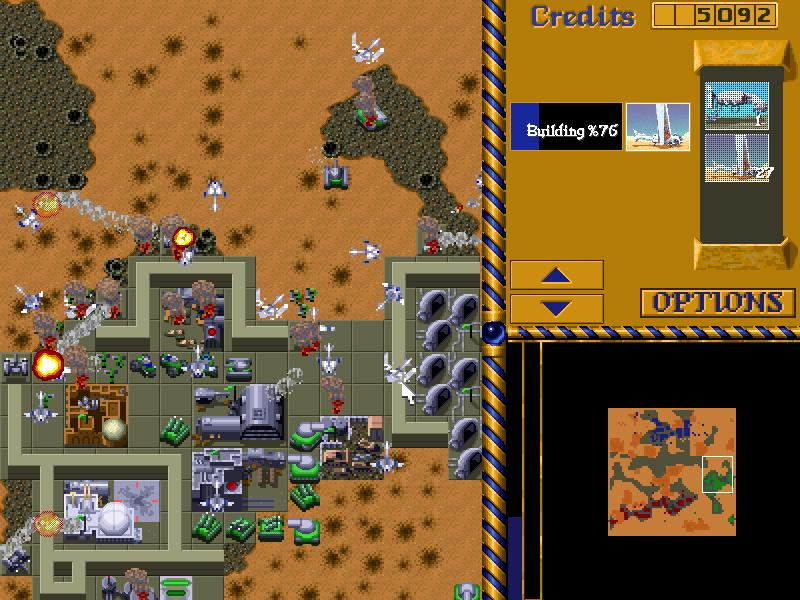
\includegraphics[scale=0.35]{Imagens/DuneII.jpg}
	\caption{Captura de tela de Dune II.}
	\label{fig:duneII}
\end{figure}

O jogador come�a o jogo com uma pequena quantidade de recursos, uma base e alguns soldados. Para poder enfrentar seu inimigo, ele dever� adquirir mais recursos atrav�s de unidades coletoras. Com estes recursos, ele ser� capaz de produzir unidades e estruturas que auxiliem em seus confrontos. Ap�s construir as estruturas obrigat�rias que permitem a coleta de recursos, o jogador se depara com a quantidade de op��es que ele pode executar:

\begin{itemize}
	\item Buscar no terreno outras fontes de recurso e/ou a localiza��o do oponente,
	\item Armazenar os recursos para constru��o de estruturas ou unidades mais caras,
	\item Produzir mais coletores,
	\item Criar unidades militares.
\end{itemize}

Al�m disso, existe a possibilidade de controlar as unidades enquanto elas est�o combatendo, para aumentar a efici�ncia delas no combate. Por se tratar de um jogo em tempo real, essas decis�es acabam por se tornar ainda mais complexas, pois o jogador deve constantemente: (a) refletir sobre quais aspectos ele deve focar, e (b) ser capaz de reagir ao que acontece na partida.

Ao construir mais estruturas e desbloquear novas unidades, o jogo avan�a de forma progressiva, expondo o jogador a desafios cada vez maiores conforme o tempo passa. Isto se deve � exist�ncia de um n�mero maior de estruturas de constru��o de unidades, mais unidades para controlar, mais unidades inimigas para combater e uma �rea maior para defender. Esse sentimento de progress�o dentro de uma partida passou a ser compartilhado por todos os RTS.

\subsection{Fases do Jogo}
As etapas conceituais de uma partida de qualquer RTS s�o nomeadas a partir das etapas das partidas de xadrez:
\begin{enumerate}
	\item Abertura
	\item Meio-jogo
	\item Final
\end{enumerate}

Assim como no xadrez, a abertura � uma s�rie de movimentos (no caso dos RTS, uma ordem de constru��o ou \emph{build order}) com a qual chega-se a uma posi��o desejada dentro do jogo. H� v�rios tipos de aberturas, comumente classificados como:
\begin{itemize}
	\item \emph{Cheese}: Abertura n�o-convencional desenvolvida para pegar o oponente de surpresa. Geralmente, \emph{cheese} � dif�cil de vencer se n�o for observado com anteced�ncia, mas f�cil de defender caso contr�rio.
	\item \emph{Rush}: Abertura que corta alguns custos a fim de produzir algum tipo de agress�o no in�cio do jogo. Normalmente a economia do jogador fica atrasada com rela��o ao esperado de outra abertura considerada mais tradicional.
	\item \emph{Greedy}: Aberturas gananciosas s�o similares aos \emph{rushes}, mas com um foco econ�mico. Essas aberturas podem ser punidas com um ataque na fase inicial do jogo, pois o jogador ter� cortado custos para desenvolver a economia, normalmente com a constru��o precoce de uma base. Caso n�o seja punida, essa abertura dar� ao jogador uma economia maior, o que possibilitar� um meio-jogo mais forte.
	\item \emph{Standard}: Este tipo de abertura foca inicialmente no desenvolvimento econ�mico, sem abrir m�o da defesa. Essas aberturas tendem a ser mais passivas, para defender-se de poss�veis \emph{cheeses} e \emph{rushes}.
\end{itemize}

A partir da abertura escolhida, e se o jogador n�o venceu ou perdeu o jogo devido a um \emph{cheese} ou \emph{rush}, pode ser poss�vel fazer uma transi��o para o meio-jogo. Para isso, avan�a-se na �rvore tecnol�gica de forma que o jogador consiga produzir uma composi��o s�lida de unidades, e ent�o parte-se para o ataque. Embora normalmente haja um foco �nico, isso n�o implica a utiliza��o de mais de um tipo de ataque durante o decorrer do jogo. Os principais tipos de ataques s�o:
\begin{itemize}
	\item Ataques � economia, atrav�s do transporte de unidades �s linhas de min�rio ou atrav�s de unidades de ass�dio\footnote{Unidades r�pidas e que podem causar grande dano econ�mico ao destruir muitos trabalhadores em pouco tempo.};
	\item Ataques em m�ltiplas localidades, para tentar reduzir o potencial de defesa do inimigo ao mesmo tempo em que foca-se na destrui��o de bases ou de estruturas de produ��o;
	\item Ataques frontais, for�ando o oponente a se preocupar mais em defender-se do que em aumentar seu lucro ou sua capacidade de produ��o.
\end{itemize}

O final do jogo � marcado pela escassez de recursos no mapa e pelo alto n�vel tecnol�gico dos jogadores, de forma que, geralmente, as batalhas envolvem uma disputa por recursos. Muito raramente as partidas chegam a esse est�gio, terminando em uma fase tardia do meio-jogo, quando pelo menos um dos jogadores chega ao �ltimo n�vel tecnol�gico.

A qualquer momento do jogo, como em um jogo de apostas, o jogador pode se colocar numa posi��o de ``tudo ou nada'', por ter ficado em uma posi��o de extrema desvantagem com rela��o ao outro jogador, seja na coleta de recursos, no desenvolvimento tecnol�gico ou na capacidade de produ��o. Assim, deve-se fazer algum ataque � economia ou produ��o do seu inimigo para conseguir ao menos deix�-lo em uma situa��o similar � sua, caso contr�rio n�o conseguir� vencer a partida.

\section{RTS em Intelig�ncia Artificial}
A partir do trabalho de \citeonline{buro03}, cujo foco � estimular pesquisas de intelig�ncia artificial em cima de RTS, muitos trabalhos foram feitos usando StarCraft como objeto de estudo. Como mostrado por \citeonline{ontanon13}, jogos deste g�nero s�o ambientes complexos, onde as t�cnicas de IA ainda t�m dificuldades, pois possui um espa�o de estados muito grande.

A complexidade de um ambiente pode ser classificada de acordo com v�rias propriedades \cite{russelnorvig}, e RTS se enquadra no pior caso na maior parte delas:
\begin{itemize}
	\item \textbf{Parcialmente observ�vel}: a n�voa de guerra impede o jogador de ver o que o oponente est� fazendo, e saber dados como sua taxa de coleta de recursos e a composi��o de seu ex�rcito, por exemplo, de antem�o.
	\item \textbf{Multiagente}: cada unidade do jogador possui um prop�sito e deve cooperar a fim de atingir objetivos globais. Da mesma forma, elas devem levar em conta as unidades inimigas que est�o no mapa e tentar combat�-las de alguma forma.
	\item \textbf{Estoc�stico}: embora o resultado de qualquer a��o de um agente seja determin�stico, o ambiente � parcialmente observ�vel, a quantidade de a��es que o oponente pode tomar � enorme e essas a��es podem ser feitas simultaneamente. Ele � complexo o bastante para ser considerado estoc�stico, ao inv�s de determin�stico.
	\item \textbf{Sequencial}: todas as a��es tomadas em um determinado momento da partida tem consequ�ncias, grandes ou pequenas, que se repercutem ao longo do jogo.
	\item \textbf{Din�mico}: o ambiente do jogo est� mudando constantemente com as a��es do jogador. Enquanto o jogador pensa no que fazer, jazidas de min�rios e g�iseres de g�s vespeno est�o se exaurindo, unidades s�o criadas e eliminadas, e unidades inimigas est�o se movimentando.
\end{itemize}

Jogos cl�ssicos, como Xadrez e Go, possuem uma grande complexidade com regras inteligentes e objetivos simples. Eles foram alvo de diversos trabalhos \cite{bouzy2001computer} devido � essa complexidade e simplicidade de regras. Conforme \citeauthor{ontanon13} explicam, jogos de estrat�gia em tempo real possuem uma complexidade muito superior �s complexidades destes dois jogos, que at� hoje s�o explorados por diversas t�cnicas de intelig�ncia artificial.

\begin{citacao}
Outra maneira de medir a complexidade do jogo � olhando o fator de ramifica��o, $b$, e a profundidade do jogo, $d$, [...] , com uma complexidade total de $b^d$. Em Xadrez, $b \approx 35$ e $d \approx 80$. Em jogos mais complexos, como Go, $b \approx 30$ a $300$, e $d \approx 150$ a $200$. A fim de determinar o fator de ramifica��o em StarCraft quando uma IA o joga, n�s devemos ter em mente que a IA pode dar a��es simultaneamente a quantas unidades no jogo for desejado. Ent�o, considerando que, em um jogo t�pico, um jogador controla entre $50$ e $200$ unidades, o fator de ramifica��o ficaria entre $u^{50}$ e $u^{200}$, onde $u$ � o n�mero m�dio de a��es que cada unidade pode executar. Estimar o valor de $u$ n�o � f�cil, pois o n�mero de a��es que uma unidade pode tomar � altamente dependente do contexto. [...] Agora, se tivermos em mente que a��es possuem tempos de \emph{cool-down}\footnote{Tempo de \emph{cool-down} � o tempo em que uma habilidade ou ataque fica indispon�vel entre um uso e outro. Esse conceito n�o se restringe aos RTS e pode ser observado em jogos como \emph{World of WarCraft}.}, e assim nem todas as unidades podem executar todas as a��es a todo quadro, podemos tomar uma estimativa conservadora de cerca de $10$ poss�veis a��es por unidade por quadro do jogo. Isto resulta em uma estimativa conservadora para o fator de ramifica��o entre $b \in [10^{50}, 10^{200}]$, somente considerando unidades (ignorando as a��es que constru��es podem executar). Agora, para computar $d$, n�s simplesmente consideramos o fato de que os jogos t�picos duram em torno de 25 minutos, o que resulta em $d \approx 36000$ (25 minutos $\times$ 60 segundos $\times$ 24 quadros por segundo) \cite[p. 294]{ontanon13}.
\end{citacao}

Esta compara��o de complexidade (mais evidente na Tabela~\ref{tab:complex}), mostra uma diferen�a grande entre a quantidade de estados dos jogos. Devido a esse fator, pesquisadores como \citeauthor{buro03} e \citeauthor{ontanon13} acreditam que o investimento de pesquisas com foco em jogos de estrat�gia em tempo real possibilitam um amplo melhoramento ou cria��o de t�cnicas de intelig�ncia artificial.

\begin{table}[h]
	% T�tulo de tabelas sempre aparecem antes da tabela
	\center
	{
		\begin{tabular}{l|l|l}
			\hline
			\textbf{Jogo} & \textbf{Fator de ramifica��o} & \textbf{Profundidade do jogo}\\
			\hline
			Xadrez & $\approx 35$ & $\approx 80$\\
			Go & $\approx 30$ a $300$ & $\approx 150$ a $200$\\
			StarCraft (25 minutos) & $[10^{50}, 10^{200}]$ & $\approx 36000$\\
			\hline
		\end{tabular}
	}
	\caption{Compara��o das complexidades de jogos abordados atrav�s de IA e um RTS.}
	\label{tab:complex}
\end{table}

\subsection{Desafios em RTS}
No intuito de estimular pesquisas de intelig�ncia artificial em RTS, \citeonline{buro03} observou seis desafios encarados ao tentar criar uma \emph{game AI} para um jogo desse g�nero:
\begin{enumerate}
	\item \textbf{Gerenciamento de recursos}: desafio que envolve a coleta e o gasto dos recursos, seja em unidades, tecnologias ou estruturas, em um ambiente mut�vel e em tempo real.
	\item \textbf{Tomada de decis�o sob incerteza}: devido � n�voa de guerra (\emph{fog of war}), n�o � poss�vel saber a localiza��o e inten��es do(s) oponente(s), e o jogador deve tomar decis�es sem esse conhecimento.
	\item \textbf{Racioc�nio temporal e espacial}: an�lises de terreno est�tica e din�mica bem como entender a rela��o temporal das a��es � imprescind�vel no decorrer do jogo.
	\item \textbf{Colabora��o}: em partidas cooperativas, duas \emph{game AIs} aliadas devem saber interagir de modo a vencer a partida.
	\item \textbf{Modelagem e aprendizado de oponentes}: ao enfrentar o mesmo oponente v�rias vezes, \emph{game AIs} devem conseguir se adaptar ao seu estilo de jogo.
	\item \textbf{Planejamento advers�rio em tempo real}: ao inv�s de planejar micro-a��es, a \emph{game AI} deve utilizar abstra��es para manter o espa�o de busca em tamanho gerenci�vel.
\end{enumerate}

Ap�s 10 anos de publica��o do trabalho de \citeauthoronline{buro03} e v�rios artigos sobre StarCraft e seu g�nero, \citeonline{ontanon13} expuseram os seis atuais desafios na cria��o de \emph{game AI} para RTS:
\begin{enumerate}
	\item \textbf{Planejamento}: o planejamento em RTS depende de m�ltiplos n�veis de abstra��o.	No n�vel mais elevado, o jogador precisa ter capacidades de planejamento a longo prazo, para desenvolver uma economia forte no jogo; no n�vel mais baixo, as unidades devem ser controladas levando em considera��o o terreno e o oponente.
	\item \textbf{Aprendizado}: os autores distinguiram tr�s tipos de problemas de aprendizado em jogos de estrat�gia em tempo real:
	\begin{itemize}
		\item \emph{Aprendizado a priori}: o aprendizado que se faz antes da partida come�ar, analizando \emph{replays} ou mapas para aprender as estrat�gias apropriadas.
		\item \emph{Aprendizado na partida}: implanta��o de t�cnicas de aprendizado \emph{online}, como aprendizado por refor�o e modelagem de oponentes, para adaptar-se em tempo real.
		\item \emph{Aprendizado entre partidas}: estudar o que aconteceu nas �ltimas partidas e usar esse conhecimento para aumentar as chances de vit�ria nas pr�ximas partidas.
	\end{itemize}
	\item \textbf{Incerteza}: em RTS existem dois principais tipos de incerteza. O primeiro � pelo jogo ser parcialmente observ�vel, for�ando o jogador a patrulhar para saber o que o oponente est� fazendo. O segundo � pelo jogo ser competitivo e o jogador n�o conseguir predizer as a��es do(s) oponente(s).
	\item \textbf{Racioc�nio temporal e espacial}: racioc�nio espacial engloba cada aspecto da explora��o do terreno. Est� relacionado a posicionamento de estruturas, expans�o de bases e controle de unidades. O posicionamento de estruturas pode ajudar o jogador a criar as constru��es de forma a proteger sua base ou evitar configura��es que impe�am unidades de mover. Antes de criar novas bases, o jogador precisa avaliar as possibilidades e escolher o melhor posicionamento, levando em considera��o as suas bases e as do oponente. O controle das unidades no campo de batalha deve evitar ficar em gargalos e posicionando as unidades de maneira favor�vel, como um terreno elevado.
	\item \textbf{Explora��o do conhecimento de dom�nio}: como a quantidade de conhecimento de dom�nio � significativamente grande, n�o se sabe como esse conhecimento pode ser explorado por \emph{game AIs}. Os trabalhos se focaram em: (a) implementar as estrat�gias existentes diretamente nas \emph{game AIs}, e (b) analisar grandes conjuntos de \emph{replays} para aprender estrat�gias, tend�ncias ou planos.
	\item \textbf{Decomposi��o de tarefas}: por todas as raz�es acima, a maior parte dos trabalhos decomp�e o problema em uma cole��o de pequenos problemas, a serem resolvidos independentemente.  A divis�o mais comum �:
	\begin{itemize}
		\item \emph{Estrat�gia}: est� relacionada com a �rea mais elevada do processo de tomada de decis�o. Deve identificar estrat�gias eficientes contra um dado oponente.
		\item \emph{T�tica}: implementa a estrat�gia escolhida de forma eficiente. Cuida de movimenta��o do ex�rcito, posicionamento de constru��es, timings de ataques e produ��es.
		\item \emph{Controle reativo}: implementa��o das t�ticas. Determina os alvos das unidades, sua movimenta��o em batalha e fuga.
		\item \emph{An�lise de terreno}: consiste em identificar pontos importantes no mapa e saber as regi�es naveg�veis dentro dele. Pontos importantes incluem posi��es de min�rios e g�s, gargalos, terrenos elevados ou rebaixados.
		\item \emph{Coleta de informa��o}: devido � n�voa de guerra, jogadores devem regularmente mandar patrulhas para localizar e espionar bases inimigas.
	\end{itemize}
	Por�m como integrar todas essas �reas em uma �nica arquitetura ainda � um problema aberto.
\end{enumerate}

\subsection{Trabalhos Existentes}
Durante os �ltimos anos, v�rios trabalhos cient�ficos focaram nas diferentes �reas desse jogo.
\begin{itemize}
	\item Na �rea que cuida da produ��o de unidades e da pesquisa de tecnologias, trabalhos focaram em abordagens baseadas em aprendizado de m�quina \cite{weber09} \cite{deres11} \cite{synn11} \cite{young12} \cite{hsieh08}.
	\item Na �rea de an�lise de terreno \citeonline{perkins10} encontrou uma maneira de identificar as regi�es naveg�veis e separou-as atrav�s de gargalos, tamb�m identificados pela decomposi��o de Voronoi.
	\item Em posicionamento de estruturas, \citeonline{certicky13} apresentou uma abordagem para isso usando \emph{answer-set programming}.
	\item Outra �rea que foi foco de v�rios trabalhos � a �rea de controle de unidades militares. Dessa �rea, pode-se dividir os trabalhos focados na �rea de decis�o e na �rea de movimenta��o. Trabalhos na �rea de decis�o usaram \emph{case-based reasoning} \cite{cadena11} \cite{synn12} para o planejamento t�tico.
	\item Trabalhos sobre movimenta��o utilizaram \emph{potential fields} \cite{sajjad11} \cite{hagelback12} e aprendizado por refor�o \cite{wender12}.
\end{itemize}

Mais refer�ncias de artigos que utilizam esse jogo como objeto de estudo podem ser vistos no trabalho de \citeonline{ontanon13}.

\subsection{Competi��es de Bots}
Com a cria��o de uma \abrv[API -- Application Programming Interface]{API} que permitiu fazer interface entre o jogo StarCraft e sistemas desenvolvidos para controlar automaticamente os personagens deste jogo, pesquisadores em \emph{game AI} criaram um \emph{framework} de competi��es entre diferentes sistemas que substituem o jogador humano. As competi��es come�aram em 2010 nas confer�ncias cient�ficas \abrv[AIIDE -- AAAI Conference on Artificial Intelligence and Interactive Digital Entertainment]{AIIDE} e \abrv[CIG -- IEEE Conference on Computational Intelligence and Games]{CIG}, organizadas respectivamente pela AAAI (\emph{Association for Advancement of Artificial Intelligence}) e pela IEEE (\emph{Institute of Electrical and Electronics Engineers}). Outras duas competi��es surgiram nos anos seguintes. A \abrv[SSCAI -- Student StarCraft AI Tournament]{SSCAI}\footnote{\url{http://sscaitournament.com}} surgiu em 2011 com a ideia de fazer uma competi��o entre \emph{game AIs} feitas por estudantes, e entre as feitas pelos estudantes contra o estado da arte. Em 2012, foi criada a liga de rob�s de StarCraft, \emph{StarCraft BroodWar Bots Ladder}\footnote{\url{http://bots-stats.krasi0.com/}} que visa ser um ambiente de competi��o ininterrupta e cont�m 17 \emph{bots} classificados de acordo com o sistema de \emph{ranking} Elo. Detalhes sobre as competi��es da AIIDE, CIG e sobre a liga podem ser vistos em  \cite{ontanon13}.

%\subsubsection{AIIDE}
%Desde 2010, a AIIDE organiza a competi��o \emph{AIIDE StarCraft AI Competition}, a mais conhecida e mais antiga competi��o de IA para StarCraft do mundo \cite{ontanon13}. A cada ano, os competidores colocam seus rob�s para batalhar em vers�es normais de StarCraft: Brood War, com pr�mios fornecidos pela Blizzard Entertainment.
%
%Inicialmente, a competi��o da AIIDE era dividida em quatro torneios distintos. O Torneio 1 era um torneio de microgerenciamento de unidades em um terreno plano. O Torneio 2, era tamb�m de microgerenciamento mas em um terreno irregular. O Torneio 3 envolvia o macrogerenciamento mas com tecnologias limitadas, em um mapa espec�fico. O Torneio 4 era um torneio com partidas completas em mapas aleat�rios. Essa �ltima modalidade continua at� hoje. Como em competi��es de jogadores humanos, nenhuma IA pode trapacear ou usar determinados \emph{bugs} para obter vantagem.
%
%No primeiro ano de competi��es, o vencedor da competi��o foi o rob� Overmind, da Universidade da Calif�rnia, que usou grandes n�meros de mutalisks controladas por um sistema de microgerenciamento baseado em \emph{potential fields}. O rob� krasi0 ficou em segundo lugar, jogando mais tradicionalmente e optando pela estrat�gia \emph{mech} dos Terran. Nesse torneio, foi utilizado o formato de elimina��o dupla, cada partida sendo uma melhor de 5.
%
%No segundo ano, com a introdu��o de um sistema de gerenciamento de torneios automatizado, o torneio optou por utilizar o estilo \emph{round-robin}. Este torneio teve um grande n�mero de \emph{bots} jogando com os Protoss, seis dos 13 rob�s que jogaram eram dessa ra�a. Tr�s desses ficaram nos tr�s primeiros lugares, Skynet, UAlbertaBot e AIUR, respectivamente. Ap�s essa competi��o, houve uma partida homem vs. m�quina, entre o vencedor da competi��o, Skynet, e um ex-jogador profissional. Esse jogador escolheu ra�as aleat�rias em cada partida, da melhor de tr�s. A performance do \emph{bot} mostrou que n�o havia preparo nem adapta��o para enfrentar um jogador humano de alto n�vel, e Skynet perdeu por 2-0.
%
%Em 2012, foi introduzida a possibilidade de salvar informa��es em disco, entre partidas. Neste ano, Skynet ganhou mais uma vez, com AIUR em segundo lugar e UAlbertaBot em terceiro. Na partida homem vs. m�quina, o jogador humano escolhido foi Bakuryu, na �poca um dos melhores Zerg n�o-coreanos do mundo. Isso foi mostrado nas partidas contra Skynet, onde ele fez a IA parecer muito boba, usando seus zerglings para tirar a aten��o dos zealots\footnote{Primeira unidade militar \emph{protoss}, capaz de atacar somente a corpo-a-corpo.} e de metade dos trabalhadores da Skynet ao deix�-los correndo em c�rculos ao redor da base do \emph{bot}. Depois de matar v�rios trabalhadores, ele limpou o ex�rcito inimigo com um grupo de mutalisks. Isso mostrou que os sistemas de IA para StarCraft ainda n�o conseguiram ter um racioc�nio de causa e consequ�ncia. Pois os zerglings estavam desviando a aten��o da IA para dar tempo das mutalisks serem criadas e atacarem.
%
%\subsubsection{CIG}
%Inicialmente, em 2010, a CIG organizou um torneio de IA para StarCraft por�m sofreu problemas t�cnicos. Devido a quantidade de \emph{crashes} com os mapas escolhidos, que n�o foram testados a priori, se tornou injustific�vel eleger um vencedor.
%
%Em 2011, 
%
%
%\subsubsection{SSCAI}
%
%
%\subsubsection{Liga de Rob�s}

\section{Objetivos}
Apesar do crescente n�mero de \emph{game AIs} que apareceram nas competi��es acad�micas e a possibilidade de v�-las funcionando em tempo real, pela SSCAI, ainda percebe-se um negligenciamento do estudo do funcionamento das mentalidades dos jogadores profissionais. Com o intuito de estudar este problema, esse trabalho prop�e um modelo que trata de diferentes �reas de interesse a fim de criar uma \emph{game AI} que consiga agir de acordo com os comportamentos vistos em campeonatos profissionais de StarCraft.

Ao analisar a demografia das \emph{game AIs} que entraram nas competi��es AIIDE 2011, AIIDE 2012 e CIG 2011, foi constatado que havia poucas solu��es voltadas ao tratamento da ra�a \emph{Zerg}. Al�m disso, as estrat�gias adotadas por essas \emph{game AIs} eram muito pouco variadas, e at� mesmo mal geridas de acordo com o confronto. Juntando com o fato do autor deste trabalho ter uma grande experi�ncia pr�tica jogando com essa ra�a, a decis�o de me aventurar com os \emph{Zerg} foi natural. Devido � complexidade dos confrontos, que requer \emph{mindsets}\footnote{Conjuntos de suposi��es e atitudes.} diferentes quando se joga contra cada ra�a, o projeto se focar� nas partidas contra a ra�a Terran. 

Este trabalho tem como objetivo principal comparar as aberturas mais usadas pelos jogadores profissionais no confronto Zerg versus Terran atrav�s do ponto de vista econ�mico e militar, observando a coleta de recursos e o tempo de cria��o das primeiras unidades militares.

O conjunto de aberturas poss�veis da \emph{game AI} foi escolhido a partir de uma entrevista com Mike Lange, um jogador Zerg de alto n�vel, que j� ajudou na avalia��o de \emph{game AI} de StarCraft em campeonatos da AIIDE \cite{ontanon13}. Ele exp�s as aberturas usadas por todas as estrat�gias que foram consolidadas em torneios profissionais. Dentre todas essas aberturas, apenas algumas foram selecionadas:
\begin{itemize}
	\item \emph{5 pool}: um \emph{cheese} que consiste em criar v�rias unidades militares no in�cio do jogo;
	\item \emph{9 pool}: um \emph{rush} menos agressivo que a \emph{5 pool}, mas mais seguro e com o potencial de negar expans�es territoriais do inimigo por um bom per�odo de tempo;
	\item \emph{Overpool}: uma abertura mais econ�mica que pode fazer o inimigo achar que se trata de uma \emph{9 pool};
	\item \emph{12 pool}: uma abertura mais defensiva, boa para prevenir contra \emph{rushes} da ra�a Terran;
	\item \emph{12 hatch}: a abertura mais tradicional, que possibilita transi��es s�lidas para o meio-jogo.
\end{itemize}

Pela entrevista com o jogador, algumas hip�teses foram criadas:
\begin{enumerate}
	\item As aberturas possuem taxas de coleta diferentes. Elas podem ser ordenadas em forma crescente, de acordo com esta taxa, da seguinda maneira: \emph{5 pool}, \emph{9 pool}, \emph{overpool}, \emph{12 pool} e \emph{12 hatch}.
	\item As aberturas tamb�m possuem tempos de cria��o de \emph{zerglings} diferentes. A ordem crescente das aberturas pelo tempo de cria��o destas unidades � descrita por: \emph{5 pool}, \emph{9 pool}, \emph{overpool}, \emph{12 pool} e \emph{12 hatch}.
\end{enumerate} 

Para atingir este objetivo, a \emph{game AI} deve ser capaz de realizar as atividades: (a) manter uma ordem de constru��o e execut�-la, (b) coletar min�rios com os trabalhadores, (c) posicionar e construir estruturas e (d) identificar locais de expans�o. Com base nisto, os objetivos secund�rios desse trabalho s�o:
\begin{itemize}
	\item Criar um sistema que maximize a quantidade de recursos explorados em um determinado per�odo de tempo,
	\item Criar um sistema de posicionamento e constru��o de estruturas que dificulte ao acesso dos inimigos � base,
	\item Criar um sistema que defina uma sequ�ncia de expans�o territorial adequada � estrat�gia adotada no jogo.
\end{itemize}

\section{Organiza��o do trabalho}
O restante deste trabalho est� dividido em:
\begin{itemize}
	\item Cap�tulo 2: apresenta��o dos problemas espec�ficos do jogo StarCraft.
	\item Cap�tulo 3: o modelo conceitual do sistema que ir� controlar os personagens do jogo.
	\item Cap�tulo 4: a aplica��o do modelo no jogo StarCraft, voltada � ra�a Zerg.
	\item Cap�tulo 5: os resultados dos experimentos feitos com a implementa��o.
	\item Cap�tulo 6: apresenta��o de conclus�es e trabalhos futuros.
\end{itemize}


\chapter{StarCraft}
% \subsection{\emph{Timeline} dos RTS}
% 
% Ap�s Dune II, v�rios outros t�tulos menos expressivos foram lan�ados, at� que em 1994 a Blizzard Entertainment lan�ou WarCraft: Orcs \& Humans (Figura~\ref{fig:warcraft}), onde o jogador deve escolher entre as ra�as \emph{orc} ou humana para jogar. Este jogo teve um foco mais voltado ao gerenciamento das unidades, apresentando conjuradores (\emph{spellcasters}), unidades que n�o possuem uma forma de ataque direto, tendo que gastar uma quantidade de energia de um reservat�rio pessoal para usar alguma habilidade especial. Al�m disso, ele apresenta dois recursos, ao inv�s de um.
% 
% \begin{figure}[H]
% 	\centering
% 	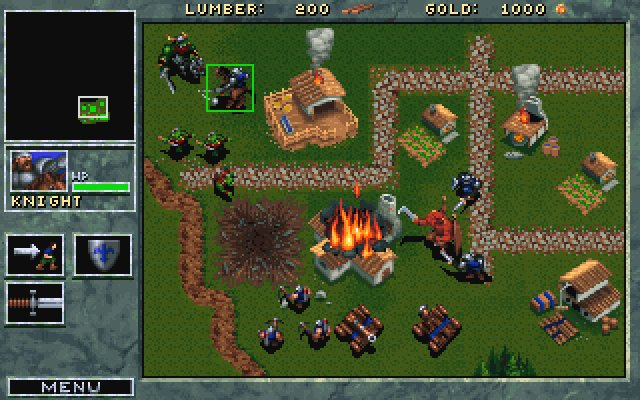
\includegraphics[scale=0.4]{Imagens/warcraft.jpg}
% 	\caption{Captura de tela de WarCraft.}
% 	\label{fig:warcraft}
% \end{figure}
% 
% Em 1995, a Virgin Interactive lan�ou Command \& Conquer (Figura~\ref{fig:cnc}), desenvolvido pela Westwood Studios. Nele existem duas fac��es que n�o s�o sim�tricas, ao contr�rio de todos os jogos de estrat�gia em tempo real da �poca, e que s�o equilibradas de forma que suas for�as se sobrep�em sobre suas fraquezas. Nele o jogador escolhe entre as fac��es: \emph{Global Defense Initiative} (GDI) e \emph{Brotherhood of Nod} (Nod). As unidades da GDI s�o mais resistentes e poderosas, por�m mais caras que as da Nod. Al�m disso, o estilo de jogo da GDI � focado em ataques estrat�gicos de larga escala, enquanto a Nod procura usar t�ticas n�o convencionais \cite{cirulis95}.
% 
% \begin{figure}[H]
% 	\centering
% 	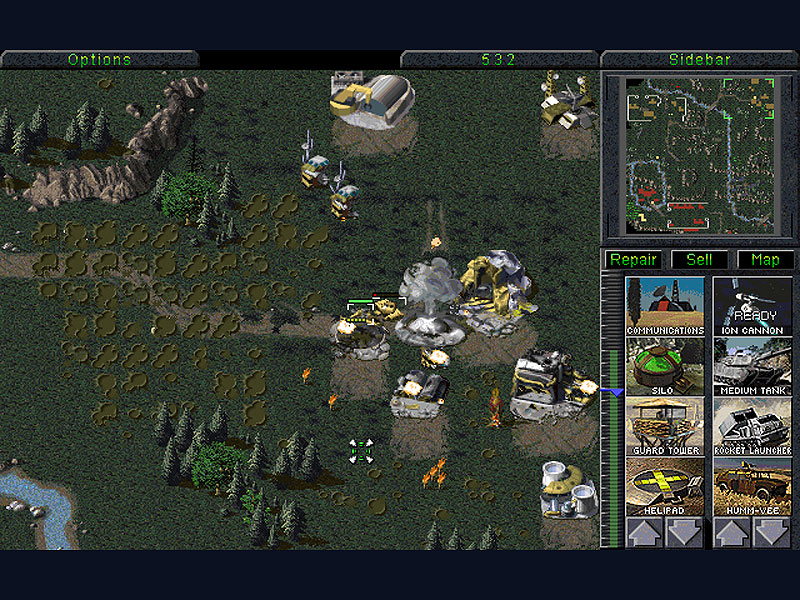
\includegraphics[scale=0.32]{Imagens/cnc.jpg}
% 	\caption{Captura de tela de Command \& Conquer.}
% 	\label{fig:cnc}
% \end{figure}
% 
% No ano seguinte, a BlueByte lan�ou The Settlers II (Figura~\ref{fig:settlersII}), jogo criado pela pr�pria empresa. Esse jogo foge quase que inteiramente do padr�o de jogos de estrat�gia em tempo real, pois n�o d� ao jogador o controle das unidades nem o controle direto da produ��o delas. Ao inv�s disso, o jogador tem controle sobre onde as constru��es ser�o constru�das e quais caminhos os trabalhadores ir�o tomar, pois as constru��es s�o ligadas por estradas at� o castelo principal. Al�m disso, existem 31 recursos, entre recursos brutos e recursos produzidos, que permitem a cria��o de unidades e constru��es. O que o jogador pode fazer para influenciar a cria��o de unidades � alterar a taxa com que os produtos necess�rios para a cria��o de cada unidade sejam produzidos. As batalhas s�o feitas automaticamente, por�m o jogador escolhe quando e onde atacar.
% 
% \begin{figure}[H]
% 	\centering
% 	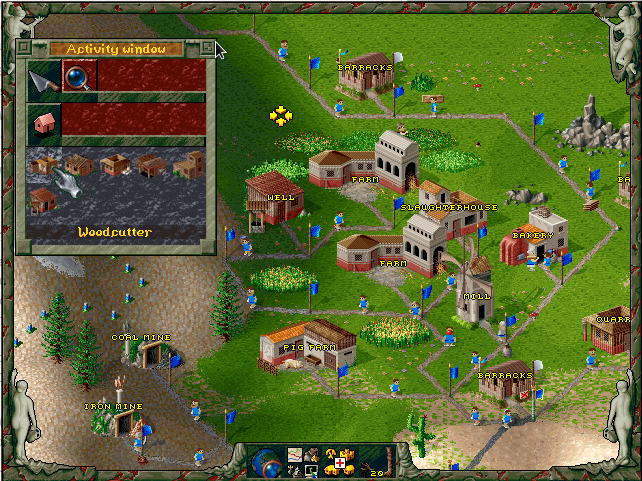
\includegraphics[scale=0.4]{Imagens/Settlers2.png}
% 	\caption{Captura de tela de The Settlers II.}
% 	\label{fig:settlersII}
% \end{figure}
% 
% Posteriormente, Total Annihilation\footnote{\url{http://web.archive.org/web/20010405091547/http://cavedog.com/totala/index.html}} (Figura~\ref{fig:totala}) foi lan�ado pela GT Interactive em 1997, desenvolvido pela Cavedog Entertainment. Total Annihilation trouxe duas fac��es que pilotam ve�culos de batalha gigantescos e disputam planetas para conquistar os recursos \emph{metal} e \emph{energia}. Foi o primeiro jogo a apresentar unidades e terreno 3D. Bem como os outros jogos, as partidas s�o jogadas em mapas retangulares e existem posi��es de extra��o de recursos. Ao contr�rio de todos os outros jogos, o consumo de recursos n�o se d� de uma s� vez. O jogador ``paga'' cada unidade e cada estrutura ao longo do tempo, e do mesmo modo a coleta n�o � feita atrav�s de pequenos peda�os, mas ela � cont�nua em uma taxa constante. Unidades e estruturas possuem diferentes taxas de coleta ou de consumo de recursos, sendo necess�rio fazer um balan�o entre a entrada e a sa�da deles. Al�m disso, o jogo fornece ao jogador uma unidade que serve como ``base'' inicial, chamada Comandante. Esse comandante � a chave da vit�ria pois o objetivo das partidas � destruir o comandante inimigo.
% 
% \begin{figure}[H]
% 	\centering
% 	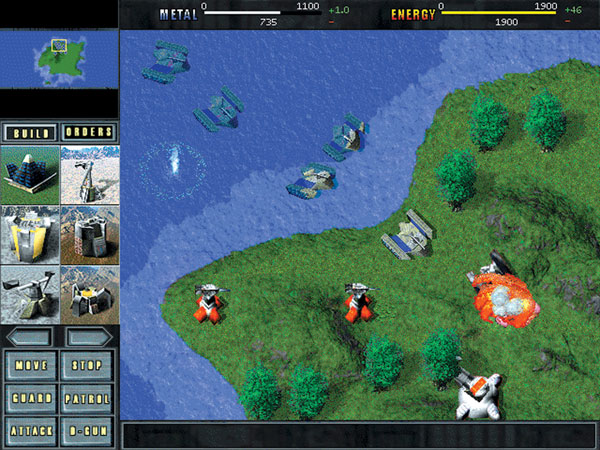
\includegraphics[scale=0.4]{Imagens/totala.jpg}
% 	\caption{Captura de tela de Total Annihilation.}
% 	\label{fig:totala}
% \end{figure}
% 
% Lan�ado no mesmo ano, Age of Empires\footnote{\url{http://www.ageofempires.com/}} (Figura~\ref{fig:aoe}), distribu�do pela Microsoft Game Studios e desenvolvido pela Ensemble Studios, leva o jogador � Idade da Pedra para jogar com uma das civiliza��es dispon�veis. Tr�s civiliza��es de cada regi�o do mundo antigo estavam presentes. Elas podem ser classificadas como mediterr�neas, mesopot�mias orientais e ocidentais, e asi�ticas. Ao inv�s de um ou dois recursos, o jogo apresenta quatro recursos ao jogador: comida, madeira, ouro e pedra. Esse jogo trouxe a possibilidade de cria��o de fazendas, estruturas que custam madeira e permitem a coleta de comida, sendo o primeiro jogo a fazer uma efetiva troca de recursos. Al�m disso, a evolu��o tecnol�gica do jogador � marcada por tecnologias de passagem de era, pesquisadas na \emph{town center}, estrutura que serve de dep�sito para a coleta de recursos. Nesta estrutura tamb�m s�o criados os \emph{trabalhadores}\footnote{Unidade b�sica que pode construir e coletar recursos.} e pesquisas relacionadas � essas unidades. Esse tipo de estrutura � chamado de estrutura-base ou simplesmente base. Conforme o jogador avan�a sua era, novas constru��es e tecnologias s�o desbloqueadas. As eras do jogo s�o: Idade da Pedra, Idade da Ferramenta, Idade do Bronze e Idade do Ferro.
% 
% \begin{figure}[H]
% 	\centering
% 	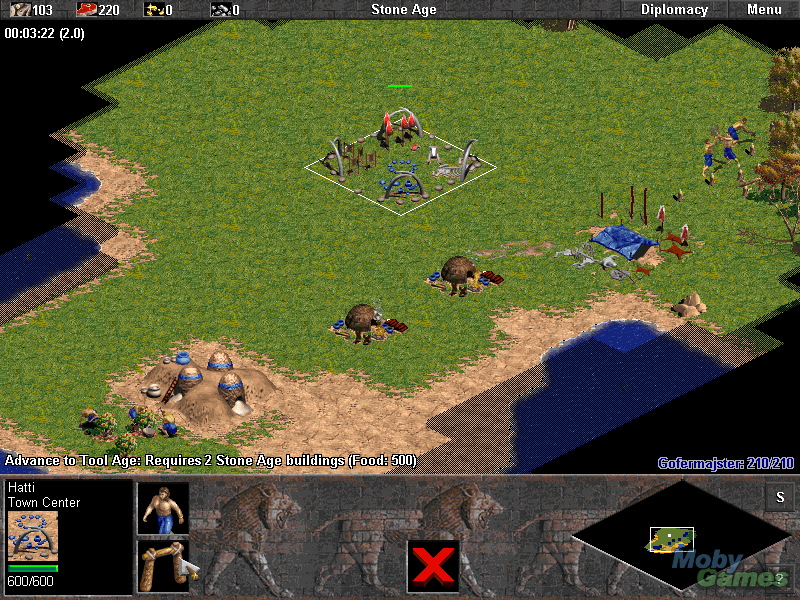
\includegraphics[scale=0.32]{Imagens/aoe.png}
% 	\caption{Captura de tela de Age of Empires.}
% 	\label{fig:aoe}
% \end{figure}
% 
% Em 1998, a Blizzard Entertainment lan�ou StarCraft (Figura~\ref{fig:sc}) e em seguida sua expans�o, Brood War, que traz novas unidades e tecnologias que procuram dar um suporte maior �s unidades existentes\footnote{\url{http://classic.battle.net/scc/popup/airbal.htm}}.
% 
% \begin{figure}[H]
% 	\centering
% 	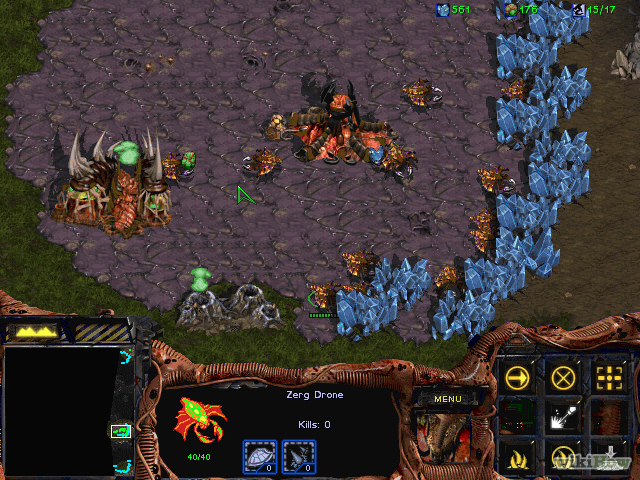
\includegraphics[scale=0.4]{Imagens/Base.jpg}
% 	\caption{Captura de tela de StarCraft.}
% 	\label{fig:sc}
% \end{figure}
% 
% \section{StarCraft}
StarCraft � um RTS em que o jogador deve coletar dois tipos de recursos, \emph{min�rios} e \emph{g�s vespeno}, para poder enfrentar um grupo de inimigos. Esses recursos s�o normalmente distribu�dos pelo mapa de forma tal que se possa criar uma base de extra��o, tamb�m chamada de expans�o, pr�xima a todas as fontes de recursos\footnote{Estruturas neutras que s�o o alvo da coleta de recursos.}, jazidas de min�rios e g�iseres de g�s vespeno (Figura~\ref{fig:resources}). O conjunto de jazidas de min�rios pr�ximo a uma base � chamado de linha de min�rio.

\begin{figure}[H]
	\centering
	\subfloat[Jazidas de min�rios]{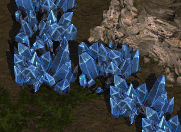
\includegraphics[scale=0.66]{Imagens/minerals.jpg}}
	\qquad
	\subfloat[G�iser de g�s vespeno]{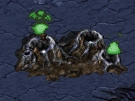
\includegraphics[scale=0.012]{Imagens/Vespene.jpg}}
	\caption{Recursos de StarCraft.}
	\label{fig:resources}
\end{figure}

Desses recursos naturais, os min�rios s�o os principais, usados para produ��o de todas as unidades, estruturas e pesquisas dentro do jogo. O g�s vespeno, por sua vez, � usado para unidades especiais e pesquisas tecnol�gicas. Para aquisi��o desses recursos s�o necess�rios trabalhadores, que se encarregar�o de coletar os recursos a partir de alguma fonte e entreg�-los � base mais pr�xima.

Al�m de recursos naturais, o jogador precisa de recursos secund�rios. Dentre estes recursos secund�rios, os mais not�rios s�o os \emph{suprimentos}, sem os quais n�o � poss�vel produzir unidades. Cada unidade consome uma quantidade pr�-determinada de suprimentos, e para poder produzir mais unidades � necess�ria a cria��o de mais fontes de suprimento, at� que se chegue na capacidade m�xima determinada pelo jogo. Outro recurso secund�rio � o \emph{tempo}, uma vez que toda produ��o e movimenta��o est� restrita ao tempo que vai ser levado para termin�-los.

A cria��o de unidades, incluindo trabalhadores, � feita em estruturas de produ��o. Essas estruturas podem ter pr�-requisitos estruturais, como por exemplo a \emph{factory}\footnote{Estrutura de produ��o da ra�a Terran que produz unidades de ataque terrestres mec�nicas.} que necessita de uma \emph{barracks}\footnote{Estrutura de produ��o da ra�a Terran que produz soldados.} para ser constru�da. Unidades tamb�m podem ter esses pr�-requisitos, como o \emph{dragoon}\footnote{Unidade de ataque terrestre da ra�a Protoss que tem a capacidade de atingir unidades a�reas e terrestres.} que precisa da \emph{cybernetics core}\footnote{Estrutura de pesquisa da ra�a Protoss que se encarrega das tecnologias de ataque e defesa das unidades a�reas.}. As estruturas de produ��o, bem como as estruturas de pesquisa, possuem uma fila de produ��o com a qual pode-se antecipar a ordem de constru��o de alguma unidade ou pesquisa, isto �, sem precisar futuramente mandar a estrutura produzir no tempo exato. Isso ajuda o jogador a otimizar o tempo em algumas situa��es, como quando ele quer produzir muitas unidades.

Antes de cada partida, o jogador deve escolher uma entre tr�s ra�as, cada uma com suas pr�prias �rvores tecnol�gicas e peculiaridades. As ra�as dispon�veis s�o:
\begin{itemize}
	\item \emph{Protoss}: � uma ra�a que possui unidades muito resistentes e com elevado poder de fogo, por�m consomem muito de todos os recursos - min�rios, g�s, suprimento e tempo - para serem produzidas. Suas estruturas de produ��o s�o especializadas: \emph{gateway} � encarregado de produzir as unidades terrestres b�sicas de ataque, a \emph{robotics facility} produz unidades utilit�rias, isto �, unidades que precisam de unidades b�sicas para que seu uso no ex�rcito tenha sentido, e o \emph{stargate} produz unidades a�reas de ataque. Sua estrutura-base � o \emph{nexus}.
	\item \emph{Zerg}: voltada a produzir muitas unidades de uma s� vez, esta ra�a possui as unidades mais fr�geis e mais baratas do jogo. Ao contr�rio das outras ra�as, ela possui apenas uma estrutura de produ��o, que tamb�m � sua estrutura-base, a \emph{hatchery}. A \emph{hatchery} gera larvas, unidades especiais que servem apenas para produzir outras unidades, e n�o possui fila de produ��o, de forma que � poss�vel produzir v�rias unidades ao mesmo tempo.
	\item \emph{Terran}: � uma ra�a parecida com os Protoss, por�m mais vers�til. Um meio termo entre Protoss e Zerg, j� que possui unidades baratas e fr�geis, mas com sua produ��o limitada a estruturas de produ��o semelhantes �s dos Protoss. Os Terran possuem dois tipos de estrat�gias consolidados, um baseado nas unidades feitas nas \emph{barracks} e outro baseado nas unidades feitas na \emph{factory}. As estrat�gias baseadas em \emph{barracks} se chamam \emph{Bio Terran} ou somente \emph{Bio}, e as baseadas em \emph{factory} se chamam \emph{Mech Terran} ou somente \emph{Mech}.
\end{itemize}

\section{Competi��o em StarCraft}
StarCraft: Brood War � um dos jogos mais bem sucedidos da hist�ria tanto em popularidade, tendo vendido mais de 11 milh�es de c�pias at� 2009 \cite{graft09}, como em tempo de competi��o profissional. Por mais de dez anos, este jogo foi jogado profissionalmente na Coreia do Sul em v�rias ligas, como a \abrv[OSL -- OnGameNet Starleague]{OSL} (OnGameNet Starleague)\footnote{\url{http://wiki.teamliquid.net/starcraft/OnGameNet_Starleague_(OSL)}}, bem como no evento internacional de esportes eletr�nicos World Cyber Games, desde do ano 2000 na WCG Challenge\footnote{\url{https://web.archive.org/web/20020709193219/http://www.worldcybergames.org/challenge/summary.asp}} at� a WCG 2010\footnote{\url{http://wiki.teamliquid.net/starcraft/WCG_2010}}.

Durante esse per�odo, as competi��es acompanharam a evolu��o das estrat�gias de cada uma das ra�as. Um exemplo dessa evolu��o � o conjunto das estrat�gias usadas pelos jogadores Zerg contra jogadores Terran nas competi��es. Durante um certo per�odo as estrat�gias mais usadas pelos Terran dominaram as estrat�gias usadas pelos Zerg. Com a cria��o e populariza��o de uma abertura chamada \emph{3 Hatch Muta} pelo jogador sAviOr\footnote{\url{http://wiki.teamliquid.net/starcraft/Metagame}}, que � a cria��o de 3 \emph{hatcheries} e sua transi��o para a cria��o de \emph{mutalisks}\footnote{Unidade a�rea de ass�dio \emph{zerg} capaz de atingir alvos a�reos e terrestres.} para atingir a economia do oponente, foi constatado um aumento na taxa de vit�rias Zerg nas competi��es, levando essa ra�a a ter uma vantagem contra os Terran.

O estado atual das estrat�gias mais usadas � chamado de \emph{metagame}, ou metajogo, e � influenciado tanto pelos mapas que est�o sendo jogados nas competi��es bem como pelas estrat�gias usadas pelos potenciais advers�rios, como visto anteriormente. Um exemplo de mudan�a de metajogo devido aos mapas aconteceu com o mapa Destination\footnote{\url{http://wiki.teamliquid.net/starcraft/Destination}}, no confronto Protoss versus Zerg (PvZ). Por um tempo, os Protoss estiveram com uma porcentagem favor�vel de vit�rias no mapa, por�m os jogadores Zerg descobriram uma ordem de constru��o que melhor se adaptava ao mapa e conseguiram reverter a situa��o, vencendo 13 partidas consecutivas. Por�m, ap�s essas derrotas os Protoss conseguiram criar uma \emph{build order} que ``contragolpeava'' essa nova \emph{build} dos Zerg e venceram 11 partidas das 15 posteriores.

\subsection{Mapas Competitivos}
Nas competi��es de StarCraft, dois jogadores se enfrentam em um ou mais mapas criados previamente. Estes mapas s�o utilizados durante toda a competi��o, de forma que jogadores t�m a possibilidade de treinar e criar estrat�gias espec�ficas para os mapas. Estrat�gias espec�ficas podem aparecer em alguns mapas porque eles podem possuir algumas caracter�sticas �nicas, que acabam influenciando as decis�es estrat�gicas do jogador no decorrer da partida.

Ao longo de mais de uma d�cada de competi��o de StarCraft, a t�cnica de cria��o de mapas foi aprimorada de forma a deixar os mapas usados nos campeonatos equilibrados para todas as partidas. Devido �s caracter�sticas de cada ra�a, os criadores de mapas tiveram que adotar determinados padr�es para manter a taxa de vit�rias de cada ra�a balanceadas entre si.

Cada mapa possui de duas a quatro localiza��es iniciais, onde ficam as \emph{bases principais} do mapa, e cada base principal possui uma expans�o secund�ria ou \emph{natural}, que � a expans�o mais pr�xima (Figura~\ref{fig:natural}). Bases principais est�o em regi�es que possuem uma maior �rea e mais min�rios que as regi�es de outras expans�es, al�m de ter um gargalo pequeno, longe da posi��o inicial, ligando-a � sua natural. Expans�es naturais possuem uma �rea menor e um outro gargalo, maior e mais pr�ximo � base, que a conecta ao restante do mapa.

Todas as expans�es normalmente possuem um grupo de min�rios que descrevem uma curva ao redor da base. Esse grupo � chamado comumente de \emph{linha de min�rios}. As linhas de min�rios das bases normalmente est�o muito pr�ximas �s fronteiras da regi�o, de forma que o espa�o que h� serve apenas para constru��o de estruturas de defesa pequenas.

Em alguns mapas s�o encontradas expans�es que n�o possuem conex�o por terra com o resto do mapa, sendo poss�vel conquist�-las apenas atrav�s de um transporte a�reo que leve um trabalhador para construir a base. Esse tipo de expans�o, chamado de expans�o-ilha ou somente ilha, n�o � levado em conta nesse trabalho, devido � complexidade envolvida na hora de criar um processo de decis�o que inclua as ilhas.

\begin{figure}[H]
	\centering
	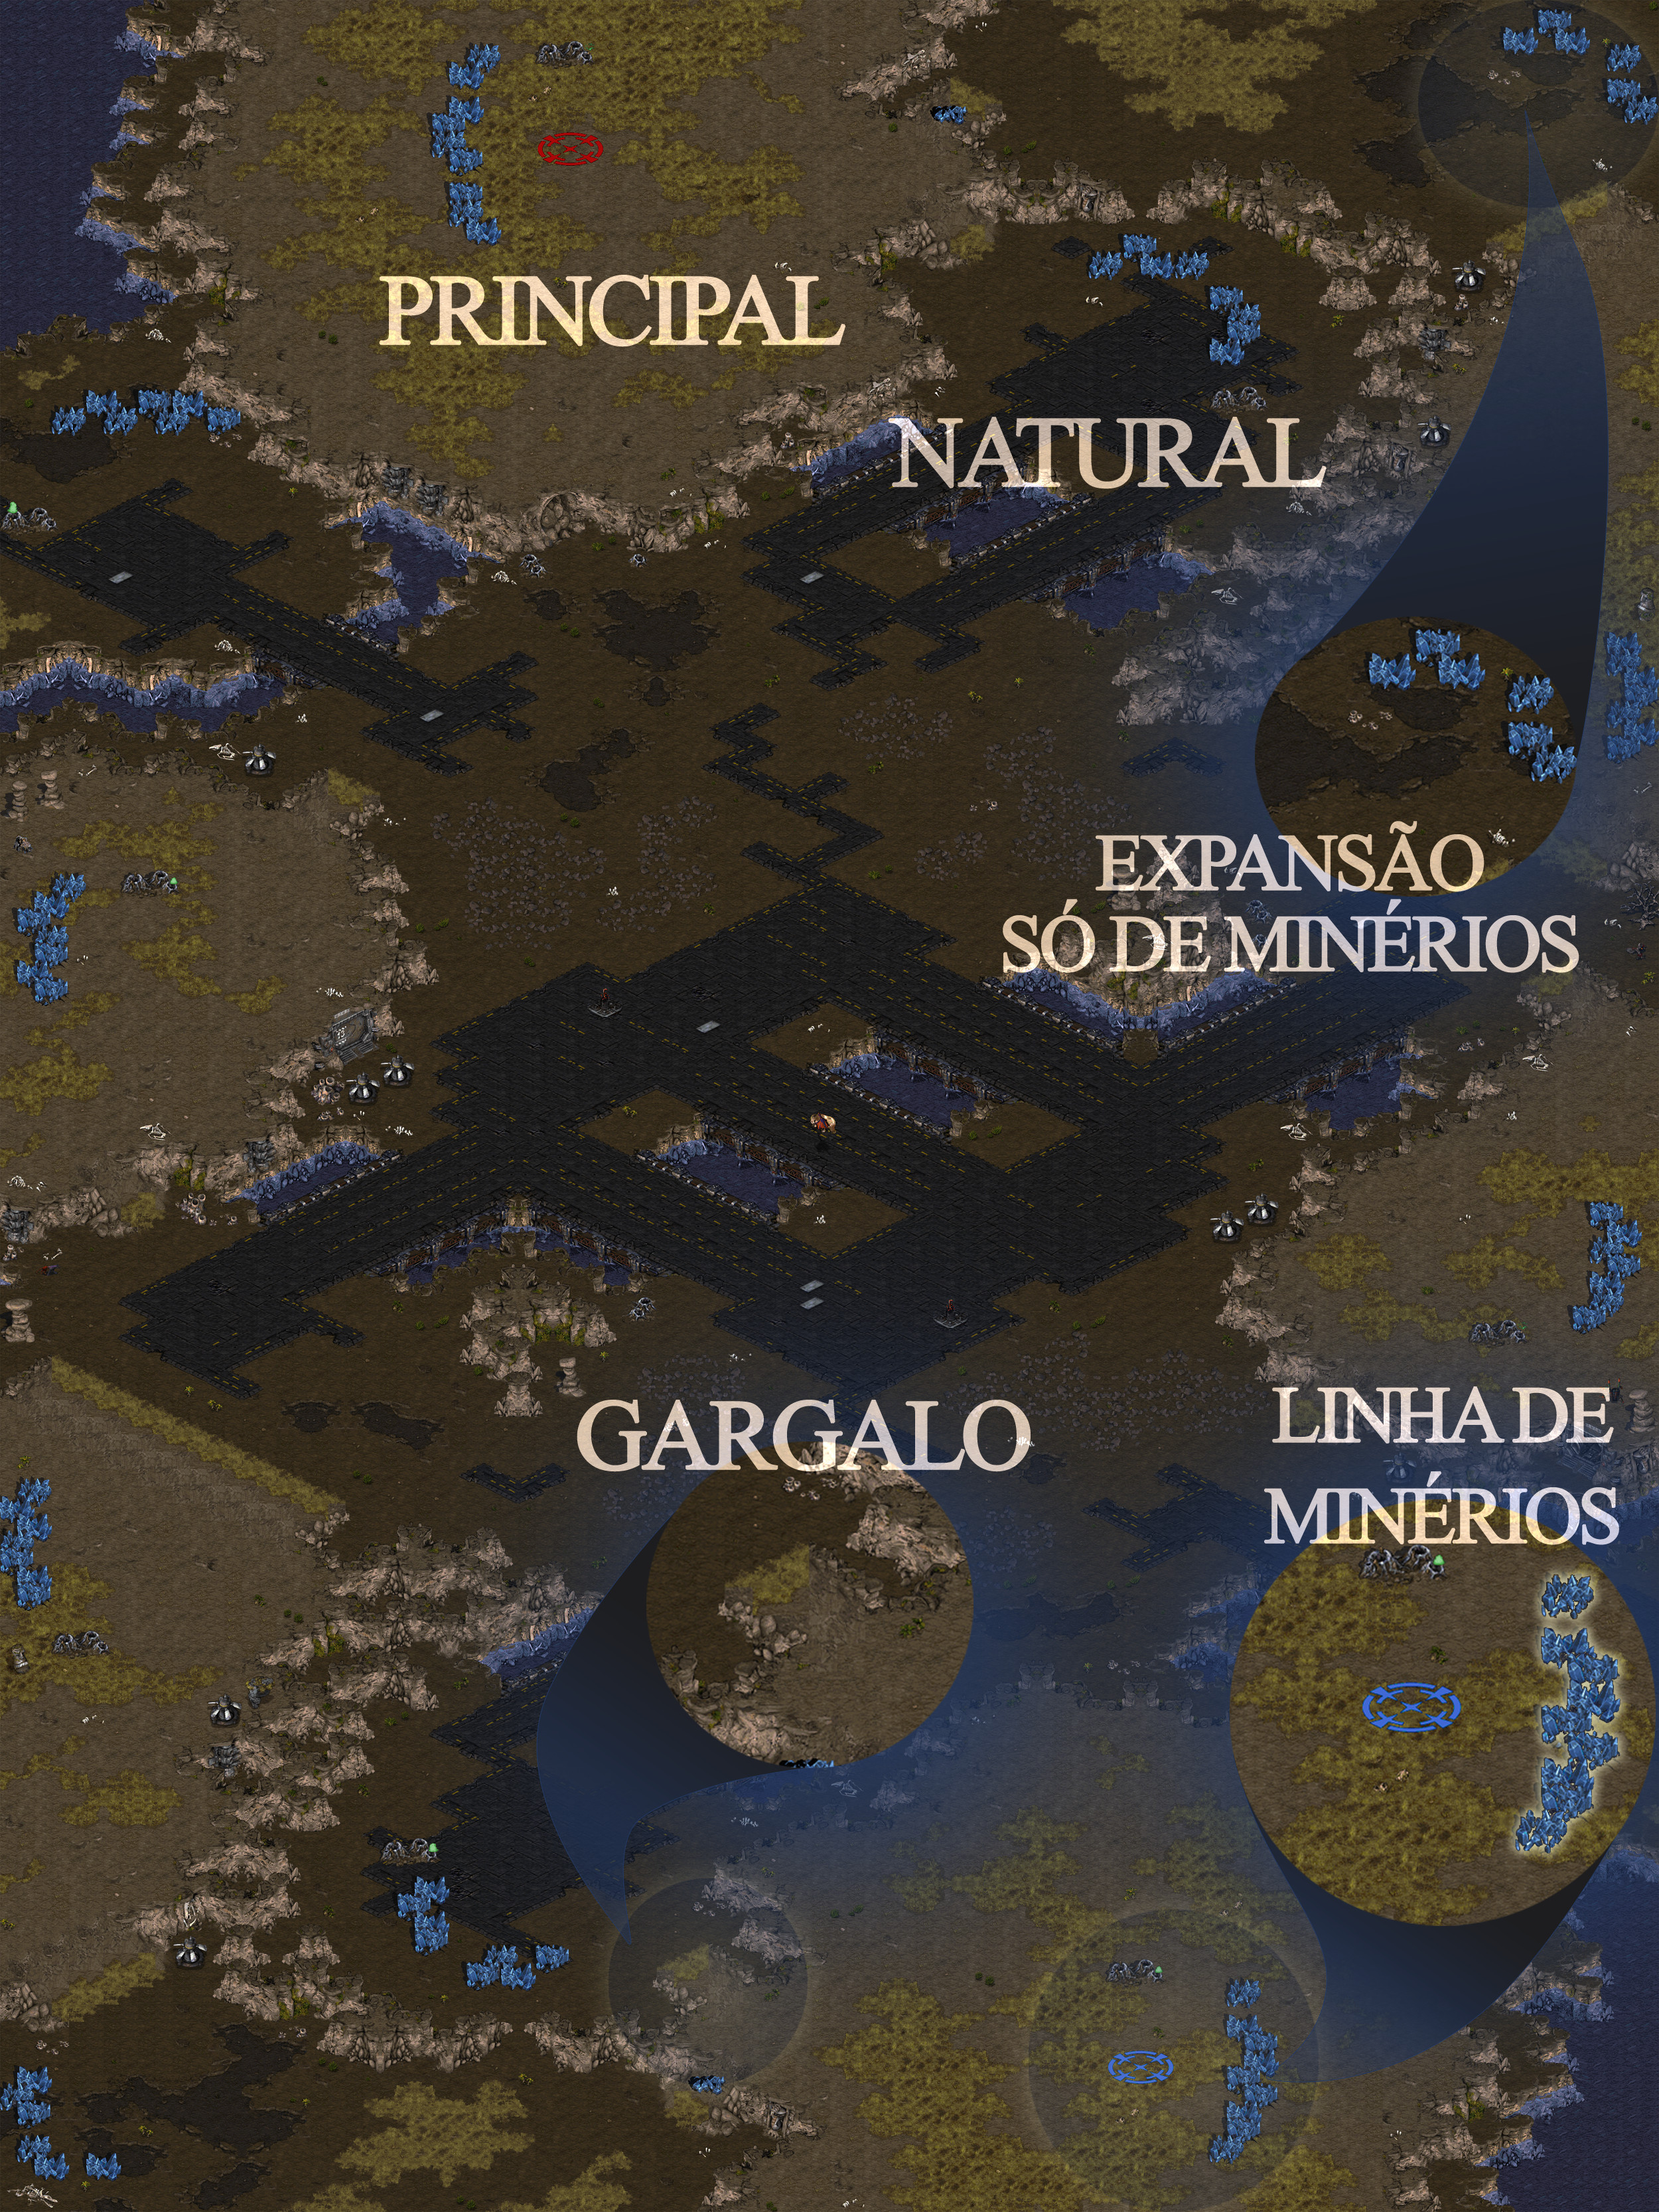
\includegraphics[scale=0.18]{Imagens/mapa-tudo.jpg}
	\caption{Indica��o de base principal e natural, e indica��o do significado dos principais termos no mapa Destination.}
	\label{fig:natural}
\end{figure}

\section{Processo de decis�o nas partidas de StarCraft}
StarCraft � um jogo que fornece pouca informa��o ao jogador sobre o estado atual da partida. O jogador consegue ver apenas aquilo que est� dentro do campo de vis�o de suas unidades. O que est� fora desse campo de vis�o fica coberto pelo que � conhecido como \emph{n�voa de guerra}, em ingl�s \emph{fog of war} ou FOW. Essa n�voa � respons�vel por inserir a incerteza que existe em um ambiente de guerra. O terreno que est� coberto pela FOW pode ter dois estados: desconhecido ou visto recentemente. Posi��es do mapa desconhecidas ficam completamente obscuras, sendo imposs�vel para o jogador saber dentro da partida quais s�o as caracter�sticas do terreno. O terreno j� visitado fica vis�vel para o jogador, por�m com uma tonalidade mais escura para diferenci�-lo do terreno dentro do seu campo de vis�o. Nesse terreno, tamb�m � poss�vel ver a posi��o das estruturas inimigas na �ltima vez que o jogador passou pela regi�o (Figura~\ref{fig:fow}).

\begin{figure}[H]
	\centering
	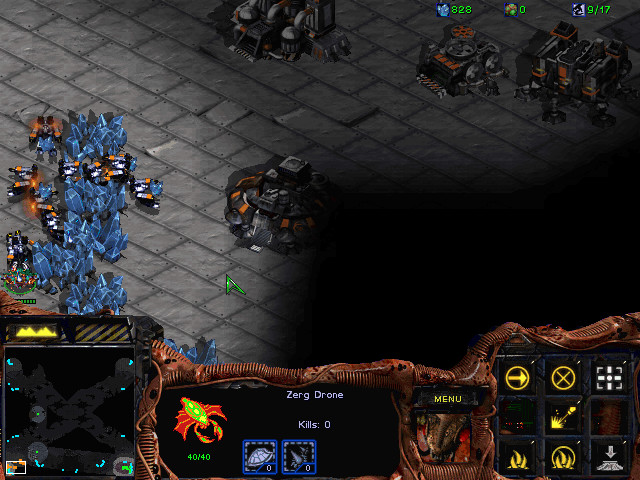
\includegraphics[scale=0.4]{Imagens/fow.jpg}
	\caption[N�voa de guerra em StarCraft.]{N�voa de guerra em StarCraft. No canto esquerdo, em uma tonalidade mais clara, est� uma �rea vis�vel ao jogador. No canto superior direito est� uma �rea recentemente visitada pelo jogador. � poss�vel ver estruturas e a tonalidade � mais escura que a �rea vis�vel. No canto inferior direito est� uma �rea inexplorada. N�o � poss�vel adquirir nenhum tipo de informa��o desta �rea at� que uma unidade a explore.}
	\label{fig:fow}
\end{figure}

Ao iniciar uma partida, o jogador deve se fazer uma s�rie de perguntas a fim de tomar as melhores decis�es:
\begin{enumerate}
	\item Qual a ra�a que estou enfrentando?
	\item Em que mapa estou jogando?
	\item Quais aberturas posso utilizar contra essa ra�a nesse mapa?
	\item Quais aberturas o oponente pode usar?
	\item Onde ele est�?
\end{enumerate}

Respondendo essas perguntas, o jogador poder� tra�ar um plano estrat�gico inicial e come�ar a tentar execut�-lo. Primeiramente, deve coletar recursos com seus trabalhadores. Em StarCraft, n�o h� como mandar seus trabalhadores minerarem diretamente da base antes de cri�-los, como acontece em jogos como Age of Empires. Por isso, o jogador deve lev�-los individualmente ap�s sua cria��o at� uma jazida de min�rios para a coleta. Depois de coletar min�rios e produzir trabalhadores, o jogador precisar� construir estruturas. A posi��o de constru��o das estruturas � escolhida normalmente de acordo com ``a posi��o mais pr�ximo da base'', por�m isso nem sempre � desej�vel, a depender da abertura. Por exemplo, a abertura Protoss de expans�o r�pida, \emph{Forge Fast Expand}, s� � poss�vel com a cria��o de uma muralha de estruturas pr�xima � expans�o (Figura~\ref{fig:ffe}), j� que h� uma grande chance do oponente tentar puni-lo por ter escolhido uma abertura \emph{greedy}.

\begin{figure}[H]
	\centering
	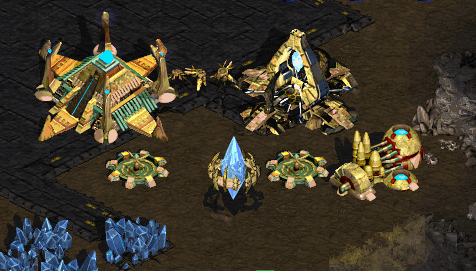
\includegraphics[scale=0.5]{Imagens/PwDestination9.png}
	\caption[Estado da expans�o na abertura Protoss \emph{Forge Fast Expand}.]{Estado da expans�o na abertura Protoss \emph{Forge Fast Expand}. As estruturas e unidades s�o organizadas de forma a dificultar a movimenta��o das unidades inimigas, que podem ser atingidas pelos dois canh�es de f�tons que est�o pr�ximos do pilar energ�tico, a estrutura azul central. Esta organiza��o serve para proteger tanto a base que est� situada na natural como a base principal.}
	\label{fig:ffe}
\end{figure}

Enquanto constr�i estruturas e cria trabalhadores, o jogador deve procurar o seu oponente pelo mapa, sendo importante, para isso, identificar as posi��es iniciais, para ter um direcionamento melhor na sua explora��o. Ap�s encontrar seu oponente, o jogador deve identificar sua abertura e tentar reagir apropriadamente. Por exemplo, caso o oponente tenha iniciado o jogo com um \emph{cheese rush}, o jogador ter� que se focar em defender-se. Ele pode fazer isso construindo estruturas de defesa e unidades militares para ser capaz de defletir o ataque inimigo. Cada abertura pode necessitar de uma rea��o diferente das outras.

No decorrer do jogo, conforme a partida vai evoluindo, perguntas mais complexas v�o aparecendo, como:
\begin{enumerate}
	\item Que abertura o oponente usou de fato?
	\item Que transi��o fa�o, ap�s ver a abertura de meu oponente?
	\item Quando posso expandir?
	\item Onde posso expandir?
	\item Onde colocar estruturas de defesa?
	\item Qual a composi��o de unidades que devo ter?
	\item Quantas estruturas de produ��o devo ter no meio-jogo?
	\item Onde o oponente est� expandindo?
	\item Qual a composi��o do seu ex�rcito?
	\item Que tecnologias pesquisou?
	\item Onde ir� atacar e com que unidades?
	\item Quais tecnologias devo pesquisar?
	\item Quando devo atacar?
	\item Onde devo atacar?
\end{enumerate}

Al�m disso, h� perguntas que n�o dependem do pensamento estrat�gico de mais alto n�vel, sendo mais relacionadas ao controle de ex�rcito:
\begin{enumerate}
	\item Como devo atacar?
	\item Qual deve ser o posicionamento das minhas unidades?
	\item Que unidades inimigas devem ser focadas primeiro em um combate?
	\item Quando devo recuar?
\end{enumerate}

Respondendo essas perguntas de acordo com o metajogo vigente, os jogadores profissionais conseguem determinar as composi��es, rea��es, \emph{timings} e transi��es mais eficientes. O intuito deste trabalho � olhar para o que j� foi feito pelos jogadores profissionais como o resultado de um grande processo de aprendizado e tentar levar esses questionamentos para dentro de um modelo de \emph{game AI}.


	
	% Capitulo 2: Segundo captulo (arquivo Includes/Capitulo2.tex)
	% Cap�tulo 2
\chapter{Modelo organizacional de \emph{game AI} para RTS}

\begin{figure}[ht]
	\centering
	\scalebox{0.7} {
		\begin{tikzpicture}[->, shorten >=1pt,auto,ultra thick]
			\tikzstyle{vertex}=[circle,fill=black!20,minimum size=3cm,node distance=4cm]
			\node[vertex,align=center] (ind) {Ind�stria};
			\node[vertex,fill=black!30,align=center] (head) [above of=ind] {Cerebrate};
			\node[vertex,align=center] (tec) [right of=ind] {Tecnologia};
			\node[vertex,align=center] (inf) [left of=ind] {Infraestrutura};
			\node[vertex,align=center] (min) [below of=inf] {{Minas e}\\Trabalho};
			\node[vertex,fill=black!10,align=center] (eco) [below of=tec] {Economia};
			\node[vertex,align=center] (def) [below of=eco] {Defesa};
			\node[vertex,align=center] (int) [left of=def] {Intelig�ncia};
			\path
				(head) edge [bend left=0] node { } (ind)
				(ind) edge [bend left=0] node { } (min)
				(ind) edge [bend left=10] node { } (inf)
				(inf) edge [bend left=10] node { } (ind)
				(ind) edge [bend left=0] node { } (eco)
				(ind) edge [bend right=10] node { } (def)
				(ind) edge [bend left=0] node { } (int)
				(ind) edge [bend left=10] node { } (tec)
				(tec) edge [bend left=10] node { } (ind)
				(inf) edge [bend left=40] node { } (tec)
				(inf) edge [bend left=0] node { } (min)
				(min) edge [bend left=0] node { } (int)
				(inf) edge [bend left=10] node { } (int)
				(def) edge [bend left=0] node { } (int)
				(tec) edge [bend left=0] node { } (eco)
				(inf) edge [bend left=0] node { } (eco)
				(tec) edge [bend right=10] node { } (int)
				(def) edge [bend left=0] node { } (int)
				(def) edge [bend right=10] node { } (min);
		\end{tikzpicture}
	}
	\caption[Fluxo de comunica��o dos agentes.]{Fluxo de comunica��o dos agentes. As setas apontam do requisitador ao seu alvo. C�rculos escuros indicam os minist�rios que controlam diretamente as unidades dentro do jogo. O c�rculo claro indica que o minist�rio da economia funciona apenas como sensor para os outros minist�rios. O Cerebrate � o conjunto de todos os minist�rios e funciona como o or�culo do minist�rio da ind�stria, dando a abertura a ser usada para ele.}
	\label{fig:modelo}
\end{figure}

Diversos trabalhos foram publicados com o foco em StarCraft e v�rios rob�s foram criados para ele. Por�m, poucos trabalham apresentam um modelo completo de funcionamento de uma \emph{game AI} voltada ao jogo. Um destes � o trabalho de \citeonline{weberm11}. Neste artigo, eles descrevem a arquitetura do EISBot, que fora baseado em um \emph{framework} integrado de agentes para o jogo \emph{Wargus}. Esta arquitetura � composta de cinco gerenciadores que dividem o \emph{gameplay} em subproblemas. O gerenciador de estrat�gias � respons�vel pela sele��o de estrat�gias e pela determina��o de tempos de ataque. O gerenciador de renda controla os trabalhadores, a coleta de recurso e a expans�o econ�mica. O gerenciador de constru��es se responsabiliza pelos pedidos de constru��o de estruturas. O gerenciador t�tico executa as tarefas de combate e os comportamentos de microgerenciamento. E o gerenciador de reconhecimento implementa comportamentos de patrulha.

Foi observado que um agente fica sobrecarregado de tarefas distintas, sendo este o gerenciador de estrat�gias. Este agente deve modelar o oponente, inferir estrat�gias e definir os tempos de ataque da \emph{game AI}. Para propor um novo modelo mais distribu�do, observamos a divis�o de tarefas de gerenciamento feita pelos governos atuais. Eles s�o compostos por minist�rios, que se encarregam de gerenciar atividades distintas, por�m interdependentes, de um pa�s. Para este trabalho foram escolhidos seis minist�rios e uma Ag�ncia de Intelig�ncia, que apesar de n�o ser um minist�rio de fato, � uma entidade cuja �rea de trabalho � independente das �reas dos minist�rios e que os servi�os deles dependem da sua atua��o. Os minist�rios escolhidos est�o brevemente descritos na Tabela~\ref{tab:departments} e suas intera��es est�o expostas na Figura~\ref{fig:modelo}.

\begin{table}[h]
	% T�tulo de tabelas sempre aparecem antes da tabela
	\center
	{
		\begin{tabular}{l|l}
			\hline
			\textbf{Departamento}						 & \textbf{Responsabilidade}\\
			\hline
			Minist�rio de Minas e do Trabalho			 & Administra��o dos trabalhadores\\
			Minist�rio da Economia						 & Monitoramento dos recursos\\
			Minist�rio de Infraestrutura				 & Constru��o de estruturas\\
			Minist�rio da Ind�stria						 & Administra��o da ordem de constru��o\\
			Minist�rio da Defesa						 & Administra��o do ex�rcito\\
			Minist�rio de Tecnologia					 & Pesquisa de novas tecnologias\\
			Ag�ncia de Intelig�ncia Militar & Coletar dados do jogador inimigo\\
			\hline
		\end{tabular}
	}
	\caption{Agentes do sistema e suas responsabilidades}
	\label{tab:departments}
\end{table}

Como jogos de estrat�gia em tempo real possuem fases, este modelo tamb�m foi modelado para incorporar estas fases no desenrolar das partidas. O modelo proposto possui duas etapas de funcionamento: \emph{a��o} e \emph{rea��o}. Elas s�o espelhadas nos conceitos existentes de abertura e meio-jogo. A a��o � a fase em que uma abertura � escolhida e executada. A escolha de aberturas se d� por um produto da an�lise do mapa com um fator aleat�rio inicial, a passividade da intelig�ncia artificial.

Na fase de a��o, a \emph{game AI} verifica as possibilidades referentes �s aberturas que podem ser escolhidas no in�cio do jogo. Essas aberturas s�o selecionadas previamente, a partir das estrat�gias mais conhecidas, e classificadas de acordo com o grau de agressividade e com a seguran�a que existe ao execut�-las de acordo com um dos tipos de dist�ncias: (a) dist�ncia terrestre entre as principais, (b) dist�ncia a�rea entre as principais.

Para classificar as estrat�gias desta maneira, cria-se duas fun��es de pertin�ncia referentes a cada uma das aberturas, uma para a dist�ncia � qual est� relacionada e outra para a agressividade. A sele��o de quais aberturas poder�o ser utilzadas pelo sistema e a cria��o de suas respectivas fun��es devem ser feitas previamente, no estudo de caso do modelo para o jogo escolhido. As fun��es relacionadas �s aberturas devem ser modeladas com o aux�lio de algum especialista no jogo. A escolha da abertura numa partida � feita baseando-se ent�o nas combina��es das fun��es de pertin�ncia e, a partir delas, escolhe-se aleatoriamente uma entre as duas maiores.

Durante a fase de a��o, o sistema apenas executar� a abertura, que � uma ordem de constru��o. Assim, apenas as funcionalidades dos minist�rios extritamente necess�rias ser�o utilizadas durante essa fase.

Ap�s a execu��o da abertura, a intelig�ncia artificial passa para a outra fase da execu��o, a rea��o. Nesta fase, os minist�rios ativam as funcionalidades que estavam dormentes durante a fase anterior. Os minist�rios coletam dados referentes �s suas responsabilidades e procuram agir com o foco de expandir-se economicamente e reagir aos movimentos do oponente. Essa expans�o se dar� com a constru��o de novas bases em locais estrat�gicos do mapa, al�m da produ��o de um ex�rcito e de estruturas de defesa que consigam proteger efetivamente todas as bases. Como todas as principais possuem uma natural, esta � a primeira escolha de expans�o. A partir dela, o processo de decis�o passa a ser mais complexo, sendo necess�ria a cria��o de uma fun��o que consiga expressar as motiva��es de um jogador humano ao escolher tais expans�es.

Para facilitar a cria��o de um m�todo que reaja a um grupo de unidades inimigas, s�o designados pap�is para as unidades (tabela~\ref{tab:roles}) de forma que, quando a \emph{game AI} detecta uma unidade que cumpra um determinado papel no ex�rcito inimigo, comece a produzir unidades que combatem efetivamente este papel. Os pap�is das unidades s�o usados pelo minist�rio da defesa e pela ag�ncia de intelig�ncia.
\begin{table}[h]
	% T�tulo de tabelas sempre aparecem antes da tabela
	\center
	{
		\begin{tabular}{l|l}
			\hline
			\textbf{Papel}			& \textbf{Significado}\\
			\hline
			\emph{Large-scale}		& Unidades que formam o n�cleo do ex�rcito\\
			\emph{Anti-air}			& Unidades que atacam unidades a�reas\\
			\emph{Harass}			& Unidades r�pidas e com poucos pontos de vida\\
			\emph{Area of Effect}	& Unidades que causam dano em �rea\\
			\emph{Siege}			& Unidades que possuem longo alcance\\
			\emph{Caster}			& Unidades que possuem habilidades especiais ofensivas\\
			\emph{Stealth}			& Unidades que podem ficar invis�veis\\
			\emph{Air}				& Unidades a�reas\\
			\emph{Tank}				& Unidades que possuem alta durabilidade\\
			\emph{Detector}			& Unidades que exp�em unidades invis�veis\\
			\emph{Transport}		& Unidades de transporte\\
			\emph{No Ground Attack}	& Unidades a�reas incapazes de atacar unidades terrestres\\
			\hline
		\end{tabular}
	}
	\caption{Pap�is das unidades}
	\label{tab:roles}
\end{table}


\section{Minist�rio de Minas e do Trabalho}
O minist�rio de minas tem como fun��es:
\begin{itemize}
	\item Manter os trabalhadores minerando;
	\item Manter a satura��o de trabalhadores das bases em n�veis adequados.
\end{itemize}

\subsection{Atua��o dos mineradores}
J� que o principal foco do minist�rio � fazer os trabalhadores minerarem, o agente deve fazer uma rela��o dos recursos dispon�veis nas bases ocupadas pelo jogador com os seus trabalhadores. Cada recurso deve possuir uma \emph{flag} que ativa quando h� um trabalhador minerando e desativa caso n�o haja. Esse atributo servir� para definir os estados dos outros trabalhadores.

\begin{figure}[h]
	\centering
	\scalebox{0.8} {
		\begin{tikzpicture}[->,shorten >=1pt,auto,thick]
			\tikzstyle{vertex}=[circle,fill=black!25,minimum size=3cm,node distance=5cm]
			\node[vertex,fill=white,minimum size=0cm] (start) { };
			\node[vertex,align=center,node distance=2.2cm] (a) [right of=start] {\textbf{Esperando}};
			\node[vertex,align=center] (b) [right of=a] {Minerando};
			\node[vertex,align=center] (c) [right of=b] {Retornando};
			\path
				(start) edge [bend left=0] node { } (a)
				(a) edge [bend left=40] node {\footnotesize{Jazida livre}} (b)
				(b) edge [bend left=40] node {\footnotesize{Min�rio em m�os}} (c)
				(c) edge [bend left=30] node {\footnotesize{Sem min�rio}} (a);
		\end{tikzpicture}
	}
	\caption{M�quina de estados dos mineradores}
	\label{fig:minestate}
\end{figure}

Al�m disso, cada campo de min�rios deve ter no m�ximo um n�mero $S$ de trabalhadores, que revezam na execu��o da tarefa. Enquanto um deles retorna com o min�rio que coletou, o outro come�a a minerar. Este trabalho � feito com uma m�quina de tr�s estados (Figura~\ref{fig:minestate}) para cada trabalhador:

\begin{itemize}
	\item \textbf{Esperando}: estado inicial dos trabalhadores, no qual ele espera at� que a jazida � qual ele est� relacionado esteja livre.
	\item \textbf{Minerando}: estado no qual o trabalhador ativa a \emph{flag} de ocupado do campo e come�a a miner�-lo.
	\item \textbf{Retornando}: nesse estado, o trabalhador desativa a \emph{flag} e retorna o min�rio para a estrutura de coleta de recursos.
\end{itemize}

\subsection{Remanejamento dos trabalhadores}
Em StarCraft, o jogador come�a o jogo com uma base e quatro trabalhadores e, caso deseje partir para um jogo longo, deve progredir de forma a expandir sua economia com a constru��o de novas bases e mais trabalhadores. Cada uma das bases, por sua vez, possui uma quantidade de jazidas de min�rios. Devido �s caracter�sticas do jogo, essas jazidas podem ser mineradas de maneira �tima com 2 ou 3 trabalhadores por jazida.

Al�m disso, o jogador advers�rio possui um ex�rcito que pode estar se movimentando pelo mapa, podendo aproximar-se de alguma base. Esse movimento aumenta ou diminui o risco correspondente � minera��o de uma base conforme o ex�rcito se aproxima ou se afasta dessa base, respectivamente.

Com a cria��o de uma nova base, a exaust�o de uma jazida de min�rios ou um risco elevado em alguma base j� estabelecida, � necess�rio transferir trabalhadores entre as bases a fim de aumentar a renda de min�rios. Por�m essa transfer�ncia acarreta em uma perda tempor�ria de lucro, sendo necess�rio, portanto, minimizar essa perda.

Esse problema foi modelado da seguinte forma: dados um ponto de satura��o S; um conjunto de bases $B = \{1, ... , n\}$, onde cada base $i$ possui uma quantidade de trabalhadores $w_i$, uma quantidade de jazidas de min�rios $m_i$ e um risco $r_i$; e uma matriz de dist�ncias $D_{n,n}$ que cont�m as informa��es das dist�ncias entre as bases, a solu��o se d� em uma matriz $T_{n,n}$, tal que cada elemento $t_{ij}$ informa quantos trabalhadores ir�o da base $i$ � base $j$.

Essa solu��o deve obedecer a duas restri��es: nenhuma base pode transferir mais trabalhadores que a quantidade inicial, isto �, a soma de uma linha qualquer $T_i$ deve ser igual a $w_i$, e nenhuma base pode transferir trabalhadores para uma base que esteja trabalhando no seu limite de satura��o, $S m_i$. Isto significa que bases podem ficar com mais trabalhadores que podem comportar se n�o houver nenhuma op��o para onde mandar o excesso. A partir disso, deve-se procurar minimizar a soma das dist�ncias percorridas por cada um dos trabalhadores, ao mesmo tempo que deve-se minimizar a soma dos riscos correspondentes � minera��o em todas as bases ap�s a transfer�ncia.

De forma mais formal, o problema constitui em:
\begin{equation*}
	\displaystyle
	\begin{array}{l l}
		\text{Minimizar } & \quad \text{custo}(x) = \mathlarger{\sum}_{i = 1}^n \mathlarger{\sum}_{j = 1}^n t_{ij}d_{ij} + \lambda\left(\mathlarger{\sum}_{j = 1}^n \text{max}\left\{0,\mathlarger{\sum}_{i = 1}^nt_{ij} - S m_i\right\}\right)\\
		\text{Minimizar } & \quad \text{risco}(x) = \mathlarger{\sum}_{j = 1}^n r_j \mathlarger{\sum}_{i = 1}^n  t_{ij}\\
		\text{Sujeito a:} & \quad\\
		&\mathlarger{\sum}_{j = 1}^n t_{ij} = w_i, \forall i \in \{1, ... , n\}\\
		&\left\{
			\begin{array}{l l}
				\mathlarger{\sum}_{i = 1}^n t_{ij} - t_{jj} = 0 & \quad, t_{jj} \geq S m_j \\
				\mathlarger{\sum}_{i = 1}^n t_{ij} \leq S m_j& \quad , t_{jj} < S m_j
			\end{array}
			, \forall j \in \{1, ... , n\}
		\right.\\
		&t_{ij} \in \mathbb{N}_0, \forall i,j \in \{1, ... , n\}
	\end{array}
\end{equation*}

Onde $\lambda$ � a penalidade por trabalhador que uma base recebe por estar operando al�m de sua capacidade, ap�s a transfer�ncia.

Apesar do modelo de remanejamento ter sido criado com um foco em StarCraft, ele pode ser aplicado em outros RTS que possuam um paradigma que comporte a ideia de um conjunto de coletores em uma localiza��o recoltando um tipo de recurso, como Age of Empires.

\section{Minist�rio da Economia}
A fun��o do minist�rio da economia � monitorar os gastos e a renda do jogador. Para isso, ele precisa saber a renda m�dia dos �ltimos \emph{frames} e os gastos previstos para cada estrutura de cria��o de unidades.

Al�m disso, ele precisa manter um controle sobre o que est� sendo reservado para alguma produ��o, como estruturas ou tecnologias. Esses gastos devem entrar em uma lista de or�amentos e sair�o quando o projeto do or�amento for iniciado. Como o minist�rio precisa informar que existem gastos enfileirados, os outros agentes precisam pedir a informa��o sobre os recursos atuais ao minist�rio da economia, ao inv�s de olhar diretamente nos recursos do jogador.

\section{Minist�rio de Infraestrutura}
As fun��es do minist�rio de infraestrutura s�o:
\begin{itemize}
	\item Posicionar as futuras estruturas.
	\item Selecionar trabalhadores e mandar construir as estruturas necess�rias.
\end{itemize}

Similarmente ao minist�rio de minas, o minist�rio de infraestrutura recebe o controle de trabalhadores que ir�o construir as estruturas solicitadas pela ordem de constru��o e atribui a eles uma m�quina de estados finita, por�m antes precisa posicionar a futura estrutura em um lugar prop�cio. Ap�s a constru��o, caso seja uma estrutura de cria��o de unidades, o minist�rio as guarda em um conjunto separado para cada tipo de estrutura.

\subsection{Atua��o dos construtores}
O funcionamento dessa m�quina de estados finita � semelhante � m�quina dos mineradores. Por�m, ao contr�rio destes, os construtores devem ter medo de unidades militares inimigas. Eles devem cancelar a constru��o quando virem que est�o sob ataque, pois, na maioria dos RTS, cancelar a constru��o de uma estrutura retorna parte da quantia gasta.

A cada construtor s�o atribu�dos uma estrutura e um local de constru��o. Essas informa��es s�o guardadas para que o construtor saiba aonde deve ir, e para que o minist�rio consiga saber quais estruturas foram canceladas ou destru�das e possa fazer um pedido de reconstru��o ao minist�rio da ind�stria.

\begin{figure}[h]
	\centering
	\scalebox{0.8} {
		\begin{tikzpicture}[->,shorten >=1pt,auto,thick]
			\tikzstyle{vertex}=[circle,fill=black!25,minimum size=2.5cm,node distance=5cm]
			\node[vertex,fill=white,minimum size=0cm] (start) { };
			\node[vertex,align=center,node distance=2.2cm] (a) [right of=start] {Movendo};
			\node[vertex,align=center] (b) [right of=a] {Construindo};
			\node[vertex,align=center] (c) [below of=a] {Fugindo};
			\node[vertex,align=center] (d) [below of=b] {\textbf{Terminado}};
			\path
				(start) edge [bend left=0] node { } (a)
				(a) edge [bend left=40] node {\footnotesize{Na posi��o de constru��o}} (b)
				(a) edge [bend left=15] node {\footnotesize{Sendo atacado}} (c)
				(b) edge [bend left=15] node {\footnotesize{Sendo atacado}} (c)
				(c) edge [bend left=15] node {\footnotesize{Fora de perigo}} (a)
				(b) edge [bend left=20] node {\footnotesize{Constru��o conclu�da}} (d);
		\end{tikzpicture}
	}
	\caption{M�quina de estados dos construtores}
	\label{fig:buildstate}
\end{figure}

Al�m disso, os construtores executam seu trabalho seguindo uma m�quina de estados finita (Figura~\ref{fig:buildstate}) com os seguintes estados:

\begin{itemize}
	\item \textbf{Movendo}: estado inicial dos construtores, no qual ele move-se at� o local de constru��o.
	\item \textbf{Construindo}: estado no qual o construtor est� a construir sua estrutura.
	\item \textbf{Fugindo}: nesse estado, o construtor cancela qualquer ordem que tinha e procura fugir dos atacantes.
	\item \textbf{Terminado}: aqui, o construtor � dispensado do servi�o, podendo voltar � coleta de recursos. O minist�rio de infraestrutura mant�m, entretanto, a estrutura constru�da.
\end{itemize}

\subsection{Posicionamento de estruturas}
Os mapas da maior parte dos jogos de estrat�gia em tempo real s�o representados como grades, onde cada bloco dessa grade pode ser chamado de bloco de constru��o e estruturas possuem uma certa �rea que ocupam nessa grade. Al�m dessa grade, h� tamb�m uma grade com maior precis�o que modela o espa�o de movimenta��o dos personagens no mapa. Essas duas representa��es podem ser observadas em jogos como Age of Empires e StarCraft.

Para avaliar o posicionamento de uma estrutura, ser� utilizado um novo m�todo que utiliza o conceito de campos potenciais (\emph{potential fields}), que foram usados com sucesso em v�rios jogos para resolver problemas de \emph{pathfinding} \cite{sajjad11} \cite{hagelback12}. Essa t�cnica se baseia em atribuir \emph{cargas} a alguns elementos do jogo de forma que esses elementos podem ser atrativos ou repulsivos. Ao colocar uma carga atrativa no destino de uma unidade e carga repulsiva nos obst�culos, por exemplo, � poss�vel fazer um m�todo simples que consegue chegar ao destino evitando os obst�culos. O uso dessa t�cnica para determinar o posicionamento de estruturas necessita de uma pequena mudan�a na mentalidade, pois o destino ainda n�o � conhecido.

Dependendo de cada jogo, os elementos que receberiam carga variam. Em jogos como Age of Empires e StarCraft, o posicionamento das estruturas vai depender se haver� ou n�o necessidade de cria��o de uma muralha de estruturas para impedir o movimento das unidades inimigas em algum gargalo. Em Age of Empires 2, � comum a cria��o de muralhas em gargalos criados por florestas, especialmente gargalos que funcionam como potenciais ``portas dos fundos''. Em StarCraft, essa abordagem � usada tamb�m por cada ra�a, mas em situa��es diferentes. Os Protoss fazem uma muralha em sua base a fim de impossibilitar a destrui��o de uma expans�o r�pida e a passagem de unidades inimigas pela sua natural sem que levem algum tipo de retalia��o; os Terran o fazem para defender sua base principal de \emph{rushes} Zerg, impedindo parcialmente ou completamente a passagem de unidades; e os Zerg o fazem com o mesmo intuito dos Protoss, apenas em um per�odo mais tardio dentro do jogo.

Como visto nas figuras~\ref{fig:aoewall} e~\ref{fig:scbwwall}, a posi��o das estruturas em muralhas tende a se aproximar da regi�o perif�rica da base, ou de algum gargalo, como � o caso das muralhas dos Terran. Isso implica em dizer que, para a cria��o de muralhas, as bordas s�o atrativas, ent�o devem receber carga equivalente.

Por�m, ao analisar o posicionamento de estruturas que n�o fazem parte de muralhas, � poss�vel perceber que h� uma repuls�o por gargalos, j� que elas devem oferecer espa�o livre para as unidades navegarem. Algumas vezes, como o caso dos Terran em StarCraft, h� uma repuls�o at� mesmo por outras estruturas, uma vez que o espa�o entre elas pode impedir as unidades de navegar. Al�m disso, recursos naturais repelem estruturas, pois as estruturas n�o podem impedir os trabalhadores de colet�-lo. Essas caracter�sticas devem ser quantificadas e verificadas de acordo com o jogo em quest�o. Em Age of Empires 2, a dist�ncia entre um recurso e a estrutura de entrega de recurso (como uma \emph{town center}) normalmente � m�nima, sendo necess�rio um valor baixo para a carga de recursos, mas em StarCraft a dist�ncia m�nima entre recurso e base (a �nica estrutura de entrega de recursos do jogo) � alta e pode comportar estruturas grandes dentro dessa brecha, o que implica um valor alto para a carga dos recursos.

\begin{figure}[h]
	\centering
	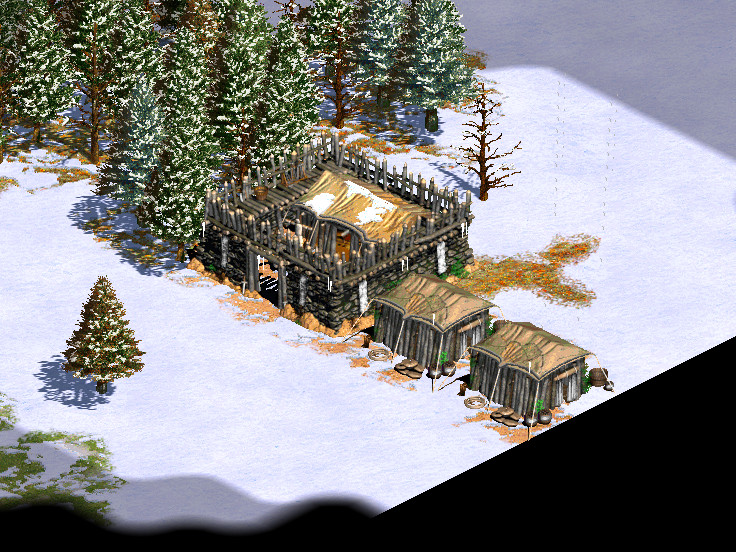
\includegraphics[scale=0.35]{Imagens/aoe-wall.jpg}
	\caption{Exemplo de muralha em Age of Empires}
	\label{fig:aoewall}
\end{figure}

\begin{figure}[H]
	\centering
	\subfloat[Muralha Protoss]{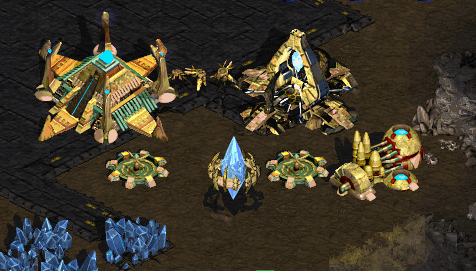
\includegraphics[scale=0.45]{Imagens/PwDestination9.png}}
	\qquad
	\subfloat[Muralha Terran] {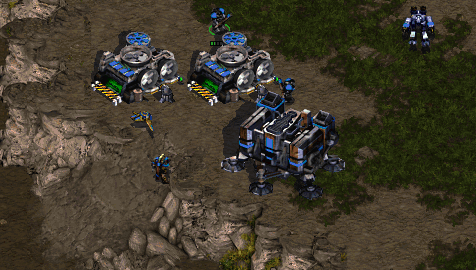
\includegraphics[scale=0.45]{Imagens/TwPython1.png}}
	\qquad
	\subfloat[Muralha Zerg] {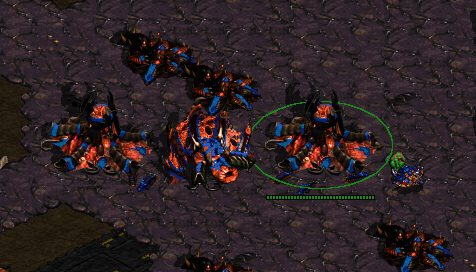
\includegraphics[scale=0.45]{Imagens/ZwDestination12.png}}
	\caption{Muralhas de cada ra�a de StarCraft}
	\label{fig:scbwwall}
\end{figure}

Algumas estruturas tamb�m podem fugir de todos esses conceitos, como estruturas de suprimentos. Elas, quando n�o est�o em posi��es de muralha, est�o em lugares distantes de gargalos e poss�veis focos de ataque, j� que representam tamb�m um outro recurso dentro do jogo. Isso implica que ao posicionar estruturas de suprimentos, dever�o ser utilizados outros valores para cada um dos elementos que podem receber carga.

Como h� duas maneiras distintas de posicionar estruturas, a op��o escolhida procura preencher primeiramente as muralhas, e, somente em seguida, posiciona as estruturas de forma mais tradicional.

Al�m de tentar achar o posicionamento das estruturas da muralha, outra coisa que deve ser considerada � o espa�amento entre as estruturas. Em StarCraft, todas as estruturas possuem tamanho de constru��o e tamanho real, isto �, o tamanho que a estrutura ocupa na grade de constru��o, e outro tamanho na grade de movimenta��o. A partir desses tamanhos � poss�vel calcular a brecha que existe em cada um dos lados de uma estrutura, como pode ser visto na Figura~\ref{fig:gap}. Brechas negativas significam, entretanto, que a estrutura bloqueia a passagem de uma regi�o al�m do seus limites.

\begin{figure}[H]
	\centering
	\subfloat[Constru��es Protoss]{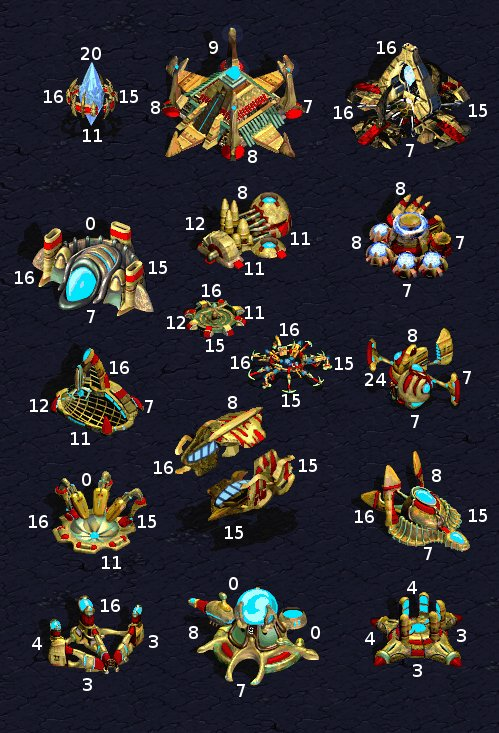
\includegraphics[scale=0.35]{Imagens/Protoss_buildings_gaps.jpg}}
	\qquad
	\subfloat[Constru��es Terran] {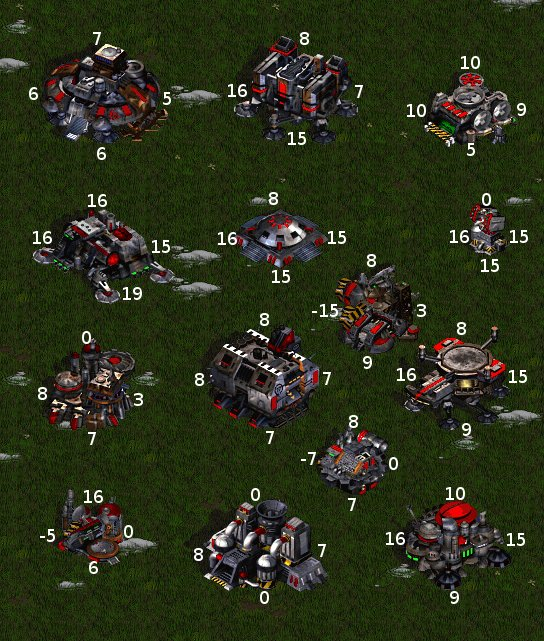
\includegraphics[scale=0.35]{Imagens/Terran_buildings_gaps.jpg}}
	\qquad
	\subfloat[Constru��es Zerg] {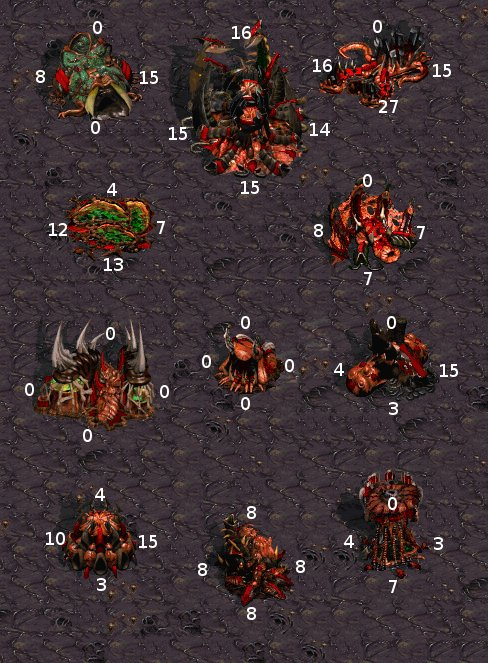
\includegraphics[scale=0.35]{Imagens/Zerg_buildings_gaps.jpg}}
	\caption{Brechas dentro das estruturas de cada ra�a de StarCraft}
	\label{fig:gap}
\end{figure}

\citeonline{certicky13} prop�s uma abordagem para a cria��o de muralhas usando \emph{answer-set programming}, por�m ela requer que sejam dadas de antem�o as estruturas a serem usadas na muralha. Essa abordagem busca reduzir as brechas existentes entre as constru��es.

Al�m do posicionamento e do espa�amento entre estruturas, pode ser levado em conta o custo de cada estrutura.

\section{Minist�rio da Ind�stria}
As fun��es do minist�rio da ind�stria s�o:
\begin{itemize}
	\item Executar a abertura escolhida.
	\item Criar ordens de constru��o no decorrer do jogo.
	\item Guardar todas as estruturas de cria��o de unidades.
\end{itemize}

O minist�rio da ind�stria � respons�vel pela manuten��o da ordem de constru��o da IA. Ele inicialmente ir� receber a ordem de constru��o inicial, isto �, a abertura, de um or�culo. Para a execu��o dessa ordem de constru��o, o minist�rio d� ordens aos minist�rios de infraestrutura e de tecnologia de forma que eles criem as estruturas e pesquisem as tecnologias necess�rias, bem como d� ordens �s estruturas de produ��o, as quais fazem parte de suas responsabilidades.

Ap�s o t�rmino da abertura, o minist�rio da ind�stria come�a a pedir dos outros minist�rios quais as necessidades que eles possuem no momento, e pondera sobre essas necessidades e as capacidades de produ��o da IA para determinar quais passos devem ser tomados a seguir. Ele deve ser capaz de identificar os requisitos de constru��o de unidades e tecnologias, para que n�o fique estagnado tanto tecnologicamente como militarmente.

Para a ordem de constru��o � usada uma fila de prioridades, de forma que o minist�rio tenha como avaliar e implantar mudan�as nesta fila de acordo com as prioridades do estado atual do jogo.

\section{Minist�rio da Defesa}
As fun��es do minist�rio da defesa s�o:
\begin{itemize}
	\item Controlar as unidades militares.
	\item Manter um controle das unidades que pode-se criar e definir uma composi��o ideal a partir disso.
\end{itemize}

\subsection{Controle de unidades}
O controle de unidades foi alvo de in�meros trabalhos ao longo dos anos. Por exemplo, \citeonline{uriarte12} mostraram como criar o comportamento de ``atacar e correr'' usando mapas de influ�ncia. \citeonline{cadena11} e \citeonline{synn12} usaram \emph{case-based reasoning} para o planejamento t�tico. Este agente, ent�o, deve utilizar alguma t�cnica, j� pesquisada ou n�o, para controlar de forma eficiente as unidades militares do jogador.

\subsection{Composi��o de unidades}
A composi��o das unidades deve ser planejada de acordo com o que � poss�vel produzir, levando em considera��o a composi��o do ex�rcito inimigo. Para atingir este feito, dois agentes v�o cuidar de cada aspecto separadamente. A composi��o final vai ficar decidida pelo Minist�rio da Ind�stria, que far� uma negocia��o sobre quais unidades ser�o criadas.

O Minist�rio da Defesa � respons�vel por determinar quais unidades devem ser feitas, sob a �tica do que � poss�vel fazer. A Ag�ncia de Intelig�ncia � encarregada por verificar a composi��o que melhor enfrenta o ex�rcito inimigo. Para esses agentes verificarem isso, eles devem observar os pap�is das unidades e selecionar aquelas que melhor se encaixam na composi��o.

Por exemplo, um jogador Zerg ao enfrentar um oponente Terran pode recorrer a uma composi��o de fim de jogo com zerglings e \emph{ultralisks}\footnote{Unidade zerg do mais alto n�vel tecnol�gico. Unidade militar corpo-a-corpo, com alta durabilidade e dano.}. O jogador Terran pode, ent�o, escolher uma das seguintes alternativas para enfrentar essa composi��o: (a) criar \emph{siege tanks}\footnote{Unidade militar mec�nica terran que possui dois modos de ataque, um com baixo dano contra uma �nica unidade e outro com alto dano em �rea.} para causar uma grande quantidade de dano em �rea tanto nos zerglings, provavelmente matando v�rios de uma s� vez, como nos ultralisks; (b) criar \emph{vultures}\footnote{Unidade militar mec�nica terran de ass�dio. Possui, ap�s pesquisa tecnol�gica, habilidade de depositar \emph{spider mines} que causam grande dano em �rea.} que podem depositar \emph{spider mines} no ch�o, e estas causam tamb�m dano em �rea; (c) criar \emph{science vessels}\footnote{Unidade terran conjuradora e voadora. Amplamente utilizada nos confrontos Terran vs Protoss e Terran vs Zerg.} que podem usar a habilidade \emph{irradiate} e matar ultralisks, deixando o trabalho das unidades militares mais f�cil.

Neste exemplo, suponhamos que o jogador terran n�o possui a capacidade de produzir \emph{siege tanks} ou \emph{science vessels}, e pode produzir tanto \emph{vultures} como \emph{marines}\footnote{Primeira unidade militar biol�gica terran dispon�vel.}. Ent�o, durante a fase de negocia��o, o Minist�rio da Defesa iria propor a cria��o de \emph{vultures} e \emph{marines}, pois os primeiros possuem um bom ataque terrestre contra unidades leves e a habilidade de causar dano em �rea, enquanto os �ltimos possuem maior dano por unidade de tempo, al�m de atacarem unidades a�reas. A Ag�ncia de Intelig�ncia proporia tanto \emph{vultures} como as unidades que o jogador � incapaz de construir, \emph{siege tanks} e \emph{science vessels}, pois elas s�o as que melhor combatem a composi��o inimiga. Isso levaria a intelig�ncia artificial a produzir mais \emph{vultures} do que \emph{marines}, tendendo a ter uma composi��o boa contra as unidades inimigas e consistente entre si.

\section{Minist�rio de Tecnologia}
A fun��o do minist�rio � tirar o jogador de uma estagna��o tecnol�gica, verificando com a Ag�ncia de Intelig�ncia quais tecnologias o oponente j� pesquisou e guardando informa��es sobre as unidades que est�o sendo usadas pelo jogador. 

Tecnologias s�o classificadas de acordo com o papel que eles desbloqueiam nas unidades, seguindo o mesmo exemplo de unidades. A diferen�a sendo que tecnologias podem aprimorar a efetividade de algumas unidades, e isso requer um novo papel, al�m daqueles descritos para as unidades.

Al�m disso, o minist�rio ter� que identificar pr�-requisitos tecnol�gicos para poder guiar corretamente o andamento da \emph{game AI}. Assim, o Minist�rio da Ind�stria poder� perceber que um determinado pr�-requisito est� sendo mais necess�rio do que o esperado e adiantar, se poss�vel, sua posi��o na fila de produ��o.

\section{Ag�ncia de Intelig�ncia Militar}
A ag�ncia de intelig�ncia tem como fun��es:
\begin{itemize}
	\item Analisar o mapa;
	\item Verificar as movimenta��es do ex�rcito inimigo e predizer ataques iminentes;
	\item Verificar e guardar informa��es sobre o desenvolvimento estrat�gico do inimigo.
\end{itemize}

\subsection{An�lise do mapa}

\begin{figure}[htb]
	\centering
	\subfloat[Grafo das bases]{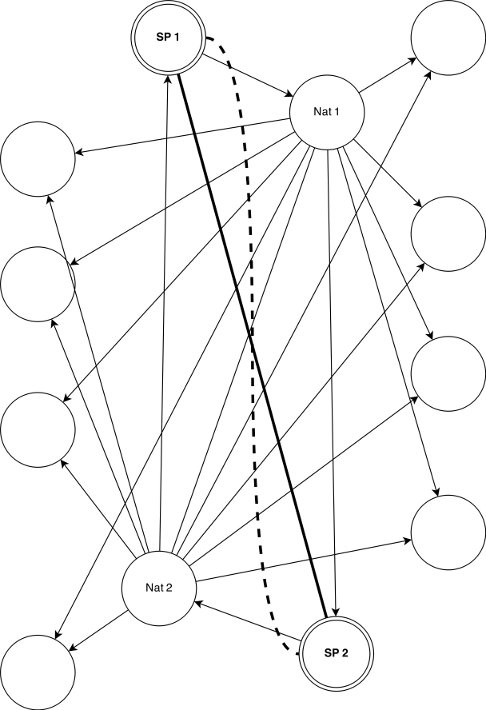
\includegraphics[scale=4.3]{Imagens/grafo.jpg}}
	\qquad
	\subfloat[Mapa de StarCraft] {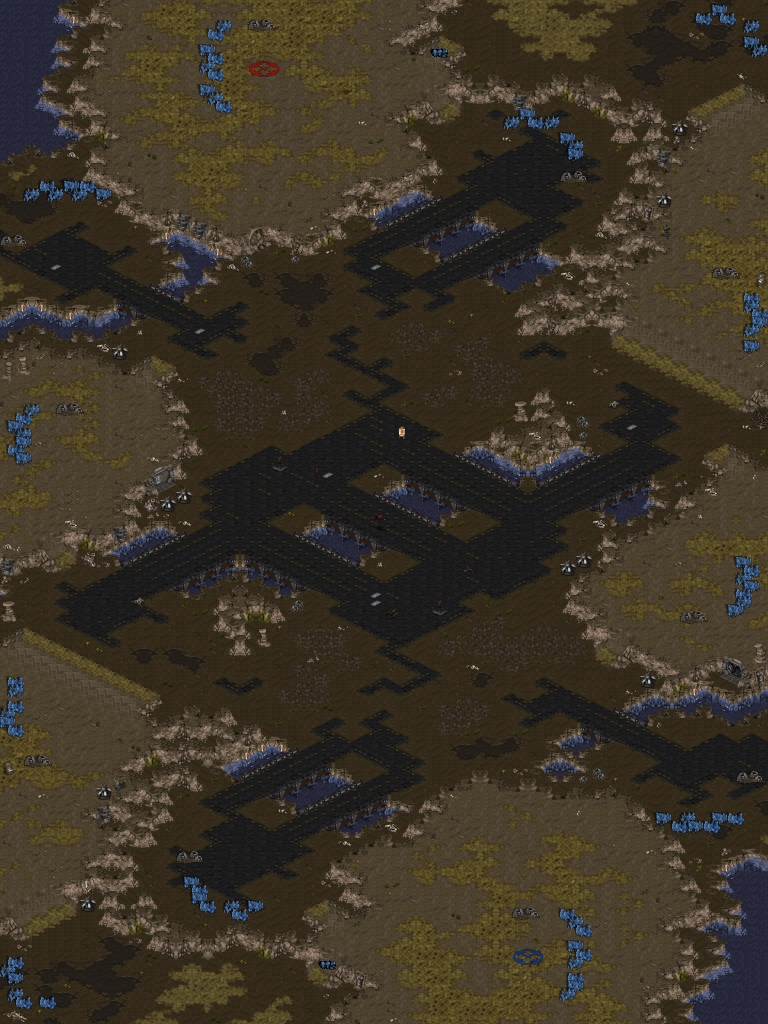
\includegraphics[scale=0.25]{Imagens/188_Destination.jpg}}
	\caption{Compara��o de mapa com o seu grafo correspondente}
	\label{fig:graph}
\end{figure}

A an�lise do mapa � feita de maneira est�tica criando um multigrafo direcionado de todas as bases principais, onde elas s�o ligadas por arestas que representam as dist�ncias terrestres e a�reas (Figura \ref{fig:graph}). Tamb�m ligadas �s bases est�o suas naturais, a partir delas pode-se chegar a todas as outras bases. A liga��o das outras bases �s naturais � feita somente pela dist�ncia terrestre.

\subsection{Verifica��o da movimenta��o e predi��o de ataques}
A verifica��o da movimenta��o se dar� atrav�s do uso de unidades terrestres de baixo custo e/ou de unidades a�reas que servir�o de unidades de reconhecimento. Elas ficar�o navegando pelo mapa � procura de pontos estrat�gicos para observar o ex�rcito inimigo, at� que haja perigo iminente, quando o ex�rcito do jogador precisar� se reagrupar.

Ap�s a primeira vista da movimenta��o, o agente far� uma aproxima��o da dire��o do movimento das unidades avistadas com alguns pontos de controle. Estes pontos de controle ser�o:
\begin{itemize}
	\item Expans�es, ocupadas ou n�o;
	\item Gargalos.
\end{itemize}

\citeonline{weber11} propuseram um modelo para estimar o movimento das unidades inimigas em StarCraft. Como esse modelo foi feito para receber treinamento vindo de \emph{replays} de partidas, uma proposta mais simples � utilizar algum conhecimento especialista para determinar os par�metros e eliminar o treinamento.

\subsection{Verifica��o do desenvolvimento estrat�gico do inimigo}
Al�m de unidades monitorando o ex�rcito inimigo, um grupo menor de unidades deve verificar as expans�es n�o ocupadas do mapa periodicamente, a fim de determinar quando uma expans�o foi tomada pelo inimigo. Espera-se que esse tipo de informa��o sirva para ativar algum tipo de resposta da intelig�ncia artificial, seja expandir ou atacar o inimigo.

Para verificar outros aspectos do desenvolvimento estrat�gico, o minist�rio deve verificar quais tecnologias foram pesquisadas e quais unidades foram criadas pelo inimigo, analisando os combates. Espera-se que essa informa��o seja usada para modelar um plano para combater o inimigo mais eficientemente.

\section{Comunica��o dos agentes}
Os agentes ir�o trocar informa��es em momentos diferentes do processo de atua��o da \emph{game AI}. Essas comunica��es podem ser categorizadas em comunica��es de depend�ncia e comunica��es de negocia��o.

As comunica��es de depend�ncia ocorrer�o quando, para realizar alguma a��o, um minist�rio precise de informa��es provenientes de outro. Esse tipo de comunica��o � a mais comum, j� que pode ocorrer a qualquer momento da execu��o da intelig�ncia artificial.

J� as comunica��es de negocia��o se dar�o quando a \emph{game AI} estiver no modo de rea��o e o minist�rio da ind�stria precisar atualizar a ordem de constru��o. Uma vez que cada agente ter� suas prefer�ncias quanto ao que se deve ser feito, a ind�stria recolher� o que cada um prefere e far� um leil�o a fim de decidir qual a melhor op��o para todos. Como entrada para esse leil�o, os agentes passar�o os resultados de fun��es de pertin�ncia referentes �s unidades que eles est�o respons�veis por observar.

\subsection{Comunica��es de Depend�ncia}
Comunica��es de depend�ncia ocorrem quando agentes precisam de informa��es ou a��es de outros agentes para atingir seu objetivo. Na Figura~\ref{fig:modelo}, os fluxos de comunica��o est�o demonstrados, do requisitador ao seu alvo. Abaixo, cada uma dessas requisi��es � explicada e categorizada de acordo com a a��o. Al�m destas, a negocia��o feita pelo Minist�rio da Ind�stria tamb�m � considerada uma comunica��o de depend�ncia, mas devido �s suas caracter�sticas, ela ser� explicada mais � frente.

\begin{itemize}
	\item Sele��o de aberturas
		\begin{itemize}
			\item Um or�culo insere a ordem de constru��o da abertura escolhida no Minist�rio da Ind�stria. Este or�culo � representado no gr�fico como Cerebrate, que � o conjunto de todos os minist�rios.
		\end{itemize}
\end{itemize}

\begin{itemize}
	\item Execu��o da ordem de constru��o
		\begin{enumerate}
			\item Antes de executar a ordem de constru��o, o Minist�rio da Ind�stria envia o or�amento da produ��o ao Minist�rio de Economia.
			\item Uma refer�ncia para o or�amento � repassada ao Minist�rio da Ind�stria, que a envia para o minist�rio respons�vel pela cria��o do item do topo da fila.
			\item Quando o item come�a a ser feito, o minist�rio respons�vel por ele manda o aviso que o or�amento foi cumprido para o Minist�rio de Economia.
		\end{enumerate}
\end{itemize}

\begin{itemize}
	\item Constru��o de estruturas
		\begin{enumerate}
			\item O Minist�rio da Ind�stria ordena ao Minist�rio de Infraestrutura a constru��o da estrutura que est� no topo da fila de produ��o.
			\item O Minist�rio de Infraestrutura procura o melhor posicionamento para tal estrutura, e pede ao Minist�rio de Minas o trabalhador livre mais pr�ximo da posi��o final escolhida.
			\item Ap�s o t�rmino da constru��o, o Minist�rio de Infraestrutura envia a estrutura para o minist�rio correspondente e o trabalhador usado de volta ao Minist�rio de Minas. Caso seja uma estrutura de produ��o, ela ir� para o Minist�rio da Ind�stria. Caso seja uma estrutura de pesquisa, o Minist�rio de Tecnologia se torna respons�vel por ela.
		\end{enumerate}
\end{itemize}

\begin{itemize}
	\item Cria��o de expans�es
		\begin{itemize}
			\item O Minist�rio de Infraestrutura, quando for construir uma expans�o, pede � Ag�ncia de Intelig�ncia qual a melhor posi��o para a pr�xima expans�o.
		\end{itemize}
\end{itemize}

\begin{itemize}
	\item Defesa de bases
		\begin{itemize}
			\item O Minist�rio da Defesa pede ao Minist�rio de Minas trabalhadores, quando n�o h� unidades suficientes para defender uma base.
		\end{itemize}
	\item Atualiza��o de informa��es importantes
		\begin{itemize}
			\item O Minist�rio da Defesa constantemente verifica com a Ag�ncia de Intelig�ncia quais s�o os pontos que precisam ser defendidos e quais precisam ser atacados.
			\item O Minist�rio da Tecnologia verifica com a Ag�ncia de Intelig�ncia quais tecnologias foram pesquisadas pelo oponente, para dar uma boa resposta � situa��o.
		\end{itemize}
	\item Destrui��o de estruturas
		\begin{enumerate}
			\item Quando uma estrutura � destru�da, o minist�rio respons�vel informa ao Minist�rio da Ind�stria.
			\item Ent�o, ele busca saber se existe a necessidade de reconstruir a estrutura atrav�s de uma negocia��o extraordin�ria.
		\end{enumerate}
\end{itemize}

\subsection{Comunica��es de Negocia��o}
\begin{table}[h]
	% T�tulo de tabelas sempre aparecem antes da tabela
	\center
	{
		\begin{tabular}{l|l}
			\hline
			\textbf{Agente}					&	\textbf{Unidades}\\
			\hline
			Minist�rio de Minas 			& 	Trabalhadores, bases\\
			Minist�rio da Ind�stria			&	Suprimentos\\
			Minist�rio da Economia 			&	Bases, estruturas de produ��o de unidades\\
			Minist�rio da Infraestrutura	&	Trabalhadores, Estruturas de defesa\\
			Minist�rio da Tecnologia		&	Estruturas de pesquisa, tecnologias\\
			Minist�rio de Defesa			&	Trabalhadores, unidades de combate,\\& estruturas de produ��o de unidades\\
			Ag�ncia de Intelig�ncia			&	Estruturas de defesa, unidades de combate, bases\\
			\hline
		\end{tabular}
	}
	\caption{Rela��o entre agentes e unidades}
	\label{tab:comneg}
\end{table}

Embora existam v�rios agentes que monitoram a necessidade de um mesmo tipo de unidade, eles observam sob diferentes perspectivas (tabela~\ref{tab:comneg}). Abaixo est�o descritas as motiva��es dos agentes com rela��o a cada tipo de unidade.

\begin{itemize}
	\item Trabalhadores:
		\begin{itemize}
		\item Minas: Procura obter a satura��o das bases.
		\item Defesa: Procura repor trabalhadores que morreram em combate.
		\end{itemize}
	\item Bases:
		\begin{itemize}
		\item Minas: Procura expandir quando h� mais trabalhadores que o necess�rio para opera��o das bases.
		\item Economia: Procura manter as estruturas de produ��o sempre funcionando.
		\item Intelig�ncia: Procura expandir depois de vencer uma batalha recente, pois o inimigo ter� que gastar tempo e recursos repondo tropas.
		\end{itemize}
	\item Suprimentos:
		\begin{itemize}
		\item Ind�stria: Procura n�o ficar com bloqueio de suprimentos.
		\end{itemize}
	\item Estruturas de produ��o:
		\begin{itemize}
		\item Economia: Procura aumentar o n�mero de estruturas, caso a renda d� suporte a isso, n�o importando que tipo de estrutura seja.
		\item Defesa: Procura criar estruturas que ajudem a construir um ex�rcito com uma determinada composi��o.
		\end{itemize}
	\item Estruturas de defesa:
		\begin{itemize}
		\item Infraestrutura: Procura deixar todas as bases com alta capacidade de defesa.
		\item Intelig�ncia: Procura aumentar o n�mero de estruturas de defesa ao perceber um ataque se aproximando.
		\end{itemize}
	\item Estruturas de pesquisa e tecnologias:
		\begin{itemize}
		\item Tecnologia: Procura construir estruturas que possam melhorar as unidades que est�o sendo produzidas.
		\end{itemize}
	\item Unidades de combate:
		\begin{itemize}
		\item Defesa: Procura fazer as melhores unidades, considerando o que � fact�vel e a composi��o desejada.
		\item Intelig�ncia: Procura fazer as melhores unidades, considerando o que � fact�vel e a composi��o inimiga.
		\end{itemize}
\end{itemize}
	
	% Capitulo 3: Terceiro captulo (arquivo Includes/Capitulo3.tex)
	% Cap�tulo 3
\chapter{Estudo de Caso em StarCraft}

O objetivo do estudo de caso deste trabalho � testar o modelo Cerebrate, proposto no cap�tulo anterior, no ambiente do jogo StarCraft. Devido ao problema de StarCraft ser bastante complexo, neste trabalho faremos testes em um contexto reduzido deste jogo com o intuito de comparar as aberturas no confronto Zerg versus Terran. Como o trabalho se focar� na ra�a Zerg, segue uma descri��o mais detalhada desta ra�a.

\section{A Ra�a Zerg}
A for�a dos \emph{Zerg} est� nos n�meros, e n�o em poucas unidades fortes. � a �nica ra�a que possui unidades que consomem menos que um suprimento: \emph{zerglings}\footnote{Primeira unidade de ataque \emph{zerg}. S� � capaz de atacar unidades terrestres, por ataques corpo-a-corpo.} e \emph{scourges}\footnote{Uma das primeiras unidades voadoras \emph{zerg}. S� � capaz de atacar unidades voadoras, por ataques corpo-a-corpo.} s�o produzidos aos pares e cada unidade consome meio suprimento. Suprimentos s�o aumentados com a produ��o de \emph{overlords} e bases. A base zerg fornece apenas um de suprimento, ao contr�rio dos 10 suprimentos do \emph{command center} dos Terran e dos 9 suprimentos do \emph{nexus} dos Protoss. A fonte padr�o de suprimentos, o overlord, al�m de aumentar a capacidade populacional tamb�m � a unidade \emph{detectora}\footnote{Unidade capaz de expor unidades invis�veis.} e o \emph{transporte}\footnote{Unidade voadora que pode carregar outras unidades dentro de si.}.

Suas estruturas de produ��o de unidades s�o tamb�m as estruturas de coleta de recurso. Elas produzem \emph{larvas}, de onde � poss�vel fazer qualquer unidade. Cada estrutura pode sustentar at� 3 larvas simultaneamente.

J� que n�o possuem estruturas dedicadas somente � produ��o de unidades, os Zerg possuem apenas estruturas que desbloqueiam unidades. Al�m disso, dependem da \emph{gosma} para constru��o dessas estruturas. Ela � espalhada ao redor de bases e de estruturas de defesa, \emph{creep colony}, \emph{spore colony} e \emph{sunken colony}.

Sua capacidade tecnol�gica depende do tipo de estrutura que serve de base, come�ando no primeiro n�vel tecnol�gico com a \emph{hatchery}, e seguindo com \emph{lair} e \emph{hive}, no segundo e terceiro n�veis, respectivamente. Isto significa que para desbloquear a possibilidade de constru��o de estruturas de segundo n�vel, � preciso evoluir a \emph{hatchery} para uma \emph{lair}.

\section{Simplifica��es do modelo}
Devido �s caracter�sticas da ra�a Zerg e � proposta do trabalho, que � de avaliar as aberturas que existem no confronto Zerg versus Terran, alguns aspectos do modelo Cerebrate foram alterados ou retirados.

Aberturas s�o ordens de constru��o que cont�m apenas estruturas e unidades. N�o h�, dentro do escopo delas, a possibilidade de alterar a ordem de constru��o ou de fazer alguma pesquisa tecnol�gica. Devido a essas caracter�sticas, constatamos que n�o h� a necessidade de controlar unidades militares ou de fazer pesquisas tecnol�gicas.

Portanto, as seguintes simplifica��es foram feitas:
\begin{itemize}
	\item A segunda fase do modelo, a rea��o, n�o ser� tratada. Como apenas as aberturas ser�o testadas, a parte do modelo que cuida do meio-jogo n�o � necess�ria.
	\item O Minist�rio de Tecnologia n�o ser� utilizado, pois as aberturas n�o requerem a pesquisa de nenhuma tecnologia.
	\item O Minist�rio de Defesa n�o ser� utilizado, pois as unidades militares n�o dever�o ser controladas.
	\item Como n�o haver� controle de unidades militares, a Ag�ncia de Intelig�ncia n�o se encarregar� de fazer tarefas de patrulhamento.
	\item O Minist�rio de Infraestrutura n�o liberar� trabalhadores, pois eles se tornam a pr�pria estrutura a ser constru�da, devido �s caracter�sticas espec�ficas da ra�a Zerg,.
\end{itemize}

As pr�ximas se��es descrevem detalhes da aplica��o do modelo Cerebrate em StarCraft.

\section{Estrutura do modelo}
Cada minist�rio do Cerebrate � estruturado hierarquicamente. Eles s�o representados como \emph{namespaces} que definem estruturas de controle e atua��o nas �reas espec�ficas de cada minist�rio. Em todos eles, h� uma estrutura que controla inst�ncias das outras estruturas que pertencem ao minist�rio. Esta estrutura controladora � o agente respons�vel pelo minist�rio. Estes agentes possuem as fun��es:

\begin{itemize}
 	\item \emph{update}: Atualiza as suas informa��es do controlador a cada quadro do jogo.
 	\item \emph{act}: Caso o agente possua unidades para controlar, esta fun��o � usada para dar ordens a essas unidades.
 \end{itemize}

A seguir est�o descritas as estruturas que comp�em os minist�rios.

\subsection{Minist�rio de Minas e do Trabalho}
\begin{figure}[h]
	\centering
	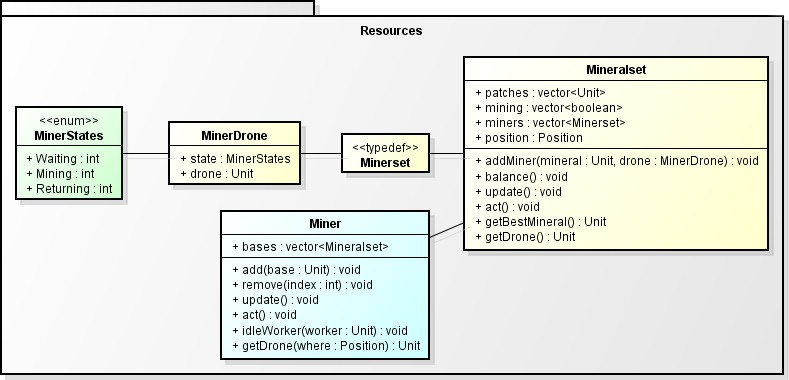
\includegraphics[scale=0.55]{Imagens/uml-mines.jpg}
	\caption{Diagrama de Classes das estruturas do Minist�rio de Minas e do Trabalho.}
	\label{fig:umlmines}
\end{figure}

A Figura~\ref{fig:umlmines} mostra o diagrama das estruturas que comp�em o minist�rio de minas. Ele possui uma estrutura para ligar trabalhadores a seus estados, a \emph{MinerDrone}. Esta estrutura � agrupada em um \emph{vector}, chamado \emph{Minerset}. Desta forma, existe uma estrutura que comporte todos os trabalhadores ligados a uma jazida de min�rios. Por�m, para a minera��o efetiva de uma base, s�o necess�rios outras informa��es e funcionalidades. A estrutura \emph{Mineralset} comporta as informa��es sobre as jazidas de min�rios (\emph{patches}), o estado destas jazidas (\emph{mining}), os trabalhadores ligados a elas (\emph{miners}) e a posi��o da base (\emph{position}). Al�m disso, possui as fun��es:
\begin{itemize}
	\item \emph{addMiner}: adiciona um novo trabalhador a uma das jazidas da base;
	\item \emph{balance}: equilibra a quantidade de trabalhadores por jazida de min�rio, para uma minera��o mais eficiente;
	\item \emph{getBestMineral}: retorna a jazida de min�rio mais pr�xima da posi��o da base e com menos trabalhadores por min�rio;
	\item \emph{getDrone}: retorna um trabalhador que n�o esteja minerando, caso exista.
\end{itemize}

A partir desta estrutura, podemos criar um conjunto de bases e faz�-las atuar como um conjunto. Para isso, foi feita a estrutura \emph{Miner}, que al�m de reunir as bases em um \emph{vector}, possui as funcionalidades:
\begin{itemize}
	\item \emph{add}: adiciona uma base rec�m criada;
	\item \emph{remove}: remove uma base, a partir do �ndice que esta base possui no \emph{vector} de bases;
	\item \emph{idleWorker}: esta fun��o � chamada ao identificar um trabalhador ocioso que ainda n�o fa�a parte do conjunto de mineradores do minist�rio;
	\item \emph{getDrone}: procura a base mais pr�xima do ponto dado e retorna o trabalhador dado pela fun��o \emph{getDrone} do \emph{Mineralset} que descreve esta base.
\end{itemize}

\subsection{Minist�rio da Economia}
\begin{figure}[h]
	\centering
	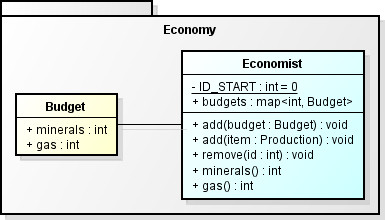
\includegraphics[scale=0.8]{Imagens/uml-economy.jpg}
	\caption{Diagrama de Classes das estruturas do Minist�rio da Economia.}
	\label{fig:umleco}
\end{figure}

O minist�rio da economia oferece um meio de gerenciar os itens cujo gasto n�o � imediato. Mostradas na Figura~\ref{fig:umleco}, as estruturas auxiliares s�o: \emph{Budget}, que descreve o valor dos itens, e \emph{Economist} que armazena os or�amentos atuais. Esta �ltima cont�m uma lista de or�amentos identificados por n�meros �nicos (\emph{budgets}) e prov� as seguintes fun��es:
\begin{itemize}
	\item \emph{add}: adiciona um or�amento ou um item � lista do minist�rio;
	\item \emph{remove}: remove o or�amento que possui a identifica��o dada;
	\item \emph{minerals}: retorna a quantidade de min�rios que o jogador pode gastar, isto �, os min�rios totais menos o valor em min�rios de todos os or�amentos;
	\item \emph{gas}: retorna a quantidade de g�s vespeno que o jogador pode gastar, utilizando-se da mesma l�gica.
\end{itemize}

\subsection{Ag�ncia de Intelig�ncia}
\begin{figure}[h]
	\centering
	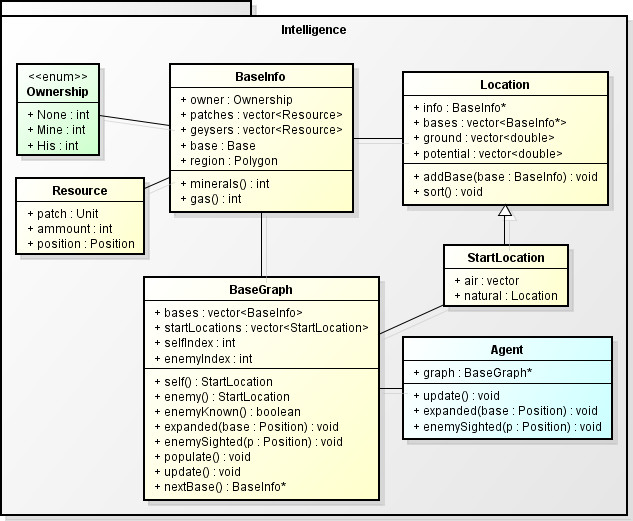
\includegraphics[scale=0.6]{Imagens/uml-intel.jpg}
	\caption{Diagrama de Classes das estruturas da Ag�ncia de Intelig�ncia.}
	\label{fig:umlintel}
\end{figure}

A ag�ncia de intelig�ncia ficou respons�vel por manter e atualizar o grafo de bases do mapa da partida. As estruturas e suas rela��es podem ser vistas na Figura~\ref{fig:umlintel}. Para descrever as bases, precisaremos de estruturas auxiliares que indiquem a posse da base (\emph{Ownership}) e o �ltimo estado conhecido dos recursos (\emph{Resource}). As bases (\emph{BaseInfo}) possuem estados de posse (\emph{owner}), jazidas de min�rios (\emph{patches}), g�iseres de g�s vespeno (\emph{geysers}), um pol�gono que descreve a regi�o and�vel (\emph{region}) e as informa��es dadas pela biblioteca de an�lise de terreno (\emph{base}). As fun��es \emph{minerals} e \emph{gas} retornam a quantidade total de recursos de uma base.

A partir destas informa��es sobre as bases, podemos criar um grafo. O grafo descreve as posi��es iniciais e as dist�ncias delas entre si, as naturais destas posi��es e as dist�ncias das naturais at� todas as outras bases. As naturais deste grafo s�o descritos pela estrutura \emph{Location}. Eles possuem a informa��o sobre a base (\emph{info}), os n�s adjacentes (\emph{bases}), a dist�ncia at� estes n�s (\emph{ground}) e o valor que cada n� adjacente possui (\emph{potential}). Para identificar a ordem de expans�o, esta estrutura possui a fun��o \emph{sort}, que ordena as bases pelo potencial e pela posse, deixando as bases com maior potencial e sem dono nas primeiras posi��es, e as bases com dono e menor potencial nas �ltimas posi��es.

Cada natural est� ligada a uma posi��o inicial, que � descrita pela estrutura \emph{StartLocation}. Al�m de conter informa��es sobre as dist�ncias terrestres entre as localiza��es iniciais do mapa, esta estrutura tamb�m possui as dist�ncias a�reas entre elas e a informa��o sobre a natural.

A estrutura \emph{BaseGraph} cont�m todas as informa��es necess�rias para o grafo. Ela guarda as informa��es de todas as bases do mapa (\emph{bases}), informa��es dos n�s do grafo (\emph{startLocations}) e a refer�ncia das posi��es iniciais do jogador e do inimigo (\emph{selfIndex} e \emph{enemyIndex}, respectivamente). Al�m disso, esta estrutura possui as fun��es:
\begin{itemize}
 	\item \emph{self}: retorna a posi��o inicial do jogador;
 	\item \emph{enemy}: retorna a posi��o inicial do inimigo;
 	\item \emph{enemyKnown}: retorna a posi��o inicial do inimigo � conhecida;
 	\item \emph{expanded}: altera a posse da base que fica na posi��o indicada, tornando-a do jogador;
 	\item \emph{enemySighted}: altera a posse da base que fica na posi��o indicada, tornando-a do inimigo;
 	\item \emph{populate}: chamada ap�s a an�lise de terreno, esta fun��o cria as informa��es da base e o grafo;
 	\item \emph{nextBase}: retorna a pr�xima base que o jogador deve tomar.
 \end{itemize}

 Como a ag�ncia de intelig�ncia ficou respons�vel apenas pelo grafo de bases, a estrutura \emph{Agent} serve como fachada para a \emph{BaseGraph}. Ele possui um ponteiro para ela, pois o grafo � alocado dinamicamente.

\subsection{Minist�rio da Infraestrutura}
\begin{figure}[h]
	\centering
	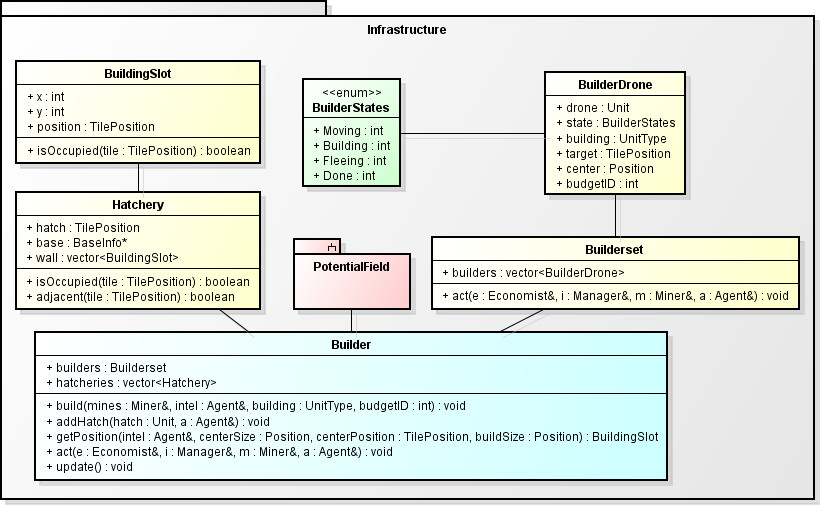
\includegraphics[scale=0.55]{Imagens/uml-infra.jpg}
	\caption{Diagrama de Classes das estruturas do Minist�rio de Infraestrutura.}
	\label{fig:umlinfra}
\end{figure}

O minist�rio de infraestrutura precisa de estruturas para controle de unidades, posicionamento pr�vio de estruturas e um conjunto de fun��es para o c�lculo de \emph{potential fields} (Figura~\ref{fig:umlinfra}). As estruturas de controle de construtores se assemelham �s estruturas do minist�rio de minas. \emph{BuilderStates} descreve quais estados comportamentais existem. \emph{BuilderDrone} faz a liga��o da unidade (\emph{drone}) com seu estado atual (\emph{state}), a constru��o que deve erguer (\emph{building}), a localiza��o da constru��o (\emph{target}), a posi��o que a unidade deve atingir para que possa construir (\emph{center}) e a identifica��o do or�amento no minist�rio da economia, para que se possa apagar o or�amento ap�s a constru��o.

O conjunto de construtores � organizado na estrutura \emph{Builderset}, que, al�m de possuir a lista destas unidades (\emph{builders}), possui a fun��o \emph{act}. Esta fun��o, como todas as outras com este nome, d� ordens �s unidades que est�o sob o controle da estrutura. Por�m, al�m disso, ela faz uso de outros minist�rios para atualiza��o de algumas informa��es:

\begin{itemize}
	\item \emph{Economist}: retira o or�amento que foi alocado para uma constru��o que tenha sido come�ada;
	\item \emph{Manager}: agente respons�vel pelo minist�rio da ind�stria, ele � chamado quando uma constru��o tenha sido cancelada;
	\item \emph{Miner}: quando uma nova base � conquistada, sua localiza��o � adicionada � lista de bases do minist�rio;
	\item \emph{Agent}: quando uma base � conquistada, seu estado de posse � alterado para ser do jogador.
\end{itemize}

Para alocar muralhas, foi necess�ria a cria��o de uma estrutura que descreva uma ``vaga'' para as constru��es. Esta estrutura, \emph{BuildingSlot}, possui o tamanho da constru��o em blocos de constru��o (\emph{x} e \emph{y}) e a posi��o da ``vaga'' (\emph{position}). Ela tamb�m oferece a fun��o \emph{isOccupied}, que retorna um booleano indicando se um determinado bloco de constru��o est� dentro da �rea de sua ``vaga''.

Como as muralhas s�o feitas a partir de uma base, elas foram descritas a partir disto. As bases est�o detalhadas na estrutura \emph{Hatchery}. Ela possui a posi��o da base (\emph{hatch}), as informa��es sobre ela (\emph{base}) e uma lista de aloca��es de estruturas para a muralha (\emph{wall}). Ela oferece as fun��es:

\begin{itemize}
	\item \emph{isOccupied}: informa se o bloco de constru��o est� dentro das �reas da muralha ou da base;
	\item \emph{adjacent}: informa se o bloco de constru��o � adjacente � base.
\end{itemize}

Finalmente, a estrutura que une todos estes conceitos � a \emph{Builder}. Ela possui as informa��es dos construtores (\emph{builders}) e das bases (\emph{hatcheries}). Suas fun��es s�o:

\begin{itemize}
	\item \emph{build}: solicita um trabalhador do minist�rio de minas (\emph{Miner}) e adiciona este trabalhador na lista de construtores;
	\item \emph{addHatch}: adiciona uma base � lista de bases da estrutura, al�m de alocar uma muralha para ela;
	\item \emph{getPosition}: retorna o alocamento de uma constru��o.
\end{itemize}

\subsection{Minist�rio da Ind�stria}
\begin{figure}[H]
	\centering
	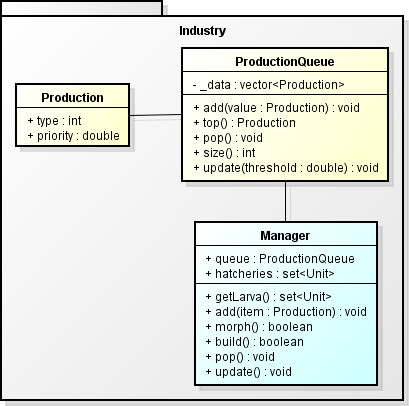
\includegraphics[scale=0.55]{Imagens/uml-industry.jpg}
	\caption{Diagrama de Classes das estruturas do Minist�rio da Ind�stria.}
	\label{fig:umlindustry}
\end{figure}

O minist�rio da ind�stria possui uma fila de prioridades (\emph{ProductionQueue}) para os itens da ordem de constru��o (\emph{Production}). Cada item pode ser ou uma unidade (\emph{type}), o que inclui constru��es tamb�m, ou uma pesquisa (\emph{tech}), al�m de possuir um valor que indica a sua prioridade (\emph{priority}). As filas atualizam todo quadro para retirar os elementos que possuem um valor de prioridade menor que um determinado limiar (\emph{threshold}).

A estrutura controladora da fila, a \emph{Manager}, possui tanta a fila (\emph{queue}) como as estruturas de produ��o (\emph{hatcheries}). Para facilitar o acesso das larvas que existem em todas as \emph{hatcheries}, a fun��o \emph{getLarva} junta todas as larvas em um �nico conjunto. Para cria��o das aberturas, a fun��o \emph{add} foi criada, recebendo o item a ser inserido. As outras fun��es existem para auxiliar a fun��o \emph{update}:

\begin{itemize}
	\item \emph{morph}: caso o primeiro item seja uma unidade, esta fun��o seleciona uma larva e cria a unidade;
	\item \emph{build}: caso o item seja uma constru��o, esta fun��o chama a fun��o \emph{build} da \emph{Miner};
	\item \emph{pop}: esta fun��o que avalia os itens e chama as fun��es necess�rias para o cumprimento da a��o;
\end{itemize}

\subsection{Cerebrate}
\begin{figure}[H]
	\centering
	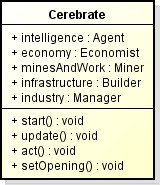
\includegraphics[scale=0.8]{Imagens/uml-cerebrate.jpg}
	\caption{Estrutura do Cerebrate.}
	\label{fig:umlindustry}
\end{figure}

O Cerebrate cont�m uma inst�ncia de cada agente dos minist�rios. Eles s�o atualizados na ordem: (a) Ag�ncia de Intelig�ncia, (b) Minist�rio de Infraestrutura, (c) Minist�rio de Minas e do Trabalho e (d) Minist�rio da Ind�stria. Al�m das fun��es comuns a todos os agentes, o Cerebrate tamb�m possui:

\begin{itemize}
	\item \emph{start}: o jogo come�a no quadro 0, e neste quadro esta fun��o especial de inicializa��o, respons�vel pela an�lise de terreno e a configura��o inicial de todos os agentes, � chamada;
	\item \emph{setOpening}: durante esta fase inicial, a escolha da abertura a ser utilizada � feita atrav�s desta fun��o.
\end{itemize}

\section{Escolha de aberturas}
Para decidir qual abertura tomar, a \emph{game AI} verificar� as dist�ncias terrestres entre as principais. Caso haja mais de duas posi��es iniciais e n�o se saiba a posi��o do oponente a tempo de fazer uma escolha, ele assume que cada valor ser� a m�dia das dist�ncias correspondentes entre todas as principais e naturais. Essas dist�ncias ser�o, ent�o, passadas para fun��es de pertin�ncia referentes �s aberturas escolhidas para esse trabalho. As dist�ncias s�o dadas em uma unidade de dist�ncia $D$, que � a dist�ncia correspondente � largura de um pixel no mapa, e passadas para as fun��es em unidades de $kD$, $10^3 D$. As fun��es de pertin�ncia para as dist�ncias, cujo gr�fico est� mostrado na Figura~\ref{fig:graphdist}, s�o as seguintes:
%\begin{equation}
%	\displaystyle
%	tanh(x) = \frac{1-e^{-2x}}{1+e^{-2x}}
%\end{equation}
\begin{equation}
	\displaystyle
	\text{5 pool}_d = \Big(1 -\dfrac{tanh(2(terrestre-5))+1}{2}\Big)^2
\end{equation}
\begin{equation}
	\displaystyle
	\text{9 pool}_d = \mathlarger{\mathlarger{e}}^{-\dfrac{(terrestre-4.5)^2}{0.32}}
\end{equation}
\begin{equation}
	\displaystyle
	\text{Overpool}_d = \mathlarger{\mathlarger{e}}^{-\dfrac{(terrestre-5)^2}{0.8}}
\end{equation}
\begin{equation}
	\displaystyle
	\text{12 pool}_d = \mathlarger{\mathlarger{e}}^{-\dfrac{(terrestre-5.5)^2}{0.64}}
\end{equation}
\begin{equation}
	\displaystyle
	\text{12 hatch}_d = \dfrac{tanh(1.5(terrestre-5))+1}{2}
\end{equation}

\begin{figure}[h]
	\centering
	\begin{tikzpicture}
		\begin{axis}[
			width=15cm,height=6.4cm,
			xtick={3,4,...,7},
			xlabel={\footnotesize{Dist�ncia Terrestre entre as Principais em $kD$}},
			xmin=3,
			xmax=7,
			legend style={at={(0,0.25)},anchor=south west}]

			\addplot[domain=3:7, color={sixpool}, samples=200] {(1-(tanh(2*x-10)+1)/2)^2};
			\addlegendentry{5 pool}

			\addplot[domain=3:7, color={ninepool}, samples= 200] {e^((x-4.5)^2/-0.32)};
			\addlegendentry{9 pool}
			\addplot[domain=3:7, color={overpool}, samples=200] {e^((x-5)^2/-0.8)};
			\addlegendentry{Overpool}
			\addplot[domain=3:7, color={twelpool}, samples=200] {e^((x-5.5)^2/-0.64)};
			\addlegendentry{12 pool}
			\addplot[domain=3:7, color={twelhatch}, samples=200] {(tanh(1.5*x-7.5)+1)/2};
			\addlegendentry{12 hatch}
		\end{axis}
	\end{tikzpicture}
	\caption{Gr�fico das fun��es de pertin�ncia das dist�ncias}
	\label{fig:graphdist}
\end{figure}

Logo ap�s, s�o calculadas as pertin�ncias referentes � passividade do Cerebrate. As fun��es foram modeladas de forma que quanto maior a passividade, menor a pertin�ncia nas aberturas agressivas (\emph{rushes} e \emph{cheeses}) e maior a pertin�ncia nas aberturas mais tradicionais. O gr�fico dessas fun��es est� plotado na Figura~\ref{fig:graphpas}.

\begin{equation}
	\displaystyle
	\text{5 pool}_p = \left(1 - \dfrac{tanh(5(passividade-0.5))+1}{2}\right)^2
\end{equation}
\begin{equation}
	\displaystyle
	\text{9 pool}_p = \mathlarger{\mathlarger{e}}^{-\dfrac{(passividade-0.2)^2}{0.08}}
\end{equation}
\begin{equation}
	\displaystyle
	\text{Overpool}_p = \mathlarger{\mathlarger{e}}^{-\dfrac{(passividade-0.3)^2}{0.12}}
\end{equation}
\begin{equation}
	\displaystyle
	\text{12 pool}_p = \mathlarger{\mathlarger{e}}^{-\dfrac{(passividade-0.43)^2}{0.06}}
\end{equation}
\begin{equation}
	\displaystyle
	\text{12 hatch}_p = \dfrac{tanh(2(passividade-0.1))+1}{2}
\end{equation}

\begin{figure}[h]
	\centering
	\begin{tikzpicture}
		\begin{axis}[
			width=15cm,height=6.4cm,
			xlabel={\footnotesize{Passividade}},
			legend style={at={(1,0.25)},anchor=south east},
			xmin=0,
			xmax=1]

			\addplot[domain=0:1, color={sixpool}, samples=200] {(1-((tanh(5*x-2.5)+1)/2))^2};
			\addplot[domain=0:1, color={ninepool}, samples=200] {e^(-(x-0.2)^2/0.08)};
			\addplot[domain=0:1, color={overpool}, samples=200] {e^(-(x-0.3)^2/0.12)};
			\addplot[domain=0:1, color={twelpool}, samples=200] {e^(-(x-0.5)^2/0.06)};
			\addplot[domain=0:1, color={twelhatch}, samples=200] {(tanh(2*(x-0.1))+1)/2};
			\legend{5 pool, 9 pool, Overpool, 12 pool, 12 hatch}
		\end{axis}
	\end{tikzpicture}
	\caption{Gr�fico das fun��es de pertin�ncia da passividade}
	\label{fig:graphpas}
\end{figure}

A partir das pertin�ncias de dist�ncia e passividade, � poss�vel calcular o valor da pertin�ncia final das aberturas, que se dar� ao utilizar o operador fuzzy \emph{ou}\footnote{O operador fuzzy \emph{ou} utilizado tem como significado uma opera��o de uni�o: $\mu_{a \cup b} = \mu(a) + \mu(b) - \mu(a)\mu(b)$.} sobre os dois valores. Isto �:

\begin{equation}
	\displaystyle
	\text{5 pool} = \text{5 pool}_d \lor \text{5 pool}_p
\end{equation}
\begin{equation}
	\displaystyle
	\text{9 pool} = \text{9 pool}_d \lor \text{9 pool}_p
\end{equation}
\begin{equation}
	\displaystyle
	\text{Overpool} = \text{Overpool}_d \lor \text{Overpool}_p
\end{equation}
\begin{equation}
	\displaystyle
	\text{12 pool} = \text{12 pool}_d \lor \text{12 pool}_p
\end{equation}
\begin{equation}
	\displaystyle
	\text{12 hatch} = \text{12 hatch}_d \lor \text{12 hatch}_p
\end{equation}

Ap�s o c�lculo final, a escolha � feita aleatoriamente entre as duas aberturas com maiores pertin�ncias. Cada uma delas possui chance proporcional � sua pertin�ncia em rela��o � soma das duas maiores, ou seja:
\begin{equation}
	\displaystyle
	chance_a = \dfrac{pertinencia_a}{pertinencia_a+pertinencia_b}
\end{equation}
\begin{equation}
	\displaystyle
	chance_b = \dfrac{pertinencia_b}{pertinencia_a+pertinencia_b}
\end{equation}

\section{Expans�o econ�mica}
Para a cria��o do grafo de bases, primeiro s�o achadas as bases correspondentes �s posi��es iniciais do mapa, isto �, todas as principais do mapa. Ent�o, procura-se a base mais pr�xima a cada uma das posi��es iniciais. Estas bases s�o as naturais e s�o atribu�das a suas respectivas principais. Ap�s isso, o grafo � completado com as dist�ncias terrestres das naturais para todas as outras bases, que n�o s�o suas principais. As bases atribu�das � natural do jogador s�o ordenadas de acordo com uma fun��o que avalia o potencial de minera��o de uma base e de acordo com o dono dessa base. Bases que possuem dono s�o as �ltimas, enquanto bases livres e com alto potencial s�o as primeiras da lista de bases.

A fun��o de potencial das bases � calculada baseada nas seguintes propriedades:
\begin{itemize}
	\item Quantidade de jazidas de min�rio
	\item Quantidade total de min�rios dispon�veis\footnote{Como a priori n�o sabe-se quantos min�rios existem em cada jazida, utiliza-se o valor padr�o de $1500$.}
	\item Quantidade total de g�s vespeno dispon�vel\footnote{Da mesma forma que os min�rios, utiliza-se o valor padr�o de $5000$ para expressar o valor desconhecido.}
	\item Dist�ncia at� a base principal
	\item Dist�ncia at� a base do oponente
\end{itemize}

Cada uma dessas propriedades � passada para uma fun��o de pertin�ncia espec�fica para ela, e ent�o passadas para uma fun��o que calcula o potencial da expans�o. As dist�ncias s�o passadas para a fun��o $dist$ em $kD$, a quantidade de min�rios nas jazidas e a quantidade de vespeno nos g�iseres s�o passadas em unidades de $10^3$. O gr�fico da fun��o $dist$ e das outras fun��es de pertin�ncias podem ser vistos na Figura~\ref{fig:graphs}.

A fun��o $dist$ retorna um valor fuzzy referente a qu�o distante um ponto est� do outro. Ela foi modelada de acordo com os mapas usados nas competi��es existentes de \emph{game AI} para StarCraft. As dist�ncias entre as principais de cada mapa foram verificadas e uma fun��o sigm�ide foi modelada baseando-se nas dist�ncias mais curtas e mais longas encontradas nos mapas. Esta fun��o � usada nas fun��es referentes � dist�ncia para a base do jogador e � dist�ncia para a base do oponente.

A fun��o que avalia a proximidade de bases para a principal do jogador retorna o valor 0 caso a base avaliada seja uma ilha. Caso contr�rio, retorna a nega��o\footnote{A nega��o fuzzy se d� pela fun��o: $\neg(x) = 1 - x$.} da fun��o $dist$ aplicada � dist�ncia entre as duas bases. Desta forma, a fun��o tende a retornar 1 � medida em que a dist�ncia entre as bases tende a 0.

A fun��o que avalia a proximidade de bases para a principal do oponente segue uma l�gica similar, por�m com valores opostos. Caso o oponente n�o seja conhecido, as dist�ncias entre as bases n�o podem ser verificadas, ent�o o retorno � 1. Isto �, n�o h� efeitos negativos no potencial da base avaliada. Caso a base avaliada esteja em uma ilha, o retorno tamb�m � 1. Caso a base seja a natural ou a principal do opoenente, o retorno � 0, pois elas s�o as bases mais pr�ximas da base principal do oponente. No caso padr�o, a fun��o retorna o valor de $dist$ aplicada � dist�ncia entre a base avaliada e a principal do oponente. Desta forma, quanto menor a dist�ncia da base avaliada para a base inimiga, menor o potencial dela.

A fun��o de pertin�ncia relativa � quantidade de jazidas foi modelada de acordo com o que foi encontrado nos mapas das competi��es. Na maioria dos mapas, as bases principais possuem 9 jazidas de min�rios, suas naturais possuem 8 e as outras bases possuem 7 jazidas. J� que, quanto maior o n�mero de jazidas, mais trabalhadores podem trabalhar paralelamente para recoltamento de min�rios, a fun��o descreve uma sigm�ide cujo valor tende a 1 conforme o n�mero de jazidas aumenta.

A quantidade de min�rios � avaliada de maneira similar, tendo em vista que a maior parte das bases principais possuem 13.500 min�rios espalhados em 9 jazidas, cada uma com 1.500 min�rios. Ela tamb�m descreve uma sigm�ide que tende a 1 � medida que a quantidade de min�rios numa base aumenta.

A quantidade de g�s vespeno numa base � avaliada linearmente com um m�nimo de 0,5, pois a sua influ�ncia na escolha de bases � baixa. Isto se deve pelo fato da coleta de g�s vespeno ser muito alta em rela��o � coleta de min�rios e � taxa com a qual o g�s � usado durante uma partida.

As fun��es de pertin�ncia s�o:

\begin{figure}[h]
	\centering
	\subfloat[Gr�fico da fun��o $dist$] {
		\begin{tikzpicture}
			\begin{axis}[
				width=7cm,height=5cm,
				xtick={0,1,...,4},
				xlabel={\footnotesize{Dist�ncia Terrestre entre bases ($10^3$)}},
				xmin=0,
				xmax=4,
				legend style={at={(0,0.75)},anchor=south west}]

				\addplot[samples=200, color={distance}] {((tanh(1.5*x-3)+1)/2)};
				\addlegendentry{dist}
			\end{axis}
		\end{tikzpicture}
	}
	\qquad
	\subfloat[Gr�fico da fun��o de pertin�ncia das jazidas] {
		\begin{tikzpicture}
			\begin{axis}[
				width=7cm,height=5cm,
				xtick={4,5,...,9},
				xlabel={\footnotesize{Quantidade de jazidas de min�rios}},
				xmin=4,
				xmax=9,
				legend style={at={(0,0.75)},anchor=south west}]

				\addplot[samples=200, color={patches}][domain=0:10] {( ( tanh( 0.5*x - 2.5) + 1 )/2 )^3};
				\addlegendentry{jazidas}
			\end{axis}
		\end{tikzpicture}
	}
	\qquad
	\subfloat[Gr�fico da fun��o de pertin�ncia dos min�rios] {
		\begin{tikzpicture}
			\begin{axis}[
				width=7cm,height=5cm,
				xtick={1,2,...,12},
				xlabel={\footnotesize{Quantidade de min�rios nas jazidas ($10^3$)}},
				xmin=0,
				xmax=12,
				legend style={at={(0,0.75)},anchor=south west}]

				\addplot[samples=200, color={minerals}][domain=0:15] {( tanh( 0.3*x - 1.8) + 1 )/2};
				\addlegendentry{minerios}
			\end{axis}
		\end{tikzpicture}
	}
	\qquad
	\subfloat[Gr�fico da fun��o de pertin�ncia do g�s] {
		\begin{tikzpicture}
			\begin{axis}[
				width=7cm,height=5cm,
				xtick={0,1,...,6},
				ytick={0,0.5,1},
				ymin=-0.1,
				xlabel={\footnotesize{Quantidade de g�s nos g�iseres ($10^3$)}},
				xmin=0,
				xmax=6,
				legend style={at={(0,0.75)},anchor=south west}]

				\addplot[samples=200, color={gas}][domain=0:7] {min(x/10 + 0.5,1)};
				\addlegendentry{gas}
			\end{axis}
		\end{tikzpicture}
	}
	\caption{Gr�ficos das fun��es de pertin�ncia que auxiliam a classifica��o das bases.}
	\label{fig:graphs}
\end{figure}

\begin{equation*}
	\displaystyle
	dist(x) = \frac{tanh(1.5x - 3) + 1}{2}
\end{equation*}

\begin{equation*}
	\displaystyle
	dist_{principal}(b) = \left\{
		\begin{array}{l l}
		0 & , \text{b.ilha(})\\
		1 - dist(\text{jogador.natural.distancia(b)}) & , \text{ caso contr�rio}
		\end{array}\right.
\end{equation*}

\begin{equation*}
	\displaystyle
	dist_{oponente}(b) = \left\{
		\begin{array}{l l}
		1 & ,
		\begin{array}{l}
		\text{b.ilha()} \lor\\
			\neg \text{ oponente.conhecido()}
		\end{array}\\
		0 & , 
		\begin{array}{l}
		b = \text{oponente.principal()} \lor\\
		b = \text{oponente.natural()}
		\end{array}\\
		dist(\text{oponente.natural.distancia(b)}) & , \text{ caso contr�rio}		
		\end{array}\right.
\end{equation*}

\begin{equation*}
	\displaystyle
	\text{jazidas}(b) = \left(\frac{tanh\left(\frac{\text{b.jazidas()}-5}{2}\right) + 1}{2}\right)^3
\end{equation*}

\begin{equation*}
	\displaystyle
	\text{minerios}(b) = \frac{tanh\left(0.3\left(\text{b.minerios()} - 6\right)\right) + 1}{2}
\end{equation*}

\begin{equation*}
	\displaystyle
	\text{gas}(b) = min\left\{\frac{b.gas()}{10} + 0.5, 1\right\}
\end{equation*}

\begin{equation*}
	\displaystyle
	\text{potencial}(b) = (dist_{principal}(b) \times dist_{inimigo}(b))(minerios(b) \times jazidas(b) \times gas(b))
\end{equation*}

Como podem haver mapas com mais de duas posi��es iniciais, utiliza-se a m�dia das dist�ncias entre a base em quest�o e as posi��es iniciais em que o inimigo pode estar.

\section{Minist�rio de Minas e Trabalho}
O Minist�rio de Minas e Trabalho foi organizado de forma que ele seja uma cole��o de agentes, relacionados a cada trabalhador. Cada agente est� agrupado de acordo com a jazida que est� coletando. Estas jazidas, por sua vez, est�o agrupadas de acordo com a base que est� mais pr�xima a elas.

Dessa forma, existem duas formas de otimizar a minera��o. Uma no que diz respeito � quantidade de trabalhadores em cada jazida de uma base, e a outra na quantidade de trabalhadores por base que o jogador possui.

No caso de teste, nos focaremos na otimiza��o de trabalhadores por min�rios, j� que n�o passaremos da fase de abertura do jogo.

\section{Minist�rio de Infraestrutura}
O Minist�rio de Infraestrutura tem como um de seus objetivos escolher a posi��o onde as estruturas ser�o constru�das. Para calcular o posicionamento, escolhemos o m�todo \emph{potential fields} que atribui cargas a alguns elementos do jogo, como obst�culos ou unidades, e calcula o valor potencial dos blocos a partir da influ�ncia destes elementos no bloco analisado.

Inicialmente, � necess�rio definir quais elementos receber�o carga. Aqui, usaremos cargas positivas como atrativas e cargas negativas como repulsivas. Como visto no cap�tulo anterior, os pontos no per�metro da regi�o devem receber carga atrativa, pois o objetivo � criar uma muralha de estruturas em uma determinada base. Esse per�metro � calculado segundo a t�cnica de \citeonline{perkins10}. A influ�ncia do per�metro sobre um bloco de constru��o � determinada pela dist�ncia do per�metro ao bloco. Como o per�metro � dado em segmentos de reta, essa dist�ncia � calculada de acordo com a proje��o do ponto correspondente ao bloco em cada um dos segmentos de reta (Figura~\ref{fig:dist}) e escolhendo menor dist�ncia entre o ponto projetado e o ponto correspondente ao bloco. Ap�s esse c�lculo, o valor da influ�ncia do per�metro � determinado por uma fun��o de potencial. A fun��o de potencial usada por este trabalho �:

\begin{equation}
	\displaystyle
	potencial(q,p_c,p_b)=\frac{q}{dist(p_c,p_b)^2}
	\label{eq:perim}
\end{equation}

Onde $q$ � a carga do objeto, $p_c$ � a posi��o do objeto carregado no mapa e $p_b$, a posi��o do bloco em quest�o. A carga dos pontos do per�metro � igual a $400$. Como um bloco de constru��o ocupa um quadrado de $32 \times 32$ pixels, utiliza-se a m�dia dos valores correspondentes a cada um dos quatro cantos que esse bloco ocupa no mapa. Essa t�cnica de utilizar a m�dia das influ�ncias sobre os quatro pontos ser� usada por todos os outros elementos com carga.

Outros elementos que receber�o carga s�o os recursos. Para n�o colocar constru��es que bloqueiem sua coleta, eles recebem carga repulsiva. Como cada recurso possui �reas diferentes, sua carga ser� proporcional � sua �rea. Ao contr�rio do per�metro, cada recurso possui apenas um ponto fixo no mapa, de forma que para calcular a influ�ncia, basta verificar a dist�ncia at� o recurso. Cada recurso da regi�o � levado em considera��o, ao contr�rio do mais pr�ximo. A carga das jazidas de min�rios � igual a $-13000$, e a carga dos g�iseres de g�s vespeno � igual a $-52000$.

Al�m desses, os gargalos tamb�m receber�o carga repulsiva. Gargalos possuem uma posi��o e uma largura, dada em pixels. A influ�ncia deles ir� depender desses dois fatores, de forma que a carga para os gargalos � igual a $-1000l$, onde $l$ � a largura do gargalo.

Al�m de levar em conta esses fatores, o valor do bloco de constru��o � limitado pelo intervalo $[-80,80]$ inicialmente e pode receber penalidades que o fa�am superar esse intervalo:
\begin{itemize}
 	\item $-160$, caso o modo de busca por posicionamento seja tradicional, ao inv�s de cria��o de muralhas, e o bloco esteja fora da gosma;
 	\item $-80$, caso o bloco n�o seja constru�vel ou esteja dentro de alguma aloca��o feita anteriormente;
 \end{itemize}

Sabe-se que toda muralha zerg necessita de duas \emph{hatcheries}, uma servindo como base e outra servindo como \emph{macro hatch}\footnote{\emph{Hatchery} criada apenas para produ��o de unidades, ao inv�s de servir como dep�sito de recursos.}, como mostrado na Figura~\ref{fig:zwall}. Tendo em vista isso, e que a maior parte das \emph{macro hatches} ficam na regi�o mais distante, o que se prop�e � iniciar a aloca��o da muralha com o posicionamento de uma \emph{hatchery} utilizando todas essas cargas e fun��es. Em seguida, utilizar uma carga atrativa para base ao inv�s do per�metro, cujo valor � igual a $20000$. Utiliza-se o ponto central da estrutura como refer�ncia. Al�m disso, todas as outras cargas tamb�m s�o utilizadas e somadas �s devidas penalidades por construtibilidade, para que o algoritmo complete a muralha.

\begin{figure}
	\centering
	\subfloat{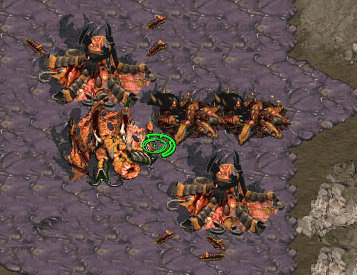
\includegraphics[scale=0.4]{Imagens/zwall3.jpg}}
	\qquad
	\subfloat{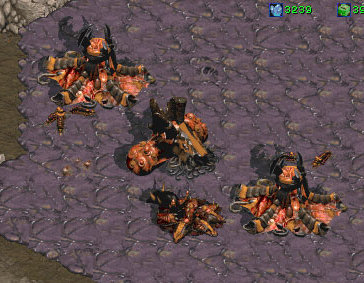
\includegraphics[scale=0.4]{Imagens/zwall2.jpg}}
	\qquad
	\subfloat{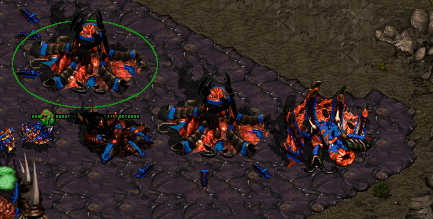
\includegraphics[scale=0.4]{Imagens/zwall1.png}}
	\caption[Muralhas Zerg em v�rios mapas.]{Muralhas Zerg em v�rios mapas. Aqui � poss�vel observar a exist�ncia de duas \emph{hatcheries} em todas as muralhas. H� tamb�m uma tend�ncia de utilizar estruturas de defesa para preencher as brechas existentes na muralha.}
	\label{fig:zwall}
\end{figure}

Para calcular o valor do posicionamento de uma estrutura, ser� utilizada a soma dos valores de influ�ncia de cada um dos blocos dentro da �rea da estrutura. A partir disso, deve-se seguir o seguinte algoritmo para a aloca��o de muralhas:

\begin{enumerate}
	\item Alocar uma \emph{hatchery}, ou estrutura $4\times3$, no melhor posicionamento dentro da regi�o da base escolhida, utilizando as fun��es mencionadas acima.
	\item At� que a base esteja adjacente a alguma estrutura alocada na muralha, repita:
	\begin{enumerate}
		\item Para cada �rea que estruturas podem ocupar (para Zergs, isto significa, efetivamente, $\{2\times2, 3\times2\}$):
		\begin{enumerate}
			\item Achar o melhor posicionamento poss�vel para a �rea que seja adjacente � �ltima estrutura alocada, usando apenas a base como elemento carregado.
		\end{enumerate}
		\item Selecionar o melhor valor de todas as �reas e alocar na muralha.
	\end{enumerate}
\end{enumerate}

Deixando a aloca��o de estruturas mais gen�rica, o sistema de tomada de decis�es poder� tentar otimizar as brechas, o custo ou o tempo de constru��o da muralha, tendo em vista as �reas alocadas.

Atrav�s dos direcionamentos tomados, conseguimos aplicar o modelo Cerebrate no jogo StarCraft, utilizando a ra�a Zerg como foco do trabalho. No pr�ximo cap�tulo, apresentaremos experimentos pr�ticos para valida��o do modelo.
	
	% Capitulo 4: Quarto captulo (arquivo Includes/Capitulo4.tex)
	% Cap�tulo 4
\chapter{Experimentos}

\section{Metodologia}
Cerebrate foi implementado em C++, utilizando o Visual C++ 2008 Express. O c�digo-fonte da implementa��o deste modelo est� armazenado no site: \url{https://github.com/caiofreitaso/Cerebrate}.

Para implement�-lo, foi utilizada a BWAPI 3.7.6\footnote{\url{http://bwapi.github.io}}. Esta API � o \emph{framework} usado para interagir com StarCraft. Ela prov� v�rias funcionalidades que permitem estudantes e pesquisadores criar \emph{game AIs} para esse jogo. Al�m das funcionalidades, a API exp�e ao programador todas as informa��es necess�rias para o controle e verifica��o do estado atual do jogo. Os m�dulos criados com esta API devem ser injetados dentro do processo do jogo atrav�s de um programa chamado Chaoslauncher\footnote{http://wiki.teamliquid.net/starcraft/Chaoslauncher}, utilizando um \emph{plug-in} espec�fico para a BWAPI. Dessa forma, o Chaoslauncher d� acesso �s informa��es do jogo para o m�dulo criado.

Os minist�rios do Cerebrate necessitam de dados de an�lise de terreno como a localiza��o das bases e as regi�es constru�veis. Estes dados s�o adquiridos com o uso da BWTA 1.7.1\footnote{\url{https://code.google.com/p/bwta/}}. A BWTA � uma biblioteca de an�lise de terreno para a BWAPI. Ela implementa uma t�cnica de identifica��o de regi�es no mapa e as separa atrav�s de gargalos. Esta t�cnica � descrita por \citeonline{perkins10}, e a biblioteca foi criada pelo mesmo autor. Al�m dessa t�cnica, a biblioteca implementa uma busca pelas localiza��es das bases no mapa que est� sendo jogado. Estas localiza��es s�o usadas pela Ag�ncia de Intelig�ncia para decidir a ordem de expans�es.

Os experimentos foram realizados nos mapas Destination\footnote{\url{http://wiki.teamliquid.net/starcraft/Destination}} e Fighting Spirit\footnote{\url{http://wiki.teamliquid.net/starcraft/Fighting_Spirit}} (Figura~\ref{fig:maps}). Estes foram os mapas mais jogados em competi��es, com 1196 e 1052 partidas em competi��es oficiais, respectivamente. Eles tamb�m s�o amplamente utilizados em ligas de jogadores amadores como na liga iCCup\footnote{\url{http://iccup.com/en/starcraft/}}. Por serem mapas competitivos, o seu objetivo original � a destrui��o de todas as estruturas inimigas. Por�m, este objetivo n�o ser� utilizado devido ao foco da pesquisa.

Apenas um experimento foi realizado para cada caso de teste. Como o posicionamento das unidades e dos recursos � est�tica, e a ordem dada �s unidades � determin�stica, v�rios experimentos feitos nas mesmas condi��es apresentaram os mesmos resultados.

\begin{figure}[H]
	\centering
	\subfloat[Fighting Spirit] {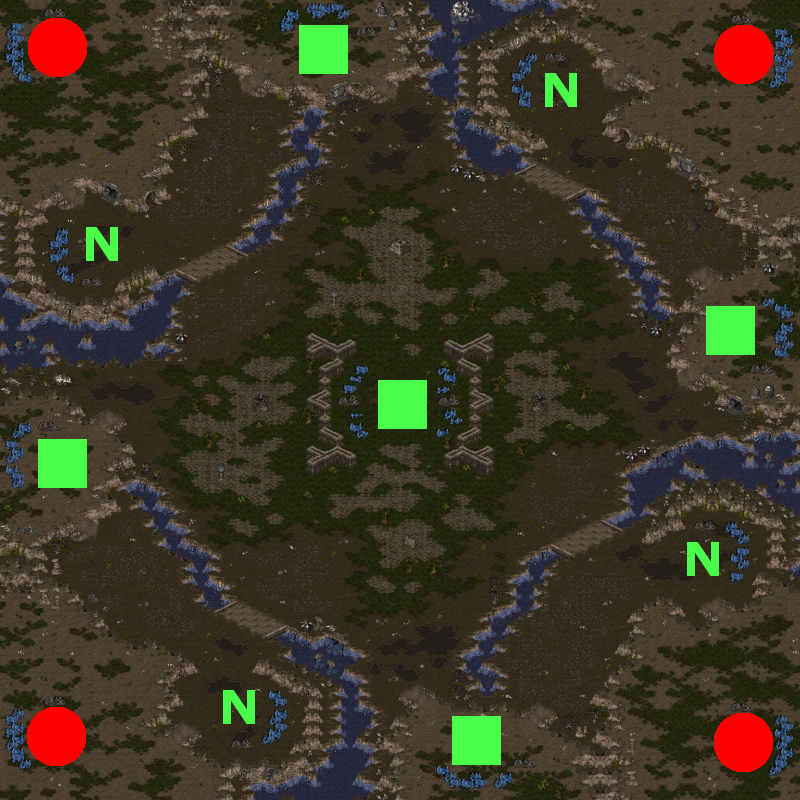
\includegraphics[scale=0.25]{Imagens/FightingSpirit.jpg}}
	\qquad
	\subfloat[Destination] {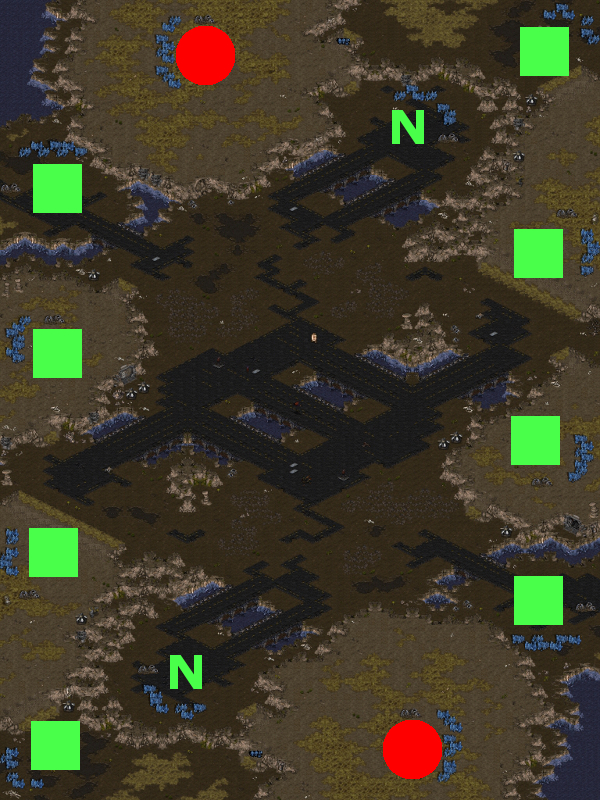
\includegraphics[scale=0.25]{Imagens/Destination.jpg}}
	\caption[Mapas usados nos experimentos.]{Mapas usados nos experimentos. Os c�rculos vermelhos apontam as posi��es iniciais em cada mapa. As naturais est�o marcadas com a letra N. Os quadrados indicam as outras bases.}
	\label{fig:maps}
\end{figure}

Para todos os experimentos, foi usada a trapa�a de invencibilidade\footnote{Esta trapa�a impede que unidades do jogador recebam qualquer tipo de dano proveniente de outros jogadores.}. Isto se deve ao fato da intelig�ncia artificial inimiga atacar o jogador. Caso os ataques fossem bem sucedidos, a perda de trabalhadores ou estruturas criaria ru�dos nos resultados.

Os mapas foram jogados de maneira diferente para verificar cada um dos objetivos deste trabalho. Para testar o sistema de explora��o de recursos, o Cerebrate jogou no mapa Destination e foram criados 17 trabalhadores. A coleta de recursos foi contabilizada durante um per�odo de 5150 quadros, ou aproximadamente tr�s minutos e trinta segundos. Como m�trica, foi utilizada a quantidade total de min�rios coletados ap�s o tempo determinado. O sistema foi comparado com o m�todo padr�o de coleta de recursos do jogo, que � utilizado pelos jogadores profissionais. Desta forma, h� um meio de verificar se o sistema proposto obteve uma melhora tanto na coleta total de recursos como na taxa de min�rios coletados por que o sistema padr�o.

O sistema de posicionamento e constru��o de estruturas foi testado em ambos os mapas. A avalia��o do posicionamento das estruturas se deu atrav�s da cria��o de muralhas nas naturais de todas as posi��es iniciais dos mapas. Utilizaremos a soma de todas as brechas existentes entre as estruturas e do final da muralha at� o ponto n�o naveg�vel mais pr�ximo, como medida de avalia��o. As muralhas alocadas pelo Cerebrate foram comparadas com as muralhas propostas pelo site TeamLiquid\footnote{\url{http://teamliquid.net/}}. Este site re�ne jogadores de diversos n�veis, desde amadores at� jogadores profissionais, para discutir os eventos que acontecem sobre StarCraft. As recomenda��es de muralhas publicadas neste site foram escolhidas por jogadores profissionais e jogadores amadores de alto n�vel, com o objetivo de reduzir as brechas existentes. Al�m de comparar quantitativamente, as muralhas tamb�m foram comparadas qualitativamente.

O sistema de defini��o da sequ�ncia de expans�o territorial foi avaliado tanto em Destination como em Fighting Spirit. Ele foi comparado com as ordens de expans�o usadas por jogadores profissionais nos mesmos mapas. Foram usados, para compara��o, jogos Zerg versus Terran que ocorreram em quatro competi��es:

\begin{itemize}
 	\item WCG Korea 2009\footnote{\url{http://www.teamliquid.net/tlpd/korean/leagues/219_WCG2009_Korea/main}},
 	\item WCG Korea 2010\footnote{\url{http://www.teamliquid.net/tlpd/korean/leagues/596_WCG2010_Korea/main}},
 	\item GOM Classic Season 4\footnote{\url{http://www.teamliquid.net/tlpd/korean/leagues/4329_GOMTV_Classic_Season_4/main}},
 	\item 2010 BigFile MBCGame StarCraft League\footnote{\url{http://www.teamliquid.net/tlpd/korean/leagues/530_Bigfile_MSL/main}}.
 \end{itemize}


Por fim, as aberturas foram testadas em todos os mapas. Foram escolhidas cinco aberturas sugeridas por um jogador de alto n�vel em entrevista. Elas s�o \emph{5 pool}, \emph{9 pool}, \emph{overpool}, \emph{12 pool} e \emph{12 hatch}. As aberturas foram comparadas de acordo com a quantidade de min�rios coletados e o tempo de t�rmino da ordem de constru��o. Tamb�m s�o mostrados os tempos em que os soldados inimigos chegaram � base. O Cerebrate enfrentou em todos os experimentos a \emph{game AI} nativa do jogo. As aberturas est�o descritas atrav�s das ordens de constru��o expostas na Tabela~\ref{tab:bo}.

\begin{table}[h]
	% T�tulo de tabelas sempre aparecem antes da tabela
	\center
	{
		\begin{tabular}{l|l|l|l|l}
			\hline
			\textbf{5 pool} & \textbf{9 pool} & \textbf{Overpool} & \textbf{12 pool} & \textbf{12 hatch}\\
			\hline
			\emph{Drone} & 5 \emph{drones} & 5 \emph{drones} & 5 \emph{drones} & 5 \emph{drones}\\
			\emph{Spawning Pool} & \emph{Spawning Pool} & \emph{Overlord} & \emph{Overlord} & \emph{Overlord}\\
			2 \emph{drones} & \emph{Drone} & \emph{Spawning Pool} & 3 \emph{drones} & 3 \emph{drones}\\
			3 \emph{zerglings} & \emph{Overlord} & \emph{Drone} & \emph{Spawning Pool} & \emph{Hatchery}\\
			& 3 \emph{zerglings} & 3 \emph{zerglings} & \emph{Hatchery} & \emph{Spawning Pool}\\
			& & & 3 \emph{zerglings} & 3 \emph{zerglings}\\
			\hline
		\end{tabular}
	}
	\caption{Ordens de constru��o usadas no confronto Zerg versus Terran.}
	\label{tab:bo}
\end{table}

\section{Coleta de Min�rios}
A Figura~\ref{fig:graph-mingather} mostra os resultados referentes aos min�rios coletados atrav�s da m�quina de estados do Cerebrate bem como a t�cnica implementada pelo jogo. A princ�pio, n�o existem grandes diferen�as entre a quantidade de min�rios coletados, pois existe apenas um trabalhador por min�rio. Esses trabalhadores trabalham de forma id�ntica em ambos os casos. Mas conforme o n�mero de trabalhadores por min�rio aumenta, maior fica a diferen�a entre os min�rios coletados, mostrando que o comportamento conhecido como ``trabalhadores andarilhos'' torna a minera��o mais ineficiente que poderia ser. Esse comportamento acontece quando um trabalhador encontra uma jazida j� sendo minerada. Ele, ent�o, busca outra jazida que esteja livre no quadro atual. Ao final do experimento foram coletados mais de 100 min�rios a mais que o m�todo nativo, em cada caso. Isto mostra que o tempo perdido ao ir de uma jazida � outra pode ser usado esperando a mesma jazida ocupada ficar livre. Para efeito de compara��o, com esses 100 min�rios � poss�vel construir um \emph{overlord}, que aumentaria a capacidade populacional, dois trabalhadores ou quatro \emph{zerglings}.

\begin{figure}[H]
	\centering
	\subfloat[Destination (posi��o superior).] {
		\begin{tikzpicture}
			\begin{axis}[
				width=7.1cm,height=10cm,
				xlabel={\footnotesize{Quadros}},
				ylabel={\footnotesize{Min�rios coletados}},
				xmin=1, ymin = 0,
				xmax=5150, ymax = 2500]

				\addplot[color={patches}] coordinates {
					(1,0) (2,0) (3,0) (4,0) (5,0) (6,0) (7,0) (8,0) (9,0) (10,0) (11,0) (12,0) (13,0) (14,0) (15,0) (16,0) (17,0) (18,0) (19,0) (20,0) (21,0) (22,0) (23,0) (24,0) (25,0) (26,0) (27,0) (28,0) (29,0) (30,0) (31,0) (32,0) (33,0) (34,0) (35,0) (36,0) (37,0) (38,0) (39,0) (40,0) (41,0) (42,0) (43,0) (44,0) (45,0) (46,0) (47,0) (48,0) (49,0) (50,0) (51,0) (52,0) (53,0) (54,0) (55,0) (56,0) (57,0) (58,0) (59,0) (60,0) (61,0) (62,0) (63,0) (64,0) (65,0) (66,0) (67,0) (68,0) (69,0) (70,0) (71,0) (72,0) (73,0) (74,0) (75,0) (76,0) (77,0) (78,0) (79,0) (80,0) (81,0) (82,0) (83,0) (84,0) (85,0) (86,0) (87,0) (88,0) (89,0) (90,0) (91,0) (92,0) (93,0) (94,0) (95,0) (96,0) (97,0) (98,0) (99,0) (100,0) (101,0) (102,0) (103,0) (104,0) (105,0) (106,0) (107,0) (108,0) (109,0) (110,0) (111,0) (112,0) (113,0) (114,0) (115,0) (116,0) (117,0) (118,0) (119,0) (120,0) (121,0) (122,0) (123,0) (124,0) (125,0) (126,0) (127,0) (128,0) (129,0) (130,0) (131,0) (132,0) (133,0) (134,0) (135,0) (136,0) (137,0) (138,0) (139,0) (140,0) (141,0) (142,0) (143,0) (144,0) (145,0) (146,0) (147,0) (148,0) (149,0) (150,0) (151,0) (152,0) (153,0) (154,0) (155,0) (156,0) (157,0) (158,0) (159,0) (160,0) (161,0) (162,0) (163,0) (164,0) (165,0) (166,0) (167,0) (168,0) (169,0) (170,0) (171,0) (172,0) (173,0) (174,0) (175,0) (176,0) (177,0) (178,0) (179,0) (180,8) (181,8) (182,8) (183,8) (184,8) (185,8) (186,8) (187,8) (188,16) (189,16) (190,16) (191,16) (192,16) (193,16) (194,16) (195,16) (196,24) (197,24) (198,24) (199,32) (200,32) (201,32) (202,32) (203,32) (204,32) (205,32) (206,32) (207,32) (208,32) (209,32) (210,32) (211,32) (212,32) (213,32) (214,32) (215,32) (216,32) (217,32) (218,32) (219,32) (220,32) (221,32) (222,32) (223,32) (224,32) (225,32) (226,32) (227,32) (228,32) (229,32) (230,32) (231,32) (232,32) (233,32) (234,32) (235,32) (236,32) (237,32) (238,32) (239,32) (240,32) (241,32) (242,32) (243,32) (244,32) (245,32) (246,32) (247,32) (248,32) (249,32) (250,32) (251,32) (252,32) (253,32) (254,32) (255,32) (256,32) (257,32) (258,32) (259,32) (260,32) (261,32) (262,32) (263,32) (264,32) (265,32) (266,32) (267,32) (268,32) (269,32) (270,32) (271,32) (272,32) (273,32) (274,32) (275,32) (276,32) (277,32) (278,32) (279,32) (280,32) (281,32) (282,32) (283,32) (284,32) (285,32) (286,32) (287,32) (288,32) (289,32) (290,32) (291,32) (292,32) (293,32) (294,32) (295,32) (296,32) (297,32) (298,32) (299,32) (300,32) (301,32) (302,32) (303,32) (304,32) (305,32) (306,32) (307,32) (308,32) (309,32) (310,32) (311,32) (312,32) (313,32) (314,32) (315,32) (316,32) (317,32) (318,32) (319,32) (320,32) (321,32) (322,32) (323,32) (324,32) (325,32) (326,32) (327,32) (328,32) (329,32) (330,32) (331,32) (332,32) (333,32) (334,32) (335,32) (336,32) (337,32) (338,32) (339,40) (340,40) (341,40) (342,40) (343,40) (344,40) (345,40) (346,40) (347,40) (348,40) (349,40) (350,40) (351,40) (352,40) (353,40) (354,40) (355,40) (356,48) (357,56) (358,56) (359,56) (360,56) (361,56) (362,56) (363,56) (364,56) (365,56) (366,56) (367,56) (368,64) (369,64) (370,64) (371,64) (372,64) (373,64) (374,64) (375,64) (376,64) (377,64) (378,64) (379,64) (380,64) (381,64) (382,64) (383,64) (384,64) (385,64) (386,64) (387,64) (388,64) (389,64) (390,64) (391,64) (392,64) (393,64) (394,64) (395,64) (396,64) (397,64) (398,64) (399,64) (400,64) (401,64) (402,64) (403,64) (404,64) (405,64) (406,64) (407,64) (408,64) (409,64) (410,64) (411,64) (412,64) (413,64) (414,64) (415,64) (416,64) (417,64) (418,64) (419,64) (420,64) (421,64) (422,64) (423,64) (424,64) (425,64) (426,64) (427,64) (428,64) (429,64) (430,64) (431,64) (432,64) (433,64) (434,64) (435,64) (436,64) (437,64) (438,64) (439,64) (440,64) (441,64) (442,64) (443,64) (444,64) (445,64) (446,64) (447,64) (448,64) (449,64) (450,64) (451,64) (452,64) (453,64) (454,64) (455,64) (456,64) (457,64) (458,64) (459,64) (460,64) (461,64) (462,64) (463,64) (464,64) (465,64) (466,64) (467,64) (468,64) (469,64) (470,64) (471,64) (472,64) (473,64) (474,64) (475,64) (476,64) (477,64) (478,64) (479,64) (480,64) (481,64) (482,64) (483,64) (484,64) (485,64) (486,64) (487,64) (488,64) (489,64) (490,64) (491,64) (492,64) (493,64) (494,64) (495,64) (496,64) (497,64) (498,64) (499,64) (500,64) (501,72) (502,72) (503,72) (504,72) (505,72) (506,72) (507,72) (508,72) (509,72) (510,72) (511,72) (512,72) (513,72) (514,72) (515,72) (516,72) (517,80) (518,88) (519,88) (520,88) (521,88) (522,88) (523,88) (524,88) (525,88) (526,88) (527,88) (528,88) (529,88) (530,88) (531,88) (532,88) (533,88) (534,88) (535,88) (536,88) (537,88) (538,96) (539,96) (540,96) (541,96) (542,96) (543,96) (544,96) (545,96) (546,96) (547,96) (548,96) (549,96) (550,96) (551,96) (552,96) (553,96) (554,96) (555,96) (556,96) (557,96) (558,96) (559,96) (560,96) (561,96) (562,96) (563,96) (564,96) (565,96) (566,96) (567,96) (568,96) (569,96) (570,96) (571,96) (572,96) (573,96) (574,96) (575,96) (576,96) (577,96) (578,96) (579,96) (580,96) (581,96) (582,96) (583,96) (584,96) (585,96) (586,96) (587,96) (588,96) (589,96) (590,96) (591,96) (592,96) (593,96) (594,96) (595,96) (596,96) (597,96) (598,96) (599,96) (600,96) (601,96) (602,96) (603,96) (604,96) (605,96) (606,96) (607,96) (608,96) (609,96) (610,96) (611,104) (612,104) (613,104) (614,104) (615,104) (616,104) (617,104) (618,104) (619,104) (620,104) (621,104) (622,104) (623,104) (624,104) (625,104) (626,104) (627,104) (628,104) (629,104) (630,104) (631,104) (632,104) (633,104) (634,104) (635,104) (636,104) (637,104) (638,104) (639,104) (640,104) (641,104) (642,104) (643,104) (644,104) (645,104) (646,104) (647,104) (648,104) (649,104) (650,104) (651,104) (652,104) (653,104) (654,104) (655,104) (656,104) (657,104) (658,104) (659,104) (660,112) (661,112) (662,112) (663,112) (664,112) (665,112) (666,112) (667,112) (668,112) (669,112) (670,112) (671,112) (672,112) (673,112) (674,112) (675,112) (676,112) (677,112) (678,112) (679,112) (680,112) (681,112) (682,112) (683,112) (684,112) (685,120) (686,128) (687,128) (688,128) (689,128) (690,128) (691,128) (692,128) (693,128) (694,128) (695,128) (696,128) (697,128) (698,128) (699,128) (700,128) (701,128) (702,128) (703,128) (704,128) (705,128) (706,128) (707,128) (708,128) (709,128) (710,128) (711,128) (712,128) (713,128) (714,128) (715,136) (716,136) (717,136) (718,136) (719,136) (720,136) (721,136) (722,136) (723,136) (724,136) (725,136) (726,136) (727,136) (728,136) (729,136) (730,136) (731,136) (732,136) (733,136) (734,136) (735,136) (736,136) (737,136) (738,136) (739,136) (740,136) (741,136) (742,136) (743,136) (744,136) (745,136) (746,136) (747,136) (748,136) (749,136) (750,136) (751,136) (752,136) (753,136) (754,136) (755,136) (756,136) (757,136) (758,136) (759,136) (760,136) (761,136) (762,136) (763,136) (764,136) (765,136) (766,136) (767,136) (768,136) (769,136) (770,136) (771,136) (772,136) (773,136) (774,136) (775,136) (776,136) (777,136) (778,136) (779,136) (780,136) (781,136) (782,136) (783,136) (784,136) (785,136) (786,136) (787,136) (788,136) (789,136) (790,136) (791,136) (792,136) (793,136) (794,136) (795,136) (796,136) (797,136) (798,136) (799,136) (800,136) (801,136) (802,136) (803,136) (804,136) (805,136) (806,136) (807,136) (808,136) (809,136) (810,136) (811,136) (812,136) (813,144) (814,144) (815,144) (816,144) (817,144) (818,152) (819,152) (820,152) (821,152) (822,152) (823,152) (824,152) (825,152) (826,152) (827,152) (828,152) (829,152) (830,152) (831,152) (832,152) (833,152) (834,152) (835,152) (836,152) (837,152) (838,152) (839,152) (840,152) (841,152) (842,152) (843,152) (844,152) (845,152) (846,160) (847,168) (848,168) (849,168) (850,168) (851,168) (852,168) (853,168) (854,168) (855,168) (856,168) (857,168) (858,168) (859,168) (860,168) (861,168) (862,168) (863,168) (864,168) (865,168) (866,168) (867,168) (868,168) (869,168) (870,168) (871,168) (872,168) (873,168) (874,168) (875,168) (876,168) (877,168) (878,168) (879,168) (880,168) (881,168) (882,168) (883,168) (884,168) (885,168) (886,168) (887,168) (888,176) (889,176) (890,184) (891,184) (892,184) (893,184) (894,184) (895,184) (896,184) (897,184) (898,184) (899,184) (900,184) (901,184) (902,184) (903,184) (904,184) (905,184) (906,184) (907,184) (908,184) (909,184) (910,184) (911,184) (912,184) (913,184) (914,184) (915,184) (916,184) (917,184) (918,184) (919,184) (920,184) (921,184) (922,184) (923,184) (924,184) (925,184) (926,184) (927,184) (928,184) (929,184) (930,184) (931,184) (932,184) (933,184) (934,184) (935,184) (936,184) (937,184) (938,184) (939,184) (940,184) (941,184) (942,184) (943,184) (944,184) (945,184) (946,184) (947,184) (948,184) (949,184) (950,184) (951,184) (952,184) (953,184) (954,184) (955,184) (956,184) (957,184) (958,184) (959,184) (960,184) (961,184) (962,184) (963,184) (964,184) (965,184) (966,192) (967,192) (968,192) (969,192) (970,192) (971,192) (972,192) (973,192) (974,192) (975,192) (976,192) (977,192) (978,192) (979,192) (980,192) (981,192) (982,192) (983,192) (984,192) (985,192) (986,192) (987,192) (988,192) (989,192) (990,200) (991,200) (992,200) (993,200) (994,200) (995,200) (996,200) (997,200) (998,200) (999,200) (1000,200) (1001,200) (1002,200) (1003,200) (1004,200) (1005,200) (1006,200) (1007,200) (1008,200) (1009,208) (1010,216) (1011,216) (1012,216) (1013,216) (1014,216) (1015,216) (1016,216) (1017,216) (1018,216) (1019,216) (1020,216) (1021,216) (1022,216) (1023,216) (1024,216) (1025,216) (1026,216) (1027,216) (1028,216) (1029,216) (1030,216) (1031,216) (1032,216) (1033,216) (1034,216) (1035,216) (1036,216) (1037,216) (1038,216) (1039,216) (1040,216) (1041,216) (1042,216) (1043,216) (1044,216) (1045,216) (1046,216) (1047,216) (1048,216) (1049,216) (1050,216) (1051,216) (1052,216) (1053,216) (1054,216) (1055,216) (1056,216) (1057,216) (1058,216) (1059,216) (1060,216) (1061,216) (1062,224) (1063,224) (1064,232) (1065,232) (1066,232) (1067,232) (1068,232) (1069,232) (1070,232) (1071,232) (1072,232) (1073,232) (1074,232) (1075,232) (1076,232) (1077,232) (1078,232) (1079,232) (1080,232) (1081,232) (1082,232) (1083,232) (1084,232) (1085,232) (1086,232) (1087,232) (1088,232) (1089,232) (1090,232) (1091,232) (1092,232) (1093,232) (1094,232) (1095,232) (1096,232) (1097,232) (1098,232) (1099,232) (1100,232) (1101,232) (1102,232) (1103,232) (1104,232) (1105,232) (1106,232) (1107,232) (1108,232) (1109,232) (1110,232) (1111,232) (1112,232) (1113,232) (1114,232) (1115,232) (1116,232) (1117,232) (1118,232) (1119,232) (1120,232) (1121,232) (1122,232) (1123,232) (1124,232) (1125,240) (1126,240) (1127,240) (1128,240) (1129,240) (1130,240) (1131,240) (1132,240) (1133,240) (1134,240) (1135,240) (1136,240) (1137,240) (1138,240) (1139,240) (1140,240) (1141,240) (1142,240) (1143,240) (1144,240) (1145,240) (1146,240) (1147,240) (1148,240) (1149,240) (1150,240) (1151,240) (1152,240) (1153,240) (1154,240) (1155,240) (1156,240) (1157,240) (1158,240) (1159,240) (1160,240) (1161,240) (1162,240) (1163,240) (1164,240) (1165,240) (1166,240) (1167,248) (1168,248) (1169,248) (1170,248) (1171,248) (1172,248) (1173,248) (1174,248) (1175,248) (1176,248) (1177,256) (1178,264) (1179,264) (1180,264) (1181,264) (1182,264) (1183,272) (1184,272) (1185,272) (1186,272) (1187,272) (1188,272) (1189,272) (1190,272) (1191,272) (1192,272) (1193,272) (1194,272) (1195,272) (1196,272) (1197,272) (1198,272) (1199,272) (1200,272) (1201,272) (1202,272) (1203,272) (1204,272) (1205,272) (1206,272) (1207,272) (1208,272) (1209,272) (1210,272) (1211,272) (1212,272) (1213,272) (1214,272) (1215,272) (1216,272) (1217,272) (1218,272) (1219,272) (1220,272) (1221,272) (1222,272) (1223,272) (1224,272) (1225,272) (1226,272) (1227,272) (1228,272) (1229,272) (1230,272) (1231,272) (1232,280) (1233,280) (1234,280) (1235,280) (1236,280) (1237,280) (1238,280) (1239,280) (1240,280) (1241,280) (1242,280) (1243,280) (1244,288) (1245,288) (1246,288) (1247,288) (1248,288) (1249,288) (1250,288) (1251,288) (1252,288) (1253,288) (1254,288) (1255,288) (1256,288) (1257,288) (1258,288) (1259,288) (1260,288) (1261,288) (1262,288) (1263,288) (1264,288) (1265,288) (1266,288) (1267,288) (1268,288) (1269,288) (1270,288) (1271,288) (1272,288) (1273,288) (1274,288) (1275,288) (1276,288) (1277,296) (1278,296) (1279,296) (1280,296) (1281,296) (1282,296) (1283,296) (1284,296) (1285,296) (1286,296) (1287,296) (1288,296) (1289,296) (1290,296) (1291,296) (1292,296) (1293,296) (1294,296) (1295,296) (1296,296) (1297,296) (1298,296) (1299,296) (1300,296) (1301,296) (1302,296) (1303,296) (1304,296) (1305,296) (1306,296) (1307,296) (1308,296) (1309,296) (1310,296) (1311,296) (1312,296) (1313,296) (1314,296) (1315,296) (1316,296) (1317,296) (1318,296) (1319,296) (1320,296) (1321,296) (1322,296) (1323,296) (1324,296) (1325,296) (1326,296) (1327,296) (1328,296) (1329,296) (1330,296) (1331,296) (1332,296) (1333,296) (1334,296) (1335,296) (1336,296) (1337,296) (1338,296) (1339,304) (1340,312) (1341,320) (1342,320) (1343,320) (1344,320) (1345,320) (1346,320) (1347,320) (1348,320) (1349,320) (1350,320) (1351,320) (1352,320) (1353,320) (1354,320) (1355,320) (1356,320) (1357,320) (1358,320) (1359,320) (1360,320) (1361,320) (1362,320) (1363,320) (1364,328) (1365,328) (1366,328) (1367,328) (1368,336) (1369,336) (1370,336) (1371,336) (1372,336) (1373,336) (1374,336) (1375,336) (1376,336) (1377,336) (1378,336) (1379,336) (1380,336) (1381,336) (1382,336) (1383,336) (1384,336) (1385,336) (1386,336) (1387,336) (1388,336) (1389,336) (1390,336) (1391,336) (1392,336) (1393,336) (1394,336) (1395,336) (1396,336) (1397,336) (1398,336) (1399,336) (1400,336) (1401,336) (1402,336) (1403,336) (1404,336) (1405,336) (1406,336) (1407,336) (1408,336) (1409,336) (1410,344) (1411,344) (1412,344) (1413,352) (1414,352) (1415,352) (1416,352) (1417,352) (1418,352) (1419,352) (1420,352) (1421,352) (1422,352) (1423,352) (1424,352) (1425,352) (1426,352) (1427,352) (1428,352) (1429,352) (1430,352) (1431,352) (1432,352) (1433,352) (1434,352) (1435,352) (1436,360) (1437,360) (1438,360) (1439,360) (1440,360) (1441,360) (1442,360) (1443,360) (1444,360) (1445,360) (1446,360) (1447,360) (1448,360) (1449,360) (1450,360) (1451,360) (1452,360) (1453,360) (1454,360) (1455,360) (1456,360) (1457,360) (1458,360) (1459,360) (1460,360) (1461,360) (1462,360) (1463,360) (1464,360) (1465,360) (1466,360) (1467,360) (1468,360) (1469,360) (1470,360) (1471,360) (1472,360) (1473,360) (1474,360) (1475,360) (1476,360) (1477,360) (1478,360) (1479,360) (1480,360) (1481,360) (1482,360) (1483,360) (1484,360) (1485,360) (1486,360) (1487,360) (1488,360) (1489,360) (1490,360) (1491,360) (1492,360) (1493,360) (1494,360) (1495,360) (1496,360) (1497,360) (1498,360) (1499,368) (1500,376) (1501,376) (1502,376) (1503,376) (1504,376) (1505,376) (1506,376) (1507,384) (1508,384) (1509,384) (1510,384) (1511,384) (1512,384) (1513,384) (1514,384) (1515,384) (1516,384) (1517,384) (1518,384) (1519,384) (1520,384) (1521,384) (1522,384) (1523,384) (1524,384) (1525,384) (1526,392) (1527,392) (1528,392) (1529,400) (1530,400) (1531,400) (1532,400) (1533,400) (1534,400) (1535,400) (1536,400) (1537,400) (1538,400) (1539,400) (1540,400) (1541,400) (1542,400) (1543,400) (1544,400) (1545,400) (1546,400) (1547,400) (1548,400) (1549,400) (1550,400) (1551,400) (1552,400) (1553,400) (1554,400) (1555,400) (1556,408) (1557,408) (1558,408) (1559,408) (1560,408) (1561,408) (1562,408) (1563,408) (1564,408) (1565,408) (1566,408) (1567,408) (1568,408) (1569,408) (1570,408) (1571,408) (1572,408) (1573,408) (1574,408) (1575,408) (1576,408) (1577,408) (1578,408) (1579,408) (1580,408) (1581,416) (1582,416) (1583,424) (1584,424) (1585,424) (1586,424) (1587,424) (1588,432) (1589,432) (1590,432) (1591,432) (1592,432) (1593,432) (1594,432) (1595,432) (1596,432) (1597,432) (1598,432) (1599,432) (1600,432) (1601,432) (1602,432) (1603,432) (1604,432) (1605,432) (1606,432) (1607,432) (1608,432) (1609,432) (1610,432) (1611,432) (1612,432) (1613,432) (1614,432) (1615,432) (1616,432) (1617,432) (1618,432) (1619,432) (1620,432) (1621,432) (1622,432) (1623,432) (1624,432) (1625,432) (1626,432) (1627,432) (1628,432) (1629,432) (1630,432) (1631,432) (1632,432) (1633,432) (1634,432) (1635,432) (1636,432) (1637,432) (1638,432) (1639,432) (1640,432) (1641,432) (1642,432) (1643,432) (1644,432) (1645,432) (1646,432) (1647,432) (1648,432) (1649,432) (1650,432) (1651,432) (1652,432) (1653,432) (1654,432) (1655,432) (1656,432) (1657,432) (1658,432) (1659,432) (1660,432) (1661,432) (1662,432) (1663,440) (1664,448) (1665,448) (1666,448) (1667,448) (1668,448) (1669,448) (1670,448) (1671,448) (1672,448) (1673,448) (1674,448) (1675,448) (1676,448) (1677,448) (1678,448) (1679,448) (1680,448) (1681,448) (1682,448) (1683,448) (1684,448) (1685,448) (1686,448) (1687,448) (1688,448) (1689,456) (1690,456) (1691,456) (1692,456) (1693,456) (1694,464) (1695,464) (1696,464) (1697,464) (1698,464) (1699,464) (1700,464) (1701,464) (1702,464) (1703,464) (1704,464) (1705,464) (1706,472) (1707,472) (1708,472) (1709,472) (1710,472) (1711,472) (1712,472) (1713,472) (1714,472) (1715,472) (1716,472) (1717,472) (1718,472) (1719,472) (1720,472) (1721,472) (1722,472) (1723,472) (1724,472) (1725,472) (1726,472) (1727,472) (1728,472) (1729,472) (1730,472) (1731,472) (1732,472) (1733,472) (1734,480) (1735,480) (1736,480) (1737,480) (1738,480) (1739,480) (1740,480) (1741,480) (1742,480) (1743,480) (1744,480) (1745,480) (1746,480) (1747,488) (1748,488) (1749,488) (1750,488) (1751,488) (1752,488) (1753,488) (1754,488) (1755,488) (1756,488) (1757,488) (1758,496) (1759,496) (1760,504) (1761,504) (1762,504) (1763,504) (1764,504) (1765,504) (1766,504) (1767,504) (1768,504) (1769,504) (1770,504) (1771,504) (1772,504) (1773,504) (1774,504) (1775,504) (1776,504) (1777,504) (1778,504) (1779,504) (1780,504) (1781,504) (1782,504) (1783,504) (1784,504) (1785,504) (1786,504) (1787,504) (1788,504) (1789,504) (1790,504) (1791,504) (1792,504) (1793,504) (1794,504) (1795,504) (1796,504) (1797,504) (1798,504) (1799,504) (1800,504) (1801,504) (1802,504) (1803,504) (1804,504) (1805,504) (1806,504) (1807,504) (1808,504) (1809,504) (1810,504) (1811,504) (1812,504) (1813,504) (1814,504) (1815,504) (1816,504) (1817,504) (1818,504) (1819,504) (1820,504) (1821,504) (1822,504) (1823,504) (1824,504) (1825,504) (1826,504) (1827,504) (1828,504) (1829,504) (1830,504) (1831,504) (1832,512) (1833,520) (1834,520) (1835,520) (1836,520) (1837,520) (1838,520) (1839,520) (1840,520) (1841,520) (1842,520) (1843,520) (1844,520) (1845,520) (1846,520) (1847,520) (1848,520) (1849,520) (1850,520) (1851,520) (1852,520) (1853,520) (1854,520) (1855,520) (1856,520) (1857,520) (1858,520) (1859,528) (1860,528) (1861,528) (1862,528) (1863,528) (1864,536) (1865,536) (1866,536) (1867,536) (1868,536) (1869,536) (1870,536) (1871,536) (1872,536) (1873,536) (1874,536) (1875,536) (1876,544) (1877,544) (1878,544) (1879,544) (1880,544) (1881,544) (1882,544) (1883,544) (1884,544) (1885,544) (1886,544) (1887,544) (1888,544) (1889,544) (1890,544) (1891,544) (1892,544) (1893,544) (1894,544) (1895,544) (1896,544) (1897,544) (1898,544) (1899,552) (1900,552) (1901,552) (1902,552) (1903,560) (1904,560) (1905,560) (1906,560) (1907,560) (1908,560) (1909,560) (1910,560) (1911,560) (1912,560) (1913,560) (1914,560) (1915,560) (1916,560) (1917,560) (1918,560) (1919,560) (1920,560) (1921,560) (1922,560) (1923,560) (1924,560) (1925,560) (1926,560) (1927,568) (1928,568) (1929,568) (1930,568) (1931,568) (1932,568) (1933,568) (1934,568) (1935,568) (1936,568) (1937,568) (1938,576) (1939,576) (1940,576) (1941,576) (1942,576) (1943,576) (1944,576) (1945,576) (1946,576) (1947,576) (1948,576) (1949,576) (1950,576) (1951,576) (1952,576) (1953,576) (1954,576) (1955,576) (1956,576) (1957,576) (1958,576) (1959,576) (1960,576) (1961,576) (1962,576) (1963,576) (1964,576) (1965,576) (1966,576) (1967,576) (1968,576) (1969,576) (1970,576) (1971,576) (1972,576) (1973,576) (1974,576) (1975,576) (1976,576) (1977,576) (1978,576) (1979,576) (1980,576) (1981,576) (1982,576) (1983,576) (1984,576) (1985,576) (1986,576) (1987,576) (1988,576) (1989,576) (1990,576) (1991,576) (1992,576) (1993,576) (1994,576) (1995,576) (1996,576) (1997,576) (1998,576) (1999,576) (2000,584) (2001,592) (2002,592) (2003,592) (2004,592) (2005,592) (2006,592) (2007,592) (2008,592) (2009,592) (2010,592) (2011,592) (2012,592) (2013,592) (2014,592) (2015,592) (2016,592) (2017,592) (2018,592) (2019,592) (2020,592) (2021,592) (2022,592) (2023,592) (2024,592) (2025,592) (2026,592) (2027,592) (2028,592) (2029,592) (2030,592) (2031,592) (2032,592) (2033,592) (2034,592) (2035,592) (2036,600) (2037,600) (2038,600) (2039,600) (2040,600) (2041,608) (2042,608) (2043,608) (2044,608) (2045,608) (2046,608) (2047,608) (2048,608) (2049,608) (2050,608) (2051,608) (2052,608) (2053,616) (2054,616) (2055,616) (2056,616) (2057,616) (2058,624) (2059,624) (2060,624) (2061,624) (2062,624) (2063,624) (2064,624) (2065,624) (2066,624) (2067,624) (2068,624) (2069,624) (2070,624) (2071,624) (2072,624) (2073,624) (2074,624) (2075,624) (2076,624) (2077,624) (2078,624) (2079,624) (2080,632) (2081,632) (2082,632) (2083,632) (2084,632) (2085,632) (2086,632) (2087,632) (2088,632) (2089,632) (2090,632) (2091,632) (2092,632) (2093,632) (2094,632) (2095,632) (2096,632) (2097,632) (2098,632) (2099,632) (2100,632) (2101,632) (2102,632) (2103,632) (2104,632) (2105,632) (2106,640) (2107,640) (2108,640) (2109,640) (2110,640) (2111,640) (2112,640) (2113,640) (2114,640) (2115,640) (2116,640) (2117,640) (2118,640) (2119,640) (2120,640) (2121,648) (2122,648) (2123,648) (2124,648) (2125,648) (2126,648) (2127,648) (2128,648) (2129,648) (2130,648) (2131,648) (2132,648) (2133,648) (2134,648) (2135,648) (2136,648) (2137,648) (2138,648) (2139,648) (2140,648) (2141,648) (2142,648) (2143,648) (2144,648) (2145,648) (2146,648) (2147,648) (2148,648) (2149,648) (2150,648) (2151,648) (2152,648) (2153,648) (2154,648) (2155,648) (2156,648) (2157,648) (2158,648) (2159,648) (2160,648) (2161,656) (2162,656) (2163,664) (2164,664) (2165,664) (2166,664) (2167,664) (2168,664) (2169,664) (2170,664) (2171,664) (2172,664) (2173,664) (2174,664) (2175,664) (2176,664) (2177,664) (2178,664) (2179,664) (2180,664) (2181,664) (2182,664) (2183,664) (2184,664) (2185,664) (2186,664) (2187,664) (2188,664) (2189,664) (2190,664) (2191,664) (2192,664) (2193,664) (2194,664) (2195,664) (2196,664) (2197,664) (2198,664) (2199,664) (2200,664) (2201,664) (2202,664) (2203,664) (2204,664) (2205,672) (2206,672) (2207,672) (2208,672) (2209,680) (2210,688) (2211,688) (2212,688) (2213,688) (2214,688) (2215,688) (2216,688) (2217,688) (2218,688) (2219,688) (2220,688) (2221,688) (2222,696) (2223,696) (2224,696) (2225,696) (2226,696) (2227,696) (2228,696) (2229,696) (2230,696) (2231,696) (2232,696) (2233,696) (2234,696) (2235,696) (2236,696) (2237,696) (2238,696) (2239,696) (2240,696) (2241,696) (2242,696) (2243,696) (2244,696) (2245,696) (2246,696) (2247,696) (2248,696) (2249,696) (2250,696) (2251,696) (2252,696) (2253,696) (2254,696) (2255,696) (2256,696) (2257,696) (2258,696) (2259,696) (2260,696) (2261,696) (2262,696) (2263,704) (2264,704) (2265,704) (2266,704) (2267,704) (2268,704) (2269,704) (2270,704) (2271,704) (2272,704) (2273,704) (2274,704) (2275,704) (2276,704) (2277,704) (2278,712) (2279,712) (2280,712) (2281,712) (2282,712) (2283,712) (2284,712) (2285,712) (2286,712) (2287,712) (2288,712) (2289,712) (2290,712) (2291,712) (2292,712) (2293,712) (2294,712) (2295,712) (2296,712) (2297,712) (2298,720) (2299,720) (2300,720) (2301,720) (2302,720) (2303,720) (2304,720) (2305,720) (2306,720) (2307,720) (2308,720) (2309,720) (2310,720) (2311,720) (2312,720) (2313,720) (2314,720) (2315,720) (2316,720) (2317,720) (2318,720) (2319,720) (2320,720) (2321,720) (2322,720) (2323,720) (2324,720) (2325,720) (2326,720) (2327,720) (2328,720) (2329,728) (2330,728) (2331,736) (2332,736) (2333,736) (2334,736) (2335,736) (2336,736) (2337,736) (2338,736) (2339,736) (2340,736) (2341,736) (2342,736) (2343,736) (2344,736) (2345,736) (2346,736) (2347,736) (2348,736) (2349,736) (2350,736) (2351,736) (2352,736) (2353,736) (2354,736) (2355,736) (2356,736) (2357,736) (2358,736) (2359,736) (2360,736) (2361,736) (2362,736) (2363,736) (2364,736) (2365,736) (2366,736) (2367,736) (2368,744) (2369,744) (2370,744) (2371,744) (2372,744) (2373,744) (2374,744) (2375,744) (2376,744) (2377,744) (2378,744) (2379,744) (2380,744) (2381,744) (2382,752) (2383,752) (2384,752) (2385,752) (2386,752) (2387,760) (2388,760) (2389,760) (2390,760) (2391,760) (2392,760) (2393,760) (2394,760) (2395,760) (2396,760) (2397,760) (2398,760) (2399,760) (2400,760) (2401,768) (2402,768) (2403,768) (2404,768) (2405,768) (2406,768) (2407,768) (2408,768) (2409,768) (2410,768) (2411,768) (2412,768) (2413,768) (2414,768) (2415,768) (2416,768) (2417,768) (2418,768) (2419,768) (2420,768) (2421,768) (2422,768) (2423,768) (2424,768) (2425,768) (2426,768) (2427,768) (2428,768) (2429,768) (2430,768) (2431,768) (2432,768) (2433,768) (2434,768) (2435,768) (2436,768) (2437,768) (2438,768) (2439,768) (2440,768) (2441,768) (2442,768) (2443,768) (2444,768) (2445,768) (2446,768) (2447,768) (2448,768) (2449,768) (2450,768) (2451,776) (2452,776) (2453,784) (2454,784) (2455,784) (2456,784) (2457,784) (2458,784) (2459,784) (2460,784) (2461,784) (2462,784) (2463,784) (2464,784) (2465,784) (2466,784) (2467,784) (2468,784) (2469,792) (2470,792) (2471,792) (2472,792) (2473,792) (2474,792) (2475,792) (2476,792) (2477,792) (2478,792) (2479,792) (2480,792) (2481,792) (2482,792) (2483,792) (2484,792) (2485,792) (2486,792) (2487,792) (2488,792) (2489,792) (2490,792) (2491,800) (2492,808) (2493,808) (2494,808) (2495,808) (2496,808) (2497,808) (2498,808) (2499,808) (2500,808) (2501,808) (2502,808) (2503,808) (2504,808) (2505,808) (2506,808) (2507,808) (2508,808) (2509,808) (2510,808) (2511,808) (2512,808) (2513,808) (2514,808) (2515,808) (2516,808) (2517,808) (2518,808) (2519,808) (2520,816) (2521,816) (2522,816) (2523,816) (2524,816) (2525,816) (2526,816) (2527,816) (2528,816) (2529,816) (2530,816) (2531,816) (2532,816) (2533,816) (2534,816) (2535,816) (2536,816) (2537,816) (2538,816) (2539,816) (2540,816) (2541,824) (2542,824) (2543,824) (2544,824) (2545,824) (2546,824) (2547,824) (2548,824) (2549,824) (2550,824) (2551,824) (2552,824) (2553,824) (2554,824) (2555,832) (2556,832) (2557,832) (2558,832) (2559,832) (2560,832) (2561,832) (2562,832) (2563,832) (2564,832) (2565,832) (2566,832) (2567,832) (2568,832) (2569,832) (2570,832) (2571,832) (2572,832) (2573,832) (2574,840) (2575,840) (2576,840) (2577,840) (2578,840) (2579,840) (2580,840) (2581,840) (2582,840) (2583,840) (2584,840) (2585,840) (2586,848) (2587,848) (2588,848) (2589,848) (2590,848) (2591,848) (2592,848) (2593,848) (2594,848) (2595,848) (2596,848) (2597,848) (2598,848) (2599,848) (2600,848) (2601,848) (2602,848) (2603,848) (2604,848) (2605,848) (2606,848) (2607,848) (2608,848) (2609,848) (2610,848) (2611,848) (2612,848) (2613,848) (2614,848) (2615,848) (2616,848) (2617,848) (2618,848) (2619,856) (2620,856) (2621,856) (2622,856) (2623,856) (2624,856) (2625,856) (2626,856) (2627,856) (2628,856) (2629,856) (2630,856) (2631,856) (2632,864) (2633,864) (2634,864) (2635,864) (2636,864) (2637,872) (2638,872) (2639,872) (2640,880) (2641,880) (2642,880) (2643,880) (2644,880) (2645,880) (2646,880) (2647,880) (2648,880) (2649,880) (2650,880) (2651,880) (2652,880) (2653,888) (2654,896) (2655,896) (2656,896) (2657,896) (2658,896) (2659,896) (2660,896) (2661,896) (2662,896) (2663,896) (2664,896) (2665,896) (2666,896) (2667,896) (2668,896) (2669,896) (2670,896) (2671,896) (2672,896) (2673,896) (2674,896) (2675,896) (2676,896) (2677,896) (2678,896) (2679,896) (2680,896) (2681,896) (2682,896) (2683,896) (2684,896) (2685,896) (2686,896) (2687,896) (2688,896) (2689,896) (2690,896) (2691,896) (2692,896) (2693,896) (2694,896) (2695,896) (2696,896) (2697,896) (2698,896) (2699,896) (2700,896) (2701,896) (2702,896) (2703,896) (2704,896) (2705,896) (2706,896) (2707,896) (2708,896) (2709,896) (2710,896) (2711,896) (2712,896) (2713,896) (2714,904) (2715,904) (2716,904) (2717,904) (2718,904) (2719,904) (2720,912) (2721,912) (2722,912) (2723,912) (2724,912) (2725,912) (2726,912) (2727,912) (2728,912) (2729,912) (2730,912) (2731,912) (2732,912) (2733,920) (2734,920) (2735,920) (2736,920) (2737,920) (2738,920) (2739,928) (2740,928) (2741,928) (2742,928) (2743,928) (2744,936) (2745,936) (2746,936) (2747,936) (2748,936) (2749,936) (2750,936) (2751,936) (2752,936) (2753,936) (2754,936) (2755,936) (2756,936) (2757,936) (2758,936) (2759,936) (2760,936) (2761,936) (2762,936) (2763,936) (2764,936) (2765,936) (2766,936) (2767,936) (2768,936) (2769,936) (2770,936) (2771,936) (2772,936) (2773,936) (2774,936) (2775,936) (2776,936) (2777,936) (2778,936) (2779,936) (2780,936) (2781,936) (2782,936) (2783,944) (2784,944) (2785,944) (2786,944) (2787,944) (2788,944) (2789,944) (2790,944) (2791,944) (2792,944) (2793,944) (2794,944) (2795,944) (2796,944) (2797,944) (2798,944) (2799,944) (2800,944) (2801,952) (2802,952) (2803,952) (2804,952) (2805,952) (2806,960) (2807,960) (2808,960) (2809,968) (2810,968) (2811,968) (2812,968) (2813,976) (2814,976) (2815,976) (2816,976) (2817,976) (2818,976) (2819,976) (2820,976) (2821,976) (2822,976) (2823,976) (2824,976) (2825,976) (2826,976) (2827,976) (2828,976) (2829,976) (2830,976) (2831,976) (2832,976) (2833,976) (2834,976) (2835,976) (2836,976) (2837,976) (2838,976) (2839,976) (2840,976) (2841,976) (2842,976) (2843,976) (2844,976) (2845,976) (2846,976) (2847,976) (2848,976) (2849,976) (2850,976) (2851,976) (2852,984) (2853,984) (2854,984) (2855,984) (2856,984) (2857,984) (2858,984) (2859,984) (2860,984) (2861,984) (2862,984) (2863,984) (2864,984) (2865,984) (2866,984) (2867,984) (2868,984) (2869,984) (2870,984) (2871,984) (2872,984) (2873,984) (2874,984) (2875,984) (2876,984) (2877,984) (2878,984) (2879,984) (2880,984) (2881,992) (2882,992) (2883,992) (2884,992) (2885,992) (2886,992) (2887,992) (2888,992) (2889,992) (2890,992) (2891,992) (2892,992) (2893,992) (2894,992) (2895,1000) (2896,1000) (2897,1000) (2898,1000) (2899,1000) (2900,1000) (2901,1000) (2902,1000) (2903,1008) (2904,1016) (2905,1016) (2906,1016) (2907,1016) (2908,1016) (2909,1016) (2910,1024) (2911,1024) (2912,1024) (2913,1024) (2914,1024) (2915,1032) (2916,1032) (2917,1032) (2918,1032) (2919,1032) (2920,1032) (2921,1032) (2922,1032) (2923,1032) (2924,1032) (2925,1032) (2926,1032) (2927,1032) (2928,1032) (2929,1032) (2930,1032) (2931,1032) (2932,1032) (2933,1032) (2934,1032) (2935,1032) (2936,1032) (2937,1032) (2938,1032) (2939,1032) (2940,1032) (2941,1032) (2942,1032) (2943,1032) (2944,1032) (2945,1032) (2946,1032) (2947,1032) (2948,1032) (2949,1032) (2950,1032) (2951,1032) (2952,1032) (2953,1032) (2954,1032) (2955,1032) (2956,1032) (2957,1032) (2958,1032) (2959,1032) (2960,1032) (2961,1032) (2962,1032) (2963,1032) (2964,1032) (2965,1032) (2966,1032) (2967,1032) (2968,1032) (2969,1032) (2970,1032) (2971,1048) (2972,1048) (2973,1048) (2974,1048) (2975,1048) (2976,1048) (2977,1048) (2978,1048) (2979,1056) (2980,1056) (2981,1056) (2982,1056) (2983,1056) (2984,1056) (2985,1056) (2986,1056) (2987,1056) (2988,1056) (2989,1056) (2990,1056) (2991,1056) (2992,1056) (2993,1056) (2994,1056) (2995,1056) (2996,1056) (2997,1056) (2998,1056) (2999,1056) (3000,1056) (3001,1056) (3002,1056) (3003,1056) (3004,1056) (3005,1056) (3006,1056) (3007,1056) (3008,1056) (3009,1056) (3010,1056) (3011,1056) (3012,1056) (3013,1056) (3014,1056) (3015,1064) (3016,1064) (3017,1064) (3018,1064) (3019,1064) (3020,1072) (3021,1072) (3022,1072) (3023,1072) (3024,1072) (3025,1072) (3026,1072) (3027,1072) (3028,1072) (3029,1072) (3030,1072) (3031,1072) (3032,1072) (3033,1072) (3034,1072) (3035,1072) (3036,1072) (3037,1080) (3038,1080) (3039,1080) (3040,1080) (3041,1080) (3042,1088) (3043,1088) (3044,1088) (3045,1088) (3046,1088) (3047,1088) (3048,1088) (3049,1088) (3050,1088) (3051,1088) (3052,1088) (3053,1088) (3054,1088) (3055,1088) (3056,1088) (3057,1088) (3058,1088) (3059,1088) (3060,1088) (3061,1088) (3062,1088) (3063,1096) (3064,1104) (3065,1104) (3066,1104) (3067,1104) (3068,1104) (3069,1104) (3070,1104) (3071,1104) (3072,1104) (3073,1104) (3074,1104) (3075,1104) (3076,1104) (3077,1104) (3078,1104) (3079,1104) (3080,1104) (3081,1104) (3082,1104) (3083,1104) (3084,1104) (3085,1104) (3086,1104) (3087,1104) (3088,1104) (3089,1104) (3090,1104) (3091,1104) (3092,1104) (3093,1112) (3094,1112) (3095,1112) (3096,1112) (3097,1112) (3098,1112) (3099,1112) (3100,1112) (3101,1120) (3102,1120) (3103,1120) (3104,1120) (3105,1120) (3106,1120) (3107,1120) (3108,1120) (3109,1120) (3110,1120) (3111,1120) (3112,1120) (3113,1120) (3114,1120) (3115,1120) (3116,1120) (3117,1120) (3118,1120) (3119,1120) (3120,1120) (3121,1120) (3122,1120) (3123,1120) (3124,1120) (3125,1120) (3126,1120) (3127,1120) (3128,1120) (3129,1120) (3130,1120) (3131,1120) (3132,1120) (3133,1120) (3134,1120) (3135,1120) (3136,1120) (3137,1120) (3138,1128) (3139,1128) (3140,1128) (3141,1128) (3142,1128) (3143,1128) (3144,1128) (3145,1128) (3146,1128) (3147,1128) (3148,1128) (3149,1128) (3150,1136) (3151,1144) (3152,1152) (3153,1152) (3154,1152) (3155,1152) (3156,1152) (3157,1152) (3158,1152) (3159,1152) (3160,1152) (3161,1152) (3162,1152) (3163,1152) (3164,1152) (3165,1152) (3166,1152) (3167,1152) (3168,1152) (3169,1152) (3170,1152) (3171,1152) (3172,1152) (3173,1152) (3174,1152) (3175,1152) (3176,1152) (3177,1152) (3178,1152) (3179,1152) (3180,1152) (3181,1152) (3182,1152) (3183,1152) (3184,1152) (3185,1160) (3186,1168) (3187,1168) (3188,1168) (3189,1168) (3190,1176) (3191,1176) (3192,1176) (3193,1176) (3194,1176) (3195,1176) (3196,1176) (3197,1176) (3198,1176) (3199,1176) (3200,1176) (3201,1176) (3202,1176) (3203,1176) (3204,1176) (3205,1176) (3206,1176) (3207,1176) (3208,1176) (3209,1176) (3210,1176) (3211,1176) (3212,1176) (3213,1176) (3214,1176) (3215,1176) (3216,1176) (3217,1184) (3218,1184) (3219,1184) (3220,1184) (3221,1184) (3222,1184) (3223,1192) (3224,1192) (3225,1192) (3226,1192) (3227,1192) (3228,1192) (3229,1192) (3230,1192) (3231,1192) (3232,1192) (3233,1192) (3234,1192) (3235,1192) (3236,1192) (3237,1192) (3238,1192) (3239,1192) (3240,1192) (3241,1192) (3242,1192) (3243,1192) (3244,1192) (3245,1192) (3246,1192) (3247,1192) (3248,1192) (3249,1192) (3250,1192) (3251,1192) (3252,1192) (3253,1192) (3254,1192) (3255,1192) (3256,1192) (3257,1192) (3258,1192) (3259,1192) (3260,1192) (3261,1192) (3262,1192) (3263,1200) (3264,1200) (3265,1200) (3266,1200) (3267,1200) (3268,1200) (3269,1200) (3270,1200) (3271,1200) (3272,1200) (3273,1200) (3274,1200) (3275,1200) (3276,1200) (3277,1200) (3278,1200) (3279,1200) (3280,1200) (3281,1200) (3282,1200) (3283,1200) (3284,1200) (3285,1200) (3286,1200) (3287,1200) (3288,1200) (3289,1208) (3290,1208) (3291,1208) (3292,1208) (3293,1208) (3294,1208) (3295,1208) (3296,1208) (3297,1208) (3298,1216) (3299,1216) (3300,1216) (3301,1216) (3302,1216) (3303,1216) (3304,1216) (3305,1216) (3306,1216) (3307,1216) (3308,1216) (3309,1216) (3310,1216) (3311,1216) (3312,1216) (3313,1216) (3314,1216) (3315,1216) (3316,1216) (3317,1216) (3318,1216) (3319,1216) (3320,1216) (3321,1216) (3322,1216) (3323,1216) (3324,1216) (3325,1216) (3326,1216) (3327,1216) (3328,1216) (3329,1216) (3330,1224) (3331,1224) (3332,1232) (3333,1232) (3334,1232) (3335,1240) (3336,1248) (3337,1248) (3338,1248) (3339,1248) (3340,1248) (3341,1248) (3342,1256) (3343,1256) (3344,1256) (3345,1256) (3346,1256) (3347,1256) (3348,1256) (3349,1256) (3350,1256) (3351,1256) (3352,1256) (3353,1256) (3354,1256) (3355,1256) (3356,1264) (3357,1264) (3358,1264) (3359,1264) (3360,1272) (3361,1272) (3362,1272) (3363,1272) (3364,1272) (3365,1272) (3366,1272) (3367,1272) (3368,1272) (3369,1272) (3370,1272) (3371,1272) (3372,1272) (3373,1272) (3374,1272) (3375,1272) (3376,1272) (3377,1272) (3378,1272) (3379,1272) (3380,1272) (3381,1272) (3382,1272) (3383,1272) (3384,1272) (3385,1272) (3386,1272) (3387,1272) (3388,1272) (3389,1272) (3390,1272) (3391,1272) (3392,1272) (3393,1272) (3394,1272) (3395,1280) (3396,1280) (3397,1280) (3398,1280) (3399,1280) (3400,1280) (3401,1280) (3402,1280) (3403,1280) (3404,1280) (3405,1280) (3406,1280) (3407,1280) (3408,1280) (3409,1280) (3410,1280) (3411,1280) (3412,1280) (3413,1280) (3414,1280) (3415,1280) (3416,1280) (3417,1280) (3418,1280) (3419,1280) (3420,1280) (3421,1280) (3422,1280) (3423,1280) (3424,1280) (3425,1280) (3426,1280) (3427,1280) (3428,1280) (3429,1280) (3430,1280) (3431,1280) (3432,1288) (3433,1288) (3434,1288) (3435,1288) (3436,1288) (3437,1288) (3438,1288) (3439,1296) (3440,1296) (3441,1296) (3442,1296) (3443,1296) (3444,1296) (3445,1296) (3446,1296) (3447,1296) (3448,1296) (3449,1296) (3450,1296) (3451,1296) (3452,1296) (3453,1296) (3454,1296) (3455,1296) (3456,1296) (3457,1296) (3458,1296) (3459,1296) (3460,1296) (3461,1296) (3462,1296) (3463,1296) (3464,1296) (3465,1296) (3466,1296) (3467,1296) (3468,1296) (3469,1296) (3470,1296) (3471,1296) (3472,1296) (3473,1296) (3474,1296) (3475,1296) (3476,1296) (3477,1296) (3478,1296) (3479,1296) (3480,1304) (3481,1304) (3482,1312) (3483,1312) (3484,1312) (3485,1312) (3486,1312) (3487,1312) (3488,1312) (3489,1312) (3490,1312) (3491,1312) (3492,1312) (3493,1312) (3494,1312) (3495,1312) (3496,1312) (3497,1312) (3498,1312) (3499,1312) (3500,1312) (3501,1312) (3502,1312) (3503,1312) (3504,1312) (3505,1312) (3506,1312) (3507,1320) (3508,1320) (3509,1320) (3510,1320) (3511,1328) (3512,1328) (3513,1328) (3514,1328) (3515,1328) (3516,1328) (3517,1336) (3518,1336) (3519,1336) (3520,1336) (3521,1336) (3522,1336) (3523,1344) (3524,1352) (3525,1352) (3526,1352) (3527,1360) (3528,1360) (3529,1360) (3530,1360) (3531,1360) (3532,1360) (3533,1360) (3534,1360) (3535,1360) (3536,1360) (3537,1360) (3538,1360) (3539,1360) (3540,1360) (3541,1360) (3542,1360) (3543,1360) (3544,1360) (3545,1360) (3546,1360) (3547,1360) (3548,1360) (3549,1360) (3550,1360) (3551,1360) (3552,1360) (3553,1360) (3554,1360) (3555,1360) (3556,1360) (3557,1360) (3558,1360) (3559,1360) (3560,1360) (3561,1360) (3562,1360) (3563,1360) (3564,1360) (3565,1360) (3566,1360) (3567,1360) (3568,1360) (3569,1360) (3570,1360) (3571,1360) (3572,1360) (3573,1360) (3574,1360) (3575,1360) (3576,1368) (3577,1368) (3578,1368) (3579,1368) (3580,1368) (3581,1368) (3582,1368) (3583,1368) (3584,1368) (3585,1368) (3586,1376) (3587,1376) (3588,1376) (3589,1376) (3590,1376) (3591,1376) (3592,1376) (3593,1376) (3594,1376) (3595,1376) (3596,1376) (3597,1376) (3598,1376) (3599,1376) (3600,1376) (3601,1376) (3602,1376) (3603,1376) (3604,1376) (3605,1376) (3606,1376) (3607,1376) (3608,1376) (3609,1376) (3610,1376) (3611,1376) (3612,1384) (3613,1384) (3614,1384) (3615,1384) (3616,1384) (3617,1392) (3618,1392) (3619,1392) (3620,1392) (3621,1400) (3622,1400) (3623,1400) (3624,1400) (3625,1400) (3626,1400) (3627,1400) (3628,1400) (3629,1400) (3630,1400) (3631,1400) (3632,1400) (3633,1400) (3634,1400) (3635,1400) (3636,1400) (3637,1400) (3638,1400) (3639,1400) (3640,1400) (3641,1400) (3642,1400) (3643,1400) (3644,1400) (3645,1400) (3646,1400) (3647,1400) (3648,1400) (3649,1400) (3650,1400) (3651,1400) (3652,1400) (3653,1400) (3654,1400) (3655,1400) (3656,1400) (3657,1400) (3658,1400) (3659,1400) (3660,1400) (3661,1400) (3662,1400) (3663,1400) (3664,1400) (3665,1400) (3666,1400) (3667,1400) (3668,1400) (3669,1400) (3670,1408) (3671,1408) (3672,1416) (3673,1416) (3674,1416) (3675,1416) (3676,1416) (3677,1416) (3678,1416) (3679,1416) (3680,1416) (3681,1416) (3682,1416) (3683,1416) (3684,1416) (3685,1416) (3686,1416) (3687,1416) (3688,1424) (3689,1424) (3690,1424) (3691,1424) (3692,1424) (3693,1424) (3694,1424) (3695,1432) (3696,1432) (3697,1432) (3698,1432) (3699,1440) (3700,1440) (3701,1440) (3702,1440) (3703,1440) (3704,1440) (3705,1440) (3706,1440) (3707,1440) (3708,1440) (3709,1440) (3710,1448) (3711,1448) (3712,1448) (3713,1448) (3714,1448) (3715,1448) (3716,1448) (3717,1448) (3718,1448) (3719,1448) (3720,1448) (3721,1456) (3722,1456) (3723,1456) (3724,1456) (3725,1456) (3726,1456) (3727,1456) (3728,1456) (3729,1456) (3730,1456) (3731,1456) (3732,1456) (3733,1456) (3734,1464) (3735,1464) (3736,1464) (3737,1464) (3738,1464) (3739,1464) (3740,1464) (3741,1464) (3742,1464) (3743,1464) (3744,1464) (3745,1464) (3746,1464) (3747,1464) (3748,1464) (3749,1464) (3750,1464) (3751,1464) (3752,1464) (3753,1472) (3754,1472) (3755,1472) (3756,1472) (3757,1472) (3758,1472) (3759,1472) (3760,1472) (3761,1472) (3762,1480) (3763,1480) (3764,1480) (3765,1480) (3766,1480) (3767,1480) (3768,1480) (3769,1480) (3770,1480) (3771,1480) (3772,1480) (3773,1480) (3774,1488) (3775,1488) (3776,1488) (3777,1488) (3778,1488) (3779,1488) (3780,1488) (3781,1488) (3782,1488) (3783,1488) (3784,1488) (3785,1488) (3786,1496) (3787,1496) (3788,1496) (3789,1496) (3790,1504) (3791,1504) (3792,1504) (3793,1504) (3794,1504) (3795,1504) (3796,1504) (3797,1504) (3798,1504) (3799,1504) (3800,1504) (3801,1504) (3802,1504) (3803,1504) (3804,1504) (3805,1504) (3806,1504) (3807,1504) (3808,1504) (3809,1504) (3810,1504) (3811,1504) (3812,1504) (3813,1504) (3814,1504) (3815,1504) (3816,1504) (3817,1504) (3818,1504) (3819,1504) (3820,1504) (3821,1504) (3822,1512) (3823,1512) (3824,1512) (3825,1512) (3826,1512) (3827,1512) (3828,1512) (3829,1512) (3830,1512) (3831,1512) (3832,1512) (3833,1512) (3834,1512) (3835,1512) (3836,1512) (3837,1512) (3838,1512) (3839,1512) (3840,1512) (3841,1520) (3842,1520) (3843,1520) (3844,1520) (3845,1520) (3846,1520) (3847,1520) (3848,1520) (3849,1520) (3850,1520) (3851,1520) (3852,1520) (3853,1520) (3854,1520) (3855,1520) (3856,1520) (3857,1520) (3858,1528) (3859,1528) (3860,1528) (3861,1528) (3862,1528) (3863,1528) (3864,1536) (3865,1536) (3866,1536) (3867,1536) (3868,1536) (3869,1536) (3870,1536) (3871,1544) (3872,1552) (3873,1552) (3874,1552) (3875,1552) (3876,1552) (3877,1560) (3878,1560) (3879,1568) (3880,1568) (3881,1568) (3882,1568) (3883,1568) (3884,1568) (3885,1568) (3886,1568) (3887,1568) (3888,1568) (3889,1568) (3890,1568) (3891,1568) (3892,1568) (3893,1568) (3894,1568) (3895,1568) (3896,1568) (3897,1568) (3898,1568) (3899,1568) (3900,1568) (3901,1576) (3902,1576) (3903,1576) (3904,1584) (3905,1584) (3906,1584) (3907,1584) (3908,1584) (3909,1584) (3910,1584) (3911,1584) (3912,1584) (3913,1584) (3914,1584) (3915,1584) (3916,1584) (3917,1584) (3918,1584) (3919,1584) (3920,1584) (3921,1584) (3922,1584) (3923,1584) (3924,1584) (3925,1584) (3926,1584) (3927,1592) (3928,1592) (3929,1592) (3930,1592) (3931,1592) (3932,1592) (3933,1592) (3934,1592) (3935,1592) (3936,1592) (3937,1592) (3938,1592) (3939,1592) (3940,1592) (3941,1592) (3942,1592) (3943,1592) (3944,1592) (3945,1592) (3946,1592) (3947,1592) (3948,1592) (3949,1592) (3950,1592) (3951,1592) (3952,1592) (3953,1592) (3954,1600) (3955,1600) (3956,1600) (3957,1600) (3958,1600) (3959,1600) (3960,1600) (3961,1600) (3962,1600) (3963,1600) (3964,1600) (3965,1600) (3966,1600) (3967,1600) (3968,1600) (3969,1600) (3970,1600) (3971,1600) (3972,1600) (3973,1600) (3974,1600) (3975,1608) (3976,1608) (3977,1608) (3978,1608) (3979,1608) (3980,1608) (3981,1608) (3982,1608) (3983,1608) (3984,1608) (3985,1608) (3986,1608) (3987,1608) (3988,1608) (3989,1608) (3990,1608) (3991,1608) (3992,1608) (3993,1608) (3994,1616) (3995,1616) (3996,1616) (3997,1616) (3998,1616) (3999,1616) (4000,1616) (4001,1616) (4002,1616) (4003,1616) (4004,1616) (4005,1616) (4006,1616) (4007,1616) (4008,1616) (4009,1616) (4010,1616) (4011,1616) (4012,1616) (4013,1616) (4014,1616) (4015,1616) (4016,1616) (4017,1616) (4018,1616) (4019,1616) (4020,1616) (4021,1616) (4022,1632) (4023,1632) (4024,1632) (4025,1632) (4026,1632) (4027,1632) (4028,1632) (4029,1632) (4030,1632) (4031,1632) (4032,1632) (4033,1632) (4034,1632) (4035,1632) (4036,1632) (4037,1640) (4038,1640) (4039,1648) (4040,1648) (4041,1648) (4042,1648) (4043,1648) (4044,1648) (4045,1648) (4046,1648) (4047,1648) (4048,1648) (4049,1648) (4050,1648) (4051,1648) (4052,1648) (4053,1648) (4054,1648) (4055,1648) (4056,1648) (4057,1648) (4058,1656) (4059,1656) (4060,1656) (4061,1656) (4062,1656) (4063,1656) (4064,1664) (4065,1664) (4066,1664) (4067,1664) (4068,1664) (4069,1664) (4070,1664) (4071,1664) (4072,1664) (4073,1664) (4074,1664) (4075,1664) (4076,1664) (4077,1664) (4078,1672) (4079,1672) (4080,1672) (4081,1672) (4082,1672) (4083,1672) (4084,1672) (4085,1672) (4086,1672) (4087,1672) (4088,1672) (4089,1672) (4090,1672) (4091,1672) (4092,1672) (4093,1672) (4094,1672) (4095,1672) (4096,1672) (4097,1672) (4098,1672) (4099,1672) (4100,1672) (4101,1672) (4102,1672) (4103,1672) (4104,1672) (4105,1672) (4106,1672) (4107,1672) (4108,1672) (4109,1672) (4110,1672) (4111,1672) (4112,1672) (4113,1672) (4114,1672) (4115,1672) (4116,1672) (4117,1672) (4118,1672) (4119,1672) (4120,1672) (4121,1672) (4122,1672) (4123,1680) (4124,1680) (4125,1680) (4126,1680) (4127,1680) (4128,1680) (4129,1680) (4130,1680) (4131,1680) (4132,1680) (4133,1688) (4134,1688) (4135,1688) (4136,1688) (4137,1688) (4138,1688) (4139,1688) (4140,1688) (4141,1688) (4142,1696) (4143,1696) (4144,1696) (4145,1704) (4146,1704) (4147,1704) (4148,1704) (4149,1704) (4150,1704) (4151,1704) (4152,1704) (4153,1712) (4154,1720) (4155,1720) (4156,1720) (4157,1720) (4158,1720) (4159,1720) (4160,1720) (4161,1720) (4162,1720) (4163,1720) (4164,1720) (4165,1720) (4166,1720) (4167,1720) (4168,1720) (4169,1720) (4170,1720) (4171,1720) (4172,1720) (4173,1720) (4174,1720) (4175,1720) (4176,1720) (4177,1720) (4178,1720) (4179,1720) (4180,1720) (4181,1720) (4182,1720) (4183,1720) (4184,1720) (4185,1720) (4186,1720) (4187,1720) (4188,1720) (4189,1720) (4190,1720) (4191,1720) (4192,1720) (4193,1720) (4194,1720) (4195,1720) (4196,1720) (4197,1720) (4198,1720) (4199,1720) (4200,1720) (4201,1720) (4202,1720) (4203,1720) (4204,1720) (4205,1720) (4206,1720) (4207,1720) (4208,1720) (4209,1720) (4210,1728) (4211,1728) (4212,1728) (4213,1728) (4214,1728) (4215,1736) (4216,1736) (4217,1736) (4218,1736) (4219,1736) (4220,1744) (4221,1744) (4222,1744) (4223,1744) (4224,1744) (4225,1744) (4226,1744) (4227,1744) (4228,1744) (4229,1744) (4230,1752) (4231,1752) (4232,1752) (4233,1752) (4234,1752) (4235,1752) (4236,1752) (4237,1760) (4238,1760) (4239,1760) (4240,1768) (4241,1768) (4242,1768) (4243,1768) (4244,1768) (4245,1768) (4246,1768) (4247,1768) (4248,1768) (4249,1768) (4250,1768) (4251,1768) (4252,1768) (4253,1768) (4254,1768) (4255,1768) (4256,1768) (4257,1768) (4258,1768) (4259,1768) (4260,1768) (4261,1768) (4262,1768) (4263,1768) (4264,1768) (4265,1768) (4266,1768) (4267,1768) (4268,1768) (4269,1768) (4270,1768) (4271,1768) (4272,1768) (4273,1768) (4274,1768) (4275,1768) (4276,1768) (4277,1768) (4278,1768) (4279,1768) (4280,1768) (4281,1768) (4282,1768) (4283,1768) (4284,1768) (4285,1768) (4286,1768) (4287,1768) (4288,1768) (4289,1768) (4290,1768) (4291,1768) (4292,1768) (4293,1768) (4294,1768) (4295,1768) (4296,1776) (4297,1776) (4298,1776) (4299,1776) (4300,1776) (4301,1776) (4302,1776) (4303,1776) (4304,1776) (4305,1776) (4306,1776) (4307,1776) (4308,1776) (4309,1784) (4310,1784) (4311,1784) (4312,1784) (4313,1784) (4314,1792) (4315,1792) (4316,1792) (4317,1792) (4318,1792) (4319,1800) (4320,1800) (4321,1800) (4322,1800) (4323,1800) (4324,1800) (4325,1800) (4326,1808) (4327,1816) (4328,1816) (4329,1816) (4330,1816) (4331,1816) (4332,1816) (4333,1816) (4334,1816) (4335,1816) (4336,1816) (4337,1816) (4338,1816) (4339,1816) (4340,1816) (4341,1816) (4342,1816) (4343,1816) (4344,1816) (4345,1816) (4346,1816) (4347,1816) (4348,1816) (4349,1816) (4350,1816) (4351,1816) (4352,1816) (4353,1816) (4354,1816) (4355,1816) (4356,1816) (4357,1816) (4358,1816) (4359,1816) (4360,1816) (4361,1816) (4362,1816) (4363,1816) (4364,1824) (4365,1824) (4366,1824) (4367,1824) (4368,1824) (4369,1824) (4370,1824) (4371,1824) (4372,1824) (4373,1824) (4374,1824) (4375,1824) (4376,1824) (4377,1824) (4378,1824) (4379,1824) (4380,1824) (4381,1824) (4382,1824) (4383,1824) (4384,1824) (4385,1824) (4386,1824) (4387,1824) (4388,1824) (4389,1824) (4390,1832) (4391,1832) (4392,1840) (4393,1840) (4394,1840) (4395,1840) (4396,1840) (4397,1840) (4398,1840) (4399,1840) (4400,1840) (4401,1840) (4402,1840) (4403,1840) (4404,1840) (4405,1840) (4406,1840) (4407,1840) (4408,1840) (4409,1840) (4410,1840) (4411,1840) (4412,1840) (4413,1840) (4414,1840) (4415,1848) (4416,1848) (4417,1848) (4418,1856) (4419,1856) (4420,1856) (4421,1856) (4422,1856) (4423,1864) (4424,1872) (4425,1872) (4426,1872) (4427,1872) (4428,1872) (4429,1872) (4430,1872) (4431,1872) (4432,1872) (4433,1872) (4434,1872) (4435,1872) (4436,1872) (4437,1872) (4438,1872) (4439,1872) (4440,1872) (4441,1872) (4442,1872) (4443,1872) (4444,1872) (4445,1872) (4446,1872) (4447,1872) (4448,1872) (4449,1872) (4450,1872) (4451,1872) (4452,1872) (4453,1872) (4454,1872) (4455,1872) (4456,1872) (4457,1872) (4458,1872) (4459,1872) (4460,1872) (4461,1872) (4462,1872) (4463,1872) (4464,1872) (4465,1872) (4466,1872) (4467,1872) (4468,1872) (4469,1880) (4470,1880) (4471,1880) (4472,1880) (4473,1888) (4474,1888) (4475,1888) (4476,1888) (4477,1888) (4478,1888) (4479,1888) (4480,1888) (4481,1888) (4482,1888) (4483,1888) (4484,1888) (4485,1888) (4486,1896) (4487,1896) (4488,1896) (4489,1896) (4490,1896) (4491,1896) (4492,1896) (4493,1896) (4494,1896) (4495,1896) (4496,1896) (4497,1896) (4498,1896) (4499,1896) (4500,1896) (4501,1896) (4502,1896) (4503,1896) (4504,1896) (4505,1904) (4506,1912) (4507,1912) (4508,1912) (4509,1912) (4510,1912) (4511,1912) (4512,1912) (4513,1912) (4514,1912) (4515,1912) (4516,1912) (4517,1912) (4518,1912) (4519,1912) (4520,1912) (4521,1912) (4522,1912) (4523,1912) (4524,1912) (4525,1912) (4526,1912) (4527,1912) (4528,1912) (4529,1912) (4530,1912) (4531,1912) (4532,1912) (4533,1912) (4534,1912) (4535,1912) (4536,1912) (4537,1912) (4538,1920) (4539,1920) (4540,1920) (4541,1920) (4542,1920) (4543,1920) (4544,1920) (4545,1920) (4546,1920) (4547,1920) (4548,1920) (4549,1928) (4550,1928) (4551,1928) (4552,1928) (4553,1928) (4554,1928) (4555,1928) (4556,1928) (4557,1928) (4558,1928) (4559,1928) (4560,1936) (4561,1936) (4562,1936) (4563,1944) (4564,1944) (4565,1944) (4566,1944) (4567,1944) (4568,1944) (4569,1944) (4570,1944) (4571,1944) (4572,1944) (4573,1944) (4574,1944) (4575,1944) (4576,1944) (4577,1944) (4578,1944) (4579,1944) (4580,1944) (4581,1944) (4582,1944) (4583,1952) (4584,1952) (4585,1952) (4586,1952) (4587,1960) (4588,1960) (4589,1960) (4590,1960) (4591,1960) (4592,1960) (4593,1960) (4594,1968) (4595,1968) (4596,1968) (4597,1968) (4598,1968) (4599,1968) (4600,1968) (4601,1968) (4602,1976) (4603,1976) (4604,1976) (4605,1976) (4606,1976) (4607,1976) (4608,1976) (4609,1976) (4610,1976) (4611,1976) (4612,1976) (4613,1976) (4614,1976) (4615,1976) (4616,1976) (4617,1976) (4618,1976) (4619,1976) (4620,1976) (4621,1976) (4622,1976) (4623,1976) (4624,1976) (4625,1976) (4626,1976) (4627,1976) (4628,1976) (4629,1976) (4630,1976) (4631,1976) (4632,1976) (4633,1984) (4634,1984) (4635,1984) (4636,1984) (4637,1984) (4638,1984) (4639,1984) (4640,1984) (4641,1984) (4642,1984) (4643,1984) (4644,1992) (4645,1992) (4646,1992) (4647,1992) (4648,1992) (4649,2000) (4650,2000) (4651,2000) (4652,2000) (4653,2000) (4654,2000) (4655,2000) (4656,2000) (4657,2000) (4658,2000) (4659,2000) (4660,2000) (4661,2000) (4662,2000) (4663,2000) (4664,2000) (4665,2000) (4666,2000) (4667,2000) (4668,2000) (4669,2008) (4670,2008) (4671,2008) (4672,2008) (4673,2008) (4674,2008) (4675,2008) (4676,2008) (4677,2008) (4678,2008) (4679,2008) (4680,2016) (4681,2016) (4682,2016) (4683,2016) (4684,2016) (4685,2016) (4686,2016) (4687,2016) (4688,2016) (4689,2016) (4690,2016) (4691,2016) (4692,2016) (4693,2016) (4694,2016) (4695,2016) (4696,2016) (4697,2016) (4698,2016) (4699,2016) (4700,2016) (4701,2016) (4702,2016) (4703,2016) (4704,2016) (4705,2016) (4706,2016) (4707,2016) (4708,2016) (4709,2016) (4710,2016) (4711,2016) (4712,2016) (4713,2016) (4714,2016) (4715,2016) (4716,2016) (4717,2016) (4718,2016) (4719,2024) (4720,2024) (4721,2024) (4722,2024) (4723,2024) (4724,2024) (4725,2024) (4726,2024) (4727,2024) (4728,2024) (4729,2024) (4730,2024) (4731,2024) (4732,2024) (4733,2024) (4734,2032) (4735,2032) (4736,2040) (4737,2040) (4738,2040) (4739,2040) (4740,2040) (4741,2048) (4742,2048) (4743,2048) (4744,2048) (4745,2048) (4746,2048) (4747,2048) (4748,2048) (4749,2048) (4750,2048) (4751,2048) (4752,2048) (4753,2048) (4754,2048) (4755,2048) (4756,2048) (4757,2048) (4758,2048) (4759,2056) (4760,2056) (4761,2056) (4762,2056) (4763,2072) (4764,2072) (4765,2072) (4766,2072) (4767,2072) (4768,2072) (4769,2072) (4770,2072) (4771,2072) (4772,2072) (4773,2072) (4774,2072) (4775,2072) (4776,2072) (4777,2072) (4778,2072) (4779,2072) (4780,2072) (4781,2072) (4782,2080) (4783,2080) (4784,2080) (4785,2080) (4786,2080) (4787,2080) (4788,2080) (4789,2080) (4790,2080) (4791,2080) (4792,2080) (4793,2080) (4794,2080) (4795,2080) (4796,2080) (4797,2080) (4798,2088) (4799,2088) (4800,2088) (4801,2088) (4802,2088) (4803,2088) (4804,2088) (4805,2088) (4806,2088) (4807,2088) (4808,2088) (4809,2088) (4810,2088) (4811,2088) (4812,2088) (4813,2088) (4814,2088) (4815,2088) (4816,2088) (4817,2088) (4818,2088) (4819,2096) (4820,2096) (4821,2096) (4822,2096) (4823,2096) (4824,2096) (4825,2096) (4826,2096) (4827,2096) (4828,2096) (4829,2096) (4830,2096) (4831,2096) (4832,2096) (4833,2096) (4834,2096) (4835,2104) (4836,2104) (4837,2104) (4838,2104) (4839,2104) (4840,2104) (4841,2104) (4842,2104) (4843,2104) (4844,2104) (4845,2104) (4846,2104) (4847,2104) (4848,2104) (4849,2104) (4850,2104) (4851,2104) (4852,2104) (4853,2104) (4854,2104) (4855,2104) (4856,2104) (4857,2112) (4858,2112) (4859,2112) (4860,2112) (4861,2112) (4862,2112) (4863,2112) (4864,2112) (4865,2120) (4866,2120) (4867,2120) (4868,2120) (4869,2120) (4870,2120) (4871,2120) (4872,2120) (4873,2120) (4874,2120) (4875,2120) (4876,2120) (4877,2120) (4878,2120) (4879,2128) (4880,2128) (4881,2128) (4882,2128) (4883,2128) (4884,2128) (4885,2128) (4886,2128) (4887,2128) (4888,2128) (4889,2128) (4890,2128) (4891,2128) (4892,2128) (4893,2128) (4894,2128) (4895,2128) (4896,2136) (4897,2136) (4898,2136) (4899,2136) (4900,2136) (4901,2136) (4902,2136) (4903,2136) (4904,2136) (4905,2144) (4906,2144) (4907,2144) (4908,2144) (4909,2144) (4910,2144) (4911,2152) (4912,2152) (4913,2152) (4914,2152) (4915,2152) (4916,2152) (4917,2152) (4918,2160) (4919,2160) (4920,2160) (4921,2160) (4922,2168) (4923,2168) (4924,2168) (4925,2168) (4926,2168) (4927,2168) (4928,2168) (4929,2168) (4930,2168) (4931,2168) (4932,2168) (4933,2168) (4934,2168) (4935,2168) (4936,2168) (4937,2168) (4938,2168) (4939,2168) (4940,2168) (4941,2168) (4942,2168) (4943,2168) (4944,2168) (4945,2168) (4946,2168) (4947,2168) (4948,2168) (4949,2168) (4950,2168) (4951,2168) (4952,2168) (4953,2168) (4954,2168) (4955,2168) (4956,2168) (4957,2168) (4958,2168) (4959,2168) (4960,2176) (4961,2176) (4962,2176) (4963,2176) (4964,2176) (4965,2176) (4966,2176) (4967,2176) (4968,2176) (4969,2176) (4970,2176) (4971,2176) (4972,2176) (4973,2176) (4974,2176) (4975,2176) (4976,2176) (4977,2176) (4978,2176) (4979,2176) (4980,2176) (4981,2176) (4982,2176) (4983,2176) (4984,2176) (4985,2176) (4986,2176) (4987,2176) (4988,2176) (4989,2176) (4990,2176) (4991,2176) (4992,2176) (4993,2176) (4994,2176) (4995,2176) (4996,2176) (4997,2176) (4998,2176) (4999,2176) (5000,2184) (5001,2184) (5002,2184) (5003,2184) (5004,2192) (5005,2192) (5006,2192) (5007,2192) (5008,2192) (5009,2192) (5010,2192) (5011,2192) (5012,2192) (5013,2192) (5014,2192) (5015,2192) (5016,2192) (5017,2200) (5018,2200) (5019,2200) (5020,2200) (5021,2200) (5022,2200) (5023,2200) (5024,2200) (5025,2200) (5026,2200) (5027,2200) (5028,2208) (5029,2208) (5030,2208) (5031,2216) (5032,2216) (5033,2216) (5034,2216) (5035,2216) (5036,2216) (5037,2216) (5038,2216) (5039,2216) (5040,2216) (5041,2224) (5042,2224) (5043,2224) (5044,2224) (5045,2224) (5046,2232) (5047,2232) (5048,2232) (5049,2232) (5050,2232) (5051,2232) (5052,2232) (5053,2232) (5054,2232) (5055,2232) (5056,2232) (5057,2232) (5058,2232) (5059,2232) (5060,2232) (5061,2232) (5062,2232) (5063,2232) (5064,2232) (5065,2232) (5066,2232) (5067,2232) (5068,2232) (5069,2232) (5070,2240) (5071,2240) (5072,2248) (5073,2248) (5074,2248) (5075,2248) (5076,2248) (5077,2248) (5078,2248) (5079,2248) (5080,2248) (5081,2248) (5082,2248) (5083,2248) (5084,2248) (5085,2248) (5086,2248) (5087,2248) (5088,2248) (5089,2248) (5090,2248) (5091,2248) (5092,2248) (5093,2256) (5094,2256) (5095,2256) (5096,2256) (5097,2256) (5098,2256) (5099,2256) (5100,2256) (5101,2264) (5102,2264) (5103,2264) (5104,2264) (5105,2264) (5106,2264) (5107,2264) (5108,2264) (5109,2264) (5110,2264) (5111,2264) (5112,2264) (5113,2264) (5114,2264) (5115,2264) (5116,2264) (5117,2264) (5118,2264) (5119,2264) (5120,2264) (5121,2264) (5122,2264) (5123,2264) (5124,2264) (5125,2264) (5126,2264) (5127,2264) (5128,2264) (5129,2264) (5130,2264) (5131,2264) (5132,2264) (5133,2264) (5134,2264) (5135,2264) (5136,2264) (5137,2264) (5138,2264) (5139,2264) (5140,2264) (5141,2264) (5142,2264) (5143,2264) (5144,2264) (5145,2264) (5146,2272) (5147,2272) (5148,2272) (5149,2272) (5150,2272) (5151,2272) (5152,2272) (5153,2272) (5154,2272) (5155,2280) (5156,2288) (5157,2288) (5158,2288) (5159,2288) (5160,2288) (5161,2288) (5162,2288) (5163,2288) (5164,2296) (5165,2296) (5166,2296) (5167,2296) (5168,2296) (5169,2296) (5170,2296) (5171,2296) (5172,2296) (5173,2304) (5174,2304) (5175,2304) (5176,2304) (5177,2304) (5178,2312) (5179,2312) (5180,2312) (5181,2312) (5182,2312) (5183,2312) (5184,2312) (5185,2312) (5186,2312) (5187,2312) (5188,2312) (5189,2312) (5190,2312) (5191,2312) (5192,2312) (5193,2312) (5194,2312) (5195,2312) (5196,2312) (5197,2312) (5198,2312) (5199,2312) (5200,2312) (5201,2312) (5202,2312) (5203,2320) (5204,2320) (5205,2320) (5206,2320) (5207,2320) (5208,2328) (5209,2328) (5210,2328) (5211,2328) (5212,2328) (5213,2328) (5214,2328) (5215,2328) (5216,2328) (5217,2328) (5218,2328) (5219,2328) (5220,2328) (5221,2328)
				};
			
				\addplot[color={minerals}] coordinates {
					(1,0) (2,0) (3,0) (4,0) (5,0) (6,0) (7,0) (8,0) (9,0) (10,0) (11,0) (12,0) (13,0) (14,0) (15,0) (16,0) (17,0) (18,0) (19,0) (20,0) (21,0) (22,0) (23,0) (24,0) (25,0) (26,0) (27,0) (28,0) (29,0) (30,0) (31,0) (32,0) (33,0) (34,0) (35,0) (36,0) (37,0) (38,0) (39,0) (40,0) (41,0) (42,0) (43,0) (44,0) (45,0) (46,0) (47,0) (48,0) (49,0) (50,0) (51,0) (52,0) (53,0) (54,0) (55,0) (56,0) (57,0) (58,0) (59,0) (60,0) (61,0) (62,0) (63,0) (64,0) (65,0) (66,0) (67,0) (68,0) (69,0) (70,0) (71,0) (72,0) (73,0) (74,0) (75,0) (76,0) (77,0) (78,0) (79,0) (80,0) (81,0) (82,0) (83,0) (84,0) (85,0) (86,0) (87,0) (88,0) (89,0) (90,0) (91,0) (92,0) (93,0) (94,0) (95,0) (96,0) (97,0) (98,0) (99,0) (100,0) (101,0) (102,0) (103,0) (104,0) (105,0) (106,0) (107,0) (108,0) (109,0) (110,0) (111,0) (112,0) (113,0) (114,0) (115,0) (116,0) (117,0) (118,0) (119,0) (120,0) (121,0) (122,0) (123,0) (124,0) (125,0) (126,0) (127,0) (128,0) (129,0) (130,0) (131,0) (132,0) (133,0) (134,0) (135,0) (136,0) (137,0) (138,0) (139,0) (140,0) (141,0) (142,0) (143,0) (144,0) (145,0) (146,0) (147,0) (148,0) (149,0) (150,0) (151,0) (152,0) (153,0) (154,0) (155,0) (156,0) (157,0) (158,0) (159,0) (160,0) (161,0) (162,0) (163,0) (164,0) (165,0) (166,0) (167,0) (168,0) (169,0) (170,0) (171,0) (172,0) (173,0) (174,0) (175,0) (176,0) (177,0) (178,0) (179,0) (180,0) (181,0) (182,0) (183,0) (184,0) (185,0) (186,0) (187,0) (188,8) (189,16) (190,16) (191,16) (192,16) (193,16) (194,16) (195,16) (196,16) (197,16) (198,16) (199,24) (200,24) (201,24) (202,24) (203,24) (204,24) (205,32) (206,32) (207,32) (208,32) (209,32) (210,32) (211,32) (212,32) (213,32) (214,32) (215,32) (216,32) (217,32) (218,32) (219,32) (220,32) (221,32) (222,32) (223,32) (224,32) (225,32) (226,32) (227,32) (228,32) (229,32) (230,32) (231,32) (232,32) (233,32) (234,32) (235,32) (236,32) (237,32) (238,32) (239,32) (240,32) (241,32) (242,32) (243,32) (244,32) (245,32) (246,32) (247,32) (248,32) (249,32) (250,32) (251,32) (252,32) (253,32) (254,32) (255,32) (256,32) (257,32) (258,32) (259,32) (260,32) (261,32) (262,32) (263,32) (264,32) (265,32) (266,32) (267,32) (268,32) (269,32) (270,32) (271,32) (272,32) (273,32) (274,32) (275,32) (276,32) (277,32) (278,32) (279,32) (280,32) (281,32) (282,32) (283,32) (284,32) (285,32) (286,32) (287,32) (288,32) (289,32) (290,32) (291,32) (292,32) (293,32) (294,32) (295,32) (296,32) (297,32) (298,32) (299,32) (300,32) (301,32) (302,32) (303,32) (304,32) (305,32) (306,32) (307,32) (308,32) (309,32) (310,32) (311,32) (312,32) (313,32) (314,32) (315,32) (316,32) (317,32) (318,32) (319,32) (320,32) (321,32) (322,32) (323,32) (324,32) (325,32) (326,32) (327,32) (328,32) (329,32) (330,32) (331,32) (332,32) (333,32) (334,32) (335,32) (336,32) (337,32) (338,32) (339,32) (340,32) (341,32) (342,32) (343,32) (344,32) (345,32) (346,32) (347,32) (348,40) (349,40) (350,40) (351,40) (352,40) (353,40) (354,40) (355,40) (356,48) (357,48) (358,48) (359,48) (360,48) (361,48) (362,48) (363,48) (364,48) (365,56) (366,56) (367,56) (368,56) (369,56) (370,56) (371,56) (372,56) (373,56) (374,56) (375,56) (376,56) (377,64) (378,64) (379,64) (380,64) (381,64) (382,64) (383,64) (384,64) (385,64) (386,64) (387,64) (388,64) (389,64) (390,64) (391,64) (392,64) (393,64) (394,64) (395,64) (396,64) (397,64) (398,64) (399,64) (400,64) (401,64) (402,64) (403,64) (404,64) (405,64) (406,64) (407,64) (408,64) (409,64) (410,64) (411,64) (412,64) (413,64) (414,64) (415,64) (416,64) (417,64) (418,64) (419,64) (420,64) (421,64) (422,64) (423,64) (424,64) (425,64) (426,64) (427,64) (428,64) (429,64) (430,64) (431,64) (432,64) (433,64) (434,64) (435,64) (436,64) (437,64) (438,64) (439,64) (440,64) (441,64) (442,64) (443,64) (444,64) (445,64) (446,64) (447,64) (448,64) (449,64) (450,64) (451,64) (452,64) (453,64) (454,64) (455,64) (456,64) (457,64) (458,64) (459,64) (460,64) (461,64) (462,64) (463,64) (464,64) (465,64) (466,64) (467,64) (468,64) (469,64) (470,64) (471,64) (472,64) (473,64) (474,64) (475,64) (476,64) (477,64) (478,64) (479,64) (480,64) (481,64) (482,64) (483,64) (484,64) (485,64) (486,64) (487,64) (488,64) (489,64) (490,64) (491,64) (492,64) (493,64) (494,64) (495,64) (496,64) (497,64) (498,64) (499,64) (500,64) (501,64) (502,64) (503,64) (504,64) (505,64) (506,64) (507,64) (508,64) (509,64) (510,72) (511,72) (512,72) (513,72) (514,72) (515,72) (516,72) (517,72) (518,80) (519,80) (520,80) (521,80) (522,80) (523,80) (524,80) (525,80) (526,88) (527,88) (528,88) (529,88) (530,88) (531,88) (532,88) (533,88) (534,88) (535,88) (536,88) (537,88) (538,88) (539,88) (540,88) (541,88) (542,88) (543,88) (544,88) (545,88) (546,88) (547,96) (548,96) (549,96) (550,96) (551,96) (552,96) (553,96) (554,96) (555,96) (556,96) (557,96) (558,96) (559,96) (560,96) (561,96) (562,96) (563,96) (564,96) (565,96) (566,96) (567,96) (568,96) (569,96) (570,96) (571,96) (572,96) (573,96) (574,96) (575,96) (576,96) (577,96) (578,96) (579,96) (580,96) (581,104) (582,104) (583,104) (584,104) (585,104) (586,104) (587,104) (588,104) (589,104) (590,104) (591,104) (592,104) (593,104) (594,104) (595,104) (596,104) (597,104) (598,104) (599,104) (600,104) (601,104) (602,104) (603,104) (604,104) (605,104) (606,104) (607,104) (608,104) (609,104) (610,104) (611,104) (612,104) (613,104) (614,104) (615,104) (616,104) (617,104) (618,104) (619,104) (620,104) (621,104) (622,104) (623,104) (624,104) (625,104) (626,104) (627,104) (628,104) (629,104) (630,104) (631,104) (632,104) (633,104) (634,104) (635,104) (636,104) (637,104) (638,104) (639,104) (640,104) (641,104) (642,104) (643,104) (644,104) (645,104) (646,104) (647,104) (648,104) (649,104) (650,104) (651,104) (652,104) (653,104) (654,104) (655,104) (656,104) (657,104) (658,104) (659,104) (660,104) (661,104) (662,104) (663,104) (664,104) (665,104) (666,104) (667,104) (668,104) (669,104) (670,112) (671,112) (672,112) (673,112) (674,112) (675,112) (676,112) (677,112) (678,120) (679,120) (680,120) (681,120) (682,120) (683,120) (684,120) (685,120) (686,128) (687,128) (688,128) (689,128) (690,128) (691,128) (692,128) (693,128) (694,128) (695,128) (696,128) (697,128) (698,128) (699,128) (700,128) (701,128) (702,128) (703,128) (704,128) (705,128) (706,128) (707,128) (708,128) (709,128) (710,128) (711,128) (712,128) (713,128) (714,128) (715,128) (716,128) (717,136) (718,136) (719,136) (720,136) (721,136) (722,136) (723,136) (724,136) (725,136) (726,136) (727,136) (728,136) (729,136) (730,136) (731,136) (732,136) (733,136) (734,136) (735,136) (736,136) (737,136) (738,136) (739,136) (740,136) (741,136) (742,136) (743,136) (744,136) (745,136) (746,136) (747,136) (748,136) (749,136) (750,136) (751,136) (752,136) (753,136) (754,136) (755,136) (756,136) (757,136) (758,136) (759,136) (760,136) (761,136) (762,136) (763,136) (764,136) (765,136) (766,136) (767,136) (768,136) (769,136) (770,136) (771,136) (772,136) (773,136) (774,144) (775,144) (776,144) (777,144) (778,144) (779,144) (780,144) (781,144) (782,144) (783,144) (784,144) (785,144) (786,144) (787,144) (788,144) (789,144) (790,144) (791,144) (792,144) (793,144) (794,144) (795,144) (796,144) (797,144) (798,144) (799,144) (800,144) (801,144) (802,144) (803,144) (804,144) (805,144) (806,144) (807,144) (808,144) (809,144) (810,144) (811,144) (812,144) (813,144) (814,144) (815,144) (816,144) (817,144) (818,144) (819,144) (820,144) (821,144) (822,144) (823,144) (824,144) (825,144) (826,144) (827,144) (828,144) (829,144) (830,144) (831,144) (832,144) (833,152) (834,152) (835,152) (836,152) (837,152) (838,152) (839,152) (840,152) (841,160) (842,160) (843,160) (844,160) (845,160) (846,160) (847,160) (848,160) (849,168) (850,168) (851,168) (852,168) (853,168) (854,168) (855,168) (856,168) (857,168) (858,168) (859,168) (860,168) (861,168) (862,168) (863,168) (864,168) (865,168) (866,168) (867,168) (868,168) (869,168) (870,168) (871,168) (872,168) (873,168) (874,168) (875,168) (876,168) (877,168) (878,168) (879,168) (880,168) (881,168) (882,168) (883,168) (884,168) (885,168) (886,168) (887,168) (888,168) (889,168) (890,176) (891,176) (892,176) (893,176) (894,176) (895,176) (896,176) (897,176) (898,176) (899,176) (900,176) (901,176) (902,176) (903,176) (904,176) (905,176) (906,176) (907,176) (908,176) (909,176) (910,176) (911,176) (912,176) (913,176) (914,176) (915,176) (916,176) (917,176) (918,176) (919,176) (920,176) (921,176) (922,176) (923,176) (924,176) (925,176) (926,176) (927,176) (928,176) (929,176) (930,176) (931,176) (932,176) (933,176) (934,176) (935,176) (936,176) (937,176) (938,176) (939,176) (940,176) (941,184) (942,184) (943,184) (944,192) (945,192) (946,192) (947,192) (948,192) (949,192) (950,192) (951,192) (952,192) (953,192) (954,192) (955,192) (956,192) (957,192) (958,192) (959,192) (960,192) (961,192) (962,192) (963,192) (964,192) (965,192) (966,192) (967,192) (968,192) (969,192) (970,192) (971,192) (972,192) (973,192) (974,192) (975,192) (976,192) (977,192) (978,192) (979,192) (980,192) (981,192) (982,192) (983,192) (984,200) (985,200) (986,200) (987,200) (988,200) (989,200) (990,200) (991,200) (992,200) (993,200) (994,200) (995,200) (996,200) (997,200) (998,200) (999,200) (1000,200) (1001,208) (1002,208) (1003,208) (1004,208) (1005,208) (1006,208) (1007,208) (1008,208) (1009,216) (1010,216) (1011,216) (1012,216) (1013,216) (1014,216) (1015,216) (1016,216) (1017,216) (1018,216) (1019,216) (1020,216) (1021,216) (1022,216) (1023,216) (1024,216) (1025,216) (1026,216) (1027,216) (1028,216) (1029,216) (1030,216) (1031,216) (1032,216) (1033,216) (1034,216) (1035,216) (1036,216) (1037,216) (1038,216) (1039,216) (1040,216) (1041,216) (1042,216) (1043,216) (1044,216) (1045,216) (1046,216) (1047,216) (1048,216) (1049,216) (1050,216) (1051,216) (1052,216) (1053,216) (1054,216) (1055,216) (1056,216) (1057,216) (1058,216) (1059,216) (1060,216) (1061,216) (1062,216) (1063,216) (1064,216) (1065,216) (1066,216) (1067,216) (1068,216) (1069,216) (1070,216) (1071,216) (1072,216) (1073,216) (1074,216) (1075,216) (1076,216) (1077,216) (1078,216) (1079,216) (1080,216) (1081,224) (1082,224) (1083,224) (1084,224) (1085,224) (1086,224) (1087,224) (1088,224) (1089,224) (1090,224) (1091,224) (1092,224) (1093,224) (1094,224) (1095,224) (1096,224) (1097,224) (1098,224) (1099,224) (1100,224) (1101,224) (1102,224) (1103,224) (1104,224) (1105,224) (1106,224) (1107,224) (1108,224) (1109,224) (1110,224) (1111,224) (1112,224) (1113,224) (1114,232) (1115,232) (1116,232) (1117,232) (1118,232) (1119,232) (1120,240) (1121,240) (1122,240) (1123,240) (1124,240) (1125,240) (1126,240) (1127,240) (1128,240) (1129,240) (1130,240) (1131,240) (1132,240) (1133,240) (1134,240) (1135,240) (1136,240) (1137,240) (1138,240) (1139,240) (1140,248) (1141,248) (1142,248) (1143,248) (1144,256) (1145,256) (1146,256) (1147,256) (1148,256) (1149,256) (1150,256) (1151,256) (1152,264) (1153,264) (1154,264) (1155,264) (1156,264) (1157,264) (1158,264) (1159,264) (1160,264) (1161,264) (1162,264) (1163,264) (1164,264) (1165,264) (1166,264) (1167,264) (1168,264) (1169,272) (1170,272) (1171,272) (1172,272) (1173,272) (1174,272) (1175,272) (1176,272) (1177,272) (1178,272) (1179,272) (1180,272) (1181,272) (1182,272) (1183,272) (1184,272) (1185,272) (1186,272) (1187,272) (1188,272) (1189,272) (1190,272) (1191,272) (1192,272) (1193,272) (1194,272) (1195,272) (1196,272) (1197,272) (1198,272) (1199,272) (1200,272) (1201,272) (1202,272) (1203,272) (1204,272) (1205,272) (1206,272) (1207,272) (1208,272) (1209,272) (1210,272) (1211,272) (1212,272) (1213,272) (1214,272) (1215,272) (1216,272) (1217,272) (1218,272) (1219,272) (1220,272) (1221,272) (1222,272) (1223,272) (1224,272) (1225,272) (1226,272) (1227,272) (1228,272) (1229,272) (1230,272) (1231,272) (1232,272) (1233,272) (1234,272) (1235,272) (1236,272) (1237,272) (1238,272) (1239,272) (1240,272) (1241,272) (1242,272) (1243,272) (1244,272) (1245,272) (1246,272) (1247,272) (1248,272) (1249,272) (1250,280) (1251,280) (1252,280) (1253,280) (1254,280) (1255,280) (1256,280) (1257,280) (1258,280) (1259,280) (1260,280) (1261,280) (1262,280) (1263,280) (1264,280) (1265,280) (1266,280) (1267,280) (1268,280) (1269,280) (1270,280) (1271,280) (1272,280) (1273,280) (1274,280) (1275,280) (1276,280) (1277,280) (1278,280) (1279,280) (1280,280) (1281,280) (1282,280) (1283,288) (1284,288) (1285,288) (1286,288) (1287,288) (1288,288) (1289,288) (1290,288) (1291,288) (1292,288) (1293,288) (1294,288) (1295,288) (1296,288) (1297,288) (1298,288) (1299,296) (1300,296) (1301,296) (1302,296) (1303,296) (1304,304) (1305,304) (1306,304) (1307,304) (1308,304) (1309,312) (1310,312) (1311,312) (1312,320) (1313,320) (1314,320) (1315,320) (1316,320) (1317,320) (1318,320) (1319,320) (1320,320) (1321,320) (1322,320) (1323,320) (1324,320) (1325,320) (1326,320) (1327,320) (1328,320) (1329,328) (1330,328) (1331,328) (1332,328) (1333,328) (1334,328) (1335,328) (1336,328) (1337,328) (1338,328) (1339,328) (1340,328) (1341,328) (1342,328) (1343,328) (1344,328) (1345,328) (1346,328) (1347,328) (1348,328) (1349,328) (1350,328) (1351,328) (1352,328) (1353,328) (1354,328) (1355,328) (1356,328) (1357,328) (1358,328) (1359,328) (1360,328) (1361,328) (1362,328) (1363,328) (1364,328) (1365,328) (1366,328) (1367,328) (1368,328) (1369,328) (1370,328) (1371,328) (1372,328) (1373,328) (1374,328) (1375,328) (1376,328) (1377,328) (1378,328) (1379,328) (1380,328) (1381,328) (1382,328) (1383,328) (1384,328) (1385,328) (1386,328) (1387,328) (1388,328) (1389,336) (1390,336) (1391,336) (1392,336) (1393,336) (1394,336) (1395,336) (1396,336) (1397,336) (1398,336) (1399,336) (1400,336) (1401,336) (1402,336) (1403,336) (1404,336) (1405,336) (1406,336) (1407,336) (1408,336) (1409,336) (1410,336) (1411,336) (1412,336) (1413,336) (1414,336) (1415,336) (1416,336) (1417,336) (1418,336) (1419,336) (1420,336) (1421,336) (1422,336) (1423,336) (1424,336) (1425,336) (1426,336) (1427,336) (1428,336) (1429,336) (1430,336) (1431,336) (1432,336) (1433,336) (1434,336) (1435,336) (1436,336) (1437,344) (1438,344) (1439,344) (1440,344) (1441,344) (1442,344) (1443,344) (1444,344) (1445,344) (1446,344) (1447,344) (1448,344) (1449,344) (1450,344) (1451,352) (1452,352) (1453,352) (1454,352) (1455,352) (1456,352) (1457,352) (1458,352) (1459,352) (1460,352) (1461,352) (1462,352) (1463,360) (1464,360) (1465,360) (1466,360) (1467,360) (1468,360) (1469,360) (1470,360) (1471,368) (1472,368) (1473,368) (1474,368) (1475,368) (1476,376) (1477,376) (1478,376) (1479,376) (1480,376) (1481,376) (1482,376) (1483,376) (1484,376) (1485,376) (1486,384) (1487,384) (1488,384) (1489,384) (1490,384) (1491,384) (1492,384) (1493,384) (1494,384) (1495,384) (1496,384) (1497,384) (1498,384) (1499,392) (1500,392) (1501,392) (1502,392) (1503,392) (1504,392) (1505,392) (1506,392) (1507,392) (1508,392) (1509,392) (1510,392) (1511,392) (1512,392) (1513,392) (1514,392) (1515,392) (1516,392) (1517,392) (1518,392) (1519,392) (1520,392) (1521,392) (1522,392) (1523,392) (1524,392) (1525,392) (1526,392) (1527,392) (1528,392) (1529,400) (1530,400) (1531,400) (1532,400) (1533,400) (1534,400) (1535,400) (1536,400) (1537,400) (1538,400) (1539,400) (1540,400) (1541,400) (1542,400) (1543,400) (1544,400) (1545,400) (1546,400) (1547,400) (1548,400) (1549,400) (1550,400) (1551,400) (1552,400) (1553,400) (1554,400) (1555,400) (1556,400) (1557,400) (1558,400) (1559,400) (1560,400) (1561,400) (1562,400) (1563,400) (1564,400) (1565,400) (1566,400) (1567,400) (1568,400) (1569,408) (1570,408) (1571,408) (1572,408) (1573,408) (1574,408) (1575,408) (1576,408) (1577,408) (1578,408) (1579,408) (1580,408) (1581,408) (1582,408) (1583,408) (1584,408) (1585,408) (1586,408) (1587,408) (1588,408) (1589,408) (1590,408) (1591,408) (1592,408) (1593,408) (1594,408) (1595,408) (1596,408) (1597,408) (1598,408) (1599,408) (1600,408) (1601,408) (1602,408) (1603,408) (1604,408) (1605,408) (1606,408) (1607,408) (1608,416) (1609,416) (1610,416) (1611,416) (1612,416) (1613,416) (1614,416) (1615,424) (1616,424) (1617,424) (1618,424) (1619,424) (1620,424) (1621,432) (1622,432) (1623,440) (1624,440) (1625,440) (1626,440) (1627,440) (1628,440) (1629,440) (1630,440) (1631,440) (1632,440) (1633,440) (1634,440) (1635,440) (1636,440) (1637,440) (1638,440) (1639,440) (1640,440) (1641,440) (1642,440) (1643,440) (1644,440) (1645,440) (1646,440) (1647,440) (1648,440) (1649,440) (1650,440) (1651,440) (1652,440) (1653,440) (1654,440) (1655,440) (1656,440) (1657,448) (1658,448) (1659,448) (1660,448) (1661,456) (1662,456) (1663,456) (1664,456) (1665,456) (1666,456) (1667,456) (1668,456) (1669,456) (1670,456) (1671,456) (1672,464) (1673,464) (1674,464) (1675,464) (1676,464) (1677,464) (1678,464) (1679,464) (1680,464) (1681,464) (1682,464) (1683,464) (1684,464) (1685,464) (1686,464) (1687,464) (1688,464) (1689,464) (1690,464) (1691,464) (1692,464) (1693,464) (1694,464) (1695,464) (1696,464) (1697,464) (1698,464) (1699,464) (1700,464) (1701,464) (1702,464) (1703,464) (1704,464) (1705,464) (1706,472) (1707,472) (1708,472) (1709,472) (1710,472) (1711,472) (1712,472) (1713,472) (1714,472) (1715,472) (1716,472) (1717,472) (1718,472) (1719,472) (1720,472) (1721,472) (1722,472) (1723,472) (1724,472) (1725,472) (1726,472) (1727,472) (1728,472) (1729,472) (1730,472) (1731,472) (1732,472) (1733,472) (1734,472) (1735,472) (1736,472) (1737,472) (1738,472) (1739,472) (1740,472) (1741,472) (1742,472) (1743,472) (1744,472) (1745,472) (1746,480) (1747,480) (1748,480) (1749,480) (1750,480) (1751,480) (1752,480) (1753,480) (1754,480) (1755,480) (1756,480) (1757,480) (1758,480) (1759,480) (1760,480) (1761,480) (1762,480) (1763,480) (1764,480) (1765,488) (1766,488) (1767,488) (1768,488) (1769,488) (1770,488) (1771,488) (1772,488) (1773,488) (1774,488) (1775,488) (1776,488) (1777,488) (1778,488) (1779,488) (1780,488) (1781,488) (1782,488) (1783,488) (1784,488) (1785,488) (1786,488) (1787,488) (1788,488) (1789,488) (1790,488) (1791,504) (1792,504) (1793,504) (1794,504) (1795,504) (1796,512) (1797,512) (1798,512) (1799,512) (1800,512) (1801,512) (1802,512) (1803,512) (1804,512) (1805,512) (1806,512) (1807,512) (1808,512) (1809,512) (1810,512) (1811,512) (1812,512) (1813,512) (1814,512) (1815,512) (1816,512) (1817,512) (1818,512) (1819,512) (1820,512) (1821,512) (1822,512) (1823,512) (1824,512) (1825,512) (1826,512) (1827,512) (1828,512) (1829,512) (1830,512) (1831,512) (1832,512) (1833,512) (1834,512) (1835,512) (1836,512) (1837,512) (1838,520) (1839,520) (1840,520) (1841,528) (1842,528) (1843,528) (1844,528) (1845,528) (1846,528) (1847,528) (1848,536) (1849,536) (1850,536) (1851,536) (1852,536) (1853,536) (1854,536) (1855,536) (1856,536) (1857,536) (1858,536) (1859,536) (1860,536) (1861,536) (1862,536) (1863,536) (1864,536) (1865,536) (1866,536) (1867,536) (1868,536) (1869,536) (1870,536) (1871,536) (1872,536) (1873,536) (1874,536) (1875,536) (1876,536) (1877,536) (1878,536) (1879,536) (1880,536) (1881,536) (1882,536) (1883,536) (1884,536) (1885,544) (1886,544) (1887,544) (1888,544) (1889,544) (1890,544) (1891,544) (1892,544) (1893,544) (1894,544) (1895,544) (1896,544) (1897,544) (1898,544) (1899,544) (1900,544) (1901,544) (1902,544) (1903,544) (1904,544) (1905,544) (1906,544) (1907,544) (1908,544) (1909,544) (1910,544) (1911,544) (1912,544) (1913,544) (1914,544) (1915,544) (1916,544) (1917,552) (1918,552) (1919,552) (1920,552) (1921,552) (1922,552) (1923,552) (1924,560) (1925,560) (1926,560) (1927,560) (1928,560) (1929,560) (1930,560) (1931,560) (1932,560) (1933,560) (1934,560) (1935,560) (1936,560) (1937,560) (1938,560) (1939,560) (1940,560) (1941,560) (1942,560) (1943,560) (1944,560) (1945,560) (1946,560) (1947,560) (1948,560) (1949,560) (1950,560) (1951,560) (1952,560) (1953,568) (1954,568) (1955,568) (1956,568) (1957,568) (1958,568) (1959,568) (1960,568) (1961,568) (1962,568) (1963,576) (1964,576) (1965,576) (1966,576) (1967,576) (1968,576) (1969,576) (1970,576) (1971,576) (1972,576) (1973,576) (1974,576) (1975,576) (1976,576) (1977,576) (1978,576) (1979,576) (1980,576) (1981,576) (1982,576) (1983,576) (1984,576) (1985,576) (1986,584) (1987,584) (1988,584) (1989,584) (1990,584) (1991,584) (1992,584) (1993,584) (1994,584) (1995,584) (1996,584) (1997,584) (1998,584) (1999,584) (2000,584) (2001,584) (2002,584) (2003,592) (2004,592) (2005,592) (2006,592) (2007,592) (2008,592) (2009,592) (2010,592) (2011,592) (2012,592) (2013,592) (2014,592) (2015,592) (2016,600) (2017,608) (2018,608) (2019,608) (2020,608) (2021,608) (2022,608) (2023,608) (2024,608) (2025,608) (2026,608) (2027,608) (2028,608) (2029,608) (2030,608) (2031,608) (2032,608) (2033,608) (2034,608) (2035,608) (2036,608) (2037,608) (2038,608) (2039,608) (2040,608) (2041,608) (2042,608) (2043,608) (2044,608) (2045,608) (2046,608) (2047,608) (2048,608) (2049,608) (2050,608) (2051,608) (2052,608) (2053,608) (2054,608) (2055,608) (2056,608) (2057,608) (2058,608) (2059,608) (2060,608) (2061,608) (2062,616) (2063,616) (2064,616) (2065,616) (2066,616) (2067,624) (2068,624) (2069,624) (2070,624) (2071,624) (2072,624) (2073,624) (2074,624) (2075,624) (2076,624) (2077,624) (2078,624) (2079,624) (2080,624) (2081,624) (2082,624) (2083,624) (2084,624) (2085,624) (2086,624) (2087,624) (2088,624) (2089,624) (2090,624) (2091,624) (2092,624) (2093,624) (2094,624) (2095,624) (2096,624) (2097,624) (2098,624) (2099,624) (2100,624) (2101,624) (2102,624) (2103,632) (2104,632) (2105,632) (2106,632) (2107,632) (2108,632) (2109,632) (2110,632) (2111,632) (2112,632) (2113,632) (2114,632) (2115,632) (2116,632) (2117,632) (2118,640) (2119,640) (2120,640) (2121,640) (2122,640) (2123,640) (2124,640) (2125,640) (2126,640) (2127,640) (2128,640) (2129,640) (2130,640) (2131,640) (2132,640) (2133,648) (2134,648) (2135,648) (2136,648) (2137,648) (2138,648) (2139,648) (2140,648) (2141,648) (2142,648) (2143,648) (2144,648) (2145,648) (2146,648) (2147,648) (2148,648) (2149,648) (2150,648) (2151,648) (2152,648) (2153,648) (2154,648) (2155,648) (2156,648) (2157,648) (2158,648) (2159,648) (2160,648) (2161,648) (2162,648) (2163,656) (2164,656) (2165,656) (2166,656) (2167,656) (2168,656) (2169,656) (2170,656) (2171,656) (2172,656) (2173,656) (2174,656) (2175,664) (2176,664) (2177,664) (2178,664) (2179,664) (2180,664) (2181,664) (2182,664) (2183,664) (2184,664) (2185,664) (2186,664) (2187,664) (2188,664) (2189,664) (2190,664) (2191,664) (2192,664) (2193,664) (2194,664) (2195,672) (2196,680) (2197,680) (2198,680) (2199,680) (2200,680) (2201,680) (2202,680) (2203,680) (2204,680) (2205,680) (2206,680) (2207,680) (2208,680) (2209,680) (2210,680) (2211,680) (2212,680) (2213,680) (2214,680) (2215,680) (2216,680) (2217,680) (2218,680) (2219,688) (2220,688) (2221,688) (2222,688) (2223,688) (2224,688) (2225,688) (2226,688) (2227,688) (2228,688) (2229,688) (2230,688) (2231,688) (2232,688) (2233,688) (2234,688) (2235,688) (2236,688) (2237,688) (2238,688) (2239,688) (2240,688) (2241,696) (2242,696) (2243,696) (2244,696) (2245,696) (2246,696) (2247,696) (2248,696) (2249,696) (2250,696) (2251,696) (2252,696) (2253,696) (2254,696) (2255,696) (2256,696) (2257,696) (2258,696) (2259,696) (2260,696) (2261,696) (2262,696) (2263,696) (2264,696) (2265,696) (2266,696) (2267,696) (2268,696) (2269,696) (2270,696) (2271,696) (2272,696) (2273,696) (2274,696) (2275,696) (2276,696) (2277,696) (2278,696) (2279,696) (2280,696) (2281,696) (2282,696) (2283,696) (2284,696) (2285,696) (2286,712) (2287,712) (2288,712) (2289,712) (2290,712) (2291,712) (2292,712) (2293,712) (2294,712) (2295,712) (2296,712) (2297,712) (2298,712) (2299,712) (2300,712) (2301,712) (2302,712) (2303,712) (2304,712) (2305,712) (2306,712) (2307,712) (2308,712) (2309,712) (2310,712) (2311,720) (2312,720) (2313,720) (2314,720) (2315,720) (2316,720) (2317,720) (2318,720) (2319,720) (2320,720) (2321,720) (2322,728) (2323,728) (2324,728) (2325,728) (2326,728) (2327,728) (2328,728) (2329,728) (2330,728) (2331,728) (2332,728) (2333,728) (2334,728) (2335,728) (2336,728) (2337,728) (2338,728) (2339,728) (2340,728) (2341,728) (2342,728) (2343,736) (2344,736) (2345,736) (2346,736) (2347,736) (2348,736) (2349,736) (2350,736) (2351,736) (2352,736) (2353,736) (2354,736) (2355,736) (2356,736) (2357,736) (2358,736) (2359,736) (2360,736) (2361,736) (2362,736) (2363,736) (2364,744) (2365,744) (2366,744) (2367,744) (2368,744) (2369,752) (2370,752) (2371,752) (2372,760) (2373,760) (2374,760) (2375,760) (2376,760) (2377,760) (2378,760) (2379,760) (2380,760) (2381,760) (2382,760) (2383,760) (2384,760) (2385,760) (2386,760) (2387,760) (2388,760) (2389,760) (2390,760) (2391,760) (2392,760) (2393,760) (2394,760) (2395,760) (2396,760) (2397,760) (2398,760) (2399,760) (2400,760) (2401,760) (2402,760) (2403,760) (2404,760) (2405,760) (2406,760) (2407,760) (2408,760) (2409,760) (2410,760) (2411,760) (2412,760) (2413,760) (2414,760) (2415,760) (2416,760) (2417,760) (2418,760) (2419,760) (2420,760) (2421,760) (2422,760) (2423,760) (2424,768) (2425,768) (2426,768) (2427,768) (2428,768) (2429,768) (2430,768) (2431,768) (2432,768) (2433,768) (2434,768) (2435,768) (2436,768) (2437,768) (2438,768) (2439,768) (2440,768) (2441,768) (2442,768) (2443,768) (2444,768) (2445,768) (2446,776) (2447,776) (2448,776) (2449,776) (2450,776) (2451,776) (2452,776) (2453,776) (2454,776) (2455,776) (2456,776) (2457,776) (2458,776) (2459,776) (2460,776) (2461,776) (2462,776) (2463,776) (2464,776) (2465,784) (2466,784) (2467,784) (2468,784) (2469,784) (2470,784) (2471,784) (2472,784) (2473,784) (2474,784) (2475,784) (2476,784) (2477,784) (2478,784) (2479,784) (2480,784) (2481,792) (2482,792) (2483,792) (2484,792) (2485,792) (2486,792) (2487,792) (2488,792) (2489,792) (2490,792) (2491,792) (2492,792) (2493,792) (2494,792) (2495,792) (2496,792) (2497,792) (2498,792) (2499,792) (2500,792) (2501,792) (2502,792) (2503,792) (2504,792) (2505,792) (2506,792) (2507,792) (2508,792) (2509,792) (2510,792) (2511,792) (2512,808) (2513,808) (2514,808) (2515,808) (2516,808) (2517,808) (2518,808) (2519,808) (2520,816) (2521,816) (2522,816) (2523,816) (2524,816) (2525,816) (2526,816) (2527,816) (2528,816) (2529,816) (2530,816) (2531,816) (2532,816) (2533,824) (2534,824) (2535,824) (2536,824) (2537,824) (2538,824) (2539,824) (2540,824) (2541,824) (2542,832) (2543,832) (2544,832) (2545,832) (2546,832) (2547,832) (2548,832) (2549,832) (2550,832) (2551,832) (2552,840) (2553,840) (2554,840) (2555,840) (2556,840) (2557,840) (2558,840) (2559,840) (2560,840) (2561,840) (2562,840) (2563,840) (2564,840) (2565,840) (2566,840) (2567,840) (2568,840) (2569,840) (2570,840) (2571,840) (2572,840) (2573,840) (2574,840) (2575,840) (2576,840) (2577,840) (2578,840) (2579,840) (2580,840) (2581,840) (2582,840) (2583,840) (2584,840) (2585,840) (2586,840) (2587,840) (2588,840) (2589,840) (2590,840) (2591,840) (2592,840) (2593,840) (2594,840) (2595,840) (2596,840) (2597,840) (2598,840) (2599,840) (2600,840) (2601,840) (2602,840) (2603,840) (2604,848) (2605,848) (2606,848) (2607,856) (2608,856) (2609,856) (2610,856) (2611,856) (2612,856) (2613,856) (2614,856) (2615,856) (2616,856) (2617,856) (2618,856) (2619,856) (2620,856) (2621,856) (2622,856) (2623,856) (2624,856) (2625,856) (2626,864) (2627,864) (2628,864) (2629,864) (2630,864) (2631,864) (2632,864) (2633,864) (2634,864) (2635,864) (2636,864) (2637,864) (2638,864) (2639,864) (2640,864) (2641,864) (2642,864) (2643,864) (2644,872) (2645,872) (2646,872) (2647,872) (2648,872) (2649,872) (2650,872) (2651,880) (2652,880) (2653,880) (2654,880) (2655,880) (2656,880) (2657,880) (2658,880) (2659,880) (2660,880) (2661,880) (2662,888) (2663,888) (2664,888) (2665,888) (2666,888) (2667,888) (2668,888) (2669,888) (2670,888) (2671,888) (2672,888) (2673,888) (2674,888) (2675,888) (2676,888) (2677,888) (2678,888) (2679,888) (2680,888) (2681,888) (2682,888) (2683,888) (2684,888) (2685,888) (2686,888) (2687,888) (2688,888) (2689,888) (2690,888) (2691,888) (2692,888) (2693,888) (2694,896) (2695,896) (2696,896) (2697,896) (2698,896) (2699,896) (2700,896) (2701,896) (2702,904) (2703,904) (2704,904) (2705,904) (2706,904) (2707,904) (2708,904) (2709,904) (2710,904) (2711,904) (2712,904) (2713,904) (2714,904) (2715,904) (2716,904) (2717,912) (2718,912) (2719,920) (2720,920) (2721,920) (2722,920) (2723,920) (2724,920) (2725,920) (2726,920) (2727,920) (2728,920) (2729,920) (2730,920) (2731,920) (2732,920) (2733,920) (2734,920) (2735,920) (2736,928) (2737,928) (2738,928) (2739,928) (2740,928) (2741,928) (2742,928) (2743,928) (2744,928) (2745,928) (2746,928) (2747,928) (2748,928) (2749,928) (2750,928) (2751,928) (2752,928) (2753,928) (2754,928) (2755,928) (2756,928) (2757,928) (2758,928) (2759,928) (2760,936) (2761,936) (2762,936) (2763,936) (2764,936) (2765,936) (2766,936) (2767,936) (2768,936) (2769,936) (2770,936) (2771,936) (2772,936) (2773,936) (2774,936) (2775,936) (2776,936) (2777,936) (2778,936) (2779,936) (2780,936) (2781,936) (2782,936) (2783,944) (2784,944) (2785,952) (2786,952) (2787,952) (2788,952) (2789,952) (2790,952) (2791,952) (2792,952) (2793,952) (2794,952) (2795,952) (2796,952) (2797,952) (2798,952) (2799,952) (2800,952) (2801,952) (2802,952) (2803,952) (2804,952) (2805,952) (2806,952) (2807,952) (2808,952) (2809,952) (2810,952) (2811,952) (2812,952) (2813,960) (2814,960) (2815,960) (2816,960) (2817,960) (2818,960) (2819,960) (2820,968) (2821,968) (2822,976) (2823,976) (2824,976) (2825,976) (2826,976) (2827,976) (2828,976) (2829,976) (2830,976) (2831,976) (2832,976) (2833,976) (2834,976) (2835,976) (2836,976) (2837,976) (2838,976) (2839,976) (2840,976) (2841,976) (2842,976) (2843,976) (2844,976) (2845,976) (2846,976) (2847,976) (2848,976) (2849,976) (2850,976) (2851,976) (2852,976) (2853,976) (2854,976) (2855,976) (2856,984) (2857,984) (2858,984) (2859,984) (2860,984) (2861,984) (2862,984) (2863,984) (2864,984) (2865,984) (2866,984) (2867,984) (2868,984) (2869,984) (2870,984) (2871,984) (2872,984) (2873,984) (2874,984) (2875,984) (2876,984) (2877,984) (2878,992) (2879,992) (2880,992) (2881,992) (2882,992) (2883,992) (2884,992) (2885,992) (2886,992) (2887,1000) (2888,1000) (2889,1000) (2890,1000) (2891,1000) (2892,1000) (2893,1000) (2894,1000) (2895,1000) (2896,1000) (2897,1000) (2898,1000) (2899,1008) (2900,1008) (2901,1008) (2902,1008) (2903,1008) (2904,1008) (2905,1008) (2906,1008) (2907,1016) (2908,1016) (2909,1016) (2910,1016) (2911,1016) (2912,1016) (2913,1016) (2914,1016) (2915,1016) (2916,1016) (2917,1024) (2918,1024) (2919,1024) (2920,1024) (2921,1024) (2922,1024) (2923,1024) (2924,1024) (2925,1024) (2926,1024) (2927,1024) (2928,1024) (2929,1024) (2930,1024) (2931,1024) (2932,1024) (2933,1024) (2934,1024) (2935,1024) (2936,1024) (2937,1024) (2938,1024) (2939,1024) (2940,1024) (2941,1024) (2942,1024) (2943,1024) (2944,1024) (2945,1024) (2946,1024) (2947,1024) (2948,1024) (2949,1024) (2950,1032) (2951,1032) (2952,1032) (2953,1032) (2954,1032) (2955,1032) (2956,1032) (2957,1032) (2958,1032) (2959,1032) (2960,1032) (2961,1032) (2962,1032) (2963,1040) (2964,1040) (2965,1040) (2966,1040) (2967,1040) (2968,1040) (2969,1040) (2970,1040) (2971,1040) (2972,1040) (2973,1040) (2974,1040) (2975,1040) (2976,1040) (2977,1040) (2978,1040) (2979,1040) (2980,1040) (2981,1040) (2982,1040) (2983,1048) (2984,1048) (2985,1048) (2986,1048) (2987,1048) (2988,1048) (2989,1048) (2990,1048) (2991,1048) (2992,1048) (2993,1056) (2994,1056) (2995,1056) (2996,1064) (2997,1064) (2998,1064) (2999,1064) (3000,1064) (3001,1064) (3002,1064) (3003,1064) (3004,1072) (3005,1072) (3006,1072) (3007,1072) (3008,1072) (3009,1072) (3010,1072) (3011,1072) (3012,1072) (3013,1072) (3014,1072) (3015,1072) (3016,1072) (3017,1072) (3018,1072) (3019,1072) (3020,1072) (3021,1072) (3022,1072) (3023,1072) (3024,1072) (3025,1072) (3026,1072) (3027,1072) (3028,1072) (3029,1072) (3030,1072) (3031,1072) (3032,1072) (3033,1072) (3034,1072) (3035,1072) (3036,1072) (3037,1072) (3038,1072) (3039,1072) (3040,1072) (3041,1080) (3042,1080) (3043,1080) (3044,1080) (3045,1080) (3046,1088) (3047,1088) (3048,1088) (3049,1088) (3050,1088) (3051,1088) (3052,1088) (3053,1088) (3054,1088) (3055,1088) (3056,1088) (3057,1088) (3058,1088) (3059,1088) (3060,1088) (3061,1088) (3062,1088) (3063,1088) (3064,1088) (3065,1088) (3066,1088) (3067,1088) (3068,1088) (3069,1088) (3070,1088) (3071,1088) (3072,1088) (3073,1088) (3074,1088) (3075,1096) (3076,1096) (3077,1096) (3078,1104) (3079,1104) (3080,1104) (3081,1104) (3082,1104) (3083,1104) (3084,1104) (3085,1104) (3086,1104) (3087,1104) (3088,1104) (3089,1104) (3090,1104) (3091,1104) (3092,1104) (3093,1104) (3094,1112) (3095,1120) (3096,1120) (3097,1120) (3098,1120) (3099,1120) (3100,1120) (3101,1120) (3102,1120) (3103,1120) (3104,1120) (3105,1120) (3106,1120) (3107,1120) (3108,1120) (3109,1120) (3110,1120) (3111,1120) (3112,1120) (3113,1120) (3114,1120) (3115,1120) (3116,1120) (3117,1120) (3118,1120) (3119,1120) (3120,1128) (3121,1128) (3122,1128) (3123,1128) (3124,1128) (3125,1128) (3126,1128) (3127,1128) (3128,1128) (3129,1128) (3130,1128) (3131,1128) (3132,1128) (3133,1128) (3134,1128) (3135,1128) (3136,1128) (3137,1128) (3138,1128) (3139,1128) (3140,1128) (3141,1136) (3142,1136) (3143,1136) (3144,1144) (3145,1144) (3146,1144) (3147,1144) (3148,1144) (3149,1144) (3150,1144) (3151,1144) (3152,1144) (3153,1144) (3154,1144) (3155,1144) (3156,1144) (3157,1144) (3158,1144) (3159,1144) (3160,1152) (3161,1152) (3162,1152) (3163,1152) (3164,1152) (3165,1152) (3166,1152) (3167,1152) (3168,1152) (3169,1152) (3170,1160) (3171,1168) (3172,1168) (3173,1168) (3174,1168) (3175,1168) (3176,1168) (3177,1168) (3178,1168) (3179,1168) (3180,1168) (3181,1168) (3182,1168) (3183,1168) (3184,1168) (3185,1168) (3186,1168) (3187,1168) (3188,1168) (3189,1176) (3190,1176) (3191,1176) (3192,1176) (3193,1176) (3194,1176) (3195,1176) (3196,1176) (3197,1176) (3198,1176) (3199,1176) (3200,1176) (3201,1176) (3202,1176) (3203,1176) (3204,1176) (3205,1176) (3206,1176) (3207,1176) (3208,1176) (3209,1176) (3210,1176) (3211,1176) (3212,1176) (3213,1176) (3214,1184) (3215,1184) (3216,1184) (3217,1184) (3218,1184) (3219,1184) (3220,1184) (3221,1184) (3222,1184) (3223,1184) (3224,1184) (3225,1184) (3226,1184) (3227,1184) (3228,1184) (3229,1184) (3230,1184) (3231,1184) (3232,1184) (3233,1184) (3234,1184) (3235,1192) (3236,1192) (3237,1192) (3238,1192) (3239,1192) (3240,1192) (3241,1192) (3242,1192) (3243,1192) (3244,1192) (3245,1192) (3246,1192) (3247,1192) (3248,1192) (3249,1192) (3250,1200) (3251,1200) (3252,1200) (3253,1200) (3254,1200) (3255,1200) (3256,1200) (3257,1200) (3258,1200) (3259,1200) (3260,1200) (3261,1200) (3262,1200) (3263,1200) (3264,1208) (3265,1208) (3266,1208) (3267,1208) (3268,1208) (3269,1208) (3270,1208) (3271,1208) (3272,1208) (3273,1208) (3274,1208) (3275,1208) (3276,1216) (3277,1216) (3278,1216) (3279,1216) (3280,1216) (3281,1216) (3282,1216) (3283,1216) (3284,1216) (3285,1224) (3286,1224) (3287,1224) (3288,1224) (3289,1224) (3290,1224) (3291,1224) (3292,1224) (3293,1224) (3294,1224) (3295,1224) (3296,1224) (3297,1224) (3298,1224) (3299,1224) (3300,1224) (3301,1224) (3302,1224) (3303,1224) (3304,1224) (3305,1224) (3306,1224) (3307,1224) (3308,1224) (3309,1224) (3310,1224) (3311,1224) (3312,1224) (3313,1224) (3314,1224) (3315,1232) (3316,1232) (3317,1232) (3318,1232) (3319,1240) (3320,1240) (3321,1240) (3322,1240) (3323,1240) (3324,1240) (3325,1240) (3326,1240) (3327,1240) (3328,1240) (3329,1240) (3330,1240) (3331,1240) (3332,1248) (3333,1248) (3334,1248) (3335,1248) (3336,1248) (3337,1248) (3338,1248) (3339,1248) (3340,1248) (3341,1248) (3342,1248) (3343,1248) (3344,1248) (3345,1248) (3346,1248) (3347,1248) (3348,1248) (3349,1256) (3350,1256) (3351,1264) (3352,1264) (3353,1264) (3354,1264) (3355,1264) (3356,1264) (3357,1264) (3358,1272) (3359,1272) (3360,1272) (3361,1272) (3362,1272) (3363,1272) (3364,1272) (3365,1272) (3366,1272) (3367,1272) (3368,1272) (3369,1272) (3370,1272) (3371,1272) (3372,1272) (3373,1272) (3374,1272) (3375,1272) (3376,1272) (3377,1280) (3378,1280) (3379,1280) (3380,1280) (3381,1280) (3382,1280) (3383,1280) (3384,1280) (3385,1280) (3386,1280) (3387,1280) (3388,1280) (3389,1280) (3390,1280) (3391,1280) (3392,1280) (3393,1280) (3394,1280) (3395,1280) (3396,1280) (3397,1280) (3398,1280) (3399,1280) (3400,1280) (3401,1288) (3402,1288) (3403,1288) (3404,1288) (3405,1288) (3406,1288) (3407,1288) (3408,1288) (3409,1288) (3410,1288) (3411,1288) (3412,1288) (3413,1288) (3414,1288) (3415,1288) (3416,1288) (3417,1288) (3418,1288) (3419,1296) (3420,1296) (3421,1296) (3422,1296) (3423,1296) (3424,1296) (3425,1296) (3426,1296) (3427,1296) (3428,1296) (3429,1296) (3430,1296) (3431,1304) (3432,1304) (3433,1304) (3434,1304) (3435,1304) (3436,1304) (3437,1304) (3438,1304) (3439,1304) (3440,1304) (3441,1304) (3442,1304) (3443,1304) (3444,1304) (3445,1304) (3446,1304) (3447,1304) (3448,1304) (3449,1304) (3450,1304) (3451,1304) (3452,1304) (3453,1304) (3454,1312) (3455,1320) (3456,1328) (3457,1328) (3458,1328) (3459,1328) (3460,1328) (3461,1328) (3462,1328) (3463,1328) (3464,1328) (3465,1328) (3466,1328) (3467,1328) (3468,1336) (3469,1336) (3470,1336) (3471,1336) (3472,1336) (3473,1336) (3474,1336) (3475,1336) (3476,1336) (3477,1336) (3478,1336) (3479,1336) (3480,1336) (3481,1336) (3482,1336) (3483,1336) (3484,1336) (3485,1336) (3486,1336) (3487,1336) (3488,1336) (3489,1336) (3490,1336) (3491,1336) (3492,1336) (3493,1336) (3494,1344) (3495,1344) (3496,1344) (3497,1352) (3498,1352) (3499,1352) (3500,1352) (3501,1352) (3502,1352) (3503,1352) (3504,1352) (3505,1352) (3506,1352) (3507,1352) (3508,1352) (3509,1352) (3510,1352) (3511,1352) (3512,1352) (3513,1352) (3514,1352) (3515,1352) (3516,1352) (3517,1352) (3518,1352) (3519,1352) (3520,1360) (3521,1360) (3522,1360) (3523,1360) (3524,1360) (3525,1360) (3526,1360) (3527,1360) (3528,1368) (3529,1368) (3530,1368) (3531,1368) (3532,1368) (3533,1368) (3534,1368) (3535,1368) (3536,1368) (3537,1368) (3538,1368) (3539,1368) (3540,1368) (3541,1368) (3542,1368) (3543,1368) (3544,1368) (3545,1368) (3546,1368) (3547,1368) (3548,1368) (3549,1368) (3550,1368) (3551,1368) (3552,1368) (3553,1368) (3554,1376) (3555,1376) (3556,1384) (3557,1384) (3558,1384) (3559,1384) (3560,1384) (3561,1384) (3562,1384) (3563,1384) (3564,1392) (3565,1392) (3566,1392) (3567,1392) (3568,1392) (3569,1392) (3570,1392) (3571,1392) (3572,1392) (3573,1392) (3574,1392) (3575,1392) (3576,1392) (3577,1392) (3578,1392) (3579,1392) (3580,1392) (3581,1392) (3582,1392) (3583,1392) (3584,1392) (3585,1392) (3586,1392) (3587,1392) (3588,1392) (3589,1392) (3590,1400) (3591,1400) (3592,1400) (3593,1400) (3594,1400) (3595,1400) (3596,1400) (3597,1400) (3598,1400) (3599,1408) (3600,1408) (3601,1408) (3602,1408) (3603,1408) (3604,1408) (3605,1408) (3606,1408) (3607,1408) (3608,1408) (3609,1408) (3610,1408) (3611,1408) (3612,1408) (3613,1408) (3614,1408) (3615,1408) (3616,1408) (3617,1408) (3618,1416) (3619,1416) (3620,1416) (3621,1416) (3622,1416) (3623,1416) (3624,1416) (3625,1416) (3626,1416) (3627,1416) (3628,1416) (3629,1416) (3630,1416) (3631,1416) (3632,1416) (3633,1416) (3634,1416) (3635,1416) (3636,1416) (3637,1416) (3638,1416) (3639,1416) (3640,1424) (3641,1424) (3642,1432) (3643,1432) (3644,1432) (3645,1432) (3646,1432) (3647,1432) (3648,1440) (3649,1440) (3650,1440) (3651,1440) (3652,1440) (3653,1440) (3654,1440) (3655,1440) (3656,1440) (3657,1440) (3658,1448) (3659,1448) (3660,1448) (3661,1448) (3662,1448) (3663,1448) (3664,1448) (3665,1448) (3666,1448) (3667,1448) (3668,1448) (3669,1448) (3670,1448) (3671,1448) (3672,1448) (3673,1448) (3674,1448) (3675,1448) (3676,1448) (3677,1448) (3678,1456) (3679,1456) (3680,1456) (3681,1456) (3682,1456) (3683,1456) (3684,1464) (3685,1464) (3686,1464) (3687,1464) (3688,1464) (3689,1464) (3690,1464) (3691,1464) (3692,1464) (3693,1464) (3694,1464) (3695,1464) (3696,1464) (3697,1464) (3698,1464) (3699,1464) (3700,1464) (3701,1464) (3702,1464) (3703,1464) (3704,1464) (3705,1464) (3706,1464) (3707,1464) (3708,1464) (3709,1472) (3710,1480) (3711,1480) (3712,1480) (3713,1480) (3714,1480) (3715,1480) (3716,1480) (3717,1480) (3718,1480) (3719,1480) (3720,1480) (3721,1480) (3722,1480) (3723,1480) (3724,1488) (3725,1488) (3726,1488) (3727,1488) (3728,1488) (3729,1488) (3730,1488) (3731,1488) (3732,1488) (3733,1488) (3734,1488) (3735,1488) (3736,1488) (3737,1488) (3738,1488) (3739,1496) (3740,1496) (3741,1496) (3742,1496) (3743,1496) (3744,1496) (3745,1496) (3746,1496) (3747,1496) (3748,1496) (3749,1496) (3750,1496) (3751,1496) (3752,1496) (3753,1504) (3754,1512) (3755,1512) (3756,1512) (3757,1512) (3758,1512) (3759,1512) (3760,1512) (3761,1512) (3762,1512) (3763,1512) (3764,1512) (3765,1512) (3766,1512) (3767,1512) (3768,1512) (3769,1512) (3770,1512) (3771,1512) (3772,1512) (3773,1512) (3774,1512) (3775,1512) (3776,1512) (3777,1520) (3778,1520) (3779,1520) (3780,1520) (3781,1520) (3782,1520) (3783,1520) (3784,1520) (3785,1520) (3786,1528) (3787,1528) (3788,1528) (3789,1528) (3790,1528) (3791,1528) (3792,1528) (3793,1528) (3794,1528) (3795,1528) (3796,1528) (3797,1528) (3798,1528) (3799,1536) (3800,1536) (3801,1536) (3802,1536) (3803,1536) (3804,1536) (3805,1536) (3806,1536) (3807,1536) (3808,1536) (3809,1536) (3810,1536) (3811,1536) (3812,1536) (3813,1536) (3814,1536) (3815,1536) (3816,1536) (3817,1536) (3818,1536) (3819,1536) (3820,1536) (3821,1536) (3822,1544) (3823,1544) (3824,1544) (3825,1544) (3826,1544) (3827,1544) (3828,1544) (3829,1544) (3830,1544) (3831,1544) (3832,1544) (3833,1552) (3834,1552) (3835,1552) (3836,1552) (3837,1560) (3838,1560) (3839,1560) (3840,1560) (3841,1560) (3842,1560) (3843,1560) (3844,1560) (3845,1560) (3846,1560) (3847,1568) (3848,1568) (3849,1568) (3850,1568) (3851,1568) (3852,1568) (3853,1568) (3854,1568) (3855,1568) (3856,1568) (3857,1568) (3858,1568) (3859,1576) (3860,1576) (3861,1576) (3862,1576) (3863,1576) (3864,1576) (3865,1576) (3866,1576) (3867,1576) (3868,1576) (3869,1576) (3870,1576) (3871,1576) (3872,1576) (3873,1584) (3874,1584) (3875,1584) (3876,1584) (3877,1584) (3878,1584) (3879,1584) (3880,1584) (3881,1584) (3882,1584) (3883,1584) (3884,1584) (3885,1584) (3886,1584) (3887,1584) (3888,1584) (3889,1592) (3890,1592) (3891,1592) (3892,1592) (3893,1592) (3894,1592) (3895,1592) (3896,1600) (3897,1600) (3898,1600) (3899,1600) (3900,1600) (3901,1600) (3902,1600) (3903,1600) (3904,1600) (3905,1600) (3906,1600) (3907,1600) (3908,1600) (3909,1600) (3910,1600) (3911,1600) (3912,1600) (3913,1600) (3914,1600) (3915,1600) (3916,1600) (3917,1600) (3918,1600) (3919,1600) (3920,1600) (3921,1608) (3922,1608) (3923,1608) (3924,1616) (3925,1616) (3926,1616) (3927,1616) (3928,1616) (3929,1616) (3930,1616) (3931,1624) (3932,1624) (3933,1624) (3934,1624) (3935,1624) (3936,1624) (3937,1624) (3938,1624) (3939,1624) (3940,1624) (3941,1624) (3942,1624) (3943,1624) (3944,1632) (3945,1632) (3946,1632) (3947,1632) (3948,1632) (3949,1632) (3950,1632) (3951,1632) (3952,1632) (3953,1632) (3954,1632) (3955,1632) (3956,1632) (3957,1640) (3958,1640) (3959,1640) (3960,1640) (3961,1640) (3962,1640) (3963,1640) (3964,1640) (3965,1640) (3966,1648) (3967,1648) (3968,1648) (3969,1648) (3970,1648) (3971,1648) (3972,1648) (3973,1648) (3974,1648) (3975,1648) (3976,1648) (3977,1648) (3978,1648) (3979,1648) (3980,1648) (3981,1648) (3982,1648) (3983,1648) (3984,1648) (3985,1648) (3986,1648) (3987,1648) (3988,1648) (3989,1648) (3990,1648) (3991,1648) (3992,1648) (3993,1648) (3994,1648) (3995,1648) (3996,1648) (3997,1648) (3998,1648) (3999,1648) (4000,1648) (4001,1648) (4002,1648) (4003,1648) (4004,1648) (4005,1648) (4006,1648) (4007,1648) (4008,1648) (4009,1648) (4010,1648) (4011,1648) (4012,1648) (4013,1648) (4014,1648) (4015,1648) (4016,1648) (4017,1656) (4018,1656) (4019,1656) (4020,1656) (4021,1664) (4022,1664) (4023,1664) (4024,1664) (4025,1664) (4026,1664) (4027,1664) (4028,1672) (4029,1672) (4030,1672) (4031,1672) (4032,1672) (4033,1672) (4034,1672) (4035,1672) (4036,1672) (4037,1672) (4038,1688) (4039,1688) (4040,1688) (4041,1688) (4042,1688) (4043,1688) (4044,1688) (4045,1688) (4046,1688) (4047,1688) (4048,1688) (4049,1688) (4050,1688) (4051,1688) (4052,1688) (4053,1688) (4054,1688) (4055,1688) (4056,1688) (4057,1688) (4058,1688) (4059,1696) (4060,1696) (4061,1696) (4062,1696) (4063,1696) (4064,1696) (4065,1696) (4066,1696) (4067,1696) (4068,1696) (4069,1696) (4070,1696) (4071,1696) (4072,1696) (4073,1696) (4074,1704) (4075,1704) (4076,1704) (4077,1704) (4078,1704) (4079,1704) (4080,1704) (4081,1704) (4082,1704) (4083,1704) (4084,1704) (4085,1704) (4086,1704) (4087,1704) (4088,1704) (4089,1704) (4090,1704) (4091,1704) (4092,1704) (4093,1704) (4094,1704) (4095,1704) (4096,1704) (4097,1704) (4098,1704) (4099,1712) (4100,1712) (4101,1712) (4102,1712) (4103,1712) (4104,1712) (4105,1712) (4106,1712) (4107,1712) (4108,1712) (4109,1712) (4110,1712) (4111,1712) (4112,1712) (4113,1728) (4114,1728) (4115,1728) (4116,1728) (4117,1728) (4118,1728) (4119,1728) (4120,1728) (4121,1728) (4122,1728) (4123,1728) (4124,1728) (4125,1728) (4126,1728) (4127,1728) (4128,1736) (4129,1744) (4130,1744) (4131,1744) (4132,1744) (4133,1744) (4134,1744) (4135,1752) (4136,1752) (4137,1752) (4138,1752) (4139,1752) (4140,1752) (4141,1752) (4142,1752) (4143,1752) (4144,1752) (4145,1752) (4146,1752) (4147,1752) (4148,1752) (4149,1752) (4150,1752) (4151,1752) (4152,1752) (4153,1760) (4154,1760) (4155,1760) (4156,1760) (4157,1760) (4158,1760) (4159,1760) (4160,1760) (4161,1760) (4162,1760) (4163,1760) (4164,1760) (4165,1760) (4166,1760) (4167,1760) (4168,1760) (4169,1760) (4170,1760) (4171,1760) (4172,1760) (4173,1760) (4174,1760) (4175,1760) (4176,1760) (4177,1760) (4178,1760) (4179,1760) (4180,1760) (4181,1760) (4182,1760) (4183,1760) (4184,1760) (4185,1760) (4186,1760) (4187,1760) (4188,1760) (4189,1760) (4190,1760) (4191,1760) (4192,1760) (4193,1760) (4194,1760) (4195,1760) (4196,1760) (4197,1760) (4198,1760) (4199,1760) (4200,1760) (4201,1760) (4202,1760) (4203,1760) (4204,1760) (4205,1760) (4206,1760) (4207,1760) (4208,1760) (4209,1768) (4210,1768) (4211,1768) (4212,1768) (4213,1776) (4214,1776) (4215,1776) (4216,1776) (4217,1784) (4218,1784) (4219,1784) (4220,1784) (4221,1784) (4222,1792) (4223,1800) (4224,1800) (4225,1800) (4226,1800) (4227,1800) (4228,1800) (4229,1800) (4230,1800) (4231,1800) (4232,1800) (4233,1800) (4234,1800) (4235,1800) (4236,1800) (4237,1800) (4238,1800) (4239,1800) (4240,1800) (4241,1800) (4242,1800) (4243,1800) (4244,1800) (4245,1800) (4246,1800) (4247,1800) (4248,1800) (4249,1808) (4250,1808) (4251,1808) (4252,1808) (4253,1808) (4254,1808) (4255,1808) (4256,1816) (4257,1816) (4258,1816) (4259,1816) (4260,1816) (4261,1816) (4262,1816) (4263,1816) (4264,1816) (4265,1816) (4266,1816) (4267,1816) (4268,1816) (4269,1816) (4270,1816) (4271,1816) (4272,1816) (4273,1824) (4274,1824) (4275,1824) (4276,1824) (4277,1824) (4278,1824) (4279,1824) (4280,1824) (4281,1824) (4282,1824) (4283,1824) (4284,1824) (4285,1824) (4286,1824) (4287,1824) (4288,1824) (4289,1824) (4290,1824) (4291,1824) (4292,1824) (4293,1824) (4294,1824) (4295,1824) (4296,1824) (4297,1824) (4298,1824) (4299,1824) (4300,1824) (4301,1824) (4302,1824) (4303,1840) (4304,1840) (4305,1840) (4306,1840) (4307,1840) (4308,1840) (4309,1840) (4310,1840) (4311,1840) (4312,1840) (4313,1840) (4314,1840) (4315,1840) (4316,1840) (4317,1848) (4318,1848) (4319,1856) (4320,1864) (4321,1864) (4322,1864) (4323,1864) (4324,1864) (4325,1864) (4326,1864) (4327,1864) (4328,1864) (4329,1864) (4330,1864) (4331,1864) (4332,1864) (4333,1864) (4334,1864) (4335,1864) (4336,1864) (4337,1872) (4338,1872) (4339,1872) (4340,1872) (4341,1872) (4342,1872) (4343,1872) (4344,1872) (4345,1872) (4346,1872) (4347,1872) (4348,1872) (4349,1872) (4350,1872) (4351,1872) (4352,1872) (4353,1872) (4354,1872) (4355,1872) (4356,1872) (4357,1872) (4358,1872) (4359,1872) (4360,1872) (4361,1872) (4362,1872) (4363,1872) (4364,1872) (4365,1872) (4366,1872) (4367,1872) (4368,1872) (4369,1872) (4370,1872) (4371,1872) (4372,1872) (4373,1872) (4374,1872) (4375,1872) (4376,1872) (4377,1872) (4378,1872) (4379,1872) (4380,1872) (4381,1872) (4382,1872) (4383,1872) (4384,1872) (4385,1872) (4386,1872) (4387,1872) (4388,1872) (4389,1872) (4390,1872) (4391,1872) (4392,1880) (4393,1880) (4394,1888) (4395,1888) (4396,1888) (4397,1888) (4398,1888) (4399,1888) (4400,1896) (4401,1896) (4402,1896) (4403,1896) (4404,1904) (4405,1904) (4406,1904) (4407,1904) (4408,1904) (4409,1912) (4410,1920) (4411,1920) (4412,1920) (4413,1920) (4414,1920) (4415,1920) (4416,1920) (4417,1920) (4418,1920) (4419,1920) (4420,1920) (4421,1920) (4422,1920) (4423,1920) (4424,1920) (4425,1920) (4426,1920) (4427,1928) (4428,1928) (4429,1928) (4430,1928) (4431,1928) (4432,1928) (4433,1928) (4434,1936) (4435,1936) (4436,1936) (4437,1936) (4438,1936) (4439,1936) (4440,1936) (4441,1936) (4442,1936) (4443,1936) (4444,1936) (4445,1936) (4446,1936) (4447,1936) (4448,1936) (4449,1936) (4450,1936) (4451,1936) (4452,1936) (4453,1936) (4454,1936) (4455,1936) (4456,1936) (4457,1936) (4458,1936) (4459,1936) (4460,1936) (4461,1936) (4462,1936) (4463,1936) (4464,1936) (4465,1936) (4466,1936) (4467,1936) (4468,1936) (4469,1936) (4470,1936) (4471,1936) (4472,1936) (4473,1936) (4474,1936) (4475,1936) (4476,1936) (4477,1936) (4478,1936) (4479,1936) (4480,1936) (4481,1936) (4482,1936) (4483,1936) (4484,1936) (4485,1936) (4486,1944) (4487,1944) (4488,1944) (4489,1944) (4490,1944) (4491,1952) (4492,1952) (4493,1952) (4494,1952) (4495,1952) (4496,1952) (4497,1952) (4498,1960) (4499,1960) (4500,1960) (4501,1960) (4502,1960) (4503,1960) (4504,1960) (4505,1968) (4506,1984) (4507,1984) (4508,1984) (4509,1984) (4510,1984) (4511,1984) (4512,1984) (4513,1984) (4514,1984) (4515,1984) (4516,1984) (4517,1984) (4518,1984) (4519,1984) (4520,1992) (4521,1992) (4522,1992) (4523,1992) (4524,1992) (4525,1992) (4526,1992) (4527,1992) (4528,1992) (4529,1992) (4530,1992) (4531,1992) (4532,1992) (4533,1992) (4534,1992) (4535,1992) (4536,1992) (4537,1992) (4538,1992) (4539,1992) (4540,1992) (4541,1992) (4542,1992) (4543,1992) (4544,1992) (4545,1992) (4546,1992) (4547,1992) (4548,1992) (4549,1992) (4550,1992) (4551,1992) (4552,1992) (4553,1992) (4554,1992) (4555,1992) (4556,1992) (4557,1992) (4558,1992) (4559,1992) (4560,1992) (4561,1992) (4562,1992) (4563,1992) (4564,1992) (4565,1992) (4566,2000) (4567,2000) (4568,2000) (4569,2000) (4570,2000) (4571,2000) (4572,2000) (4573,2000) (4574,2008) (4575,2008) (4576,2008) (4577,2008) (4578,2008) (4579,2008) (4580,2008) (4581,2008) (4582,2008) (4583,2008) (4584,2008) (4585,2016) (4586,2016) (4587,2016) (4588,2016) (4589,2016) (4590,2024) (4591,2024) (4592,2024) (4593,2024) (4594,2024) (4595,2024) (4596,2024) (4597,2024) (4598,2024) (4599,2032) (4600,2040) (4601,2040) (4602,2040) (4603,2040) (4604,2040) (4605,2040) (4606,2040) (4607,2040) (4608,2040) (4609,2040) (4610,2040) (4611,2040) (4612,2040) (4613,2040) (4614,2048) (4615,2048) (4616,2048) (4617,2056) (4618,2056) (4619,2056) (4620,2056) (4621,2056) (4622,2056) (4623,2056) (4624,2056) (4625,2056) (4626,2056) (4627,2056) (4628,2056) (4629,2056) (4630,2056) (4631,2056) (4632,2056) (4633,2056) (4634,2056) (4635,2056) (4636,2056) (4637,2056) (4638,2056) (4639,2056) (4640,2056) (4641,2056) (4642,2056) (4643,2056) (4644,2056) (4645,2056) (4646,2056) (4647,2056) (4648,2056) (4649,2056) (4650,2056) (4651,2056) (4652,2056) (4653,2056) (4654,2056) (4655,2056) (4656,2056) (4657,2056) (4658,2056) (4659,2056) (4660,2056) (4661,2056) (4662,2056) (4663,2056) (4664,2056) (4665,2056) (4666,2056) (4667,2056) (4668,2056) (4669,2056) (4670,2056) (4671,2056) (4672,2064) (4673,2064) (4674,2064) (4675,2064) (4676,2072) (4677,2072) (4678,2072) (4679,2072) (4680,2072) (4681,2072) (4682,2072) (4683,2072) (4684,2072) (4685,2072) (4686,2072) (4687,2072) (4688,2072) (4689,2080) (4690,2080) (4691,2080) (4692,2080) (4693,2080) (4694,2088) (4695,2088) (4696,2088) (4697,2088) (4698,2088) (4699,2088) (4700,2088) (4701,2096) (4702,2104) (4703,2104) (4704,2104) (4705,2104) (4706,2104) (4707,2104) (4708,2112) (4709,2112) (4710,2112) (4711,2112) (4712,2112) (4713,2112) (4714,2112) (4715,2112) (4716,2112) (4717,2112) (4718,2112) (4719,2112) (4720,2112) (4721,2112) (4722,2112) (4723,2112) (4724,2112) (4725,2112) (4726,2112) (4727,2112) (4728,2112) (4729,2112) (4730,2112) (4731,2112) (4732,2112) (4733,2112) (4734,2112) (4735,2112) (4736,2112) (4737,2112) (4738,2112) (4739,2112) (4740,2112) (4741,2112) (4742,2112) (4743,2112) (4744,2120) (4745,2120) (4746,2120) (4747,2120) (4748,2120) (4749,2120) (4750,2120) (4751,2120) (4752,2120) (4753,2120) (4754,2120) (4755,2120) (4756,2120) (4757,2120) (4758,2120) (4759,2120) (4760,2120) (4761,2128) (4762,2128) (4763,2128) (4764,2128) (4765,2128) (4766,2128) (4767,2128) (4768,2128) (4769,2128) (4770,2128) (4771,2128) (4772,2136) (4773,2136) (4774,2136) (4775,2136) (4776,2136) (4777,2136) (4778,2136) (4779,2144) (4780,2144) (4781,2144) (4782,2144) (4783,2144) (4784,2144) (4785,2144) (4786,2144) (4787,2144) (4788,2144) (4789,2144) (4790,2144) (4791,2144) (4792,2152) (4793,2152) (4794,2160) (4795,2160) (4796,2160) (4797,2160) (4798,2168) (4799,2168) (4800,2168) (4801,2168) (4802,2168) (4803,2168) (4804,2168) (4805,2176) (4806,2176) (4807,2176) (4808,2176) (4809,2176) (4810,2176) (4811,2176) (4812,2176) (4813,2176) (4814,2176) (4815,2176) (4816,2176) (4817,2176) (4818,2176) (4819,2176) (4820,2176) (4821,2176) (4822,2176) (4823,2176) (4824,2176) (4825,2176) (4826,2176) (4827,2176) (4828,2176) (4829,2176) (4830,2176) (4831,2176) (4832,2176) (4833,2176) (4834,2176) (4835,2176) (4836,2176) (4837,2176) (4838,2176) (4839,2176) (4840,2176) (4841,2176) (4842,2176) (4843,2176) (4844,2176) (4845,2176) (4846,2176) (4847,2176) (4848,2176) (4849,2176) (4850,2176) (4851,2176) (4852,2176) (4853,2176) (4854,2176) (4855,2176) (4856,2176) (4857,2176) (4858,2176) (4859,2176) (4860,2184) (4861,2184) (4862,2184) (4863,2184) (4864,2184) (4865,2192) (4866,2192) (4867,2192) (4868,2192) (4869,2200) (4870,2200) (4871,2200) (4872,2200) (4873,2200) (4874,2208) (4875,2208) (4876,2208) (4877,2208) (4878,2208) (4879,2208) (4880,2208) (4881,2208) (4882,2208) (4883,2208) (4884,2208) (4885,2208) (4886,2208) (4887,2208) (4888,2208) (4889,2208) (4890,2216) (4891,2224) (4892,2224) (4893,2224) (4894,2224) (4895,2224) (4896,2232) (4897,2232) (4898,2232) (4899,2232) (4900,2232) (4901,2232) (4902,2232) (4903,2232) (4904,2232) (4905,2232) (4906,2232) (4907,2232) (4908,2232) (4909,2232) (4910,2232) (4911,2232) (4912,2232) (4913,2232) (4914,2232) (4915,2232) (4916,2232) (4917,2232) (4918,2232) (4919,2232) (4920,2232) (4921,2232) (4922,2232) (4923,2240) (4924,2240) (4925,2240) (4926,2240) (4927,2240) (4928,2240) (4929,2240) (4930,2240) (4931,2240) (4932,2240) (4933,2240) (4934,2240) (4935,2240) (4936,2240) (4937,2240) (4938,2240) (4939,2240) (4940,2240) (4941,2240) (4942,2240) (4943,2240) (4944,2240) (4945,2240) (4946,2240) (4947,2240) (4948,2240) (4949,2240) (4950,2240) (4951,2248) (4952,2248) (4953,2248) (4954,2248) (4955,2248) (4956,2248) (4957,2248) (4958,2248) (4959,2256) (4960,2256) (4961,2264) (4962,2264) (4963,2264) (4964,2264) (4965,2264) (4966,2264) (4967,2264) (4968,2264) (4969,2264) (4970,2264) (4971,2264) (4972,2272) (4973,2272) (4974,2272) (4975,2272) (4976,2272) (4977,2272) (4978,2272) (4979,2272) (4980,2272) (4981,2280) (4982,2288) (4983,2288) (4984,2288) (4985,2288) (4986,2288) (4987,2288) (4988,2288) (4989,2288) (4990,2296) (4991,2296) (4992,2296) (4993,2296) (4994,2296) (4995,2296) (4996,2296) (4997,2296) (4998,2296) (4999,2296) (5000,2296) (5001,2296) (5002,2296) (5003,2296) (5004,2296) (5005,2296) (5006,2296) (5007,2296) (5008,2296) (5009,2296) (5010,2296) (5011,2296) (5012,2296) (5013,2296) (5014,2296) (5015,2296) (5016,2296) (5017,2296) (5018,2296) (5019,2296) (5020,2296) (5021,2296) (5022,2296) (5023,2296) (5024,2296) (5025,2296) (5026,2296) (5027,2296) (5028,2296) (5029,2296) (5030,2296) (5031,2296) (5032,2296) (5033,2296) (5034,2296) (5035,2296) (5036,2296) (5037,2296) (5038,2296) (5039,2296) (5040,2296) (5041,2296) (5042,2296) (5043,2296) (5044,2296) (5045,2296) (5046,2296) (5047,2296) (5048,2296) (5049,2304) (5050,2312) (5051,2312) (5052,2312) (5053,2320) (5054,2320) (5055,2320) (5056,2320) (5057,2320) (5058,2320) (5059,2320) (5060,2320) (5061,2320) (5062,2328) (5063,2328) (5064,2328) (5065,2328) (5066,2328) (5067,2328) (5068,2328) (5069,2328) (5070,2328) (5071,2328) (5072,2328) (5073,2328) (5074,2328) (5075,2328) (5076,2328) (5077,2328) (5078,2328) (5079,2328) (5080,2336) (5081,2344) (5082,2344) (5083,2344) (5084,2344) (5085,2344) (5086,2344) (5087,2352) (5088,2352) (5089,2352) (5090,2352) (5091,2352) (5092,2352) (5093,2352) (5094,2352) (5095,2352) (5096,2360) (5097,2360) (5098,2360) (5099,2360) (5100,2360) (5101,2360) (5102,2360) (5103,2360) (5104,2360) (5105,2360) (5106,2360) (5107,2360) (5108,2360) (5109,2360) (5110,2360) (5111,2360) (5112,2360) (5113,2360) (5114,2360) (5115,2360) (5116,2360) (5117,2360) (5118,2360) (5119,2360) (5120,2360) (5121,2360) (5122,2360) (5123,2360) (5124,2360) (5125,2360) (5126,2360) (5127,2360) (5128,2360) (5129,2360) (5130,2360) (5131,2360) (5132,2360) (5133,2360) (5134,2360) (5135,2360) (5136,2360) (5137,2360) (5138,2368) (5139,2368) (5140,2368) (5141,2368) (5142,2376) (5143,2376) (5144,2376) (5145,2376) (5146,2376) (5147,2376) (5148,2376) (5149,2376) (5150,2376) (5151,2376) (5152,2376) (5153,2376) (5154,2384) (5155,2384) (5156,2384) (5157,2384) (5158,2384) (5159,2392) (5160,2392) (5161,2392) (5162,2392) (5163,2392) (5164,2392) (5165,2392) (5166,2392) (5167,2392) (5168,2392) (5169,2392) (5170,2392) (5171,2392) (5172,2392) (5173,2392) (5174,2392) (5175,2392) (5176,2392) (5177,2400) (5178,2408) (5179,2408) (5180,2408) (5181,2408) (5182,2408) (5183,2408) (5184,2408) (5185,2408) (5186,2416) (5187,2416) (5188,2416) (5189,2416) (5190,2416) (5191,2416) (5192,2416) (5193,2416) (5194,2416) (5195,2416) (5196,2416) (5197,2416) (5198,2416) (5199,2416) (5200,2416) (5201,2416) (5202,2416) (5203,2416) (5204,2416) (5205,2416) (5206,2416) (5207,2416) (5208,2416) (5209,2416) (5210,2416) (5211,2416) (5212,2416) 
				};
			\end{axis}
		\end{tikzpicture}
		\qquad
		\begin{tikzpicture}
			\begin{axis}[
				width=7.1cm,height=10cm,
				xlabel={\footnotesize{Quadros}},
				ylabel={\footnotesize{Diferen�a entre os min�rios coletados}},
				xmin=1,ymin=-125,
				xmax=5150,ymax=40]

				\addplot[color={patches}] coordinates {
					(1,0) (2,0) (3,0) (4,0) (5,0) (6,0) (7,0) (8,0) (9,0) (10,0) (11,0) (12,0) (13,0) (14,0) (15,0) (16,0) (17,0) (18,0) (19,0) (20,0) (21,0) (22,0) (23,0) (24,0) (25,0) (26,0) (27,0) (28,0) (29,0) (30,0) (31,0) (32,0) (33,0) (34,0) (35,0) (36,0) (37,0) (38,0) (39,0) (40,0) (41,0) (42,0) (43,0) (44,0) (45,0) (46,0) (47,0) (48,0) (49,0) (50,0) (51,0) (52,0) (53,0) (54,0) (55,0) (56,0) (57,0) (58,0) (59,0) (60,0) (61,0) (62,0) (63,0) (64,0) (65,0) (66,0) (67,0) (68,0) (69,0) (70,0) (71,0) (72,0) (73,0) (74,0) (75,0) (76,0) (77,0) (78,0) (79,0) (80,0) (81,0) (82,0) (83,0) (84,0) (85,0) (86,0) (87,0) (88,0) (89,0) (90,0) (91,0) (92,0) (93,0) (94,0) (95,0) (96,0) (97,0) (98,0) (99,0) (100,0) (101,0) (102,0) (103,0) (104,0) (105,0) (106,0) (107,0) (108,0) (109,0) (110,0) (111,0) (112,0) (113,0) (114,0) (115,0) (116,0) (117,0) (118,0) (119,0) (120,0) (121,0) (122,0) (123,0) (124,0) (125,0) (126,0) (127,0) (128,0) (129,0) (130,0) (131,0) (132,0) (133,0) (134,0) (135,0) (136,0) (137,0) (138,0) (139,0) (140,0) (141,0) (142,0) (143,0) (144,0) (145,0) (146,0) (147,0) (148,0) (149,0) (150,0) (151,0) (152,0) (153,0) (154,0) (155,0) (156,0) (157,0) (158,0) (159,0) (160,0) (161,0) (162,0) (163,0) (164,0) (165,0) (166,0) (167,0) (168,0) (169,0) (170,0) (171,0) (172,0) (173,0) (174,0) (175,0) (176,0) (177,0) (178,0) (179,0) (180,8) (181,8) (182,8) (183,8) (184,8) (185,8) (186,8) (187,8) (188,8) (189,0) (190,0) (191,0) (192,0) (193,0) (194,0) (195,0) (196,8) (197,8) (198,8) (199,8) (200,8) (201,8) (202,8) (203,8) (204,8) (205,0) (206,0) (207,0) (208,0) (209,0) (210,0) (211,0) (212,0) (213,0) (214,0) (215,0) (216,0) (217,0) (218,0) (219,0) (220,0) (221,0) (222,0) (223,0) (224,0) (225,0) (226,0) (227,0) (228,0) (229,0) (230,0) (231,0) (232,0) (233,0) (234,0) (235,0) (236,0) (237,0) (238,0) (239,0) (240,0) (241,0) (242,0) (243,0) (244,0) (245,0) (246,0) (247,0) (248,0) (249,0) (250,0) (251,0) (252,0) (253,0) (254,0) (255,0) (256,0) (257,0) (258,0) (259,0) (260,0) (261,0) (262,0) (263,0) (264,0) (265,0) (266,0) (267,0) (268,0) (269,0) (270,0) (271,0) (272,0) (273,0) (274,0) (275,0) (276,0) (277,0) (278,0) (279,0) (280,0) (281,0) (282,0) (283,0) (284,0) (285,0) (286,0) (287,0) (288,0) (289,0) (290,0) (291,0) (292,0) (293,0) (294,0) (295,0) (296,0) (297,0) (298,0) (299,0) (300,0) (301,0) (302,0) (303,0) (304,0) (305,0) (306,0) (307,0) (308,0) (309,0) (310,0) (311,0) (312,0) (313,0) (314,0) (315,0) (316,0) (317,0) (318,0) (319,0) (320,0) (321,0) (322,0) (323,0) (324,0) (325,0) (326,0) (327,0) (328,0) (329,0) (330,0) (331,0) (332,0) (333,0) (334,0) (335,0) (336,0) (337,0) (338,0) (339,8) (340,8) (341,8) (342,8) (343,8) (344,8) (345,8) (346,8) (347,8) (348,0) (349,0) (350,0) (351,0) (352,0) (353,0) (354,0) (355,0) (356,0) (357,8) (358,8) (359,8) (360,8) (361,8) (362,8) (363,8) (364,8) (365,0) (366,0) (367,0) (368,8) (369,8) (370,8) (371,8) (372,8) (373,8) (374,8) (375,8) (376,8) (377,0) (378,0) (379,0) (380,0) (381,0) (382,0) (383,0) (384,0) (385,0) (386,0) (387,0) (388,0) (389,0) (390,0) (391,0) (392,0) (393,0) (394,0) (395,0) (396,0) (397,0) (398,0) (399,0) (400,0) (401,0) (402,0) (403,0) (404,0) (405,0) (406,0) (407,0) (408,0) (409,0) (410,0) (411,0) (412,0) (413,0) (414,0) (415,0) (416,0) (417,0) (418,0) (419,0) (420,0) (421,0) (422,0) (423,0) (424,0) (425,0) (426,0) (427,0) (428,0) (429,0) (430,0) (431,0) (432,0) (433,0) (434,0) (435,0) (436,0) (437,0) (438,0) (439,0) (440,0) (441,0) (442,0) (443,0) (444,0) (445,0) (446,0) (447,0) (448,0) (449,0) (450,0) (451,0) (452,0) (453,0) (454,0) (455,0) (456,0) (457,0) (458,0) (459,0) (460,0) (461,0) (462,0) (463,0) (464,0) (465,0) (466,0) (467,0) (468,0) (469,0) (470,0) (471,0) (472,0) (473,0) (474,0) (475,0) (476,0) (477,0) (478,0) (479,0) (480,0) (481,0) (482,0) (483,0) (484,0) (485,0) (486,0) (487,0) (488,0) (489,0) (490,0) (491,0) (492,0) (493,0) (494,0) (495,0) (496,0) (497,0) (498,0) (499,0) (500,0) (501,8) (502,8) (503,8) (504,8) (505,8) (506,8) (507,8) (508,8) (509,8) (510,0) (511,0) (512,0) (513,0) (514,0) (515,0) (516,0) (517,8) (518,8) (519,8) (520,8) (521,8) (522,8) (523,8) (524,8) (525,8) (526,0) (527,0) (528,0) (529,0) (530,0) (531,0) (532,0) (533,0) (534,0) (535,0) (536,0) (537,0) (538,8) (539,8) (540,8) (541,8) (542,8) (543,8) (544,8) (545,8) (546,8) (547,0) (548,0) (549,0) (550,0) (551,0) (552,0) (553,0) (554,0) (555,0) (556,0) (557,0) (558,0) (559,0) (560,0) (561,0) (562,0) (563,0) (564,0) (565,0) (566,0) (567,0) (568,0) (569,0) (570,0) (571,0) (572,0) (573,0) (574,0) (575,0) (576,0) (577,0) (578,0) (579,0) (580,0) (611,0) (612,0) (613,0) (614,0) (615,0) (616,0) (617,0) (618,0) (619,0) (620,0) (621,0) (622,0) (623,0) (624,0) (625,0) (626,0) (627,0) (628,0) (629,0) (630,0) (631,0) (632,0) (633,0) (634,0) (635,0) (636,0) (637,0) (638,0) (639,0) (640,0) (641,0) (642,0) (643,0) (644,0) (645,0) (646,0) (647,0) (648,0) (649,0) (650,0) (651,0) (652,0) (653,0) (654,0) (655,0) (656,0) (657,0) (658,0) (659,0) (660,8) (661,8) (662,8) (663,8) (664,8) (665,8) (666,8) (667,8) (668,8) (669,8) (670,0) (671,0) (672,0) (673,0) (674,0) (675,0) (676,0) (677,0) (685,0) (686,0) (687,0) (688,0) (689,0) (690,0) (691,0) (692,0) (693,0) (694,0) (695,0) (696,0) (697,0) (698,0) (699,0) (700,0) (701,0) (702,0) (703,0) (704,0) (705,0) (706,0) (707,0) (708,0) (709,0) (710,0) (711,0) (712,0) (713,0) (714,0) (715,8) (716,8) (717,0) (718,0) (719,0) (720,0) (721,0) (722,0) (723,0) (724,0) (725,0) (726,0) (727,0) (728,0) (729,0) (730,0) (731,0) (732,0) (733,0) (734,0) (735,0) (736,0) (737,0) (738,0) (739,0) (740,0) (741,0) (742,0) (743,0) (744,0) (745,0) (746,0) (747,0) (748,0) (749,0) (750,0) (751,0) (752,0) (753,0) (754,0) (755,0) (756,0) (757,0) (758,0) (759,0) (760,0) (761,0) (762,0) (763,0) (764,0) (765,0) (766,0) (767,0) (768,0) (769,0) (770,0) (771,0) (772,0) (773,0) (813,0) (814,0) (815,0) (816,0) (817,0) (818,8) (819,8) (820,8) (821,8) (822,8) (823,8) (824,8) (825,8) (826,8) (827,8) (828,8) (829,8) (830,8) (831,8) (832,8) (833,0) (834,0) (835,0) (836,0) (837,0) (838,0) (839,0) (840,0) (846,0) (847,8) (848,8) (849,0) (850,0) (851,0) (852,0) (853,0) (854,0) (855,0) (856,0) (857,0) (858,0) (859,0) (860,0) (861,0) (862,0) (863,0) (864,0) (865,0) (866,0) (867,0) (868,0) (869,0) (870,0) (871,0) (872,0) (873,0) (874,0) (875,0) (876,0) (877,0) (878,0) (879,0) (880,0) (881,0) (882,0) (883,0) (884,0) (885,0) (886,0) (887,0) (888,8) (889,8) (890,8) (891,8) (892,8) (893,8) (894,8) (895,8) (896,8) (897,8) (898,8) (899,8) (900,8) (901,8) (902,8) (903,8) (904,8) (905,8) (906,8) (907,8) (908,8) (909,8) (910,8) (911,8) (912,8) (913,8) (914,8) (915,8) (916,8) (917,8) (918,8) (919,8) (920,8) (921,8) (922,8) (923,8) (924,8) (925,8) (926,8) (927,8) (928,8) (929,8) (930,8) (931,8) (932,8) (933,8) (934,8) (935,8) (936,8) (937,8) (938,8) (939,8) (940,8) (941,0) (942,0) (943,0) (966,0) (967,0) (968,0) (969,0) (970,0) (971,0) (972,0) (973,0) (974,0) (975,0) (976,0) (977,0) (978,0) (979,0) (980,0) (981,0) (982,0) (983,0) (990,0) (991,0) (992,0) (993,0) (994,0) (995,0) (996,0) (997,0) (998,0) (999,0) (1000,0) (1010,0) (1011,0) (1012,0) (1013,0) (1014,0) (1015,0) (1016,0) (1017,0) (1018,0) (1019,0) (1020,0) (1021,0) (1022,0) (1023,0) (1024,0) (1025,0) (1026,0) (1027,0) (1028,0) (1029,0) (1030,0) (1031,0) (1032,0) (1033,0) (1034,0) (1035,0) (1036,0) (1037,0) (1038,0) (1039,0) (1040,0) (1041,0) (1042,0) (1043,0) (1044,0) (1045,0) (1046,0) (1047,0) (1048,0) (1049,0) (1050,0) (1051,0) (1052,0) (1053,0) (1054,0) (1055,0) (1056,0) (1057,0) (1058,0) (1059,0) (1060,0) (1061,0) (1062,8) (1063,8) (1064,16) (1065,16) (1066,16) (1067,16) (1068,16) (1069,16) (1070,16) (1071,16) (1072,16) (1073,16) (1074,16) (1075,16) (1076,16) (1077,16) (1078,16) (1079,16) (1080,16) (1081,8) (1082,8) (1083,8) (1084,8) (1085,8) (1086,8) (1087,8) (1088,8) (1089,8) (1090,8) (1091,8) (1092,8) (1093,8) (1094,8) (1095,8) (1096,8) (1097,8) (1098,8) (1099,8) (1100,8) (1101,8) (1102,8) (1103,8) (1104,8) (1105,8) (1106,8) (1107,8) (1108,8) (1109,8) (1110,8) (1111,8) (1112,8) (1113,8) (1114,0) (1115,0) (1116,0) (1117,0) (1118,0) (1119,0) (1125,0) (1126,0) (1127,0) (1128,0) (1129,0) (1130,0) (1131,0) (1132,0) (1133,0) (1134,0) (1135,0) (1136,0) (1137,0) (1138,0) (1139,0) (1183,0) (1184,0) (1185,0) (1186,0) (1187,0) (1188,0) (1189,0) (1190,0) (1191,0) (1192,0) (1193,0) (1194,0) (1195,0) (1196,0) (1197,0) (1198,0) (1199,0) (1200,0) (1201,0) (1202,0) (1203,0) (1204,0) (1205,0) (1206,0) (1207,0) (1208,0) (1209,0) (1210,0) (1211,0) (1212,0) (1213,0) (1214,0) (1215,0) (1216,0) (1217,0) (1218,0) (1219,0) (1220,0) (1221,0) (1222,0) (1223,0) (1224,0) (1225,0) (1226,0) (1227,0) (1228,0) (1229,0) (1230,0) (1231,0) (1232,8) (1233,8) (1234,8) (1235,8) (1236,8) (1237,8) (1238,8) (1239,8) (1240,8) (1241,8) (1242,8) (1243,8) (1244,16) (1245,16) (1246,16) (1247,16) (1248,16) (1249,16) (1250,8) (1251,8) (1252,8) (1253,8) (1254,8) (1255,8) (1256,8) (1257,8) (1258,8) (1259,8) (1260,8) (1261,8) (1262,8) (1263,8) (1264,8) (1265,8) (1266,8) (1267,8) (1268,8) (1269,8) (1270,8) (1271,8) (1272,8) (1273,8) (1274,8) (1275,8) (1276,8) (1277,16) (1278,16) (1279,16) (1280,16) (1281,16) (1282,16) (1283,8) (1284,8) (1285,8) (1286,8) (1287,8) (1288,8) (1289,8) (1290,8) (1291,8) (1292,8) (1293,8) (1294,8) (1295,8) (1296,8) (1297,8) (1298,8) (1299,0) (1300,0) (1301,0) (1302,0) (1303,0) (1364,0) (1365,0) (1366,0) (1367,0) (1368,8) (1369,8) (1370,8) (1371,8) (1372,8) (1373,8) (1374,8) (1375,8) (1376,8) (1377,8) (1378,8) (1379,8) (1380,8) (1381,8) (1382,8) (1383,8) (1384,8) (1385,8) (1386,8) (1387,8) (1388,8) (1389,0) (1390,0) (1391,0) (1392,0) (1393,0) (1394,0) (1395,0) (1396,0) (1397,0) (1398,0) (1399,0) (1400,0) (1401,0) (1402,0) (1403,0) (1404,0) (1405,0) (1406,0) (1407,0) (1408,0) (1409,0) (1410,8) (1411,8) (1412,8) (1413,16) (1414,16) (1415,16) (1416,16) (1417,16) (1418,16) (1419,16) (1420,16) (1421,16) (1422,16) (1423,16) (1424,16) (1425,16) (1426,16) (1427,16) (1428,16) (1429,16) (1430,16) (1431,16) (1432,16) (1433,16) (1434,16) (1435,16) (1436,24) (1437,16) (1438,16) (1439,16) (1440,16) (1441,16) (1442,16) (1443,16) (1444,16) (1445,16) (1446,16) (1447,16) (1448,16) (1449,16) (1450,16) (1451,8) (1452,8) (1453,8) (1454,8) (1455,8) (1456,8) (1457,8) (1458,8) (1459,8) (1460,8) (1461,8) (1462,8) (1463,0) (1464,0) (1465,0) (1466,0) (1467,0) (1468,0) (1469,0) (1470,0) (1526,0) (1527,0) (1528,0) (1529,0) (1530,0) (1531,0) (1532,0) (1533,0) (1534,0) (1535,0) (1536,0) (1537,0) (1538,0) (1539,0) (1540,0) (1541,0) (1542,0) (1543,0) (1544,0) (1545,0) (1546,0) (1547,0) (1548,0) (1549,0) (1550,0) (1551,0) (1552,0) (1553,0) (1554,0) (1555,0) (1556,8) (1557,8) (1558,8) (1559,8) (1560,8) (1561,8) (1562,8) (1563,8) (1564,8) (1565,8) (1566,8) (1567,8) (1568,8) (1569,0) (1570,0) (1571,0) (1572,0) (1573,0) (1574,0) (1575,0) (1576,0) (1577,0) (1578,0) (1579,0) (1580,0) (1581,8) (1582,8) (1583,16) (1584,16) (1585,16) (1586,16) (1587,16) (1588,24) (1589,24) (1590,24) (1591,24) (1592,24) (1593,24) (1594,24) (1595,24) (1596,24) (1597,24) (1598,24) (1599,24) (1600,24) (1601,24) (1602,24) (1603,24) (1604,24) (1605,24) (1606,24) (1607,24) (1608,16) (1609,16) (1610,16) (1611,16) (1612,16) (1613,16) (1614,16) (1615,8) (1616,8) (1617,8) (1618,8) (1619,8) (1620,8) (1621,0) (1622,0) (1694,0) (1695,0) (1696,0) (1697,0) (1698,0) (1699,0) (1700,0) (1701,0) (1702,0) (1703,0) (1704,0) (1705,0) (1706,0) (1707,0) (1708,0) (1709,0) (1710,0) (1711,0) (1712,0) (1713,0) (1714,0) (1715,0) (1716,0) (1717,0) (1718,0) (1719,0) (1720,0) (1721,0) (1722,0) (1723,0) (1724,0) (1725,0) (1726,0) (1727,0) (1728,0) (1729,0) (1730,0) (1731,0) (1732,0) (1733,0) (1734,8) (1735,8) (1736,8) (1737,8) (1738,8) (1739,8) (1740,8) (1741,8) (1742,8) (1743,8) (1744,8) (1745,8) (1746,0) (1747,8) (1748,8) (1749,8) (1750,8) (1751,8) (1752,8) (1753,8) (1754,8) (1755,8) (1756,8) (1757,8) (1758,16) (1759,16) (1760,24) (1761,24) (1762,24) (1763,24) (1764,24) (1765,16) (1766,16) (1767,16) (1768,16) (1769,16) (1770,16) (1771,16) (1772,16) (1773,16) (1774,16) (1775,16) (1776,16) (1777,16) (1778,16) (1779,16) (1780,16) (1781,16) (1782,16) (1783,16) (1784,16) (1785,16) (1786,16) (1787,16) (1788,16) (1789,16) (1790,16) (1791,0) (1792,0) (1793,0) (1794,0) (1795,0) (1832,0) (1833,8) (1834,8) (1835,8) (1836,8) (1837,8) (1838,0) (1839,0) (1840,0) (1864,0) (1865,0) (1866,0) (1867,0) (1868,0) (1869,0) (1870,0) (1871,0) (1872,0) (1873,0) (1874,0) (1875,0) (1876,8) (1877,8) (1878,8) (1879,8) (1880,8) (1881,8) (1882,8) (1883,8) (1884,8) (1885,0) (1886,0) (1887,0) (1888,0) (1889,0) (1890,0) (1891,0) (1892,0) (1893,0) (1894,0) (1895,0) (1896,0) (1897,0) (1898,0) (1899,8) (1900,8) (1901,8) (1902,8) (1903,16) (1904,16) (1905,16) (1906,16) (1907,16) (1908,16) (1909,16) (1910,16) (1911,16) (1912,16) (1913,16) (1914,16) (1915,16) (1916,16) (1917,8) (1918,8) (1919,8) (1920,8) (1921,8) (1922,8) (1923,8) (1924,0) (1925,0) (1926,0) (1927,8) (1928,8) (1929,8) (1930,8) (1931,8) (1932,8) (1933,8) (1934,8) (1935,8) (1936,8) (1937,8) (1938,16) (1939,16) (1940,16) (1941,16) (1942,16) (1943,16) (1944,16) (1945,16) (1946,16) (1947,16) (1948,16) (1949,16) (1950,16) (1951,16) (1952,16) (1953,8) (1954,8) (1955,8) (1956,8) (1957,8) (1958,8) (1959,8) (1960,8) (1961,8) (1962,8) (1963,0) (1964,0) (1965,0) (1966,0) (1967,0) (1968,0) (1969,0) (1970,0) (1971,0) (1972,0) (1973,0) (1974,0) (1975,0) (1976,0) (1977,0) (1978,0) (1979,0) (1980,0) (1981,0) (1982,0) (1983,0) (1984,0) (1985,0) (2000,0) (2001,8) (2002,8) (2003,0) (2004,0) (2005,0) (2006,0) (2007,0) (2008,0) (2009,0) (2010,0) (2011,0) (2012,0) (2013,0) (2014,0) (2015,0) (2041,0) (2042,0) (2043,0) (2044,0) (2045,0) (2046,0) (2047,0) (2048,0) (2049,0) (2050,0) (2051,0) (2052,0) (2053,8) (2054,8) (2055,8) (2056,8) (2057,8) (2058,16) (2059,16) (2060,16) (2061,16) (2062,8) (2063,8) (2064,8) (2065,8) (2066,8) (2067,0) (2068,0) (2069,0) (2070,0) (2071,0) (2072,0) (2073,0) (2074,0) (2075,0) (2076,0) (2077,0) (2078,0) (2079,0) (2080,8) (2081,8) (2082,8) (2083,8) (2084,8) (2085,8) (2086,8) (2087,8) (2088,8) (2089,8) (2090,8) (2091,8) (2092,8) (2093,8) (2094,8) (2095,8) (2096,8) (2097,8) (2098,8) (2099,8) (2100,8) (2101,8) (2102,8) (2103,0) (2104,0) (2105,0) (2106,8) (2107,8) (2108,8) (2109,8) (2110,8) (2111,8) (2112,8) (2113,8) (2114,8) (2115,8) (2116,8) (2117,8) (2118,0) (2119,0) (2120,0) (2121,8) (2122,8) (2123,8) (2124,8) (2125,8) (2126,8) (2127,8) (2128,8) (2129,8) (2130,8) (2131,8) (2132,8) (2133,0) (2134,0) (2135,0) (2136,0) (2137,0) (2138,0) (2139,0) (2140,0) (2141,0) (2142,0) (2143,0) (2144,0) (2145,0) (2146,0) (2147,0) (2148,0) (2149,0) (2150,0) (2151,0) (2152,0) (2153,0) (2154,0) (2155,0) (2156,0) (2157,0) (2158,0) (2159,0) (2160,0) (2161,8) (2162,8) (2163,8) (2164,8) (2165,8) (2166,8) (2167,8) (2168,8) (2169,8) (2170,8) (2171,8) (2172,8) (2173,8) (2174,8) (2175,0) (2176,0) (2177,0) (2178,0) (2179,0) (2180,0) (2181,0) (2182,0) (2183,0) (2184,0) (2185,0) (2186,0) (2187,0) (2188,0) (2189,0) (2190,0) (2191,0) (2192,0) (2193,0) (2194,0) (2209,0) (2210,8) (2211,8) (2212,8) (2213,8) (2214,8) (2215,8) (2216,8) (2217,8) (2218,8) (2219,0) (2220,0) (2221,0) (2222,8) (2223,8) (2224,8) (2225,8) (2226,8) (2227,8) (2228,8) (2229,8) (2230,8) (2231,8) (2232,8) (2233,8) (2234,8) (2235,8) (2236,8) (2237,8) (2238,8) (2239,8) (2240,8) (2241,0) (2242,0) (2243,0) (2244,0) (2245,0) (2246,0) (2247,0) (2248,0) (2249,0) (2250,0) (2251,0) (2252,0) (2253,0) (2254,0) (2255,0) (2256,0) (2257,0) (2258,0) (2259,0) (2260,0) (2261,0) (2262,0) (2263,8) (2264,8) (2265,8) (2266,8) (2267,8) (2268,8) (2269,8) (2270,8) (2271,8) (2272,8) (2273,8) (2274,8) (2275,8) (2276,8) (2277,8) (2278,16) (2279,16) (2280,16) (2281,16) (2282,16) (2283,16) (2284,16) (2285,16) (2286,0) (2287,0) (2288,0) (2289,0) (2290,0) (2291,0) (2292,0) (2293,0) (2294,0) (2295,0) (2296,0) (2297,0) (2298,8) (2299,8) (2300,8) (2301,8) (2302,8) (2303,8) (2304,8) (2305,8) (2306,8) (2307,8) (2308,8) (2309,8) (2310,8) (2311,0) (2312,0) (2313,0) (2314,0) (2315,0) (2316,0) (2317,0) (2318,0) (2319,0) (2320,0) (2321,0) (2329,0) (2330,0) (2331,8) (2332,8) (2333,8) (2334,8) (2335,8) (2336,8) (2337,8) (2338,8) (2339,8) (2340,8) (2341,8) (2342,8) (2343,0) (2344,0) (2345,0) (2346,0) (2347,0) (2348,0) (2349,0) (2350,0) (2351,0) (2352,0) (2353,0) (2354,0) (2355,0) (2356,0) (2357,0) (2358,0) (2359,0) (2360,0) (2361,0) (2362,0) (2363,0) (2368,0) (2387,0) (2388,0) (2389,0) (2390,0) (2391,0) (2392,0) (2393,0) (2394,0) (2395,0) (2396,0) (2397,0) (2398,0) (2399,0) (2400,0) (2401,8) (2402,8) (2403,8) (2404,8) (2405,8) (2406,8) (2407,8) (2408,8) (2409,8) (2410,8) (2411,8) (2412,8) (2413,8) (2414,8) (2415,8) (2416,8) (2417,8) (2418,8) (2419,8) (2420,8) (2421,8) (2422,8) (2423,8) (2424,0) (2425,0) (2426,0) (2427,0) (2428,0) (2429,0) (2430,0) (2431,0) (2432,0) (2433,0) (2434,0) (2435,0) (2436,0) (2437,0) (2438,0) (2439,0) (2440,0) (2441,0) (2442,0) (2443,0) (2444,0) (2445,0) (2451,0) (2452,0) (2453,8) (2454,8) (2455,8) (2456,8) (2457,8) (2458,8) (2459,8) (2460,8) (2461,8) (2462,8) (2463,8) (2464,8) (2465,0) (2466,0) (2467,0) (2468,0) (2469,8) (2470,8) (2471,8) (2472,8) (2473,8) (2474,8) (2475,8) (2476,8) (2477,8) (2478,8) (2479,8) (2480,8) (2481,0) (2482,0) (2483,0) (2484,0) (2485,0) (2486,0) (2487,0) (2488,0) (2489,0) (2490,0) (2491,8) (2492,16) (2493,16) (2494,16) (2495,16) (2496,16) (2497,16) (2498,16) (2499,16) (2500,16) (2501,16) (2502,16) (2503,16) (2504,16) (2505,16) (2506,16) (2507,16) (2508,16) (2509,16) (2510,16) (2511,16) (2512,0) (2513,0) (2514,0) (2515,0) (2516,0) (2517,0) (2518,0) (2519,0) (2520,0) (2521,0) (2522,0) (2523,0) (2524,0) (2525,0) (2526,0) (2527,0) (2528,0) (2529,0) (2530,0) (2531,0) (2532,0) (2541,0) (2574,0) (2575,0) (2576,0) (2577,0) (2578,0) (2579,0) (2580,0) (2581,0) (2582,0) (2583,0) (2584,0) (2585,0) (2586,8) (2587,8) (2588,8) (2589,8) (2590,8) (2591,8) (2592,8) (2593,8) (2594,8) (2595,8) (2596,8) (2597,8) (2598,8) (2599,8) (2600,8) (2601,8) (2602,8) (2603,8) (2604,0) (2605,0) (2606,0) (2619,0) (2620,0) (2621,0) (2622,0) (2623,0) (2624,0) (2625,0) (2632,0) (2633,0) (2634,0) (2635,0) (2636,0) (2637,8) (2638,8) (2639,8) (2640,16) (2641,16) (2642,16) (2643,16) (2644,8) (2645,8) (2646,8) (2647,8) (2648,8) (2649,8) (2650,8) (2651,0) (2652,0) (2653,8) (2654,16) (2655,16) (2656,16) (2657,16) (2658,16) (2659,16) (2660,16) (2661,16) (2662,8) (2663,8) (2664,8) (2665,8) (2666,8) (2667,8) (2668,8) (2669,8) (2670,8) (2671,8) (2672,8) (2673,8) (2674,8) (2675,8) (2676,8) (2677,8) (2678,8) (2679,8) (2680,8) (2681,8) (2682,8) (2683,8) (2684,8) (2685,8) (2686,8) (2687,8) (2688,8) (2689,8) (2690,8) (2691,8) (2692,8) (2693,8) (2694,0) (2695,0) (2696,0) (2697,0) (2698,0) (2699,0) (2700,0) (2701,0) (2714,0) (2715,0) (2716,0) (2733,0) (2734,0) (2735,0) (2739,0) (2740,0) (2741,0) (2742,0) (2743,0) (2744,8) (2745,8) (2746,8) (2747,8) (2748,8) (2749,8) (2750,8) (2751,8) (2752,8) (2753,8) (2754,8) (2755,8) (2756,8) (2757,8) (2758,8) (2759,8) (2760,0) (2761,0) (2762,0) (2763,0) (2764,0) (2765,0) (2766,0) (2767,0) (2768,0) (2769,0) (2770,0) (2771,0) (2772,0) (2773,0) (2774,0) (2775,0) (2776,0) (2777,0) (2778,0) (2779,0) (2780,0) (2781,0) (2782,0) (2783,0) (2784,0) (2801,0) (2802,0) (2803,0) (2804,0) (2805,0) (2806,8) (2807,8) (2808,8) (2809,16) (2810,16) (2811,16) (2812,16) (2813,16) (2814,16) (2815,16) (2816,16) (2817,16) (2818,16) (2819,16) (2820,8) (2821,8) (2822,0) (2823,0) (2824,0) (2825,0) (2826,0) (2827,0) (2828,0) (2829,0) (2830,0) (2831,0) (2832,0) (2833,0) (2834,0) (2835,0) (2836,0) (2837,0) (2838,0) (2839,0) (2840,0) (2841,0) (2842,0) (2843,0) (2844,0) (2845,0) (2846,0) (2847,0) (2848,0) (2849,0) (2850,0) (2851,0) (2852,8) (2853,8) (2854,8) (2855,8) (2856,0) (2857,0) (2858,0) (2859,0) (2860,0) (2861,0) (2862,0) (2863,0) (2864,0) (2865,0) (2866,0) (2867,0) (2868,0) (2869,0) (2870,0) (2871,0) (2872,0) (2873,0) (2874,0) (2875,0) (2876,0) (2877,0) (2881,0) (2882,0) (2883,0) (2884,0) (2885,0) (2886,0) (2895,0) (2896,0) (2897,0) (2898,0) (2903,0) (2904,8) (2905,8) (2906,8) (2907,0) (2908,0) (2909,0) (2910,8) (2911,8) (2912,8) (2913,8) (2914,8) (2915,16) (2916,16) (2917,8) (2918,8) (2919,8) (2920,8) (2921,8) (2922,8) (2923,8) (2924,8) (2925,8) (2926,8) (2927,8) (2928,8) (2929,8) (2930,8) (2931,8) (2932,8) (2933,8) (2934,8) (2935,8) (2936,8) (2937,8) (2938,8) (2939,8) (2940,8) (2941,8) (2942,8) (2943,8) (2944,8) (2945,8) (2946,8) (2947,8) (2948,8) (2949,8) (2950,0) (2951,0) (2952,0) (2953,0) (2954,0) (2955,0) (2956,0) (2957,0) (2958,0) (2959,0) (2960,0) (2961,0) (2962,0) (2971,8) (2972,8) (2973,8) (2974,8) (2975,8) (2976,8) (2977,8) (2978,8) (2979,16) (2980,16) (2981,16) (2982,16) (2983,8) (2984,8) (2985,8) (2986,8) (2987,8) (2988,8) (2989,8) (2990,8) (2991,8) (2992,8) (2993,0) (2994,0) (2995,0) (3020,0) (3021,0) (3022,0) (3023,0) (3024,0) (3025,0) (3026,0) (3027,0) (3028,0) (3029,0) (3030,0) (3031,0) (3032,0) (3033,0) (3034,0) (3035,0) (3036,0) (3037,8) (3038,8) (3039,8) (3040,8) (3041,0) (3042,8) (3043,8) (3044,8) (3045,8) (3046,0) (3047,0) (3048,0) (3049,0) (3050,0) (3051,0) (3052,0) (3053,0) (3054,0) (3055,0) (3056,0) (3057,0) (3058,0) (3059,0) (3060,0) (3061,0) (3062,0) (3063,8) (3064,16) (3065,16) (3066,16) (3067,16) (3068,16) (3069,16) (3070,16) (3071,16) (3072,16) (3073,16) (3074,16) (3075,8) (3076,8) (3077,8) (3078,0) (3079,0) (3080,0) (3081,0) (3082,0) (3083,0) (3084,0) (3085,0) (3086,0) (3087,0) (3088,0) (3089,0) (3090,0) (3091,0) (3092,0) (3093,8) (3094,0) (3101,0) (3102,0) (3103,0) (3104,0) (3105,0) (3106,0) (3107,0) (3108,0) (3109,0) (3110,0) (3111,0) (3112,0) (3113,0) (3114,0) (3115,0) (3116,0) (3117,0) (3118,0) (3119,0) (3138,0) (3139,0) (3140,0) (3151,0) (3152,8) (3153,8) (3154,8) (3155,8) (3156,8) (3157,8) (3158,8) (3159,8) (3160,0) (3161,0) (3162,0) (3163,0) (3164,0) (3165,0) (3166,0) (3167,0) (3168,0) (3169,0) (3186,0) (3187,0) (3188,0) (3190,0) (3191,0) (3192,0) (3193,0) (3194,0) (3195,0) (3196,0) (3197,0) (3198,0) (3199,0) (3200,0) (3201,0) (3202,0) (3203,0) (3204,0) (3205,0) (3206,0) (3207,0) (3208,0) (3209,0) (3210,0) (3211,0) (3212,0) (3213,0) (3217,0) (3218,0) (3219,0) (3220,0) (3221,0) (3222,0) (3223,8) (3224,8) (3225,8) (3226,8) (3227,8) (3228,8) (3229,8) (3230,8) (3231,8) (3232,8) (3233,8) (3234,8) (3235,0) (3236,0) (3237,0) (3238,0) (3239,0) (3240,0) (3241,0) (3242,0) (3243,0) (3244,0) (3245,0) (3246,0) (3247,0) (3248,0) (3249,0) (3263,0) (3336,0) (3337,0) (3338,0) (3339,0) (3340,0) (3341,0) (3342,8) (3343,8) (3344,8) (3345,8) (3346,8) (3347,8) (3348,8) (3349,0) (3350,0)
				};
				\addplot[color={minerals}] coordinates {
					(1,0) (2,0) (3,0) (4,0) (5,0) (6,0) (7,0) (8,0) (9,0) (10,0) (11,0) (12,0) (13,0) (14,0) (15,0) (16,0) (17,0) (18,0) (19,0) (20,0) (21,0) (22,0) (23,0) (24,0) (25,0) (26,0) (27,0) (28,0) (29,0) (30,0) (31,0) (32,0) (33,0) (34,0) (35,0) (36,0) (37,0) (38,0) (39,0) (40,0) (41,0) (42,0) (43,0) (44,0) (45,0) (46,0) (47,0) (48,0) (49,0) (50,0) (51,0) (52,0) (53,0) (54,0) (55,0) (56,0) (57,0) (58,0) (59,0) (60,0) (61,0) (62,0) (63,0) (64,0) (65,0) (66,0) (67,0) (68,0) (69,0) (70,0) (71,0) (72,0) (73,0) (74,0) (75,0) (76,0) (77,0) (78,0) (79,0) (80,0) (81,0) (82,0) (83,0) (84,0) (85,0) (86,0) (87,0) (88,0) (89,0) (90,0) (91,0) (92,0) (93,0) (94,0) (95,0) (96,0) (97,0) (98,0) (99,0) (100,0) (101,0) (102,0) (103,0) (104,0) (105,0) (106,0) (107,0) (108,0) (109,0) (110,0) (111,0) (112,0) (113,0) (114,0) (115,0) (116,0) (117,0) (118,0) (119,0) (120,0) (121,0) (122,0) (123,0) (124,0) (125,0) (126,0) (127,0) (128,0) (129,0) (130,0) (131,0) (132,0) (133,0) (134,0) (135,0) (136,0) (137,0) (138,0) (139,0) (140,0) (141,0) (142,0) (143,0) (144,0) (145,0) (146,0) (147,0) (148,0) (149,0) (150,0) (151,0) (152,0) (153,0) (154,0) (155,0) (156,0) (157,0) (158,0) (159,0) (160,0) (161,0) (162,0) (163,0) (164,0) (165,0) (166,0) (167,0) (168,0) (169,0) (170,0) (171,0) (172,0) (173,0) (174,0) (175,0) (176,0) (177,0) (178,0) (179,0) (189,0) (190,0) (191,0) (192,0) (193,0) (194,0) (195,0) (205,0) (206,0) (207,0) (208,0) (209,0) (210,0) (211,0) (212,0) (213,0) (214,0) (215,0) (216,0) (217,0) (218,0) (219,0) (220,0) (221,0) (222,0) (223,0) (224,0) (225,0) (226,0) (227,0) (228,0) (229,0) (230,0) (231,0) (232,0) (233,0) (234,0) (235,0) (236,0) (237,0) (238,0) (239,0) (240,0) (241,0) (242,0) (243,0) (244,0) (245,0) (246,0) (247,0) (248,0) (249,0) (250,0) (251,0) (252,0) (253,0) (254,0) (255,0) (256,0) (257,0) (258,0) (259,0) (260,0) (261,0) (262,0) (263,0) (264,0) (265,0) (266,0) (267,0) (268,0) (269,0) (270,0) (271,0) (272,0) (273,0) (274,0) (275,0) (276,0) (277,0) (278,0) (279,0) (280,0) (281,0) (282,0) (283,0) (284,0) (285,0) (286,0) (287,0) (288,0) (289,0) (290,0) (291,0) (292,0) (293,0) (294,0) (295,0) (296,0) (297,0) (298,0) (299,0) (300,0) (301,0) (302,0) (303,0) (304,0) (305,0) (306,0) (307,0) (308,0) (309,0) (310,0) (311,0) (312,0) (313,0) (314,0) (315,0) (316,0) (317,0) (318,0) (319,0) (320,0) (321,0) (322,0) (323,0) (324,0) (325,0) (326,0) (327,0) (328,0) (329,0) (330,0) (331,0) (332,0) (333,0) (334,0) (335,0) (336,0) (337,0) (338,0) (348,0) (349,0) (350,0) (351,0) (352,0) (353,0) (354,0) (355,0) (356,0) (365,0) (366,0) (367,0) (377,0) (378,0) (379,0) (380,0) (381,0) (382,0) (383,0) (384,0) (385,0) (386,0) (387,0) (388,0) (389,0) (390,0) (391,0) (392,0) (393,0) (394,0) (395,0) (396,0) (397,0) (398,0) (399,0) (400,0) (401,0) (402,0) (403,0) (404,0) (405,0) (406,0) (407,0) (408,0) (409,0) (410,0) (411,0) (412,0) (413,0) (414,0) (415,0) (416,0) (417,0) (418,0) (419,0) (420,0) (421,0) (422,0) (423,0) (424,0) (425,0) (426,0) (427,0) (428,0) (429,0) (430,0) (431,0) (432,0) (433,0) (434,0) (435,0) (436,0) (437,0) (438,0) (439,0) (440,0) (441,0) (442,0) (443,0) (444,0) (445,0) (446,0) (447,0) (448,0) (449,0) (450,0) (451,0) (452,0) (453,0) (454,0) (455,0) (456,0) (457,0) (458,0) (459,0) (460,0) (461,0) (462,0) (463,0) (464,0) (465,0) (466,0) (467,0) (468,0) (469,0) (470,0) (471,0) (472,0) (473,0) (474,0) (475,0) (476,0) (477,0) (478,0) (479,0) (480,0) (481,0) (482,0) (483,0) (484,0) (485,0) (486,0) (487,0) (488,0) (489,0) (490,0) (491,0) (492,0) (493,0) (494,0) (495,0) (496,0) (497,0) (498,0) (499,0) (500,0) (510,0) (511,0) (512,0) (513,0) (514,0) (515,0) (516,0) (526,0) (527,0) (528,0) (529,0) (530,0) (531,0) (532,0) (533,0) (534,0) (535,0) (536,0) (537,0) (547,0) (548,0) (549,0) (550,0) (551,0) (552,0) (553,0) (554,0) (555,0) (556,0) (557,0) (558,0) (559,0) (560,0) (561,0) (562,0) (563,0) (564,0) (565,0) (566,0) (567,0) (568,0) (569,0) (570,0) (571,0) (572,0) (573,0) (574,0) (575,0) (576,0) (577,0) (578,0) (579,0) (580,0) (581,-8) (582,-8) (583,-8) (584,-8) (585,-8) (586,-8) (587,-8) (588,-8) (589,-8) (590,-8) (591,-8) (592,-8) (593,-8) (594,-8) (595,-8) (596,-8) (597,-8) (598,-8) (599,-8) (600,-8) (601,-8) (602,-8) (603,-8) (604,-8) (605,-8) (606,-8) (607,-8) (608,-8) (609,-8) (610,-8) (611,0) (612,0) (613,0) (614,0) (615,0) (616,0) (617,0) (618,0) (619,0) (620,0) (621,0) (622,0) (623,0) (624,0) (625,0) (626,0) (627,0) (628,0) (629,0) (630,0) (631,0) (632,0) (633,0) (634,0) (635,0) (636,0) (637,0) (638,0) (639,0) (640,0) (641,0) (642,0) (643,0) (644,0) (645,0) (646,0) (647,0) (648,0) (649,0) (650,0) (651,0) (652,0) (653,0) (654,0) (655,0) (656,0) (657,0) (658,0) (659,0) (670,0) (671,0) (672,0) (673,0) (674,0) (675,0) (676,0) (677,0) (678,-8) (679,-8) (680,-8) (681,-8) (682,-8) (683,-8) (684,-8) (685,0) (686,0) (687,0) (688,0) (689,0) (690,0) (691,0) (692,0) (693,0) (694,0) (695,0) (696,0) (697,0) (698,0) (699,0) (700,0) (701,0) (702,0) (703,0) (704,0) (705,0) (706,0) (707,0) (708,0) (709,0) (710,0) (711,0) (712,0) (713,0) (714,0) (717,0) (718,0) (719,0) (720,0) (721,0) (722,0) (723,0) (724,0) (725,0) (726,0) (727,0) (728,0) (729,0) (730,0) (731,0) (732,0) (733,0) (734,0) (735,0) (736,0) (737,0) (738,0) (739,0) (740,0) (741,0) (742,0) (743,0) (744,0) (745,0) (746,0) (747,0) (748,0) (749,0) (750,0) (751,0) (752,0) (753,0) (754,0) (755,0) (756,0) (757,0) (758,0) (759,0) (760,0) (761,0) (762,0) (763,0) (764,0) (765,0) (766,0) (767,0) (768,0) (769,0) (770,0) (771,0) (772,0) (773,0) (774,-8) (775,-8) (776,-8) (777,-8) (778,-8) (779,-8) (780,-8) (781,-8) (782,-8) (783,-8) (784,-8) (785,-8) (786,-8) (787,-8) (788,-8) (789,-8) (790,-8) (791,-8) (792,-8) (793,-8) (794,-8) (795,-8) (796,-8) (797,-8) (798,-8) (799,-8) (800,-8) (801,-8) (802,-8) (803,-8) (804,-8) (805,-8) (806,-8) (807,-8) (808,-8) (809,-8) (810,-8) (811,-8) (812,-8) (813,0) (814,0) (815,0) (816,0) (817,0) (833,0) (834,0) (835,0) (836,0) (837,0) (838,0) (839,0) (840,0) (841,-8) (842,-8) (843,-8) (844,-8) (845,-8) (846,0) (849,0) (850,0) (851,0) (852,0) (853,0) (854,0) (855,0) (856,0) (857,0) (858,0) (859,0) (860,0) (861,0) (862,0) (863,0) (864,0) (865,0) (866,0) (867,0) (868,0) (869,0) (870,0) (871,0) (872,0) (873,0) (874,0) (875,0) (876,0) (877,0) (878,0) (879,0) (880,0) (881,0) (882,0) (883,0) (884,0) (885,0) (886,0) (887,0) (941,0) (942,0) (943,0) (944,-8) (945,-8) (946,-8) (947,-8) (948,-8) (949,-8) (950,-8) (951,-8) (952,-8) (953,-8) (954,-8) (955,-8) (956,-8) (957,-8) (958,-8) (959,-8) (960,-8) (961,-8) (962,-8) (963,-8) (964,-8) (965,-8) (966,0) (967,0) (968,0) (969,0) (970,0) (971,0) (972,0) (973,0) (974,0) (975,0) (976,0) (977,0) (978,0) (979,0) (980,0) (981,0) (982,0) (983,0) (984,-8) (985,-8) (986,-8) (987,-8) (988,-8) (989,-8) (990,0) (991,0) (992,0) (993,0) (994,0) (995,0) (996,0) (997,0) (998,0) (999,0) (1000,0) (1001,-8) (1002,-8) (1003,-8) (1004,-8) (1005,-8) (1006,-8) (1007,-8) (1008,-8) (1009,-8) (1010,0) (1011,0) (1012,0) (1013,0) (1014,0) (1015,0) (1016,0) (1017,0) (1018,0) (1019,0) (1020,0) (1021,0) (1022,0) (1023,0) (1024,0) (1025,0) (1026,0) (1027,0) (1028,0) (1029,0) (1030,0) (1031,0) (1032,0) (1033,0) (1034,0) (1035,0) (1036,0) (1037,0) (1038,0) (1039,0) (1040,0) (1041,0) (1042,0) (1043,0) (1044,0) (1045,0) (1046,0) (1047,0) (1048,0) (1049,0) (1050,0) (1051,0) (1052,0) (1053,0) (1054,0) (1055,0) (1056,0) (1057,0) (1058,0) (1059,0) (1060,0) (1061,0) (1114,0) (1115,0) (1116,0) (1117,0) (1118,0) (1119,0) (1120,-8) (1121,-8) (1122,-8) (1123,-8) (1124,-8) (1125,0) (1126,0) (1127,0) (1128,0) (1129,0) (1130,0) (1131,0) (1132,0) (1133,0) (1134,0) (1135,0) (1136,0) (1137,0) (1138,0) (1139,0) (1140,-8) (1141,-8) (1142,-8) (1143,-8) (1144,-16) (1145,-16) (1146,-16) (1147,-16) (1148,-16) (1149,-16) (1150,-16) (1151,-16) (1152,-24) (1153,-24) (1154,-24) (1155,-24) (1156,-24) (1157,-24) (1158,-24) (1159,-24) (1160,-24) (1161,-24) (1162,-24) (1163,-24) (1164,-24) (1165,-24) (1166,-24) (1167,-16) (1168,-16) (1169,-24) (1170,-24) (1171,-24) (1172,-24) (1173,-24) (1174,-24) (1175,-24) (1176,-24) (1177,-16) (1178,-8) (1179,-8) (1180,-8) (1181,-8) (1182,-8) (1183,0) (1184,0) (1185,0) (1186,0) (1187,0) (1188,0) (1189,0) (1190,0) (1191,0) (1192,0) (1193,0) (1194,0) (1195,0) (1196,0) (1197,0) (1198,0) (1199,0) (1200,0) (1201,0) (1202,0) (1203,0) (1204,0) (1205,0) (1206,0) (1207,0) (1208,0) (1209,0) (1210,0) (1211,0) (1212,0) (1213,0) (1214,0) (1215,0) (1216,0) (1217,0) (1218,0) (1219,0) (1220,0) (1221,0) (1222,0) (1223,0) (1224,0) (1225,0) (1226,0) (1227,0) (1228,0) (1229,0) (1230,0) (1231,0) (1299,0) (1300,0) (1301,0) (1302,0) (1303,0) (1304,-8) (1305,-8) (1306,-8) (1307,-8) (1308,-8) (1309,-16) (1310,-16) (1311,-16) (1312,-24) (1313,-24) (1314,-24) (1315,-24) (1316,-24) (1317,-24) (1318,-24) (1319,-24) (1320,-24) (1321,-24) (1322,-24) (1323,-24) (1324,-24) (1325,-24) (1326,-24) (1327,-24) (1328,-24) (1329,-32) (1330,-32) (1331,-32) (1332,-32) (1333,-32) (1334,-32) (1335,-32) (1336,-32) (1337,-32) (1338,-32) (1339,-24) (1340,-16) (1341,-8) (1342,-8) (1343,-8) (1344,-8) (1345,-8) (1346,-8) (1347,-8) (1348,-8) (1349,-8) (1350,-8) (1351,-8) (1352,-8) (1353,-8) (1354,-8) (1355,-8) (1356,-8) (1357,-8) (1358,-8) (1359,-8) (1360,-8) (1361,-8) (1362,-8) (1363,-8) (1364,0) (1365,0) (1366,0) (1367,0) (1389,0) (1390,0) (1391,0) (1392,0) (1393,0) (1394,0) (1395,0) (1396,0) (1397,0) (1398,0) (1399,0) (1400,0) (1401,0) (1402,0) (1403,0) (1404,0) (1405,0) (1406,0) (1407,0) (1408,0) (1409,0) (1463,0) (1464,0) (1465,0) (1466,0) (1467,0) (1468,0) (1469,0) (1470,0) (1471,-8) (1472,-8) (1473,-8) (1474,-8) (1475,-8) (1476,-16) (1477,-16) (1478,-16) (1479,-16) (1480,-16) (1481,-16) (1482,-16) (1483,-16) (1484,-16) (1485,-16) (1486,-24) (1487,-24) (1488,-24) (1489,-24) (1490,-24) (1491,-24) (1492,-24) (1493,-24) (1494,-24) (1495,-24) (1496,-24) (1497,-24) (1498,-24) (1499,-24) (1500,-16) (1501,-16) (1502,-16) (1503,-16) (1504,-16) (1505,-16) (1506,-16) (1507,-8) (1508,-8) (1509,-8) (1510,-8) (1511,-8) (1512,-8) (1513,-8) (1514,-8) (1515,-8) (1516,-8) (1517,-8) (1518,-8) (1519,-8) (1520,-8) (1521,-8) (1522,-8) (1523,-8) (1524,-8) (1525,-8) (1526,0) (1527,0) (1528,0) (1529,0) (1530,0) (1531,0) (1532,0) (1533,0) (1534,0) (1535,0) (1536,0) (1537,0) (1538,0) (1539,0) (1540,0) (1541,0) (1542,0) (1543,0) (1544,0) (1545,0) (1546,0) (1547,0) (1548,0) (1549,0) (1550,0) (1551,0) (1552,0) (1553,0) (1554,0) (1555,0) (1569,0) (1570,0) (1571,0) (1572,0) (1573,0) (1574,0) (1575,0) (1576,0) (1577,0) (1578,0) (1579,0) (1580,0) (1621,0) (1622,0) (1623,-8) (1624,-8) (1625,-8) (1626,-8) (1627,-8) (1628,-8) (1629,-8) (1630,-8) (1631,-8) (1632,-8) (1633,-8) (1634,-8) (1635,-8) (1636,-8) (1637,-8) (1638,-8) (1639,-8) (1640,-8) (1641,-8) (1642,-8) (1643,-8) (1644,-8) (1645,-8) (1646,-8) (1647,-8) (1648,-8) (1649,-8) (1650,-8) (1651,-8) (1652,-8) (1653,-8) (1654,-8) (1655,-8) (1656,-8) (1657,-16) (1658,-16) (1659,-16) (1660,-16) (1661,-24) (1662,-24) (1663,-16) (1664,-8) (1665,-8) (1666,-8) (1667,-8) (1668,-8) (1669,-8) (1670,-8) (1671,-8) (1672,-16) (1673,-16) (1674,-16) (1675,-16) (1676,-16) (1677,-16) (1678,-16) (1679,-16) (1680,-16) (1681,-16) (1682,-16) (1683,-16) (1684,-16) (1685,-16) (1686,-16) (1687,-16) (1688,-16) (1689,-8) (1690,-8) (1691,-8) (1692,-8) (1693,-8) (1694,0) (1695,0) (1696,0) (1697,0) (1698,0) (1699,0) (1700,0) (1701,0) (1702,0) (1703,0) (1704,0) (1705,0) (1706,0) (1707,0) (1708,0) (1709,0) (1710,0) (1711,0) (1712,0) (1713,0) (1714,0) (1715,0) (1716,0) (1717,0) (1718,0) (1719,0) (1720,0) (1721,0) (1722,0) (1723,0) (1724,0) (1725,0) (1726,0) (1727,0) (1728,0) (1729,0) (1730,0) (1731,0) (1732,0) (1733,0) (1746,0) (1791,0) (1792,0) (1793,0) (1794,0) (1795,0) (1796,-8) (1797,-8) (1798,-8) (1799,-8) (1800,-8) (1801,-8) (1802,-8) (1803,-8) (1804,-8) (1805,-8) (1806,-8) (1807,-8) (1808,-8) (1809,-8) (1810,-8) (1811,-8) (1812,-8) (1813,-8) (1814,-8) (1815,-8) (1816,-8) (1817,-8) (1818,-8) (1819,-8) (1820,-8) (1821,-8) (1822,-8) (1823,-8) (1824,-8) (1825,-8) (1826,-8) (1827,-8) (1828,-8) (1829,-8) (1830,-8) (1831,-8) (1832,0) (1838,0) (1839,0) (1840,0) (1841,-8) (1842,-8) (1843,-8) (1844,-8) (1845,-8) (1846,-8) (1847,-8) (1848,-16) (1849,-16) (1850,-16) (1851,-16) (1852,-16) (1853,-16) (1854,-16) (1855,-16) (1856,-16) (1857,-16) (1858,-16) (1859,-8) (1860,-8) (1861,-8) (1862,-8) (1863,-8) (1864,0) (1865,0) (1866,0) (1867,0) (1868,0) (1869,0) (1870,0) (1871,0) (1872,0) (1873,0) (1874,0) (1875,0) (1885,0) (1886,0) (1887,0) (1888,0) (1889,0) (1890,0) (1891,0) (1892,0) (1893,0) (1894,0) (1895,0) (1896,0) (1897,0) (1898,0) (1924,0) (1925,0) (1926,0) (1963,0) (1964,0) (1965,0) (1966,0) (1967,0) (1968,0) (1969,0) (1970,0) (1971,0) (1972,0) (1973,0) (1974,0) (1975,0) (1976,0) (1977,0) (1978,0) (1979,0) (1980,0) (1981,0) (1982,0) (1983,0) (1984,0) (1985,0) (1986,-8) (1987,-8) (1988,-8) (1989,-8) (1990,-8) (1991,-8) (1992,-8) (1993,-8) (1994,-8) (1995,-8) (1996,-8) (1997,-8) (1998,-8) (1999,-8) (2000,0) (2003,0) (2004,0) (2005,0) (2006,0) (2007,0) (2008,0) (2009,0) (2010,0) (2011,0) (2012,0) (2013,0) (2014,0) (2015,0) (2016,-8) (2017,-16) (2018,-16) (2019,-16) (2020,-16) (2021,-16) (2022,-16) (2023,-16) (2024,-16) (2025,-16) (2026,-16) (2027,-16) (2028,-16) (2029,-16) (2030,-16) (2031,-16) (2032,-16) (2033,-16) (2034,-16) (2035,-16) (2036,-8) (2037,-8) (2038,-8) (2039,-8) (2040,-8) (2041,0) (2042,0) (2043,0) (2044,0) (2045,0) (2046,0) (2047,0) (2048,0) (2049,0) (2050,0) (2051,0) (2052,0) (2067,0) (2068,0) (2069,0) (2070,0) (2071,0) (2072,0) (2073,0) (2074,0) (2075,0) (2076,0) (2077,0) (2078,0) (2079,0) (2103,0) (2104,0) (2105,0) (2118,0) (2119,0) (2120,0) (2133,0) (2134,0) (2135,0) (2136,0) (2137,0) (2138,0) (2139,0) (2140,0) (2141,0) (2142,0) (2143,0) (2144,0) (2145,0) (2146,0) (2147,0) (2148,0) (2149,0) (2150,0) (2151,0) (2152,0) (2153,0) (2154,0) (2155,0) (2156,0) (2157,0) (2158,0) (2159,0) (2160,0) (2175,0) (2176,0) (2177,0) (2178,0) (2179,0) (2180,0) (2181,0) (2182,0) (2183,0) (2184,0) (2185,0) (2186,0) (2187,0) (2188,0) (2189,0) (2190,0) (2191,0) (2192,0) (2193,0) (2194,0) (2195,-8) (2196,-16) (2197,-16) (2198,-16) (2199,-16) (2200,-16) (2201,-16) (2202,-16) (2203,-16) (2204,-16) (2205,-8) (2206,-8) (2207,-8) (2208,-8) (2209,0) (2219,0) (2220,0) (2221,0) (2241,0) (2242,0) (2243,0) (2244,0) (2245,0) (2246,0) (2247,0) (2248,0) (2249,0) (2250,0) (2251,0) (2252,0) (2253,0) (2254,0) (2255,0) (2256,0) (2257,0) (2258,0) (2259,0) (2260,0) (2261,0) (2262,0) (2286,0) (2287,0) (2288,0) (2289,0) (2290,0) (2291,0) (2292,0) (2293,0) (2294,0) (2295,0) (2296,0) (2297,0) (2311,0) (2312,0) (2313,0) (2314,0) (2315,0) (2316,0) (2317,0) (2318,0) (2319,0) (2320,0) (2321,0) (2322,-8) (2323,-8) (2324,-8) (2325,-8) (2326,-8) (2327,-8) (2328,-8) (2329,0) (2330,0) (2343,0) (2344,0) (2345,0) (2346,0) (2347,0) (2348,0) (2349,0) (2350,0) (2351,0) (2352,0) (2353,0) (2354,0) (2355,0) (2356,0) (2357,0) (2358,0) (2359,0) (2360,0) (2361,0) (2362,0) (2363,0) (2364,-8) (2365,-8) (2366,-8) (2367,-8) (2368,0) (2369,-8) (2370,-8) (2371,-8) (2372,-16) (2373,-16) (2374,-16) (2375,-16) (2376,-16) (2377,-16) (2378,-16) (2379,-16) (2380,-16) (2381,-16) (2382,-8) (2383,-8) (2384,-8) (2385,-8) (2386,-8) (2387,0) (2388,0) (2389,0) (2390,0) (2391,0) (2392,0) (2393,0) (2394,0) (2395,0) (2396,0) (2397,0) (2398,0) (2399,0) (2400,0) (2424,0) (2425,0) (2426,0) (2427,0) (2428,0) (2429,0) (2430,0) (2431,0) (2432,0) (2433,0) (2434,0) (2435,0) (2436,0) (2437,0) (2438,0) (2439,0) (2440,0) (2441,0) (2442,0) (2443,0) (2444,0) (2445,0) (2446,-8) (2447,-8) (2448,-8) (2449,-8) (2450,-8) (2451,0) (2452,0) (2465,0) (2466,0) (2467,0) (2468,0) (2481,0) (2482,0) (2483,0) (2484,0) (2485,0) (2486,0) (2487,0) (2488,0) (2489,0) (2490,0) (2512,0) (2513,0) (2514,0) (2515,0) (2516,0) (2517,0) (2518,0) (2519,0) (2520,0) (2521,0) (2522,0) (2523,0) (2524,0) (2525,0) (2526,0) (2527,0) (2528,0) (2529,0) (2530,0) (2531,0) (2532,0) (2533,-8) (2534,-8) (2535,-8) (2536,-8) (2537,-8) (2538,-8) (2539,-8) (2540,-8) (2541,0) (2542,-8) (2543,-8) (2544,-8) (2545,-8) (2546,-8) (2547,-8) (2548,-8) (2549,-8) (2550,-8) (2551,-8) (2552,-16) (2553,-16) (2554,-16) (2555,-8) (2556,-8) (2557,-8) (2558,-8) (2559,-8) (2560,-8) (2561,-8) (2562,-8) (2563,-8) (2564,-8) (2565,-8) (2566,-8) (2567,-8) (2568,-8) (2569,-8) (2570,-8) (2571,-8) (2572,-8) (2573,-8) (2574,0) (2575,0) (2576,0) (2577,0) (2578,0) (2579,0) (2580,0) (2581,0) (2582,0) (2583,0) (2584,0) (2585,0) (2604,0) (2605,0) (2606,0) (2607,-8) (2608,-8) (2609,-8) (2610,-8) (2611,-8) (2612,-8) (2613,-8) (2614,-8) (2615,-8) (2616,-8) (2617,-8) (2618,-8) (2619,0) (2620,0) (2621,0) (2622,0) (2623,0) (2624,0) (2625,0) (2626,-8) (2627,-8) (2628,-8) (2629,-8) (2630,-8) (2631,-8) (2632,0) (2633,0) (2634,0) (2635,0) (2636,0) (2651,0) (2652,0) (2694,0) (2695,0) (2696,0) (2697,0) (2698,0) (2699,0) (2700,0) (2701,0) (2702,-8) (2703,-8) (2704,-8) (2705,-8) (2706,-8) (2707,-8) (2708,-8) (2709,-8) (2710,-8) (2711,-8) (2712,-8) (2713,-8) (2714,0) (2715,0) (2716,0) (2717,-8) (2718,-8) (2719,-16) (2720,-8) (2721,-8) (2722,-8) (2723,-8) (2724,-8) (2725,-8) (2726,-8) (2727,-8) (2728,-8) (2729,-8) (2730,-8) (2731,-8) (2732,-8) (2733,0) (2734,0) (2735,0) (2736,-8) (2737,-8) (2738,-8) (2739,0) (2740,0) (2741,0) (2742,0) (2743,0) (2760,0) (2761,0) (2762,0) (2763,0) (2764,0) (2765,0) (2766,0) (2767,0) (2768,0) (2769,0) (2770,0) (2771,0) (2772,0) (2773,0) (2774,0) (2775,0) (2776,0) (2777,0) (2778,0) (2779,0) (2780,0) (2781,0) (2782,0) (2783,0) (2784,0) (2785,-8) (2786,-8) (2787,-8) (2788,-8) (2789,-8) (2790,-8) (2791,-8) (2792,-8) (2793,-8) (2794,-8) (2795,-8) (2796,-8) (2797,-8) (2798,-8) (2799,-8) (2800,-8) (2801,0) (2802,0) (2803,0) (2804,0) (2805,0) (2822,0) (2823,0) (2824,0) (2825,0) (2826,0) (2827,0) (2828,0) (2829,0) (2830,0) (2831,0) (2832,0) (2833,0) (2834,0) (2835,0) (2836,0) (2837,0) (2838,0) (2839,0) (2840,0) (2841,0) (2842,0) (2843,0) (2844,0) (2845,0) (2846,0) (2847,0) (2848,0) (2849,0) (2850,0) (2851,0) (2856,0) (2857,0) (2858,0) (2859,0) (2860,0) (2861,0) (2862,0) (2863,0) (2864,0) (2865,0) (2866,0) (2867,0) (2868,0) (2869,0) (2870,0) (2871,0) (2872,0) (2873,0) (2874,0) (2875,0) (2876,0) (2877,0) (2878,-8) (2879,-8) (2880,-8) (2881,0) (2882,0) (2883,0) (2884,0) (2885,0) (2886,0) (2887,-8) (2888,-8) (2889,-8) (2890,-8) (2891,-8) (2892,-8) (2893,-8) (2894,-8) (2895,0) (2896,0) (2897,0) (2898,0) (2899,-8) (2900,-8) (2901,-8) (2902,-8) (2903,0) (2907,0) (2908,0) (2909,0) (2950,0) (2951,0) (2952,0) (2953,0) (2954,0) (2955,0) (2956,0) (2957,0) (2958,0) (2959,0) (2960,0) (2961,0) (2962,0) (2963,-8) (2964,-8) (2965,-8) (2966,-8) (2967,-8) (2968,-8) (2969,-8) (2970,-8) (2993,0) (2994,0) (2995,0) (2996,-8) (2997,-8) (2998,-8) (2999,-8) (3000,-8) (3001,-8) (3002,-8) (3003,-8) (3004,-16) (3005,-16) (3006,-16) (3007,-16) (3008,-16) (3009,-16) (3010,-16) (3011,-16) (3012,-16) (3013,-16) (3014,-16) (3015,-8) (3016,-8) (3017,-8) (3018,-8) (3019,-8) (3020,0) (3021,0) (3022,0) (3023,0) (3024,0) (3025,0) (3026,0) (3027,0) (3028,0) (3029,0) (3030,0) (3031,0) (3032,0) (3033,0) (3034,0) (3035,0) (3036,0) (3041,0) (3046,0) (3047,0) (3048,0) (3049,0) (3050,0) (3051,0) (3052,0) (3053,0) (3054,0) (3055,0) (3056,0) (3057,0) (3058,0) (3059,0) (3060,0) (3061,0) (3062,0) (3078,0) (3079,0) (3080,0) (3081,0) (3082,0) (3083,0) (3084,0) (3085,0) (3086,0) (3087,0) (3088,0) (3089,0) (3090,0) (3091,0) (3092,0) (3094,0) (3095,-8) (3096,-8) (3097,-8) (3098,-8) (3099,-8) (3100,-8) (3101,0) (3102,0) (3103,0) (3104,0) (3105,0) (3106,0) (3107,0) (3108,0) (3109,0) (3110,0) (3111,0) (3112,0) (3113,0) (3114,0) (3115,0) (3116,0) (3117,0) (3118,0) (3119,0) (3120,-8) (3121,-8) (3122,-8) (3123,-8) (3124,-8) (3125,-8) (3126,-8) (3127,-8) (3128,-8) (3129,-8) (3130,-8) (3131,-8) (3132,-8) (3133,-8) (3134,-8) (3135,-8) (3136,-8) (3137,-8) (3138,0) (3139,0) (3140,0) (3141,-8) (3142,-8) (3143,-8) (3144,-16) (3145,-16) (3146,-16) (3147,-16) (3148,-16) (3149,-16) (3150,-8) (3151,0) (3160,0) (3161,0) (3162,0) (3163,0) (3164,0) (3165,0) (3166,0) (3167,0) (3168,0) (3169,0) (3170,-8) (3171,-16) (3172,-16) (3173,-16) (3174,-16) (3175,-16) (3176,-16) (3177,-16) (3178,-16) (3179,-16) (3180,-16) (3181,-16) (3182,-16) (3183,-16) (3184,-16) (3185,-8) (3186,0) (3187,0) (3188,0) (3189,-8) (3190,0) (3191,0) (3192,0) (3193,0) (3194,0) (3195,0) (3196,0) (3197,0) (3198,0) (3199,0) (3200,0) (3201,0) (3202,0) (3203,0) (3204,0) (3205,0) (3206,0) (3207,0) (3208,0) (3209,0) (3210,0) (3211,0) (3212,0) (3213,0) (3214,-8) (3215,-8) (3216,-8) (3217,0) (3218,0) (3219,0) (3220,0) (3221,0) (3222,0) (3235,0) (3236,0) (3237,0) (3238,0) (3239,0) (3240,0) (3241,0) (3242,0) (3243,0) (3244,0) (3245,0) (3246,0) (3247,0) (3248,0) (3249,0) (3250,-8) (3251,-8) (3252,-8) (3253,-8) (3254,-8) (3255,-8) (3256,-8) (3257,-8) (3258,-8) (3259,-8) (3260,-8) (3261,-8) (3262,-8) (3263,0) (3264,-8) (3265,-8) (3266,-8) (3267,-8) (3268,-8) (3269,-8) (3270,-8) (3271,-8) (3272,-8) (3273,-8) (3274,-8) (3275,-8) (3276,-16) (3277,-16) (3278,-16) (3279,-16) (3280,-16) (3281,-16) (3282,-16) (3283,-16) (3284,-16) (3285,-24) (3286,-24) (3287,-24) (3288,-24) (3289,-16) (3290,-16) (3291,-16) (3292,-16) (3293,-16) (3294,-16) (3295,-16) (3296,-16) (3297,-16) (3298,-8) (3299,-8) (3300,-8) (3301,-8) (3302,-8) (3303,-8) (3304,-8) (3305,-8) (3306,-8) (3307,-8) (3308,-8) (3309,-8) (3310,-8) (3311,-8) (3312,-8) (3313,-8) (3314,-8) (3315,-16) (3316,-16) (3317,-16) (3318,-16) (3319,-24) (3320,-24) (3321,-24) (3322,-24) (3323,-24) (3324,-24) (3325,-24) (3326,-24) (3327,-24) (3328,-24) (3329,-24) (3330,-16) (3331,-16) (3332,-16) (3333,-16) (3334,-16) (3335,-8) (3336,0) (3337,0) (3338,0) (3339,0) (3340,0) (3341,0) (3349,0) (3350,0) (3351,-8) (3352,-8) (3353,-8) (3354,-8) (3355,-8) (3356,0) (3357,0) (3358,-8) (3359,-8) (3360,0) (3361,0) (3362,0) (3363,0) (3364,0) (3365,0) (3366,0) (3367,0) (3368,0) (3369,0) (3370,0) (3371,0) (3372,0) (3373,0) (3374,0) (3375,0) (3376,0) (3377,-8) (3378,-8) (3379,-8) (3380,-8) (3381,-8) (3382,-8) (3383,-8) (3384,-8) (3385,-8) (3386,-8) (3387,-8) (3388,-8) (3389,-8) (3390,-8) (3391,-8) (3392,-8) (3393,-8) (3394,-8) (3395,0) (3396,0) (3397,0) (3398,0) (3399,0) (3400,0) (3401,-8) (3402,-8) (3403,-8) (3404,-8) (3405,-8) (3406,-8) (3407,-8) (3408,-8) (3409,-8) (3410,-8) (3411,-8) (3412,-8) (3413,-8) (3414,-8) (3415,-8) (3416,-8) (3417,-8) (3418,-8) (3419,-16) (3420,-16) (3421,-16) (3422,-16) (3423,-16) (3424,-16) (3425,-16) (3426,-16) (3427,-16) (3428,-16) (3429,-16) (3430,-16) (3431,-24) (3432,-16) (3433,-16) (3434,-16) (3435,-16) (3436,-16) (3437,-16) (3438,-16) (3439,-8) (3440,-8) (3441,-8) (3442,-8) (3443,-8) (3444,-8) (3445,-8) (3446,-8) (3447,-8) (3448,-8) (3449,-8) (3450,-8) (3451,-8) (3452,-8) (3453,-8) (3454,-16) (3455,-24) (3456,-32) (3457,-32) (3458,-32) (3459,-32) (3460,-32) (3461,-32) (3462,-32) (3463,-32) (3464,-32) (3465,-32) (3466,-32) (3467,-32) (3468,-40) (3469,-40) (3470,-40) (3471,-40) (3472,-40) (3473,-40) (3474,-40) (3475,-40) (3476,-40) (3477,-40) (3478,-40) (3479,-40) (3480,-32) (3481,-32) (3482,-24) (3483,-24) (3484,-24) (3485,-24) (3486,-24) (3487,-24) (3488,-24) (3489,-24) (3490,-24) (3491,-24) (3492,-24) (3493,-24) (3494,-32) (3495,-32) (3496,-32) (3497,-40) (3498,-40) (3499,-40) (3500,-40) (3501,-40) (3502,-40) (3503,-40) (3504,-40) (3505,-40) (3506,-40) (3507,-32) (3508,-32) (3509,-32) (3510,-32) (3511,-24) (3512,-24) (3513,-24) (3514,-24) (3515,-24) (3516,-24) (3517,-16) (3518,-16) (3519,-16) (3520,-24) (3521,-24) (3522,-24) (3523,-16) (3524,-8) (3525,-8) (3526,-8) (3527,0) (3528,-8) (3529,-8) (3530,-8) (3531,-8) (3532,-8) (3533,-8) (3534,-8) (3535,-8) (3536,-8) (3537,-8) (3538,-8) (3539,-8) (3540,-8) (3541,-8) (3542,-8) (3543,-8) (3544,-8) (3545,-8) (3546,-8) (3547,-8) (3548,-8) (3549,-8) (3550,-8) (3551,-8) (3552,-8) (3553,-8) (3554,-16) (3555,-16) (3556,-24) (3557,-24) (3558,-24) (3559,-24) (3560,-24) (3561,-24) (3562,-24) (3563,-24) (3564,-32) (3565,-32) (3566,-32) (3567,-32) (3568,-32) (3569,-32) (3570,-32) (3571,-32) (3572,-32) (3573,-32) (3574,-32) (3575,-32) (3576,-24) (3577,-24) (3578,-24) (3579,-24) (3580,-24) (3581,-24) (3582,-24) (3583,-24) (3584,-24) (3585,-24) (3586,-16) (3587,-16) (3588,-16) (3589,-16) (3590,-24) (3591,-24) (3592,-24) (3593,-24) (3594,-24) (3595,-24) (3596,-24) (3597,-24) (3598,-24) (3599,-32) (3600,-32) (3601,-32) (3602,-32) (3603,-32) (3604,-32) (3605,-32) (3606,-32) (3607,-32) (3608,-32) (3609,-32) (3610,-32) (3611,-32) (3612,-24) (3613,-24) (3614,-24) (3615,-24) (3616,-24) (3617,-16) (3618,-24) (3619,-24) (3620,-24) (3621,-16) (3622,-16) (3623,-16) (3624,-16) (3625,-16) (3626,-16) (3627,-16) (3628,-16) (3629,-16) (3630,-16) (3631,-16) (3632,-16) (3633,-16) (3634,-16) (3635,-16) (3636,-16) (3637,-16) (3638,-16) (3639,-16) (3640,-24) (3641,-24) (3642,-32) (3643,-32) (3644,-32) (3645,-32) (3646,-32) (3647,-32) (3648,-40) (3649,-40) (3650,-40) (3651,-40) (3652,-40) (3653,-40) (3654,-40) (3655,-40) (3656,-40) (3657,-40) (3658,-48) (3659,-48) (3660,-48) (3661,-48) (3662,-48) (3663,-48) (3664,-48) (3665,-48) (3666,-48) (3667,-48) (3668,-48) (3669,-48) (3670,-40) (3671,-40) (3672,-32) (3673,-32) (3674,-32) (3675,-32) (3676,-32) (3677,-32) (3678,-40) (3679,-40) (3680,-40) (3681,-40) (3682,-40) (3683,-40) (3684,-48) (3685,-48) (3686,-48) (3687,-48) (3688,-40) (3689,-40) (3690,-40) (3691,-40) (3692,-40) (3693,-40) (3694,-40) (3695,-32) (3696,-32) (3697,-32) (3698,-32) (3699,-24) (3700,-24) (3701,-24) (3702,-24) (3703,-24) (3704,-24) (3705,-24) (3706,-24) (3707,-24) (3708,-24) (3709,-32) (3710,-32) (3711,-32) (3712,-32) (3713,-32) (3714,-32) (3715,-32) (3716,-32) (3717,-32) (3718,-32) (3719,-32) (3720,-32) (3721,-24) (3722,-24) (3723,-24) (3724,-32) (3725,-32) (3726,-32) (3727,-32) (3728,-32) (3729,-32) (3730,-32) (3731,-32) (3732,-32) (3733,-32) (3734,-24) (3735,-24) (3736,-24) (3737,-24) (3738,-24) (3739,-32) (3740,-32) (3741,-32) (3742,-32) (3743,-32) (3744,-32) (3745,-32) (3746,-32) (3747,-32) (3748,-32) (3749,-32) (3750,-32) (3751,-32) (3752,-32) (3753,-32) (3754,-40) (3755,-40) (3756,-40) (3757,-40) (3758,-40) (3759,-40) (3760,-40) (3761,-40) (3762,-32) (3763,-32) (3764,-32) (3765,-32) (3766,-32) (3767,-32) (3768,-32) (3769,-32) (3770,-32) (3771,-32) (3772,-32) (3773,-32) (3774,-24) (3775,-24) (3776,-24) (3777,-32) (3778,-32) (3779,-32) (3780,-32) (3781,-32) (3782,-32) (3783,-32) (3784,-32) (3785,-32) (3786,-32) (3787,-32) (3788,-32) (3789,-32) (3790,-24) (3791,-24) (3792,-24) (3793,-24) (3794,-24) (3795,-24) (3796,-24) (3797,-24) (3798,-24) (3799,-32) (3800,-32) (3801,-32) (3802,-32) (3803,-32) (3804,-32) (3805,-32) (3806,-32) (3807,-32) (3808,-32) (3809,-32) (3810,-32) (3811,-32) (3812,-32) (3813,-32) (3814,-32) (3815,-32) (3816,-32) (3817,-32) (3818,-32) (3819,-32) (3820,-32) (3821,-32) (3822,-32) (3823,-32) (3824,-32) (3825,-32) (3826,-32) (3827,-32) (3828,-32) (3829,-32) (3830,-32) (3831,-32) (3832,-32) (3833,-40) (3834,-40) (3835,-40) (3836,-40) (3837,-48) (3838,-48) (3839,-48) (3840,-48) (3841,-40) (3842,-40) (3843,-40) (3844,-40) (3845,-40) (3846,-40) (3847,-48) (3848,-48) (3849,-48) (3850,-48) (3851,-48) (3852,-48) (3853,-48) (3854,-48) (3855,-48) (3856,-48) (3857,-48) (3858,-40) (3859,-48) (3860,-48) (3861,-48) (3862,-48) (3863,-48) (3864,-40) (3865,-40) (3866,-40) (3867,-40) (3868,-40) (3869,-40) (3870,-40) (3871,-32) (3872,-24) (3873,-32) (3874,-32) (3875,-32) (3876,-32) (3877,-24) (3878,-24) (3879,-16) (3880,-16) (3881,-16) (3882,-16) (3883,-16) (3884,-16) (3885,-16) (3886,-16) (3887,-16) (3888,-16) (3889,-24) (3890,-24) (3891,-24) (3892,-24) (3893,-24) (3894,-24) (3895,-24) (3896,-32) (3897,-32) (3898,-32) (3899,-32) (3900,-32) (3901,-24) (3902,-24) (3903,-24) (3904,-16) (3905,-16) (3906,-16) (3907,-16) (3908,-16) (3909,-16) (3910,-16) (3911,-16) (3912,-16) (3913,-16) (3914,-16) (3915,-16) (3916,-16) (3917,-16) (3918,-16) (3919,-16) (3920,-16) (3921,-24) (3922,-24) (3923,-24) (3924,-32) (3925,-32) (3926,-32) (3927,-24) (3928,-24) (3929,-24) (3930,-24) (3931,-32) (3932,-32) (3933,-32) (3934,-32) (3935,-32) (3936,-32) (3937,-32) (3938,-32) (3939,-32) (3940,-32) (3941,-32) (3942,-32) (3943,-32) (3944,-40) (3945,-40) (3946,-40) (3947,-40) (3948,-40) (3949,-40) (3950,-40) (3951,-40) (3952,-40) (3953,-40) (3954,-32) (3955,-32) (3956,-32) (3957,-40) (3958,-40) (3959,-40) (3960,-40) (3961,-40) (3962,-40) (3963,-40) (3964,-40) (3965,-40) (3966,-48) (3967,-48) (3968,-48) (3969,-48) (3970,-48) (3971,-48) (3972,-48) (3973,-48) (3974,-48) (3975,-40) (3976,-40) (3977,-40) (3978,-40) (3979,-40) (3980,-40) (3981,-40) (3982,-40) (3983,-40) (3984,-40) (3985,-40) (3986,-40) (3987,-40) (3988,-40) (3989,-40) (3990,-40) (3991,-40) (3992,-40) (3993,-40) (3994,-32) (3995,-32) (3996,-32) (3997,-32) (3998,-32) (3999,-32) (4000,-32) (4001,-32) (4002,-32) (4003,-32) (4004,-32) (4005,-32) (4006,-32) (4007,-32) (4008,-32) (4009,-32) (4010,-32) (4011,-32) (4012,-32) (4013,-32) (4014,-32) (4015,-32) (4016,-32) (4017,-40) (4018,-40) (4019,-40) (4020,-40) (4021,-48) (4022,-32) (4023,-32) (4024,-32) (4025,-32) (4026,-32) (4027,-32) (4028,-40) (4029,-40) (4030,-40) (4031,-40) (4032,-40) (4033,-40) (4034,-40) (4035,-40) (4036,-40) (4037,-32) (4038,-48) (4039,-40) (4040,-40) (4041,-40) (4042,-40) (4043,-40) (4044,-40) (4045,-40) (4046,-40) (4047,-40) (4048,-40) (4049,-40) (4050,-40) (4051,-40) (4052,-40) (4053,-40) (4054,-40) (4055,-40) (4056,-40) (4057,-40) (4058,-32) (4059,-40) (4060,-40) (4061,-40) (4062,-40) (4063,-40) (4064,-32) (4065,-32) (4066,-32) (4067,-32) (4068,-32) (4069,-32) (4070,-32) (4071,-32) (4072,-32) (4073,-32) (4074,-40) (4075,-40) (4076,-40) (4077,-40) (4078,-32) (4079,-32) (4080,-32) (4081,-32) (4082,-32) (4083,-32) (4084,-32) (4085,-32) (4086,-32) (4087,-32) (4088,-32) (4089,-32) (4090,-32) (4091,-32) (4092,-32) (4093,-32) (4094,-32) (4095,-32) (4096,-32) (4097,-32) (4098,-32) (4099,-40) (4100,-40) (4101,-40) (4102,-40) (4103,-40) (4104,-40) (4105,-40) (4106,-40) (4107,-40) (4108,-40) (4109,-40) (4110,-40) (4111,-40) (4112,-40) (4113,-56) (4114,-56) (4115,-56) (4116,-56) (4117,-56) (4118,-56) (4119,-56) (4120,-56) (4121,-56) (4122,-56) (4123,-48) (4124,-48) (4125,-48) (4126,-48) (4127,-48) (4128,-56) (4129,-64) (4130,-64) (4131,-64) (4132,-64) (4133,-56) (4134,-56) (4135,-64) (4136,-64) (4137,-64) (4138,-64) (4139,-64) (4140,-64) (4141,-64) (4142,-56) (4143,-56) (4144,-56) (4145,-48) (4146,-48) (4147,-48) (4148,-48) (4149,-48) (4150,-48) (4151,-48) (4152,-48) (4153,-48) (4154,-40) (4155,-40) (4156,-40) (4157,-40) (4158,-40) (4159,-40) (4160,-40) (4161,-40) (4162,-40) (4163,-40) (4164,-40) (4165,-40) (4166,-40) (4167,-40) (4168,-40) (4169,-40) (4170,-40) (4171,-40) (4172,-40) (4173,-40) (4174,-40) (4175,-40) (4176,-40) (4177,-40) (4178,-40) (4179,-40) (4180,-40) (4181,-40) (4182,-40) (4183,-40) (4184,-40) (4185,-40) (4186,-40) (4187,-40) (4188,-40) (4189,-40) (4190,-40) (4191,-40) (4192,-40) (4193,-40) (4194,-40) (4195,-40) (4196,-40) (4197,-40) (4198,-40) (4199,-40) (4200,-40) (4201,-40) (4202,-40) (4203,-40) (4204,-40) (4205,-40) (4206,-40) (4207,-40) (4208,-40) (4209,-48) (4210,-40) (4211,-40) (4212,-40) (4213,-48) (4214,-48) (4215,-40) (4216,-40) (4217,-48) (4218,-48) (4219,-48) (4220,-40) (4221,-40) (4222,-48) (4223,-56) (4224,-56) (4225,-56) (4226,-56) (4227,-56) (4228,-56) (4229,-56) (4230,-48) (4231,-48) (4232,-48) (4233,-48) (4234,-48) (4235,-48) (4236,-48) (4237,-40) (4238,-40) (4239,-40) (4240,-32) (4241,-32) (4242,-32) (4243,-32) (4244,-32) (4245,-32) (4246,-32) (4247,-32) (4248,-32) (4249,-40) (4250,-40) (4251,-40) (4252,-40) (4253,-40) (4254,-40) (4255,-40) (4256,-48) (4257,-48) (4258,-48) (4259,-48) (4260,-48) (4261,-48) (4262,-48) (4263,-48) (4264,-48) (4265,-48) (4266,-48) (4267,-48) (4268,-48) (4269,-48) (4270,-48) (4271,-48) (4272,-48) (4273,-56) (4274,-56) (4275,-56) (4276,-56) (4277,-56) (4278,-56) (4279,-56) (4280,-56) (4281,-56) (4282,-56) (4283,-56) (4284,-56) (4285,-56) (4286,-56) (4287,-56) (4288,-56) (4289,-56) (4290,-56) (4291,-56) (4292,-56) (4293,-56) (4294,-56) (4295,-56) (4296,-48) (4297,-48) (4298,-48) (4299,-48) (4300,-48) (4301,-48) (4302,-48) (4303,-64) (4304,-64) (4305,-64) (4306,-64) (4307,-64) (4308,-64) (4309,-56) (4310,-56) (4311,-56) (4312,-56) (4313,-56) (4314,-48) (4315,-48) (4316,-48) (4317,-56) (4318,-56) (4319,-56) (4320,-64) (4321,-64) (4322,-64) (4323,-64) (4324,-64) (4325,-64) (4326,-56) (4327,-48) (4328,-48) (4329,-48) (4330,-48) (4331,-48) (4332,-48) (4333,-48) (4334,-48) (4335,-48) (4336,-48) (4337,-56) (4338,-56) (4339,-56) (4340,-56) (4341,-56) (4342,-56) (4343,-56) (4344,-56) (4345,-56) (4346,-56) (4347,-56) (4348,-56) (4349,-56) (4350,-56) (4351,-56) (4352,-56) (4353,-56) (4354,-56) (4355,-56) (4356,-56) (4357,-56) (4358,-56) (4359,-56) (4360,-56) (4361,-56) (4362,-56) (4363,-56) (4364,-48) (4365,-48) (4366,-48) (4367,-48) (4368,-48) (4369,-48) (4370,-48) (4371,-48) (4372,-48) (4373,-48) (4374,-48) (4375,-48) (4376,-48) (4377,-48) (4378,-48) (4379,-48) (4380,-48) (4381,-48) (4382,-48) (4383,-48) (4384,-48) (4385,-48) (4386,-48) (4387,-48) (4388,-48) (4389,-48) (4390,-40) (4391,-40) (4392,-40) (4393,-40) (4394,-48) (4395,-48) (4396,-48) (4397,-48) (4398,-48) (4399,-48) (4400,-56) (4401,-56) (4402,-56) (4403,-56) (4404,-64) (4405,-64) (4406,-64) (4407,-64) (4408,-64) (4409,-72) (4410,-80) (4411,-80) (4412,-80) (4413,-80) (4414,-80) (4415,-72) (4416,-72) (4417,-72) (4418,-64) (4419,-64) (4420,-64) (4421,-64) (4422,-64) (4423,-56) (4424,-48) (4425,-48) (4426,-48) (4427,-56) (4428,-56) (4429,-56) (4430,-56) (4431,-56) (4432,-56) (4433,-56) (4434,-64) (4435,-64) (4436,-64) (4437,-64) (4438,-64) (4439,-64) (4440,-64) (4441,-64) (4442,-64) (4443,-64) (4444,-64) (4445,-64) (4446,-64) (4447,-64) (4448,-64) (4449,-64) (4450,-64) (4451,-64) (4452,-64) (4453,-64) (4454,-64) (4455,-64) (4456,-64) (4457,-64) (4458,-64) (4459,-64) (4460,-64) (4461,-64) (4462,-64) (4463,-64) (4464,-64) (4465,-64) (4466,-64) (4467,-64) (4468,-64) (4469,-56) (4470,-56) (4471,-56) (4472,-56) (4473,-48) (4474,-48) (4475,-48) (4476,-48) (4477,-48) (4478,-48) (4479,-48) (4480,-48) (4481,-48) (4482,-48) (4483,-48) (4484,-48) (4485,-48) (4486,-48) (4487,-48) (4488,-48) (4489,-48) (4490,-48) (4491,-56) (4492,-56) (4493,-56) (4494,-56) (4495,-56) (4496,-56) (4497,-56) (4498,-64) (4499,-64) (4500,-64) (4501,-64) (4502,-64) (4503,-64) (4504,-64) (4505,-64) (4506,-72) (4507,-72) (4508,-72) (4509,-72) (4510,-72) (4511,-72) (4512,-72) (4513,-72) (4514,-72) (4515,-72) (4516,-72) (4517,-72) (4518,-72) (4519,-72) (4520,-80) (4521,-80) (4522,-80) (4523,-80) (4524,-80) (4525,-80) (4526,-80) (4527,-80) (4528,-80) (4529,-80) (4530,-80) (4531,-80) (4532,-80) (4533,-80) (4534,-80) (4535,-80) (4536,-80) (4537,-80) (4538,-72) (4539,-72) (4540,-72) (4541,-72) (4542,-72) (4543,-72) (4544,-72) (4545,-72) (4546,-72) (4547,-72) (4548,-72) (4549,-64) (4550,-64) (4551,-64) (4552,-64) (4553,-64) (4554,-64) (4555,-64) (4556,-64) (4557,-64) (4558,-64) (4559,-64) (4560,-56) (4561,-56) (4562,-56) (4563,-48) (4564,-48) (4565,-48) (4566,-56) (4567,-56) (4568,-56) (4569,-56) (4570,-56) (4571,-56) (4572,-56) (4573,-56) (4574,-64) (4575,-64) (4576,-64) (4577,-64) (4578,-64) (4579,-64) (4580,-64) (4581,-64) (4582,-64) (4583,-56) (4584,-56) (4585,-64) (4586,-64) (4587,-56) (4588,-56) (4589,-56) (4590,-64) (4591,-64) (4592,-64) (4593,-64) (4594,-56) (4595,-56) (4596,-56) (4597,-56) (4598,-56) (4599,-64) (4600,-72) (4601,-72) (4602,-64) (4603,-64) (4604,-64) (4605,-64) (4606,-64) (4607,-64) (4608,-64) (4609,-64) (4610,-64) (4611,-64) (4612,-64) (4613,-64) (4614,-72) (4615,-72) (4616,-72) (4617,-80) (4618,-80) (4619,-80) (4620,-80) (4621,-80) (4622,-80) (4623,-80) (4624,-80) (4625,-80) (4626,-80) (4627,-80) (4628,-80) (4629,-80) (4630,-80) (4631,-80) (4632,-80) (4633,-72) (4634,-72) (4635,-72) (4636,-72) (4637,-72) (4638,-72) (4639,-72) (4640,-72) (4641,-72) (4642,-72) (4643,-72) (4644,-64) (4645,-64) (4646,-64) (4647,-64) (4648,-64) (4649,-56) (4650,-56) (4651,-56) (4652,-56) (4653,-56) (4654,-56) (4655,-56) (4656,-56) (4657,-56) (4658,-56) (4659,-56) (4660,-56) (4661,-56) (4662,-56) (4663,-56) (4664,-56) (4665,-56) (4666,-56) (4667,-56) (4668,-56) (4669,-48) (4670,-48) (4671,-48) (4672,-56) (4673,-56) (4674,-56) (4675,-56) (4676,-64) (4677,-64) (4678,-64) (4679,-64) (4680,-56) (4681,-56) (4682,-56) (4683,-56) (4684,-56) (4685,-56) (4686,-56) (4687,-56) (4688,-56) (4689,-64) (4690,-64) (4691,-64) (4692,-64) (4693,-64) (4694,-72) (4695,-72) (4696,-72) (4697,-72) (4698,-72) (4699,-72) (4700,-72) (4701,-80) (4702,-88) (4703,-88) (4704,-88) (4705,-88) (4706,-88) (4707,-88) (4708,-96) (4709,-96) (4710,-96) (4711,-96) (4712,-96) (4713,-96) (4714,-96) (4715,-96) (4716,-96) (4717,-96) (4718,-96) (4719,-88) (4720,-88) (4721,-88) (4722,-88) (4723,-88) (4724,-88) (4725,-88) (4726,-88) (4727,-88) (4728,-88) (4729,-88) (4730,-88) (4731,-88) (4732,-88) (4733,-88) (4734,-80) (4735,-80) (4736,-72) (4737,-72) (4738,-72) (4739,-72) (4740,-72) (4741,-64) (4742,-64) (4743,-64) (4744,-72) (4745,-72) (4746,-72) (4747,-72) (4748,-72) (4749,-72) (4750,-72) (4751,-72) (4752,-72) (4753,-72) (4754,-72) (4755,-72) (4756,-72) (4757,-72) (4758,-72) (4759,-64) (4760,-64) (4761,-72) (4762,-72) (4763,-56) (4764,-56) (4765,-56) (4766,-56) (4767,-56) (4768,-56) (4769,-56) (4770,-56) (4771,-56) (4772,-64) (4773,-64) (4774,-64) (4775,-64) (4776,-64) (4777,-64) (4778,-64) (4779,-72) (4780,-72) (4781,-72) (4782,-64) (4783,-64) (4784,-64) (4785,-64) (4786,-64) (4787,-64) (4788,-64) (4789,-64) (4790,-64) (4791,-64) (4792,-72) (4793,-72) (4794,-80) (4795,-80) (4796,-80) (4797,-80) (4798,-80) (4799,-80) (4800,-80) (4801,-80) (4802,-80) (4803,-80) (4804,-80) (4805,-88) (4806,-88) (4807,-88) (4808,-88) (4809,-88) (4810,-88) (4811,-88) (4812,-88) (4813,-88) (4814,-88) (4815,-88) (4816,-88) (4817,-88) (4818,-88) (4819,-80) (4820,-80) (4821,-80) (4822,-80) (4823,-80) (4824,-80) (4825,-80) (4826,-80) (4827,-80) (4828,-80) (4829,-80) (4830,-80) (4831,-80) (4832,-80) (4833,-80) (4834,-80) (4835,-72) (4836,-72) (4837,-72) (4838,-72) (4839,-72) (4840,-72) (4841,-72) (4842,-72) (4843,-72) (4844,-72) (4845,-72) (4846,-72) (4847,-72) (4848,-72) (4849,-72) (4850,-72) (4851,-72) (4852,-72) (4853,-72) (4854,-72) (4855,-72) (4856,-72) (4857,-64) (4858,-64) (4859,-64) (4860,-72) (4861,-72) (4862,-72) (4863,-72) (4864,-72) (4865,-72) (4866,-72) (4867,-72) (4868,-72) (4869,-80) (4870,-80) (4871,-80) (4872,-80) (4873,-80) (4874,-88) (4875,-88) (4876,-88) (4877,-88) (4878,-88) (4879,-80) (4880,-80) (4881,-80) (4882,-80) (4883,-80) (4884,-80) (4885,-80) (4886,-80) (4887,-80) (4888,-80) (4889,-80) (4890,-88) (4891,-96) (4892,-96) (4893,-96) (4894,-96) (4895,-96) (4896,-96) (4897,-96) (4898,-96) (4899,-96) (4900,-96) (4901,-96) (4902,-96) (4903,-96) (4904,-96) (4905,-88) (4906,-88) (4907,-88) (4908,-88) (4909,-88) (4910,-88) (4911,-80) (4912,-80) (4913,-80) (4914,-80) (4915,-80) (4916,-80) (4917,-80) (4918,-72) (4919,-72) (4920,-72) (4921,-72) (4922,-64) (4923,-72) (4924,-72) (4925,-72) (4926,-72) (4927,-72) (4928,-72) (4929,-72) (4930,-72) (4931,-72) (4932,-72) (4933,-72) (4934,-72) (4935,-72) (4936,-72) (4937,-72) (4938,-72) (4939,-72) (4940,-72) (4941,-72) (4942,-72) (4943,-72) (4944,-72) (4945,-72) (4946,-72) (4947,-72) (4948,-72) (4949,-72) (4950,-72) (4951,-80) (4952,-80) (4953,-80) (4954,-80) (4955,-80) (4956,-80) (4957,-80) (4958,-80) (4959,-88) (4960,-80) (4961,-88) (4962,-88) (4963,-88) (4964,-88) (4965,-88) (4966,-88) (4967,-88) (4968,-88) (4969,-88) (4970,-88) (4971,-88) (4972,-96) (4973,-96) (4974,-96) (4975,-96) (4976,-96) (4977,-96) (4978,-96) (4979,-96) (4980,-96) (4981,-104) (4982,-112) (4983,-112) (4984,-112) (4985,-112) (4986,-112) (4987,-112) (4988,-112) (4989,-112) (4990,-120) (4991,-120) (4992,-120) (4993,-120) (4994,-120) (4995,-120) (4996,-120) (4997,-120) (4998,-120) (4999,-120) (5000,-112) (5001,-112) (5002,-112) (5003,-112) (5004,-104) (5005,-104) (5006,-104) (5007,-104) (5008,-104) (5009,-104) (5010,-104) (5011,-104) (5012,-104) (5013,-104) (5014,-104) (5015,-104) (5016,-104) (5017,-96) (5018,-96) (5019,-96) (5020,-96) (5021,-96) (5022,-96) (5023,-96) (5024,-96) (5025,-96) (5026,-96) (5027,-96) (5028,-88) (5029,-88) (5030,-88) (5031,-80) (5032,-80) (5033,-80) (5034,-80) (5035,-80) (5036,-80) (5037,-80) (5038,-80) (5039,-80) (5040,-80) (5041,-72) (5042,-72) (5043,-72) (5044,-72) (5045,-72) (5046,-64) (5047,-64) (5048,-64) (5049,-72) (5050,-80) (5051,-80) (5052,-80) (5053,-88) (5054,-88) (5055,-88) (5056,-88) (5057,-88) (5058,-88) (5059,-88) (5060,-88) (5061,-88) (5062,-96) (5063,-96) (5064,-96) (5065,-96) (5066,-96) (5067,-96) (5068,-96) (5069,-96) (5070,-88) (5071,-88) (5072,-80) (5073,-80) (5074,-80) (5075,-80) (5076,-80) (5077,-80) (5078,-80) (5079,-80) (5080,-88) (5081,-96) (5082,-96) (5083,-96) (5084,-96) (5085,-96) (5086,-96) (5087,-104) (5088,-104) (5089,-104) (5090,-104) (5091,-104) (5092,-104) (5093,-96) (5094,-96) (5095,-96) (5096,-104) (5097,-104) (5098,-104) (5099,-104) (5100,-104) (5101,-96) (5102,-96) (5103,-96) (5104,-96) (5105,-96) (5106,-96) (5107,-96) (5108,-96) (5109,-96) (5110,-96) (5111,-96) (5112,-96) (5113,-96) (5114,-96) (5115,-96) (5116,-96) (5117,-96) (5118,-96) (5119,-96) (5120,-96) (5121,-96) (5122,-96) (5123,-96) (5124,-96) (5125,-96) (5126,-96) (5127,-96) (5128,-96) (5129,-96) (5130,-96) (5131,-96) (5132,-96) (5133,-96) (5134,-96) (5135,-96) (5136,-96) (5137,-96) (5138,-104) (5139,-104) (5140,-104) (5141,-104) (5142,-112) (5143,-112) (5144,-112) (5145,-112) (5146,-104) (5147,-104) (5148,-104) (5149,-104) (5150,-104) 
				};
			\end{axis}
		\end{tikzpicture}
	}
	\quad
	\subfloat[Destination (posi��o inferior).] {
		\begin{tikzpicture}
			\begin{axis} [
				width=7.1cm,height=10cm,
				xlabel={\footnotesize{Quadros}},
				ylabel={\footnotesize{Min�rios coletados}},
				xmin=1,ymin=0,
				xmax=5150,ymax=2500]

				\addplot[color={patches}] coordinates {
					(1,0) (2,0) (3,0) (4,0) (5,0) (6,0) (7,0) (8,0) (9,0) (10,0) (11,0) (12,0) (13,0) (14,0) (15,0) (16,0) (17,0) (18,0) (19,0) (20,0) (21,0) (22,0) (23,0) (24,0) (25,0) (26,0) (27,0) (28,0) (29,0) (30,0) (31,0) (32,0) (33,0) (34,0) (35,0) (36,0) (37,0) (38,0) (39,0) (40,0) (41,0) (42,0) (43,0) (44,0) (45,0) (46,0) (47,0) (48,0) (49,0) (50,0) (51,0) (52,0) (53,0) (54,0) (55,0) (56,0) (57,0) (58,0) (59,0) (60,0) (61,0) (62,0) (63,0) (64,0) (65,0) (66,0) (67,0) (68,0) (69,0) (70,0) (71,0) (72,0) (73,0) (74,0) (75,0) (76,0) (77,0) (78,0) (79,0) (80,0) (81,0) (82,0) (83,0) (84,0) (85,0) (86,0) (87,0) (88,0) (89,0) (90,0) (91,0) (92,0) (93,0) (94,0) (95,0) (96,0) (97,0) (98,0) (99,0) (100,0) (101,0) (102,0) (103,0) (104,0) (105,0) (106,0) (107,0) (108,0) (109,0) (110,0) (111,0) (112,0) (113,0) (114,0) (115,0) (116,0) (117,0) (118,0) (119,0) (120,0) (121,0) (122,0) (123,0) (124,0) (125,0) (126,0) (127,0) (128,0) (129,0) (130,0) (131,0) (132,0) (133,0) (134,0) (135,0) (136,0) (137,0) (138,0) (139,0) (140,0) (141,0) (142,0) (143,0) (144,0) (145,0) (146,0) (147,0) (148,0) (149,0) (150,0) (151,0) (152,0) (153,8) (154,8) (155,8) (156,8) (157,8) (158,8) (159,8) (160,8) (161,8) (162,8) (163,8) (164,8) (165,8) (166,8) (167,16) (168,16) (169,16) (170,16) (171,16) (172,16) (173,16) (174,16) (175,16) (176,16) (177,24) (178,24) (179,24) (180,24) (181,24) (182,24) (183,24) (184,24) (185,24) (186,24) (187,24) (188,24) (189,24) (190,24) (191,24) (192,24) (193,24) (194,24) (195,24) (196,24) (197,24) (198,24) (199,24) (200,24) (201,24) (202,24) (203,24) (204,24) (205,32) (206,32) (207,32) (208,32) (209,32) (210,32) (211,32) (212,32) (213,32) (214,32) (215,32) (216,32) (217,32) (218,32) (219,32) (220,32) (221,32) (222,32) (223,32) (224,32) (225,32) (226,32) (227,32) (228,32) (229,32) (230,32) (231,32) (232,32) (233,32) (234,32) (235,32) (236,32) (237,32) (238,32) (239,32) (240,32) (241,32) (242,32) (243,32) (244,32) (245,32) (246,32) (247,32) (248,32) (249,32) (250,32) (251,32) (252,32) (253,32) (254,32) (255,32) (256,32) (257,32) (258,32) (259,32) (260,32) (261,32) (262,32) (263,32) (264,32) (265,32) (266,32) (267,32) (268,32) (269,32) (270,32) (271,32) (272,32) (273,32) (274,32) (275,32) (276,32) (277,32) (278,32) (279,32) (280,32) (281,32) (282,32) (283,32) (284,32) (285,32) (286,32) (287,32) (288,32) (289,32) (290,32) (291,32) (292,32) (293,32) (294,32) (295,32) (296,32) (297,32) (298,32) (299,32) (300,32) (301,32) (302,32) (303,32) (304,32) (305,32) (306,32) (307,32) (308,32) (309,32) (310,32) (311,32) (312,32) (313,32) (314,32) (315,32) (316,32) (317,32) (318,32) (319,32) (320,32) (321,32) (322,32) (323,32) (324,40) (325,40) (326,40) (327,40) (328,40) (329,40) (330,40) (331,40) (332,40) (333,40) (334,40) (335,48) (336,48) (337,48) (338,48) (339,48) (340,48) (341,48) (342,48) (343,48) (344,48) (345,48) (346,56) (347,56) (348,56) (349,56) (350,56) (351,56) (352,56) (353,56) (354,56) (355,56) (356,56) (357,56) (358,56) (359,56) (360,56) (361,56) (362,56) (363,56) (364,56) (365,56) (366,56) (367,56) (368,56) (369,56) (370,56) (371,56) (372,56) (373,56) (374,64) (375,64) (376,64) (377,64) (378,64) (379,64) (380,64) (381,64) (382,64) (383,64) (384,64) (385,64) (386,64) (387,64) (388,64) (389,64) (390,64) (391,64) (392,64) (393,64) (394,64) (395,64) (396,64) (397,64) (398,64) (399,64) (400,64) (401,64) (402,64) (403,64) (404,64) (405,64) (406,64) (407,64) (408,64) (409,64) (410,64) (411,64) (412,64) (413,64) (414,64) (415,64) (416,64) (417,64) (418,64) (419,64) (420,64) (421,64) (422,64) (423,64) (424,64) (425,64) (426,64) (427,64) (428,64) (429,64) (430,64) (431,64) (432,64) (433,64) (434,64) (435,64) (436,64) (437,64) (438,64) (439,64) (440,64) (441,64) (442,64) (443,64) (444,64) (445,64) (446,64) (447,64) (448,64) (449,64) (450,64) (451,64) (452,64) (453,64) (454,64) (455,64) (456,64) (457,64) (458,64) (459,64) (460,64) (461,64) (462,64) (463,64) (464,64) (465,64) (466,64) (467,64) (468,64) (469,64) (470,64) (471,64) (472,64) (473,64) (474,64) (475,64) (476,64) (477,64) (478,64) (479,64) (480,64) (481,64) (482,64) (483,64) (484,64) (485,72) (486,72) (487,72) (488,72) (489,72) (490,72) (491,72) (492,72) (493,72) (494,72) (495,72) (496,80) (497,80) (498,80) (499,80) (500,80) (501,80) (502,80) (503,80) (504,80) (505,80) (506,80) (507,80) (508,80) (509,80) (510,80) (511,80) (512,80) (513,80) (514,80) (515,88) (516,88) (517,88) (518,88) (519,88) (520,88) (521,88) (522,88) (523,88) (524,88) (525,88) (526,88) (527,88) (528,88) (529,88) (530,88) (531,88) (532,88) (533,88) (534,88) (535,88) (536,88) (537,88) (538,88) (539,88) (540,88) (541,88) (542,88) (543,96) (544,96) (545,96) (546,96) (547,96) (548,96) (549,96) (550,96) (551,96) (552,96) (553,96) (554,96) (555,96) (556,96) (557,96) (558,96) (559,96) (560,96) (561,96) (562,96) (563,96) (564,96) (565,96) (566,96) (567,96) (568,96) (569,96) (570,96) (571,96) (572,96) (573,96) (574,96) (575,96) (576,96) (577,96) (578,96) (579,96) (580,96) (581,96) (582,96) (583,96) (584,96) (585,96) (586,96) (587,96) (588,96) (589,96) (590,96) (591,96) (592,96) (593,96) (594,96) (595,96) (596,96) (597,96) (598,96) (599,96) (600,96) (601,96) (602,96) (603,96) (604,96) (605,96) (606,96) (607,96) (608,96) (609,96) (610,96) (611,96) (612,96) (613,96) (614,96) (615,96) (616,96) (617,96) (618,96) (619,96) (620,96) (621,96) (622,96) (623,96) (624,96) (625,96) (626,96) (627,96) (628,96) (629,96) (630,104) (631,104) (632,104) (633,104) (634,104) (635,104) (636,104) (637,104) (638,104) (639,104) (640,104) (641,104) (642,104) (643,104) (644,104) (645,104) (646,104) (647,112) (648,112) (649,112) (650,112) (651,112) (652,112) (653,112) (654,112) (655,112) (656,112) (657,120) (658,120) (659,120) (660,120) (661,120) (662,120) (663,120) (664,120) (665,120) (666,120) (667,120) (668,120) (669,120) (670,120) (671,120) (672,120) (673,120) (674,120) (675,120) (676,120) (677,120) (678,120) (679,120) (680,120) (681,120) (682,120) (683,120) (684,120) (685,128) (686,128) (687,128) (688,128) (689,128) (690,128) (691,128) (692,128) (693,128) (694,128) (695,128) (696,128) (697,128) (698,128) (699,128) (700,128) (701,128) (702,128) (703,128) (704,128) (705,128) (706,128) (707,128) (708,128) (709,128) (710,128) (711,128) (712,128) (713,136) (714,136) (715,136) (716,136) (717,136) (718,136) (719,136) (720,136) (721,136) (722,136) (723,136) (724,136) (725,136) (726,136) (727,136) (728,136) (729,136) (730,136) (731,136) (732,136) (733,136) (734,136) (735,136) (736,136) (737,136) (738,136) (739,136) (740,136) (741,136) (742,136) (743,136) (744,136) (745,136) (746,136) (747,136) (748,136) (749,136) (750,136) (751,136) (752,136) (753,136) (754,136) (755,136) (756,136) (757,136) (758,136) (759,136) (760,136) (761,136) (762,136) (763,136) (764,136) (765,136) (766,136) (767,136) (768,136) (769,136) (770,136) (771,136) (772,136) (773,136) (774,136) (775,136) (776,136) (777,136) (778,136) (779,136) (780,136) (781,136) (782,136) (783,136) (784,136) (785,136) (786,136) (787,136) (788,136) (789,136) (790,136) (791,136) (792,136) (793,136) (794,136) (795,136) (796,136) (797,136) (798,136) (799,136) (800,136) (801,136) (802,136) (803,136) (804,136) (805,136) (806,136) (807,144) (808,144) (809,152) (810,152) (811,152) (812,152) (813,152) (814,152) (815,152) (816,152) (817,160) (818,160) (819,160) (820,160) (821,160) (822,160) (823,160) (824,160) (825,160) (826,160) (827,160) (828,160) (829,160) (830,160) (831,160) (832,160) (833,160) (834,160) (835,160) (836,160) (837,160) (838,160) (839,160) (840,160) (841,160) (842,160) (843,160) (844,160) (845,160) (846,160) (847,160) (848,160) (849,160) (850,160) (851,160) (852,160) (853,160) (854,168) (855,168) (856,168) (857,168) (858,168) (859,168) (860,168) (861,168) (862,168) (863,168) (864,168) (865,168) (866,168) (867,176) (868,176) (869,176) (870,176) (871,176) (872,176) (873,176) (874,176) (875,176) (876,176) (877,176) (878,176) (879,176) (880,176) (881,176) (882,176) (883,176) (884,176) (885,176) (886,176) (887,176) (888,176) (889,176) (890,176) (891,176) (892,176) (893,184) (894,184) (895,184) (896,184) (897,184) (898,184) (899,184) (900,184) (901,184) (902,184) (903,184) (904,184) (905,184) (906,184) (907,184) (908,184) (909,184) (910,184) (911,184) (912,184) (913,184) (914,184) (915,184) (916,184) (917,184) (918,184) (919,184) (920,184) (921,184) (922,184) (923,184) (924,184) (925,184) (926,184) (927,184) (928,184) (929,184) (930,184) (931,184) (932,184) (933,184) (934,184) (935,184) (936,184) (937,184) (938,184) (939,184) (940,184) (941,184) (942,184) (943,184) (944,184) (945,184) (946,184) (947,184) (948,184) (949,184) (950,184) (951,184) (952,184) (953,184) (954,184) (955,184) (956,184) (957,184) (958,184) (959,184) (960,184) (961,184) (962,184) (963,184) (964,184) (965,184) (966,184) (967,184) (968,192) (969,192) (970,192) (971,192) (972,192) (973,192) (974,192) (975,192) (976,192) (977,192) (978,200) (979,208) (980,208) (981,208) (982,208) (983,208) (984,208) (985,208) (986,208) (987,208) (988,208) (989,208) (990,208) (991,208) (992,208) (993,208) (994,208) (995,208) (996,208) (997,208) (998,208) (999,208) (1000,208) (1001,208) (1002,208) (1003,208) (1004,208) (1005,208) (1006,208) (1007,208) (1008,208) (1009,208) (1010,208) (1011,208) (1012,208) (1013,208) (1014,208) (1015,208) (1016,208) (1017,208) (1018,208) (1019,208) (1020,208) (1021,208) (1022,208) (1023,208) (1024,208) (1025,208) (1026,208) (1027,208) (1028,208) (1029,208) (1030,208) (1031,208) (1032,208) (1033,208) (1034,208) (1035,216) (1036,216) (1037,216) (1038,216) (1039,216) (1040,216) (1041,216) (1042,216) (1043,216) (1044,216) (1045,216) (1046,216) (1047,216) (1048,216) (1049,216) (1050,216) (1051,216) (1052,216) (1053,216) (1054,216) (1055,216) (1056,216) (1057,224) (1058,224) (1059,224) (1060,224) (1061,224) (1062,224) (1063,224) (1064,224) (1065,224) (1066,224) (1067,224) (1068,224) (1069,224) (1070,224) (1071,224) (1072,224) (1073,224) (1074,224) (1075,224) (1076,224) (1077,232) (1078,232) (1079,232) (1080,232) (1081,232) (1082,232) (1083,232) (1084,232) (1085,232) (1086,232) (1087,232) (1088,232) (1089,232) (1090,232) (1091,232) (1092,232) (1093,232) (1094,232) (1095,232) (1096,232) (1097,232) (1098,232) (1099,232) (1100,232) (1101,232) (1102,232) (1103,232) (1104,232) (1105,232) (1106,232) (1107,232) (1108,232) (1109,232) (1110,232) (1111,232) (1112,232) (1113,232) (1114,232) (1115,232) (1116,232) (1117,232) (1118,232) (1119,232) (1120,232) (1121,232) (1122,232) (1123,232) (1124,232) (1125,232) (1126,232) (1127,232) (1128,240) (1129,240) (1130,240) (1131,240) (1132,240) (1133,240) (1134,240) (1135,240) (1136,240) (1137,240) (1138,248) (1139,248) (1140,248) (1141,248) (1142,248) (1143,248) (1144,248) (1145,248) (1146,248) (1147,248) (1148,248) (1149,256) (1150,256) (1151,256) (1152,256) (1153,256) (1154,256) (1155,256) (1156,256) (1157,256) (1158,256) (1159,256) (1160,256) (1161,256) (1162,256) (1163,256) (1164,256) (1165,256) (1166,256) (1167,256) (1168,256) (1169,256) (1170,256) (1171,256) (1172,256) (1173,256) (1174,256) (1175,256) (1176,256) (1177,256) (1178,256) (1179,256) (1180,256) (1181,256) (1182,256) (1183,256) (1184,256) (1185,264) (1186,264) (1187,264) (1188,264) (1189,264) (1190,264) (1191,264) (1192,264) (1193,264) (1194,264) (1195,264) (1196,264) (1197,264) (1198,264) (1199,264) (1200,264) (1201,264) (1202,264) (1203,264) (1204,264) (1205,272) (1206,272) (1207,272) (1208,272) (1209,272) (1210,272) (1211,272) (1212,272) (1213,272) (1214,272) (1215,272) (1216,272) (1217,272) (1218,272) (1219,272) (1220,272) (1221,272) (1222,272) (1223,272) (1224,272) (1225,272) (1226,272) (1227,272) (1228,272) (1229,272) (1230,272) (1231,272) (1232,272) (1233,272) (1234,272) (1235,272) (1236,272) (1237,272) (1238,272) (1239,272) (1240,280) (1241,280) (1242,280) (1243,280) (1244,280) (1245,280) (1246,280) (1247,280) (1248,280) (1249,280) (1250,280) (1251,280) (1252,280) (1253,280) (1254,280) (1255,280) (1256,288) (1257,288) (1258,288) (1259,288) (1260,288) (1261,288) (1262,288) (1263,288) (1264,288) (1265,288) (1266,288) (1267,288) (1268,288) (1269,288) (1270,288) (1271,288) (1272,288) (1273,288) (1274,288) (1275,288) (1276,288) (1277,288) (1278,288) (1279,288) (1280,288) (1281,288) (1282,288) (1283,288) (1284,288) (1285,288) (1286,288) (1287,288) (1288,288) (1289,288) (1290,296) (1291,296) (1292,296) (1293,296) (1294,296) (1295,296) (1296,296) (1297,296) (1298,296) (1299,296) (1300,304) (1301,304) (1302,304) (1303,304) (1304,304) (1305,304) (1306,304) (1307,304) (1308,304) (1309,304) (1310,304) (1311,304) (1312,304) (1313,304) (1314,304) (1315,304) (1316,304) (1317,304) (1318,304) (1319,312) (1320,312) (1321,312) (1322,312) (1323,312) (1324,312) (1325,312) (1326,312) (1327,312) (1328,312) (1329,312) (1330,312) (1331,312) (1332,312) (1333,312) (1334,312) (1335,312) (1336,312) (1337,312) (1338,312) (1339,312) (1340,312) (1341,312) (1342,312) (1343,312) (1344,312) (1345,312) (1346,312) (1347,312) (1348,312) (1349,312) (1350,312) (1351,312) (1352,312) (1353,312) (1354,312) (1355,312) (1356,320) (1357,320) (1358,320) (1359,320) (1360,320) (1361,320) (1362,320) (1363,320) (1364,328) (1365,328) (1366,328) (1367,328) (1368,328) (1369,328) (1370,328) (1371,328) (1372,328) (1373,328) (1374,328) (1375,328) (1376,328) (1377,328) (1378,336) (1379,336) (1380,336) (1381,336) (1382,336) (1383,336) (1384,336) (1385,336) (1386,336) (1387,336) (1388,336) (1389,336) (1390,336) (1391,336) (1392,336) (1393,336) (1394,336) (1395,336) (1396,336) (1397,336) (1398,336) (1399,336) (1400,336) (1401,336) (1402,336) (1403,336) (1404,336) (1405,336) (1406,336) (1407,336) (1408,336) (1409,336) (1410,336) (1411,336) (1412,336) (1413,336) (1414,336) (1415,336) (1416,336) (1417,336) (1418,344) (1419,344) (1420,344) (1421,344) (1422,344) (1423,344) (1424,344) (1425,352) (1426,352) (1427,352) (1428,352) (1429,352) (1430,352) (1431,352) (1432,352) (1433,352) (1434,352) (1435,352) (1436,352) (1437,352) (1438,352) (1439,352) (1440,352) (1441,352) (1442,352) (1443,352) (1444,352) (1445,352) (1446,352) (1447,352) (1448,352) (1449,352) (1450,352) (1451,352) (1452,352) (1453,352) (1454,352) (1455,352) (1456,352) (1457,352) (1458,360) (1459,360) (1460,360) (1461,360) (1462,360) (1463,360) (1464,360) (1465,360) (1466,360) (1467,360) (1468,368) (1469,368) (1470,368) (1471,368) (1472,368) (1473,368) (1474,368) (1475,368) (1476,368) (1477,368) (1478,368) (1479,368) (1480,368) (1481,368) (1482,368) (1483,368) (1484,368) (1485,368) (1486,368) (1487,368) (1488,368) (1489,368) (1490,368) (1491,368) (1492,368) (1493,368) (1494,368) (1495,368) (1496,368) (1497,368) (1498,376) (1499,376) (1500,376) (1501,376) (1502,376) (1503,376) (1504,376) (1505,376) (1506,376) (1507,376) (1508,384) (1509,384) (1510,384) (1511,384) (1512,384) (1513,384) (1514,384) (1515,384) (1516,384) (1517,384) (1518,384) (1519,384) (1520,384) (1521,384) (1522,384) (1523,384) (1524,384) (1525,384) (1526,392) (1527,392) (1528,392) (1529,392) (1530,392) (1531,392) (1532,392) (1533,392) (1534,392) (1535,392) (1536,392) (1537,392) (1538,400) (1539,400) (1540,400) (1541,400) (1542,400) (1543,400) (1544,400) (1545,400) (1546,400) (1547,400) (1548,400) (1549,408) (1550,408) (1551,408) (1552,408) (1553,408) (1554,408) (1555,408) (1556,408) (1557,408) (1558,408) (1559,408) (1560,408) (1561,408) (1562,408) (1563,408) (1564,408) (1565,408) (1566,408) (1567,408) (1568,408) (1569,408) (1570,408) (1571,408) (1572,408) (1573,408) (1574,408) (1575,408) (1576,408) (1577,408) (1578,408) (1579,408) (1580,408) (1581,408) (1582,408) (1583,408) (1584,408) (1585,408) (1586,408) (1587,408) (1588,408) (1589,408) (1590,408) (1591,408) (1592,408) (1593,408) (1594,408) (1595,416) (1596,416) (1597,424) (1598,424) (1599,424) (1600,424) (1601,424) (1602,424) (1603,424) (1604,424) (1605,424) (1606,424) (1607,424) (1608,424) (1609,424) (1610,424) (1611,424) (1612,424) (1613,424) (1614,424) (1615,424) (1616,424) (1617,424) (1618,424) (1619,432) (1620,432) (1621,432) (1622,432) (1623,432) (1624,432) (1625,432) (1626,432) (1627,432) (1628,432) (1629,432) (1630,432) (1631,432) (1632,432) (1633,432) (1634,432) (1635,432) (1636,432) (1637,432) (1638,432) (1639,432) (1640,440) (1641,440) (1642,440) (1643,440) (1644,440) (1645,440) (1646,440) (1647,440) (1648,440) (1649,440) (1650,440) (1651,440) (1652,440) (1653,440) (1654,440) (1655,440) (1656,440) (1657,440) (1658,440) (1659,440) (1660,440) (1661,440) (1662,440) (1663,440) (1664,440) (1665,440) (1666,440) (1667,440) (1668,440) (1669,440) (1670,440) (1671,440) (1672,440) (1673,440) (1674,440) (1675,440) (1676,440) (1677,440) (1678,440) (1679,440) (1680,448) (1681,448) (1682,448) (1683,448) (1684,448) (1685,464) (1686,464) (1687,464) (1688,464) (1689,464) (1690,464) (1691,464) (1692,464) (1693,464) (1694,464) (1695,464) (1696,464) (1697,464) (1698,464) (1699,464) (1700,464) (1701,464) (1702,464) (1703,464) (1704,464) (1705,464) (1706,464) (1707,472) (1708,472) (1709,472) (1710,472) (1711,472) (1712,472) (1713,472) (1714,472) (1715,472) (1716,472) (1717,472) (1718,472) (1719,472) (1720,472) (1721,472) (1722,472) (1723,472) (1724,472) (1725,472) (1726,480) (1727,480) (1728,480) (1729,480) (1730,480) (1731,480) (1732,480) (1733,480) (1734,480) (1735,480) (1736,480) (1737,480) (1738,480) (1739,480) (1740,480) (1741,480) (1742,480) (1743,480) (1744,480) (1745,480) (1746,480) (1747,480) (1748,480) (1749,480) (1750,480) (1751,480) (1752,480) (1753,480) (1754,480) (1755,480) (1756,480) (1757,480) (1758,480) (1759,480) (1760,480) (1761,480) (1762,480) (1763,480) (1764,480) (1765,480) (1766,480) (1767,480) (1768,480) (1769,480) (1770,480) (1771,480) (1772,488) (1773,488) (1774,488) (1775,488) (1776,488) (1777,488) (1778,488) (1779,488) (1780,488) (1781,488) (1782,488) (1783,496) (1784,496) (1785,496) (1786,496) (1787,496) (1788,496) (1789,504) (1790,504) (1791,504) (1792,504) (1793,504) (1794,504) (1795,504) (1796,504) (1797,504) (1798,504) (1799,504) (1800,504) (1801,504) (1802,504) (1803,504) (1804,504) (1805,504) (1806,504) (1807,504) (1808,504) (1809,504) (1810,504) (1811,504) (1812,512) (1813,512) (1814,512) (1815,512) (1816,512) (1817,512) (1818,512) (1819,512) (1820,512) (1821,512) (1822,512) (1823,512) (1824,512) (1825,512) (1826,512) (1827,512) (1828,512) (1829,512) (1830,512) (1831,512) (1832,512) (1833,512) (1834,512) (1835,512) (1836,512) (1837,512) (1838,512) (1839,512) (1840,512) (1841,512) (1842,512) (1843,512) (1844,512) (1845,520) (1846,520) (1847,520) (1848,520) (1849,520) (1850,520) (1851,520) (1852,520) (1853,520) (1854,520) (1855,520) (1856,520) (1857,520) (1858,520) (1859,528) (1860,528) (1861,528) (1862,528) (1863,528) (1864,536) (1865,536) (1866,536) (1867,536) (1868,536) (1869,536) (1870,536) (1871,536) (1872,536) (1873,536) (1874,536) (1875,536) (1876,544) (1877,544) (1878,544) (1879,544) (1880,544) (1881,544) (1882,544) (1883,544) (1884,544) (1885,544) (1886,544) (1887,544) (1888,544) (1889,544) (1890,544) (1891,544) (1892,544) (1893,544) (1894,544) (1895,552) (1896,552) (1897,552) (1898,552) (1899,552) (1900,552) (1901,552) (1902,552) (1903,552) (1904,552) (1905,552) (1906,552) (1907,552) (1908,552) (1909,552) (1910,552) (1911,552) (1912,552) (1913,552) (1914,552) (1915,552) (1916,552) (1917,552) (1918,552) (1919,552) (1920,552) (1921,552) (1922,552) (1923,552) (1924,552) (1925,552) (1926,552) (1927,552) (1928,552) (1929,552) (1930,552) (1931,552) (1932,552) (1933,552) (1934,552) (1935,552) (1936,552) (1937,552) (1938,552) (1939,552) (1940,552) (1941,552) (1942,552) (1943,552) (1944,552) (1945,552) (1946,552) (1947,552) (1948,552) (1949,552) (1950,552) (1951,552) (1952,560) (1953,560) (1954,560) (1955,560) (1956,560) (1957,560) (1958,560) (1959,560) (1960,560) (1961,568) (1962,568) (1963,568) (1964,568) (1965,568) (1966,568) (1967,576) (1968,576) (1969,576) (1970,576) (1971,576) (1972,576) (1973,576) (1974,576) (1975,576) (1976,576) (1977,576) (1978,576) (1979,576) (1980,584) (1981,584) (1982,584) (1983,584) (1984,584) (1985,584) (1986,584) (1987,584) (1988,584) (1989,584) (1990,584) (1991,584) (1992,584) (1993,584) (1994,584) (1995,584) (1996,592) (1997,592) (1998,592) (1999,592) (2000,592) (2001,592) (2002,592) (2003,592) (2004,592) (2005,592) (2006,592) (2007,592) (2008,592) (2009,592) (2010,592) (2011,592) (2012,592) (2013,592) (2014,592) (2015,592) (2016,592) (2017,592) (2018,592) (2019,592) (2020,592) (2021,592) (2022,592) (2023,592) (2024,592) (2025,592) (2026,592) (2027,592) (2028,592) (2029,592) (2030,592) (2031,592) (2032,592) (2033,592) (2034,592) (2035,592) (2036,600) (2037,600) (2038,600) (2039,600) (2040,600) (2041,600) (2042,600) (2043,600) (2044,600) (2045,600) (2046,600) (2047,600) (2048,600) (2049,600) (2050,608) (2051,608) (2052,608) (2053,616) (2054,616) (2055,616) (2056,616) (2057,616) (2058,616) (2059,616) (2060,616) (2061,616) (2062,616) (2063,616) (2064,616) (2065,616) (2066,616) (2067,616) (2068,616) (2069,616) (2070,616) (2071,616) (2072,624) (2073,624) (2074,624) (2075,624) (2076,624) (2077,624) (2078,624) (2079,624) (2080,624) (2081,624) (2082,624) (2083,624) (2084,624) (2085,624) (2086,624) (2087,624) (2088,624) (2089,624) (2090,624) (2091,624) (2092,624) (2093,624) (2094,624) (2095,624) (2096,624) (2097,624) (2098,624) (2099,624) (2100,624) (2101,624) (2102,624) (2103,624) (2104,624) (2105,624) (2106,624) (2107,624) (2108,624) (2109,624) (2110,624) (2111,624) (2112,624) (2113,624) (2114,624) (2115,624) (2116,624) (2117,624) (2118,624) (2119,624) (2120,624) (2121,624) (2122,624) (2123,624) (2124,624) (2125,624) (2126,624) (2127,624) (2128,624) (2129,632) (2130,632) (2131,632) (2132,640) (2133,640) (2134,640) (2135,640) (2136,640) (2137,640) (2138,640) (2139,640) (2140,640) (2141,640) (2142,640) (2143,640) (2144,648) (2145,648) (2146,648) (2147,648) (2148,648) (2149,656) (2150,656) (2151,656) (2152,656) (2153,664) (2154,664) (2155,664) (2156,664) (2157,664) (2158,664) (2159,664) (2160,664) (2161,664) (2162,664) (2163,664) (2164,664) (2165,664) (2166,664) (2167,664) (2168,664) (2169,664) (2170,664) (2171,664) (2172,664) (2173,664) (2174,664) (2175,664) (2176,664) (2177,664) (2178,664) (2179,664) (2180,664) (2181,664) (2182,664) (2183,664) (2184,664) (2185,664) (2186,664) (2187,664) (2188,664) (2189,664) (2190,664) (2191,664) (2192,664) (2193,664) (2194,664) (2195,664) (2196,664) (2197,664) (2198,664) (2199,664) (2200,664) (2201,664) (2202,664) (2203,664) (2204,664) (2205,664) (2206,664) (2207,664) (2208,664) (2209,664) (2210,664) (2211,664) (2212,664) (2213,672) (2214,672) (2215,672) (2216,672) (2217,672) (2218,672) (2219,672) (2220,672) (2221,672) (2222,672) (2223,672) (2224,672) (2225,672) (2226,672) (2227,672) (2228,672) (2229,672) (2230,672) (2231,672) (2232,680) (2233,680) (2234,680) (2235,680) (2236,688) (2237,688) (2238,688) (2239,688) (2240,688) (2241,688) (2242,696) (2243,696) (2244,696) (2245,696) (2246,696) (2247,696) (2248,696) (2249,696) (2250,696) (2251,696) (2252,696) (2253,696) (2254,696) (2255,696) (2256,696) (2257,696) (2258,696) (2259,696) (2260,696) (2261,696) (2262,696) (2263,696) (2264,696) (2265,696) (2266,696) (2267,696) (2268,696) (2269,696) (2270,696) (2271,696) (2272,696) (2273,696) (2274,696) (2275,696) (2276,696) (2277,696) (2278,696) (2279,696) (2280,696) (2281,696) (2282,696) (2283,696) (2284,696) (2285,696) (2286,696) (2287,696) (2288,696) (2289,696) (2290,696) (2291,696) (2292,696) (2293,696) (2294,696) (2295,696) (2296,696) (2297,704) (2298,704) (2299,704) (2300,712) (2301,712) (2302,712) (2303,712) (2304,720) (2305,720) (2306,720) (2307,720) (2308,720) (2309,720) (2310,728) (2311,728) (2312,728) (2313,728) (2314,728) (2315,728) (2316,728) (2317,728) (2318,728) (2319,728) (2320,728) (2321,728) (2322,728) (2323,728) (2324,728) (2325,728) (2326,728) (2327,728) (2328,728) (2329,728) (2330,728) (2331,728) (2332,728) (2333,736) (2334,736) (2335,736) (2336,736) (2337,736) (2338,736) (2339,736) (2340,736) (2341,736) (2342,736) (2343,736) (2344,736) (2345,736) (2346,736) (2347,736) (2348,736) (2349,736) (2350,736) (2351,736) (2352,736) (2353,736) (2354,736) (2355,736) (2356,736) (2357,736) (2358,736) (2359,736) (2360,736) (2361,736) (2362,736) (2363,736) (2364,736) (2365,736) (2366,736) (2367,736) (2368,736) (2369,736) (2370,736) (2371,736) (2372,736) (2373,736) (2374,736) (2375,736) (2376,736) (2377,736) (2378,736) (2379,736) (2380,736) (2381,736) (2382,736) (2383,736) (2384,736) (2385,736) (2386,736) (2387,736) (2388,736) (2389,736) (2390,736) (2391,736) (2392,736) (2393,736) (2394,744) (2395,744) (2396,744) (2397,744) (2398,744) (2399,744) (2400,744) (2401,744) (2402,752) (2403,752) (2404,752) (2405,752) (2406,752) (2407,752) (2408,752) (2409,752) (2410,752) (2411,752) (2412,752) (2413,752) (2414,752) (2415,760) (2416,760) (2417,760) (2418,760) (2419,760) (2420,768) (2421,768) (2422,768) (2423,768) (2424,768) (2425,768) (2426,768) (2427,768) (2428,768) (2429,768) (2430,768) (2431,768) (2432,768) (2433,768) (2434,768) (2435,768) (2436,768) (2437,768) (2438,768) (2439,768) (2440,768) (2441,768) (2442,768) (2443,768) (2444,768) (2445,768) (2446,768) (2447,768) (2448,776) (2449,776) (2450,776) (2451,776) (2452,776) (2453,776) (2454,776) (2455,776) (2456,776) (2457,776) (2458,784) (2459,784) (2460,784) (2461,784) (2462,784) (2463,784) (2464,784) (2465,784) (2466,784) (2467,784) (2468,792) (2469,792) (2470,792) (2471,792) (2472,792) (2473,792) (2474,792) (2475,792) (2476,792) (2477,792) (2478,792) (2479,792) (2480,792) (2481,800) (2482,800) (2483,800) (2484,800) (2485,800) (2486,800) (2487,800) (2488,800) (2489,800) (2490,800) (2491,800) (2492,800) (2493,800) (2494,800) (2495,800) (2496,800) (2497,800) (2498,800) (2499,800) (2500,800) (2501,800) (2502,800) (2503,800) (2504,800) (2505,808) (2506,808) (2507,808) (2508,808) (2509,808) (2510,808) (2511,808) (2512,808) (2513,808) (2514,808) (2515,808) (2516,808) (2517,808) (2518,808) (2519,816) (2520,816) (2521,816) (2522,816) (2523,816) (2524,816) (2525,816) (2526,816) (2527,816) (2528,816) (2529,816) (2530,816) (2531,816) (2532,816) (2533,816) (2534,816) (2535,816) (2536,816) (2537,816) (2538,816) (2539,816) (2540,824) (2541,824) (2542,824) (2543,824) (2544,824) (2545,824) (2546,824) (2547,824) (2548,824) (2549,824) (2550,824) (2551,824) (2552,824) (2553,824) (2554,824) (2555,824) (2556,824) (2557,824) (2558,824) (2559,824) (2560,824) (2561,824) (2562,824) (2563,824) (2564,824) (2565,824) (2566,824) (2567,824) (2568,832) (2569,832) (2570,832) (2571,832) (2572,832) (2573,832) (2574,832) (2575,832) (2576,832) (2577,832) (2578,832) (2579,832) (2580,832) (2581,832) (2582,832) (2583,832) (2584,832) (2585,832) (2586,832) (2587,832) (2588,832) (2589,832) (2590,832) (2591,832) (2592,832) (2593,832) (2594,832) (2595,840) (2596,840) (2597,840) (2598,840) (2599,840) (2600,848) (2601,848) (2602,848) (2603,848) (2604,848) (2605,848) (2606,848) (2607,848) (2608,848) (2609,856) (2610,856) (2611,856) (2612,856) (2613,864) (2614,864) (2615,864) (2616,864) (2617,864) (2618,864) (2619,864) (2620,864) (2621,864) (2622,864) (2623,864) (2624,864) (2625,864) (2626,864) (2627,864) (2628,872) (2629,880) (2630,880) (2631,880) (2632,880) (2633,880) (2634,880) (2635,880) (2636,880) (2637,880) (2638,880) (2639,880) (2640,880) (2641,880) (2642,880) (2643,880) (2644,880) (2645,880) (2646,880) (2647,880) (2648,880) (2649,880) (2650,880) (2651,880) (2652,880) (2653,880) (2654,880) (2655,880) (2656,880) (2657,880) (2658,880) (2659,880) (2660,880) (2661,880) (2662,880) (2663,880) (2664,880) (2665,880) (2666,880) (2667,880) (2668,880) (2669,888) (2670,888) (2671,896) (2672,896) (2673,896) (2674,896) (2675,896) (2676,904) (2677,904) (2678,904) (2679,904) (2680,904) (2681,904) (2682,904) (2683,904) (2684,904) (2685,904) (2686,904) (2687,904) (2688,904) (2689,904) (2690,904) (2691,904) (2692,904) (2693,904) (2694,904) (2695,904) (2696,904) (2697,904) (2698,904) (2699,904) (2700,904) (2701,904) (2702,904) (2703,904) (2704,904) (2705,904) (2706,904) (2707,904) (2708,904) (2709,904) (2710,904) (2711,904) (2712,904) (2713,912) (2714,912) (2715,912) (2716,912) (2717,912) (2718,912) (2719,912) (2720,912) (2721,912) (2722,912) (2723,912) (2724,912) (2725,912) (2726,912) (2727,912) (2728,912) (2729,912) (2730,912) (2731,912) (2732,912) (2733,912) (2734,912) (2735,912) (2736,912) (2737,912) (2738,912) (2739,912) (2740,912) (2741,912) (2742,912) (2743,912) (2744,912) (2745,912) (2746,920) (2747,920) (2748,920) (2749,920) (2750,920) (2751,928) (2752,928) (2753,928) (2754,928) (2755,928) (2756,928) (2757,928) (2758,928) (2759,928) (2760,936) (2761,936) (2762,936) (2763,936) (2764,936) (2765,944) (2766,944) (2767,944) (2768,944) (2769,944) (2770,944) (2771,944) (2772,944) (2773,944) (2774,944) (2775,944) (2776,944) (2777,944) (2778,944) (2779,944) (2780,944) (2781,944) (2782,944) (2783,944) (2784,944) (2785,944) (2786,944) (2787,952) (2788,952) (2789,952) (2790,960) (2791,960) (2792,960) (2793,960) (2794,960) (2795,960) (2796,960) (2797,968) (2798,968) (2799,968) (2800,968) (2801,968) (2802,968) (2803,968) (2804,968) (2805,968) (2806,968) (2807,968) (2808,968) (2809,968) (2810,968) (2811,968) (2812,968) (2813,968) (2814,968) (2815,968) (2816,968) (2817,968) (2818,968) (2819,968) (2820,968) (2821,968) (2822,968) (2823,968) (2824,968) (2825,968) (2826,968) (2827,968) (2828,968) (2829,968) (2830,968) (2831,968) (2832,968) (2833,968) (2834,968) (2835,968) (2836,968) (2837,968) (2838,968) (2839,968) (2840,976) (2841,976) (2842,976) (2843,976) (2844,976) (2845,976) (2846,976) (2847,984) (2848,984) (2849,984) (2850,984) (2851,984) (2852,984) (2853,984) (2854,984) (2855,984) (2856,992) (2857,992) (2858,992) (2859,992) (2860,992) (2861,992) (2862,992) (2863,992) (2864,992) (2865,992) (2866,992) (2867,992) (2868,992) (2869,992) (2870,992) (2871,992) (2872,992) (2873,992) (2874,1000) (2875,1000) (2876,1000) (2877,1000) (2878,1000) (2879,1000) (2880,1000) (2881,1000) (2882,1000) (2883,1000) (2884,1000) (2885,1000) (2886,1000) (2887,1000) (2888,1000) (2889,1000) (2890,1000) (2891,1000) (2892,1000) (2893,1000) (2894,1000) (2895,1000) (2896,1000) (2897,1000) (2898,1000) (2899,1000) (2900,1000) (2901,1000) (2902,1000) (2903,1000) (2904,1000) (2905,1000) (2906,1000) (2907,1000) (2908,1000) (2909,1000) (2910,1000) (2911,1000) (2912,1000) (2913,1008) (2914,1008) (2915,1008) (2916,1008) (2917,1016) (2918,1016) (2919,1016) (2920,1016) (2921,1016) (2922,1016) (2923,1016) (2924,1016) (2925,1016) (2926,1016) (2927,1016) (2928,1016) (2929,1016) (2930,1016) (2931,1016) (2932,1016) (2933,1016) (2934,1016) (2935,1016) (2936,1016) (2937,1016) (2938,1016) (2939,1016) (2940,1016) (2941,1016) (2942,1016) (2943,1016) (2944,1016) (2945,1016) (2946,1016) (2947,1016) (2948,1016) (2949,1024) (2950,1024) (2951,1024) (2952,1024) (2953,1032) (2954,1032) (2955,1032) (2956,1032) (2957,1032) (2958,1032) (2959,1032) (2960,1032) (2961,1032) (2962,1032) (2963,1032) (2964,1032) (2965,1032) (2966,1032) (2967,1040) (2968,1048) (2969,1048) (2970,1048) (2971,1048) (2972,1048) (2973,1048) (2974,1048) (2975,1048) (2976,1048) (2977,1048) (2978,1048) (2979,1048) (2980,1048) (2981,1048) (2982,1048) (2983,1048) (2984,1048) (2985,1056) (2986,1056) (2987,1056) (2988,1056) (2989,1056) (2990,1056) (2991,1056) (2992,1056) (2993,1056) (2994,1056) (2995,1056) (2996,1056) (2997,1056) (2998,1056) (2999,1056) (3000,1056) (3001,1056) (3002,1056) (3003,1056) (3004,1056) (3005,1056) (3006,1056) (3007,1056) (3008,1056) (3009,1056) (3010,1056) (3011,1056) (3012,1056) (3013,1056) (3014,1056) (3015,1056) (3016,1056) (3017,1064) (3018,1064) (3019,1064) (3020,1064) (3021,1064) (3022,1064) (3023,1072) (3024,1072) (3025,1072) (3026,1072) (3027,1072) (3028,1072) (3029,1072) (3030,1072) (3031,1072) (3032,1072) (3033,1072) (3034,1072) (3035,1072) (3036,1072) (3037,1072) (3038,1072) (3039,1072) (3040,1072) (3041,1080) (3042,1080) (3043,1080) (3044,1080) (3045,1080) (3046,1080) (3047,1088) (3048,1088) (3049,1088) (3050,1088) (3051,1088) (3052,1088) (3053,1088) (3054,1088) (3055,1088) (3056,1088) (3057,1088) (3058,1088) (3059,1088) (3060,1088) (3061,1088) (3062,1088) (3063,1088) (3064,1088) (3065,1088) (3066,1096) (3067,1096) (3068,1096) (3069,1096) (3070,1096) (3071,1096) (3072,1104) (3073,1104) (3074,1104) (3075,1104) (3076,1104) (3077,1104) (3078,1104) (3079,1104) (3080,1104) (3081,1104) (3082,1104) (3083,1104) (3084,1104) (3085,1104) (3086,1104) (3087,1104) (3088,1112) (3089,1112) (3090,1112) (3091,1112) (3092,1112) (3093,1112) (3094,1112) (3095,1112) (3096,1112) (3097,1112) (3098,1112) (3099,1112) (3100,1112) (3101,1112) (3102,1112) (3103,1112) (3104,1112) (3105,1112) (3106,1112) (3107,1112) (3108,1112) (3109,1112) (3110,1112) (3111,1112) (3112,1112) (3113,1112) (3114,1112) (3115,1120) (3116,1120) (3117,1120) (3118,1120) (3119,1120) (3120,1120) (3121,1120) (3122,1120) (3123,1120) (3124,1120) (3125,1120) (3126,1120) (3127,1120) (3128,1120) (3129,1120) (3130,1120) (3131,1120) (3132,1120) (3133,1120) (3134,1120) (3135,1120) (3136,1120) (3137,1128) (3138,1128) (3139,1128) (3140,1128) (3141,1136) (3142,1136) (3143,1136) (3144,1136) (3145,1136) (3146,1136) (3147,1136) (3148,1136) (3149,1144) (3150,1144) (3151,1144) (3152,1144) (3153,1144) (3154,1144) (3155,1144) (3156,1144) (3157,1144) (3158,1144) (3159,1144) (3160,1144) (3161,1144) (3162,1144) (3163,1144) (3164,1144) (3165,1144) (3166,1144) (3167,1144) (3168,1144) (3169,1144) (3170,1144) (3171,1144) (3172,1144) (3173,1144) (3174,1144) (3175,1144) (3176,1144) (3177,1144) (3178,1144) (3179,1144) (3180,1152) (3181,1152) (3182,1152) (3183,1152) (3184,1152) (3185,1152) (3186,1152) (3187,1152) (3188,1160) (3189,1160) (3190,1160) (3191,1160) (3192,1160) (3193,1160) (3194,1160) (3195,1160) (3196,1160) (3197,1160) (3198,1160) (3199,1160) (3200,1160) (3201,1168) (3202,1168) (3203,1168) (3204,1168) (3205,1168) (3206,1168) (3207,1176) (3208,1176) (3209,1176) (3210,1176) (3211,1176) (3212,1176) (3213,1176) (3214,1176) (3215,1176) (3216,1176) (3217,1176) (3218,1176) (3219,1176) (3220,1184) (3221,1184) (3222,1184) (3223,1184) (3224,1184) (3225,1184) (3226,1184) (3227,1184) (3228,1184) (3229,1184) (3230,1184) (3231,1184) (3232,1184) (3233,1184) (3234,1184) (3235,1184) (3236,1184) (3237,1184) (3238,1184) (3239,1184) (3240,1184) (3241,1184) (3242,1184) (3243,1184) (3244,1184) (3245,1184) (3246,1184) (3247,1184) (3248,1184) (3249,1184) (3250,1184) (3251,1184) (3252,1184) (3253,1192) (3254,1192) (3255,1192) (3256,1192) (3257,1192) (3258,1200) (3259,1200) (3260,1200) (3261,1200) (3262,1200) (3263,1200) (3264,1200) (3265,1200) (3266,1200) (3267,1200) (3268,1200) (3269,1200) (3270,1200) (3271,1200) (3272,1200) (3273,1200) (3274,1200) (3275,1200) (3276,1200) (3277,1200) (3278,1200) (3279,1200) (3280,1200) (3281,1200) (3282,1200) (3283,1200) (3284,1200) (3285,1200) (3286,1200) (3287,1200) (3288,1200) (3289,1200) (3290,1200) (3291,1200) (3292,1200) (3293,1200) (3294,1200) (3295,1200) (3296,1208) (3297,1208) (3298,1208) (3299,1208) (3300,1208) (3301,1208) (3302,1208) (3303,1208) (3304,1208) (3305,1208) (3306,1208) (3307,1208) (3308,1208) (3309,1208) (3310,1208) (3311,1208) (3312,1208) (3313,1208) (3314,1208) (3315,1208) (3316,1208) (3317,1216) (3318,1216) (3319,1216) (3320,1216) (3321,1216) (3322,1216) (3323,1216) (3324,1224) (3325,1224) (3326,1224) (3327,1224) (3328,1224) (3329,1232) (3330,1232) (3331,1232) (3332,1232) (3333,1232) (3334,1232) (3335,1232) (3336,1232) (3337,1232) (3338,1240) (3339,1240) (3340,1240) (3341,1240) (3342,1240) (3343,1240) (3344,1240) (3345,1240) (3346,1240) (3347,1240) (3348,1240) (3349,1240) (3350,1240) (3351,1256) (3352,1256) (3353,1256) (3354,1256) (3355,1256) (3356,1256) (3357,1256) (3358,1256) (3359,1256) (3360,1256) (3361,1256) (3362,1256) (3363,1256) (3364,1256) (3365,1256) (3366,1256) (3367,1256) (3368,1256) (3369,1256) (3370,1256) (3371,1256) (3372,1256) (3373,1264) (3374,1264) (3375,1264) (3376,1264) (3377,1264) (3378,1264) (3379,1264) (3380,1264) (3381,1264) (3382,1264) (3383,1264) (3384,1264) (3385,1264) (3386,1264) (3387,1264) (3388,1264) (3389,1264) (3390,1264) (3391,1264) (3392,1264) (3393,1264) (3394,1264) (3395,1272) (3396,1272) (3397,1272) (3398,1272) (3399,1272) (3400,1272) (3401,1272) (3402,1272) (3403,1272) (3404,1272) (3405,1272) (3406,1272) (3407,1272) (3408,1272) (3409,1280) (3410,1280) (3411,1280) (3412,1280) (3413,1280) (3414,1288) (3415,1288) (3416,1288) (3417,1288) (3418,1288) (3419,1288) (3420,1288) (3421,1288) (3422,1288) (3423,1288) (3424,1288) (3425,1288) (3426,1288) (3427,1288) (3428,1296) (3429,1296) (3430,1296) (3431,1296) (3432,1296) (3433,1296) (3434,1296) (3435,1296) (3436,1296) (3437,1296) (3438,1296) (3439,1296) (3440,1296) (3441,1296) (3442,1296) (3443,1304) (3444,1304) (3445,1304) (3446,1304) (3447,1304) (3448,1304) (3449,1304) (3450,1304) (3451,1304) (3452,1304) (3453,1304) (3454,1304) (3455,1304) (3456,1304) (3457,1304) (3458,1304) (3459,1304) (3460,1304) (3461,1304) (3462,1304) (3463,1304) (3464,1304) (3465,1304) (3466,1304) (3467,1304) (3468,1304) (3469,1304) (3470,1304) (3471,1304) (3472,1304) (3473,1312) (3474,1312) (3475,1312) (3476,1312) (3477,1312) (3478,1312) (3479,1312) (3480,1312) (3481,1312) (3482,1312) (3483,1312) (3484,1312) (3485,1312) (3486,1312) (3487,1312) (3488,1312) (3489,1312) (3490,1312) (3491,1312) (3492,1312) (3493,1312) (3494,1320) (3495,1320) (3496,1320) (3497,1320) (3498,1320) (3499,1328) (3500,1328) (3501,1328) (3502,1328) (3503,1328) (3504,1328) (3505,1328) (3506,1328) (3507,1328) (3508,1328) (3509,1328) (3510,1328) (3511,1328) (3512,1328) (3513,1336) (3514,1336) (3515,1336) (3516,1336) (3517,1336) (3518,1336) (3519,1336) (3520,1344) (3521,1344) (3522,1352) (3523,1352) (3524,1352) (3525,1352) (3526,1360) (3527,1360) (3528,1360) (3529,1360) (3530,1360) (3531,1360) (3532,1360) (3533,1360) (3534,1360) (3535,1360) (3536,1360) (3537,1360) (3538,1360) (3539,1360) (3540,1360) (3541,1360) (3542,1368) (3543,1368) (3544,1368) (3545,1368) (3546,1368) (3547,1368) (3548,1368) (3549,1368) (3550,1368) (3551,1368) (3552,1368) (3553,1368) (3554,1368) (3555,1368) (3556,1368) (3557,1368) (3558,1368) (3559,1368) (3560,1368) (3561,1368) (3562,1368) (3563,1368) (3564,1368) (3565,1368) (3566,1368) (3567,1368) (3568,1368) (3569,1368) (3570,1368) (3571,1368) (3572,1368) (3573,1368) (3574,1368) (3575,1368) (3576,1368) (3577,1368) (3578,1368) (3579,1368) (3580,1368) (3581,1368) (3582,1368) (3583,1368) (3584,1368) (3585,1376) (3586,1376) (3587,1376) (3588,1376) (3589,1376) (3590,1376) (3591,1376) (3592,1376) (3593,1376) (3594,1376) (3595,1376) (3596,1376) (3597,1376) (3598,1376) (3599,1376) (3600,1376) (3601,1376) (3602,1376) (3603,1376) (3604,1376) (3605,1376) (3606,1376) (3607,1376) (3608,1376) (3609,1376) (3610,1376) (3611,1376) (3612,1376) (3613,1384) (3614,1392) (3615,1392) (3616,1392) (3617,1392) (3618,1392) (3619,1392) (3620,1392) (3621,1392) (3622,1400) (3623,1400) (3624,1400) (3625,1400) (3626,1400) (3627,1408) (3628,1408) (3629,1408) (3630,1408) (3631,1408) (3632,1408) (3633,1408) (3634,1408) (3635,1408) (3636,1408) (3637,1408) (3638,1408) (3639,1408) (3640,1408) (3641,1408) (3642,1408) (3643,1408) (3644,1408) (3645,1408) (3646,1408) (3647,1408) (3648,1408) (3649,1408) (3650,1408) (3651,1408) (3652,1408) (3653,1408) (3654,1416) (3655,1416) (3656,1416) (3657,1416) (3658,1416) (3659,1416) (3660,1416) (3661,1416) (3662,1416) (3663,1416) (3664,1424) (3665,1424) (3666,1424) (3667,1424) (3668,1424) (3669,1424) (3670,1424) (3671,1424) (3672,1424) (3673,1424) (3674,1424) (3675,1432) (3676,1432) (3677,1432) (3678,1432) (3679,1440) (3680,1440) (3681,1440) (3682,1440) (3683,1440) (3684,1440) (3685,1440) (3686,1440) (3687,1440) (3688,1440) (3689,1440) (3690,1440) (3691,1440) (3692,1448) (3693,1448) (3694,1448) (3695,1448) (3696,1448) (3697,1448) (3698,1448) (3699,1448) (3700,1448) (3701,1448) (3702,1448) (3703,1448) (3704,1448) (3705,1448) (3706,1448) (3707,1448) (3708,1448) (3709,1448) (3710,1448) (3711,1448) (3712,1456) (3713,1456) (3714,1456) (3715,1456) (3716,1456) (3717,1456) (3718,1456) (3719,1456) (3720,1456) (3721,1456) (3722,1456) (3723,1456) (3724,1456) (3725,1456) (3726,1456) (3727,1456) (3728,1456) (3729,1464) (3730,1464) (3731,1464) (3732,1464) (3733,1464) (3734,1464) (3735,1464) (3736,1472) (3737,1472) (3738,1472) (3739,1472) (3740,1472) (3741,1472) (3742,1472) (3743,1472) (3744,1472) (3745,1472) (3746,1472) (3747,1472) (3748,1472) (3749,1472) (3750,1472) (3751,1472) (3752,1472) (3753,1472) (3754,1472) (3755,1472) (3756,1472) (3757,1480) (3758,1480) (3759,1480) (3760,1480) (3761,1480) (3762,1480) (3763,1480) (3764,1480) (3765,1480) (3766,1480) (3767,1480) (3768,1480) (3769,1480) (3770,1480) (3771,1480) (3772,1480) (3773,1480) (3774,1480) (3775,1480) (3776,1480) (3777,1480) (3778,1480) (3779,1480) (3780,1480) (3781,1480) (3782,1480) (3783,1480) (3784,1480) (3785,1488) (3786,1488) (3787,1488) (3788,1488) (3789,1488) (3790,1488) (3791,1488) (3792,1496) (3793,1496) (3794,1496) (3795,1496) (3796,1496) (3797,1496) (3798,1496) (3799,1496) (3800,1496) (3801,1496) (3802,1496) (3803,1496) (3804,1496) (3805,1504) (3806,1504) (3807,1504) (3808,1504) (3809,1504) (3810,1504) (3811,1512) (3812,1512) (3813,1512) (3814,1512) (3815,1520) (3816,1520) (3817,1520) (3818,1520) (3819,1520) (3820,1520) (3821,1520) (3822,1520) (3823,1520) (3824,1520) (3825,1520) (3826,1520) (3827,1520) (3828,1520) (3829,1520) (3830,1520) (3831,1520) (3832,1520) (3833,1520) (3834,1520) (3835,1520) (3836,1520) (3837,1520) (3838,1520) (3839,1520) (3840,1520) (3841,1520) (3842,1520) (3843,1528) (3844,1528) (3845,1528) (3846,1528) (3847,1528) (3848,1528) (3849,1528) (3850,1528) (3851,1528) (3852,1528) (3853,1528) (3854,1528) (3855,1528) (3856,1528) (3857,1528) (3858,1528) (3859,1528) (3860,1528) (3861,1528) (3862,1536) (3863,1536) (3864,1536) (3865,1536) (3866,1536) (3867,1536) (3868,1544) (3869,1544) (3870,1544) (3871,1544) (3872,1552) (3873,1552) (3874,1552) (3875,1552) (3876,1552) (3877,1552) (3878,1552) (3879,1552) (3880,1552) (3881,1552) (3882,1552) (3883,1552) (3884,1552) (3885,1552) (3886,1560) (3887,1560) (3888,1560) (3889,1560) (3890,1560) (3891,1560) (3892,1560) (3893,1560) (3894,1560) (3895,1560) (3896,1560) (3897,1560) (3898,1560) (3899,1560) (3900,1560) (3901,1560) (3902,1568) (3903,1568) (3904,1568) (3905,1568) (3906,1568) (3907,1568) (3908,1568) (3909,1568) (3910,1568) (3911,1568) (3912,1568) (3913,1568) (3914,1568) (3915,1568) (3916,1568) (3917,1568) (3918,1576) (3919,1576) (3920,1576) (3921,1576) (3922,1576) (3923,1576) (3924,1584) (3925,1584) (3926,1584) (3927,1584) (3928,1584) (3929,1584) (3930,1592) (3931,1592) (3932,1592) (3933,1592) (3934,1592) (3935,1592) (3936,1592) (3937,1592) (3938,1592) (3939,1592) (3940,1592) (3941,1592) (3942,1592) (3943,1592) (3944,1592) (3945,1592) (3946,1592) (3947,1592) (3948,1592) (3949,1592) (3950,1592) (3951,1592) (3952,1592) (3953,1592) (3954,1592) (3955,1592) (3956,1592) (3957,1592) (3958,1592) (3959,1592) (3960,1592) (3961,1592) (3962,1592) (3963,1600) (3964,1600) (3965,1600) (3966,1600) (3967,1600) (3968,1600) (3969,1600) (3970,1600) (3971,1600) (3972,1600) (3973,1600) (3974,1600) (3975,1600) (3976,1600) (3977,1600) (3978,1600) (3979,1600) (3980,1600) (3981,1600) (3982,1600) (3983,1600) (3984,1600) (3985,1608) (3986,1616) (3987,1616) (3988,1616) (3989,1616) (3990,1616) (3991,1616) (3992,1616) (3993,1616) (3994,1616) (3995,1616) (3996,1616) (3997,1616) (3998,1616) (3999,1616) (4000,1616) (4001,1616) (4002,1624) (4003,1624) (4004,1624) (4005,1624) (4006,1624) (4007,1624) (4008,1624) (4009,1624) (4010,1624) (4011,1624) (4012,1624) (4013,1624) (4014,1624) (4015,1632) (4016,1632) (4017,1632) (4018,1632) (4019,1632) (4020,1632) (4021,1632) (4022,1632) (4023,1632) (4024,1632) (4025,1632) (4026,1632) (4027,1632) (4028,1632) (4029,1632) (4030,1632) (4031,1632) (4032,1632) (4033,1632) (4034,1632) (4035,1632) (4036,1632) (4037,1640) (4038,1648) (4039,1648) (4040,1648) (4041,1648) (4042,1648) (4043,1648) (4044,1648) (4045,1648) (4046,1648) (4047,1656) (4048,1656) (4049,1656) (4050,1656) (4051,1656) (4052,1656) (4053,1656) (4054,1656) (4055,1656) (4056,1656) (4057,1656) (4058,1656) (4059,1656) (4060,1656) (4061,1656) (4062,1656) (4063,1656) (4064,1656) (4065,1656) (4066,1656) (4067,1656) (4068,1656) (4069,1656) (4070,1656) (4071,1656) (4072,1656) (4073,1656) (4074,1656) (4075,1656) (4076,1656) (4077,1656) (4078,1656) (4079,1656) (4080,1656) (4081,1656) (4082,1656) (4083,1656) (4084,1656) (4085,1656) (4086,1664) (4087,1672) (4088,1672) (4089,1672) (4090,1672) (4091,1672) (4092,1672) (4093,1672) (4094,1672) (4095,1672) (4096,1672) (4097,1672) (4098,1672) (4099,1672) (4100,1672) (4101,1672) (4102,1680) (4103,1680) (4104,1680) (4105,1680) (4106,1680) (4107,1680) (4108,1680) (4109,1680) (4110,1680) (4111,1680) (4112,1680) (4113,1680) (4114,1680) (4115,1680) (4116,1680) (4117,1680) (4118,1688) (4119,1688) (4120,1688) (4121,1688) (4122,1688) (4123,1688) (4124,1688) (4125,1688) (4126,1688) (4127,1688) (4128,1688) (4129,1688) (4130,1688) (4131,1688) (4132,1688) (4133,1688) (4134,1688) (4135,1696) (4136,1696) (4137,1696) (4138,1696) (4139,1696) (4140,1696) (4141,1696) (4142,1696) (4143,1696) (4144,1696) (4145,1696) (4146,1696) (4147,1696) (4148,1696) (4149,1704) (4150,1704) (4151,1704) (4152,1704) (4153,1704) (4154,1704) (4155,1704) (4156,1704) (4157,1704) (4158,1704) (4159,1704) (4160,1704) (4161,1704) (4162,1712) (4163,1712) (4164,1712) (4165,1712) (4166,1712) (4167,1712) (4168,1712) (4169,1712) (4170,1712) (4171,1712) (4172,1712) (4173,1712) (4174,1712) (4175,1712) (4176,1712) (4177,1712) (4178,1712) (4179,1712) (4180,1712) (4181,1712) (4182,1712) (4183,1720) (4184,1720) (4185,1720) (4186,1720) (4187,1720) (4188,1720) (4189,1720) (4190,1720) (4191,1720) (4192,1720) (4193,1720) (4194,1720) (4195,1720) (4196,1720) (4197,1720) (4198,1720) (4199,1720) (4200,1720) (4201,1720) (4202,1720) (4203,1720) (4204,1720) (4205,1720) (4206,1728) (4207,1728) (4208,1728) (4209,1728) (4210,1728) (4211,1728) (4212,1728) (4213,1728) (4214,1728) (4215,1728) (4216,1728) (4217,1728) (4218,1728) (4219,1728) (4220,1728) (4221,1728) (4222,1736) (4223,1744) (4224,1744) (4225,1744) (4226,1744) (4227,1744) (4228,1744) (4229,1744) (4230,1744) (4231,1744) (4232,1744) (4233,1744) (4234,1744) (4235,1744) (4236,1744) (4237,1744) (4238,1744) (4239,1744) (4240,1744) (4241,1744) (4242,1744) (4243,1744) (4244,1744) (4245,1744) (4246,1744) (4247,1744) (4248,1744) (4249,1752) (4250,1752) (4251,1752) (4252,1752) (4253,1752) (4254,1752) (4255,1752) (4256,1752) (4257,1752) (4258,1752) (4259,1752) (4260,1760) (4261,1760) (4262,1760) (4263,1760) (4264,1760) (4265,1760) (4266,1760) (4267,1760) (4268,1760) (4269,1768) (4270,1768) (4271,1768) (4272,1768) (4273,1768) (4274,1768) (4275,1768) (4276,1768) (4277,1768) (4278,1768) (4279,1768) (4280,1768) (4281,1768) (4282,1768) (4283,1768) (4284,1768) (4285,1768) (4286,1768) (4287,1768) (4288,1776) (4289,1776) (4290,1776) (4291,1776) (4292,1776) (4293,1776) (4294,1776) (4295,1776) (4296,1776) (4297,1776) (4298,1776) (4299,1776) (4300,1776) (4301,1776) (4302,1776) (4303,1776) (4304,1776) (4305,1776) (4306,1776) (4307,1776) (4308,1776) (4309,1776) (4310,1776) (4311,1776) (4312,1776) (4313,1776) (4314,1776) (4315,1776) (4316,1776) (4317,1776) (4318,1784) (4319,1784) (4320,1784) (4321,1784) (4322,1784) (4323,1784) (4324,1784) (4325,1784) (4326,1784) (4327,1784) (4328,1784) (4329,1784) (4330,1784) (4331,1792) (4332,1792) (4333,1800) (4334,1800) (4335,1800) (4336,1800) (4337,1800) (4338,1808) (4339,1808) (4340,1808) (4341,1808) (4342,1808) (4343,1808) (4344,1808) (4345,1808) (4346,1808) (4347,1808) (4348,1808) (4349,1808) (4350,1816) (4351,1816) (4352,1816) (4353,1816) (4354,1816) (4355,1816) (4356,1816) (4357,1816) (4358,1816) (4359,1816) (4360,1816) (4361,1816) (4362,1816) (4363,1816) (4364,1816) (4365,1816) (4366,1816) (4367,1816) (4368,1816) (4369,1816) (4370,1816) (4371,1816) (4372,1816) (4373,1816) (4374,1816) (4375,1816) (4376,1816) (4377,1816) (4378,1816) (4379,1816) (4380,1816) (4381,1816) (4382,1816) (4383,1816) (4384,1816) (4385,1816) (4386,1816) (4387,1816) (4388,1816) (4389,1816) (4390,1816) (4391,1816) (4392,1816) (4393,1816) (4394,1824) (4395,1824) (4396,1832) (4397,1832) (4398,1832) (4399,1832) (4400,1848) (4401,1848) (4402,1848) (4403,1848) (4404,1848) (4405,1848) (4406,1848) (4407,1848) (4408,1848) (4409,1848) (4410,1856) (4411,1856) (4412,1856) (4413,1856) (4414,1856) (4415,1856) (4416,1856) (4417,1856) (4418,1856) (4419,1856) (4420,1856) (4421,1856) (4422,1856) (4423,1856) (4424,1864) (4425,1864) (4426,1864) (4427,1864) (4428,1864) (4429,1864) (4430,1864) (4431,1864) (4432,1864) (4433,1864) (4434,1864) (4435,1864) (4436,1864) (4437,1864) (4438,1864) (4439,1864) (4440,1864) (4441,1864) (4442,1864) (4443,1864) (4444,1864) (4445,1864) (4446,1872) (4447,1872) (4448,1872) (4449,1872) (4450,1872) (4451,1872) (4452,1872) (4453,1872) (4454,1872) (4455,1872) (4456,1872) (4457,1872) (4458,1872) (4459,1872) (4460,1872) (4461,1872) (4462,1880) (4463,1880) (4464,1880) (4465,1880) (4466,1880) (4467,1880) (4468,1880) (4469,1880) (4470,1880) (4471,1880) (4472,1880) (4473,1880) (4474,1880) (4475,1880) (4476,1880) (4477,1880) (4478,1880) (4479,1880) (4480,1880) (4481,1880) (4482,1880) (4483,1880) (4484,1880) (4485,1880) (4486,1880) (4487,1880) (4488,1880) (4489,1880) (4490,1880) (4491,1880) (4492,1880) (4493,1880) (4494,1880) (4495,1880) (4496,1880) (4497,1880) (4498,1880) (4499,1880) (4500,1880) (4501,1880) (4502,1880) (4503,1880) (4504,1880) (4505,1880) (4506,1888) (4507,1888) (4508,1888) (4509,1888) (4510,1888) (4511,1888) (4512,1888) (4513,1888) (4514,1896) (4515,1896) (4516,1896) (4517,1896) (4518,1904) (4519,1912) (4520,1912) (4521,1912) (4522,1912) (4523,1912) (4524,1920) (4525,1920) (4526,1920) (4527,1920) (4528,1920) (4529,1920) (4530,1920) (4531,1920) (4532,1920) (4533,1920) (4534,1920) (4535,1920) (4536,1920) (4537,1920) (4538,1920) (4539,1920) (4540,1928) (4541,1928) (4542,1928) (4543,1928) (4544,1928) (4545,1928) (4546,1928) (4547,1928) (4548,1928) (4549,1928) (4550,1928) (4551,1928) (4552,1928) (4553,1928) (4554,1928) (4555,1928) (4556,1928) (4557,1928) (4558,1928) (4559,1928) (4560,1928) (4561,1928) (4562,1928) (4563,1928) (4564,1928) (4565,1928) (4566,1928) (4567,1928) (4568,1928) (4569,1936) (4570,1944) (4571,1944) (4572,1944) (4573,1944) (4574,1944) (4575,1944) (4576,1944) (4577,1944) (4578,1944) (4579,1944) (4580,1944) (4581,1944) (4582,1944) (4583,1944) (4584,1944) (4585,1944) (4586,1944) (4587,1944) (4588,1944) (4589,1944) (4590,1944) (4591,1944) (4592,1944) (4593,1944) (4594,1944) (4595,1944) (4596,1944) (4597,1952) (4598,1952) (4599,1960) (4600,1960) (4601,1960) (4602,1960) (4603,1960) (4604,1960) (4605,1960) (4606,1968) (4607,1968) (4608,1968) (4609,1968) (4610,1968) (4611,1976) (4612,1976) (4613,1976) (4614,1976) (4615,1976) (4616,1976) (4617,1976) (4618,1976) (4619,1976) (4620,1976) (4621,1976) (4622,1976) (4623,1976) (4624,1976) (4625,1976) (4626,1976) (4627,1976) (4628,1976) (4629,1976) (4630,1976) (4631,1976) (4632,1976) (4633,1976) (4634,1976) (4635,1976) (4636,1976) (4637,1976) (4638,1976) (4639,1976) (4640,1976) (4641,1976) (4642,1984) (4643,1984) (4644,1984) (4645,1984) (4646,1984) (4647,1984) (4648,1984) (4649,1984) (4650,1984) (4651,1984) (4652,1984) (4653,1984) (4654,1984) (4655,1984) (4656,1984) (4657,1984) (4658,1984) (4659,1984) (4660,1984) (4661,1984) (4662,1984) (4663,1984) (4664,1984) (4665,1984) (4666,1984) (4667,1984) (4668,1984) (4669,1984) (4670,1984) (4671,1984) (4672,1984) (4673,1984) (4674,1984) (4675,1984) (4676,1984) (4677,1984) (4678,1984) (4679,1992) (4680,1992) (4681,1992) (4682,1992) (4683,1992) (4684,1992) (4685,1992) (4686,2000) (4687,2000) (4688,2000) (4689,2008) (4690,2008) (4691,2008) (4692,2008) (4693,2008) (4694,2016) (4695,2016) (4696,2016) (4697,2016) (4698,2016) (4699,2016) (4700,2016) (4701,2016) (4702,2016) (4703,2016) (4704,2016) (4705,2016) (4706,2016) (4707,2016) (4708,2024) (4709,2024) (4710,2024) (4711,2024) (4712,2024) (4713,2024) (4714,2024) (4715,2024) (4716,2024) (4717,2024) (4718,2024) (4719,2024) (4720,2024) (4721,2024) (4722,2024) (4723,2024) (4724,2024) (4725,2024) (4726,2024) (4727,2024) (4728,2024) (4729,2032) (4730,2032) (4731,2032) (4732,2032) (4733,2032) (4734,2040) (4735,2040) (4736,2040) (4737,2040) (4738,2040) (4739,2040) (4740,2048) (4741,2056) (4742,2056) (4743,2056) (4744,2056) (4745,2056) (4746,2056) (4747,2056) (4748,2056) (4749,2056) (4750,2056) (4751,2056) (4752,2056) (4753,2056) (4754,2056) (4755,2056) (4756,2056) (4757,2056) (4758,2056) (4759,2056) (4760,2056) (4761,2056) (4762,2056) (4763,2056) (4764,2056) (4765,2056) (4766,2056) (4767,2056) (4768,2056) (4769,2056) (4770,2056) (4771,2056) (4772,2056) (4773,2056) (4774,2056) (4775,2056) (4776,2056) (4777,2056) (4778,2064) (4779,2064) (4780,2064) (4781,2064) (4782,2064) (4783,2064) (4784,2064) (4785,2064) (4786,2064) (4787,2064) (4788,2064) (4789,2064) (4790,2064) (4791,2064) (4792,2064) (4793,2064) (4794,2064) (4795,2064) (4796,2064) (4797,2064) (4798,2064) (4799,2064) (4800,2064) (4801,2072) (4802,2072) (4803,2072) (4804,2072) (4805,2072) (4806,2080) (4807,2080) (4808,2080) (4809,2080) (4810,2080) (4811,2080) (4812,2080) (4813,2088) (4814,2088) (4815,2088) (4816,2088) (4817,2088) (4818,2088) (4819,2088) (4820,2088) (4821,2088) (4822,2088) (4823,2088) (4824,2088) (4825,2088) (4826,2088) (4827,2088) (4828,2088) (4829,2088) (4830,2088) (4831,2088) (4832,2088) (4833,2088) (4834,2088) (4835,2088) (4836,2088) (4837,2088) (4838,2096) (4839,2096) (4840,2096) (4841,2096) (4842,2096) (4843,2096) (4844,2096) (4845,2096) (4846,2096) (4847,2096) (4848,2096) (4849,2096) (4850,2096) (4851,2096) (4852,2104) (4853,2104) (4854,2104) (4855,2104) (4856,2104) (4857,2104) (4858,2112) (4859,2112) (4860,2112) (4861,2112) (4862,2112) (4863,2112) (4864,2112) (4865,2112) (4866,2112) (4867,2112) (4868,2112) (4869,2112) (4870,2112) (4871,2112) (4872,2120) (4873,2120) (4874,2120) (4875,2120) (4876,2120) (4877,2120) (4878,2120) (4879,2120) (4880,2120) (4881,2120) (4882,2128) (4883,2128) (4884,2128) (4885,2128) (4886,2128) (4887,2128) (4888,2128) (4889,2128) (4890,2128) (4891,2128) (4892,2128) (4893,2128) (4894,2128) (4895,2128) (4896,2128) (4897,2128) (4898,2128) (4899,2128) (4900,2128) (4901,2128) (4902,2128) (4903,2136) (4904,2136) (4905,2136) (4906,2136) (4907,2136) (4908,2136) (4909,2136) (4910,2136) (4911,2136) (4912,2136) (4913,2136) (4914,2136) (4915,2136) (4916,2136) (4917,2144) (4918,2144) (4919,2144) (4920,2144) (4921,2144) (4922,2144) (4923,2144) (4924,2152) (4925,2152) (4926,2152) (4927,2152) (4928,2152) (4929,2160) (4930,2160) (4931,2160) (4932,2160) (4933,2168) (4934,2168) (4935,2168) (4936,2168) (4937,2168) (4938,2168) (4939,2168) (4940,2168) (4941,2168) (4942,2168) (4943,2168) (4944,2168) (4945,2168) (4946,2168) (4947,2168) (4948,2168) (4949,2168) (4950,2168) (4951,2168) (4952,2168) (4953,2168) (4954,2168) (4955,2168) (4956,2168) (4957,2168) (4958,2168) (4959,2168) (4960,2168) (4961,2168) (4962,2168) (4963,2168) (4964,2168) (4965,2176) (4966,2176) (4967,2176) (4968,2176) (4969,2176) (4970,2176) (4971,2176) (4972,2176) (4973,2176) (4974,2176) (4975,2176) (4976,2176) (4977,2176) (4978,2176) (4979,2176) (4980,2176) (4981,2176) (4982,2184) (4983,2184) (4984,2184) (4985,2184) (4986,2184) (4987,2192) (4988,2192) (4989,2192) (4990,2192) (4991,2192) (4992,2192) (4993,2192) (4994,2192) (4995,2192) (4996,2192) (4997,2192) (4998,2192) (4999,2192) (5000,2192) (5001,2192) (5002,2192) (5003,2192) (5004,2192) (5005,2192) (5006,2200) (5007,2200) (5008,2200) (5009,2200) (5010,2200) (5011,2200) (5012,2200) (5013,2200) (5014,2200) (5015,2200) (5016,2200) (5017,2200) (5018,2200) (5019,2200) (5020,2200) (5021,2200) (5022,2200) (5023,2200) (5024,2200) (5025,2200) (5026,2208) (5027,2208) (5028,2208) (5029,2208) (5030,2208) (5031,2208) (5032,2208) (5033,2208) (5034,2208) (5035,2208) (5036,2208) (5037,2208) (5038,2208) (5039,2208) (5040,2216) (5041,2224) (5042,2224) (5043,2224) (5044,2224) (5045,2224) (5046,2224) (5047,2224) (5048,2224) (5049,2224) (5050,2224) (5051,2224) (5052,2224) (5053,2224) (5054,2232) (5055,2232) (5056,2232) (5057,2232) (5058,2232) (5059,2232) (5060,2232) (5061,2232) (5062,2232) (5063,2232) (5064,2240) (5065,2240) (5066,2240) (5067,2240) (5068,2240) (5069,2240) (5070,2240) (5071,2240) (5072,2240) (5073,2240) (5074,2240) (5075,2240) (5076,2240) (5077,2240) (5078,2240) (5079,2240) (5080,2240) (5081,2240) (5082,2248) (5083,2248) (5084,2248) (5085,2248) (5086,2248) (5087,2248) (5088,2248) (5089,2248) (5090,2248) (5091,2248) (5092,2256) (5093,2256) (5094,2256) (5095,2256) (5096,2256) (5097,2256) (5098,2256) (5099,2256) (5100,2256) (5101,2256) (5102,2256) (5103,2256) (5104,2256) (5105,2264) (5106,2264) (5107,2264) (5108,2264) (5109,2264) (5110,2264) (5111,2264) (5112,2264) (5113,2264) (5114,2264) (5115,2264) (5116,2264) (5117,2264) (5118,2264) (5119,2264) (5120,2264) (5121,2264) (5122,2264) (5123,2264) (5124,2264) (5125,2264) (5126,2264) (5127,2272) (5128,2272) (5129,2272) (5130,2280) (5131,2280) (5132,2280) (5133,2280) (5134,2280) (5135,2280) (5136,2280) (5137,2280) (5138,2280) (5139,2280) (5140,2280) (5141,2280) (5142,2280) (5143,2280) (5144,2280) (5145,2280) (5146,2280) (5147,2280) (5148,2280) (5149,2280) (5150,2280)
				};
				\addplot[color={minerals}] coordinates {
					(1,0) (2,0) (3,0) (4,0) (5,0) (6,0) (7,0) (8,0) (9,0) (10,0) (11,0) (12,0) (13,0) (14,0) (15,0) (16,0) (17,0) (18,0) (19,0) (20,0) (21,0) (22,0) (23,0) (24,0) (25,0) (26,0) (27,0) (28,0) (29,0) (30,0) (31,0) (32,0) (33,0) (34,0) (35,0) (36,0) (37,0) (38,0) (39,0) (40,0) (41,0) (42,0) (43,0) (44,0) (45,0) (46,0) (47,0) (48,0) (49,0) (50,0) (51,0) (52,0) (53,0) (54,0) (55,0) (56,0) (57,0) (58,0) (59,0) (60,0) (61,0) (62,0) (63,0) (64,0) (65,0) (66,0) (67,0) (68,0) (69,0) (70,0) (71,0) (72,0) (73,0) (74,0) (75,0) (76,0) (77,0) (78,0) (79,0) (80,0) (81,0) (82,0) (83,0) (84,0) (85,0) (86,0) (87,0) (88,0) (89,0) (90,0) (91,0) (92,0) (93,0) (94,0) (95,0) (96,0) (97,0) (98,0) (99,0) (100,0) (101,0) (102,0) (103,0) (104,0) (105,0) (106,0) (107,0) (108,0) (109,0) (110,0) (111,0) (112,0) (113,0) (114,0) (115,0) (116,0) (117,0) (118,0) (119,0) (120,0) (121,0) (122,0) (123,0) (124,0) (125,0) (126,0) (127,0) (128,0) (129,0) (130,0) (131,0) (132,0) (133,0) (134,0) (135,0) (136,0) (137,0) (138,0) (139,0) (140,0) (141,0) (142,0) (143,0) (144,0) (145,0) (146,0) (147,0) (148,0) (149,0) (150,0) (151,0) (152,0) (153,0) (154,0) (155,0) (156,8) (157,8) (158,8) (159,8) (160,8) (161,8) (162,8) (163,8) (164,8) (165,8) (166,8) (167,8) (168,8) (169,8) (170,8) (171,8) (172,8) (173,8) (174,8) (175,8) (176,16) (177,24) (178,24) (179,24) (180,24) (181,24) (182,24) (183,24) (184,24) (185,24) (186,24) (187,24) (188,24) (189,24) (190,24) (191,24) (192,24) (193,24) (194,24) (195,24) (196,24) (197,24) (198,24) (199,24) (200,24) (201,24) (202,24) (203,24) (204,24) (205,24) (206,32) (207,32) (208,32) (209,32) (210,32) (211,32) (212,32) (213,32) (214,32) (215,32) (216,32) (217,32) (218,32) (219,32) (220,32) (221,32) (222,32) (223,32) (224,32) (225,32) (226,32) (227,32) (228,32) (229,32) (230,32) (231,32) (232,32) (233,32) (234,32) (235,32) (236,32) (237,32) (238,32) (239,32) (240,32) (241,32) (242,32) (243,32) (244,32) (245,32) (246,32) (247,32) (248,32) (249,32) (250,32) (251,32) (252,32) (253,32) (254,32) (255,32) (256,32) (257,32) (258,32) (259,32) (260,32) (261,32) (262,32) (263,32) (264,32) (265,32) (266,32) (267,32) (268,32) (269,32) (270,32) (271,32) (272,32) (273,32) (274,32) (275,32) (276,32) (277,32) (278,32) (279,32) (280,32) (281,32) (282,32) (283,32) (284,32) (285,32) (286,32) (287,32) (288,32) (289,32) (290,32) (291,32) (292,32) (293,32) (294,32) (295,32) (296,32) (297,32) (298,32) (299,32) (300,32) (301,32) (302,32) (303,32) (304,32) (305,32) (306,32) (307,32) (308,32) (309,32) (310,32) (311,32) (312,32) (313,32) (314,32) (315,32) (316,32) (317,32) (318,32) (319,32) (320,32) (321,32) (322,32) (323,32) (324,40) (325,40) (326,40) (327,40) (328,40) (329,40) (330,40) (331,40) (332,40) (333,40) (334,40) (335,48) (336,48) (337,48) (338,48) (339,48) (340,48) (341,48) (342,48) (343,48) (344,48) (345,48) (346,56) (347,56) (348,56) (349,56) (350,56) (351,56) (352,56) (353,56) (354,56) (355,56) (356,56) (357,56) (358,56) (359,56) (360,56) (361,56) (362,56) (363,56) (364,56) (365,56) (366,56) (367,56) (368,56) (369,56) (370,56) (371,56) (372,56) (373,56) (374,56) (375,56) (376,56) (377,56) (378,56) (379,56) (380,56) (381,56) (382,56) (383,64) (384,64) (385,64) (386,64) (387,64) (388,64) (389,64) (390,64) (391,64) (392,64) (393,64) (394,64) (395,64) (396,64) (397,64) (398,64) (399,64) (400,64) (401,64) (402,64) (403,64) (404,64) (405,64) (406,64) (407,64) (408,64) (409,64) (410,64) (411,64) (412,64) (413,64) (414,64) (415,64) (416,64) (417,64) (418,64) (419,64) (420,64) (421,64) (422,64) (423,64) (424,64) (425,64) (426,64) (427,64) (428,64) (429,64) (430,64) (431,64) (432,64) (433,64) (434,64) (435,64) (436,64) (437,64) (438,64) (439,64) (440,64) (441,64) (442,64) (443,64) (444,64) (445,64) (446,64) (447,64) (448,64) (449,64) (450,64) (451,64) (452,64) (453,64) (454,64) (455,64) (456,64) (457,64) (458,64) (459,64) (460,64) (461,64) (462,64) (463,64) (464,64) (465,64) (466,64) (467,64) (468,64) (469,64) (470,64) (471,64) (472,64) (473,64) (474,64) (475,64) (476,64) (477,64) (478,64) (479,64) (480,64) (481,64) (482,64) (483,64) (484,64) (485,64) (486,64) (487,64) (488,64) (489,64) (490,64) (491,64) (492,64) (493,64) (494,72) (495,72) (496,80) (497,80) (498,80) (499,80) (500,80) (501,80) (502,80) (503,80) (504,80) (505,80) (506,80) (507,80) (508,80) (509,80) (510,80) (511,80) (512,80) (513,80) (514,80) (515,88) (516,88) (517,88) (518,88) (519,88) (520,88) (521,88) (522,88) (523,88) (524,88) (525,88) (526,88) (527,88) (528,88) (529,88) (530,88) (531,88) (532,88) (533,88) (534,88) (535,88) (536,88) (537,88) (538,88) (539,88) (540,88) (541,88) (542,88) (543,88) (544,88) (545,88) (546,88) (547,88) (548,88) (549,88) (550,88) (551,88) (552,88) (553,88) (554,88) (555,88) (556,88) (557,88) (558,88) (559,88) (560,88) (561,96) (562,96) (563,96) (564,96) (565,96) (566,96) (567,96) (568,96) (569,96) (570,96) (571,96) (572,96) (573,96) (574,96) (575,96) (576,96) (577,96) (578,96) (579,96) (580,96) (581,96) (582,96) (583,96) (584,96) (585,96) (586,96) (587,96) (588,96) (589,96) (590,96) (591,96) (592,96) (593,96) (594,96) (595,96) (596,96) (597,96) (598,96) (599,96) (600,96) (601,96) (602,96) (603,96) (604,96) (605,96) (606,96) (607,96) (608,96) (609,96) (610,96) (611,96) (612,96) (613,96) (614,96) (615,96) (616,96) (617,96) (618,96) (619,96) (620,96) (621,96) (622,96) (623,96) (624,96) (625,96) (626,96) (627,96) (628,96) (629,96) (630,96) (631,96) (632,96) (633,96) (634,96) (635,96) (636,96) (637,96) (638,96) (639,104) (640,104) (641,104) (642,104) (643,104) (644,104) (645,104) (646,104) (647,104) (648,104) (649,104) (650,104) (651,104) (652,104) (653,104) (654,104) (655,104) (656,104) (657,112) (658,112) (659,112) (660,112) (661,112) (662,112) (663,112) (664,112) (665,120) (666,120) (667,120) (668,120) (669,120) (670,120) (671,120) (672,120) (673,120) (674,120) (675,120) (676,120) (677,120) (678,120) (679,120) (680,120) (681,120) (682,120) (683,120) (684,120) (685,128) (686,128) (687,128) (688,128) (689,128) (690,128) (691,128) (692,128) (693,128) (694,128) (695,128) (696,128) (697,128) (698,128) (699,128) (700,128) (701,128) (702,128) (703,128) (704,128) (705,128) (706,128) (707,128) (708,128) (709,128) (710,128) (711,128) (712,128) (713,128) (714,128) (715,128) (716,128) (717,128) (718,128) (719,128) (720,128) (721,128) (722,128) (723,128) (724,128) (725,128) (726,128) (727,128) (728,128) (729,128) (730,128) (731,128) (732,128) (733,128) (734,128) (735,128) (736,128) (737,128) (738,128) (739,128) (740,128) (741,128) (742,136) (743,136) (744,136) (745,136) (746,136) (747,136) (748,136) (749,136) (750,136) (751,136) (752,136) (753,136) (754,136) (755,136) (756,136) (757,136) (758,136) (759,136) (760,136) (761,136) (762,136) (763,136) (764,136) (765,136) (766,136) (767,136) (768,136) (769,136) (770,136) (771,136) (772,136) (773,136) (774,136) (775,136) (776,136) (777,136) (778,136) (779,136) (780,136) (781,136) (782,136) (783,136) (784,136) (785,136) (786,136) (787,136) (788,136) (789,136) (790,136) (791,136) (792,136) (793,136) (794,136) (795,136) (796,136) (797,136) (798,136) (799,136) (800,136) (801,136) (802,136) (803,136) (804,136) (805,136) (806,136) (807,136) (808,136) (809,136) (810,136) (811,136) (812,136) (813,136) (814,136) (815,136) (816,136) (817,144) (818,152) (819,152) (820,152) (821,152) (822,152) (823,152) (824,152) (825,152) (826,152) (827,152) (828,152) (829,152) (830,152) (831,152) (832,152) (833,152) (834,160) (835,160) (836,160) (837,160) (838,160) (839,160) (840,160) (841,160) (842,160) (843,160) (844,160) (845,160) (846,160) (847,160) (848,160) (849,160) (850,160) (851,160) (852,160) (853,160) (854,168) (855,168) (856,168) (857,168) (858,168) (859,168) (860,168) (861,168) (862,168) (863,168) (864,168) (865,168) (866,168) (867,168) (868,168) (869,168) (870,168) (871,168) (872,168) (873,168) (874,168) (875,168) (876,176) (877,176) (878,176) (879,176) (880,176) (881,176) (882,176) (883,176) (884,176) (885,176) (886,176) (887,176) (888,176) (889,176) (890,176) (891,176) (892,176) (893,176) (894,176) (895,176) (896,176) (897,176) (898,176) (899,176) (900,176) (901,176) (902,176) (903,176) (904,176) (905,176) (906,176) (907,176) (908,176) (909,176) (910,176) (911,176) (912,176) (913,176) (914,176) (915,176) (916,176) (917,176) (918,176) (919,176) (920,176) (921,176) (922,176) (923,176) (924,176) (925,176) (926,184) (927,184) (928,184) (929,184) (930,184) (931,184) (932,184) (933,184) (934,184) (935,184) (936,184) (937,184) (938,184) (939,184) (940,184) (941,184) (942,184) (943,184) (944,184) (945,184) (946,184) (947,184) (948,184) (949,184) (950,184) (951,184) (952,184) (953,184) (954,184) (955,184) (956,184) (957,184) (958,184) (959,184) (960,184) (961,184) (962,184) (963,184) (964,184) (965,184) (966,184) (967,184) (968,184) (969,184) (970,184) (971,184) (972,184) (973,184) (974,184) (975,184) (976,184) (977,184) (978,192) (979,192) (980,192) (981,192) (982,192) (983,192) (984,192) (985,192) (986,192) (987,192) (988,192) (989,192) (990,192) (991,192) (992,192) (993,192) (994,192) (995,192) (996,192) (997,200) (998,200) (999,200) (1000,200) (1001,200) (1002,200) (1003,200) (1004,208) (1005,208) (1006,208) (1007,208) (1008,208) (1009,208) (1010,208) (1011,208) (1012,208) (1013,208) (1014,208) (1015,208) (1016,208) (1017,208) (1018,208) (1019,208) (1020,208) (1021,208) (1022,208) (1023,208) (1024,216) (1025,216) (1026,216) (1027,216) (1028,216) (1029,216) (1030,216) (1031,216) (1032,216) (1033,216) (1034,216) (1035,216) (1036,216) (1037,216) (1038,216) (1039,216) (1040,216) (1041,216) (1042,216) (1043,216) (1044,216) (1045,216) (1046,216) (1047,216) (1048,216) (1049,216) (1050,216) (1051,216) (1052,216) (1053,216) (1054,216) (1055,216) (1056,216) (1057,216) (1058,216) (1059,216) (1060,216) (1061,224) (1062,224) (1063,224) (1064,224) (1065,224) (1066,224) (1067,224) (1068,224) (1069,224) (1070,224) (1071,224) (1072,224) (1073,224) (1074,224) (1075,224) (1076,224) (1077,224) (1078,224) (1079,224) (1080,224) (1081,224) (1082,224) (1083,224) (1084,224) (1085,224) (1086,224) (1087,224) (1088,224) (1089,224) (1090,224) (1091,224) (1092,224) (1093,224) (1094,224) (1095,224) (1096,224) (1097,224) (1098,224) (1099,224) (1100,224) (1101,224) (1102,224) (1103,224) (1104,224) (1105,232) (1106,232) (1107,232) (1108,232) (1109,232) (1110,232) (1111,232) (1112,232) (1113,232) (1114,232) (1115,232) (1116,232) (1117,232) (1118,232) (1119,232) (1120,232) (1121,232) (1122,232) (1123,232) (1124,232) (1125,232) (1126,232) (1127,232) (1128,232) (1129,232) (1130,232) (1131,232) (1132,232) (1133,232) (1134,232) (1135,232) (1136,232) (1137,232) (1138,240) (1139,240) (1140,240) (1141,240) (1142,240) (1143,240) (1144,240) (1145,240) (1146,240) (1147,240) (1148,240) (1149,240) (1150,240) (1151,240) (1152,240) (1153,240) (1154,240) (1155,240) (1156,240) (1157,240) (1158,240) (1159,240) (1160,240) (1161,240) (1162,240) (1163,240) (1164,240) (1165,240) (1166,240) (1167,240) (1168,240) (1169,240) (1170,240) (1171,240) (1172,240) (1173,248) (1174,248) (1175,248) (1176,256) (1177,256) (1178,256) (1179,256) (1180,256) (1181,256) (1182,256) (1183,256) (1184,256) (1185,256) (1186,256) (1187,256) (1188,256) (1189,256) (1190,256) (1191,256) (1192,256) (1193,256) (1194,256) (1195,256) (1196,264) (1197,264) (1198,264) (1199,264) (1200,264) (1201,264) (1202,264) (1203,264) (1204,264) (1205,264) (1206,264) (1207,264) (1208,264) (1209,264) (1210,264) (1211,264) (1212,264) (1213,264) (1214,264) (1215,264) (1216,264) (1217,264) (1218,264) (1219,264) (1220,264) (1221,264) (1222,264) (1223,264) (1224,264) (1225,264) (1226,264) (1227,264) (1228,264) (1229,264) (1230,264) (1231,264) (1232,264) (1233,264) (1234,264) (1235,264) (1236,264) (1237,264) (1238,264) (1239,264) (1240,264) (1241,264) (1242,264) (1243,264) (1244,264) (1245,264) (1246,264) (1247,264) (1248,264) (1249,272) (1250,272) (1251,272) (1252,272) (1253,272) (1254,272) (1255,280) (1256,280) (1257,280) (1258,280) (1259,280) (1260,280) (1261,280) (1262,280) (1263,280) (1264,280) (1265,280) (1266,280) (1267,280) (1268,280) (1269,280) (1270,280) (1271,280) (1272,280) (1273,280) (1274,280) (1275,280) (1276,280) (1277,280) (1278,280) (1279,280) (1280,280) (1281,280) (1282,280) (1283,280) (1284,288) (1285,288) (1286,288) (1287,288) (1288,288) (1289,288) (1290,288) (1291,288) (1292,288) (1293,288) (1294,288) (1295,288) (1296,288) (1297,288) (1298,288) (1299,288) (1300,296) (1301,296) (1302,296) (1303,296) (1304,296) (1305,296) (1306,296) (1307,296) (1308,296) (1309,296) (1310,296) (1311,296) (1312,296) (1313,296) (1314,296) (1315,296) (1316,296) (1317,296) (1318,296) (1319,296) (1320,296) (1321,296) (1322,296) (1323,296) (1324,296) (1325,296) (1326,296) (1327,296) (1328,296) (1329,296) (1330,296) (1331,296) (1332,296) (1333,296) (1334,296) (1335,296) (1336,296) (1337,296) (1338,296) (1339,296) (1340,296) (1341,296) (1342,296) (1343,296) (1344,296) (1345,296) (1346,304) (1347,304) (1348,304) (1349,304) (1350,304) (1351,304) (1352,304) (1353,304) (1354,304) (1355,304) (1356,304) (1357,312) (1358,312) (1359,312) (1360,312) (1361,312) (1362,312) (1363,312) (1364,320) (1365,320) (1366,320) (1367,320) (1368,320) (1369,328) (1370,328) (1371,328) (1372,328) (1373,328) (1374,328) (1375,328) (1376,328) (1377,328) (1378,328) (1379,328) (1380,328) (1381,328) (1382,328) (1383,328) (1384,328) (1385,328) (1386,328) (1387,328) (1388,328) (1389,328) (1390,328) (1391,328) (1392,328) (1393,328) (1394,328) (1395,328) (1396,328) (1397,328) (1398,328) (1399,328) (1400,328) (1401,328) (1402,328) (1403,328) (1404,328) (1405,328) (1406,328) (1407,328) (1408,328) (1409,328) (1410,328) (1411,328) (1412,328) (1413,328) (1414,336) (1415,336) (1416,336) (1417,336) (1418,336) (1419,336) (1420,336) (1421,336) (1422,336) (1423,336) (1424,336) (1425,336) (1426,336) (1427,336) (1428,336) (1429,336) (1430,336) (1431,336) (1432,336) (1433,336) (1434,336) (1435,336) (1436,344) (1437,344) (1438,344) (1439,344) (1440,344) (1441,344) (1442,344) (1443,344) (1444,344) (1445,344) (1446,344) (1447,344) (1448,344) (1449,344) (1450,344) (1451,344) (1452,344) (1453,344) (1454,344) (1455,344) (1456,344) (1457,344) (1458,344) (1459,352) (1460,352) (1461,360) (1462,360) (1463,360) (1464,360) (1465,360) (1466,360) (1467,360) (1468,360) (1469,360) (1470,360) (1471,360) (1472,360) (1473,360) (1474,360) (1475,360) (1476,360) (1477,360) (1478,360) (1479,360) (1480,360) (1481,360) (1482,360) (1483,360) (1484,360) (1485,360) (1486,360) (1487,360) (1488,360) (1489,360) (1490,360) (1491,360) (1492,360) (1493,360) (1494,360) (1495,360) (1496,360) (1497,360) (1498,360) (1499,360) (1500,360) (1501,360) (1502,360) (1503,360) (1504,360) (1505,360) (1506,360) (1507,360) (1508,360) (1509,360) (1510,368) (1511,368) (1512,368) (1513,368) (1514,368) (1515,368) (1516,368) (1517,368) (1518,368) (1519,368) (1520,368) (1521,368) (1522,368) (1523,368) (1524,368) (1525,368) (1526,376) (1527,376) (1528,376) (1529,376) (1530,376) (1531,376) (1532,376) (1533,376) (1534,376) (1535,384) (1536,384) (1537,384) (1538,384) (1539,400) (1540,400) (1541,400) (1542,400) (1543,400) (1544,400) (1545,400) (1546,400) (1547,400) (1548,400) (1549,400) (1550,400) (1551,400) (1552,400) (1553,400) (1554,400) (1555,400) (1556,400) (1557,400) (1558,400) (1559,400) (1560,400) (1561,400) (1562,400) (1563,400) (1564,400) (1565,400) (1566,400) (1567,400) (1568,400) (1569,400) (1570,400) (1571,400) (1572,400) (1573,400) (1574,400) (1575,408) (1576,408) (1577,408) (1578,408) (1579,408) (1580,408) (1581,408) (1582,408) (1583,408) (1584,408) (1585,408) (1586,408) (1587,408) (1588,408) (1589,408) (1590,408) (1591,408) (1592,408) (1593,408) (1594,408) (1595,408) (1596,408) (1597,408) (1598,408) (1599,408) (1600,408) (1601,408) (1602,408) (1603,408) (1604,408) (1605,408) (1606,408) (1607,408) (1608,408) (1609,408) (1610,408) (1611,408) (1612,408) (1613,408) (1614,408) (1615,408) (1616,408) (1617,408) (1618,408) (1619,408) (1620,416) (1621,416) (1622,416) (1623,416) (1624,424) (1625,424) (1626,424) (1627,424) (1628,424) (1629,424) (1630,424) (1631,424) (1632,424) (1633,424) (1634,424) (1635,424) (1636,424) (1637,424) (1638,424) (1639,424) (1640,424) (1641,424) (1642,432) (1643,432) (1644,432) (1645,432) (1646,432) (1647,432) (1648,432) (1649,432) (1650,432) (1651,432) (1652,432) (1653,432) (1654,432) (1655,432) (1656,432) (1657,432) (1658,432) (1659,432) (1660,432) (1661,432) (1662,432) (1663,432) (1664,432) (1665,432) (1666,432) (1667,432) (1668,432) (1669,432) (1670,432) (1671,432) (1672,432) (1673,432) (1674,432) (1675,432) (1676,432) (1677,432) (1678,440) (1679,440) (1680,440) (1681,440) (1682,440) (1683,440) (1684,440) (1685,440) (1686,440) (1687,440) (1688,440) (1689,440) (1690,440) (1691,440) (1692,440) (1693,440) (1694,448) (1695,448) (1696,448) (1697,448) (1698,448) (1699,448) (1700,448) (1701,448) (1702,448) (1703,448) (1704,448) (1705,448) (1706,448) (1707,448) (1708,456) (1709,456) (1710,456) (1711,456) (1712,456) (1713,456) (1714,456) (1715,456) (1716,456) (1717,464) (1718,464) (1719,464) (1720,464) (1721,464) (1722,472) (1723,472) (1724,472) (1725,472) (1726,472) (1727,472) (1728,472) (1729,472) (1730,472) (1731,472) (1732,472) (1733,472) (1734,480) (1735,480) (1736,480) (1737,480) (1738,480) (1739,480) (1740,480) (1741,480) (1742,480) (1743,480) (1744,480) (1745,480) (1746,480) (1747,480) (1748,480) (1749,480) (1750,480) (1751,480) (1752,480) (1753,480) (1754,480) (1755,480) (1756,480) (1757,480) (1758,480) (1759,480) (1760,480) (1761,480) (1762,480) (1763,480) (1764,480) (1765,480) (1766,480) (1767,480) (1768,480) (1769,480) (1770,480) (1771,480) (1772,480) (1773,480) (1774,480) (1775,480) (1776,480) (1777,480) (1778,480) (1779,480) (1780,480) (1781,488) (1782,488) (1783,488) (1784,488) (1785,488) (1786,488) (1787,488) (1788,488) (1789,488) (1790,488) (1791,488) (1792,488) (1793,488) (1794,488) (1795,488) (1796,488) (1797,488) (1798,488) (1799,488) (1800,488) (1801,488) (1802,488) (1803,488) (1804,488) (1805,488) (1806,488) (1807,488) (1808,496) (1809,496) (1810,496) (1811,496) (1812,496) (1813,496) (1814,496) (1815,496) (1816,496) (1817,496) (1818,496) (1819,496) (1820,496) (1821,496) (1822,496) (1823,504) (1824,504) (1825,504) (1826,504) (1827,504) (1828,504) (1829,504) (1830,504) (1831,504) (1832,504) (1833,504) (1834,504) (1835,504) (1836,504) (1837,504) (1838,504) (1839,504) (1840,504) (1841,504) (1842,504) (1843,504) (1844,504) (1845,504) (1846,504) (1847,504) (1848,512) (1849,512) (1850,512) (1851,512) (1852,512) (1853,512) (1854,512) (1855,520) (1856,520) (1857,520) (1858,520) (1859,520) (1860,520) (1861,520) (1862,520) (1863,520) (1864,520) (1865,520) (1866,520) (1867,520) (1868,520) (1869,520) (1870,520) (1871,520) (1872,520) (1873,520) (1874,520) (1875,520) (1876,520) (1877,528) (1878,528) (1879,528) (1880,528) (1881,528) (1882,528) (1883,528) (1884,528) (1885,528) (1886,528) (1887,528) (1888,528) (1889,528) (1890,528) (1891,528) (1892,528) (1893,528) (1894,536) (1895,544) (1896,544) (1897,544) (1898,544) (1899,544) (1900,544) (1901,544) (1902,544) (1903,544) (1904,544) (1905,544) (1906,544) (1907,544) (1908,544) (1909,552) (1910,552) (1911,552) (1912,552) (1913,552) (1914,552) (1915,552) (1916,552) (1917,552) (1918,552) (1919,552) (1920,552) (1921,552) (1922,552) (1923,552) (1924,552) (1925,552) (1926,552) (1927,552) (1928,552) (1929,552) (1930,552) (1931,552) (1932,552) (1933,552) (1934,552) (1935,552) (1936,552) (1937,552) (1938,552) (1939,552) (1940,552) (1941,552) (1942,552) (1943,552) (1944,552) (1945,552) (1946,552) (1947,552) (1948,552) (1949,552) (1950,560) (1951,560) (1952,560) (1953,560) (1954,560) (1955,560) (1956,560) (1957,560) (1958,560) (1959,560) (1960,560) (1961,560) (1962,560) (1963,560) (1964,560) (1965,560) (1966,560) (1967,560) (1968,560) (1969,560) (1970,560) (1971,560) (1972,560) (1973,560) (1974,560) (1975,560) (1976,560) (1977,560) (1978,560) (1979,560) (1980,560) (1981,560) (1982,560) (1983,560) (1984,560) (1985,560) (1986,560) (1987,560) (1988,560) (1989,560) (1990,560) (1991,560) (1992,560) (1993,560) (1994,568) (1995,568) (1996,568) (1997,568) (1998,568) (1999,568) (2000,568) (2001,568) (2002,568) (2003,576) (2004,576) (2005,584) (2006,584) (2007,584) (2008,584) (2009,584) (2010,584) (2011,584) (2012,584) (2013,584) (2014,584) (2015,584) (2016,592) (2017,592) (2018,592) (2019,592) (2020,592) (2021,592) (2022,592) (2023,592) (2024,592) (2025,592) (2026,592) (2027,592) (2028,592) (2029,592) (2030,592) (2031,592) (2032,592) (2033,592) (2034,592) (2035,592) (2036,592) (2037,592) (2038,592) (2039,592) (2040,592) (2041,592) (2042,592) (2043,592) (2044,592) (2045,600) (2046,600) (2047,600) (2048,600) (2049,600) (2050,600) (2051,600) (2052,600) (2053,608) (2054,608) (2055,608) (2056,608) (2057,608) (2058,608) (2059,608) (2060,608) (2061,608) (2062,608) (2063,608) (2064,608) (2065,608) (2066,608) (2067,608) (2068,608) (2069,608) (2070,608) (2071,608) (2072,616) (2073,616) (2074,616) (2075,616) (2076,616) (2077,616) (2078,616) (2079,616) (2080,616) (2081,616) (2082,616) (2083,616) (2084,616) (2085,616) (2086,616) (2087,616) (2088,616) (2089,616) (2090,616) (2091,616) (2092,616) (2093,616) (2094,616) (2095,616) (2096,616) (2097,624) (2098,624) (2099,624) (2100,624) (2101,624) (2102,624) (2103,624) (2104,624) (2105,624) (2106,624) (2107,624) (2108,624) (2109,624) (2110,624) (2111,624) (2112,632) (2113,632) (2114,632) (2115,632) (2116,632) (2117,632) (2118,632) (2119,632) (2120,632) (2121,632) (2122,632) (2123,632) (2124,632) (2125,632) (2126,632) (2127,632) (2128,632) (2129,632) (2130,632) (2131,632) (2132,632) (2133,632) (2134,632) (2135,632) (2136,632) (2137,632) (2138,632) (2139,632) (2140,632) (2141,632) (2142,632) (2143,632) (2144,632) (2145,632) (2146,632) (2147,632) (2148,632) (2149,632) (2150,632) (2151,632) (2152,632) (2153,632) (2154,632) (2155,640) (2156,640) (2157,640) (2158,640) (2159,640) (2160,640) (2161,640) (2162,640) (2163,640) (2164,640) (2165,640) (2166,640) (2167,640) (2168,640) (2169,640) (2170,640) (2171,640) (2172,640) (2173,640) (2174,640) (2175,640) (2176,640) (2177,640) (2178,648) (2179,648) (2180,648) (2181,656) (2182,656) (2183,656) (2184,664) (2185,664) (2186,664) (2187,664) (2188,664) (2189,664) (2190,664) (2191,664) (2192,664) (2193,664) (2194,664) (2195,664) (2196,664) (2197,664) (2198,664) (2199,664) (2200,664) (2201,664) (2202,664) (2203,664) (2204,664) (2205,664) (2206,664) (2207,664) (2208,664) (2209,664) (2210,664) (2211,664) (2212,672) (2213,680) (2214,680) (2215,680) (2216,680) (2217,680) (2218,680) (2219,680) (2220,680) (2221,680) (2222,680) (2223,680) (2224,680) (2225,680) (2226,680) (2227,680) (2228,680) (2229,680) (2230,680) (2231,680) (2232,680) (2233,680) (2234,680) (2235,680) (2236,680) (2237,680) (2238,680) (2239,680) (2240,680) (2241,680) (2242,680) (2243,680) (2244,680) (2245,680) (2246,680) (2247,680) (2248,680) (2249,680) (2250,680) (2251,688) (2252,688) (2253,688) (2254,688) (2255,688) (2256,688) (2257,688) (2258,688) (2259,688) (2260,688) (2261,688) (2262,688) (2263,688) (2264,688) (2265,688) (2266,688) (2267,688) (2268,688) (2269,688) (2270,688) (2271,688) (2272,688) (2273,696) (2274,696) (2275,696) (2276,696) (2277,696) (2278,696) (2279,704) (2280,704) (2281,704) (2282,704) (2283,704) (2284,704) (2285,704) (2286,704) (2287,704) (2288,704) (2289,704) (2290,704) (2291,704) (2292,704) (2293,704) (2294,704) (2295,704) (2296,704) (2297,704) (2298,704) (2299,704) (2300,704) (2301,704) (2302,704) (2303,704) (2304,704) (2305,704) (2306,704) (2307,712) (2308,712) (2309,712) (2310,712) (2311,712) (2312,712) (2313,712) (2314,712) (2315,712) (2316,712) (2317,712) (2318,712) (2319,712) (2320,712) (2321,712) (2322,712) (2323,712) (2324,712) (2325,712) (2326,712) (2327,712) (2328,712) (2329,712) (2330,712) (2331,712) (2332,712) (2333,712) (2334,712) (2335,712) (2336,712) (2337,712) (2338,712) (2339,712) (2340,712) (2341,712) (2342,712) (2343,712) (2344,712) (2345,712) (2346,712) (2347,712) (2348,712) (2349,712) (2350,712) (2351,712) (2352,712) (2353,712) (2354,720) (2355,720) (2356,720) (2357,720) (2358,728) (2359,728) (2360,728) (2361,728) (2362,728) (2363,728) (2364,728) (2365,728) (2366,728) (2367,728) (2368,728) (2369,736) (2370,736) (2371,736) (2372,736) (2373,744) (2374,744) (2375,744) (2376,744) (2377,744) (2378,744) (2379,744) (2380,744) (2381,744) (2382,744) (2383,744) (2384,744) (2385,752) (2386,752) (2387,752) (2388,752) (2389,752) (2390,752) (2391,752) (2392,752) (2393,752) (2394,752) (2395,752) (2396,752) (2397,752) (2398,752) (2399,752) (2400,752) (2401,752) (2402,752) (2403,752) (2404,752) (2405,752) (2406,752) (2407,752) (2408,752) (2409,752) (2410,752) (2411,752) (2412,752) (2413,752) (2414,752) (2415,752) (2416,752) (2417,752) (2418,752) (2419,752) (2420,752) (2421,752) (2422,752) (2423,752) (2424,752) (2425,752) (2426,752) (2427,752) (2428,752) (2429,752) (2430,752) (2431,752) (2432,760) (2433,768) (2434,768) (2435,768) (2436,768) (2437,768) (2438,768) (2439,768) (2440,768) (2441,768) (2442,768) (2443,768) (2444,768) (2445,768) (2446,768) (2447,768) (2448,768) (2449,768) (2450,768) (2451,768) (2452,768) (2453,768) (2454,768) (2455,768) (2456,768) (2457,776) (2458,776) (2459,776) (2460,776) (2461,776) (2462,776) (2463,776) (2464,776) (2465,776) (2466,784) (2467,784) (2468,784) (2469,784) (2470,784) (2471,784) (2472,784) (2473,784) (2474,784) (2475,784) (2476,784) (2477,784) (2478,784) (2479,784) (2480,784) (2481,784) (2482,784) (2483,784) (2484,784) (2485,784) (2486,784) (2487,784) (2488,784) (2489,784) (2490,784) (2491,784) (2492,784) (2493,784) (2494,784) (2495,784) (2496,784) (2497,784) (2498,784) (2499,784) (2500,784) (2501,784) (2502,784) (2503,784) (2504,784) (2505,784) (2506,784) (2507,784) (2508,784) (2509,784) (2510,784) (2511,784) (2512,784) (2513,784) (2514,784) (2515,784) (2516,784) (2517,784) (2518,784) (2519,784) (2520,784) (2521,784) (2522,784) (2523,784) (2524,784) (2525,784) (2526,784) (2527,784) (2528,784) (2529,792) (2530,792) (2531,792) (2532,800) (2533,800) (2534,808) (2535,808) (2536,808) (2537,816) (2538,816) (2539,816) (2540,816) (2541,816) (2542,816) (2543,816) (2544,816) (2545,816) (2546,816) (2547,816) (2548,816) (2549,816) (2550,816) (2551,816) (2552,816) (2553,824) (2554,824) (2555,824) (2556,824) (2557,832) (2558,832) (2559,832) (2560,832) (2561,832) (2562,832) (2563,832) (2564,832) (2565,832) (2566,832) (2567,832) (2568,832) (2569,832) (2570,832) (2571,832) (2572,832) (2573,832) (2574,832) (2575,832) (2576,832) (2577,832) (2578,832) (2579,832) (2580,832) (2581,832) (2582,832) (2583,832) (2584,832) (2585,832) (2586,832) (2587,832) (2588,832) (2589,832) (2590,832) (2591,832) (2592,832) (2593,832) (2594,832) (2595,832) (2596,832) (2597,832) (2598,832) (2599,832) (2600,832) (2601,832) (2602,832) (2603,832) (2604,832) (2605,832) (2606,832) (2607,832) (2608,832) (2609,840) (2610,840) (2611,840) (2612,840) (2613,840) (2614,848) (2615,848) (2616,848) (2617,848) (2618,848) (2619,848) (2620,856) (2621,856) (2622,856) (2623,856) (2624,856) (2625,856) (2626,856) (2627,856) (2628,856) (2629,856) (2630,856) (2631,864) (2632,864) (2633,864) (2634,864) (2635,864) (2636,864) (2637,864) (2638,864) (2639,864) (2640,864) (2641,864) (2642,864) (2643,864) (2644,872) (2645,872) (2646,872) (2647,872) (2648,872) (2649,872) (2650,872) (2651,872) (2652,872) (2653,872) (2654,880) (2655,880) (2656,880) (2657,880) (2658,880) (2659,880) (2660,880) (2661,880) (2662,880) (2663,880) (2664,880) (2665,880) (2666,880) (2667,880) (2668,880) (2669,880) (2670,880) (2671,880) (2672,880) (2673,880) (2674,880) (2675,880) (2676,880) (2677,880) (2678,880) (2679,880) (2680,880) (2681,880) (2682,880) (2683,880) (2684,880) (2685,880) (2686,880) (2687,880) (2688,880) (2689,880) (2690,880) (2691,880) (2692,880) (2693,880) (2694,880) (2695,880) (2696,888) (2697,888) (2698,888) (2699,888) (2700,888) (2701,888) (2702,888) (2703,888) (2704,888) (2705,888) (2706,888) (2707,888) (2708,888) (2709,888) (2710,888) (2711,888) (2712,888) (2713,888) (2714,888) (2715,896) (2716,896) (2717,896) (2718,896) (2719,896) (2720,896) (2721,904) (2722,904) (2723,904) (2724,904) (2725,904) (2726,912) (2727,912) (2728,912) (2729,912) (2730,912) (2731,912) (2732,912) (2733,912) (2734,912) (2735,912) (2736,912) (2737,912) (2738,920) (2739,920) (2740,920) (2741,928) (2742,928) (2743,928) (2744,928) (2745,928) (2746,928) (2747,928) (2748,928) (2749,928) (2750,928) (2751,928) (2752,928) (2753,928) (2754,928) (2755,928) (2756,928) (2757,928) (2758,928) (2759,928) (2760,928) (2761,936) (2762,936) (2763,936) (2764,936) (2765,936) (2766,936) (2767,936) (2768,936) (2769,936) (2770,936) (2771,936) (2772,936) (2773,936) (2774,936) (2775,936) (2776,936) (2777,936) (2778,936) (2779,936) (2780,936) (2781,936) (2782,936) (2783,936) (2784,936) (2785,936) (2786,936) (2787,936) (2788,936) (2789,936) (2790,936) (2791,936) (2792,936) (2793,944) (2794,944) (2795,944) (2796,944) (2797,944) (2798,944) (2799,944) (2800,944) (2801,944) (2802,944) (2803,944) (2804,944) (2805,944) (2806,944) (2807,944) (2808,944) (2809,952) (2810,952) (2811,952) (2812,952) (2813,952) (2814,952) (2815,952) (2816,952) (2817,952) (2818,952) (2819,960) (2820,960) (2821,960) (2822,960) (2823,960) (2824,960) (2825,960) (2826,960) (2827,960) (2828,960) (2829,960) (2830,960) (2831,960) (2832,960) (2833,960) (2834,968) (2835,968) (2836,968) (2837,968) (2838,968) (2839,968) (2840,968) (2841,968) (2842,968) (2843,968) (2844,976) (2845,976) (2846,976) (2847,976) (2848,976) (2849,976) (2850,976) (2851,976) (2852,976) (2853,976) (2854,976) (2855,976) (2856,976) (2857,984) (2858,984) (2859,984) (2860,984) (2861,984) (2862,984) (2863,984) (2864,984) (2865,984) (2866,984) (2867,984) (2868,984) (2869,984) (2870,984) (2871,984) (2872,984) (2873,984) (2874,984) (2875,984) (2876,984) (2877,984) (2878,984) (2879,984) (2880,984) (2881,984) (2882,984) (2883,984) (2884,984) (2885,984) (2886,984) (2887,984) (2888,984) (2889,984) (2890,984) (2891,984) (2892,984) (2893,984) (2894,984) (2895,984) (2896,984) (2897,984) (2898,984) (2899,992) (2900,992) (2901,992) (2902,992) (2903,992) (2904,1000) (2905,1000) (2906,1000) (2907,1000) (2908,1000) (2909,1000) (2910,1000) (2911,1000) (2912,1000) (2913,1008) (2914,1016) (2915,1016) (2916,1016) (2917,1016) (2918,1016) (2919,1016) (2920,1016) (2921,1016) (2922,1016) (2923,1016) (2924,1016) (2925,1016) (2926,1024) (2927,1024) (2928,1024) (2929,1032) (2930,1032) (2931,1032) (2932,1032) (2933,1032) (2934,1032) (2935,1032) (2936,1032) (2937,1032) (2938,1032) (2939,1032) (2940,1032) (2941,1032) (2942,1032) (2943,1032) (2944,1032) (2945,1032) (2946,1032) (2947,1032) (2948,1032) (2949,1032) (2950,1032) (2951,1032) (2952,1032) (2953,1032) (2954,1032) (2955,1032) (2956,1032) (2957,1032) (2958,1032) (2959,1032) (2960,1032) (2961,1032) (2962,1032) (2963,1032) (2964,1032) (2965,1032) (2966,1032) (2967,1032) (2968,1032) (2969,1032) (2970,1032) (2971,1040) (2972,1040) (2973,1040) (2974,1040) (2975,1040) (2976,1040) (2977,1040) (2978,1040) (2979,1040) (2980,1040) (2981,1040) (2982,1040) (2983,1040) (2984,1040) (2985,1040) (2986,1040) (2987,1040) (2988,1040) (2989,1040) (2990,1040) (2991,1040) (2992,1040) (2993,1040) (2994,1040) (2995,1040) (2996,1040) (2997,1040) (2998,1040) (2999,1040) (3000,1048) (3001,1048) (3002,1048) (3003,1048) (3004,1048) (3005,1048) (3006,1048) (3007,1048) (3008,1048) (3009,1048) (3010,1048) (3011,1048) (3012,1048) (3013,1048) (3014,1056) (3015,1056) (3016,1056) (3017,1056) (3018,1056) (3019,1064) (3020,1064) (3021,1064) (3022,1064) (3023,1072) (3024,1072) (3025,1072) (3026,1072) (3027,1072) (3028,1072) (3029,1080) (3030,1080) (3031,1080) (3032,1080) (3033,1080) (3034,1080) (3035,1080) (3036,1080) (3037,1080) (3038,1080) (3039,1080) (3040,1080) (3041,1080) (3042,1080) (3043,1080) (3044,1088) (3045,1088) (3046,1088) (3047,1088) (3048,1088) (3049,1088) (3050,1088) (3051,1088) (3052,1088) (3053,1088) (3054,1088) (3055,1088) (3056,1088) (3057,1088) (3058,1088) (3059,1088) (3060,1088) (3061,1088) (3062,1088) (3063,1088) (3064,1088) (3065,1088) (3066,1096) (3067,1096) (3068,1096) (3069,1096) (3070,1096) (3071,1096) (3072,1096) (3073,1096) (3074,1096) (3075,1096) (3076,1096) (3077,1096) (3078,1096) (3079,1096) (3080,1096) (3081,1096) (3082,1096) (3083,1096) (3084,1096) (3085,1096) (3086,1096) (3087,1096) (3088,1096) (3089,1096) (3090,1096) (3091,1096) (3092,1096) (3093,1104) (3094,1104) (3095,1104) (3096,1104) (3097,1104) (3098,1104) (3099,1104) (3100,1104) (3101,1104) (3102,1104) (3103,1112) (3104,1112) (3105,1112) (3106,1112) (3107,1112) (3108,1112) (3109,1112) (3110,1112) (3111,1112) (3112,1112) (3113,1112) (3114,1112) (3115,1120) (3116,1120) (3117,1120) (3118,1120) (3119,1128) (3120,1128) (3121,1128) (3122,1128) (3123,1128) (3124,1128) (3125,1128) (3126,1128) (3127,1128) (3128,1128) (3129,1128) (3130,1128) (3131,1128) (3132,1128) (3133,1128) (3134,1128) (3135,1128) (3136,1128) (3137,1136) (3138,1136) (3139,1136) (3140,1136) (3141,1136) (3142,1136) (3143,1136) (3144,1144) (3145,1144) (3146,1144) (3147,1144) (3148,1144) (3149,1144) (3150,1144) (3151,1144) (3152,1144) (3153,1144) (3154,1144) (3155,1144) (3156,1144) (3157,1144) (3158,1144) (3159,1144) (3160,1144) (3161,1144) (3162,1144) (3163,1144) (3164,1144) (3165,1144) (3166,1144) (3167,1144) (3168,1144) (3169,1144) (3170,1144) (3171,1144) (3172,1144) (3173,1144) (3174,1144) (3175,1144) (3176,1144) (3177,1144) (3178,1144) (3179,1144) (3180,1144) (3181,1144) (3182,1144) (3183,1144) (3184,1144) (3185,1144) (3186,1144) (3187,1144) (3188,1144) (3189,1144) (3190,1144) (3191,1152) (3192,1160) (3193,1160) (3194,1160) (3195,1160) (3196,1160) (3197,1160) (3198,1160) (3199,1160) (3200,1160) (3201,1160) (3202,1168) (3203,1168) (3204,1168) (3205,1168) (3206,1168) (3207,1176) (3208,1176) (3209,1176) (3210,1176) (3211,1176) (3212,1176) (3213,1176) (3214,1176) (3215,1176) (3216,1176) (3217,1192) (3218,1192) (3219,1192) (3220,1192) (3221,1192) (3222,1192) (3223,1192) (3224,1192) (3225,1192) (3226,1192) (3227,1192) (3228,1192) (3229,1192) (3230,1192) (3231,1192) (3232,1200) (3233,1200) (3234,1200) (3235,1200) (3236,1200) (3237,1200) (3238,1200) (3239,1200) (3240,1200) (3241,1200) (3242,1200) (3243,1200) (3244,1200) (3245,1200) (3246,1200) (3247,1200) (3248,1200) (3249,1200) (3250,1200) (3251,1200) (3252,1200) (3253,1200) (3254,1200) (3255,1200) (3256,1200) (3257,1200) (3258,1200) (3259,1200) (3260,1200) (3261,1200) (3262,1200) (3263,1200) (3264,1200) (3265,1200) (3266,1200) (3267,1200) (3268,1200) (3269,1200) (3270,1200) (3271,1200) (3272,1200) (3273,1200) (3274,1200) (3275,1200) (3276,1200) (3277,1200) (3278,1200) (3279,1200) (3280,1200) (3281,1200) (3282,1208) (3283,1208) (3284,1208) (3285,1208) (3286,1208) (3287,1208) (3288,1208) (3289,1208) (3290,1208) (3291,1208) (3292,1208) (3293,1208) (3294,1208) (3295,1208) (3296,1208) (3297,1208) (3298,1216) (3299,1216) (3300,1216) (3301,1216) (3302,1216) (3303,1216) (3304,1216) (3305,1216) (3306,1216) (3307,1216) (3308,1216) (3309,1216) (3310,1224) (3311,1224) (3312,1224) (3313,1232) (3314,1232) (3315,1232) (3316,1232) (3317,1232) (3318,1232) (3319,1232) (3320,1232) (3321,1232) (3322,1232) (3323,1232) (3324,1232) (3325,1232) (3326,1232) (3327,1232) (3328,1232) (3329,1240) (3330,1240) (3331,1240) (3332,1240) (3333,1240) (3334,1240) (3335,1240) (3336,1240) (3337,1240) (3338,1240) (3339,1240) (3340,1240) (3341,1240) (3342,1240) (3343,1240) (3344,1240) (3345,1240) (3346,1240) (3347,1240) (3348,1240) (3349,1240) (3350,1240) (3351,1248) (3352,1248) (3353,1248) (3354,1248) (3355,1256) (3356,1256) (3357,1256) (3358,1256) (3359,1256) (3360,1256) (3361,1256) (3362,1256) (3363,1256) (3364,1256) (3365,1256) (3366,1256) (3367,1256) (3368,1256) (3369,1264) (3370,1264) (3371,1264) (3372,1272) (3373,1272) (3374,1272) (3375,1272) (3376,1272) (3377,1272) (3378,1272) (3379,1272) (3380,1272) (3381,1272) (3382,1272) (3383,1272) (3384,1272) (3385,1272) (3386,1272) (3387,1272) (3388,1272) (3389,1272) (3390,1272) (3391,1280) (3392,1280) (3393,1280) (3394,1280) (3395,1288) (3396,1288) (3397,1288) (3398,1288) (3399,1288) (3400,1288) (3401,1288) (3402,1288) (3403,1288) (3404,1288) (3405,1296) (3406,1296) (3407,1296) (3408,1296) (3409,1296) (3410,1296) (3411,1296) (3412,1296) (3413,1296) (3414,1296) (3415,1296) (3416,1296) (3417,1296) (3418,1296) (3419,1296) (3420,1304) (3421,1304) (3422,1304) (3423,1304) (3424,1304) (3425,1304) (3426,1304) (3427,1304) (3428,1304) (3429,1304) (3430,1304) (3431,1304) (3432,1304) (3433,1304) (3434,1304) (3435,1304) (3436,1304) (3437,1304) (3438,1304) (3439,1312) (3440,1312) (3441,1312) (3442,1312) (3443,1312) (3444,1312) (3445,1312) (3446,1312) (3447,1312) (3448,1312) (3449,1312) (3450,1312) (3451,1312) (3452,1312) (3453,1312) (3454,1312) (3455,1312) (3456,1312) (3457,1312) (3458,1312) (3459,1312) (3460,1312) (3461,1312) (3462,1312) (3463,1312) (3464,1312) (3465,1320) (3466,1320) (3467,1320) (3468,1320) (3469,1320) (3470,1320) (3471,1320) (3472,1320) (3473,1320) (3474,1320) (3475,1320) (3476,1320) (3477,1320) (3478,1320) (3479,1320) (3480,1320) (3481,1320) (3482,1320) (3483,1320) (3484,1320) (3485,1328) (3486,1328) (3487,1328) (3488,1328) (3489,1328) (3490,1328) (3491,1328) (3492,1328) (3493,1328) (3494,1328) (3495,1328) (3496,1328) (3497,1336) (3498,1336) (3499,1336) (3500,1344) (3501,1344) (3502,1344) (3503,1344) (3504,1344) (3505,1344) (3506,1344) (3507,1344) (3508,1344) (3509,1344) (3510,1344) (3511,1344) (3512,1344) (3513,1344) (3514,1344) (3515,1352) (3516,1352) (3517,1360) (3518,1360) (3519,1360) (3520,1368) (3521,1368) (3522,1368) (3523,1368) (3524,1368) (3525,1368) (3526,1368) (3527,1368) (3528,1368) (3529,1368) (3530,1368) (3531,1376) (3532,1376) (3533,1376) (3534,1376) (3535,1376) (3536,1376) (3537,1376) (3538,1376) (3539,1376) (3540,1376) (3541,1376) (3542,1376) (3543,1376) (3544,1376) (3545,1376) (3546,1376) (3547,1376) (3548,1376) (3549,1376) (3550,1376) (3551,1376) (3552,1376) (3553,1376) (3554,1376) (3555,1376) (3556,1376) (3557,1376) (3558,1376) (3559,1376) (3560,1376) (3561,1376) (3562,1376) (3563,1376) (3564,1376) (3565,1376) (3566,1376) (3567,1376) (3568,1384) (3569,1384) (3570,1384) (3571,1384) (3572,1384) (3573,1384) (3574,1384) (3575,1384) (3576,1384) (3577,1384) (3578,1384) (3579,1384) (3580,1392) (3581,1392) (3582,1392) (3583,1392) (3584,1400) (3585,1400) (3586,1400) (3587,1400) (3588,1400) (3589,1400) (3590,1400) (3591,1400) (3592,1400) (3593,1400) (3594,1408) (3595,1408) (3596,1408) (3597,1408) (3598,1408) (3599,1408) (3600,1408) (3601,1408) (3602,1408) (3603,1408) (3604,1408) (3605,1408) (3606,1408) (3607,1408) (3608,1408) (3609,1408) (3610,1408) (3611,1408) (3612,1408) (3613,1408) (3614,1408) (3615,1416) (3616,1416) (3617,1416) (3618,1416) (3619,1416) (3620,1416) (3621,1416) (3622,1416) (3623,1416) (3624,1416) (3625,1416) (3626,1416) (3627,1416) (3628,1416) (3629,1416) (3630,1416) (3631,1416) (3632,1424) (3633,1424) (3634,1424) (3635,1424) (3636,1424) (3637,1424) (3638,1424) (3639,1424) (3640,1424) (3641,1424) (3642,1424) (3643,1424) (3644,1424) (3645,1424) (3646,1424) (3647,1424) (3648,1424) (3649,1424) (3650,1424) (3651,1424) (3652,1424) (3653,1424) (3654,1424) (3655,1424) (3656,1424) (3657,1424) (3658,1424) (3659,1424) (3660,1424) (3661,1424) (3662,1424) (3663,1424) (3664,1424) (3665,1432) (3666,1432) (3667,1432) (3668,1432) (3669,1432) (3670,1432) (3671,1432) (3672,1432) (3673,1432) (3674,1440) (3675,1448) (3676,1448) (3677,1464) (3678,1464) (3679,1464) (3680,1464) (3681,1464) (3682,1464) (3683,1464) (3684,1464) (3685,1464) (3686,1464) (3687,1464) (3688,1464) (3689,1464) (3690,1464) (3691,1464) (3692,1464) (3693,1464) (3694,1464) (3695,1464) (3696,1464) (3697,1472) (3698,1472) (3699,1472) (3700,1472) (3701,1472) (3702,1472) (3703,1472) (3704,1472) (3705,1480) (3706,1480) (3707,1480) (3708,1480) (3709,1480) (3710,1480) (3711,1480) (3712,1480) (3713,1480) (3714,1480) (3715,1480) (3716,1480) (3717,1480) (3718,1480) (3719,1480) (3720,1488) (3721,1488) (3722,1488) (3723,1488) (3724,1488) (3725,1488) (3726,1488) (3727,1488) (3728,1488) (3729,1488) (3730,1488) (3731,1488) (3732,1488) (3733,1488) (3734,1488) (3735,1488) (3736,1488) (3737,1488) (3738,1488) (3739,1488) (3740,1488) (3741,1488) (3742,1488) (3743,1488) (3744,1488) (3745,1488) (3746,1488) (3747,1488) (3748,1488) (3749,1488) (3750,1488) (3751,1488) (3752,1488) (3753,1488) (3754,1488) (3755,1488) (3756,1488) (3757,1488) (3758,1488) (3759,1488) (3760,1488) (3761,1488) (3762,1488) (3763,1488) (3764,1488) (3765,1496) (3766,1496) (3767,1504) (3768,1504) (3769,1504) (3770,1504) (3771,1504) (3772,1512) (3773,1512) (3774,1512) (3775,1512) (3776,1512) (3777,1512) (3778,1512) (3779,1512) (3780,1512) (3781,1520) (3782,1520) (3783,1520) (3784,1520) (3785,1520) (3786,1520) (3787,1520) (3788,1520) (3789,1528) (3790,1528) (3791,1528) (3792,1528) (3793,1528) (3794,1528) (3795,1528) (3796,1528) (3797,1536) (3798,1536) (3799,1536) (3800,1536) (3801,1536) (3802,1536) (3803,1536) (3804,1536) (3805,1536) (3806,1536) (3807,1536) (3808,1536) (3809,1536) (3810,1536) (3811,1536) (3812,1536) (3813,1536) (3814,1536) (3815,1544) (3816,1544) (3817,1544) (3818,1544) (3819,1544) (3820,1544) (3821,1544) (3822,1544) (3823,1544) (3824,1544) (3825,1544) (3826,1544) (3827,1544) (3828,1552) (3829,1552) (3830,1552) (3831,1552) (3832,1552) (3833,1552) (3834,1552) (3835,1552) (3836,1552) (3837,1552) (3838,1552) (3839,1552) (3840,1552) (3841,1560) (3842,1560) (3843,1560) (3844,1560) (3845,1560) (3846,1560) (3847,1560) (3848,1560) (3849,1560) (3850,1560) (3851,1560) (3852,1560) (3853,1560) (3854,1560) (3855,1568) (3856,1568) (3857,1568) (3858,1568) (3859,1568) (3860,1568) (3861,1568) (3862,1568) (3863,1568) (3864,1568) (3865,1576) (3866,1576) (3867,1576) (3868,1584) (3869,1584) (3870,1584) (3871,1584) (3872,1584) (3873,1584) (3874,1584) (3875,1584) (3876,1584) (3877,1584) (3878,1584) (3879,1584) (3880,1584) (3881,1584) (3882,1584) (3883,1584) (3884,1584) (3885,1584) (3886,1584) (3887,1584) (3888,1584) (3889,1584) (3890,1592) (3891,1592) (3892,1592) (3893,1592) (3894,1592) (3895,1592) (3896,1592) (3897,1600) (3898,1600) (3899,1600) (3900,1600) (3901,1600) (3902,1600) (3903,1600) (3904,1600) (3905,1600) (3906,1600) (3907,1600) (3908,1600) (3909,1600) (3910,1608) (3911,1608) (3912,1608) (3913,1608) (3914,1608) (3915,1608) (3916,1608) (3917,1608) (3918,1608) (3919,1608) (3920,1608) (3921,1608) (3922,1608) (3923,1608) (3924,1608) (3925,1608) (3926,1608) (3927,1608) (3928,1608) (3929,1608) (3930,1608) (3931,1608) (3932,1608) (3933,1608) (3934,1608) (3935,1608) (3936,1608) (3937,1608) (3938,1608) (3939,1608) (3940,1608) (3941,1608) (3942,1608) (3943,1608) (3944,1608) (3945,1608) (3946,1608) (3947,1616) (3948,1616) (3949,1616) (3950,1616) (3951,1616) (3952,1616) (3953,1616) (3954,1616) (3955,1616) (3956,1616) (3957,1624) (3958,1624) (3959,1624) (3960,1624) (3961,1624) (3962,1624) (3963,1632) (3964,1632) (3965,1632) (3966,1632) (3967,1632) (3968,1632) (3969,1632) (3970,1632) (3971,1632) (3972,1640) (3973,1640) (3974,1640) (3975,1640) (3976,1640) (3977,1640) (3978,1640) (3979,1640) (3980,1640) (3981,1640) (3982,1648) (3983,1648) (3984,1648) (3985,1648) (3986,1648) (3987,1656) (3988,1656) (3989,1656) (3990,1656) (3991,1656) (3992,1656) (3993,1656) (3994,1656) (3995,1656) (3996,1656) (3997,1656) (3998,1656) (3999,1656) (4000,1656) (4001,1656) (4002,1656) (4003,1664) (4004,1664) (4005,1664) (4006,1664) (4007,1664) (4008,1664) (4009,1664) (4010,1664) (4011,1664) (4012,1664) (4013,1664) (4014,1664) (4015,1664) (4016,1664) (4017,1664) (4018,1664) (4019,1664) (4020,1664) (4021,1664) (4022,1664) (4023,1664) (4024,1664) (4025,1664) (4026,1664) (4027,1664) (4028,1664) (4029,1664) (4030,1664) (4031,1664) (4032,1664) (4033,1664) (4034,1664) (4035,1664) (4036,1664) (4037,1664) (4038,1664) (4039,1664) (4040,1664) (4041,1664) (4042,1672) (4043,1672) (4044,1672) (4045,1672) (4046,1672) (4047,1672) (4048,1672) (4049,1672) (4050,1672) (4051,1672) (4052,1680) (4053,1680) (4054,1680) (4055,1680) (4056,1680) (4057,1680) (4058,1680) (4059,1680) (4060,1680) (4061,1680) (4062,1680) (4063,1680) (4064,1688) (4065,1688) (4066,1688) (4067,1688) (4068,1688) (4069,1688) (4070,1688) (4071,1696) (4072,1696) (4073,1696) (4074,1696) (4075,1696) (4076,1704) (4077,1704) (4078,1704) (4079,1704) (4080,1704) (4081,1704) (4082,1704) (4083,1712) (4084,1712) (4085,1712) (4086,1712) (4087,1712) (4088,1712) (4089,1712) (4090,1712) (4091,1712) (4092,1712) (4093,1712) (4094,1712) (4095,1712) (4096,1712) (4097,1712) (4098,1712) (4099,1712) (4100,1712) (4101,1712) (4102,1712) (4103,1712) (4104,1712) (4105,1712) (4106,1712) (4107,1712) (4108,1712) (4109,1712) (4110,1712) (4111,1712) (4112,1712) (4113,1712) (4114,1712) (4115,1712) (4116,1712) (4117,1712) (4118,1712) (4119,1712) (4120,1712) (4121,1712) (4122,1712) (4123,1712) (4124,1712) (4125,1712) (4126,1712) (4127,1712) (4128,1712) (4129,1712) (4130,1712) (4131,1712) (4132,1712) (4133,1712) (4134,1720) (4135,1728) (4136,1728) (4137,1728) (4138,1728) (4139,1728) (4140,1728) (4141,1728) (4142,1728) (4143,1728) (4144,1728) (4145,1736) (4146,1736) (4147,1736) (4148,1736) (4149,1736) (4150,1736) (4151,1744) (4152,1744) (4153,1744) (4154,1744) (4155,1744) (4156,1744) (4157,1744) (4158,1744) (4159,1744) (4160,1752) (4161,1752) (4162,1760) (4163,1760) (4164,1768) (4165,1768) (4166,1768) (4167,1768) (4168,1768) (4169,1768) (4170,1768) (4171,1768) (4172,1768) (4173,1768) (4174,1768) (4175,1768) (4176,1776) (4177,1776) (4178,1776) (4179,1776) (4180,1776) (4181,1776) (4182,1776) (4183,1776) (4184,1776) (4185,1776) (4186,1776) (4187,1776) (4188,1776) (4189,1776) (4190,1776) (4191,1776) (4192,1776) (4193,1776) (4194,1776) (4195,1776) (4196,1776) (4197,1776) (4198,1776) (4199,1776) (4200,1776) (4201,1776) (4202,1776) (4203,1776) (4204,1776) (4205,1776) (4206,1776) (4207,1776) (4208,1776) (4209,1776) (4210,1776) (4211,1776) (4212,1776) (4213,1776) (4214,1776) (4215,1776) (4216,1776) (4217,1776) (4218,1776) (4219,1776) (4220,1776) (4221,1776) (4222,1776) (4223,1776) (4224,1776) (4225,1776) (4226,1776) (4227,1776) (4228,1776) (4229,1776) (4230,1776) (4231,1784) (4232,1784) (4233,1784) (4234,1784) (4235,1784) (4236,1784) (4237,1784) (4238,1784) (4239,1784) (4240,1784) (4241,1792) (4242,1792) (4243,1792) (4244,1792) (4245,1800) (4246,1800) (4247,1800) (4248,1800) (4249,1800) (4250,1800) (4251,1800) (4252,1800) (4253,1800) (4254,1800) (4255,1800) (4256,1800) (4257,1800) (4258,1800) (4259,1800) (4260,1808) (4261,1808) (4262,1808) (4263,1808) (4264,1808) (4265,1816) (4266,1816) (4267,1816) (4268,1816) (4269,1816) (4270,1816) (4271,1816) (4272,1816) (4273,1824) (4274,1824) (4275,1824) (4276,1824) (4277,1824) (4278,1824) (4279,1824) (4280,1824) (4281,1824) (4282,1824) (4283,1824) (4284,1824) (4285,1824) (4286,1832) (4287,1832) (4288,1832) (4289,1832) (4290,1832) (4291,1832) (4292,1832) (4293,1832) (4294,1832) (4295,1832) (4296,1832) (4297,1832) (4298,1832) (4299,1832) (4300,1832) (4301,1832) (4302,1832) (4303,1832) (4304,1832) (4305,1832) (4306,1832) (4307,1832) (4308,1832) (4309,1832) (4310,1832) (4311,1832) (4312,1832) (4313,1832) (4314,1832) (4315,1832) (4316,1832) (4317,1832) (4318,1832) (4319,1832) (4320,1832) (4321,1832) (4322,1832) (4323,1832) (4324,1832) (4325,1832) (4326,1840) (4327,1840) (4328,1840) (4329,1840) (4330,1840) (4331,1840) (4332,1848) (4333,1848) (4334,1848) (4335,1856) (4336,1856) (4337,1856) (4338,1864) (4339,1864) (4340,1864) (4341,1864) (4342,1864) (4343,1864) (4344,1864) (4345,1864) (4346,1864) (4347,1864) (4348,1864) (4349,1864) (4350,1872) (4351,1872) (4352,1872) (4353,1872) (4354,1872) (4355,1872) (4356,1872) (4357,1880) (4358,1880) (4359,1880) (4360,1880) (4361,1880) (4362,1880) (4363,1880) (4364,1880) (4365,1880) (4366,1880) (4367,1880) (4368,1880) (4369,1888) (4370,1888) (4371,1888) (4372,1888) (4373,1888) (4374,1888) (4375,1888) (4376,1888) (4377,1888) (4378,1888) (4379,1888) (4380,1888) (4381,1888) (4382,1888) (4383,1888) (4384,1888) (4385,1888) (4386,1888) (4387,1888) (4388,1888) (4389,1888) (4390,1888) (4391,1888) (4392,1896) (4393,1896) (4394,1896) (4395,1896) (4396,1896) (4397,1896) (4398,1896) (4399,1896) (4400,1896) (4401,1896) (4402,1896) (4403,1896) (4404,1896) (4405,1896) (4406,1896) (4407,1896) (4408,1896) (4409,1896) (4410,1896) (4411,1896) (4412,1896) (4413,1896) (4414,1896) (4415,1896) (4416,1896) (4417,1896) (4418,1896) (4419,1896) (4420,1896) (4421,1896) (4422,1896) (4423,1896) (4424,1896) (4425,1896) (4426,1896) (4427,1904) (4428,1912) (4429,1912) (4430,1912) (4431,1920) (4432,1920) (4433,1920) (4434,1920) (4435,1920) (4436,1928) (4437,1928) (4438,1928) (4439,1928) (4440,1928) (4441,1928) (4442,1928) (4443,1928) (4444,1928) (4445,1928) (4446,1936) (4447,1936) (4448,1936) (4449,1936) (4450,1936) (4451,1936) (4452,1936) (4453,1936) (4454,1936) (4455,1936) (4456,1936) (4457,1936) (4458,1936) (4459,1944) (4460,1944) (4461,1944) (4462,1944) (4463,1944) (4464,1944) (4465,1944) (4466,1944) (4467,1944) (4468,1944) (4469,1944) (4470,1944) (4471,1944) (4472,1944) (4473,1944) (4474,1944) (4475,1944) (4476,1944) (4477,1944) (4478,1944) (4479,1944) (4480,1944) (4481,1944) (4482,1944) (4483,1944) (4484,1944) (4485,1944) (4486,1944) (4487,1952) (4488,1952) (4489,1960) (4490,1960) (4491,1960) (4492,1960) (4493,1960) (4494,1960) (4495,1960) (4496,1960) (4497,1960) (4498,1960) (4499,1960) (4500,1960) (4501,1960) (4502,1960) (4503,1960) (4504,1960) (4505,1960) (4506,1960) (4507,1960) (4508,1960) (4509,1960) (4510,1960) (4511,1960) (4512,1960) (4513,1960) (4514,1960) (4515,1960) (4516,1960) (4517,1960) (4518,1968) (4519,1968) (4520,1968) (4521,1968) (4522,1968) (4523,1968) (4524,1976) (4525,1976) (4526,1976) (4527,1976) (4528,1984) (4529,1984) (4530,1984) (4531,1984) (4532,1984) (4533,1992) (4534,1992) (4535,1992) (4536,1992) (4537,1992) (4538,1992) (4539,1992) (4540,1992) (4541,1992) (4542,1992) (4543,1992) (4544,1992) (4545,2000) (4546,2000) (4547,2000) (4548,2000) (4549,2000) (4550,2000) (4551,2000) (4552,2000) (4553,2008) (4554,2008) (4555,2008) (4556,2008) (4557,2008) (4558,2008) (4559,2008) (4560,2008) (4561,2008) (4562,2008) (4563,2008) (4564,2008) (4565,2008) (4566,2008) (4567,2008) (4568,2008) (4569,2008) (4570,2008) (4571,2008) (4572,2008) (4573,2008) (4574,2008) (4575,2008) (4576,2008) (4577,2008) (4578,2008) (4579,2008) (4580,2008) (4581,2008) (4582,2008) (4583,2016) (4584,2016) (4585,2016) (4586,2016) (4587,2016) (4588,2016) (4589,2016) (4590,2024) (4591,2024) (4592,2024) (4593,2024) (4594,2024) (4595,2024) (4596,2024) (4597,2024) (4598,2024) (4599,2024) (4600,2024) (4601,2024) (4602,2024) (4603,2024) (4604,2024) (4605,2024) (4606,2024) (4607,2024) (4608,2024) (4609,2024) (4610,2024) (4611,2024) (4612,2024) (4613,2024) (4614,2024) (4615,2024) (4616,2024) (4617,2032) (4618,2040) (4619,2040) (4620,2048) (4621,2048) (4622,2048) (4623,2048) (4624,2048) (4625,2048) (4626,2048) (4627,2048) (4628,2048) (4629,2048) (4630,2048) (4631,2048) (4632,2048) (4633,2048) (4634,2048) (4635,2048) (4636,2048) (4637,2048) (4638,2056) (4639,2056) (4640,2056) (4641,2056) (4642,2056) (4643,2056) (4644,2056) (4645,2056) (4646,2056) (4647,2056) (4648,2056) (4649,2064) (4650,2064) (4651,2072) (4652,2072) (4653,2072) (4654,2072) (4655,2072) (4656,2072) (4657,2072) (4658,2072) (4659,2072) (4660,2072) (4661,2072) (4662,2072) (4663,2072) (4664,2072) (4665,2072) (4666,2072) (4667,2072) (4668,2072) (4669,2072) (4670,2072) (4671,2072) (4672,2072) (4673,2072) (4674,2072) (4675,2072) (4676,2072) (4677,2072) (4678,2072) (4679,2072) (4680,2072) (4681,2080) (4682,2080) (4683,2080) (4684,2080) (4685,2080) (4686,2080) (4687,2080) (4688,2080) (4689,2080) (4690,2080) (4691,2080) (4692,2080) (4693,2080) (4694,2080) (4695,2080) (4696,2080) (4697,2080) (4698,2080) (4699,2080) (4700,2080) (4701,2080) (4702,2080) (4703,2080) (4704,2080) (4705,2080) (4706,2080) (4707,2080) (4708,2080) (4709,2080) (4710,2080) (4711,2088) (4712,2088) (4713,2088) (4714,2096) (4715,2104) (4716,2104) (4717,2104) (4718,2104) (4719,2104) (4720,2112) (4721,2112) (4722,2112) (4723,2112) (4724,2112) (4725,2112) (4726,2112) (4727,2112) (4728,2112) (4729,2112) (4730,2112) (4731,2112) (4732,2120) (4733,2120) (4734,2120) (4735,2120) (4736,2120) (4737,2120) (4738,2120) (4739,2120) (4740,2128) (4741,2128) (4742,2128) (4743,2128) (4744,2128) (4745,2136) (4746,2136) (4747,2136) (4748,2136) (4749,2136) (4750,2136) (4751,2136) (4752,2136) (4753,2136) (4754,2136) (4755,2136) (4756,2136) (4757,2136) (4758,2136) (4759,2136) (4760,2136) (4761,2136) (4762,2136) (4763,2136) (4764,2136) (4765,2136) (4766,2136) (4767,2136) (4768,2136) (4769,2144) (4770,2144) (4771,2144) (4772,2144) (4773,2144) (4774,2144) (4775,2144) (4776,2144) (4777,2144) (4778,2144) (4779,2144) (4780,2144) (4781,2144) (4782,2144) (4783,2144) (4784,2144) (4785,2144) (4786,2144) (4787,2144) (4788,2144) (4789,2144) (4790,2144) (4791,2144) (4792,2144) (4793,2144) (4794,2144) (4795,2144) (4796,2144) (4797,2144) (4798,2144) (4799,2144) (4800,2144) (4801,2144) (4802,2144) (4803,2144) (4804,2144) (4805,2144) (4806,2152) (4807,2152) (4808,2152) (4809,2152) (4810,2160) (4811,2168) (4812,2168) (4813,2176) (4814,2176) (4815,2176) (4816,2176) (4817,2176) (4818,2176) (4819,2176) (4820,2176) (4821,2176) (4822,2176) (4823,2176) (4824,2176) (4825,2176) (4826,2176) (4827,2176) (4828,2176) (4829,2184) (4830,2184) (4831,2184) (4832,2184) (4833,2184) (4834,2184) (4835,2184) (4836,2184) (4837,2184) (4838,2184) (4839,2184) (4840,2184) (4841,2192) (4842,2192) (4843,2192) (4844,2192) (4845,2192) (4846,2192) (4847,2192) (4848,2192) (4849,2192) (4850,2192) (4851,2192) (4852,2192) (4853,2192) (4854,2192) (4855,2192) (4856,2192) (4857,2192) (4858,2192) (4859,2192) (4860,2192) (4861,2200) (4862,2200) (4863,2200) (4864,2200) (4865,2200) (4866,2200) (4867,2200) (4868,2200) (4869,2200) (4870,2200) (4871,2200) (4872,2200) (4873,2200) (4874,2200) (4875,2200) (4876,2200) (4877,2200) (4878,2200) (4879,2200) (4880,2200) (4881,2200) (4882,2200) (4883,2200) (4884,2200) (4885,2200) (4886,2200) (4887,2200) (4888,2200) (4889,2200) (4890,2200) (4891,2200) (4892,2208) (4893,2208) (4894,2208) (4895,2208) (4896,2208) (4897,2208) (4898,2208) (4899,2208) (4900,2216) (4901,2216) (4902,2224) (4903,2232) (4904,2232) (4905,2232) (4906,2232) (4907,2232) (4908,2232) (4909,2240) (4910,2240) (4911,2240) (4912,2240) (4913,2240) (4914,2240) (4915,2240) (4916,2240) (4917,2240) (4918,2240) (4919,2240) (4920,2248) (4921,2248) (4922,2248) (4923,2248) (4924,2248) (4925,2248) (4926,2248) (4927,2248) (4928,2248) (4929,2248) (4930,2248) (4931,2248) (4932,2248) (4933,2248) (4934,2248) (4935,2248) (4936,2248) (4937,2248) (4938,2248) (4939,2248) (4940,2248) (4941,2248) (4942,2248) (4943,2248) (4944,2256) (4945,2256) (4946,2256) (4947,2256) (4948,2256) (4949,2256) (4950,2256) (4951,2256) (4952,2256) (4953,2256) (4954,2256) (4955,2256) (4956,2256) (4957,2264) (4958,2264) (4959,2264) (4960,2264) (4961,2264) (4962,2264) (4963,2264) (4964,2264) (4965,2264) (4966,2264) (4967,2264) (4968,2264) (4969,2264) (4970,2264) (4971,2264) (4972,2264) (4973,2264) (4974,2264) (4975,2264) (4976,2272) (4977,2272) (4978,2272) (4979,2272) (4980,2272) (4981,2272) (4982,2272) (4983,2272) (4984,2272) (4985,2272) (4986,2272) (4987,2272) (4988,2272) (4989,2272) (4990,2272) (4991,2272) (4992,2272) (4993,2272) (4994,2272) (4995,2280) (4996,2280) (4997,2280) (4998,2280) (4999,2280) (5000,2288) (5001,2296) (5002,2296) (5003,2296) (5004,2296) (5005,2296) (5006,2296) (5007,2296) (5008,2296) (5009,2296) (5010,2304) (5011,2304) (5012,2304) (5013,2304) (5014,2304) (5015,2304) (5016,2304) (5017,2304) (5018,2304) (5019,2304) (5020,2304) (5021,2304) (5022,2304) (5023,2304) (5024,2304) (5025,2304) (5026,2304) (5027,2304) (5028,2304) (5029,2304) (5030,2304) (5031,2304) (5032,2304) (5033,2304) (5034,2304) (5035,2304) (5036,2304) (5037,2304) (5038,2304) (5039,2304) (5040,2304) (5041,2312) (5042,2312) (5043,2312) (5044,2312) (5045,2320) (5046,2320) (5047,2320) (5048,2320) (5049,2320) (5050,2320) (5051,2328) (5052,2328) (5053,2328) (5054,2328) (5055,2328) (5056,2328) (5057,2328) (5058,2328) (5059,2328) (5060,2328) (5061,2328) (5062,2328) (5063,2328) (5064,2328) (5065,2328) (5066,2328) (5067,2328) (5068,2328) (5069,2328) (5070,2328) (5071,2328) (5072,2328) (5073,2328) (5074,2328) (5075,2328) (5076,2328) (5077,2328) (5078,2328) (5079,2328) (5080,2328) (5081,2328) (5082,2328) (5083,2328) (5084,2328) (5085,2328) (5086,2328) (5087,2328) (5088,2328) (5089,2328) (5090,2336) (5091,2344) (5092,2344) (5093,2344) (5094,2344) (5095,2344) (5096,2352) (5097,2352) (5098,2360) (5099,2360) (5100,2360) (5101,2360) (5102,2360) (5103,2360) (5104,2360) (5105,2360) (5106,2360) (5107,2368) (5108,2368) (5109,2368) (5110,2368) (5111,2368) (5112,2368) (5113,2368) (5114,2368) (5115,2368) (5116,2368) (5117,2368) (5118,2368) (5119,2368) (5120,2368) (5121,2368) (5122,2368) (5123,2368) (5124,2368) (5125,2368) (5126,2368) (5127,2368) (5128,2368) (5129,2368) (5130,2368) (5131,2368) (5132,2368) (5133,2368) (5134,2368) (5135,2368) (5136,2368) (5137,2376) (5138,2376) (5139,2376) (5140,2376) (5141,2376) (5142,2384) (5143,2384) (5144,2392) (5145,2392) (5146,2392) (5147,2392) (5148,2392) (5149,2392) (5150,2392)
				};
			\end{axis}
		\end{tikzpicture}
		\qquad
		\begin{tikzpicture}
			\begin{axis} [
				width=7.1cm,height=10cm,
				xlabel={\footnotesize{Quadros}},
				ylabel={\footnotesize{Diferen�a entre os min�rios coletados}},
				xmin=1,ymin=-125,
				xmax=5150,ymax=40]

				\addplot[color={patches}] coordinates {
					(1,0) (2,0) (3,0) (4,0) (5,0) (6,0) (7,0) (8,0) (9,0) (10,0) (11,0) (12,0) (13,0) (14,0) (15,0) (16,0) (17,0) (18,0) (19,0) (20,0) (21,0) (22,0) (23,0) (24,0) (25,0) (26,0) (27,0) (28,0) (29,0) (30,0) (31,0) (32,0) (33,0) (34,0) (35,0) (36,0) (37,0) (38,0) (39,0) (40,0) (41,0) (42,0) (43,0) (44,0) (45,0) (46,0) (47,0) (48,0) (49,0) (50,0) (51,0) (52,0) (53,0) (54,0) (55,0) (56,0) (57,0) (58,0) (59,0) (60,0) (61,0) (62,0) (63,0) (64,0) (65,0) (66,0) (67,0) (68,0) (69,0) (70,0) (71,0) (72,0) (73,0) (74,0) (75,0) (76,0) (77,0) (78,0) (79,0) (80,0) (81,0) (82,0) (83,0) (84,0) (85,0) (86,0) (87,0) (88,0) (89,0) (90,0) (91,0) (92,0) (93,0) (94,0) (95,0) (96,0) (97,0) (98,0) (99,0) (100,0) (101,0) (102,0) (103,0) (104,0) (105,0) (106,0) (107,0) (108,0) (109,0) (110,0) (111,0) (112,0) (113,0) (114,0) (115,0) (116,0) (117,0) (118,0) (119,0) (120,0) (121,0) (122,0) (123,0) (124,0) (125,0) (126,0) (127,0) (128,0) (129,0) (130,0) (131,0) (132,0) (133,0) (134,0) (135,0) (136,0) (137,0) (138,0) (139,0) (140,0) (141,0) (142,0) (143,0) (144,0) (145,0) (146,0) (147,0) (148,0) (149,0) (150,0) (151,0) (152,0) (153,8) (154,8) (155,8) (156,0) (157,0) (158,0) (159,0) (160,0) (161,0) (162,0) (163,0) (164,0) (165,0) (166,0) (167,8) (168,8) (169,8) (170,8) (171,8) (172,8) (173,8) (174,8) (175,8) (176,0) (177,0) (178,0) (179,0) (180,0) (181,0) (182,0) (183,0) (184,0) (185,0) (186,0) (187,0) (188,0) (189,0) (190,0) (191,0) (192,0) (193,0) (194,0) (195,0) (196,0) (197,0) (198,0) (199,0) (200,0) (201,0) (202,0) (203,0) (204,0) (205,8) (206,0) (207,0) (208,0) (209,0) (210,0) (211,0) (212,0) (213,0) (214,0) (215,0) (216,0) (217,0) (218,0) (219,0) (220,0) (221,0) (222,0) (223,0) (224,0) (225,0) (226,0) (227,0) (228,0) (229,0) (230,0) (231,0) (232,0) (233,0) (234,0) (235,0) (236,0) (237,0) (238,0) (239,0) (240,0) (241,0) (242,0) (243,0) (244,0) (245,0) (246,0) (247,0) (248,0) (249,0) (250,0) (251,0) (252,0) (253,0) (254,0) (255,0) (256,0) (257,0) (258,0) (259,0) (260,0) (261,0) (262,0) (263,0) (264,0) (265,0) (266,0) (267,0) (268,0) (269,0) (270,0) (271,0) (272,0) (273,0) (274,0) (275,0) (276,0) (277,0) (278,0) (279,0) (280,0) (281,0) (282,0) (283,0) (284,0) (285,0) (286,0) (287,0) (288,0) (289,0) (290,0) (291,0) (292,0) (293,0) (294,0) (295,0) (296,0) (297,0) (298,0) (299,0) (300,0) (301,0) (302,0) (303,0) (304,0) (305,0) (306,0) (307,0) (308,0) (309,0) (310,0) (311,0) (312,0) (313,0) (314,0) (315,0) (316,0) (317,0) (318,0) (319,0) (320,0) (321,0) (322,0) (323,0) (324,0) (325,0) (326,0) (327,0) (328,0) (329,0) (330,0) (331,0) (332,0) (333,0) (334,0) (335,0) (336,0) (337,0) (338,0) (339,0) (340,0) (341,0) (342,0) (343,0) (344,0) (345,0) (346,0) (347,0) (348,0) (349,0) (350,0) (351,0) (352,0) (353,0) (354,0) (355,0) (356,0) (357,0) (358,0) (359,0) (360,0) (361,0) (362,0) (363,0) (364,0) (365,0) (366,0) (367,0) (368,0) (369,0) (370,0) (371,0) (372,0) (373,0) (374,8) (375,8) (376,8) (377,8) (378,8) (379,8) (380,8) (381,8) (382,8) (383,0) (384,0) (385,0) (386,0) (387,0) (388,0) (389,0) (390,0) (391,0) (392,0) (393,0) (394,0) (395,0) (396,0) (397,0) (398,0) (399,0) (400,0) (401,0) (402,0) (403,0) (404,0) (405,0) (406,0) (407,0) (408,0) (409,0) (410,0) (411,0) (412,0) (413,0) (414,0) (415,0) (416,0) (417,0) (418,0) (419,0) (420,0) (421,0) (422,0) (423,0) (424,0) (425,0) (426,0) (427,0) (428,0) (429,0) (430,0) (431,0) (432,0) (433,0) (434,0) (435,0) (436,0) (437,0) (438,0) (439,0) (440,0) (441,0) (442,0) (443,0) (444,0) (445,0) (446,0) (447,0) (448,0) (449,0) (450,0) (451,0) (452,0) (453,0) (454,0) (455,0) (456,0) (457,0) (458,0) (459,0) (460,0) (461,0) (462,0) (463,0) (464,0) (465,0) (466,0) (467,0) (468,0) (469,0) (470,0) (471,0) (472,0) (473,0) (474,0) (475,0) (476,0) (477,0) (478,0) (479,0) (480,0) (481,0) (482,0) (483,0) (484,0) (485,8) (486,8) (487,8) (488,8) (489,8) (490,8) (491,8) (492,8) (493,8) (494,0) (495,0) (496,0) (497,0) (498,0) (499,0) (500,0) (501,0) (502,0) (503,0) (504,0) (505,0) (506,0) (507,0) (508,0) (509,0) (510,0) (511,0) (512,0) (513,0) (514,0) (515,0) (516,0) (517,0) (518,0) (519,0) (520,0) (521,0) (522,0) (523,0) (524,0) (525,0) (526,0) (527,0) (528,0) (529,0) (530,0) (531,0) (532,0) (533,0) (534,0) (535,0) (536,0) (537,0) (538,0) (539,0) (540,0) (541,0) (542,0) (543,8) (544,8) (545,8) (546,8) (547,8) (548,8) (549,8) (550,8) (551,8) (552,8) (553,8) (554,8) (555,8) (556,8) (557,8) (558,8) (559,8) (560,8) (561,0) (562,0) (563,0) (564,0) (565,0) (566,0) (567,0) (568,0) (569,0) (570,0) (571,0) (572,0) (573,0) (574,0) (575,0) (576,0) (577,0) (578,0) (579,0) (580,0) (581,0) (582,0) (583,0) (584,0) (585,0) (586,0) (587,0) (588,0) (589,0) (590,0) (591,0) (592,0) (593,0) (594,0) (595,0) (596,0) (597,0) (598,0) (599,0) (600,0) (601,0) (602,0) (603,0) (604,0) (605,0) (606,0) (607,0) (608,0) (609,0) (610,0) (611,0) (612,0) (613,0) (614,0) (615,0) (616,0) (617,0) (618,0) (619,0) (620,0) (621,0) (622,0) (623,0) (624,0) (625,0) (626,0) (627,0) (628,0) (629,0) (630,8) (631,8) (632,8) (633,8) (634,8) (635,8) (636,8) (637,8) (638,8) (639,0) (640,0) (641,0) (642,0) (643,0) (644,0) (645,0) (646,0) (647,8) (648,8) (649,8) (650,8) (651,8) (652,8) (653,8) (654,8) (655,8) (656,8) (657,8) (658,8) (659,8) (660,8) (661,8) (662,8) (663,8) (664,8) (665,0) (666,0) (667,0) (668,0) (669,0) (670,0) (671,0) (672,0) (673,0) (674,0) (675,0) (676,0) (677,0) (678,0) (679,0) (680,0) (681,0) (682,0) (683,0) (684,0) (685,0) (686,0) (687,0) (688,0) (689,0) (690,0) (691,0) (692,0) (693,0) (694,0) (695,0) (696,0) (697,0) (698,0) (699,0) (700,0) (701,0) (702,0) (703,0) (704,0) (705,0) (706,0) (707,0) (708,0) (709,0) (710,0) (711,0) (712,0) (713,8) (714,8) (715,8) (716,8) (717,8) (718,8) (719,8) (720,8) (721,8) (722,8) (723,8) (724,8) (725,8) (726,8) (727,8) (728,8) (729,8) (730,8) (731,8) (732,8) (733,8) (734,8) (735,8) (736,8) (737,8) (738,8) (739,8) (740,8) (741,8) (742,0) (743,0) (744,0) (745,0) (746,0) (747,0) (748,0) (749,0) (750,0) (751,0) (752,0) (753,0) (754,0) (755,0) (756,0) (757,0) (758,0) (759,0) (760,0) (761,0) (762,0) (763,0) (764,0) (765,0) (766,0) (767,0) (768,0) (769,0) (770,0) (771,0) (772,0) (773,0) (774,0) (775,0) (776,0) (777,0) (778,0) (779,0) (780,0) (781,0) (782,0) (783,0) (784,0) (785,0) (786,0) (787,0) (788,0) (789,0) (790,0) (791,0) (792,0) (793,0) (794,0) (795,0) (796,0) (797,0) (798,0) (799,0) (800,0) (801,0) (802,0) (803,0) (804,0) (805,0) (806,0) (807,8) (808,8) (809,16) (810,16) (811,16) (812,16) (813,16) (814,16) (815,16) (816,16) (817,16) (818,8) (819,8) (820,8) (821,8) (822,8) (823,8) (824,8) (825,8) (826,8) (827,8) (828,8) (829,8) (830,8) (831,8) (832,8) (833,8) (834,0) (835,0) (836,0) (837,0) (838,0) (839,0) (840,0) (841,0) (842,0) (843,0) (844,0) (845,0) (846,0) (847,0) (848,0) (849,0) (850,0) (851,0) (852,0) (853,0) (854,0) (855,0) (856,0) (857,0) (858,0) (859,0) (860,0) (861,0) (862,0) (863,0) (864,0) (865,0) (866,0) (867,8) (868,8) (869,8) (870,8) (871,8) (872,8) (873,8) (874,8) (875,8) (876,0) (877,0) (878,0) (879,0) (880,0) (881,0) (882,0) (883,0) (884,0) (885,0) (886,0) (887,0) (888,0) (889,0) (890,0) (891,0) (892,0) (893,8) (894,8) (895,8) (896,8) (897,8) (898,8) (899,8) (900,8) (901,8) (902,8) (903,8) (904,8) (905,8) (906,8) (907,8) (908,8) (909,8) (910,8) (911,8) (912,8) (913,8) (914,8) (915,8) (916,8) (917,8) (918,8) (919,8) (920,8) (921,8) (922,8) (923,8) (924,8) (925,8) (926,0) (927,0) (928,0) (929,0) (930,0) (931,0) (932,0) (933,0) (934,0) (935,0) (936,0) (937,0) (938,0) (939,0) (940,0) (941,0) (942,0) (943,0) (944,0) (945,0) (946,0) (947,0) (948,0) (949,0) (950,0) (951,0) (952,0) (953,0) (954,0) (955,0) (956,0) (957,0) (958,0) (959,0) (960,0) (961,0) (962,0) (963,0) (964,0) (965,0) (966,0) (967,0) (968,8) (969,8) (970,8) (971,8) (972,8) (973,8) (974,8) (975,8) (976,8) (977,8) (978,8) (979,16) (980,16) (981,16) (982,16) (983,16) (984,16) (985,16) (986,16) (987,16) (988,16) (989,16) (990,16) (991,16) (992,16) (993,16) (994,16) (995,16) (996,16) (997,8) (998,8) (999,8) (1000,8) (1001,8) (1002,8) (1003,8) (1004,0) (1005,0) (1006,0) (1007,0) (1008,0) (1009,0) (1010,0) (1011,0) (1012,0) (1013,0) (1014,0) (1015,0) (1016,0) (1017,0) (1018,0) (1019,0) (1020,0) (1021,0) (1022,0) (1023,0) (1035,0) (1036,0) (1037,0) (1038,0) (1039,0) (1040,0) (1041,0) (1042,0) (1043,0) (1044,0) (1045,0) (1046,0) (1047,0) (1048,0) (1049,0) (1050,0) (1051,0) (1052,0) (1053,0) (1054,0) (1055,0) (1056,0) (1057,8) (1058,8) (1059,8) (1060,8) (1061,0) (1062,0) (1063,0) (1064,0) (1065,0) (1066,0) (1067,0) (1068,0) (1069,0) (1070,0) (1071,0) (1072,0) (1073,0) (1074,0) (1075,0) (1076,0) (1077,8) (1078,8) (1079,8) (1080,8) (1081,8) (1082,8) (1083,8) (1084,8) (1085,8) (1086,8) (1087,8) (1088,8) (1089,8) (1090,8) (1091,8) (1092,8) (1093,8) (1094,8) (1095,8) (1096,8) (1097,8) (1098,8) (1099,8) (1100,8) (1101,8) (1102,8) (1103,8) (1104,8) (1105,0) (1106,0) (1107,0) (1108,0) (1109,0) (1110,0) (1111,0) (1112,0) (1113,0) (1114,0) (1115,0) (1116,0) (1117,0) (1118,0) (1119,0) (1120,0) (1121,0) (1122,0) (1123,0) (1124,0) (1125,0) (1126,0) (1127,0) (1128,8) (1129,8) (1130,8) (1131,8) (1132,8) (1133,8) (1134,8) (1135,8) (1136,8) (1137,8) (1138,8) (1139,8) (1140,8) (1141,8) (1142,8) (1143,8) (1144,8) (1145,8) (1146,8) (1147,8) (1148,8) (1149,16) (1150,16) (1151,16) (1152,16) (1153,16) (1154,16) (1155,16) (1156,16) (1157,16) (1158,16) (1159,16) (1160,16) (1161,16) (1162,16) (1163,16) (1164,16) (1165,16) (1166,16) (1167,16) (1168,16) (1169,16) (1170,16) (1171,16) (1172,16) (1173,8) (1174,8) (1175,8) (1176,0) (1177,0) (1178,0) (1179,0) (1180,0) (1181,0) (1182,0) (1183,0) (1184,0) (1185,8) (1186,8) (1187,8) (1188,8) (1189,8) (1190,8) (1191,8) (1192,8) (1193,8) (1194,8) (1195,8) (1196,0) (1197,0) (1198,0) (1199,0) (1200,0) (1201,0) (1202,0) (1203,0) (1204,0) (1205,8) (1206,8) (1207,8) (1208,8) (1209,8) (1210,8) (1211,8) (1212,8) (1213,8) (1214,8) (1215,8) (1216,8) (1217,8) (1218,8) (1219,8) (1220,8) (1221,8) (1222,8) (1223,8) (1224,8) (1225,8) (1226,8) (1227,8) (1228,8) (1229,8) (1230,8) (1231,8) (1232,8) (1233,8) (1234,8) (1235,8) (1236,8) (1237,8) (1238,8) (1239,8) (1240,16) (1241,16) (1242,16) (1243,16) (1244,16) (1245,16) (1246,16) (1247,16) (1248,16) (1249,8) (1250,8) (1251,8) (1252,8) (1253,8) (1254,8) (1255,0) (1256,8) (1257,8) (1258,8) (1259,8) (1260,8) (1261,8) (1262,8) (1263,8) (1264,8) (1265,8) (1266,8) (1267,8) (1268,8) (1269,8) (1270,8) (1271,8) (1272,8) (1273,8) (1274,8) (1275,8) (1276,8) (1277,8) (1278,8) (1279,8) (1280,8) (1281,8) (1282,8) (1283,8) (1284,0) (1285,0) (1286,0) (1287,0) (1288,0) (1289,0) (1290,8) (1291,8) (1292,8) (1293,8) (1294,8) (1295,8) (1296,8) (1297,8) (1298,8) (1299,8) (1300,8) (1301,8) (1302,8) (1303,8) (1304,8) (1305,8) (1306,8) (1307,8) (1308,8) (1309,8) (1310,8) (1311,8) (1312,8) (1313,8) (1314,8) (1315,8) (1316,8) (1317,8) (1318,8) (1319,16) (1320,16) (1321,16) (1322,16) (1323,16) (1324,16) (1325,16) (1326,16) (1327,16) (1328,16) (1329,16) (1330,16) (1331,16) (1332,16) (1333,16) (1334,16) (1335,16) (1336,16) (1337,16) (1338,16) (1339,16) (1340,16) (1341,16) (1342,16) (1343,16) (1344,16) (1345,16) (1346,8) (1347,8) (1348,8) (1349,8) (1350,8) (1351,8) (1352,8) (1353,8) (1354,8) (1355,8) (1356,16) (1357,8) (1358,8) (1359,8) (1360,8) (1361,8) (1362,8) (1363,8) (1364,8) (1365,8) (1366,8) (1367,8) (1368,8) (1369,0) (1370,0) (1371,0) (1372,0) (1373,0) (1374,0) (1375,0) (1376,0) (1377,0) (1378,8) (1379,8) (1380,8) (1381,8) (1382,8) (1383,8) (1384,8) (1385,8) (1386,8) (1387,8) (1388,8) (1389,8) (1390,8) (1391,8) (1392,8) (1393,8) (1394,8) (1395,8) (1396,8) (1397,8) (1398,8) (1399,8) (1400,8) (1401,8) (1402,8) (1403,8) (1404,8) (1405,8) (1406,8) (1407,8) (1408,8) (1409,8) (1410,8) (1411,8) (1412,8) (1413,8) (1414,0) (1415,0) (1416,0) (1417,0) (1418,8) (1419,8) (1420,8) (1421,8) (1422,8) (1423,8) (1424,8) (1425,16) (1426,16) (1427,16) (1428,16) (1429,16) (1430,16) (1431,16) (1432,16) (1433,16) (1434,16) (1435,16) (1436,8) (1437,8) (1438,8) (1439,8) (1440,8) (1441,8) (1442,8) (1443,8) (1444,8) (1445,8) (1446,8) (1447,8) (1448,8) (1449,8) (1450,8) (1451,8) (1452,8) (1453,8) (1454,8) (1455,8) (1456,8) (1457,8) (1458,16) (1459,8) (1460,8) (1461,0) (1462,0) (1463,0) (1464,0) (1465,0) (1466,0) (1467,0) (1468,8) (1469,8) (1470,8) (1471,8) (1472,8) (1473,8) (1474,8) (1475,8) (1476,8) (1477,8) (1478,8) (1479,8) (1480,8) (1481,8) (1482,8) (1483,8) (1484,8) (1485,8) (1486,8) (1487,8) (1488,8) (1489,8) (1490,8) (1491,8) (1492,8) (1493,8) (1494,8) (1495,8) (1496,8) (1497,8) (1498,16) (1499,16) (1500,16) (1501,16) (1502,16) (1503,16) (1504,16) (1505,16) (1506,16) (1507,16) (1508,24) (1509,24) (1510,16) (1511,16) (1512,16) (1513,16) (1514,16) (1515,16) (1516,16) (1517,16) (1518,16) (1519,16) (1520,16) (1521,16) (1522,16) (1523,16) (1524,16) (1525,16) (1526,16) (1527,16) (1528,16) (1529,16) (1530,16) (1531,16) (1532,16) (1533,16) (1534,16) (1535,8) (1536,8) (1537,8) (1538,16) (1539,0) (1540,0) (1541,0) (1542,0) (1543,0) (1544,0) (1545,0) (1546,0) (1547,0) (1548,0) (1549,8) (1550,8) (1551,8) (1552,8) (1553,8) (1554,8) (1555,8) (1556,8) (1557,8) (1558,8) (1559,8) (1560,8) (1561,8) (1562,8) (1563,8) (1564,8) (1565,8) (1566,8) (1567,8) (1568,8) (1569,8) (1570,8) (1571,8) (1572,8) (1573,8) (1574,8) (1575,0) (1576,0) (1577,0) (1578,0) (1579,0) (1580,0) (1581,0) (1582,0) (1583,0) (1584,0) (1585,0) (1586,0) (1587,0) (1588,0) (1589,0) (1590,0) (1591,0) (1592,0) (1593,0) (1594,0) (1595,8) (1596,8) (1597,16) (1598,16) (1599,16) (1600,16) (1601,16) (1602,16) (1603,16) (1604,16) (1605,16) (1606,16) (1607,16) (1608,16) (1609,16) (1610,16) (1611,16) (1612,16) (1613,16) (1614,16) (1615,16) (1616,16) (1617,16) (1618,16) (1619,24) (1620,16) (1621,16) (1622,16) (1623,16) (1624,8) (1625,8) (1626,8) (1627,8) (1628,8) (1629,8) (1630,8) (1631,8) (1632,8) (1633,8) (1634,8) (1635,8) (1636,8) (1637,8) (1638,8) (1639,8) (1640,16) (1641,16) (1642,8) (1643,8) (1644,8) (1645,8) (1646,8) (1647,8) (1648,8) (1649,8) (1650,8) (1651,8) (1652,8) (1653,8) (1654,8) (1655,8) (1656,8) (1657,8) (1658,8) (1659,8) (1660,8) (1661,8) (1662,8) (1663,8) (1664,8) (1665,8) (1666,8) (1667,8) (1668,8) (1669,8) (1670,8) (1671,8) (1672,8) (1673,8) (1674,8) (1675,8) (1676,8) (1677,8) (1678,0) (1679,0) (1680,8) (1681,8) (1682,8) (1683,8) (1684,8) (1685,24) (1686,24) (1687,24) (1688,24) (1689,24) (1690,24) (1691,24) (1692,24) (1693,24) (1694,16) (1695,16) (1696,16) (1697,16) (1698,16) (1699,16) (1700,16) (1701,16) (1702,16) (1703,16) (1704,16) (1705,16) (1706,16) (1707,24) (1708,16) (1709,16) (1710,16) (1711,16) (1712,16) (1713,16) (1714,16) (1715,16) (1716,16) (1717,8) (1718,8) (1719,8) (1720,8) (1721,8) (1722,0) (1723,0) (1724,0) (1725,0) (1726,8) (1727,8) (1728,8) (1729,8) (1730,8) (1731,8) (1732,8) (1733,8) (1734,0) (1735,0) (1736,0) (1737,0) (1738,0) (1739,0) (1740,0) (1741,0) (1742,0) (1743,0) (1744,0) (1745,0) (1746,0) (1747,0) (1748,0) (1749,0) (1750,0) (1751,0) (1752,0) (1753,0) (1754,0) (1755,0) (1756,0) (1757,0) (1758,0) (1759,0) (1760,0) (1761,0) (1762,0) (1763,0) (1764,0) (1765,0) (1766,0) (1767,0) (1768,0) (1769,0) (1770,0) (1771,0) (1772,8) (1773,8) (1774,8) (1775,8) (1776,8) (1777,8) (1778,8) (1779,8) (1780,8) (1781,0) (1782,0) (1783,8) (1784,8) (1785,8) (1786,8) (1787,8) (1788,8) (1789,16) (1790,16) (1791,16) (1792,16) (1793,16) (1794,16) (1795,16) (1796,16) (1797,16) (1798,16) (1799,16) (1800,16) (1801,16) (1802,16) (1803,16) (1804,16) (1805,16) (1806,16) (1807,16) (1808,8) (1809,8) (1810,8) (1811,8) (1812,16) (1813,16) (1814,16) (1815,16) (1816,16) (1817,16) (1818,16) (1819,16) (1820,16) (1821,16) (1822,16) (1823,8) (1824,8) (1825,8) (1826,8) (1827,8) (1828,8) (1829,8) (1830,8) (1831,8) (1832,8) (1833,8) (1834,8) (1835,8) (1836,8) (1837,8) (1838,8) (1839,8) (1840,8) (1841,8) (1842,8) (1843,8) (1844,8) (1845,16) (1846,16) (1847,16) (1848,8) (1849,8) (1850,8) (1851,8) (1852,8) (1853,8) (1854,8) (1855,0) (1856,0) (1857,0) (1858,0) (1859,8) (1860,8) (1861,8) (1862,8) (1863,8) (1864,16) (1865,16) (1866,16) (1867,16) (1868,16) (1869,16) (1870,16) (1871,16) (1872,16) (1873,16) (1874,16) (1875,16) (1876,24) (1877,16) (1878,16) (1879,16) (1880,16) (1881,16) (1882,16) (1883,16) (1884,16) (1885,16) (1886,16) (1887,16) (1888,16) (1889,16) (1890,16) (1891,16) (1892,16) (1893,16) (1894,8) (1895,8) (1896,8) (1897,8) (1898,8) (1899,8) (1900,8) (1901,8) (1902,8) (1903,8) (1904,8) (1905,8) (1906,8) (1907,8) (1908,8) (1909,0) (1910,0) (1911,0) (1912,0) (1913,0) (1914,0) (1915,0) (1916,0) (1917,0) (1918,0) (1919,0) (1920,0) (1921,0) (1922,0) (1923,0) (1924,0) (1925,0) (1926,0) (1927,0) (1928,0) (1929,0) (1930,0) (1931,0) (1932,0) (1933,0) (1934,0) (1935,0) (1936,0) (1937,0) (1938,0) (1939,0) (1940,0) (1941,0) (1942,0) (1943,0) (1944,0) (1945,0) (1946,0) (1947,0) (1948,0) (1949,0) (1952,0) (1953,0) (1954,0) (1955,0) (1956,0) (1957,0) (1958,0) (1959,0) (1960,0) (1961,8) (1962,8) (1963,8) (1964,8) (1965,8) (1966,8) (1967,16) (1968,16) (1969,16) (1970,16) (1971,16) (1972,16) (1973,16) (1974,16) (1975,16) (1976,16) (1977,16) (1978,16) (1979,16) (1980,24) (1981,24) (1982,24) (1983,24) (1984,24) (1985,24) (1986,24) (1987,24) (1988,24) (1989,24) (1990,24) (1991,24) (1992,24) (1993,24) (1994,16) (1995,16) (1996,24) (1997,24) (1998,24) (1999,24) (2000,24) (2001,24) (2002,24) (2003,16) (2004,16) (2005,8) (2006,8) (2007,8) (2008,8) (2009,8) (2010,8) (2011,8) (2012,8) (2013,8) (2014,8) (2015,8) (2016,0) (2017,0) (2018,0) (2019,0) (2020,0) (2021,0) (2022,0) (2023,0) (2024,0) (2025,0) (2026,0) (2027,0) (2028,0) (2029,0) (2030,0) (2031,0) (2032,0) (2033,0) (2034,0) (2035,0) (2036,8) (2037,8) (2038,8) (2039,8) (2040,8) (2041,8) (2042,8) (2043,8) (2044,8) (2045,0) (2046,0) (2047,0) (2048,0) (2049,0) (2050,8) (2051,8) (2052,8) (2053,8) (2054,8) (2055,8) (2056,8) (2057,8) (2058,8) (2059,8) (2060,8) (2061,8) (2062,8) (2063,8) (2064,8) (2065,8) (2066,8) (2067,8) (2068,8) (2069,8) (2070,8) (2071,8) (2072,8) (2073,8) (2074,8) (2075,8) (2076,8) (2077,8) (2078,8) (2079,8) (2080,8) (2081,8) (2082,8) (2083,8) (2084,8) (2085,8) (2086,8) (2087,8) (2088,8) (2089,8) (2090,8) (2091,8) (2092,8) (2093,8) (2094,8) (2095,8) (2096,8) (2097,0) (2098,0) (2099,0) (2100,0) (2101,0) (2102,0) (2103,0) (2104,0) (2105,0) (2106,0) (2107,0) (2108,0) (2109,0) (2110,0) (2111,0) (2129,0) (2130,0) (2131,0) (2132,8) (2133,8) (2134,8) (2135,8) (2136,8) (2137,8) (2138,8) (2139,8) (2140,8) (2141,8) (2142,8) (2143,8) (2144,16) (2145,16) (2146,16) (2147,16) (2148,16) (2149,24) (2150,24) (2151,24) (2152,24) (2153,32) (2154,32) (2155,24) (2156,24) (2157,24) (2158,24) (2159,24) (2160,24) (2161,24) (2162,24) (2163,24) (2164,24) (2165,24) (2166,24) (2167,24) (2168,24) (2169,24) (2170,24) (2171,24) (2172,24) (2173,24) (2174,24) (2175,24) (2176,24) (2177,24) (2178,16) (2179,16) (2180,16) (2181,8) (2182,8) (2183,8) (2184,0) (2185,0) (2186,0) (2187,0) (2188,0) (2189,0) (2190,0) (2191,0) (2192,0) (2193,0) (2194,0) (2195,0) (2196,0) (2197,0) (2198,0) (2199,0) (2200,0) (2201,0) (2202,0) (2203,0) (2204,0) (2205,0) (2206,0) (2207,0) (2208,0) (2209,0) (2210,0) (2211,0) (2232,0) (2233,0) (2234,0) (2235,0) (2236,8) (2237,8) (2238,8) (2239,8) (2240,8) (2241,8) (2242,16) (2243,16) (2244,16) (2245,16) (2246,16) (2247,16) (2248,16) (2249,16) (2250,16) (2251,8) (2252,8) (2253,8) (2254,8) (2255,8) (2256,8) (2257,8) (2258,8) (2259,8) (2260,8) (2261,8) (2262,8) (2263,8) (2264,8) (2265,8) (2266,8) (2267,8) (2268,8) (2269,8) (2270,8) (2271,8) (2272,8) (2273,0) (2274,0) (2275,0) (2276,0) (2277,0) (2278,0) (2297,0) (2298,0) (2299,0) (2300,8) (2301,8) (2302,8) (2303,8) (2304,16) (2305,16) (2306,16) (2307,8) (2308,8) (2309,8) (2310,16) (2311,16) (2312,16) (2313,16) (2314,16) (2315,16) (2316,16) (2317,16) (2318,16) (2319,16) (2320,16) (2321,16) (2322,16) (2323,16) (2324,16) (2325,16) (2326,16) (2327,16) (2328,16) (2329,16) (2330,16) (2331,16) (2332,16) (2333,24) (2334,24) (2335,24) (2336,24) (2337,24) (2338,24) (2339,24) (2340,24) (2341,24) (2342,24) (2343,24) (2344,24) (2345,24) (2346,24) (2347,24) (2348,24) (2349,24) (2350,24) (2351,24) (2352,24) (2353,24) (2354,16) (2355,16) (2356,16) (2357,16) (2358,8) (2359,8) (2360,8) (2361,8) (2362,8) (2363,8) (2364,8) (2365,8) (2366,8) (2367,8) (2368,8) (2369,0) (2370,0) (2371,0) (2372,0) (2402,0) (2403,0) (2404,0) (2405,0) (2406,0) (2407,0) (2408,0) (2409,0) (2410,0) (2411,0) (2412,0) (2413,0) (2414,0) (2415,8) (2416,8) (2417,8) (2418,8) (2419,8) (2420,16) (2421,16) (2422,16) (2423,16) (2424,16) (2425,16) (2426,16) (2427,16) (2428,16) (2429,16) (2430,16) (2431,16) (2432,8) (2433,0) (2434,0) (2435,0) (2436,0) (2437,0) (2438,0) (2439,0) (2440,0) (2441,0) (2442,0) (2443,0) (2444,0) (2445,0) (2446,0) (2447,0) (2448,8) (2449,8) (2450,8) (2451,8) (2452,8) (2453,8) (2454,8) (2455,8) (2456,8) (2457,0) (2458,8) (2459,8) (2460,8) (2461,8) (2462,8) (2463,8) (2464,8) (2465,8) (2466,0) (2467,0) (2468,8) (2469,8) (2470,8) (2471,8) (2472,8) (2473,8) (2474,8) (2475,8) (2476,8) (2477,8) (2478,8) (2479,8) (2480,8) (2481,16) (2482,16) (2483,16) (2484,16) (2485,16) (2486,16) (2487,16) (2488,16) (2489,16) (2490,16) (2491,16) (2492,16) (2493,16) (2494,16) (2495,16) (2496,16) (2497,16) (2498,16) (2499,16) (2500,16) (2501,16) (2502,16) (2503,16) (2504,16) (2505,24) (2506,24) (2507,24) (2508,24) (2509,24) (2510,24) (2511,24) (2512,24) (2513,24) (2514,24) (2515,24) (2516,24) (2517,24) (2518,24) (2519,32) (2520,32) (2521,32) (2522,32) (2523,32) (2524,32) (2525,32) (2526,32) (2527,32) (2528,32) (2529,24) (2530,24) (2531,24) (2532,16) (2533,16) (2534,8) (2535,8) (2536,8) (2537,0) (2538,0) (2539,0) (2540,8) (2541,8) (2542,8) (2543,8) (2544,8) (2545,8) (2546,8) (2547,8) (2548,8) (2549,8) (2550,8) (2551,8) (2552,8) (2553,0) (2554,0) (2555,0) (2556,0) (2568,0) (2569,0) (2570,0) (2571,0) (2572,0) (2573,0) (2574,0) (2575,0) (2576,0) (2577,0) (2578,0) (2579,0) (2580,0) (2581,0) (2582,0) (2583,0) (2584,0) (2585,0) (2586,0) (2587,0) (2588,0) (2589,0) (2590,0) (2591,0) (2592,0) (2593,0) (2594,0) (2595,8) (2596,8) (2597,8) (2598,8) (2599,8) (2600,16) (2601,16) (2602,16) (2603,16) (2604,16) (2605,16) (2606,16) (2607,16) (2608,16) (2609,16) (2610,16) (2611,16) (2612,16) (2613,24) (2614,16) (2615,16) (2616,16) (2617,16) (2618,16) (2619,16) (2620,8) (2621,8) (2622,8) (2623,8) (2624,8) (2625,8) (2626,8) (2627,8) (2628,16) (2629,24) (2630,24) (2631,16) (2632,16) (2633,16) (2634,16) (2635,16) (2636,16) (2637,16) (2638,16) (2639,16) (2640,16) (2641,16) (2642,16) (2643,16) (2644,8) (2645,8) (2646,8) (2647,8) (2648,8) (2649,8) (2650,8) (2651,8) (2652,8) (2653,8) (2654,0) (2655,0) (2656,0) (2657,0) (2658,0) (2659,0) (2660,0) (2661,0) (2662,0) (2663,0) (2664,0) (2665,0) (2666,0) (2667,0) (2668,0) (2669,8) (2670,8) (2671,16) (2672,16) (2673,16) (2674,16) (2675,16) (2676,24) (2677,24) (2678,24) (2679,24) (2680,24) (2681,24) (2682,24) (2683,24) (2684,24) (2685,24) (2686,24) (2687,24) (2688,24) (2689,24) (2690,24) (2691,24) (2692,24) (2693,24) (2694,24) (2695,24) (2696,16) (2697,16) (2698,16) (2699,16) (2700,16) (2701,16) (2702,16) (2703,16) (2704,16) (2705,16) (2706,16) (2707,16) (2708,16) (2709,16) (2710,16) (2711,16) (2712,16) (2713,24) (2714,24) (2715,16) (2716,16) (2717,16) (2718,16) (2719,16) (2720,16) (2721,8) (2722,8) (2723,8) (2724,8) (2725,8) (2726,0) (2727,0) (2728,0) (2729,0) (2730,0) (2731,0) (2732,0) (2733,0) (2734,0) (2735,0) (2736,0) (2737,0) (2751,0) (2752,0) (2753,0) (2754,0) (2755,0) (2756,0) (2757,0) (2758,0) (2759,0) (2760,8) (2761,0) (2762,0) (2763,0) (2764,0) (2765,8) (2766,8) (2767,8) (2768,8) (2769,8) (2770,8) (2771,8) (2772,8) (2773,8) (2774,8) (2775,8) (2776,8) (2777,8) (2778,8) (2779,8) (2780,8) (2781,8) (2782,8) (2783,8) (2784,8) (2785,8) (2786,8) (2787,16) (2788,16) (2789,16) (2790,24) (2791,24) (2792,24) (2793,16) (2794,16) (2795,16) (2796,16) (2797,24) (2798,24) (2799,24) (2800,24) (2801,24) (2802,24) (2803,24) (2804,24) (2805,24) (2806,24) (2807,24) (2808,24) (2809,16) (2810,16) (2811,16) (2812,16) (2813,16) (2814,16) (2815,16) (2816,16) (2817,16) (2818,16) (2819,8) (2820,8) (2821,8) (2822,8) (2823,8) (2824,8) (2825,8) (2826,8) (2827,8) (2828,8) (2829,8) (2830,8) (2831,8) (2832,8) (2833,8) (2834,0) (2835,0) (2836,0) (2837,0) (2838,0) (2839,0) (2840,8) (2841,8) (2842,8) (2843,8) (2844,0) (2845,0) (2846,0) (2847,8) (2848,8) (2849,8) (2850,8) (2851,8) (2852,8) (2853,8) (2854,8) (2855,8) (2856,16) (2857,8) (2858,8) (2859,8) (2860,8) (2861,8) (2862,8) (2863,8) (2864,8) (2865,8) (2866,8) (2867,8) (2868,8) (2869,8) (2870,8) (2871,8) (2872,8) (2873,8) (2874,16) (2875,16) (2876,16) (2877,16) (2878,16) (2879,16) (2880,16) (2881,16) (2882,16) (2883,16) (2884,16) (2885,16) (2886,16) (2887,16) (2888,16) (2889,16) (2890,16) (2891,16) (2892,16) (2893,16) (2894,16) (2895,16) (2896,16) (2897,16) (2898,16) (2899,8) (2900,8) (2901,8) (2902,8) (2903,8) (2904,0) (2905,0) (2906,0) (2907,0) (2908,0) (2909,0) (2910,0) (2911,0) (2912,0) (2913,0) (2917,0) (2918,0) (2919,0) (2920,0) (2921,0) (2922,0) (2923,0) (2924,0) (2925,0) (2953,0) (2954,0) (2955,0) (2956,0) (2957,0) (2958,0) (2959,0) (2960,0) (2961,0) (2962,0) (2963,0) (2964,0) (2965,0) (2966,0) (2967,8) (2968,16) (2969,16) (2970,16) (2971,8) (2972,8) (2973,8) (2974,8) (2975,8) (2976,8) (2977,8) (2978,8) (2979,8) (2980,8) (2981,8) (2982,8) (2983,8) (2984,8) (2985,16) (2986,16) (2987,16) (2988,16) (2989,16) (2990,16) (2991,16) (2992,16) (2993,16) (2994,16) (2995,16) (2996,16) (2997,16) (2998,16) (2999,16) (3000,8) (3001,8) (3002,8) (3003,8) (3004,8) (3005,8) (3006,8) (3007,8) (3008,8) (3009,8) (3010,8) (3011,8) (3012,8) (3013,8) (3014,0) (3015,0) (3016,0) (3017,8) (3018,8) (3019,0) (3020,0) (3021,0) (3022,0) (3023,0) (3024,0) (3025,0) (3026,0) (3027,0) (3028,0) (3041,0) (3042,0) (3043,0) (3047,0) (3048,0) (3049,0) (3050,0) (3051,0) (3052,0) (3053,0) (3054,0) (3055,0) (3056,0) (3057,0) (3058,0) (3059,0) (3060,0) (3061,0) (3062,0) (3063,0) (3064,0) (3065,0) (3066,0) (3067,0) (3068,0) (3069,0) (3070,0) (3071,0) (3072,8) (3073,8) (3074,8) (3075,8) (3076,8) (3077,8) (3078,8) (3079,8) (3080,8) (3081,8) (3082,8) (3083,8) (3084,8) (3085,8) (3086,8) (3087,8) (3088,16) (3089,16) (3090,16) (3091,16) (3092,16) (3093,8) (3094,8) (3095,8) (3096,8) (3097,8) (3098,8) (3099,8) (3100,8) (3101,8) (3102,8) (3103,0) (3104,0) (3105,0) (3106,0) (3107,0) (3108,0) (3109,0) (3110,0) (3111,0) (3112,0) (3113,0) (3114,0) (3115,0) (3116,0) (3117,0) (3118,0) (3141,0) (3142,0) (3143,0) (3149,0) (3150,0) (3151,0) (3152,0) (3153,0) (3154,0) (3155,0) (3156,0) (3157,0) (3158,0) (3159,0) (3160,0) (3161,0) (3162,0) (3163,0) (3164,0) (3165,0) (3166,0) (3167,0) (3168,0) (3169,0) (3170,0) (3171,0) (3172,0) (3173,0) (3174,0) (3175,0) (3176,0) (3177,0) (3178,0) (3179,0) (3180,8) (3181,8) (3182,8) (3183,8) (3184,8) (3185,8) (3186,8) (3187,8) (3188,16) (3189,16) (3190,16) (3191,8) (3192,0) (3193,0) (3194,0) (3195,0) (3196,0) (3197,0) (3198,0) (3199,0) (3200,0) (3201,8) (3202,0) (3203,0) (3204,0) (3205,0) (3206,0) (3207,0) (3208,0) (3209,0) (3210,0) (3211,0) (3212,0) (3213,0) (3214,0) (3215,0) (3216,0) (3258,0) (3259,0) (3260,0) (3261,0) (3262,0) (3263,0) (3264,0) (3265,0) (3266,0) (3267,0) (3268,0) (3269,0) (3270,0) (3271,0) (3272,0) (3273,0) (3274,0) (3275,0) (3276,0) (3277,0) (3278,0) (3279,0) (3280,0) (3281,0) (3296,0) (3297,0) (3338,0) (3339,0) (3340,0) (3341,0) (3342,0) (3343,0) (3344,0) (3345,0) (3346,0) (3347,0) (3348,0) (3349,0) (3350,0) (3351,8) (3352,8) (3353,8) (3354,8) (3355,0) (3356,0) (3357,0) (3358,0) (3359,0) (3360,0) (3361,0) (3362,0) (3363,0) (3364,0) (3365,0) (3366,0) (3367,0) (3368,0)
				};
				\addplot[color={minerals}] coordinates {
					(1,0) (2,0) (3,0) (4,0) (5,0) (6,0) (7,0) (8,0) (9,0) (10,0) (11,0) (12,0) (13,0) (14,0) (15,0) (16,0) (17,0) (18,0) (19,0) (20,0) (21,0) (22,0) (23,0) (24,0) (25,0) (26,0) (27,0) (28,0) (29,0) (30,0) (31,0) (32,0) (33,0) (34,0) (35,0) (36,0) (37,0) (38,0) (39,0) (40,0) (41,0) (42,0) (43,0) (44,0) (45,0) (46,0) (47,0) (48,0) (49,0) (50,0) (51,0) (52,0) (53,0) (54,0) (55,0) (56,0) (57,0) (58,0) (59,0) (60,0) (61,0) (62,0) (63,0) (64,0) (65,0) (66,0) (67,0) (68,0) (69,0) (70,0) (71,0) (72,0) (73,0) (74,0) (75,0) (76,0) (77,0) (78,0) (79,0) (80,0) (81,0) (82,0) (83,0) (84,0) (85,0) (86,0) (87,0) (88,0) (89,0) (90,0) (91,0) (92,0) (93,0) (94,0) (95,0) (96,0) (97,0) (98,0) (99,0) (100,0) (101,0) (102,0) (103,0) (104,0) (105,0) (106,0) (107,0) (108,0) (109,0) (110,0) (111,0) (112,0) (113,0) (114,0) (115,0) (116,0) (117,0) (118,0) (119,0) (120,0) (121,0) (122,0) (123,0) (124,0) (125,0) (126,0) (127,0) (128,0) (129,0) (130,0) (131,0) (132,0) (133,0) (134,0) (135,0) (136,0) (137,0) (138,0) (139,0) (140,0) (141,0) (142,0) (143,0) (144,0) (145,0) (146,0) (147,0) (148,0) (149,0) (150,0) (151,0) (152,0) (156,0) (157,0) (158,0) (159,0) (160,0) (161,0) (162,0) (163,0) (164,0) (165,0) (166,0) (176,0) (177,0) (178,0) (179,0) (180,0) (181,0) (182,0) (183,0) (184,0) (185,0) (186,0) (187,0) (188,0) (189,0) (190,0) (191,0) (192,0) (193,0) (194,0) (195,0) (196,0) (197,0) (198,0) (199,0) (200,0) (201,0) (202,0) (203,0) (204,0) (206,0) (207,0) (208,0) (209,0) (210,0) (211,0) (212,0) (213,0) (214,0) (215,0) (216,0) (217,0) (218,0) (219,0) (220,0) (221,0) (222,0) (223,0) (224,0) (225,0) (226,0) (227,0) (228,0) (229,0) (230,0) (231,0) (232,0) (233,0) (234,0) (235,0) (236,0) (237,0) (238,0) (239,0) (240,0) (241,0) (242,0) (243,0) (244,0) (245,0) (246,0) (247,0) (248,0) (249,0) (250,0) (251,0) (252,0) (253,0) (254,0) (255,0) (256,0) (257,0) (258,0) (259,0) (260,0) (261,0) (262,0) (263,0) (264,0) (265,0) (266,0) (267,0) (268,0) (269,0) (270,0) (271,0) (272,0) (273,0) (274,0) (275,0) (276,0) (277,0) (278,0) (279,0) (280,0) (281,0) (282,0) (283,0) (284,0) (285,0) (286,0) (287,0) (288,0) (289,0) (290,0) (291,0) (292,0) (293,0) (294,0) (295,0) (296,0) (297,0) (298,0) (299,0) (300,0) (301,0) (302,0) (303,0) (304,0) (305,0) (306,0) (307,0) (308,0) (309,0) (310,0) (311,0) (312,0) (313,0) (314,0) (315,0) (316,0) (317,0) (318,0) (319,0) (320,0) (321,0) (322,0) (323,0) (324,0) (325,0) (326,0) (327,0) (328,0) (329,0) (330,0) (331,0) (332,0) (333,0) (334,0) (335,0) (336,0) (337,0) (338,0) (339,0) (340,0) (341,0) (342,0) (343,0) (344,0) (345,0) (346,0) (347,0) (348,0) (349,0) (350,0) (351,0) (352,0) (353,0) (354,0) (355,0) (356,0) (357,0) (358,0) (359,0) (360,0) (361,0) (362,0) (363,0) (364,0) (365,0) (366,0) (367,0) (368,0) (369,0) (370,0) (371,0) (372,0) (373,0) (383,0) (384,0) (385,0) (386,0) (387,0) (388,0) (389,0) (390,0) (391,0) (392,0) (393,0) (394,0) (395,0) (396,0) (397,0) (398,0) (399,0) (400,0) (401,0) (402,0) (403,0) (404,0) (405,0) (406,0) (407,0) (408,0) (409,0) (410,0) (411,0) (412,0) (413,0) (414,0) (415,0) (416,0) (417,0) (418,0) (419,0) (420,0) (421,0) (422,0) (423,0) (424,0) (425,0) (426,0) (427,0) (428,0) (429,0) (430,0) (431,0) (432,0) (433,0) (434,0) (435,0) (436,0) (437,0) (438,0) (439,0) (440,0) (441,0) (442,0) (443,0) (444,0) (445,0) (446,0) (447,0) (448,0) (449,0) (450,0) (451,0) (452,0) (453,0) (454,0) (455,0) (456,0) (457,0) (458,0) (459,0) (460,0) (461,0) (462,0) (463,0) (464,0) (465,0) (466,0) (467,0) (468,0) (469,0) (470,0) (471,0) (472,0) (473,0) (474,0) (475,0) (476,0) (477,0) (478,0) (479,0) (480,0) (481,0) (482,0) (483,0) (484,0) (494,0) (495,0) (496,0) (497,0) (498,0) (499,0) (500,0) (501,0) (502,0) (503,0) (504,0) (505,0) (506,0) (507,0) (508,0) (509,0) (510,0) (511,0) (512,0) (513,0) (514,0) (515,0) (516,0) (517,0) (518,0) (519,0) (520,0) (521,0) (522,0) (523,0) (524,0) (525,0) (526,0) (527,0) (528,0) (529,0) (530,0) (531,0) (532,0) (533,0) (534,0) (535,0) (536,0) (537,0) (538,0) (539,0) (540,0) (541,0) (542,0) (561,0) (562,0) (563,0) (564,0) (565,0) (566,0) (567,0) (568,0) (569,0) (570,0) (571,0) (572,0) (573,0) (574,0) (575,0) (576,0) (577,0) (578,0) (579,0) (580,0) (581,0) (582,0) (583,0) (584,0) (585,0) (586,0) (587,0) (588,0) (589,0) (590,0) (591,0) (592,0) (593,0) (594,0) (595,0) (596,0) (597,0) (598,0) (599,0) (600,0) (601,0) (602,0) (603,0) (604,0) (605,0) (606,0) (607,0) (608,0) (609,0) (610,0) (611,0) (612,0) (613,0) (614,0) (615,0) (616,0) (617,0) (618,0) (619,0) (620,0) (621,0) (622,0) (623,0) (624,0) (625,0) (626,0) (627,0) (628,0) (629,0) (639,0) (640,0) (641,0) (642,0) (643,0) (644,0) (645,0) (646,0) (665,0) (666,0) (667,0) (668,0) (669,0) (670,0) (671,0) (672,0) (673,0) (674,0) (675,0) (676,0) (677,0) (678,0) (679,0) (680,0) (681,0) (682,0) (683,0) (684,0) (685,0) (686,0) (687,0) (688,0) (689,0) (690,0) (691,0) (692,0) (693,0) (694,0) (695,0) (696,0) (697,0) (698,0) (699,0) (700,0) (701,0) (702,0) (703,0) (704,0) (705,0) (706,0) (707,0) (708,0) (709,0) (710,0) (711,0) (712,0) (742,0) (743,0) (744,0) (745,0) (746,0) (747,0) (748,0) (749,0) (750,0) (751,0) (752,0) (753,0) (754,0) (755,0) (756,0) (757,0) (758,0) (759,0) (760,0) (761,0) (762,0) (763,0) (764,0) (765,0) (766,0) (767,0) (768,0) (769,0) (770,0) (771,0) (772,0) (773,0) (774,0) (775,0) (776,0) (777,0) (778,0) (779,0) (780,0) (781,0) (782,0) (783,0) (784,0) (785,0) (786,0) (787,0) (788,0) (789,0) (790,0) (791,0) (792,0) (793,0) (794,0) (795,0) (796,0) (797,0) (798,0) (799,0) (800,0) (801,0) (802,0) (803,0) (804,0) (805,0) (806,0) (834,0) (835,0) (836,0) (837,0) (838,0) (839,0) (840,0) (841,0) (842,0) (843,0) (844,0) (845,0) (846,0) (847,0) (848,0) (849,0) (850,0) (851,0) (852,0) (853,0) (854,0) (855,0) (856,0) (857,0) (858,0) (859,0) (860,0) (861,0) (862,0) (863,0) (864,0) (865,0) (866,0) (876,0) (877,0) (878,0) (879,0) (880,0) (881,0) (882,0) (883,0) (884,0) (885,0) (886,0) (887,0) (888,0) (889,0) (890,0) (891,0) (892,0) (926,0) (927,0) (928,0) (929,0) (930,0) (931,0) (932,0) (933,0) (934,0) (935,0) (936,0) (937,0) (938,0) (939,0) (940,0) (941,0) (942,0) (943,0) (944,0) (945,0) (946,0) (947,0) (948,0) (949,0) (950,0) (951,0) (952,0) (953,0) (954,0) (955,0) (956,0) (957,0) (958,0) (959,0) (960,0) (961,0) (962,0) (963,0) (964,0) (965,0) (966,0) (967,0) (1004,0) (1005,0) (1006,0) (1007,0) (1008,0) (1009,0) (1010,0) (1011,0) (1012,0) (1013,0) (1014,0) (1015,0) (1016,0) (1017,0) (1018,0) (1019,0) (1020,0) (1021,0) (1022,0) (1023,0) (1024,-8) (1025,-8) (1026,-8) (1027,-8) (1028,-8) (1029,-8) (1030,-8) (1031,-8) (1032,-8) (1033,-8) (1034,-8) (1035,0) (1036,0) (1037,0) (1038,0) (1039,0) (1040,0) (1041,0) (1042,0) (1043,0) (1044,0) (1045,0) (1046,0) (1047,0) (1048,0) (1049,0) (1050,0) (1051,0) (1052,0) (1053,0) (1054,0) (1055,0) (1056,0) (1061,0) (1062,0) (1063,0) (1064,0) (1065,0) (1066,0) (1067,0) (1068,0) (1069,0) (1070,0) (1071,0) (1072,0) (1073,0) (1074,0) (1075,0) (1076,0) (1105,0) (1106,0) (1107,0) (1108,0) (1109,0) (1110,0) (1111,0) (1112,0) (1113,0) (1114,0) (1115,0) (1116,0) (1117,0) (1118,0) (1119,0) (1120,0) (1121,0) (1122,0) (1123,0) (1124,0) (1125,0) (1126,0) (1127,0) (1176,0) (1177,0) (1178,0) (1179,0) (1180,0) (1181,0) (1182,0) (1183,0) (1184,0) (1196,0) (1197,0) (1198,0) (1199,0) (1200,0) (1201,0) (1202,0) (1203,0) (1204,0) (1255,0) (1284,0) (1285,0) (1286,0) (1287,0) (1288,0) (1289,0) (1369,0) (1370,0) (1371,0) (1372,0) (1373,0) (1374,0) (1375,0) (1376,0) (1377,0) (1414,0) (1415,0) (1416,0) (1417,0) (1461,0) (1462,0) (1463,0) (1464,0) (1465,0) (1466,0) (1467,0) (1539,0) (1540,0) (1541,0) (1542,0) (1543,0) (1544,0) (1545,0) (1546,0) (1547,0) (1548,0) (1575,0) (1576,0) (1577,0) (1578,0) (1579,0) (1580,0) (1581,0) (1582,0) (1583,0) (1584,0) (1585,0) (1586,0) (1587,0) (1588,0) (1589,0) (1590,0) (1591,0) (1592,0) (1593,0) (1594,0) (1678,0) (1679,0) (1722,0) (1723,0) (1724,0) (1725,0) (1734,0) (1735,0) (1736,0) (1737,0) (1738,0) (1739,0) (1740,0) (1741,0) (1742,0) (1743,0) (1744,0) (1745,0) (1746,0) (1747,0) (1748,0) (1749,0) (1750,0) (1751,0) (1752,0) (1753,0) (1754,0) (1755,0) (1756,0) (1757,0) (1758,0) (1759,0) (1760,0) (1761,0) (1762,0) (1763,0) (1764,0) (1765,0) (1766,0) (1767,0) (1768,0) (1769,0) (1770,0) (1771,0) (1781,0) (1782,0) (1855,0) (1856,0) (1857,0) (1858,0) (1909,0) (1910,0) (1911,0) (1912,0) (1913,0) (1914,0) (1915,0) (1916,0) (1917,0) (1918,0) (1919,0) (1920,0) (1921,0) (1922,0) (1923,0) (1924,0) (1925,0) (1926,0) (1927,0) (1928,0) (1929,0) (1930,0) (1931,0) (1932,0) (1933,0) (1934,0) (1935,0) (1936,0) (1937,0) (1938,0) (1939,0) (1940,0) (1941,0) (1942,0) (1943,0) (1944,0) (1945,0) (1946,0) (1947,0) (1948,0) (1949,0) (1950,-8) (1951,-8) (1952,0) (1953,0) (1954,0) (1955,0) (1956,0) (1957,0) (1958,0) (1959,0) (1960,0) (2016,0) (2017,0) (2018,0) (2019,0) (2020,0) (2021,0) (2022,0) (2023,0) (2024,0) (2025,0) (2026,0) (2027,0) (2028,0) (2029,0) (2030,0) (2031,0) (2032,0) (2033,0) (2034,0) (2035,0) (2045,0) (2046,0) (2047,0) (2048,0) (2049,0) (2097,0) (2098,0) (2099,0) (2100,0) (2101,0) (2102,0) (2103,0) (2104,0) (2105,0) (2106,0) (2107,0) (2108,0) (2109,0) (2110,0) (2111,0) (2112,-8) (2113,-8) (2114,-8) (2115,-8) (2116,-8) (2117,-8) (2118,-8) (2119,-8) (2120,-8) (2121,-8) (2122,-8) (2123,-8) (2124,-8) (2125,-8) (2126,-8) (2127,-8) (2128,-8) (2129,0) (2130,0) (2131,0) (2184,0) (2185,0) (2186,0) (2187,0) (2188,0) (2189,0) (2190,0) (2191,0) (2192,0) (2193,0) (2194,0) (2195,0) (2196,0) (2197,0) (2198,0) (2199,0) (2200,0) (2201,0) (2202,0) (2203,0) (2204,0) (2205,0) (2206,0) (2207,0) (2208,0) (2209,0) (2210,0) (2211,0) (2212,-8) (2213,-8) (2214,-8) (2215,-8) (2216,-8) (2217,-8) (2218,-8) (2219,-8) (2220,-8) (2221,-8) (2222,-8) (2223,-8) (2224,-8) (2225,-8) (2226,-8) (2227,-8) (2228,-8) (2229,-8) (2230,-8) (2231,-8) (2232,0) (2233,0) (2234,0) (2235,0) (2273,0) (2274,0) (2275,0) (2276,0) (2277,0) (2278,0) (2279,-8) (2280,-8) (2281,-8) (2282,-8) (2283,-8) (2284,-8) (2285,-8) (2286,-8) (2287,-8) (2288,-8) (2289,-8) (2290,-8) (2291,-8) (2292,-8) (2293,-8) (2294,-8) (2295,-8) (2296,-8) (2297,0) (2298,0) (2299,0) (2369,0) (2370,0) (2371,0) (2372,0) (2373,-8) (2374,-8) (2375,-8) (2376,-8) (2377,-8) (2378,-8) (2379,-8) (2380,-8) (2381,-8) (2382,-8) (2383,-8) (2384,-8) (2385,-16) (2386,-16) (2387,-16) (2388,-16) (2389,-16) (2390,-16) (2391,-16) (2392,-16) (2393,-16) (2394,-8) (2395,-8) (2396,-8) (2397,-8) (2398,-8) (2399,-8) (2400,-8) (2401,-8) (2402,0) (2403,0) (2404,0) (2405,0) (2406,0) (2407,0) (2408,0) (2409,0) (2410,0) (2411,0) (2412,0) (2413,0) (2414,0) (2433,0) (2434,0) (2435,0) (2436,0) (2437,0) (2438,0) (2439,0) (2440,0) (2441,0) (2442,0) (2443,0) (2444,0) (2445,0) (2446,0) (2447,0) (2457,0) (2466,0) (2467,0) (2537,0) (2538,0) (2539,0) (2553,0) (2554,0) (2555,0) (2556,0) (2557,-8) (2558,-8) (2559,-8) (2560,-8) (2561,-8) (2562,-8) (2563,-8) (2564,-8) (2565,-8) (2566,-8) (2567,-8) (2568,0) (2569,0) (2570,0) (2571,0) (2572,0) (2573,0) (2574,0) (2575,0) (2576,0) (2577,0) (2578,0) (2579,0) (2580,0) (2581,0) (2582,0) (2583,0) (2584,0) (2585,0) (2586,0) (2587,0) (2588,0) (2589,0) (2590,0) (2591,0) (2592,0) (2593,0) (2594,0) (2654,0) (2655,0) (2656,0) (2657,0) (2658,0) (2659,0) (2660,0) (2661,0) (2662,0) (2663,0) (2664,0) (2665,0) (2666,0) (2667,0) (2668,0) (2726,0) (2727,0) (2728,0) (2729,0) (2730,0) (2731,0) (2732,0) (2733,0) (2734,0) (2735,0) (2736,0) (2737,0) (2738,-8) (2739,-8) (2740,-8) (2741,-16) (2742,-16) (2743,-16) (2744,-16) (2745,-16) (2746,-8) (2747,-8) (2748,-8) (2749,-8) (2750,-8) (2751,0) (2752,0) (2753,0) (2754,0) (2755,0) (2756,0) (2757,0) (2758,0) (2759,0) (2761,0) (2762,0) (2763,0) (2764,0) (2834,0) (2835,0) (2836,0) (2837,0) (2838,0) (2839,0) (2844,0) (2845,0) (2846,0) (2904,0) (2905,0) (2906,0) (2907,0) (2908,0) (2909,0) (2910,0) (2911,0) (2912,0) (2913,0) (2914,-8) (2915,-8) (2916,-8) (2917,0) (2918,0) (2919,0) (2920,0) (2921,0) (2922,0) (2923,0) (2924,0) (2925,0) (2926,-8) (2927,-8) (2928,-8) (2929,-16) (2930,-16) (2931,-16) (2932,-16) (2933,-16) (2934,-16) (2935,-16) (2936,-16) (2937,-16) (2938,-16) (2939,-16) (2940,-16) (2941,-16) (2942,-16) (2943,-16) (2944,-16) (2945,-16) (2946,-16) (2947,-16) (2948,-16) (2949,-8) (2950,-8) (2951,-8) (2952,-8) (2953,0) (2954,0) (2955,0) (2956,0) (2957,0) (2958,0) (2959,0) (2960,0) (2961,0) (2962,0) (2963,0) (2964,0) (2965,0) (2966,0) (3014,0) (3015,0) (3016,0) (3019,0) (3020,0) (3021,0) (3022,0) (3023,0) (3024,0) (3025,0) (3026,0) (3027,0) (3028,0) (3029,-8) (3030,-8) (3031,-8) (3032,-8) (3033,-8) (3034,-8) (3035,-8) (3036,-8) (3037,-8) (3038,-8) (3039,-8) (3040,-8) (3041,0) (3042,0) (3043,0) (3044,-8) (3045,-8) (3046,-8) (3047,0) (3048,0) (3049,0) (3050,0) (3051,0) (3052,0) (3053,0) (3054,0) (3055,0) (3056,0) (3057,0) (3058,0) (3059,0) (3060,0) (3061,0) (3062,0) (3063,0) (3064,0) (3065,0) (3066,0) (3067,0) (3068,0) (3069,0) (3070,0) (3071,0) (3103,0) (3104,0) (3105,0) (3106,0) (3107,0) (3108,0) (3109,0) (3110,0) (3111,0) (3112,0) (3113,0) (3114,0) (3115,0) (3116,0) (3117,0) (3118,0) (3119,-8) (3120,-8) (3121,-8) (3122,-8) (3123,-8) (3124,-8) (3125,-8) (3126,-8) (3127,-8) (3128,-8) (3129,-8) (3130,-8) (3131,-8) (3132,-8) (3133,-8) (3134,-8) (3135,-8) (3136,-8) (3137,-8) (3138,-8) (3139,-8) (3140,-8) (3141,0) (3142,0) (3143,0) (3144,-8) (3145,-8) (3146,-8) (3147,-8) (3148,-8) (3149,0) (3150,0) (3151,0) (3152,0) (3153,0) (3154,0) (3155,0) (3156,0) (3157,0) (3158,0) (3159,0) (3160,0) (3161,0) (3162,0) (3163,0) (3164,0) (3165,0) (3166,0) (3167,0) (3168,0) (3169,0) (3170,0) (3171,0) (3172,0) (3173,0) (3174,0) (3175,0) (3176,0) (3177,0) (3178,0) (3179,0) (3192,0) (3193,0) (3194,0) (3195,0) (3196,0) (3197,0) (3198,0) (3199,0) (3200,0) (3202,0) (3203,0) (3204,0) (3205,0) (3206,0) (3207,0) (3208,0) (3209,0) (3210,0) (3211,0) (3212,0) (3213,0) (3214,0) (3215,0) (3216,0) (3217,-16) (3218,-16) (3219,-16) (3220,-8) (3221,-8) (3222,-8) (3223,-8) (3224,-8) (3225,-8) (3226,-8) (3227,-8) (3228,-8) (3229,-8) (3230,-8) (3231,-8) (3232,-16) (3233,-16) (3234,-16) (3235,-16) (3236,-16) (3237,-16) (3238,-16) (3239,-16) (3240,-16) (3241,-16) (3242,-16) (3243,-16) (3244,-16) (3245,-16) (3246,-16) (3247,-16) (3248,-16) (3249,-16) (3250,-16) (3251,-16) (3252,-16) (3253,-8) (3254,-8) (3255,-8) (3256,-8) (3257,-8) (3258,0) (3259,0) (3260,0) (3261,0) (3262,0) (3263,0) (3264,0) (3265,0) (3266,0) (3267,0) (3268,0) (3269,0) (3270,0) (3271,0) (3272,0) (3273,0) (3274,0) (3275,0) (3276,0) (3277,0) (3278,0) (3279,0) (3280,0) (3281,0) (3282,-8) (3283,-8) (3284,-8) (3285,-8) (3286,-8) (3287,-8) (3288,-8) (3289,-8) (3290,-8) (3291,-8) (3292,-8) (3293,-8) (3294,-8) (3295,-8) (3296,0) (3297,0) (3298,-8) (3299,-8) (3300,-8) (3301,-8) (3302,-8) (3303,-8) (3304,-8) (3305,-8) (3306,-8) (3307,-8) (3308,-8) (3309,-8) (3310,-16) (3311,-16) (3312,-16) (3313,-24) (3314,-24) (3315,-24) (3316,-24) (3317,-16) (3318,-16) (3319,-16) (3320,-16) (3321,-16) (3322,-16) (3323,-16) (3324,-8) (3325,-8) (3326,-8) (3327,-8) (3328,-8) (3329,-8) (3330,-8) (3331,-8) (3332,-8) (3333,-8) (3334,-8) (3335,-8) (3336,-8) (3337,-8) (3338,0) (3339,0) (3340,0) (3341,0) (3342,0) (3343,0) (3344,0) (3345,0) (3346,0) (3347,0) (3348,0) (3349,0) (3350,0) (3355,0) (3356,0) (3357,0) (3358,0) (3359,0) (3360,0) (3361,0) (3362,0) (3363,0) (3364,0) (3365,0) (3366,0) (3367,0) (3368,0) (3369,-8) (3370,-8) (3371,-8) (3372,-16) (3373,-8) (3374,-8) (3375,-8) (3376,-8) (3377,-8) (3378,-8) (3379,-8) (3380,-8) (3381,-8) (3382,-8) (3383,-8) (3384,-8) (3385,-8) (3386,-8) (3387,-8) (3388,-8) (3389,-8) (3390,-8) (3391,-16) (3392,-16) (3393,-16) (3394,-16) (3395,-16) (3396,-16) (3397,-16) (3398,-16) (3399,-16) (3400,-16) (3401,-16) (3402,-16) (3403,-16) (3404,-16) (3405,-24) (3406,-24) (3407,-24) (3408,-24) (3409,-16) (3410,-16) (3411,-16) (3412,-16) (3413,-16) (3414,-8) (3415,-8) (3416,-8) (3417,-8) (3418,-8) (3419,-8) (3420,-16) (3421,-16) (3422,-16) (3423,-16) (3424,-16) (3425,-16) (3426,-16) (3427,-16) (3428,-8) (3429,-8) (3430,-8) (3431,-8) (3432,-8) (3433,-8) (3434,-8) (3435,-8) (3436,-8) (3437,-8) (3438,-8) (3439,-16) (3440,-16) (3441,-16) (3442,-16) (3443,-8) (3444,-8) (3445,-8) (3446,-8) (3447,-8) (3448,-8) (3449,-8) (3450,-8) (3451,-8) (3452,-8) (3453,-8) (3454,-8) (3455,-8) (3456,-8) (3457,-8) (3458,-8) (3459,-8) (3460,-8) (3461,-8) (3462,-8) (3463,-8) (3464,-8) (3465,-16) (3466,-16) (3467,-16) (3468,-16) (3469,-16) (3470,-16) (3471,-16) (3472,-16) (3473,-8) (3474,-8) (3475,-8) (3476,-8) (3477,-8) (3478,-8) (3479,-8) (3480,-8) (3481,-8) (3482,-8) (3483,-8) (3484,-8) (3485,-16) (3486,-16) (3487,-16) (3488,-16) (3489,-16) (3490,-16) (3491,-16) (3492,-16) (3493,-16) (3494,-8) (3495,-8) (3496,-8) (3497,-16) (3498,-16) (3499,-8) (3500,-16) (3501,-16) (3502,-16) (3503,-16) (3504,-16) (3505,-16) (3506,-16) (3507,-16) (3508,-16) (3509,-16) (3510,-16) (3511,-16) (3512,-16) (3513,-8) (3514,-8) (3515,-16) (3516,-16) (3517,-24) (3518,-24) (3519,-24) (3520,-24) (3521,-24) (3522,-16) (3523,-16) (3524,-16) (3525,-16) (3526,-8) (3527,-8) (3528,-8) (3529,-8) (3530,-8) (3531,-16) (3532,-16) (3533,-16) (3534,-16) (3535,-16) (3536,-16) (3537,-16) (3538,-16) (3539,-16) (3540,-16) (3541,-16) (3542,-8) (3543,-8) (3544,-8) (3545,-8) (3546,-8) (3547,-8) (3548,-8) (3549,-8) (3550,-8) (3551,-8) (3552,-8) (3553,-8) (3554,-8) (3555,-8) (3556,-8) (3557,-8) (3558,-8) (3559,-8) (3560,-8) (3561,-8) (3562,-8) (3563,-8) (3564,-8) (3565,-8) (3566,-8) (3567,-8) (3568,-16) (3569,-16) (3570,-16) (3571,-16) (3572,-16) (3573,-16) (3574,-16) (3575,-16) (3576,-16) (3577,-16) (3578,-16) (3579,-16) (3580,-24) (3581,-24) (3582,-24) (3583,-24) (3584,-32) (3585,-24) (3586,-24) (3587,-24) (3588,-24) (3589,-24) (3590,-24) (3591,-24) (3592,-24) (3593,-24) (3594,-32) (3595,-32) (3596,-32) (3597,-32) (3598,-32) (3599,-32) (3600,-32) (3601,-32) (3602,-32) (3603,-32) (3604,-32) (3605,-32) (3606,-32) (3607,-32) (3608,-32) (3609,-32) (3610,-32) (3611,-32) (3612,-32) (3613,-24) (3614,-16) (3615,-24) (3616,-24) (3617,-24) (3618,-24) (3619,-24) (3620,-24) (3621,-24) (3622,-16) (3623,-16) (3624,-16) (3625,-16) (3626,-16) (3627,-8) (3628,-8) (3629,-8) (3630,-8) (3631,-8) (3632,-16) (3633,-16) (3634,-16) (3635,-16) (3636,-16) (3637,-16) (3638,-16) (3639,-16) (3640,-16) (3641,-16) (3642,-16) (3643,-16) (3644,-16) (3645,-16) (3646,-16) (3647,-16) (3648,-16) (3649,-16) (3650,-16) (3651,-16) (3652,-16) (3653,-16) (3654,-8) (3655,-8) (3656,-8) (3657,-8) (3658,-8) (3659,-8) (3660,-8) (3661,-8) (3662,-8) (3663,-8) (3664,0) (3665,-8) (3666,-8) (3667,-8) (3668,-8) (3669,-8) (3670,-8) (3671,-8) (3672,-8) (3673,-8) (3674,-16) (3675,-16) (3676,-16) (3677,-32) (3678,-32) (3679,-24) (3680,-24) (3681,-24) (3682,-24) (3683,-24) (3684,-24) (3685,-24) (3686,-24) (3687,-24) (3688,-24) (3689,-24) (3690,-24) (3691,-24) (3692,-16) (3693,-16) (3694,-16) (3695,-16) (3696,-16) (3697,-24) (3698,-24) (3699,-24) (3700,-24) (3701,-24) (3702,-24) (3703,-24) (3704,-24) (3705,-32) (3706,-32) (3707,-32) (3708,-32) (3709,-32) (3710,-32) (3711,-32) (3712,-24) (3713,-24) (3714,-24) (3715,-24) (3716,-24) (3717,-24) (3718,-24) (3719,-24) (3720,-32) (3721,-32) (3722,-32) (3723,-32) (3724,-32) (3725,-32) (3726,-32) (3727,-32) (3728,-32) (3729,-24) (3730,-24) (3731,-24) (3732,-24) (3733,-24) (3734,-24) (3735,-24) (3736,-16) (3737,-16) (3738,-16) (3739,-16) (3740,-16) (3741,-16) (3742,-16) (3743,-16) (3744,-16) (3745,-16) (3746,-16) (3747,-16) (3748,-16) (3749,-16) (3750,-16) (3751,-16) (3752,-16) (3753,-16) (3754,-16) (3755,-16) (3756,-16) (3757,-8) (3758,-8) (3759,-8) (3760,-8) (3761,-8) (3762,-8) (3763,-8) (3764,-8) (3765,-16) (3766,-16) (3767,-24) (3768,-24) (3769,-24) (3770,-24) (3771,-24) (3772,-32) (3773,-32) (3774,-32) (3775,-32) (3776,-32) (3777,-32) (3778,-32) (3779,-32) (3780,-32) (3781,-40) (3782,-40) (3783,-40) (3784,-40) (3785,-32) (3786,-32) (3787,-32) (3788,-32) (3789,-40) (3790,-40) (3791,-40) (3792,-32) (3793,-32) (3794,-32) (3795,-32) (3796,-32) (3797,-40) (3798,-40) (3799,-40) (3800,-40) (3801,-40) (3802,-40) (3803,-40) (3804,-40) (3805,-32) (3806,-32) (3807,-32) (3808,-32) (3809,-32) (3810,-32) (3811,-24) (3812,-24) (3813,-24) (3814,-24) (3815,-24) (3816,-24) (3817,-24) (3818,-24) (3819,-24) (3820,-24) (3821,-24) (3822,-24) (3823,-24) (3824,-24) (3825,-24) (3826,-24) (3827,-24) (3828,-32) (3829,-32) (3830,-32) (3831,-32) (3832,-32) (3833,-32) (3834,-32) (3835,-32) (3836,-32) (3837,-32) (3838,-32) (3839,-32) (3840,-32) (3841,-40) (3842,-40) (3843,-32) (3844,-32) (3845,-32) (3846,-32) (3847,-32) (3848,-32) (3849,-32) (3850,-32) (3851,-32) (3852,-32) (3853,-32) (3854,-32) (3855,-40) (3856,-40) (3857,-40) (3858,-40) (3859,-40) (3860,-40) (3861,-40) (3862,-32) (3863,-32) (3864,-32) (3865,-40) (3866,-40) (3867,-40) (3868,-40) (3869,-40) (3870,-40) (3871,-40) (3872,-32) (3873,-32) (3874,-32) (3875,-32) (3876,-32) (3877,-32) (3878,-32) (3879,-32) (3880,-32) (3881,-32) (3882,-32) (3883,-32) (3884,-32) (3885,-32) (3886,-24) (3887,-24) (3888,-24) (3889,-24) (3890,-32) (3891,-32) (3892,-32) (3893,-32) (3894,-32) (3895,-32) (3896,-32) (3897,-40) (3898,-40) (3899,-40) (3900,-40) (3901,-40) (3902,-32) (3903,-32) (3904,-32) (3905,-32) (3906,-32) (3907,-32) (3908,-32) (3909,-32) (3910,-40) (3911,-40) (3912,-40) (3913,-40) (3914,-40) (3915,-40) (3916,-40) (3917,-40) (3918,-32) (3919,-32) (3920,-32) (3921,-32) (3922,-32) (3923,-32) (3924,-24) (3925,-24) (3926,-24) (3927,-24) (3928,-24) (3929,-24) (3930,-16) (3931,-16) (3932,-16) (3933,-16) (3934,-16) (3935,-16) (3936,-16) (3937,-16) (3938,-16) (3939,-16) (3940,-16) (3941,-16) (3942,-16) (3943,-16) (3944,-16) (3945,-16) (3946,-16) (3947,-24) (3948,-24) (3949,-24) (3950,-24) (3951,-24) (3952,-24) (3953,-24) (3954,-24) (3955,-24) (3956,-24) (3957,-32) (3958,-32) (3959,-32) (3960,-32) (3961,-32) (3962,-32) (3963,-32) (3964,-32) (3965,-32) (3966,-32) (3967,-32) (3968,-32) (3969,-32) (3970,-32) (3971,-32) (3972,-40) (3973,-40) (3974,-40) (3975,-40) (3976,-40) (3977,-40) (3978,-40) (3979,-40) (3980,-40) (3981,-40) (3982,-48) (3983,-48) (3984,-48) (3985,-40) (3986,-32) (3987,-40) (3988,-40) (3989,-40) (3990,-40) (3991,-40) (3992,-40) (3993,-40) (3994,-40) (3995,-40) (3996,-40) (3997,-40) (3998,-40) (3999,-40) (4000,-40) (4001,-40) (4002,-32) (4003,-40) (4004,-40) (4005,-40) (4006,-40) (4007,-40) (4008,-40) (4009,-40) (4010,-40) (4011,-40) (4012,-40) (4013,-40) (4014,-40) (4015,-32) (4016,-32) (4017,-32) (4018,-32) (4019,-32) (4020,-32) (4021,-32) (4022,-32) (4023,-32) (4024,-32) (4025,-32) (4026,-32) (4027,-32) (4028,-32) (4029,-32) (4030,-32) (4031,-32) (4032,-32) (4033,-32) (4034,-32) (4035,-32) (4036,-32) (4037,-24) (4038,-16) (4039,-16) (4040,-16) (4041,-16) (4042,-24) (4043,-24) (4044,-24) (4045,-24) (4046,-24) (4047,-16) (4048,-16) (4049,-16) (4050,-16) (4051,-16) (4052,-24) (4053,-24) (4054,-24) (4055,-24) (4056,-24) (4057,-24) (4058,-24) (4059,-24) (4060,-24) (4061,-24) (4062,-24) (4063,-24) (4064,-32) (4065,-32) (4066,-32) (4067,-32) (4068,-32) (4069,-32) (4070,-32) (4071,-40) (4072,-40) (4073,-40) (4074,-40) (4075,-40) (4076,-48) (4077,-48) (4078,-48) (4079,-48) (4080,-48) (4081,-48) (4082,-48) (4083,-56) (4084,-56) (4085,-56) (4086,-48) (4087,-40) (4088,-40) (4089,-40) (4090,-40) (4091,-40) (4092,-40) (4093,-40) (4094,-40) (4095,-40) (4096,-40) (4097,-40) (4098,-40) (4099,-40) (4100,-40) (4101,-40) (4102,-32) (4103,-32) (4104,-32) (4105,-32) (4106,-32) (4107,-32) (4108,-32) (4109,-32) (4110,-32) (4111,-32) (4112,-32) (4113,-32) (4114,-32) (4115,-32) (4116,-32) (4117,-32) (4118,-24) (4119,-24) (4120,-24) (4121,-24) (4122,-24) (4123,-24) (4124,-24) (4125,-24) (4126,-24) (4127,-24) (4128,-24) (4129,-24) (4130,-24) (4131,-24) (4132,-24) (4133,-24) (4134,-32) (4135,-32) (4136,-32) (4137,-32) (4138,-32) (4139,-32) (4140,-32) (4141,-32) (4142,-32) (4143,-32) (4144,-32) (4145,-40) (4146,-40) (4147,-40) (4148,-40) (4149,-32) (4150,-32) (4151,-40) (4152,-40) (4153,-40) (4154,-40) (4155,-40) (4156,-40) (4157,-40) (4158,-40) (4159,-40) (4160,-48) (4161,-48) (4162,-48) (4163,-48) (4164,-56) (4165,-56) (4166,-56) (4167,-56) (4168,-56) (4169,-56) (4170,-56) (4171,-56) (4172,-56) (4173,-56) (4174,-56) (4175,-56) (4176,-64) (4177,-64) (4178,-64) (4179,-64) (4180,-64) (4181,-64) (4182,-64) (4183,-56) (4184,-56) (4185,-56) (4186,-56) (4187,-56) (4188,-56) (4189,-56) (4190,-56) (4191,-56) (4192,-56) (4193,-56) (4194,-56) (4195,-56) (4196,-56) (4197,-56) (4198,-56) (4199,-56) (4200,-56) (4201,-56) (4202,-56) (4203,-56) (4204,-56) (4205,-56) (4206,-48) (4207,-48) (4208,-48) (4209,-48) (4210,-48) (4211,-48) (4212,-48) (4213,-48) (4214,-48) (4215,-48) (4216,-48) (4217,-48) (4218,-48) (4219,-48) (4220,-48) (4221,-48) (4222,-40) (4223,-32) (4224,-32) (4225,-32) (4226,-32) (4227,-32) (4228,-32) (4229,-32) (4230,-32) (4231,-40) (4232,-40) (4233,-40) (4234,-40) (4235,-40) (4236,-40) (4237,-40) (4238,-40) (4239,-40) (4240,-40) (4241,-48) (4242,-48) (4243,-48) (4244,-48) (4245,-56) (4246,-56) (4247,-56) (4248,-56) (4249,-48) (4250,-48) (4251,-48) (4252,-48) (4253,-48) (4254,-48) (4255,-48) (4256,-48) (4257,-48) (4258,-48) (4259,-48) (4260,-48) (4261,-48) (4262,-48) (4263,-48) (4264,-48) (4265,-56) (4266,-56) (4267,-56) (4268,-56) (4269,-48) (4270,-48) (4271,-48) (4272,-48) (4273,-56) (4274,-56) (4275,-56) (4276,-56) (4277,-56) (4278,-56) (4279,-56) (4280,-56) (4281,-56) (4282,-56) (4283,-56) (4284,-56) (4285,-56) (4286,-64) (4287,-64) (4288,-56) (4289,-56) (4290,-56) (4291,-56) (4292,-56) (4293,-56) (4294,-56) (4295,-56) (4296,-56) (4297,-56) (4298,-56) (4299,-56) (4300,-56) (4301,-56) (4302,-56) (4303,-56) (4304,-56) (4305,-56) (4306,-56) (4307,-56) (4308,-56) (4309,-56) (4310,-56) (4311,-56) (4312,-56) (4313,-56) (4314,-56) (4315,-56) (4316,-56) (4317,-56) (4318,-48) (4319,-48) (4320,-48) (4321,-48) (4322,-48) (4323,-48) (4324,-48) (4325,-48) (4326,-56) (4327,-56) (4328,-56) (4329,-56) (4330,-56) (4331,-48) (4332,-56) (4333,-48) (4334,-48) (4335,-56) (4336,-56) (4337,-56) (4338,-56) (4339,-56) (4340,-56) (4341,-56) (4342,-56) (4343,-56) (4344,-56) (4345,-56) (4346,-56) (4347,-56) (4348,-56) (4349,-56) (4350,-56) (4351,-56) (4352,-56) (4353,-56) (4354,-56) (4355,-56) (4356,-56) (4357,-64) (4358,-64) (4359,-64) (4360,-64) (4361,-64) (4362,-64) (4363,-64) (4364,-64) (4365,-64) (4366,-64) (4367,-64) (4368,-64) (4369,-72) (4370,-72) (4371,-72) (4372,-72) (4373,-72) (4374,-72) (4375,-72) (4376,-72) (4377,-72) (4378,-72) (4379,-72) (4380,-72) (4381,-72) (4382,-72) (4383,-72) (4384,-72) (4385,-72) (4386,-72) (4387,-72) (4388,-72) (4389,-72) (4390,-72) (4391,-72) (4392,-80) (4393,-80) (4394,-72) (4395,-72) (4396,-64) (4397,-64) (4398,-64) (4399,-64) (4400,-48) (4401,-48) (4402,-48) (4403,-48) (4404,-48) (4405,-48) (4406,-48) (4407,-48) (4408,-48) (4409,-48) (4410,-40) (4411,-40) (4412,-40) (4413,-40) (4414,-40) (4415,-40) (4416,-40) (4417,-40) (4418,-40) (4419,-40) (4420,-40) (4421,-40) (4422,-40) (4423,-40) (4424,-32) (4425,-32) (4426,-32) (4427,-40) (4428,-48) (4429,-48) (4430,-48) (4431,-56) (4432,-56) (4433,-56) (4434,-56) (4435,-56) (4436,-64) (4437,-64) (4438,-64) (4439,-64) (4440,-64) (4441,-64) (4442,-64) (4443,-64) (4444,-64) (4445,-64) (4446,-64) (4447,-64) (4448,-64) (4449,-64) (4450,-64) (4451,-64) (4452,-64) (4453,-64) (4454,-64) (4455,-64) (4456,-64) (4457,-64) (4458,-64) (4459,-72) (4460,-72) (4461,-72) (4462,-64) (4463,-64) (4464,-64) (4465,-64) (4466,-64) (4467,-64) (4468,-64) (4469,-64) (4470,-64) (4471,-64) (4472,-64) (4473,-64) (4474,-64) (4475,-64) (4476,-64) (4477,-64) (4478,-64) (4479,-64) (4480,-64) (4481,-64) (4482,-64) (4483,-64) (4484,-64) (4485,-64) (4486,-64) (4487,-72) (4488,-72) (4489,-80) (4490,-80) (4491,-80) (4492,-80) (4493,-80) (4494,-80) (4495,-80) (4496,-80) (4497,-80) (4498,-80) (4499,-80) (4500,-80) (4501,-80) (4502,-80) (4503,-80) (4504,-80) (4505,-80) (4506,-72) (4507,-72) (4508,-72) (4509,-72) (4510,-72) (4511,-72) (4512,-72) (4513,-72) (4514,-64) (4515,-64) (4516,-64) (4517,-64) (4518,-64) (4519,-56) (4520,-56) (4521,-56) (4522,-56) (4523,-56) (4524,-56) (4525,-56) (4526,-56) (4527,-56) (4528,-64) (4529,-64) (4530,-64) (4531,-64) (4532,-64) (4533,-72) (4534,-72) (4535,-72) (4536,-72) (4537,-72) (4538,-72) (4539,-72) (4540,-64) (4541,-64) (4542,-64) (4543,-64) (4544,-64) (4545,-72) (4546,-72) (4547,-72) (4548,-72) (4549,-72) (4550,-72) (4551,-72) (4552,-72) (4553,-80) (4554,-80) (4555,-80) (4556,-80) (4557,-80) (4558,-80) (4559,-80) (4560,-80) (4561,-80) (4562,-80) (4563,-80) (4564,-80) (4565,-80) (4566,-80) (4567,-80) (4568,-80) (4569,-72) (4570,-64) (4571,-64) (4572,-64) (4573,-64) (4574,-64) (4575,-64) (4576,-64) (4577,-64) (4578,-64) (4579,-64) (4580,-64) (4581,-64) (4582,-64) (4583,-72) (4584,-72) (4585,-72) (4586,-72) (4587,-72) (4588,-72) (4589,-72) (4590,-80) (4591,-80) (4592,-80) (4593,-80) (4594,-80) (4595,-80) (4596,-80) (4597,-72) (4598,-72) (4599,-64) (4600,-64) (4601,-64) (4602,-64) (4603,-64) (4604,-64) (4605,-64) (4606,-56) (4607,-56) (4608,-56) (4609,-56) (4610,-56) (4611,-48) (4612,-48) (4613,-48) (4614,-48) (4615,-48) (4616,-48) (4617,-56) (4618,-64) (4619,-64) (4620,-72) (4621,-72) (4622,-72) (4623,-72) (4624,-72) (4625,-72) (4626,-72) (4627,-72) (4628,-72) (4629,-72) (4630,-72) (4631,-72) (4632,-72) (4633,-72) (4634,-72) (4635,-72) (4636,-72) (4637,-72) (4638,-80) (4639,-80) (4640,-80) (4641,-80) (4642,-72) (4643,-72) (4644,-72) (4645,-72) (4646,-72) (4647,-72) (4648,-72) (4649,-80) (4650,-80) (4651,-88) (4652,-88) (4653,-88) (4654,-88) (4655,-88) (4656,-88) (4657,-88) (4658,-88) (4659,-88) (4660,-88) (4661,-88) (4662,-88) (4663,-88) (4664,-88) (4665,-88) (4666,-88) (4667,-88) (4668,-88) (4669,-88) (4670,-88) (4671,-88) (4672,-88) (4673,-88) (4674,-88) (4675,-88) (4676,-88) (4677,-88) (4678,-88) (4679,-80) (4680,-80) (4681,-88) (4682,-88) (4683,-88) (4684,-88) (4685,-88) (4686,-80) (4687,-80) (4688,-80) (4689,-72) (4690,-72) (4691,-72) (4692,-72) (4693,-72) (4694,-64) (4695,-64) (4696,-64) (4697,-64) (4698,-64) (4699,-64) (4700,-64) (4701,-64) (4702,-64) (4703,-64) (4704,-64) (4705,-64) (4706,-64) (4707,-64) (4708,-56) (4709,-56) (4710,-56) (4711,-64) (4712,-64) (4713,-64) (4714,-72) (4715,-80) (4716,-80) (4717,-80) (4718,-80) (4719,-80) (4720,-88) (4721,-88) (4722,-88) (4723,-88) (4724,-88) (4725,-88) (4726,-88) (4727,-88) (4728,-88) (4729,-80) (4730,-80) (4731,-80) (4732,-88) (4733,-88) (4734,-80) (4735,-80) (4736,-80) (4737,-80) (4738,-80) (4739,-80) (4740,-80) (4741,-72) (4742,-72) (4743,-72) (4744,-72) (4745,-80) (4746,-80) (4747,-80) (4748,-80) (4749,-80) (4750,-80) (4751,-80) (4752,-80) (4753,-80) (4754,-80) (4755,-80) (4756,-80) (4757,-80) (4758,-80) (4759,-80) (4760,-80) (4761,-80) (4762,-80) (4763,-80) (4764,-80) (4765,-80) (4766,-80) (4767,-80) (4768,-80) (4769,-88) (4770,-88) (4771,-88) (4772,-88) (4773,-88) (4774,-88) (4775,-88) (4776,-88) (4777,-88) (4778,-80) (4779,-80) (4780,-80) (4781,-80) (4782,-80) (4783,-80) (4784,-80) (4785,-80) (4786,-80) (4787,-80) (4788,-80) (4789,-80) (4790,-80) (4791,-80) (4792,-80) (4793,-80) (4794,-80) (4795,-80) (4796,-80) (4797,-80) (4798,-80) (4799,-80) (4800,-80) (4801,-72) (4802,-72) (4803,-72) (4804,-72) (4805,-72) (4806,-72) (4807,-72) (4808,-72) (4809,-72) (4810,-80) (4811,-88) (4812,-88) (4813,-88) (4814,-88) (4815,-88) (4816,-88) (4817,-88) (4818,-88) (4819,-88) (4820,-88) (4821,-88) (4822,-88) (4823,-88) (4824,-88) (4825,-88) (4826,-88) (4827,-88) (4828,-88) (4829,-96) (4830,-96) (4831,-96) (4832,-96) (4833,-96) (4834,-96) (4835,-96) (4836,-96) (4837,-96) (4838,-88) (4839,-88) (4840,-88) (4841,-96) (4842,-96) (4843,-96) (4844,-96) (4845,-96) (4846,-96) (4847,-96) (4848,-96) (4849,-96) (4850,-96) (4851,-96) (4852,-88) (4853,-88) (4854,-88) (4855,-88) (4856,-88) (4857,-88) (4858,-80) (4859,-80) (4860,-80) (4861,-88) (4862,-88) (4863,-88) (4864,-88) (4865,-88) (4866,-88) (4867,-88) (4868,-88) (4869,-88) (4870,-88) (4871,-88) (4872,-80) (4873,-80) (4874,-80) (4875,-80) (4876,-80) (4877,-80) (4878,-80) (4879,-80) (4880,-80) (4881,-80) (4882,-72) (4883,-72) (4884,-72) (4885,-72) (4886,-72) (4887,-72) (4888,-72) (4889,-72) (4890,-72) (4891,-72) (4892,-80) (4893,-80) (4894,-80) (4895,-80) (4896,-80) (4897,-80) (4898,-80) (4899,-80) (4900,-88) (4901,-88) (4902,-96) (4903,-96) (4904,-96) (4905,-96) (4906,-96) (4907,-96) (4908,-96) (4909,-104) (4910,-104) (4911,-104) (4912,-104) (4913,-104) (4914,-104) (4915,-104) (4916,-104) (4917,-96) (4918,-96) (4919,-96) (4920,-104) (4921,-104) (4922,-104) (4923,-104) (4924,-96) (4925,-96) (4926,-96) (4927,-96) (4928,-96) (4929,-88) (4930,-88) (4931,-88) (4932,-88) (4933,-80) (4934,-80) (4935,-80) (4936,-80) (4937,-80) (4938,-80) (4939,-80) (4940,-80) (4941,-80) (4942,-80) (4943,-80) (4944,-88) (4945,-88) (4946,-88) (4947,-88) (4948,-88) (4949,-88) (4950,-88) (4951,-88) (4952,-88) (4953,-88) (4954,-88) (4955,-88) (4956,-88) (4957,-96) (4958,-96) (4959,-96) (4960,-96) (4961,-96) (4962,-96) (4963,-96) (4964,-96) (4965,-88) (4966,-88) (4967,-88) (4968,-88) (4969,-88) (4970,-88) (4971,-88) (4972,-88) (4973,-88) (4974,-88) (4975,-88) (4976,-96) (4977,-96) (4978,-96) (4979,-96) (4980,-96) (4981,-96) (4982,-88) (4983,-88) (4984,-88) (4985,-88) (4986,-88) (4987,-80) (4988,-80) (4989,-80) (4990,-80) (4991,-80) (4992,-80) (4993,-80) (4994,-80) (4995,-88) (4996,-88) (4997,-88) (4998,-88) (4999,-88) (5000,-96) (5001,-104) (5002,-104) (5003,-104) (5004,-104) (5005,-104) (5006,-96) (5007,-96) (5008,-96) (5009,-96) (5010,-104) (5011,-104) (5012,-104) (5013,-104) (5014,-104) (5015,-104) (5016,-104) (5017,-104) (5018,-104) (5019,-104) (5020,-104) (5021,-104) (5022,-104) (5023,-104) (5024,-104) (5025,-104) (5026,-96) (5027,-96) (5028,-96) (5029,-96) (5030,-96) (5031,-96) (5032,-96) (5033,-96) (5034,-96) (5035,-96) (5036,-96) (5037,-96) (5038,-96) (5039,-96) (5040,-88) (5041,-88) (5042,-88) (5043,-88) (5044,-88) (5045,-96) (5046,-96) (5047,-96) (5048,-96) (5049,-96) (5050,-96) (5051,-104) (5052,-104) (5053,-104) (5054,-96) (5055,-96) (5056,-96) (5057,-96) (5058,-96) (5059,-96) (5060,-96) (5061,-96) (5062,-96) (5063,-96) (5064,-88) (5065,-88) (5066,-88) (5067,-88) (5068,-88) (5069,-88) (5070,-88) (5071,-88) (5072,-88) (5073,-88) (5074,-88) (5075,-88) (5076,-88) (5077,-88) (5078,-88) (5079,-88) (5080,-88) (5081,-88) (5082,-80) (5083,-80) (5084,-80) (5085,-80) (5086,-80) (5087,-80) (5088,-80) (5089,-80) (5090,-88) (5091,-96) (5092,-88) (5093,-88) (5094,-88) (5095,-88) (5096,-96) (5097,-96) (5098,-104) (5099,-104) (5100,-104) (5101,-104) (5102,-104) (5103,-104) (5104,-104) (5105,-96) (5106,-96) (5107,-104) (5108,-104) (5109,-104) (5110,-104) (5111,-104) (5112,-104) (5113,-104) (5114,-104) (5115,-104) (5116,-104) (5117,-104) (5118,-104) (5119,-104) (5120,-104) (5121,-104) (5122,-104) (5123,-104) (5124,-104) (5125,-104) (5126,-104) (5127,-96) (5128,-96) (5129,-96) (5130,-88) (5131,-88) (5132,-88) (5133,-88) (5134,-88) (5135,-88) (5136,-88) (5137,-96) (5138,-96) (5139,-96) (5140,-96) (5141,-96) (5142,-104) (5143,-104) (5144,-112) (5145,-112) (5146,-112) (5147,-112) (5148,-112) (5149,-112) (5150,-112) 
				};
			\end{axis}
		\end{tikzpicture}
	}
	\quad
	\vfill
	\begin{tikzpicture}
		\begin{customlegend}[legend entries={Cerebrate, Modelo in-game}]
			\addlegendimage{minerals}
			\addlegendimage{patches}
		\end{customlegend}
	\end{tikzpicture}
	\caption{Compara��o entre t�cnicas de minera��o no mapa Destination.}
	\label{fig:graph-mingather}
\end{figure}

\section{Ordem de Expans�o}

\begin{figure}[H]
	\centering
	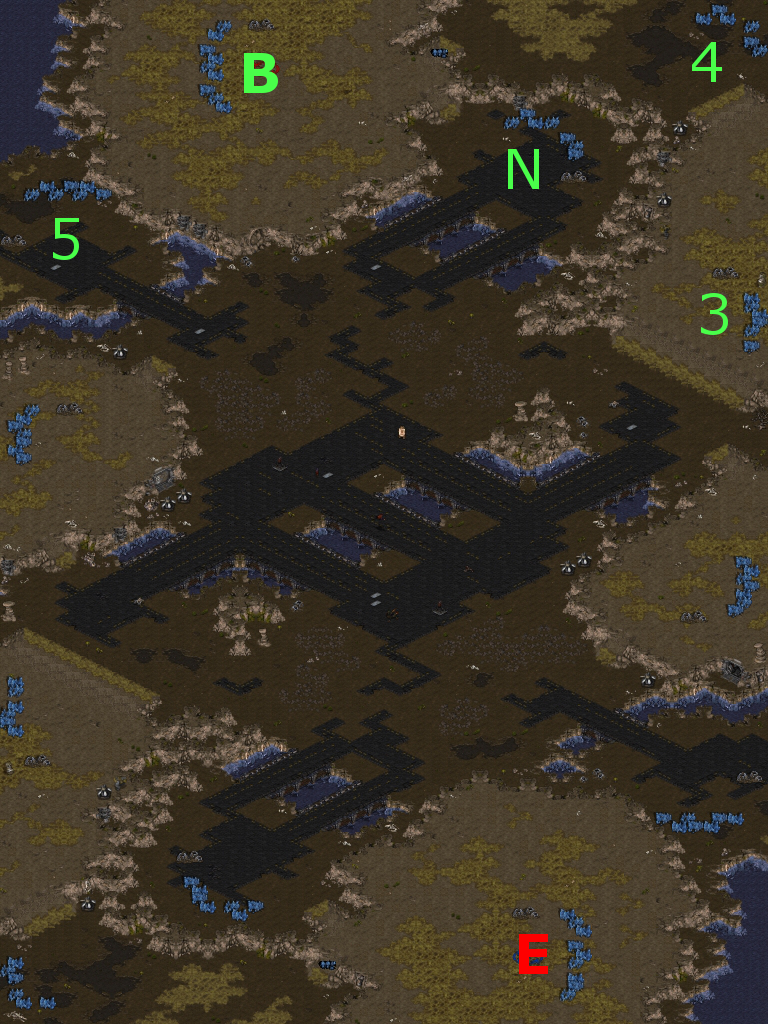
\includegraphics[scale=0.2]{Imagens/exp-dest-top.jpg}
	\caption[Ordem de expans�o visto em partida profissional no mapa Destination.]{Ordem de expans�o visto em partida profissional no mapa Destination. B indica a posi��o inicial, N indica a natural e os n�meros indicam as expans�es al�m da natural, na ordem que ser�o tomadas.}
	\label{fig:exp-dest}
\end{figure}

A ordem vista no mapa Destination (Figura~\ref{fig:exp-dest}) foi seguida fielmente pelo Cerebrate. O mesmo n�o pode ser dito do que ocorreu nos outros mapas, onde a l�gica por tr�s da ordem de expans�o n�o � a mesma.

No mapa Fighting Spirit, as expans�es tendem a ser em outras posi��es iniciais, como pode visto na Figura~\ref{fig:exp-fight}. Isto se deve ao fato de a ra�a Zerg possuir a estrutura \emph{Nydus Canal} (Figura~\ref{fig:nyduslurker}.a). Esta estrutura permite o transporte instant�neo de unidades de um extremo a outro do canal. Isso permite ao jogador defender em pouco tempo uma base que esteja longe de sua principal. O modelo proposto n�o leva em considera��o a possibilidade de usar essa estrutura, de forma que a ordem escolhida foi com as bases mais pr�ximas. Outro ponto importante na escolha das expans�es, para o jogador humano, � a facilidade de defender um ataque terrestre. Uma vez que as bases possuem apenas um gargalo que as ligam com o resto do mapa, � poss�vel utilizar as unidades \emph{lurkers}\footnote{Unidade zerg que causa dano em �rea com seus ataques. Precisa enterrar-se para atacar, torndando-se uma unidade invis�vel no processo.} (Figura~\ref{fig:nyduslurker}.b) para defender o gargalo. Esta configura��o de principal, com apenas um gargalo longe da localiza��o da base, se mostra mais f�cil de defender que bases com v�rios gargalos e com uma �rea pequena.

\begin{figure}[H]
	\centering
	\subfloat[Ordem feita por um jogador profissional (Canto superior esquerdo)]{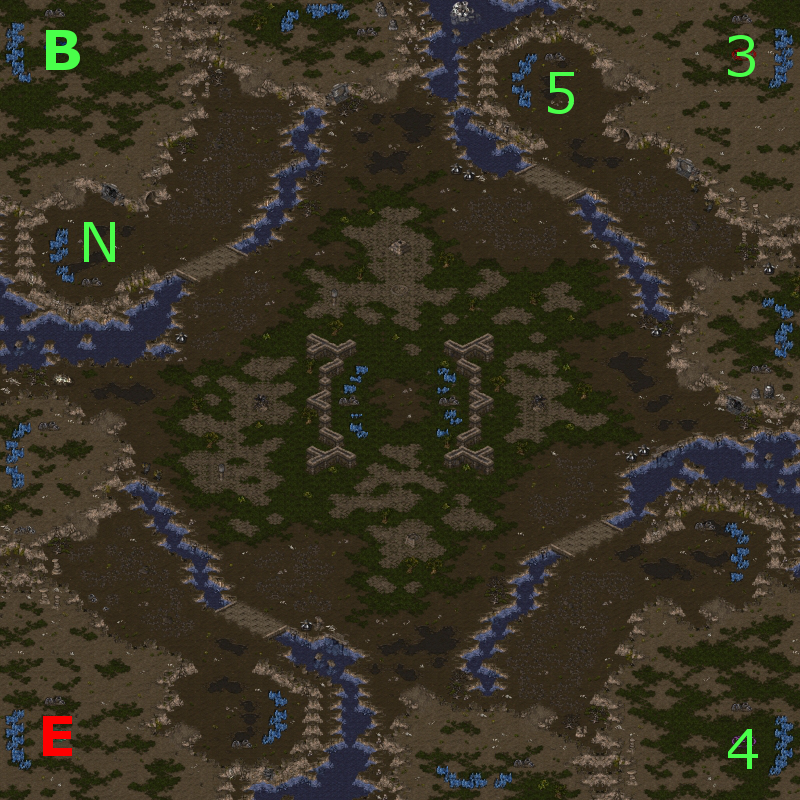
\includegraphics[scale=0.2]{Imagens/exp-fight-topl.jpg}}
	\qquad
	\subfloat[Ordem feita pelo Cerebrate (Canto superior esquerdo)]{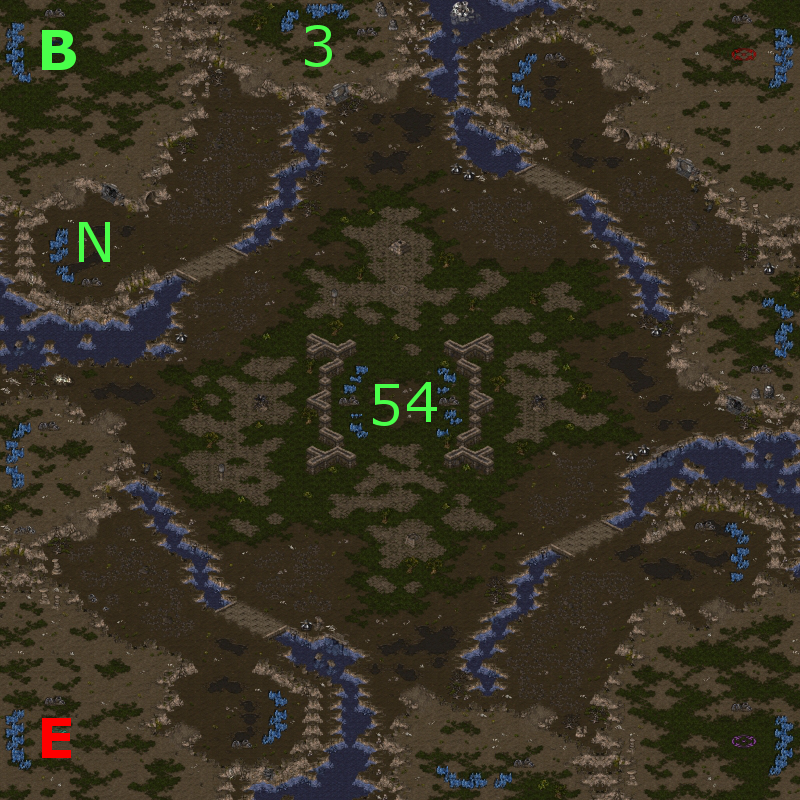
\includegraphics[scale=0.2]{Imagens/exp-fight-topl--.jpg}}
	\qquad
	\subfloat[Ordem feita por um jogador profissional (Canto inferior direito)]{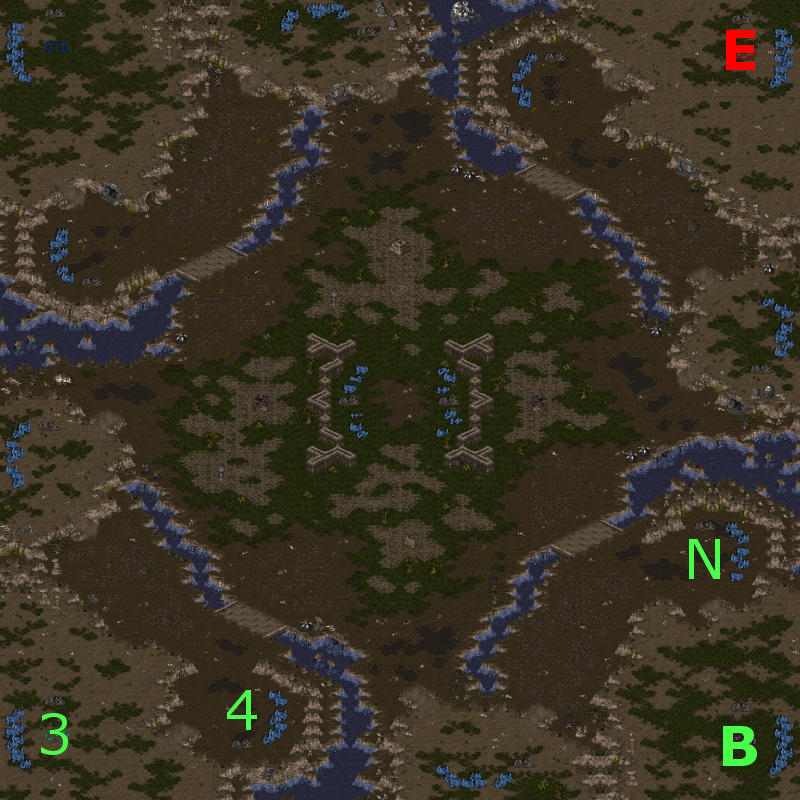
\includegraphics[scale=0.2]{Imagens/exp-fight-botr.jpg}}
	\qquad
	\subfloat[Ordem feita pelo Cerebrate (Canto inferior direito)]{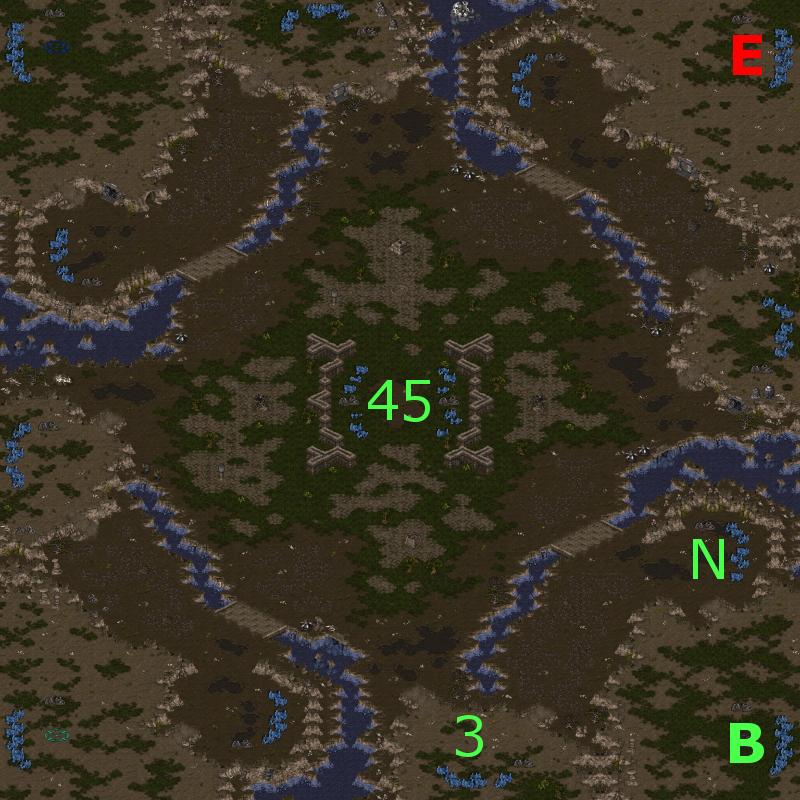
\includegraphics[scale=0.2]{Imagens/exp-fight-botr--.jpg}}
	\caption[Compara��o de ordens de expans�o no mapa Fighting Spirit.]{Compara��o de ordens de expans�o no mapa Fighting Spirit. B indica a posi��o inicial, N indica a natural e os n�meros indicam as expans�es al�m da natural, na ordem que ser�o tomadas.}
	\label{fig:exp-fight}
\end{figure}

\begin{figure}[H]
	\centering
	\subfloat[Nydus Canal]{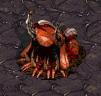
\includegraphics{Imagens/Nydus_canal.jpg}}
	\qquad
	\subfloat[Lurker]{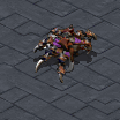
\includegraphics[scale=0.8]{Imagens/Lurker.png}}
	\caption{Elementos desconsiderados na cria��o da fun��o de avalia��o de bases.}
	\label{fig:nyduslurker}
\end{figure}

\section{Posicionamento de Estruturas}
A Tabela~\ref{tab:buildpos} mostra a soma de todas as brechas das muralhas em pixels. Como o objetivo deste sistema � a minimiza��o desta soma, quanto maior o n�mero, pior o posicionamento das estruturas. Pelos resultados mostrados nesta tabela, as muralhas propostas pelo Cerebrate ficam aqu�m das recomenda��es de jogadores experientes de StarCraft. Apenas em um caso, o Cerebrate conseguiu atingir a expectativa, na posi��o superior do mapa Destination.

\begin{table}[h]
	% T�tulo de tabelas sempre aparecem antes da tabela
	\center
	{
		\begin{tabular}{l|l|l}
			\hline
			\textbf{Caso} & \textbf{Brechas} & \textbf{Brechas}\\
				& \textbf{(Cerebrate)} & \textbf{(TeamLiquid.net)}\\
			\hline
			Destination (superior) & 75 & 75\\
			Destination (inferior) & 97 & 82\\
			Fighting Spirit (superior direita) & 75 & 51\\
			Fighting Spirit (superior esquerda) & 61 & 49\\
			Fighting Spirit (inferior direita) & 62 & 52\\
			Fighting Spirit (inferior esquerda) & 76 & 61\\
			\hline
		\end{tabular}
	}
	\caption{Brechas dos modelos de muralha propostos pelo Cerebrate e pelo site TeamLiquid.}
	\label{tab:buildpos}
\end{table}

\begin{figure}[H]
	\centering
	\subfloat[TeamLiquid (Posi��o superior)]{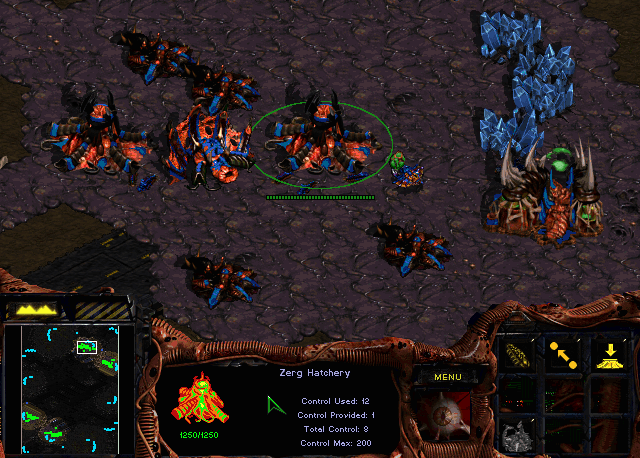
\includegraphics[scale=0.28]{Imagens/ZwDestination12-.png}}
	\qquad
	\subfloat[Cerebrate (Posi��o superior)]{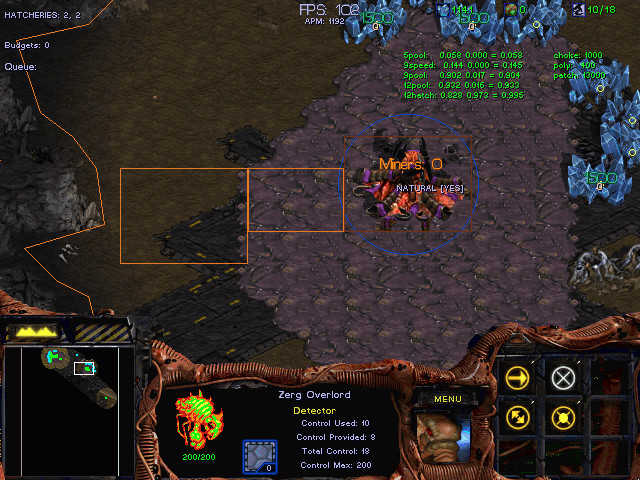
\includegraphics[scale=0.28]{Imagens/Dest-top.jpg}}
	\qquad
	\subfloat[TeamLiquid (Posi��o inferior)]{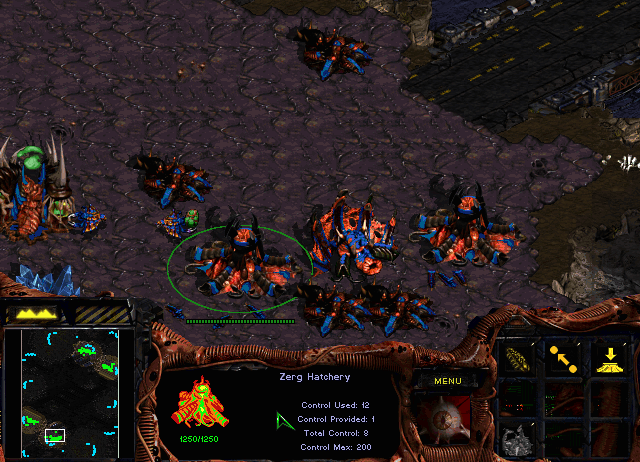
\includegraphics[scale=0.28]{Imagens/ZwDestination6.png}}
	\qquad
	\subfloat[Cerebrate (Posi��o inferior)]{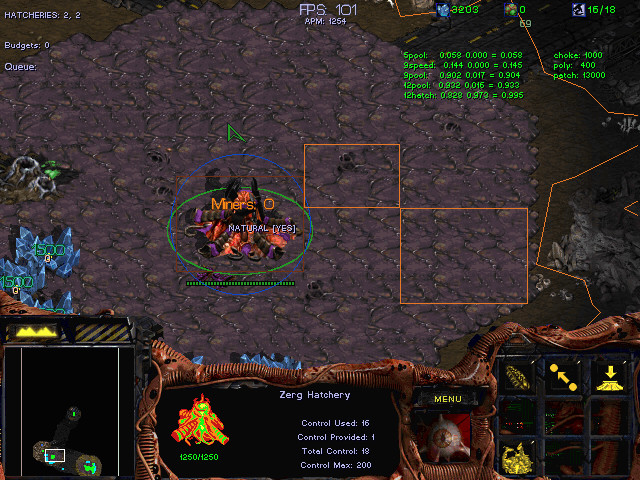
\includegraphics[scale=0.28]{Imagens/Dest-bot.jpg}}
	\caption{Compara��o de muralhas no mapa Destination.}
	\label{fig:wall-dest}
\end{figure}

\begin{figure}[H]
	\centering
	\subfloat[TeamLiquid (Canto inferior direito)]{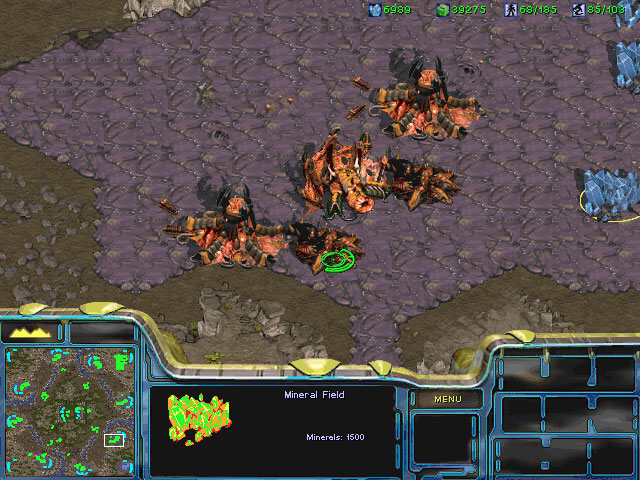
\includegraphics[scale=0.28]{Imagens/FS4Zerg.jpg}}
	\qquad
	\subfloat[Cerebrate (Canto inferior direito)]{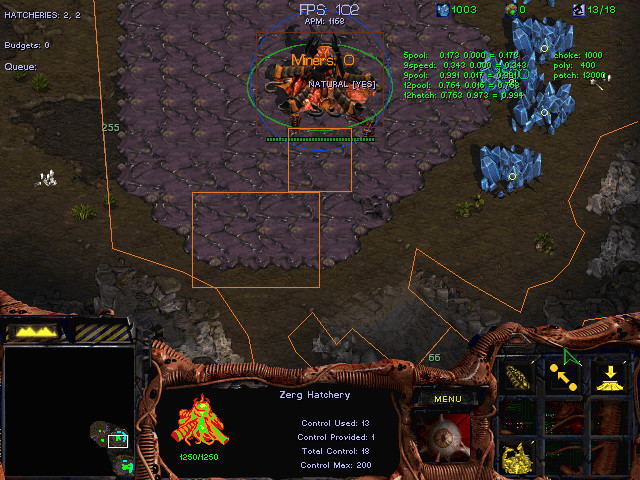
\includegraphics[scale=0.28]{Imagens/Figh-botr.jpg}}
	\qquad
	\subfloat[TeamLiquid (Canto inferior esquerdo)]{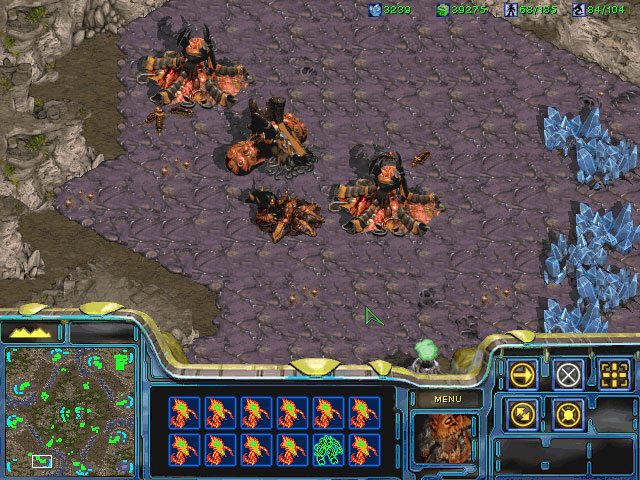
\includegraphics[scale=0.28]{Imagens/FS7Zerg.jpg}}
	\qquad
	\subfloat[Cerebrate (Canto inferior esquerdo)]{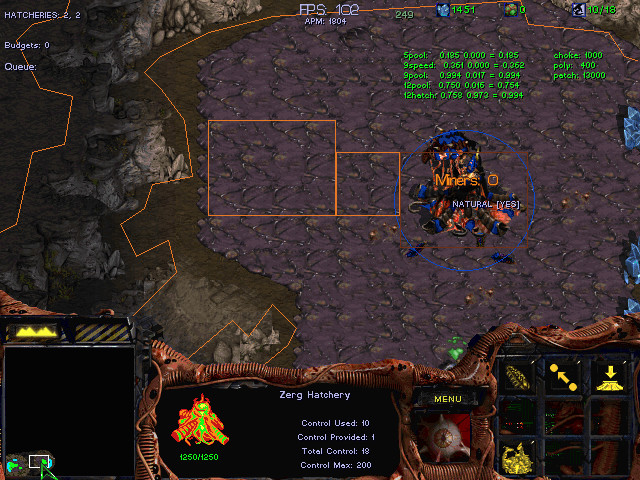
\includegraphics[scale=0.28]{Imagens/Figh-botl.jpg}}
	\qquad
	\subfloat[TeamLiquid (Canto superior direito)]{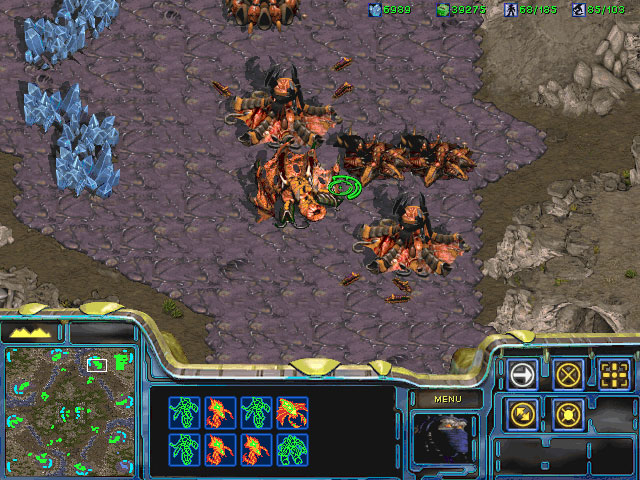
\includegraphics[scale=0.28]{Imagens/FS1Zerg.jpg}}
	\qquad
	\subfloat[Cerebrate (Canto superior direito)]{\includegraphics[scale=0.28]{Imagens/Figh-topr.jpg}}
	\qquad
	\subfloat[TeamLiquid (Canto superior esquerdo)]{\includegraphics[scale=0.28]{Imagens/FS10Zerg.jpg}}
	\qquad
	\subfloat[Cerebrate (Canto superior esquerdo)]{\includegraphics[scale=0.28]{Imagens/Figh-topl.jpg}}
	\caption{Compara��o de muralhas nas posi��es iniciais de Fighting Spirit.}
	\label{fig:wall-fight}
\end{figure}

As muralhas alocadas em Destination (Figura~\ref{fig:wall-dest}) ficaram muito pr�ximas das recomenda��es, com uma das constru��es mais � frente ou atr�s do que deveria ser. A diferen�a do resultado da posi��o inferior se d� porque n�o h� uma compara��o de quantos blocos est�o tocando a aloca��o anterior. J� a diferen�a do resultado da posi��o superior se d� pelo fato de que todos os blocos est�o mais pr�ximos do per�metro da regi�o na sugest�o do Cerebrate do que na posi��o sugerida pelo f�rum.

A figura \ref{fig:wall-fight} mostra a compara��o entre as muralhas do mapa Fighting Spirit. Destas imagens duas informa��es importantes podem ser tiradas. A primeira � que o algoritmo n�o leva em considera��o a quantidade de blocos de movimenta��o que existem em um bloco de constru��o. Desta forma, a muralha acaba por ser atra�da blocos de constru��o que possibilitam a passagem de unidades, como � poss�vel observar na Figura~\ref{fig:wall-fight}.d e na Figura~\ref{fig:wall-fight}.f.

A segunda informa��o importante � a dist�ncia que existe entre as muralhas e os gargalos. As muralhas propostas possuem uma dist�ncia muito pequena para o maior gargalo, procurando deixar a muralha com a menor brecha poss�vel. J� as muralhas alocadas pelo Cerebrate possuem uma dist�ncia grande, pois o valor da carga repulsiva � proporcional � largura do gargalo.

\section{Aberturas}
%attack frame: 4545

\begin{figure}[H]
	\begin{tikzpicture}
		\begin{axis}[
			width=15cm,height=7cm,
			xlabel={\footnotesize{Quadros}},
			ylabel={\footnotesize{Min�rios coletados}},
			legend style={at={(0,0.25)},anchor=south west},
			xmin=1, ymin = 0,ymax=1800]

			\addplot[color={sixpool}] coordinates {

				(1,0) (2,0) (3,0) (4,0) (5,0) (6,0) (7,0) (8,0) (9,0) (10,0) (11,0) (12,0) (13,0) (14,0) (15,0) (16,0) (17,0) (18,0) (19,0) (20,0) (21,0) (22,0) (23,0) (24,0) (25,0) (26,0) (27,0) (28,0) (29,0) (30,0) (31,0) (32,0) (33,0) (34,0) (35,0) (36,0) (37,0) (38,0) (39,0) (40,0) (41,0) (42,0) (43,0) (44,0) (45,0) (46,0) (47,0) (48,0) (49,0) (50,0) (51,0) (52,0) (53,0) (54,0) (55,0) (56,0) (57,0) (58,0) (59,0) (60,0) (61,0) (62,0) (63,0) (64,0) (65,0) (66,0) (67,0) (68,0) (69,0) (70,0) (71,0) (72,0) (73,0) (74,0) (75,0) (76,0) (77,0) (78,0) (79,0) (80,0) (81,0) (82,0) (83,0) (84,0) (85,0) (86,0) (87,0) (88,0) (89,0) (90,0) (91,0) (92,0) (93,0) (94,0) (95,0) (96,0) (97,0) (98,0) (99,0) (100,0) (101,0) (102,0) (103,0) (104,0) (105,0) (106,0) (107,0) (108,0) (109,0) (110,0) (111,0) (112,0) (113,0) (114,0) (115,0) (116,0) (117,0) (118,0) (119,0) (120,0) (121,0) (122,0) (123,0) (124,0) (125,0) (126,0) (127,0) (128,0) (129,0) (130,0) (131,0) (132,0) (133,0) (134,0) (135,0) (136,0) (137,0) (138,0) (139,0) (140,0) (141,0) (142,0) (143,0) (144,0) (145,0) (146,0) (147,0) (148,0) (149,0) (150,0) (151,0) (152,0) (153,0) (154,0) (155,0) (156,8) (157,8) (158,8) (159,8) (160,8) (161,8) (162,8) (163,8) (164,8) (165,8) (166,8) (167,8) (168,8) (169,8) (170,8) (171,8) (172,8) (173,8) (174,8) (175,8) (176,16) (177,24) (178,24) (179,24) (180,24) (181,24) (182,24) (183,24) (184,24) (185,24) (186,24) (187,24) (188,24) (189,24) (190,24) (191,24) (192,24) (193,24) (194,24) (195,24) (196,24) (197,24) (198,24) (199,24) (200,24) (201,24) (202,24) (203,24) (204,24) (205,24) (206,32) (207,32) (208,32) (209,32) (210,32) (211,32) (212,32) (213,32) (214,32) (215,32) (216,32) (217,32) (218,32) (219,32) (220,32) (221,32) (222,32) (223,32) (224,32) (225,32) (226,32) (227,32) (228,32) (229,32) (230,32) (231,32) (232,32) (233,32) (234,32) (235,32) (236,32) (237,32) (238,32) (239,32) (240,32) (241,32) (242,32) (243,32) (244,32) (245,32) (246,32) (247,32) (248,32) (249,32) (250,32) (251,32) (252,32) (253,32) (254,32) (255,32) (256,32) (257,32) (258,32) (259,32) (260,32) (261,32) (262,32) (263,32) (264,32) (265,32) (266,32) (267,32) (268,32) (269,32) (270,32) (271,32) (272,32) (273,32) (274,32) (275,32) (276,32) (277,32) (278,32) (279,32) (280,32) (281,32) (282,32) (283,32) (284,32) (285,32) (286,32) (287,32) (288,32) (289,32) (290,32) (291,32) (292,32) (293,32) (294,32) (295,32) (296,32) (297,32) (298,32) (299,32) (300,32) (301,32) (302,32) (303,32) (304,32) (305,32) (306,32) (307,32) (308,32) (309,32) (310,32) (311,32) (312,32) (313,32) (314,32) (315,32) (316,32) (317,32) (318,32) (319,32) (320,32) (321,32) (322,32) (323,32) (324,40) (325,40) (326,40) (327,40) (328,40) (329,40) (330,40) (331,40) (332,40) (333,40) (334,40) (335,48) (336,48) (337,48) (338,48) (339,48) (340,48) (341,48) (342,48) (343,48) (344,48) (345,48) (346,56) (347,56) (348,56) (349,56) (350,56) (351,56) (352,56) (353,56) (354,56) (355,56) (356,56) (357,56) (358,56) (359,56) (360,56) (361,56) (362,56) (363,56) (364,56) (365,56) (366,56) (367,56) (368,56) (369,56) (370,56) (371,56) (372,56) (373,56) (374,56) (375,56) (376,56) (377,56) (378,56) (379,56) (380,56) (381,56) (382,56) (383,64) (384,64) (385,64) (386,64) (387,64) (388,64) (389,64) (390,64) (391,64) (392,64) (393,64) (394,64) (395,64) (396,64) (397,64) (398,64) (399,64) (400,64) (401,64) (402,64) (403,64) (404,64) (405,64) (406,64) (407,64) (408,64) (409,64) (410,64) (411,64) (412,64) (413,64) (414,64) (415,64) (416,64) (417,64) (418,64) (419,64) (420,64) (421,64) (422,64) (423,64) (424,64) (425,64) (426,64) (427,64) (428,64) (429,64) (430,64) (431,64) (432,64) (433,64) (434,64) (435,64) (436,64) (437,64) (438,64) (439,64) (440,64) (441,64) (442,64) (443,64) (444,64) (445,64) (446,64) (447,64) (448,64) (449,64) (450,64) (451,64) (452,64) (453,64) (454,64) (455,64) (456,64) (457,64) (458,64) (459,64) (460,64) (461,64) (462,64) (463,64) (464,64) (465,64) (466,64) (467,64) (468,64) (469,64) (470,64) (471,64) (472,64) (473,64) (474,64) (475,64) (476,64) (477,64) (478,64) (479,64) (480,64) (481,64) (482,64) (483,64) (484,64) (485,64) (486,64) (487,64) (488,64) (489,64) (490,64) (491,64) (492,64) (493,64) (494,72) (495,72) (496,80) (497,80) (498,80) (499,80) (500,80) (501,80) (502,80) (503,80) (504,80) (505,80) (506,80) (507,80) (508,80) (509,80) (510,80) (511,80) (512,80) (513,80) (514,80) (515,88) (516,88) (517,88) (518,88) (519,88) (520,88) (521,88) (522,88) (523,88) (524,88) (525,88) (526,88) (527,88) (528,88) (529,88) (530,88) (531,88) (532,88) (533,88) (534,88) (535,88) (536,88) (537,88) (538,88) (539,88) (540,88) (541,88) (542,88) (543,88) (544,88) (545,88) (546,88) (547,88) (548,88) (549,88) (550,88) (551,88) (552,88) (553,88) (554,88) (555,88) (556,88) (557,88) (558,88) (559,88) (560,88) (561,96) (562,96) (563,96) (564,96) (565,96) (566,96) (567,96) (568,96) (569,96) (570,96) (571,96) (572,96) (573,96) (574,96) (575,96) (576,96) (577,96) (578,96) (579,96) (580,96) (581,96) (582,96) (583,96) (584,96) (585,96) (586,96) (587,96) (588,96) (589,96) (590,96) (591,96) (592,96) (593,96) (594,96) (595,96) (596,96) (597,96) (598,96) (599,96) (600,96) (601,96) (602,96) (603,96) (604,96) (605,96) (606,96) (607,96) (608,96) (609,96) (610,96) (611,96) (612,96) (613,96) (614,96) (615,96) (616,96) (617,96) (618,96) (619,96) (620,96) (621,104) (622,104) (623,104) (624,104) (625,104) (626,104) (627,104) (628,104) (629,104) (630,104) (631,104) (632,104) (633,104) (634,104) (635,104) (636,104) (637,104) (638,104) (639,104) (640,104) (641,104) (642,104) (643,104) (644,104) (645,104) (646,104) (647,104) (648,104) (649,104) (650,104) (651,104) (652,104) (653,104) (654,104) (655,104) (656,104) (657,112) (658,112) (659,112) (660,112) (661,112) (662,112) (663,112) (664,112) (665,120) (666,120) (667,120) (668,120) (669,120) (670,120) (671,120) (672,120) (673,120) (674,120) (675,120) (676,120) (677,120) (678,120) (679,120) (680,120) (681,120) (682,120) (683,120) (684,120) (685,128) (686,128) (687,128) (688,128) (689,128) (690,128) (691,128) (692,128) (693,128) (694,128) (695,128) (696,128) (697,128) (698,128) (699,128) (700,128) (701,128) (702,128) (703,128) (704,128) (705,128) (706,128) (707,128) (708,128) (709,128) (710,128) (711,128) (712,128) (713,128) (714,128) (715,128) (716,128) (717,128) (718,128) (719,128) (720,128) (721,128) (722,128) (723,128) (724,128) (725,128) (726,128) (727,128) (728,128) (729,128) (730,128) (731,128) (732,128) (733,128) (734,128) (735,128) (736,128) (737,128) (738,128) (739,128) (740,128) (741,128) (742,136) (743,136) (744,136) (745,136) (746,136) (747,136) (748,136) (749,136) (750,136) (751,136) (752,136) (753,136) (754,136) (755,136) (756,136) (757,136) (758,136) (759,136) (760,136) (761,136) (762,136) (763,136) (764,136) (765,136) (766,136) (767,136) (768,136) (769,136) (770,136) (771,136) (772,136) (773,136) (774,136) (775,136) (776,136) (777,136) (778,136) (779,136) (780,136) (781,136) (782,136) (783,136) (784,136) (785,136) (786,136) (787,136) (788,136) (789,136) (790,136) (791,136) (792,136) (793,136) (794,136) (795,136) (796,136) (797,136) (798,136) (799,144) (800,144) (801,144) (802,144) (803,144) (804,144) (805,144) (806,144) (807,144) (808,144) (809,144) (810,144) (811,144) (812,144) (813,144) (814,144) (815,144) (816,144) (817,152) (818,152) (819,152) (820,152) (821,152) (822,152) (823,152) (824,152) (825,152) (826,152) (827,152) (828,152) (829,152) (830,152) (831,152) (832,152) (833,152) (834,160) (835,160) (836,160) (837,160) (838,160) (839,160) (840,160) (841,160) (842,160) (843,160) (844,160) (845,160) (846,160) (847,160) (848,160) (849,160) (850,160) (851,160) (852,160) (853,160) (854,168) (855,168) (856,168) (857,168) (858,168) (859,168) (860,168) (861,168) (862,168) (863,168) (864,168) (865,168) (866,168) (867,168) (868,168) (869,168) (870,168) (871,168) (872,168) (873,168) (874,168) (875,168) (876,168) (877,168) (878,168) (879,168) (880,168) (881,168) (882,168) (883,168) (884,168) (885,168) (886,168) (887,168) (888,168) (889,168) (890,168) (891,168) (892,168) (893,168) (894,168) (895,168) (896,168) (897,168) (898,168) (899,168) (900,168) (901,168) (902,168) (903,168) (904,168) (905,168) (906,168) (907,168) (908,168) (909,168) (910,168) (911,168) (912,168) (913,168) (914,168) (915,168) (916,168) (917,168) (918,168) (919,168) (920,168) (921,168) (922,168) (923,168) (924,176) (925,176) (926,176) (927,176) (928,176) (929,176) (930,176) (931,176) (932,176) (933,176) (934,176) (935,176) (936,176) (937,176) (938,176) (939,176) (940,176) (941,176) (942,176) (943,176) (944,176) (945,176) (946,176) (947,176) (948,176) (949,176) (950,176) (951,176) (952,176) (953,176) (954,176) (955,176) (956,176) (957,176) (958,176) (959,176) (960,176) (961,176) (962,176) (963,176) (964,176) (965,176) (966,176) (967,176) (968,176) (969,184) (970,184) (971,184) (972,184) (973,184) (974,184) (975,184) (976,184) (977,192) (978,192) (979,192) (980,192) (981,192) (982,192) (983,192) (984,192) (985,192) (986,192) (987,192) (988,192) (989,192) (990,192) (991,192) (992,192) (993,192) (994,192) (995,192) (996,192) (997,192) (998,192) (999,192) (1000,192) (1001,192) (1002,192) (1003,200) (1004,200) (1005,200) (1006,200) (1007,200) (1008,200) (1009,200) (1010,200) (1011,200) (1012,200) (1013,200) (1014,200) (1015,200) (1016,200) (1017,200) (1018,200) (1019,200) (1020,200) (1021,200) (1022,200) (1023,208) (1024,208) (1025,208) (1026,208) (1027,208) (1028,208) (1029,208) (1030,208) (1031,208) (1032,208) (1033,208) (1034,208) (1035,208) (1036,208) (1037,208) (1038,208) (1039,208) (1040,208) (1041,208) (1042,208) (1043,208) (1044,208) (1045,208) (1046,208) (1047,208) (1048,208) (1049,208) (1050,208) (1051,208) (1052,208) (1053,208) (1054,208) (1055,208) (1056,208) (1057,208) (1058,208) (1059,208) (1060,208) (1061,208) (1062,208) (1063,208) (1064,208) (1065,208) (1066,208) (1067,208) (1068,208) (1069,208) (1070,208) (1071,208) (1072,208) (1073,208) (1074,208) (1075,208) (1076,208) (1077,208) (1078,208) (1079,208) (1080,208) (1081,208) (1082,208) (1083,208) (1084,208) (1085,208) (1086,208) (1087,208) (1088,208) (1089,208) (1090,208) (1091,208) (1092,208) (1093,208) (1094,208) (1095,208) (1096,208) (1097,208) (1098,208) (1099,208) (1100,208) (1101,208) (1102,208) (1103,216) (1104,216) (1105,216) (1106,216) (1107,216) (1108,216) (1109,216) (1110,216) (1111,216) (1112,216) (1113,216) (1114,216) (1115,216) (1116,216) (1117,216) (1118,216) (1119,216) (1120,216) (1121,216) (1122,216) (1123,216) (1124,216) (1125,216) (1126,216) (1127,216) (1128,216) (1129,216) (1130,216) (1131,216) (1132,216) (1133,216) (1134,216) (1135,216) (1136,216) (1137,224) (1138,224) (1139,224) (1140,224) (1141,224) (1142,224) (1143,224) (1144,224) (1145,224) (1146,224) (1147,232) (1148,232) (1149,232) (1150,232) (1151,232) (1152,232) (1153,232) (1154,232) (1155,232) (1156,232) (1157,232) (1158,232) (1159,232) (1160,232) (1161,232) (1162,232) (1163,232) (1164,232) (1165,232) (1166,232) (1167,232) (1168,232) (1169,232) (1170,232) (1171,232) (1172,232) (1173,232) (1174,232) (1175,232) (1176,232) (1177,232) (1178,232) (1179,232) (1180,232) (1181,232) (1182,232) (1183,232) (1184,232) (1185,232) (1186,232) (1187,232) (1188,232) (1189,232) (1190,232) (1191,232) (1192,232) (1193,232) (1194,240) (1195,240) (1196,240) (1197,240) (1198,240) (1199,240) (1200,240) (1201,240) (1202,240) (1203,240) (1204,240) (1205,240) (1206,240) (1207,240) (1208,240) (1209,240) (1210,240) (1211,240) (1212,240) (1213,240) (1214,240) (1215,240) (1216,240) (1217,240) (1218,240) (1219,240) (1220,240) (1221,240) (1222,240) (1223,240) (1224,240) (1225,240) (1226,240) (1227,240) (1228,240) (1229,240) (1230,240) (1231,240) (1232,240) (1233,240) (1234,240) (1235,240) (1236,240) (1237,240) (1238,240) (1239,240) (1240,240) (1241,240) (1242,240) (1243,240) (1244,240) (1245,240) (1246,240) (1247,240) (1248,240) (1249,240) (1250,240) (1251,240) (1252,240) (1253,240) (1254,240) (1255,240) (1256,240) (1257,240) (1258,240) (1259,240) (1260,240) (1261,240) (1262,240) (1263,240) (1264,240) (1265,240) (1266,240) (1267,240) (1268,240) (1269,240) (1270,240) (1271,240) (1272,240) (1273,240) (1274,240) (1275,240) (1276,240) (1277,240) (1278,240) (1279,240) (1280,240) (1281,240) (1282,248) (1283,248) (1284,248) (1285,248) (1286,248) (1287,248) (1288,248) (1289,248) (1290,248) (1291,248) (1292,248) (1293,248) (1294,248) (1295,248) (1296,248) (1297,256) (1298,256) (1299,256) (1300,256) (1301,256) (1302,256) (1303,256) (1304,256) (1305,256) (1306,256) (1307,256) (1308,256) (1309,256) (1310,256) (1311,256) (1312,256) (1313,256) (1314,256) (1315,256) (1316,256) (1317,256) (1318,256) (1319,256) (1320,256) (1321,256) (1322,256) (1323,256) (1324,256) (1325,256) (1326,264) (1327,264) (1328,264) (1329,264) (1330,264) (1331,264) (1332,264) (1333,264) (1334,264) (1335,264) (1336,264) (1337,264) (1338,264) (1339,264) (1340,264) (1341,264) (1342,264) (1343,264) (1344,264) (1345,264) (1346,264) (1347,264) (1348,264) (1349,264) (1350,264) (1351,264) (1352,264) (1353,264) (1354,264) (1355,264) (1356,264) (1357,264) (1358,264) (1359,264) (1360,264) (1361,264) (1362,264) (1363,264) (1364,264) (1365,264) (1366,264) (1367,272) (1368,272) (1369,272) (1370,272) (1371,272) (1372,272) (1373,272) (1374,272) (1375,272) (1376,272) (1377,272) (1378,272) (1379,272) (1380,272) (1381,272) (1382,272) (1383,272) (1384,272) (1385,272) (1386,272) (1387,272) (1388,272) (1389,272) (1390,272) (1391,272) (1392,272) (1393,272) (1394,272) (1395,272) (1396,272) (1397,272) (1398,272) (1399,272) (1400,272) (1401,272) (1402,272) (1403,272) (1404,272) (1405,272) (1406,272) (1407,272) (1408,272) (1409,272) (1410,272) (1411,272) (1412,272) (1413,272) (1414,272) (1415,272) (1416,272) (1417,272) (1418,272) (1419,272) (1420,272) (1421,272) (1422,272) (1423,272) (1424,272) (1425,272) (1426,272) (1427,272) (1428,272) (1429,272) (1430,272) (1431,272) (1432,272) (1433,272) (1434,272) (1435,272) (1436,272) (1437,272) (1438,272) (1439,272) (1440,272) (1441,272) (1442,272) (1443,272) (1444,272) (1445,272) (1446,272) (1447,272) (1448,272) (1449,272) (1450,272) (1451,272) (1452,272) (1453,272) (1454,272) (1455,272) (1456,280) (1457,280) (1458,280) (1459,288) (1460,288) (1461,288) (1462,288) (1463,288) (1464,288) (1465,288) (1466,288) (1467,288) (1468,288) (1469,288) (1470,288) (1471,288) (1472,288) (1473,288) (1474,288) (1475,288) (1476,288) (1477,288) (1478,288) (1479,288) (1480,288) (1481,288) (1482,288) (1483,288) (1484,288) (1485,288) (1486,288) (1487,288) (1488,288) (1489,288) (1490,288) (1491,288) (1492,288) (1493,288) (1494,288) (1495,288) (1496,288) (1497,288) (1498,288) (1499,288) (1500,288) (1501,288) (1502,288) (1503,288) (1504,288) (1505,296) (1506,296) (1507,296) (1508,296) (1509,296) (1510,296) (1511,296) (1512,296) (1513,296) (1514,296) (1515,296) (1516,296) (1517,296) (1518,296) (1519,296) (1520,296) (1521,296) (1522,296) (1523,296) (1524,296) (1525,296) (1526,296) (1527,296) (1528,296) (1529,296) (1530,296) (1531,296) (1532,296) (1533,296) (1534,296) (1535,296) (1536,304) (1537,304) (1538,304) (1539,304) (1540,304) (1541,304) (1542,304) (1543,304) (1544,304) (1545,304) (1546,304) (1547,304) (1548,304) (1549,304) (1550,304) (1551,304) (1552,304) (1553,304) (1554,304) (1555,304) (1556,304) (1557,304) (1558,304) (1559,304) (1560,304) (1561,304) (1562,304) (1563,304) (1564,304) (1565,304) (1566,304) (1567,304) (1568,304) (1569,304) (1570,304) (1571,304) (1572,304) (1573,304) (1574,304) (1575,304) (1576,304) (1577,304) (1578,304) (1579,304) (1580,304) (1581,304) (1582,304) (1583,304) (1584,304) (1585,304) (1586,304) (1587,304) (1588,304) (1589,304) (1590,304) (1591,304) (1592,304) (1593,304) (1594,304) (1595,304) (1596,304) (1597,304) (1598,304) (1599,304) (1600,304) (1601,304) (1602,304) (1603,304) (1604,304) (1605,304) (1606,304) (1607,304) (1608,304) (1609,304) (1610,304) (1611,304) (1612,304) (1613,304) (1614,304) (1615,304) (1616,304) (1617,312) (1618,312) (1619,312) (1620,312) (1621,312) (1622,312) (1623,312) (1624,312) (1625,312) (1626,312) (1627,312) (1628,312) (1629,312) (1630,312) (1631,312) (1632,312) (1633,312) (1634,312) (1635,312) (1636,312) (1637,312) (1638,312) (1639,320) (1640,320) (1641,320) (1642,320) (1643,320) (1644,320) (1645,320) (1646,320) (1647,320) (1648,320) (1649,320) (1650,320) (1651,320) (1652,320) (1653,320) (1654,320) (1655,320) (1656,320) (1657,320) (1658,320) (1659,320) (1660,320) (1661,320) (1662,320) (1663,320) (1664,320) (1665,320) (1666,320) (1667,320) (1668,320) (1669,320) (1670,320) (1671,320) (1672,320) (1673,320) (1674,320) (1675,320) (1676,320) (1677,320) (1678,320) (1679,320) (1680,320) (1681,320) (1682,320) (1683,320) (1684,320) (1685,320) (1686,320) (1687,328) (1688,328) (1689,328) (1690,328) (1691,328) (1692,328) (1693,328) (1694,328) (1695,328) (1696,328) (1697,328) (1698,328) (1699,328) (1700,328) (1701,328) (1702,328) (1703,328) (1704,328) (1705,328) (1706,336) (1707,336) (1708,336) (1709,336) (1710,336) (1711,336) (1712,336) (1713,336) (1714,336) (1715,336) (1716,336) (1717,336) (1718,336) (1719,336) (1720,336) (1721,336) (1722,336) (1723,336) (1724,336) (1725,336) (1726,336) (1727,336) (1728,336) (1729,336) (1730,336) (1731,336) (1732,336) (1733,336) (1734,336) (1735,336) (1736,336) (1737,336) (1738,336) (1739,336) (1740,336) (1741,336) (1742,336) (1743,336) (1744,336) (1745,336) (1746,336) (1747,336) (1748,336) (1749,336) (1750,336) (1751,336) (1752,336) (1753,336) (1754,336) (1755,336) (1756,336) (1757,336) (1758,336) (1759,336) (1760,336) (1761,336) (1762,336) (1763,336) (1764,336) (1765,336) (1766,336) (1767,336) (1768,336) (1769,336) (1770,336) (1771,336) (1772,336) (1773,336) (1774,336) (1775,336) (1776,336) (1777,336) (1778,336) (1779,344) (1780,344) (1781,344) (1782,344) (1783,344) (1784,344) (1785,344) (1786,344) (1787,344) (1788,344) (1789,344) (1790,344) (1791,344) (1792,344) (1793,344) (1794,344) (1795,344) (1796,344) (1797,344) (1798,344) (1799,344) (1800,344) (1801,344) (1802,344) (1803,344) (1804,344) (1805,344) (1806,344) (1807,344) (1808,344) (1809,344) (1810,344) (1811,344) (1812,344) (1813,344) (1814,344) (1815,344) (1816,344) (1817,344) (1818,344) (1819,344) (1820,352) (1821,352) (1822,352) (1823,352) (1824,352) (1825,352) (1826,352) (1827,352) (1828,352) (1829,352) (1830,352) (1831,352) (1832,352) (1833,352) (1834,352) (1835,352) (1836,352) (1837,352) (1838,352) (1839,352) (1840,352) (1841,352) (1842,352) (1843,352) (1844,352) (1845,352) (1846,352) (1847,352) (1848,352) (1849,352) (1850,352) (1851,352) (1852,352) (1853,352) (1854,352) (1855,352) (1856,352) (1857,352) (1858,352) (1859,352) (1860,352) (1861,352) (1862,352) (1863,352) (1864,360) (1865,368) (1866,368) (1867,368) (1868,368) (1869,368) (1870,368) (1871,368) (1872,368) (1873,368) (1874,376) (1875,376) (1876,376) (1877,376) (1878,376) (1879,376) (1880,376) (1881,376) (1882,376) (1883,376) (1884,376) (1885,376) (1886,376) (1887,376) (1888,376) (1889,376) (1890,376) (1891,376) (1892,376) (1893,376) (1894,376) (1895,376) (1896,376) (1897,376) (1898,376) (1899,376) (1900,376) (1901,376) (1902,376) (1903,376) (1904,376) (1905,376) (1906,376) (1907,376) (1908,376) (1909,376) (1910,376) (1911,376) (1912,376) (1913,376) (1914,376) (1915,376) (1916,376) (1917,376) (1918,376) (1919,376) (1920,376) (1921,376) (1922,376) (1923,376) (1924,376) (1925,376) (1926,376) (1927,376) (1928,376) (1929,376) (1930,376) (1931,376) (1932,376) (1933,376) (1934,376) (1935,376) (1936,376) (1937,376) (1938,376) (1939,376) (1940,376) (1941,376) (1942,376) (1943,376) (1944,376) (1945,376) (1946,376) (1947,384) (1948,384) (1949,384) (1950,384) (1951,384) (1952,384) (1953,384) (1954,384) (1955,384) (1956,384) (1957,384) (1958,384) (1959,384) (1960,384) (1961,384) (1962,384) (1963,384) (1964,384) (1965,384) (1966,384) (1967,384) (1968,384) (1969,384) (1970,384) (1971,384) (1972,384) (1973,384) (1974,384) (1975,384) (1976,384) (1977,384) (1978,384) (1979,384) (1980,384) (1981,384) (1982,384) (1983,384) (1984,384) (1985,384) (1986,384) (1987,384) (1988,384) (1989,384) (1990,384) (1991,384) (1992,384) (1993,384) (1994,384) (1995,384) (1996,384) (1997,392) (1998,392) (1999,392) (2000,392) (2001,392) (2002,392) (2003,392) (2004,392) (2005,392) (2006,392) (2007,392) (2008,392) (2009,392) (2010,392) (2011,392) (2012,392) (2013,392) (2014,392) (2015,392) (2016,392) (2017,392) (2018,392) (2019,392) (2020,392) (2021,392) (2022,392) (2023,392) (2024,392) (2025,392) (2026,392) (2027,392) (2028,392) (2029,392) (2030,392) (2031,392) (2032,400) (2033,400) (2034,400) (2035,400) (2036,400) (2037,400) (2038,400) (2039,400) (2040,400) (2041,400) (2042,416) (2043,416) (2044,416) (2045,416) (2046,416) (2047,416) (2048,416) (2049,416) (2050,416) (2051,416) (2052,416) (2053,416) (2054,416) (2055,416) (2056,416) (2057,416) (2058,416) (2059,416) (2060,416) (2061,416) (2062,416) (2063,416) (2064,416) (2065,416) (2066,416) (2067,416) (2068,416) (2069,416) (2070,416) (2071,416) (2072,416) (2073,416) (2074,416) (2075,416) (2076,416) (2077,416) (2078,416) (2079,416) (2080,416) (2081,416) (2082,416) (2083,416) (2084,416) (2085,416) (2086,416) (2087,416) (2088,416) (2089,416) (2090,416) (2091,416) (2092,416) (2093,416) (2094,416) (2095,416) (2096,416) (2097,416) (2098,416) (2099,416) (2100,416) (2101,416) (2102,416) (2103,416) (2104,416) (2105,416) (2106,416) (2107,416) (2108,416) (2109,416) (2110,424) (2111,424) (2112,424) (2113,424) (2114,432) (2115,432) (2116,432) (2117,432) (2118,432) (2119,432) (2120,432) (2121,432) (2122,432) (2123,432) (2124,432) (2125,432) (2126,432) (2127,432) (2128,432) (2129,432) (2130,432) (2131,432) (2132,432) (2133,432) (2134,432) (2135,432) (2136,432) (2137,432) (2138,432) (2139,432) (2140,432) (2141,432) (2142,432) (2143,432) (2144,432) (2145,432) (2146,432) (2147,432) (2148,432) (2149,432) (2150,432) (2151,432) (2152,432) (2153,432) (2154,432) (2155,432) (2156,432) (2157,432) (2158,432) (2159,432) (2160,432) (2161,432) (2162,432) (2163,432) (2164,432) (2165,432) (2166,432) (2167,440) (2168,440) (2169,440) (2170,440) (2171,440) (2172,440) (2173,440) (2174,440) (2175,440) (2176,440) (2177,440) (2178,440) (2179,440) (2180,440) (2181,440) (2182,440) (2183,440) (2184,440) (2185,440) (2186,440) (2187,440) (2188,440) (2189,440) (2190,440) (2191,440) (2192,440) (2193,440) (2194,440) (2195,440) (2196,440) (2197,440) (2198,440) (2199,440) (2200,440) (2201,448) (2202,448) (2203,448) (2204,448) (2205,448) (2206,448) (2207,448) (2208,448) (2209,448) (2210,448) (2211,456) (2212,456) (2213,456) (2214,456) (2215,456) (2216,456) (2217,456) (2218,456) (2219,456) (2220,464) (2221,464) (2222,464) (2223,464) (2224,464) (2225,464) (2226,464) (2227,464) (2228,464) (2229,464) (2230,464) (2231,464) (2232,464) (2233,464) (2234,464) (2235,464) (2236,464) (2237,464) (2238,464) (2239,464) (2240,464) (2241,464) (2242,464) (2243,464) (2244,464) (2245,464) (2246,464) (2247,464) (2248,464) (2249,464) (2250,464) (2251,464) (2252,464) (2253,464) (2254,464) (2255,464) (2256,464) (2257,464) (2258,464) (2259,464) (2260,464) (2261,464) (2262,464) (2263,464) (2264,464) (2265,464) (2266,464) (2267,464) (2268,464) (2269,464) (2270,472) (2271,472) (2272,472) (2273,472) (2274,472) (2275,472) (2276,472) (2277,472) (2278,472) (2279,472) (2280,472) (2281,472) (2282,472) (2283,472) (2284,472) (2285,472) (2286,472) (2287,472) (2288,472) (2289,472) (2290,472) (2291,472) (2292,472) (2293,472) (2294,472) (2295,472) (2296,472) (2297,472) (2298,472) (2299,472) (2300,472) (2301,480) (2302,480) (2303,480) (2304,480) (2305,480) (2306,480) (2307,480) (2308,480) (2309,480) (2310,480) (2311,480) (2312,480) (2313,480) (2314,480) (2315,480) (2316,480) (2317,480) (2318,480) (2319,480) (2320,480) (2321,480) (2322,480) (2323,480) (2324,480) (2325,480) (2326,480) (2327,480) (2328,480) (2329,480) (2330,480) (2331,480) (2332,480) (2333,480) (2334,480) (2335,480) (2336,480) (2337,480) (2338,480) (2339,480) (2340,480) (2341,480) (2342,480) (2343,480) (2344,480) (2345,488) (2346,488) (2347,488) (2348,488) (2349,488) (2350,488) (2351,488) (2352,488) (2353,488) (2354,488) (2355,488) (2356,488) (2357,488) (2358,488) (2359,488) (2360,488) (2361,488) (2362,488) (2363,488) (2364,488) (2365,488) (2366,488) (2367,488) (2368,488) (2369,488) (2370,496) (2371,496) (2372,496) (2373,496) (2374,496) (2375,496) (2376,496) (2377,496) (2378,496) (2379,496) (2380,496) (2381,496) (2382,504) (2383,504) (2384,504) (2385,504) (2386,504) (2387,504) (2388,504) (2389,504) (2390,504) (2391,504) (2392,504) (2393,504) (2394,504) (2395,504) (2396,504) (2397,504) (2398,504) (2399,504) (2400,512) (2401,512) (2402,512) (2403,512) (2404,512) (2405,512) (2406,512) (2407,512) (2408,512) (2409,512) (2410,512) (2411,512) (2412,512) (2413,512) (2414,512) (2415,512) (2416,512) (2417,512) (2418,512) (2419,512) (2420,512) (2421,512) (2422,512) (2423,512) (2424,512) (2425,512) (2426,512) (2427,512) (2428,512) (2429,520) (2430,520) (2431,520) (2432,520) (2433,520) (2434,520) (2435,520) (2436,520) (2437,520) (2438,520) (2439,520) (2440,520) (2441,520) (2442,520) (2443,520) (2444,520) (2445,520) (2446,520) (2447,520) (2448,520) (2449,520) (2450,520) (2451,520) (2452,520) (2453,520) (2454,520) (2455,520) (2456,520) (2457,520) (2458,520) (2459,520) (2460,520) (2461,520) (2462,520) (2463,520) (2464,520) (2465,520) (2466,520) (2467,520) (2468,520) (2469,520) (2470,520) (2471,520) (2472,520) (2473,520) (2474,520) (2475,520) (2476,520) (2477,520) (2478,520) (2479,520) (2480,520) (2481,520) (2482,520) (2483,520) (2484,520) (2485,520) (2486,520) (2487,520) (2488,528) (2489,528) (2490,528) (2491,528) (2492,528) (2493,528) (2494,528) (2495,528) (2496,528) (2497,528) (2498,528) (2499,528) (2500,528) (2501,528) (2502,528) (2503,528) (2504,528) (2505,528) (2506,528) (2507,528) (2508,528) (2509,528) (2510,528) (2511,528) (2512,528) (2513,528) (2514,528) (2515,528) (2516,528) (2517,528) (2518,528) (2519,528) (2520,528) (2521,528) (2522,536) (2523,536) (2524,536) (2525,536) (2526,536) (2527,536) (2528,536) (2529,536) (2530,536) (2531,536) (2532,536) (2533,536) (2534,536) (2535,536) (2536,536) (2537,536) (2538,536) (2539,536) (2540,544) (2541,544) (2542,544) (2543,544) (2544,544) (2545,544) (2546,544) (2547,544) (2548,544) (2549,544) (2550,552) (2551,552) (2552,552) (2553,552) (2554,552) (2555,552) (2556,552) (2557,552) (2558,552) (2559,552) (2560,552) (2561,552) (2562,552) (2563,552) (2564,552) (2565,552) (2566,552) (2567,552) (2568,552) (2569,552) (2570,552) (2571,552) (2572,552) (2573,552) (2574,552) (2575,552) (2576,552) (2577,552) (2578,552) (2579,552) (2580,552) (2581,552) (2582,560) (2583,560) (2584,560) (2585,560) (2586,560) (2587,560) (2588,560) (2589,560) (2590,568) (2591,568) (2592,568) (2593,568) (2594,568) (2595,568) (2596,568) (2597,568) (2598,568) (2599,568) (2600,568) (2601,568) (2602,568) (2603,568) (2604,568) (2605,568) (2606,568) (2607,568) (2608,568) (2609,568) (2610,568) (2611,568) (2612,568) (2613,568) (2614,568) (2615,568) (2616,568) (2617,568) (2618,568) (2619,568) (2620,568) (2621,568) (2622,568) (2623,568) (2624,568) (2625,568) (2626,568) (2627,568) (2628,568) (2629,568) (2630,568) (2631,568) (2632,568) (2633,568) (2634,568) (2635,568) (2636,568) (2637,568) (2638,568) (2639,568) (2640,568) (2641,568) (2642,568) (2643,568) (2644,568) (2645,568) (2646,568) (2647,568) (2648,568) (2649,568) (2650,568) (2651,568) (2652,568) (2653,568) (2654,568) (2655,568) (2656,568) (2657,568) (2658,568) (2659,568) (2660,568) (2661,568) (2662,568) (2663,568) (2664,568) (2665,568) (2666,568) (2667,568) (2668,568) (2669,568) (2670,568) (2671,568) (2672,568) (2673,568) (2674,568) (2675,568) (2676,568) (2677,576) (2678,576) (2679,576) (2680,576) (2681,576) (2682,576) (2683,576) (2684,576) (2685,576) (2686,576) (2687,576) (2688,576) (2689,576) (2690,576) (2691,576) (2692,576) (2693,576) (2694,576) (2695,576) (2696,576) (2697,576) (2698,576) (2699,576) (2700,576) (2701,576) (2702,576) (2703,584) (2704,584) (2705,584) (2706,584) (2707,584) (2708,584) (2709,584) (2710,584) (2711,584) (2712,584) (2713,584) (2714,584) (2715,592) (2716,592) (2717,592) (2718,592) (2719,592) (2720,592) (2721,592) (2722,592) (2723,592) (2724,592) (2725,592) (2726,600) (2727,600) (2728,600) (2729,600) (2730,600) (2731,600) (2732,600) (2733,600) (2734,600) (2735,600) (2736,600) (2737,600) (2738,600) (2739,600) (2740,600) (2741,600) (2742,600) (2743,600) (2744,600) (2745,600) (2746,600) (2747,600) (2748,600) (2749,600) (2750,600) (2751,600) (2752,608) (2753,608) (2754,608) (2755,608) (2756,608) (2757,608) (2758,608) (2759,608) (2760,608) (2761,608) (2762,608) (2763,616) (2764,616) (2765,616) (2766,616) (2767,616) (2768,616) (2769,616) (2770,616) (2771,616) (2772,616) (2773,616) (2774,616) (2775,616) (2776,616) (2777,616) (2778,616) (2779,616) (2780,616) (2781,616) (2782,616) (2783,616) (2784,616) (2785,616) (2786,616) (2787,616) (2788,616) (2789,616) (2790,616) (2791,0)
			};

			\addplot[color={ninepool}] coordinates {

				(1,0) (2,0) (3,0) (4,0) (5,0) (6,0) (7,0) (8,0) (9,0) (10,0) (11,0) (12,0) (13,0) (14,0) (15,0) (16,0) (17,0) (18,0) (19,0) (20,0) (21,0) (22,0) (23,0) (24,0) (25,0) (26,0) (27,0) (28,0) (29,0) (30,0) (31,0) (32,0) (33,0) (34,0) (35,0) (36,0) (37,0) (38,0) (39,0) (40,0) (41,0) (42,0) (43,0) (44,0) (45,0) (46,0) (47,0) (48,0) (49,0) (50,0) (51,0) (52,0) (53,0) (54,0) (55,0) (56,0) (57,0) (58,0) (59,0) (60,0) (61,0) (62,0) (63,0) (64,0) (65,0) (66,0) (67,0) (68,0) (69,0) (70,0) (71,0) (72,0) (73,0) (74,0) (75,0) (76,0) (77,0) (78,0) (79,0) (80,0) (81,0) (82,0) (83,0) (84,0) (85,0) (86,0) (87,0) (88,0) (89,0) (90,0) (91,0) (92,0) (93,0) (94,0) (95,0) (96,0) (97,0) (98,0) (99,0) (100,0) (101,0) (102,0) (103,0) (104,0) (105,0) (106,0) (107,0) (108,0) (109,0) (110,0) (111,0) (112,0) (113,0) (114,0) (115,0) (116,0) (117,0) (118,0) (119,0) (120,0) (121,0) (122,0) (123,0) (124,0) (125,0) (126,0) (127,0) (128,0) (129,0) (130,0) (131,0) (132,0) (133,0) (134,0) (135,0) (136,0) (137,0) (138,0) (139,0) (140,0) (141,0) (142,0) (143,0) (144,0) (145,0) (146,0) (147,0) (148,0) (149,0) (150,0) (151,0) (152,0) (153,0) (154,0) (155,0) (156,0) (157,0) (158,0) (159,0) (160,0) (161,0) (162,0) (163,0) (164,0) (165,0) (166,0) (167,0) (168,0) (169,0) (170,0) (171,0) (172,0) (173,0) (174,0) (175,0) (176,0) (177,0) (178,0) (179,0) (180,0) (181,0) (182,0) (183,0) (184,0) (185,0) (186,0) (187,0) (188,8) (189,16) (190,16) (191,16) (192,16) (193,16) (194,16) (195,16) (196,16) (197,16) (198,16) (199,24) (200,24) (201,24) (202,24) (203,24) (204,24) (205,32) (206,32) (207,32) (208,32) (209,32) (210,32) (211,32) (212,32) (213,32) (214,32) (215,32) (216,32) (217,32) (218,32) (219,32) (220,32) (221,32) (222,32) (223,32) (224,32) (225,32) (226,32) (227,32) (228,32) (229,32) (230,32) (231,32) (232,32) (233,32) (234,32) (235,32) (236,32) (237,32) (238,32) (239,32) (240,32) (241,32) (242,32) (243,32) (244,32) (245,32) (246,32) (247,32) (248,32) (249,32) (250,32) (251,32) (252,32) (253,32) (254,32) (255,32) (256,32) (257,32) (258,32) (259,32) (260,32) (261,32) (262,32) (263,32) (264,32) (265,32) (266,32) (267,32) (268,32) (269,32) (270,32) (271,32) (272,32) (273,32) (274,32) (275,32) (276,32) (277,32) (278,32) (279,32) (280,32) (281,32) (282,32) (283,32) (284,32) (285,32) (286,32) (287,32) (288,32) (289,32) (290,32) (291,32) (292,32) (293,32) (294,32) (295,32) (296,32) (297,32) (298,32) (299,32) (300,32) (301,32) (302,32) (303,32) (304,32) (305,32) (306,32) (307,32) (308,32) (309,32) (310,32) (311,32) (312,32) (313,32) (314,32) (315,32) (316,32) (317,32) (318,32) (319,32) (320,32) (321,32) (322,32) (323,32) (324,32) (325,32) (326,32) (327,32) (328,32) (329,32) (330,32) (331,32) (332,32) (333,32) (334,32) (335,32) (336,32) (337,32) (338,32) (339,32) (340,32) (341,32) (342,32) (343,32) (344,32) (345,32) (346,32) (347,32) (348,40) (349,40) (350,40) (351,40) (352,40) (353,40) (354,40) (355,40) (356,48) (357,48) (358,48) (359,48) (360,48) (361,48) (362,48) (363,48) (364,48) (365,56) (366,56) (367,56) (368,56) (369,56) (370,56) (371,56) (372,56) (373,56) (374,56) (375,56) (376,56) (377,64) (378,64) (379,64) (380,64) (381,64) (382,64) (383,64) (384,64) (385,64) (386,64) (387,64) (388,64) (389,64) (390,64) (391,64) (392,64) (393,64) (394,64) (395,64) (396,64) (397,64) (398,64) (399,64) (400,64) (401,64) (402,64) (403,64) (404,64) (405,64) (406,64) (407,64) (408,64) (409,64) (410,64) (411,64) (412,64) (413,64) (414,64) (415,64) (416,64) (417,64) (418,64) (419,64) (420,64) (421,64) (422,64) (423,64) (424,64) (425,64) (426,64) (427,64) (428,64) (429,64) (430,64) (431,64) (432,64) (433,64) (434,64) (435,64) (436,64) (437,64) (438,64) (439,64) (440,64) (441,64) (442,64) (443,64) (444,64) (445,64) (446,64) (447,64) (448,64) (449,64) (450,64) (451,64) (452,64) (453,64) (454,64) (455,64) (456,64) (457,64) (458,64) (459,64) (460,64) (461,64) (462,64) (463,64) (464,64) (465,64) (466,64) (467,64) (468,64) (469,64) (470,64) (471,64) (472,64) (473,64) (474,64) (475,64) (476,64) (477,64) (478,64) (479,64) (480,64) (481,64) (482,64) (483,64) (484,64) (485,64) (486,64) (487,64) (488,64) (489,64) (490,64) (491,64) (492,64) (493,64) (494,64) (495,64) (496,64) (497,64) (498,64) (499,64) (500,64) (501,64) (502,64) (503,64) (504,64) (505,64) (506,64) (507,64) (508,64) (509,64) (510,72) (511,72) (512,72) (513,72) (514,72) (515,72) (516,72) (517,72) (518,80) (519,80) (520,80) (521,80) (522,80) (523,80) (524,80) (525,80) (526,88) (527,88) (528,88) (529,88) (530,88) (531,88) (532,88) (533,88) (534,88) (535,88) (536,88) (537,88) (538,88) (539,88) (540,88) (541,88) (542,88) (543,88) (544,88) (545,88) (546,88) (547,96) (548,96) (549,96) (550,96) (551,96) (552,96) (553,96) (554,96) (555,96) (556,96) (557,96) (558,96) (559,96) (560,96) (561,96) (562,96) (563,96) (564,96) (565,96) (566,96) (567,96) (568,96) (569,96) (570,96) (571,96) (572,96) (573,96) (574,96) (575,96) (576,96) (577,96) (578,96) (579,96) (580,96) (581,96) (582,96) (583,96) (584,96) (585,96) (586,96) (587,96) (588,96) (589,96) (590,96) (591,96) (592,96) (593,96) (594,96) (595,96) (596,96) (597,96) (598,96) (599,96) (600,96) (601,96) (602,96) (603,96) (604,96) (605,96) (606,96) (607,96) (608,96) (609,96) (610,96) (611,104) (612,104) (613,104) (614,104) (615,104) (616,104) (617,104) (618,104) (619,104) (620,104) (621,104) (622,104) (623,104) (624,104) (625,104) (626,104) (627,104) (628,104) (629,104) (630,104) (631,104) (632,104) (633,104) (634,104) (635,104) (636,104) (637,104) (638,104) (639,104) (640,104) (641,104) (642,104) (643,104) (644,104) (645,104) (646,104) (647,104) (648,104) (649,104) (650,104) (651,104) (652,104) (653,104) (654,104) (655,104) (656,104) (657,104) (658,104) (659,104) (660,104) (661,104) (662,104) (663,104) (664,104) (665,104) (666,104) (667,104) (668,104) (669,112) (670,112) (671,112) (672,112) (673,112) (674,112) (675,112) (676,112) (677,120) (678,120) (679,120) (680,120) (681,120) (682,120) (683,120) (684,120) (685,128) (686,128) (687,128) (688,128) (689,128) (690,128) (691,128) (692,128) (693,128) (694,128) (695,128) (696,128) (697,128) (698,128) (699,128) (700,128) (701,128) (702,128) (703,128) (704,128) (705,128) (706,128) (707,128) (708,128) (709,128) (710,128) (711,128) (712,128) (713,128) (714,128) (715,136) (716,136) (717,136) (718,136) (719,136) (720,136) (721,136) (722,136) (723,136) (724,136) (725,136) (726,136) (727,136) (728,136) (729,136) (730,136) (731,136) (732,136) (733,136) (734,136) (735,136) (736,136) (737,136) (738,136) (739,136) (740,136) (741,136) (742,136) (743,136) (744,136) (745,136) (746,136) (747,136) (748,136) (749,136) (750,136) (751,136) (752,136) (753,136) (754,136) (755,136) (756,136) (757,136) (758,136) (759,136) (760,136) (761,136) (762,136) (763,136) (764,136) (765,136) (766,136) (767,136) (768,136) (769,136) (770,136) (771,136) (772,136) (773,136) (774,136) (775,136) (776,136) (777,136) (778,136) (779,136) (780,136) (781,136) (782,136) (783,136) (784,136) (785,136) (786,136) (787,136) (788,136) (789,136) (790,136) (791,136) (792,136) (793,136) (794,136) (795,136) (796,136) (797,136) (798,136) (799,136) (800,136) (801,136) (802,136) (803,136) (804,136) (805,136) (806,136) (807,136) (808,144) (809,144) (810,144) (811,144) (812,144) (813,144) (814,144) (815,144) (816,144) (817,144) (818,144) (819,144) (820,144) (821,144) (822,152) (823,152) (824,152) (825,152) (826,152) (827,152) (828,152) (829,160) (830,160) (831,160) (832,160) (833,160) (834,160) (835,160) (836,160) (837,160) (838,160) (839,160) (840,160) (841,160) (842,160) (843,160) (844,160) (845,160) (846,168) (847,168) (848,168) (849,168) (850,168) (851,168) (852,168) (853,168) (854,168) (855,168) (856,168) (857,168) (858,168) (859,168) (860,168) (861,168) (862,168) (863,168) (864,168) (865,168) (866,168) (867,168) (868,168) (869,168) (870,168) (871,168) (872,168) (873,168) (874,168) (875,168) (876,168) (877,168) (878,168) (879,168) (880,168) (881,168) (882,168) (883,168) (884,168) (885,168) (886,168) (887,176) (888,176) (889,176) (890,176) (891,176) (892,176) (893,176) (894,176) (895,176) (896,176) (897,176) (898,176) (899,176) (900,176) (901,176) (902,176) (903,176) (904,176) (905,176) (906,176) (907,176) (908,176) (909,176) (910,176) (911,176) (912,176) (913,176) (914,176) (915,176) (916,176) (917,176) (918,176) (919,176) (920,176) (921,176) (922,176) (923,176) (924,176) (925,176) (926,176) (927,176) (928,176) (929,176) (930,176) (931,176) (932,184) (933,184) (934,184) (935,184) (936,184) (937,184) (938,184) (939,184) (940,184) (941,184) (942,184) (943,184) (944,184) (945,184) (946,184) (947,184) (948,184) (949,184) (950,184) (951,184) (952,184) (953,184) (954,184) (955,184) (956,184) (957,184) (958,184) (959,184) (960,184) (961,184) (962,184) (963,184) (964,184) (965,184) (966,184) (967,184) (968,184) (969,184) (970,184) (971,184) (972,192) (973,192) (974,192) (975,192) (976,192) (977,192) (978,192) (979,192) (980,192) (981,192) (982,192) (983,192) (984,200) (985,200) (986,200) (987,200) (988,200) (989,200) (990,200) (991,200) (992,208) (993,208) (994,208) (995,208) (996,208) (997,208) (998,208) (999,208) (1000,208) (1001,208) (1002,208) (1003,208) (1004,208) (1005,208) (1006,208) (1007,208) (1008,208) (1009,216) (1010,216) (1011,216) (1012,216) (1013,216) (1014,216) (1015,216) (1016,216) (1017,216) (1018,216) (1019,216) (1020,216) (1021,216) (1022,216) (1023,216) (1024,216) (1025,216) (1026,216) (1027,216) (1028,216) (1029,216) (1030,216) (1031,216) (1032,216) (1033,216) (1034,216) (1035,216) (1036,216) (1037,216) (1038,216) (1039,216) (1040,216) (1041,216) (1042,216) (1043,216) (1044,216) (1045,216) (1046,216) (1047,216) (1048,216) (1049,216) (1050,216) (1051,216) (1052,216) (1053,216) (1054,216) (1055,216) (1056,216) (1057,216) (1058,216) (1059,216) (1060,216) (1061,216) (1062,224) (1063,224) (1064,224) (1065,224) (1066,224) (1067,224) (1068,224) (1069,224) (1070,224) (1071,224) (1072,224) (1073,224) (1074,224) (1075,224) (1076,224) (1077,224) (1078,224) (1079,224) (1080,224) (1081,224) (1082,224) (1083,224) (1084,224) (1085,224) (1086,224) (1087,224) (1088,224) (1089,224) (1090,224) (1091,224) (1092,224) (1093,224) (1094,224) (1095,224) (1096,224) (1097,224) (1098,224) (1099,224) (1100,224) (1101,224) (1102,224) (1103,224) (1104,224) (1105,224) (1106,224) (1107,224) (1108,224) (1109,232) (1110,232) (1111,232) (1112,232) (1113,232) (1114,232) (1115,232) (1116,232) (1117,232) (1118,232) (1119,232) (1120,232) (1121,232) (1122,232) (1123,232) (1124,232) (1125,232) (1126,232) (1127,232) (1128,232) (1129,232) (1130,232) (1131,232) (1132,232) (1133,232) (1134,232) (1135,232) (1136,232) (1137,232) (1138,232) (1139,232) (1140,240) (1141,240) (1142,240) (1143,248) (1144,248) (1145,248) (1146,248) (1147,248) (1148,248) (1149,248) (1150,248) (1151,256) (1152,256) (1153,256) (1154,256) (1155,256) (1156,256) (1157,256) (1158,256) (1159,256) (1160,256) (1161,256) (1162,256) (1163,256) (1164,256) (1165,256) (1166,256) (1167,256) (1168,264) (1169,264) (1170,264) (1171,264) (1172,264) (1173,264) (1174,272) (1175,272) (1176,272) (1177,272) (1178,272) (1179,272) (1180,272) (1181,272) (1182,272) (1183,272) (1184,272) (1185,272) (1186,272) (1187,272) (1188,272) (1189,272) (1190,272) (1191,272) (1192,272) (1193,272) (1194,272) (1195,272) (1196,272) (1197,272) (1198,272) (1199,272) (1200,272) (1201,272) (1202,272) (1203,272) (1204,272) (1205,272) (1206,272) (1207,272) (1208,272) (1209,272) (1210,272) (1211,272) (1212,272) (1213,272) (1214,272) (1215,272) (1216,272) (1217,272) (1218,272) (1219,272) (1220,272) (1221,272) (1222,272) (1223,272) (1224,272) (1225,272) (1226,272) (1227,272) (1228,272) (1229,272) (1230,272) (1231,272) (1232,272) (1233,272) (1234,272) (1235,272) (1236,272) (1237,272) (1238,272) (1239,272) (1240,272) (1241,272) (1242,272) (1243,272) (1244,272) (1245,272) (1246,272) (1247,272) (1248,272) (1249,272) (1250,280) (1251,280) (1252,280) (1253,280) (1254,280) (1255,280) (1256,280) (1257,280) (1258,280) (1259,280) (1260,280) (1261,280) (1262,280) (1263,280) (1264,280) (1265,280) (1266,280) (1267,280) (1268,280) (1269,280) (1270,280) (1271,280) (1272,280) (1273,280) (1274,280) (1275,280) (1276,280) (1277,280) (1278,280) (1279,280) (1280,280) (1281,280) (1282,280) (1283,280) (1284,280) (1285,280) (1286,280) (1287,280) (1288,280) (1289,280) (1290,288) (1291,288) (1292,288) (1293,288) (1294,288) (1295,296) (1296,296) (1297,296) (1298,296) (1299,296) (1300,296) (1301,296) (1302,296) (1303,296) (1304,296) (1305,296) (1306,296) (1307,296) (1308,296) (1309,296) (1310,304) (1311,304) (1312,312) (1313,312) (1314,312) (1315,312) (1316,312) (1317,312) (1318,312) (1319,312) (1320,312) (1321,312) (1322,312) (1323,312) (1324,312) (1325,312) (1326,312) (1327,312) (1328,312) (1329,320) (1330,320) (1331,320) (1332,320) (1333,320) (1334,320) (1335,320) (1336,320) (1337,320) (1338,320) (1339,320) (1340,320) (1341,320) (1342,320) (1343,320) (1344,320) (1345,320) (1346,320) (1347,328) (1348,328) (1349,328) (1350,328) (1351,328) (1352,328) (1353,328) (1354,328) (1355,328) (1356,328) (1357,328) (1358,328) (1359,328) (1360,328) (1361,328) (1362,328) (1363,328) (1364,328) (1365,328) (1366,328) (1367,328) (1368,328) (1369,328) (1370,328) (1371,328) (1372,328) (1373,336) (1374,336) (1375,336) (1376,336) (1377,336) (1378,336) (1379,336) (1380,336) (1381,336) (1382,336) (1383,336) (1384,336) (1385,336) (1386,336) (1387,336) (1388,336) (1389,336) (1390,336) (1391,336) (1392,336) (1393,336) (1394,336) (1395,336) (1396,336) (1397,336) (1398,336) (1399,336) (1400,336) (1401,336) (1402,336) (1403,336) (1404,336) (1405,336) (1406,336) (1407,336) (1408,336) (1409,336) (1410,336) (1411,336) (1412,336) (1413,336) (1414,336) (1415,336) (1416,336) (1417,336) (1418,336) (1419,336) (1420,336) (1421,336) (1422,336) (1423,336) (1424,336) (1425,336) (1426,336) (1427,336) (1428,336) (1429,336) (1430,336) (1431,336) (1432,336) (1433,336) (1434,336) (1435,336) (1436,336) (1437,344) (1438,344) (1439,344) (1440,344) (1441,344) (1442,344) (1443,344) (1444,344) (1445,352) (1446,352) (1447,352) (1448,352) (1449,352) (1450,352) (1451,352) (1452,352) (1453,352) (1454,352) (1455,352) (1456,352) (1457,352) (1458,352) (1459,352) (1460,352) (1461,352) (1462,352) (1463,352) (1464,352) (1465,352) (1466,352) (1467,360) (1468,360) (1469,360) (1470,360) (1471,368) (1472,368) (1473,368) (1474,368) (1475,368) (1476,368) (1477,368) (1478,376) (1479,376) (1480,376) (1481,376) (1482,376) (1483,376) (1484,376) (1485,376) (1486,376) (1487,376) (1488,376) (1489,376) (1490,376) (1491,376) (1492,376) (1493,376) (1494,376) (1495,376) (1496,376) (1497,376) (1498,376) (1499,384) (1500,384) (1501,384) (1502,384) (1503,384) (1504,384) (1505,384) (1506,384) (1507,384) (1508,384) (1509,384) (1510,384) (1511,384) (1512,384) (1513,384) (1514,384) (1515,384) (1516,384) (1517,384) (1518,384) (1519,384) (1520,384) (1521,384) (1522,384) (1523,384) (1524,384) (1525,384) (1526,384) (1527,384) (1528,384) (1529,384) (1530,384) (1531,384) (1532,384) (1533,384) (1534,384) (1535,384) (1536,384) (1537,384) (1538,392) (1539,392) (1540,392) (1541,392) (1542,392) (1543,392) (1544,392) (1545,392) (1546,392) (1547,392) (1548,392) (1549,392) (1550,392) (1551,392) (1552,392) (1553,400) (1554,400) (1555,400) (1556,400) (1557,400) (1558,400) (1559,400) (1560,400) (1561,400) (1562,400) (1563,400) (1564,400) (1565,400) (1566,408) (1567,408) (1568,408) (1569,408) (1570,408) (1571,408) (1572,408) (1573,408) (1574,408) (1575,408) (1576,408) (1577,408) (1578,408) (1579,408) (1580,408) (1581,408) (1582,408) (1583,408) (1584,408) (1585,408) (1586,408) (1587,408) (1588,408) (1589,408) (1590,408) (1591,408) (1592,408) (1593,408) (1594,408) (1595,408) (1596,408) (1597,416) (1598,416) (1599,416) (1600,416) (1601,416) (1602,416) (1603,416) (1604,416) (1605,416) (1606,416) (1607,416) (1608,424) (1609,424) (1610,424) (1611,424) (1612,424) (1613,424) (1614,424) (1615,424) (1616,424) (1617,424) (1618,424) (1619,424) (1620,424) (1621,424) (1622,424) (1623,424) (1624,424) (1625,424) (1626,424) (1627,424) (1628,424) (1629,424) (1630,424) (1631,424) (1632,432) (1633,432) (1634,432) (1635,432) (1636,432) (1637,432) (1638,432) (1639,432) (1640,432) (1641,432) (1642,432) (1643,432) (1644,432) (1645,432) (1646,432) (1647,432) (1648,440) (1649,440) (1650,448) (1651,448) (1652,448) (1653,448) (1654,448) (1655,448) (1656,448) (1657,448) (1658,448) (1659,448) (1660,448) (1661,448) (1662,448) (1663,448) (1664,448) (1665,448) (1666,448) (1667,448) (1668,448) (1669,448) (1670,448) (1671,448) (1672,456) (1673,456) (1674,456) (1675,456) (1676,456) (1677,456) (1678,456) (1679,456) (1680,456) (1681,456) (1682,456) (1683,456) (1684,456) (1685,456) (1686,456) (1687,456) (1688,456) (1689,456) (1690,456) (1691,456) (1692,456) (1693,456) (1694,456) (1695,456) (1696,456) (1697,456) (1698,456) (1699,456) (1700,456) (1701,456) (1702,456) (1703,456) (1704,456) (1705,456) (1706,456) (1707,464) (1708,464) (1709,464) (1710,464) (1711,464) (1712,464) (1713,464) (1714,464) (1715,464) (1716,464) (1717,464) (1718,464) (1719,464) (1720,464) (1721,464) (1722,464) (1723,464) (1724,464) (1725,464) (1726,464) (1727,464) (1728,464) (1729,464) (1730,464) (1731,464) (1732,464) (1733,464) (1734,464) (1735,464) (1736,464) (1737,464) (1738,464) (1739,464) (1740,464) (1741,464) (1742,464) (1743,472) (1744,472) (1745,472) (1746,472) (1747,480) (1748,480) (1749,480) (1750,480) (1751,480) (1752,480) (1753,480) (1754,480) (1755,480) (1756,480) (1757,480) (1758,480) (1759,480) (1760,480) (1761,480) (1762,480) (1763,480) (1764,480) (1765,480) (1766,480) (1767,480) (1768,480) (1769,480) (1770,480) (1771,480) (1772,480) (1773,480) (1774,480) (1775,480) (1776,480) (1777,480) (1778,480) (1779,480) (1780,480) (1781,480) (1782,480) (1783,480) (1784,480) (1785,480) (1786,480) (1787,480) (1788,480) (1789,480) (1790,480) (1791,480) (1792,480) (1793,488) (1794,488) (1795,488) (1796,496) (1797,496) (1798,496) (1799,496) (1800,496) (1801,496) (1802,496) (1803,496) (1804,496) (1805,496) (1806,496) (1807,496) (1808,496) (1809,496) (1810,496) (1811,496) (1812,496) (1813,504) (1814,504) (1815,504) (1816,504) (1817,504) (1818,504) (1819,504) (1820,504) (1821,504) (1822,504) (1823,504) (1824,504) (1825,504) (1826,504) (1827,504) (1828,504) (1829,512) (1830,512) (1831,512) (1832,512) (1833,512) (1834,512) (1835,512) (1836,512) (1837,512) (1838,512) (1839,512) (1840,512) (1841,520) (1842,520) (1843,520) (1844,520) (1845,520) (1846,520) (1847,520) (1848,520) (1849,520) (1850,520) (1851,520) (1852,520) (1853,520) (1854,520) (1855,520) (1856,520) (1857,520) (1858,520) (1859,520) (1860,520) (1861,520) (1862,520) (1863,520) (1864,520) (1865,520) (1866,520) (1867,520) (1868,520) (1869,520) (1870,520) (1871,520) (1872,520) (1873,520) (1874,520) (1875,520) (1876,520) (1877,520) (1878,520) (1879,520) (1880,520) (1881,520) (1882,520) (1883,520) (1884,520) (1885,528) (1886,528) (1887,528) (1888,528) (1889,528) (1890,528) (1891,528) (1892,528) (1893,528) (1894,528) (1895,528) (1896,528) (1897,528) (1898,528) (1899,536) (1900,536) (1901,536) (1902,536) (1903,536) (1904,536) (1905,536) (1906,536) (1907,536) (1908,536) (1909,536) (1910,536) (1911,536) (1912,536) (1913,536) (1914,536) (1915,536) (1916,536) (1917,536) (1918,536) (1919,536) (1920,536) (1921,544) (1922,544) (1923,544) (1924,544) (1925,544) (1926,544) (1927,544) (1928,544) (1929,544) (1930,544) (1931,544) (1932,544) (1933,544) (1934,544) (1935,544) (1936,544) (1937,544) (1938,544) (1939,544) (1940,544) (1941,544) (1942,544) (1943,544) (1944,544) (1945,544) (1946,544) (1947,544) (1948,544) (1949,544) (1950,544) (1951,544) (1952,544) (1953,552) (1954,552) (1955,552) (1956,552) (1957,552) (1958,552) (1959,552) (1960,552) (1961,552) (1962,552) (1963,552) (1964,552) (1965,552) (1966,552) (1967,552) (1968,552) (1969,552) (1970,552) (1971,552) (1972,552) (1973,552) (1974,552) (1975,552) (1976,552) (1977,552) (1978,552) (1979,552) (1980,552) (1981,560) (1982,560) (1983,560) (1984,560) (1985,560) (1986,568) (1987,568) (1988,568) (1989,568) (1990,568) (1991,568) (1992,568) (1993,568) (1994,568) (1995,568) (1996,568) (1997,568) (1998,568) (1999,568) (2000,568) (2001,568) (2002,568) (2003,576) (2004,576) (2005,576) (2006,576) (2007,576) (2008,576) (2009,576) (2010,576) (2011,576) (2012,576) (2013,576) (2014,576) (2015,584) (2016,584) (2017,584) (2018,584) (2019,584) (2020,584) (2021,584) (2022,584) (2023,584) (2024,584) (2025,584) (2026,584) (2027,584) (2028,584) (2029,584) (2030,584) (2031,584) (2032,584) (2033,584) (2034,584) (2035,584) (2036,584) (2037,584) (2038,584) (2039,584) (2040,584) (2041,584) (2042,584) (2043,584) (2044,584) (2045,584) (2046,584) (2047,584) (2048,584) (2049,592) (2050,592) (2051,592) (2052,592) (2053,592) (2054,592) (2055,592) (2056,592) (2057,592) (2058,592) (2059,592) (2060,592) (2061,592) (2062,600) (2063,600) (2064,600) (2065,600) (2066,600) (2067,600) (2068,600) (2069,600) (2070,600) (2071,600) (2072,600) (2073,600) (2074,600) (2075,600) (2076,600) (2077,600) (2078,600) (2079,600) (2080,600) (2081,600) (2082,600) (2083,600) (2084,600) (2085,600) (2086,600) (2087,600) (2088,600) (2089,600) (2090,600) (2091,600) (2092,600) (2093,600) (2094,600) (2095,600) (2096,600) (2097,600) (2098,600) (2099,600) (2100,608) (2101,608) (2102,608) (2103,608) (2104,608) (2105,608) (2106,616) (2107,616) (2108,616) (2109,616) (2110,616) (2111,616) (2112,616) (2113,616) (2114,616) (2115,616) (2116,616) (2117,616) (2118,616) (2119,616) (2120,616) (2121,616) (2122,616) (2123,616) (2124,616) (2125,616) (2126,616) (2127,616) (2128,616) (2129,616) (2130,616) (2131,616) (2132,616) (2133,616) (2134,616) (2135,616) (2136,616) (2137,616) (2138,616) (2139,616) (2140,616) (2141,616) (2142,616) (2143,616) (2144,616) (2145,616) (2146,616) (2147,616) (2148,616) (2149,624) (2150,624) (2151,624) (2152,624) (2153,624) (2154,624) (2155,624) (2156,624) (2157,624) (2158,624) (2159,624) (2160,632) (2161,632) (2162,632) (2163,632) (2164,632) (2165,632) (2166,632) (2167,632) (2168,632) (2169,632) (2170,632) (2171,632) (2172,632) (2173,640) (2174,640) (2175,640) (2176,640) (2177,640) (2178,640) (2179,640) (2180,640) (2181,640) (2182,640) (2183,640) (2184,640) (2185,640) (2186,640) (2187,640) (2188,640) (2189,640) (2190,640) (2191,640) (2192,640) (2193,648) (2194,648) (2195,648) (2196,648) (2197,648) (2198,648) (2199,656) (2200,656) (2201,656) (2202,656) (2203,656) (2204,656) (2205,656) (2206,656) (2207,656) (2208,656) (2209,656) (2210,656) (2211,656) (2212,656) (2213,656) (2214,656) (2215,656) (2216,656) (2217,656) (2218,656) (2219,656) (2220,656) (2221,656) (2222,656) (2223,656) (2224,656) (2225,656) (2226,656) (2227,656) (2228,664) (2229,664) (2230,672) (2231,672) (2232,672) (2233,672) (2234,672) (2235,672) (2236,672) (2237,672) (2238,672) (2239,672) (2240,672) (2241,672) (2242,672) (2243,672) (2244,672) (2245,672) (2246,672) (2247,672) (2248,672) (2249,672) (2250,672) (2251,672) (2252,672) (2253,672) (2254,672) (2255,672) (2256,672) (2257,672) (2258,672) (2259,672) (2260,672) (2261,672) (2262,672) (2263,672) (2264,672) (2265,672) (2266,672) (2267,680) (2268,680) (2269,680) (2270,680) (2271,680) (2272,680) (2273,680) (2274,680) (2275,680) (2276,680) (2277,680) (2278,680) (2279,680) (2280,680) (2281,688) (2282,688) (2283,688) (2284,688) (2285,688) (2286,688) (2287,688) (2288,688) (2289,688) (2290,688) (2291,688) (2292,688) (2293,688) (2294,688) (2295,688) (2296,688) (2297,688) (2298,688) (2299,688) (2300,688) (2301,688) (2302,688) (2303,688) (2304,688) (2305,688) (2306,688) (2307,688) (2308,688) (2309,688) (2310,688) (2311,688) (2312,688) (2313,688) (2314,688) (2315,688) (2316,688) (2317,688) (2318,688) (2319,696) (2320,704) (2321,704) (2322,704) (2323,704) (2324,704) (2325,704) (2326,704) (2327,704) (2328,704) (2329,704) (2330,704) (2331,704) (2332,704) (2333,704) (2334,704) (2335,704) (2336,704) (2337,704) (2338,704) (2339,704) (2340,704) (2341,704) (2342,712) (2343,712) (2344,712) (2345,712) (2346,712) (2347,712) (2348,712) (2349,712) (2350,720) (2351,720) (2352,720) (2353,720) (2354,720) (2355,720) (2356,720) (2357,720) (2358,720) (2359,720) (2360,720) (2361,720) (2362,720) (2363,720) (2364,720) (2365,720) (2366,720) (2367,720) (2368,720) (2369,720) (2370,720) (2371,728) (2372,728) (2373,728) (2374,728) (2375,728) (2376,728) (2377,728) (2378,728) (2379,728) (2380,728) (2381,728) (2382,728) (2383,728) (2384,728) (2385,728) (2386,728) (2387,728) (2388,728) (2389,728) (2390,728) (2391,728) (2392,728) (2393,728) (2394,728) (2395,728) (2396,728) (2397,728) (2398,728) (2399,728) (2400,728) (2401,736) (2402,736) (2403,736) (2404,736) (2405,736) (2406,736) (2407,736) (2408,736) (2409,736) (2410,736) (2411,736) (2412,736) (2413,744) (2414,744) (2415,744) (2416,744) (2417,744) (2418,744) (2419,744) (2420,744) (2421,744) (2422,744) (2423,744) (2424,744) (2425,744) (2426,744) (2427,744) (2428,752) (2429,752) (2430,752) (2431,752) (2432,752) (2433,752) (2434,752) (2435,752) (2436,752) (2437,752) (2438,752) (2439,752) (2440,752) (2441,752) (2442,752) (2443,752) (2444,752) (2445,752) (2446,752) (2447,752) (2448,752) (2449,752) (2450,752) (2451,752) (2452,752) (2453,752) (2454,752) (2455,752) (2456,752) (2457,752) (2458,752) (2459,752) (2460,760) (2461,760) (2462,760) (2463,760) (2464,760) (2465,760) (2466,760) (2467,760) (2468,760) (2469,760) (2470,760) (2471,760) (2472,760) (2473,760) (2474,760) (2475,760) (2476,760) (2477,760) (2478,760) (2479,760) (2480,760) (2481,760) (2482,768) (2483,768) (2484,768) (2485,768) (2486,768) (2487,768) (2488,768) (2489,768) (2490,776) (2491,776) (2492,776) (2493,776) (2494,776) (2495,776) (2496,776) (2497,776) (2498,776) (2499,776) (2500,776) (2501,776) (2502,776) (2503,776) (2504,776) (2505,776) (2506,776) (2507,776) (2508,776) (2509,776) (2510,776) (2511,784) (2512,784) (2513,784) (2514,784) (2515,784) (2516,784) (2517,784) (2518,784) (2519,784) (2520,784) (2521,784) (2522,784) (2523,784) (2524,784) (2525,784) (2526,784) (2527,784) (2528,784) (2529,784) (2530,792) (2531,792) (2532,792) (2533,792) (2534,792) (2535,792) (2536,792) (2537,792) (2538,792) (2539,792) (2540,792) (2541,792) (2542,792) (2543,792) (2544,792) (2545,792) (2546,792) (2547,792) (2548,792) (2549,792) (2550,792) (2551,792) (2552,800) (2553,800) (2554,800) (2555,800) (2556,800) (2557,800) (2558,800) (2559,800) (2560,800) (2561,800) (2562,800) (2563,800) (2564,800) (2565,800) (2566,800) (2567,800) (2568,800) (2569,800) (2570,800) (2571,800) (2572,800) (2573,800) (2574,800) (2575,800) (2576,800) (2577,800) (2578,800) (2579,800) (2580,800) (2581,800) (2582,800) (2583,800) (2584,800) (2585,800) (2586,800) (2587,800) (2588,800) (2589,808) (2590,808) (2591,808) (2592,816) (2593,816) (2594,816) (2595,824) (2596,824) (2597,824) (2598,824) (2599,824) (2600,824) (2601,824) (2602,824) (2603,824) (2604,824) (2605,824) (2606,824) (2607,824) (2608,824) (2609,824) (2610,824) (2611,824) (2612,824) (2613,824) (2614,824) (2615,824) (2616,824) (2617,824) (2618,824) (2619,824) (2620,824) (2621,824) (2622,824) (2623,824) (2624,824) (2625,824) (2626,824) (2627,824) (2628,824) (2629,824) (2630,824) (2631,824) (2632,824) (2633,824) (2634,824) (2635,824) (2636,824) (2637,824) (2638,824) (2639,824) (2640,824) (2641,832) (2642,832) (2643,840) (2644,840) (2645,840) (2646,840) (2647,840) (2648,840) (2649,840) (2650,840) (2651,840) (2652,840) (2653,840) (2654,840) (2655,840) (2656,840) (2657,840) (2658,840) (2659,840) (2660,848) (2661,848) (2662,848) (2663,856) (2664,856) (2665,856) (2666,856) (2667,856) (2668,856) (2669,856) (2670,856) (2671,856) (2672,856) (2673,856) (2674,856) (2675,856) (2676,856) (2677,856) (2678,856) (2679,856) (2680,856) (2681,856) (2682,856) (2683,856) (2684,856) (2685,856) (2686,856) (2687,856) (2688,856) (2689,856) (2690,856) (2691,856) (2692,856) (2693,856) (2694,856) (2695,856) (2696,856) (2697,856) (2698,856) (2699,856) (2700,856) (2701,856) (2702,856) (2703,856) (2704,856) (2705,856) (2706,856) (2707,856) (2708,856) (2709,856) (2710,856) (2711,856) (2712,856) (2713,856) (2714,856) (2715,864) (2716,864) (2717,864) (2718,864) (2719,864) (2720,864) (2721,864) (2722,864) (2723,864) (2724,864) (2725,864) (2726,864) (2727,864) (2728,864) (2729,864) (2730,864) (2731,864) (2732,864) (2733,864) (2734,864) (2735,864) (2736,872) (2737,872) (2738,872) (2739,872) (2740,872) (2741,872) (2742,872) (2743,872) (2744,872) (2745,872) (2746,872) (2747,872) (2748,872) (2749,872) (2750,872) (2751,872) (2752,872) (2753,872) (2754,872) (2755,872) (2756,872) (2757,872) (2758,880) (2759,880) (2760,880) (2761,880) (2762,880) (2763,880) (2764,880) (2765,880) (2766,880) (2767,880) (2768,880) (2769,880) (2770,880) (2771,880) (2772,888) (2773,888) (2774,896) (2775,896) (2776,896) (2777,896) (2778,896) (2779,896) (2780,896) (2781,896) (2782,896) (2783,896) (2784,896) (2785,896) (2786,896) (2787,896) (2788,896) (2789,896) (2790,896) (2791,896) (2792,896) (2793,896) (2794,896) (2795,896) (2796,896) (2797,896) (2798,896) (2799,896) (2800,896) (2801,896) (2802,896) (2803,904) (2804,904) (2805,904) (2806,904) (2807,904) (2808,904) (2809,904) (2810,904) (2811,904) (2812,904) (2813,904) (2814,912) (2815,912) (2816,912) (2817,912) (2818,912) (2819,920) (2820,920) (2821,920) (2822,920) (2823,920) (2824,920) (2825,920) (2826,920) (2827,920) (2828,920) (2829,928) (2830,928) (2831,928) (2832,928) (2833,928) (2834,928) (2835,928) (2836,928) (2837,928) (2838,928) (2839,928) (2840,928) (2841,928) (2842,928) (2843,928) (2844,928) (2845,928) (2846,928) (2847,928) (2848,928) (2849,928) (2850,928) (2851,928) (2852,928) (2853,928) (2854,928) (2855,928) (2856,928) (2857,928) (2858,928) (2859,928) (2860,928) (2861,928) (2862,928) (2863,928) (2864,928) (2865,928) (2866,928) (2867,928) (2868,928) (2869,928) (2870,928) (2871,928) (2872,928) (2873,928) (2874,928) (2875,928) (2876,928) (2877,928) (2878,928) (2879,928) (2880,928) (2881,928) (2882,928) (2883,928) (2884,928) (2885,936) (2886,936) (2887,936) (2888,936) (2889,936) (2890,936) (2891,936) (2892,936) (2893,936) (2894,936) (2895,936) (2896,936) (2897,936) (2898,936) (2899,936) (2900,936) (2901,936) (2902,936) (2903,936) (2904,936) (2905,936) (2906,936) (2907,936) (2908,936) (2909,936) (2910,936) (2911,936) (2912,936) (2913,936) (2914,936) (2915,944) (2916,944) (2917,944) (2918,944) (2919,952) (2920,952) (2921,952) (2922,952) (2923,952) (2924,952) (2925,952) (2926,952) (2927,952) (2928,952) (2929,952) (2930,952) (2931,952) (2932,952) (2933,952) (2934,952) (2935,952) (2936,952) (2937,952) (2938,952) (2939,952) (2940,952) (2941,952) (2942,952) (2943,960) (2944,960) (2945,960) (2946,960) (2947,960) (2948,960) (2949,960) (2950,968) (2951,968) (2952,968) (2953,968) (2954,968) (2955,968) (2956,968) (2957,968) (2958,968) (2959,968) (2960,968) (2961,968) (2962,968) (2963,976) (2964,976) (2965,976) (2966,976) (2967,976) (2968,976) (2969,976) (2970,976) (2971,976) (2972,976) (2973,976) (2974,984) (2975,984) (2976,984) (2977,984) (2978,984) (2979,984) (2980,984) (2981,984) (2982,984) (2983,984) (2984,984) (2985,984) (2986,984) (2987,984) (2988,984) (2989,984) (2990,984) (2991,984) (2992,984) (2993,984) (2994,984) (2995,984) (2996,984) (2997,984) (2998,984) (2999,992) (3000,1000) (3001,1000) (3002,1000) (3003,1000) (3004,1000) (3005,1000) (3006,1000) (3007,1000) (3008,1000) (3009,1000) (3010,1000) (3011,1000) (3012,1000) (3013,1000) (3014,1000) (3015,1000) (3016,1000) (3017,1000) (3018,1000) (3019,1000) (3020,1000) (3021,1000) (3022,1000) (3023,1000) (3024,1000) (3025,1000) (3026,1000) (3027,1000) (3028,1000) (3029,1000) (3030,1000) (3031,1000) (3032,1000) (3033,1000) (3034,1000) (3035,1000) (3036,1000) (3037,1000) (3038,1000) (3039,1000) (3040,1000) (3041,1000) (3042,1000) (3043,1000) (3044,1000) (3045,1000) (3046,1000) (3047,1000) (3048,1000) (3049,1000) (3050,1000) (3051,1000) (3052,1000) (3053,1000) (3054,1000) (3055,1000) (3056,1008) (3057,1008) (3058,1008) (3059,1008) (3060,1008) (3061,1008) (3062,1008) (3063,1008) (3064,1008) (3065,1008) (3066,1008) (3067,1008) (3068,1008) (3069,1008) (3070,1008) (3071,1008) (3072,1008) (3073,1008) (3074,1008) (3075,1008) (3076,1008) (3077,1008) (3078,1008) (3079,1008) (3080,1008) (3081,1016) (3082,1016) (3083,1016) (3084,1016) (3085,1016) (3086,1016) (3087,1016) (3088,1016) (3089,1016) (3090,1016) (3091,1016) (3092,1016) (3093,1016) (3094,1024) (3095,1024) (3096,1024) (3097,1024) (3098,1024) (3099,1024) (3100,1024) (3101,1024) (3102,1024) (3103,1024) (3104,1024) (3105,1024) (3106,1024) (3107,1024) (3108,1024) (3109,1024) (3110,1024) (3111,1024) (3112,1024) (3113,1024) (3114,1024) (3115,1024) (3116,1024) (3117,1024) (3118,1024) (3119,1024) (3120,1024) (3121,1024) (3122,1032) (3123,1032) (3124,1040) (3125,1040) (3126,1040) (3127,1040) (3128,1040) (3129,1056) (3130,1056) (3131,1056) (3132,1056) (3133,1056) (3134,1056) (3135,1056) (3136,1056) (3137,1056) (3138,1056) (3139,1056) (3140,1056) (3141,1056) (3142,1056) (3143,1056) (3144,1056) (3145,1056) (3146,1056) (3147,1056) (3148,1056) (3149,1056) (3150,1056) (3151,1056) (3152,1056) (3153,1056) (3154,1056) (3155,1056) (3156,1056) (3157,1056) (3158,1056) (3159,1056) (3160,1056) (3161,1056) (3162,1056) (3163,1056) (3164,1056) (3165,1064) (3166,1064) (3167,1064) (3168,1064) (3169,1064) (3170,1064) (3171,1064) (3172,1064) (3173,1064) (3174,1064) (3175,1064) (3176,1064) (3177,1064) (3178,1064) (3179,1064) (3180,1064) (3181,1064) (3182,1072) (3183,1072) (3184,1072) (3185,1072) (3186,1072) (3187,1072) (3188,1072) (3189,1072) (3190,1072) (3191,1072) (3192,1072) (3193,1072) (3194,1072) (3195,1072) (3196,1072) (3197,1072) (3198,1072) (3199,1072) (3200,1072) (3201,1072) (3202,1072) (3203,1072) (3204,1072) (3205,1072) (3206,1072) (3207,1072) (3208,1072) (3209,1072) (3210,1072) (3211,1072) (3212,1072) (3213,1072) (3214,1072) (3215,1072) (3216,1072) (3217,1072) (3218,1072) (3219,1072) (3220,1072) (3221,1072) (3222,1072) (3223,1072) (3224,1072) (3225,1072) (3226,1072) (3227,1072) (3228,1072) (3229,1072) (3230,1072) (3231,1072) (3232,1080) (3233,1080) (3234,1080) (3235,1080) (3236,1080) (3237,1080) (3238,1080) (3239,1080) (3240,1080) (3241,1080) (3242,1080) (3243,1088) (3244,1088) (3245,1088) (3246,1088) (3247,1088) (3248,1088) (3249,1088) (3250,1088) (3251,1088) (3252,1088) (3253,1088) (3254,1088) (3255,1088) (3256,1088) (3257,1088) (3258,1088) (3259,1088) (3260,1088) (3261,1088) (3262,1088) (3263,1088) (3264,1088) (3265,1088) (3266,1088) (3267,1088) (3268,1088) (3269,1088) (3270,1088) (3271,1088) (3272,1096) (3273,1096) (3274,1096) (3275,1096) (3276,1104) (3277,1104) (3278,1104) (3279,1104) (3280,1104) (3281,1104) (3282,1104) (3283,1104) (3284,1104) (3285,1104) (3286,1104) (3287,1104) (3288,1104) (3289,1112) (3290,1112) (3291,1112) (3292,1112) (3293,1120) (3294,1120) (3295,1120) (3296,1120) (3297,1120) (3298,1120) (3299,1120) (3300,1120) (3301,1120) (3302,1120) (3303,1120) (3304,1120) (3305,1120) (3306,1120) (3307,1120) (3308,1120) (3309,1120) (3310,1120) (3311,1120) (3312,1120) (3313,1120) (3314,1128) (3315,1128) (3316,1128) (3317,1128) (3318,1128) (3319,1128) (3320,0)
			};

			\addplot[color={overpool}] coordinates {
				
				(1,0) (2,0) (3,0) (4,0) (5,0) (6,0) (7,0) (8,0) (9,0) (10,0) (11,0) (12,0) (13,0) (14,0) (15,0) (16,0) (17,0) (18,0) (19,0) (20,0) (21,0) (22,0) (23,0) (24,0) (25,0) (26,0) (27,0) (28,0) (29,0) (30,0) (31,0) (32,0) (33,0) (34,0) (35,0) (36,0) (37,0) (38,0) (39,0) (40,0) (41,0) (42,0) (43,0) (44,0) (45,0) (46,0) (47,0) (48,0) (49,0) (50,0) (51,0) (52,0) (53,0) (54,0) (55,0) (56,0) (57,0) (58,0) (59,0) (60,0) (61,0) (62,0) (63,0) (64,0) (65,0) (66,0) (67,0) (68,0) (69,0) (70,0) (71,0) (72,0) (73,0) (74,0) (75,0) (76,0) (77,0) (78,0) (79,0) (80,0) (81,0) (82,0) (83,0) (84,0) (85,0) (86,0) (87,0) (88,0) (89,0) (90,0) (91,0) (92,0) (93,0) (94,0) (95,0) (96,0) (97,0) (98,0) (99,0) (100,0) (101,0) (102,0) (103,0) (104,0) (105,0) (106,0) (107,0) (108,0) (109,0) (110,0) (111,0) (112,0) (113,0) (114,0) (115,0) (116,0) (117,0) (118,0) (119,0) (120,0) (121,0) (122,0) (123,0) (124,0) (125,0) (126,0) (127,0) (128,0) (129,0) (130,0) (131,0) (132,0) (133,0) (134,0) (135,0) (136,0) (137,0) (138,0) (139,0) (140,0) (141,0) (142,0) (143,0) (144,0) (145,0) (146,0) (147,0) (148,0) (149,0) (150,0) (151,0) (152,0) (153,0) (154,0) (155,0) (156,8) (157,8) (158,8) (159,8) (160,8) (161,8) (162,8) (163,8) (164,8) (165,8) (166,8) (167,8) (168,8) (169,8) (170,8) (171,8) (172,8) (173,8) (174,8) (175,8) (176,16) (177,24) (178,24) (179,24) (180,24) (181,24) (182,24) (183,24) (184,24) (185,24) (186,24) (187,24) (188,24) (189,24) (190,24) (191,24) (192,24) (193,24) (194,24) (195,24) (196,24) (197,24) (198,24) (199,24) (200,24) (201,24) (202,24) (203,24) (204,24) (205,24) (206,32) (207,32) (208,32) (209,32) (210,32) (211,32) (212,32) (213,32) (214,32) (215,32) (216,32) (217,32) (218,32) (219,32) (220,32) (221,32) (222,32) (223,32) (224,32) (225,32) (226,32) (227,32) (228,32) (229,32) (230,32) (231,32) (232,32) (233,32) (234,32) (235,32) (236,32) (237,32) (238,32) (239,32) (240,32) (241,32) (242,32) (243,32) (244,32) (245,32) (246,32) (247,32) (248,32) (249,32) (250,32) (251,32) (252,32) (253,32) (254,32) (255,32) (256,32) (257,32) (258,32) (259,32) (260,32) (261,32) (262,32) (263,32) (264,32) (265,32) (266,32) (267,32) (268,32) (269,32) (270,32) (271,32) (272,32) (273,32) (274,32) (275,32) (276,32) (277,32) (278,32) (279,32) (280,32) (281,32) (282,32) (283,32) (284,32) (285,32) (286,32) (287,32) (288,32) (289,32) (290,32) (291,32) (292,32) (293,32) (294,32) (295,32) (296,32) (297,32) (298,32) (299,32) (300,32) (301,32) (302,32) (303,32) (304,32) (305,32) (306,32) (307,32) (308,32) (309,32) (310,32) (311,32) (312,32) (313,32) (314,32) (315,32) (316,32) (317,32) (318,32) (319,32) (320,32) (321,32) (322,32) (323,32) (324,40) (325,40) (326,40) (327,40) (328,40) (329,40) (330,40) (331,40) (332,40) (333,40) (334,40) (335,48) (336,48) (337,48) (338,48) (339,48) (340,48) (341,48) (342,48) (343,48) (344,48) (345,48) (346,56) (347,56) (348,56) (349,56) (350,56) (351,56) (352,56) (353,56) (354,56) (355,56) (356,56) (357,56) (358,56) (359,56) (360,56) (361,56) (362,56) (363,56) (364,56) (365,56) (366,56) (367,56) (368,56) (369,56) (370,56) (371,56) (372,56) (373,56) (374,56) (375,56) (376,56) (377,56) (378,56) (379,56) (380,56) (381,56) (382,56) (383,64) (384,64) (385,64) (386,64) (387,64) (388,64) (389,64) (390,64) (391,64) (392,64) (393,64) (394,64) (395,64) (396,64) (397,64) (398,64) (399,64) (400,64) (401,64) (402,64) (403,64) (404,64) (405,64) (406,64) (407,64) (408,64) (409,64) (410,64) (411,64) (412,64) (413,64) (414,64) (415,64) (416,64) (417,64) (418,64) (419,64) (420,64) (421,64) (422,64) (423,64) (424,64) (425,64) (426,64) (427,64) (428,64) (429,64) (430,64) (431,64) (432,64) (433,64) (434,64) (435,64) (436,64) (437,64) (438,64) (439,64) (440,64) (441,64) (442,64) (443,64) (444,64) (445,64) (446,64) (447,64) (448,64) (449,64) (450,64) (451,64) (452,64) (453,64) (454,64) (455,64) (456,64) (457,64) (458,64) (459,64) (460,64) (461,64) (462,64) (463,64) (464,64) (465,64) (466,64) (467,64) (468,64) (469,64) (470,64) (471,64) (472,64) (473,64) (474,64) (475,64) (476,64) (477,64) (478,64) (479,64) (480,64) (481,64) (482,64) (483,64) (484,64) (485,64) (486,64) (487,64) (488,64) (489,64) (490,64) (491,64) (492,64) (493,64) (494,72) (495,72) (496,80) (497,80) (498,80) (499,80) (500,80) (501,80) (502,80) (503,80) (504,80) (505,80) (506,80) (507,80) (508,80) (509,80) (510,80) (511,80) (512,80) (513,80) (514,80) (515,88) (516,88) (517,88) (518,88) (519,88) (520,88) (521,88) (522,88) (523,88) (524,88) (525,88) (526,88) (527,88) (528,88) (529,88) (530,88) (531,88) (532,88) (533,88) (534,88) (535,88) (536,88) (537,88) (538,88) (539,88) (540,88) (541,88) (542,88) (543,88) (544,88) (545,88) (546,88) (547,88) (548,88) (549,88) (550,88) (551,88) (552,88) (553,88) (554,88) (555,88) (556,88) (557,88) (558,88) (559,88) (560,88) (561,96) (562,96) (563,96) (564,96) (565,96) (566,96) (567,96) (568,96) (569,96) (570,96) (571,96) (572,96) (573,96) (574,96) (575,96) (576,96) (577,96) (578,96) (579,96) (580,96) (581,96) (582,96) (583,96) (584,96) (585,96) (586,96) (587,96) (588,96) (589,96) (590,96) (591,96) (592,96) (593,96) (594,96) (595,96) (596,96) (597,96) (598,96) (599,96) (600,96) (601,96) (602,96) (603,96) (604,96) (605,96) (606,96) (607,96) (608,96) (609,96) (610,96) (611,96) (612,96) (613,96) (614,96) (615,96) (616,96) (617,96) (618,96) (619,96) (620,96) (621,96) (622,96) (623,96) (624,96) (625,96) (626,96) (627,96) (628,96) (629,96) (630,104) (631,104) (632,104) (633,104) (634,104) (635,104) (636,104) (637,104) (638,104) (639,104) (640,104) (641,104) (642,104) (643,104) (644,104) (645,104) (646,104) (647,104) (648,104) (649,104) (650,104) (651,104) (652,104) (653,104) (654,104) (655,104) (656,104) (657,112) (658,112) (659,112) (660,112) (661,112) (662,112) (663,112) (664,112) (665,120) (666,120) (667,120) (668,120) (669,120) (670,120) (671,120) (672,120) (673,120) (674,120) (675,120) (676,120) (677,120) (678,120) (679,120) (680,120) (681,120) (682,120) (683,120) (684,120) (685,128) (686,128) (687,128) (688,128) (689,128) (690,128) (691,128) (692,128) (693,128) (694,128) (695,128) (696,128) (697,128) (698,128) (699,128) (700,128) (701,128) (702,128) (703,128) (704,128) (705,128) (706,128) (707,128) (708,128) (709,128) (710,128) (711,128) (712,128) (713,128) (714,128) (715,128) (716,128) (717,128) (718,128) (719,128) (720,128) (721,128) (722,128) (723,128) (724,128) (725,128) (726,128) (727,128) (728,128) (729,128) (730,128) (731,128) (732,128) (733,128) (734,128) (735,128) (736,128) (737,128) (738,128) (739,128) (740,128) (741,128) (742,136) (743,136) (744,136) (745,136) (746,136) (747,136) (748,136) (749,136) (750,136) (751,136) (752,136) (753,136) (754,136) (755,136) (756,136) (757,136) (758,136) (759,136) (760,136) (761,136) (762,136) (763,136) (764,136) (765,136) (766,136) (767,136) (768,136) (769,136) (770,136) (771,136) (772,136) (773,136) (774,136) (775,136) (776,136) (777,136) (778,136) (779,136) (780,136) (781,136) (782,136) (783,136) (784,136) (785,136) (786,136) (787,136) (788,136) (789,136) (790,136) (791,136) (792,136) (793,136) (794,136) (795,136) (796,136) (797,136) (798,136) (799,136) (800,136) (801,136) (802,136) (803,136) (804,136) (805,136) (806,136) (807,136) (808,136) (809,144) (810,144) (811,144) (812,144) (813,144) (814,144) (815,144) (816,144) (817,152) (818,152) (819,152) (820,152) (821,152) (822,152) (823,152) (824,152) (825,152) (826,152) (827,152) (828,152) (829,152) (830,152) (831,152) (832,152) (833,152) (834,160) (835,160) (836,160) (837,160) (838,160) (839,160) (840,160) (841,160) (842,160) (843,160) (844,160) (845,160) (846,160) (847,160) (848,160) (849,160) (850,160) (851,160) (852,160) (853,160) (854,168) (855,168) (856,168) (857,168) (858,176) (859,176) (860,176) (861,176) (862,176) (863,176) (864,176) (865,176) (866,176) (867,176) (868,176) (869,176) (870,176) (871,176) (872,176) (873,176) (874,176) (875,176) (876,176) (877,176) (878,176) (879,176) (880,176) (881,176) (882,176) (883,176) (884,176) (885,176) (886,176) (887,176) (888,176) (889,176) (890,176) (891,176) (892,176) (893,176) (894,176) (895,176) (896,176) (897,176) (898,176) (899,176) (900,176) (901,176) (902,176) (903,176) (904,176) (905,176) (906,176) (907,176) (908,176) (909,176) (910,176) (911,176) (912,176) (913,176) (914,176) (915,176) (916,176) (917,176) (918,176) (919,176) (920,176) (921,176) (922,176) (923,176) (924,176) (925,176) (926,184) (927,184) (928,184) (929,184) (930,184) (931,184) (932,184) (933,184) (934,184) (935,184) (936,184) (937,184) (938,184) (939,184) (940,184) (941,184) (942,184) (943,184) (944,184) (945,184) (946,184) (947,184) (948,184) (949,184) (950,184) (951,184) (952,184) (953,184) (954,184) (955,184) (956,184) (957,184) (958,184) (959,184) (960,184) (961,184) (962,184) (963,184) (964,184) (965,184) (966,184) (967,184) (968,184) (969,184) (970,184) (971,184) (972,184) (973,184) (974,184) (975,184) (976,184) (977,184) (978,192) (979,192) (980,192) (981,192) (982,192) (983,192) (984,192) (985,192) (986,192) (987,192) (988,200) (989,200) (990,200) (991,200) (992,200) (993,200) (994,200) (995,200) (996,200) (997,200) (998,200) (999,200) (1000,200) (1001,200) (1002,200) (1003,200) (1004,208) (1005,208) (1006,208) (1007,208) (1008,208) (1009,208) (1010,208) (1011,208) (1012,208) (1013,208) (1014,208) (1015,208) (1016,208) (1017,208) (1018,208) (1019,216) (1020,216) (1021,216) (1022,216) (1023,216) (1024,224) (1025,224) (1026,224) (1027,224) (1028,224) (1029,224) (1030,224) (1031,224) (1032,224) (1033,224) (1034,224) (1035,224) (1036,224) (1037,224) (1038,224) (1039,224) (1040,224) (1041,224) (1042,224) (1043,224) (1044,224) (1045,224) (1046,224) (1047,224) (1048,224) (1049,224) (1050,224) (1051,224) (1052,224) (1053,224) (1054,224) (1055,224) (1056,224) (1057,224) (1058,224) (1059,224) (1060,224) (1061,224) (1062,224) (1063,224) (1064,224) (1065,224) (1066,224) (1067,224) (1068,224) (1069,224) (1070,224) (1071,224) (1072,224) (1073,224) (1074,224) (1075,224) (1076,224) (1077,224) (1078,224) (1079,224) (1080,224) (1081,224) (1082,224) (1083,224) (1084,224) (1085,224) (1086,224) (1087,224) (1088,224) (1089,224) (1090,224) (1091,224) (1092,224) (1093,224) (1094,224) (1095,224) (1096,224) (1097,224) (1098,224) (1099,224) (1100,224) (1101,224) (1102,224) (1103,224) (1104,224) (1105,232) (1106,232) (1107,232) (1108,232) (1109,232) (1110,232) (1111,232) (1112,232) (1113,232) (1114,232) (1115,232) (1116,232) (1117,232) (1118,232) (1119,232) (1120,232) (1121,232) (1122,232) (1123,232) (1124,232) (1125,232) (1126,232) (1127,232) (1128,232) (1129,232) (1130,232) (1131,232) (1132,232) (1133,232) (1134,232) (1135,232) (1136,232) (1137,232) (1138,240) (1139,240) (1140,240) (1141,240) (1142,240) (1143,240) (1144,240) (1145,240) (1146,240) (1147,240) (1148,240) (1149,240) (1150,240) (1151,240) (1152,240) (1153,240) (1154,240) (1155,240) (1156,240) (1157,240) (1158,240) (1159,240) (1160,240) (1161,240) (1162,240) (1163,240) (1164,240) (1165,240) (1166,240) (1167,248) (1168,248) (1169,248) (1170,248) (1171,248) (1172,248) (1173,256) (1174,256) (1175,256) (1176,256) (1177,256) (1178,256) (1179,256) (1180,256) (1181,256) (1182,256) (1183,256) (1184,256) (1185,264) (1186,264) (1187,264) (1188,264) (1189,264) (1190,264) (1191,264) (1192,264) (1193,264) (1194,264) (1195,264) (1196,272) (1197,272) (1198,272) (1199,272) (1200,272) (1201,272) (1202,272) (1203,272) (1204,272) (1205,272) (1206,272) (1207,272) (1208,272) (1209,272) (1210,272) (1211,272) (1212,272) (1213,280) (1214,280) (1215,280) (1216,280) (1217,280) (1218,280) (1219,280) (1220,280) (1221,280) (1222,280) (1223,280) (1224,280) (1225,280) (1226,280) (1227,280) (1228,280) (1229,280) (1230,280) (1231,280) (1232,280) (1233,280) (1234,280) (1235,280) (1236,280) (1237,280) (1238,280) (1239,280) (1240,280) (1241,280) (1242,280) (1243,280) (1244,280) (1245,280) (1246,280) (1247,280) (1248,280) (1249,280) (1250,280) (1251,280) (1252,280) (1253,280) (1254,280) (1255,280) (1256,280) (1257,280) (1258,280) (1259,280) (1260,280) (1261,280) (1262,280) (1263,280) (1264,280) (1265,280) (1266,280) (1267,280) (1268,280) (1269,280) (1270,280) (1271,280) (1272,280) (1273,280) (1274,280) (1275,280) (1276,280) (1277,280) (1278,280) (1279,280) (1280,280) (1281,280) (1282,280) (1283,280) (1284,288) (1285,288) (1286,288) (1287,288) (1288,288) (1289,288) (1290,288) (1291,288) (1292,288) (1293,288) (1294,288) (1295,288) (1296,288) (1297,288) (1298,288) (1299,288) (1300,296) (1301,296) (1302,296) (1303,296) (1304,296) (1305,296) (1306,296) (1307,296) (1308,296) (1309,296) (1310,296) (1311,296) (1312,296) (1313,296) (1314,296) (1315,296) (1316,296) (1317,296) (1318,296) (1319,296) (1320,296) (1321,296) (1322,296) (1323,296) (1324,296) (1325,296) (1326,296) (1327,296) (1328,296) (1329,296) (1330,296) (1331,296) (1332,296) (1333,296) (1334,296) (1335,296) (1336,296) (1337,296) (1338,296) (1339,296) (1340,296) (1341,296) (1342,296) (1343,296) (1344,296) (1345,296) (1346,304) (1347,312) (1348,320) (1349,320) (1350,320) (1351,320) (1352,320) (1353,320) (1354,320) (1355,320) (1356,320) (1357,320) (1358,320) (1359,320) (1360,320) (1361,320) (1362,320) (1363,320) (1364,320) (1365,320) (1366,320) (1367,320) (1368,320) (1369,328) (1370,328) (1371,328) (1372,328) (1373,328) (1374,328) (1375,328) (1376,328) (1377,328) (1378,328) (1379,328) (1380,328) (1381,328) (1382,328) (1383,328) (1384,328) (1385,328) (1386,328) (1387,328) (1388,328) (1389,328) (1390,328) (1391,328) (1392,328) (1393,328) (1394,328) (1395,328) (1396,328) (1397,328) (1398,328) (1399,336) (1400,336) (1401,336) (1402,336) (1403,336) (1404,336) (1405,336) (1406,336) (1407,336) (1408,336) (1409,336) (1410,344) (1411,344) (1412,344) (1413,344) (1414,344) (1415,344) (1416,344) (1417,344) (1418,344) (1419,344) (1420,344) (1421,344) (1422,344) (1423,344) (1424,344) (1425,344) (1426,344) (1427,344) (1428,344) (1429,344) (1430,344) (1431,344) (1432,344) (1433,344) (1434,344) (1435,344) (1436,344) (1437,344) (1438,344) (1439,344) (1440,344) (1441,344) (1442,344) (1443,344) (1444,344) (1445,344) (1446,344) (1447,344) (1448,344) (1449,344) (1450,344) (1451,344) (1452,344) (1453,344) (1454,344) (1455,344) (1456,344) (1457,344) (1458,344) (1459,352) (1460,352) (1461,360) (1462,360) (1463,360) (1464,360) (1465,360) (1466,360) (1467,360) (1468,360) (1469,360) (1470,360) (1471,360) (1472,360) (1473,360) (1474,360) (1475,360) (1476,360) (1477,360) (1478,360) (1479,360) (1480,360) (1481,360) (1482,360) (1483,360) (1484,360) (1485,360) (1486,360) (1487,360) (1488,360) (1489,360) (1490,360) (1491,360) (1492,360) (1493,360) (1494,360) (1495,360) (1496,360) (1497,360) (1498,360) (1499,360) (1500,360) (1501,360) (1502,360) (1503,360) (1504,360) (1505,360) (1506,368) (1507,368) (1508,368) (1509,368) (1510,376) (1511,376) (1512,376) (1513,376) (1514,376) (1515,376) (1516,376) (1517,376) (1518,376) (1519,376) (1520,376) (1521,376) (1522,376) (1523,376) (1524,376) (1525,376) (1526,376) (1527,376) (1528,376) (1529,376) (1530,384) (1531,384) (1532,384) (1533,384) (1534,384) (1535,392) (1536,392) (1537,392) (1538,392) (1539,400) (1540,400) (1541,400) (1542,400) (1543,400) (1544,400) (1545,400) (1546,400) (1547,400) (1548,400) (1549,400) (1550,400) (1551,400) (1552,400) (1553,400) (1554,400) (1555,400) (1556,400) (1557,400) (1558,400) (1559,400) (1560,400) (1561,400) (1562,400) (1563,400) (1564,400) (1565,400) (1566,400) (1567,400) (1568,400) (1569,400) (1570,400) (1571,400) (1572,400) (1573,400) (1574,400) (1575,400) (1576,400) (1577,400) (1578,400) (1579,400) (1580,400) (1581,400) (1582,400) (1583,400) (1584,400) (1585,400) (1586,400) (1587,400) (1588,408) (1589,408) (1590,416) (1591,416) (1592,416) (1593,416) (1594,416) (1595,416) (1596,416) (1597,416) (1598,416) (1599,416) (1600,416) (1601,416) (1602,416) (1603,416) (1604,416) (1605,416) (1606,416) (1607,416) (1608,416) (1609,416) (1610,416) (1611,416) (1612,416) (1613,416) (1614,416) (1615,416) (1616,416) (1617,416) (1618,416) (1619,416) (1620,424) (1621,424) (1622,424) (1623,424) (1624,424) (1625,424) (1626,424) (1627,424) (1628,424) (1629,424) (1630,424) (1631,424) (1632,424) (1633,424) (1634,424) (1635,424) (1636,424) (1637,424) (1638,424) (1639,424) (1640,424) (1641,424) (1642,432) (1643,432) (1644,432) (1645,432) (1646,432) (1647,432) (1648,432) (1649,432) (1650,432) (1651,432) (1652,432) (1653,432) (1654,432) (1655,432) (1656,432) (1657,432) (1658,432) (1659,432) (1660,432) (1661,440) (1662,440) (1663,440) (1664,440) (1665,440) (1666,440) (1667,440) (1668,440) (1669,440) (1670,440) (1671,440) (1672,440) (1673,440) (1674,440) (1675,440) (1676,440) (1677,440) (1678,448) (1679,448) (1680,448) (1681,448) (1682,448) (1683,448) (1684,448) (1685,448) (1686,448) (1687,448) (1688,448) (1689,448) (1690,448) (1691,448) (1692,448) (1693,448) (1694,448) (1695,448) (1696,448) (1697,448) (1698,448) (1699,448) (1700,448) (1701,448) (1702,448) (1703,448) (1704,448) (1705,448) (1706,448) (1707,448) (1708,464) (1709,464) (1710,464) (1711,464) (1712,464) (1713,464) (1714,464) (1715,464) (1716,464) (1717,464) (1718,464) (1719,464) (1720,464) (1721,464) (1722,472) (1723,472) (1724,472) (1725,472) (1726,472) (1727,472) (1728,472) (1729,472) (1730,472) (1731,472) (1732,472) (1733,472) (1734,472) (1735,472) (1736,472) (1737,472) (1738,472) (1739,472) (1740,480) (1741,480) (1742,480) (1743,480) (1744,480) (1745,480) (1746,480) (1747,480) (1748,480) (1749,480) (1750,480) (1751,480) (1752,480) (1753,480) (1754,480) (1755,480) (1756,480) (1757,480) (1758,480) (1759,480) (1760,480) (1761,480) (1762,480) (1763,480) (1764,480) (1765,480) (1766,480) (1767,480) (1768,480) (1769,480) (1770,480) (1771,480) (1772,480) (1773,480) (1774,488) (1775,488) (1776,488) (1777,488) (1778,488) (1779,488) (1780,488) (1781,496) (1782,496) (1783,496) (1784,496) (1785,496) (1786,496) (1787,496) (1788,496) (1789,496) (1790,496) (1791,496) (1792,496) (1793,496) (1794,496) (1795,496) (1796,496) (1797,496) (1798,496) (1799,496) (1800,496) (1801,496) (1802,496) (1803,496) (1804,496) (1805,496) (1806,496) (1807,496) (1808,496) (1809,496) (1810,496) (1811,496) (1812,496) (1813,496) (1814,496) (1815,496) (1816,496) (1817,496) (1818,496) (1819,496) (1820,496) (1821,496) (1822,496) (1823,504) (1824,504) (1825,504) (1826,504) (1827,504) (1828,504) (1829,504) (1830,512) (1831,512) (1832,512) (1833,512) (1834,512) (1835,512) (1836,512) (1837,512) (1838,512) (1839,512) (1840,512) (1841,512) (1842,512) (1843,512) (1844,512) (1845,512) (1846,512) (1847,512) (1848,520) (1849,520) (1850,520) (1851,520) (1852,520) (1853,520) (1854,520) (1855,520) (1856,520) (1857,520) (1858,520) (1859,520) (1860,520) (1861,520) (1862,520) (1863,520) (1864,520) (1865,520) (1866,520) (1867,520) (1868,520) (1869,520) (1870,520) (1871,520) (1872,520) (1873,520) (1874,520) (1875,520) (1876,520) (1877,528) (1878,528) (1879,528) (1880,528) (1881,528) (1882,528) (1883,528) (1884,528) (1885,528) (1886,536) (1887,536) (1888,536) (1889,536) (1890,536) (1891,544) (1892,544) (1893,544) (1894,544) (1895,544) (1896,544) (1897,544) (1898,544) (1899,544) (1900,544) (1901,544) (1902,544) (1903,544) (1904,544) (1905,544) (1906,544) (1907,544) (1908,544) (1909,552) (1910,552) (1911,552) (1912,552) (1913,552) (1914,552) (1915,552) (1916,552) (1917,552) (1918,552) (1919,552) (1920,552) (1921,552) (1922,552) (1923,552) (1924,552) (1925,552) (1926,552) (1927,552) (1928,552) (1929,552) (1930,552) (1931,552) (1932,552) (1933,552) (1934,552) (1935,552) (1936,552) (1937,552) (1938,552) (1939,552) (1940,552) (1941,552) (1942,552) (1943,552) (1944,552) (1945,552) (1946,552) (1947,552) (1948,552) (1949,552) (1950,552) (1951,552) (1952,552) (1953,552) (1954,552) (1955,552) (1956,552) (1957,552) (1958,560) (1959,560) (1960,560) (1961,560) (1962,560) (1963,560) (1964,560) (1965,560) (1966,560) (1967,560) (1968,560) (1969,560) (1970,560) (1971,560) (1972,560) (1973,560) (1974,560) (1975,560) (1976,560) (1977,560) (1978,560) (1979,560) (1980,560) (1981,560) (1982,560) (1983,560) (1984,560) (1985,560) (1986,560) (1987,560) (1988,560) (1989,560) (1990,560) (1991,560) (1992,560) (1993,560) (1994,560) (1995,560) (1996,560) (1997,560) (1998,568) (1999,568) (2000,568) (2001,568) (2002,568) (2003,576) (2004,576) (2005,576) (2006,576) (2007,576) (2008,576) (2009,576) (2010,576) (2011,576) (2012,576) (2013,576) (2014,576) (2015,576) (2016,584) (2017,584) (2018,584) (2019,584) (2020,584) (2021,584) (2022,584) (2023,584) (2024,584) (2025,584) (2026,584) (2027,584) (2028,584) (2029,584) (2030,584) (2031,584) (2032,584) (2033,584) (2034,584) (2035,584) (2036,584) (2037,584) (2038,584) (2039,584) (2040,584) (2041,592) (2042,592) (2043,592) (2044,592) (2045,600) (2046,600) (2047,600) (2048,600) (2049,600) (2050,600) (2051,600) (2052,600) (2053,600) (2054,600) (2055,600) (2056,600) (2057,600) (2058,600) (2059,600) (2060,600) (2061,600) (2062,600) (2063,608) (2064,608) (2065,608) (2066,608) (2067,608) (2068,608) (2069,608) (2070,608) (2071,608) (2072,608) (2073,608) (2074,608) (2075,608) (2076,608) (2077,608) (2078,608) (2079,608) (2080,608) (2081,608) (2082,608) (2083,608) (2084,608) (2085,608) (2086,608) (2087,608) (2088,608) (2089,608) (2090,608) (2091,608) (2092,608) (2093,608) (2094,608) (2095,608) (2096,608) (2097,616) (2098,616) (2099,616) (2100,616) (2101,616) (2102,616) (2103,616) (2104,616) (2105,616) (2106,616) (2107,616) (2108,616) (2109,616) (2110,616) (2111,616) (2112,616) (2113,616) (2114,616) (2115,616) (2116,616) (2117,616) (2118,616) (2119,616) (2120,616) (2121,616) (2122,616) (2123,616) (2124,616) (2125,616) (2126,616) (2127,616) (2128,616) (2129,616) (2130,616) (2131,616) (2132,616) (2133,616) (2134,616) (2135,616) (2136,616) (2137,616) (2138,616) (2139,616) (2140,616) (2141,616) (2142,616) (2143,616) (2144,624) (2145,624) (2146,624) (2147,624) (2148,624) (2149,624) (2150,624) (2151,624) (2152,624) (2153,624) (2154,624) (2155,624) (2156,624) (2157,624) (2158,632) (2159,632) (2160,632) (2161,632) (2162,632) (2163,632) (2164,632) (2165,632) (2166,632) (2167,632) (2168,632) (2169,632) (2170,632) (2171,632) (2172,632) (2173,632) (2174,632) (2175,632) (2176,632) (2177,632) (2178,640) (2179,640) (2180,640) (2181,640) (2182,640) (2183,640) (2184,648) (2185,648) (2186,648) (2187,648) (2188,648) (2189,648) (2190,648) (2191,656) (2192,656) (2193,656) (2194,656) (2195,656) (2196,656) (2197,656) (2198,656) (2199,656) (2200,656) (2201,656) (2202,656) (2203,656) (2204,656) (2205,656) (2206,656) (2207,656) (2208,656) (2209,656) (2210,656) (2211,656) (2212,656) (2213,664) (2214,664) (2215,664) (2216,664) (2217,664) (2218,664) (2219,664) (2220,664) (2221,664) (2222,664) (2223,664) (2224,664) (2225,664) (2226,664) (2227,664) (2228,664) (2229,664) (2230,664) (2231,664) (2232,664) (2233,664) (2234,664) (2235,664) (2236,664) (2237,664) (2238,664) (2239,664) (2240,664) (2241,664) (2242,672) (2243,672) (2244,672) (2245,672) (2246,672) (2247,672) (2248,672) (2249,672) (2250,672) (2251,672) (2252,672) (2253,672) (2254,672) (2255,672) (2256,672) (2257,672) (2258,672) (2259,672) (2260,672) (2261,672) (2262,672) (2263,672) (2264,672) (2265,672) (2266,672) (2267,672) (2268,672) (2269,672) (2270,672) (2271,672) (2272,672) (2273,672) (2274,672) (2275,672) (2276,672) (2277,672) (2278,672) (2279,680) (2280,680) (2281,680) (2282,680) (2283,680) (2284,680) (2285,680) (2286,680) (2287,680) (2288,680) (2289,680) (2290,680) (2291,680) (2292,680) (2293,680) (2294,680) (2295,680) (2296,680) (2297,680) (2298,680) (2299,680) (2300,680) (2301,680) (2302,680) (2303,680) (2304,680) (2305,680) (2306,680) (2307,680) (2308,680) (2309,680) (2310,680) (2311,680) (2312,680) (2313,680) (2314,680) (2315,680) (2316,680) (2317,680) (2318,680) (2319,688) (2320,688) (2321,688) (2322,688) (2323,688) (2324,688) (2325,688) (2326,688) (2327,688) (2328,688) (2329,688) (2330,688) (2331,688) (2332,688) (2333,696) (2334,696) (2335,696) (2336,696) (2337,696) (2338,696) (2339,696) (2340,696) (2341,696) (2342,696) (2343,704) (2344,704) (2345,704) (2346,704) (2347,704) (2348,704) (2349,704) (2350,704) (2351,704) (2352,704) (2353,704) (2354,712) (2355,712) (2356,712) (2357,712) (2358,720) (2359,720) (2360,720) (2361,720) (2362,720) (2363,720) (2364,720) (2365,720) (2366,720) (2367,720) (2368,720) (2369,720) (2370,720) (2371,720) (2372,720) (2373,720) (2374,720) (2375,720) (2376,720) (2377,720) (2378,720) (2379,720) (2380,720) (2381,720) (2382,720) (2383,720) (2384,720) (2385,728) (2386,728) (2387,728) (2388,728) (2389,728) (2390,728) (2391,728) (2392,728) (2393,728) (2394,728) (2395,728) (2396,728) (2397,728) (2398,728) (2399,728) (2400,728) (2401,728) (2402,728) (2403,728) (2404,728) (2405,728) (2406,728) (2407,728) (2408,728) (2409,728) (2410,728) (2411,728) (2412,728) (2413,728) (2414,728) (2415,728) (2416,728) (2417,728) (2418,728) (2419,728) (2420,728) (2421,728) (2422,728) (2423,728) (2424,736) (2425,736) (2426,736) (2427,736) (2428,736) (2429,736) (2430,736) (2431,736) (2432,736) (2433,736) (2434,736) (2435,736) (2436,736) (2437,736) (2438,736) (2439,736) (2440,736) (2441,736) (2442,736) (2443,736) (2444,736) (2445,736) (2446,736) (2447,736) (2448,736) (2449,736) (2450,736) (2451,736) (2452,736) (2453,736) (2454,736) (2455,736) (2456,736) (2457,736) (2458,736) (2459,736) (2460,736) (2461,736) (2462,736) (2463,736) (2464,736) (2465,736) (2466,744) (2467,744) (2468,744) (2469,744) (2470,744) (2471,744) (2472,744) (2473,744) (2474,744) (2475,744) (2476,744) (2477,744) (2478,752) (2479,752) (2480,752) (2481,752) (2482,752) (2483,752) (2484,752) (2485,752) (2486,752) (2487,752) (2488,752) (2489,752) (2490,752) (2491,752) (2492,752) (2493,760) (2494,760) (2495,760) (2496,760) (2497,760) (2498,760) (2499,760) (2500,760) (2501,760) (2502,760) (2503,760) (2504,760) (2505,760) (2506,760) (2507,760) (2508,760) (2509,760) (2510,760) (2511,768) (2512,768) (2513,768) (2514,768) (2515,768) (2516,768) (2517,768) (2518,768) (2519,776) (2520,776) (2521,776) (2522,784) (2523,784) (2524,784) (2525,784) (2526,784) (2527,784) (2528,784) (2529,784) (2530,784) (2531,784) (2532,784) (2533,784) (2534,784) (2535,784) (2536,784) (2537,792) (2538,792) (2539,792) (2540,792) (2541,792) (2542,792) (2543,792) (2544,792) (2545,792) (2546,792) (2547,792) (2548,792) (2549,792) (2550,792) (2551,792) (2552,792) (2553,800) (2554,800) (2555,800) (2556,800) (2557,800) (2558,800) (2559,800) (2560,800) (2561,800) (2562,800) (2563,800) (2564,800) (2565,800) (2566,800) (2567,800) (2568,800) (2569,800) (2570,800) (2571,800) (2572,800) (2573,800) (2574,800) (2575,800) (2576,800) (2577,800) (2578,800) (2579,800) (2580,800) (2581,800) (2582,800) (2583,800) (2584,800) (2585,800) (2586,800) (2587,800) (2588,800) (2589,800) (2590,800) (2591,800) (2592,800) (2593,800) (2594,800) (2595,800) (2596,800) (2597,800) (2598,800) (2599,800) (2600,800) (2601,800) (2602,800) (2603,808) (2604,808) (2605,808) (2606,808) (2607,808) (2608,808) (2609,808) (2610,808) (2611,808) (2612,808) (2613,808) (2614,808) (2615,808) (2616,808) (2617,808) (2618,808) (2619,808) (2620,808) (2621,808) (2622,808) (2623,808) (2624,808) (2625,808) (2626,808) (2627,808) (2628,808) (2629,808) (2630,808) (2631,808) (2632,808) (2633,808) (2634,808) (2635,808) (2636,808) (2637,808) (2638,808) (2639,808) (2640,816) (2641,816) (2642,816) (2643,816) (2644,816) (2645,824) (2646,824) (2647,824) (2648,824) (2649,824) (2650,824) (2651,824) (2652,824) (2653,824) (2654,832) (2655,832) (2656,832) (2657,832) (2658,832) (2659,832) (2660,832) (2661,832) (2662,832) (2663,840) (2664,840) (2665,840) (2666,840) (2667,840) (2668,840) (2669,840) (2670,840) (2671,840) (2672,840) (2673,840) (2674,840) (2675,840) (2676,840) (2677,840) (2678,840) (2679,840) (2680,840) (2681,840) (2682,840) (2683,840) (2684,840) (2685,840) (2686,840) (2687,840) (2688,840) (2689,840) (2690,840) (2691,840) (2692,840) (2693,840) (2694,848) (2695,848) (2696,848) (2697,848) (2698,848) (2699,848) (2700,848) (2701,848) (2702,848) (2703,848) (2704,848) (2705,848) (2706,848) (2707,848) (2708,848) (2709,848) (2710,848) (2711,848) (2712,848) (2713,856) (2714,856) (2715,856) (2716,856) (2717,856) (2718,856) (2719,856) (2720,864) (2721,864) (2722,864) (2723,864) (2724,864) (2725,864) (2726,864) (2727,864) (2728,872) (2729,872) (2730,872) (2731,872) (2732,872) (2733,872) (2734,872) (2735,872) (2736,872) (2737,872) (2738,872) (2739,872) (2740,872) (2741,872) (2742,872) (2743,872) (2744,872) (2745,872) (2746,872) (2747,872) (2748,872) (2749,872) (2750,872) (2751,872) (2752,872) (2753,872) (2754,872) (2755,872) (2756,872) (2757,872) (2758,872) (2759,872) (2760,872) (2761,872) (2762,872) (2763,872) (2764,872) (2765,872) (2766,872) (2767,872) (2768,872) (2769,872) (2770,872) (2771,872) (2772,872) (2773,872) (2774,872) (2775,872) (2776,872) (2777,872) (2778,872) (2779,872) (2780,872) (2781,872) (2782,872) (2783,880) (2784,880) (2785,880) (2786,880) (2787,880) (2788,880) (2789,880) (2790,880) (2791,880) (2792,880) (2793,880) (2794,880) (2795,880) (2796,888) (2797,888) (2798,888) (2799,888) (2800,896) (2801,896) (2802,896) (2803,896) (2804,896) (2805,896) (2806,896) (2807,896) (2808,896) (2809,896) (2810,896) (2811,896) (2812,896) (2813,896) (2814,904) (2815,904) (2816,904) (2817,904) (2818,904) (2819,904) (2820,904) (2821,904) (2822,904) (2823,904) (2824,904) (2825,904) (2826,904) (2827,904) (2828,904) (2829,904) (2830,904) (2831,904) (2832,904) (2833,904) (2834,904) (2835,904) (2836,904) (2837,904) (2838,904) (2839,904) (2840,904) (2841,904) (2842,904) (2843,912) (2844,912) (2845,912) (2846,912) (2847,912) (2848,912) (2849,912) (2850,912) (2851,912) (2852,912) (2853,912) (2854,912) (2855,912) (2856,912) (2857,912) (2858,912) (2859,920) (2860,920) (2861,920) (2862,920) (2863,920) (2864,920) (2865,920) (2866,920) (2867,920) (2868,920) (2869,920) (2870,920) (2871,920) (2872,920) (2873,920) (2874,920) (2875,920) (2876,920) (2877,920) (2878,920) (2879,920) (2880,920) (2881,920) (2882,920) (2883,920) (2884,920) (2885,920) (2886,920) (2887,920) (2888,920) (2889,920) (2890,920) (2891,920) (2892,920) (2893,920) (2894,920) (2895,920) (2896,920) (2897,920) (2898,936) (2899,936) (2900,944) (2901,944) (2902,944) (2903,944) (2904,944) (2905,944) (2906,944) (2907,944) (2908,944) (2909,944) (2910,944) (2911,944) (2912,944) (2913,944) (2914,944) (2915,944) (2916,944) (2917,944) (2918,944) (2919,944) (2920,944) (2921,944) (2922,944) (2923,944) (2924,944) (2925,944) (2926,944) (2927,944) (2928,944) (2929,944) (2930,944) (2931,944) (2932,944) (2933,944) (2934,944) (2935,944) (2936,944) (2937,944) (2938,944) (2939,944) (2940,944) (2941,944) (2942,944) (2943,944) (2944,944) (2945,944) (2946,944) (2947,952) (2948,952) (2949,952) (2950,952) (2951,952) (2952,952) (2953,952) (2954,952) (2955,952) (2956,952) (2957,952) (2958,952) (2959,952) (2960,960) (2961,968) (2962,968) (2963,968) (2964,968) (2965,968) (2966,968) (2967,968) (2968,968) (2969,968) (2970,968) (2971,968) (2972,968) (2973,968) (2974,976) (2975,976) (2976,976) (2977,976) (2978,976) (2979,976) (2980,976) (2981,976) (2982,976) (2983,976) (2984,976) (2985,976) (2986,976) (2987,976) (2988,976) (2989,976) (2990,976) (2991,976) (2992,976) (2993,976) (2994,976) (2995,976) (2996,976) (2997,976) (2998,976) (2999,976) (3000,976) (3001,976) (3002,976) (3003,976) (3004,976) (3005,976) (3006,976) (3007,976) (3008,976) (3009,976) (3010,976) (3011,976) (3012,976) (3013,976) (3014,976) (3015,976) (3016,976) (3017,976) (3018,976) (3019,976) (3020,976) (3021,976) (3022,976) (3023,976) (3024,976) (3025,976) (3026,976) (3027,976) (3028,984) (3029,984) (3030,992) (3031,992) (3032,992) (3033,992) (3034,992) (3035,992) (3036,992) (3037,992) (3038,992) (3039,992) (3040,992) (3041,992) (3042,992) (3043,992) (3044,992) (3045,992) (3046,992) (3047,992) (3048,992) (3049,992) (3050,992) (3051,992) (3052,992) (3053,992) (3054,992) (3055,992) (3056,992) (3057,992) (3058,992) (3059,992) (3060,992) (3061,992) (3062,992) (3063,992) (3064,992) (3065,992) (3066,992) (3067,992) (3068,992) (3069,1000) (3070,1000) (3071,1000) (3072,1000) (3073,1000) (3074,1000) (3075,1000) (3076,1000) (3077,1000) (3078,1000) (3079,1008) (3080,1008) (3081,1008) (3082,1016) (3083,1016) (3084,1016) (3085,1016) (3086,1016) (3087,1016) (3088,1016) (3089,1016) (3090,1016) (3091,1016) (3092,1016) (3093,1016) (3094,1016) (3095,1016) (3096,1016) (3097,1016) (3098,1016) (3099,1016) (3100,1016) (3101,1024) (3102,1024) (3103,1024) (3104,1024) (3105,1024) (3106,1024) (3107,1024) (3108,1024) (3109,1024) (3110,1024) (3111,1024) (3112,1024) (3113,1024) (3114,1024) (3115,1024) (3116,1024) (3117,1024) (3118,1024) (3119,1024) (3120,1024) (3121,1024) (3122,1032) (3123,1032) (3124,1032) (3125,1032) (3126,1032) (3127,1032) (3128,1032) (3129,1032) (3130,1040) (3131,1040) (3132,1040) (3133,1040) (3134,1040) (3135,1040) (3136,1040) (3137,1040) (3138,1040) (3139,1040) (3140,1040) (3141,1040) (3142,1040) (3143,1048) (3144,1048) (3145,1048) (3146,1048) (3147,1048) (3148,1048) (3149,1048) (3150,1048) (3151,1048) (3152,1048) (3153,1048) (3154,1048) (3155,1048) (3156,1048) (3157,1048) (3158,1048) (3159,1048) (3160,1048) (3161,1048) (3162,1048) (3163,1048) (3164,1048) (3165,1048) (3166,1048) (3167,1048) (3168,1048) (3169,1048) (3170,1048) (3171,1048) (3172,1048) (3173,1048) (3174,1048) (3175,1048) (3176,1048) (3177,1048) (3178,1048) (3179,1048) (3180,1048) (3181,1048) (3182,1048) (3183,1048) (3184,1048) (3185,1048) (3186,1048) (3187,1048) (3188,1048) (3189,1048) (3190,1048) (3191,1048) (3192,1048) (3193,1048) (3194,1048) (3195,1048) (3196,1048) (3197,1048) (3198,1048) (3199,1056) (3200,1056) (3201,1056) (3202,1056) (3203,1056) (3204,1056) (3205,1056) (3206,1056) (3207,1056) (3208,1056) (3209,1056) (3210,1056) (3211,1056) (3212,1056) (3213,1056) (3214,1056) (3215,1064) (3216,1064) (3217,1064) (3218,1064) (3219,1064) (3220,1064) (3221,1064) (3222,1064) (3223,1064) (3224,1064) (3225,1064) (3226,1064) (3227,1064) (3228,1064) (3229,1064) (3230,1064) (3231,1064) (3232,1064) (3233,1064) (3234,1064) (3235,1064) (3236,1064) (3237,1072) (3238,1072) (3239,1072) (3240,1072) (3241,1072) (3242,1072) (3243,1072) (3244,1072) (3245,1072) (3246,1072) (3247,1072) (3248,1072) (3249,1072) (3250,1072) (3251,1080) (3252,1080) (3253,1080) (3254,1080) (3255,1080) (3256,1088) (3257,1088) (3258,1088) (3259,1088) (3260,1088) (3261,1088) (3262,1088) (3263,1088) (3264,1088) (3265,1088) (3266,1088) (3267,1088) (3268,1096) (3269,1096) (3270,1096) (3271,1096) (3272,1096) (3273,1096) (3274,1096) (3275,1096) (3276,1096) (3277,1096) (3278,1096) (3279,1096) (3280,1096) (3281,1104) (3282,1104) (3283,1104) (3284,1104) (3285,1104) (3286,1104) (3287,1104) (3288,1104) (3289,1112) (3290,1112) (3291,1112) (3292,1112) (3293,1112) (3294,1112) (3295,1112) (3296,1112) (3297,1112) (3298,1112) (3299,1112) (3300,1112) (3301,1112) (3302,1112) (3303,1112) (3304,1112) (3305,1112) (3306,1112) (3307,1112) (3308,1112) (3309,1112) (3310,1112) (3311,1112) (3312,1112) (3313,1112) (3314,1112) (3315,1112) (3316,1112) (3317,1112) (3318,1112) (3319,1112) (3320,1112) (3321,1112) (3322,1112) (3323,1112) (3324,1112) (3325,1112) (3326,1120) (3327,1120) (3328,1120) (3329,1120) (3330,1120) (3331,1120) (3332,1120) (3333,1120) (3334,1120) (3335,1120) (3336,1120) (3337,1120) (3338,1120) (3339,1120) (3340,1120) (3341,1120) (3342,1120) (3343,1120) (3344,1120) (3345,1120) (3346,1120) (3347,1120) (3348,1120) (3349,1120) (3350,1120) (3351,1120) (3352,1120) (3353,1120) (3354,1120) (3355,1120) (3356,1120) (3357,1120) (3358,1120) (3359,1120) (3360,1120) (3361,1120) (3362,1120) (3363,1120) (3364,1120) (3365,1120) (3366,1120) (3367,1120) (3368,1120) (3369,1128) (3370,1128) (3371,1128) (3372,1128) (3373,1128) (3374,1128) (3375,1128) (3376,1128) (3377,1128) (3378,1128) (3379,1128) (3380,1128) (3381,1128) (3382,1128) (3383,1128) (3384,1128) (3385,1128) (3386,1128) (3387,1128) (3388,1128) (3389,1128) (3390,1128) (3391,1128) (3392,1128) (3393,1128) (3394,1128) (3395,1128) (3396,1128) (3397,1128) (3398,1128) (3399,1128) (3400,1128) (3401,1128) (3402,1128) (3403,1144) (3404,1144) (3405,1144) (3406,1144) (3407,1144) (3408,1152) (3409,1152) (3410,1152) (3411,1152) (3412,1152) (3413,1152) (3414,1152) (3415,1152) (3416,1152) (3417,1152) (3418,1152) (3419,1152) (3420,1152) (3421,1152) (3422,1152) (3423,1152) (3424,1152) (3425,1152) (3426,1152) (3427,1152) (3428,1152) (3429,1152) (3430,1152) (3431,1152) (3432,1152) (3433,1152) (3434,1152) (3435,1152) (3436,1160) (3437,1160) (3438,1160) (3439,1160) (3440,1160) (3441,1168) (3442,1168) (3443,1168) (3444,1176) (3445,1176) (3446,1176) (3447,1176) (3448,1176) (3449,1176) (3450,1176) (3451,1176) (3452,1176) (3453,1176) (3454,1176) (3455,1176) (3456,1176) (3457,1176) (3458,1176) (3459,1176) (3460,1176) (3461,1176) (3462,1184) (3463,1184) (3464,1184) (3465,1184) (3466,1184) (3467,1184) (3468,1184) (3469,1184) (3470,1184) (3471,1184) (3472,1184) (3473,1184) (3474,1184) (3475,1184) (3476,1184) (3477,1184) (3478,1184) (3479,1184) (3480,1184) (3481,1184) (3482,1184) (3483,1184) (3484,1184) (3485,1184) (3486,1184) (3487,1184) (3488,1184) (3489,1184) (3490,1184) (3491,1184) (3492,1184) (3493,1184) (3494,1184) (3495,1184) (3496,1184) (3497,1184) (3498,1184) (3499,1184) (3500,1184) (3501,1184) (3502,1184) (3503,1184) (3504,1184) (3505,1192) (3506,1192) (3507,1192) (3508,1192) (3509,1192) (3510,1192) (3511,1192) (3512,1192) (3513,1192) (3514,1192) (3515,1192) (3516,1192) (3517,1192) (3518,1192) (3519,1192) (3520,1192) (3521,1192) (3522,1192) (3523,1192) (3524,1192) (3525,1192) (3526,1192) (3527,1192) (3528,1192) (3529,1192) (3530,1192) (3531,1192) (3532,1192) (3533,1192) (3534,1192) (3535,1192) (3536,1192) (3537,1192) (3538,1200) (3539,1200) (3540,1200) (3541,1200) (3542,1200) (3543,1200) (3544,1200) (3545,1200) (3546,1200) (3547,1200) (3548,1200) (3549,1200) (3550,1200) (3551,1200) (3552,1200) (3553,1200) (3554,1208) (3555,1208) (3556,1208) (3557,1208) (3558,1208) (3559,1208) (3560,1208) (3561,1208) (3562,1208) (3563,1208) (3564,1208) (3565,1208) (3566,1208) (3567,1208) (3568,1208) (3569,1208) (3570,1208) (3571,1208) (3572,1208) (3573,1208) (3574,1208) (3575,1208) (3576,1208) (3577,1208) (3578,1208) (3579,1216) (3580,1216) (3581,1216) (3582,1216) (3583,1216) (3584,1216) (3585,1216) (3586,1216) (3587,1216) (3588,1216) (3589,1216) (3590,1216) (3591,1216) (3592,1232) (3593,1232) (3594,1232) (3595,1232) (3596,1232) (3597,1232) (3598,1232) (3599,1232) (3600,1232) (3601,1232) (3602,1232) (3603,1232) (3604,1232) (3605,1240) (3606,1240) (3607,1240) (3608,1240) (3609,1240) (3610,1240) (3611,1240) (3612,1240) (3613,1240) (3614,1240) (3615,1240) (3616,1240) (3617,1240) (3618,1240) (3619,1240) (3620,1240) (3621,1240) (3622,1248) (3623,1248) (3624,1248) (3625,1248) (3626,1248) (3627,1248) (3628,1248) (3629,1248) (3630,1248) (3631,1248) (3632,1248) (3633,1248) (3634,1248) (3635,1248) (3636,1248) (3637,1248) (3638,1248) (3639,1248) (3640,1248) (3641,1248) (3642,1248) (3643,1248) (3644,0) 
			};

			\addplot[color={twelpool}] coordinates {

				(1,0) (2,0) (3,0) (4,0) (5,0) (6,0) (7,0) (8,0) (9,0) (10,0) (11,0) (12,0) (13,0) (14,0) (15,0) (16,0) (17,0) (18,0) (19,0) (20,0) (21,0) (22,0) (23,0) (24,0) (25,0) (26,0) (27,0) (28,0) (29,0) (30,0) (31,0) (32,0) (33,0) (34,0) (35,0) (36,0) (37,0) (38,0) (39,0) (40,0) (41,0) (42,0) (43,0) (44,0) (45,0) (46,0) (47,0) (48,0) (49,0) (50,0) (51,0) (52,0) (53,0) (54,0) (55,0) (56,0) (57,0) (58,0) (59,0) (60,0) (61,0) (62,0) (63,0) (64,0) (65,0) (66,0) (67,0) (68,0) (69,0) (70,0) (71,0) (72,0) (73,0) (74,0) (75,0) (76,0) (77,0) (78,0) (79,0) (80,0) (81,0) (82,0) (83,0) (84,0) (85,0) (86,0) (87,0) (88,0) (89,0) (90,0) (91,0) (92,0) (93,0) (94,0) (95,0) (96,0) (97,0) (98,0) (99,0) (100,0) (101,0) (102,0) (103,0) (104,0) (105,0) (106,0) (107,0) (108,0) (109,0) (110,0) (111,0) (112,0) (113,0) (114,0) (115,0) (116,0) (117,0) (118,0) (119,0) (120,0) (121,0) (122,0) (123,0) (124,0) (125,0) (126,0) (127,0) (128,0) (129,0) (130,0) (131,0) (132,0) (133,0) (134,0) (135,0) (136,0) (137,0) (138,0) (139,0) (140,0) (141,0) (142,0) (143,0) (144,0) (145,0) (146,0) (147,0) (148,0) (149,0) (150,0) (151,0) (152,0) (153,0) (154,0) (155,0) (156,8) (157,8) (158,8) (159,8) (160,8) (161,8) (162,8) (163,8) (164,8) (165,8) (166,8) (167,8) (168,8) (169,8) (170,8) (171,8) (172,8) (173,8) (174,8) (175,8) (176,16) (177,24) (178,24) (179,24) (180,24) (181,24) (182,24) (183,24) (184,24) (185,24) (186,24) (187,24) (188,24) (189,24) (190,24) (191,24) (192,24) (193,24) (194,24) (195,24) (196,24) (197,24) (198,24) (199,24) (200,24) (201,24) (202,24) (203,24) (204,24) (205,24) (206,32) (207,32) (208,32) (209,32) (210,32) (211,32) (212,32) (213,32) (214,32) (215,32) (216,32) (217,32) (218,32) (219,32) (220,32) (221,32) (222,32) (223,32) (224,32) (225,32) (226,32) (227,32) (228,32) (229,32) (230,32) (231,32) (232,32) (233,32) (234,32) (235,32) (236,32) (237,32) (238,32) (239,32) (240,32) (241,32) (242,32) (243,32) (244,32) (245,32) (246,32) (247,32) (248,32) (249,32) (250,32) (251,32) (252,32) (253,32) (254,32) (255,32) (256,32) (257,32) (258,32) (259,32) (260,32) (261,32) (262,32) (263,32) (264,32) (265,32) (266,32) (267,32) (268,32) (269,32) (270,32) (271,32) (272,32) (273,32) (274,32) (275,32) (276,32) (277,32) (278,32) (279,32) (280,32) (281,32) (282,32) (283,32) (284,32) (285,32) (286,32) (287,32) (288,32) (289,32) (290,32) (291,32) (292,32) (293,32) (294,32) (295,32) (296,32) (297,32) (298,32) (299,32) (300,32) (301,32) (302,32) (303,32) (304,32) (305,32) (306,32) (307,32) (308,32) (309,32) (310,32) (311,32) (312,32) (313,32) (314,32) (315,32) (316,32) (317,32) (318,32) (319,32) (320,32) (321,32) (322,32) (323,32) (324,40) (325,40) (326,40) (327,40) (328,40) (329,40) (330,40) (331,40) (332,40) (333,40) (334,40) (335,48) (336,48) (337,48) (338,48) (339,48) (340,48) (341,48) (342,48) (343,48) (344,48) (345,48) (346,56) (347,56) (348,56) (349,56) (350,56) (351,56) (352,56) (353,56) (354,56) (355,56) (356,56) (357,56) (358,56) (359,56) (360,56) (361,56) (362,56) (363,56) (364,56) (365,56) (366,56) (367,56) (368,56) (369,56) (370,56) (371,56) (372,56) (373,56) (374,56) (375,56) (376,56) (377,56) (378,56) (379,56) (380,56) (381,56) (382,56) (383,64) (384,64) (385,64) (386,64) (387,64) (388,64) (389,64) (390,64) (391,64) (392,64) (393,64) (394,64) (395,64) (396,64) (397,64) (398,64) (399,64) (400,64) (401,64) (402,64) (403,64) (404,64) (405,64) (406,64) (407,64) (408,64) (409,64) (410,64) (411,64) (412,64) (413,64) (414,64) (415,64) (416,64) (417,64) (418,64) (419,64) (420,64) (421,64) (422,64) (423,64) (424,64) (425,64) (426,64) (427,64) (428,64) (429,64) (430,64) (431,64) (432,64) (433,64) (434,64) (435,64) (436,64) (437,64) (438,64) (439,64) (440,64) (441,64) (442,64) (443,64) (444,64) (445,64) (446,64) (447,64) (448,64) (449,64) (450,64) (451,64) (452,64) (453,64) (454,64) (455,64) (456,64) (457,64) (458,64) (459,64) (460,64) (461,64) (462,64) (463,64) (464,64) (465,64) (466,64) (467,64) (468,64) (469,64) (470,64) (471,64) (472,64) (473,64) (474,64) (475,64) (476,64) (477,64) (478,64) (479,64) (480,64) (481,64) (482,64) (483,64) (484,64) (485,64) (486,64) (487,64) (488,64) (489,64) (490,64) (491,64) (492,64) (493,64) (494,72) (495,72) (496,80) (497,80) (498,80) (499,80) (500,80) (501,80) (502,80) (503,80) (504,80) (505,80) (506,80) (507,80) (508,80) (509,80) (510,80) (511,80) (512,80) (513,80) (514,80) (515,88) (516,88) (517,88) (518,88) (519,88) (520,88) (521,88) (522,88) (523,88) (524,88) (525,88) (526,88) (527,88) (528,88) (529,88) (530,88) (531,88) (532,88) (533,88) (534,88) (535,88) (536,88) (537,88) (538,88) (539,88) (540,88) (541,88) (542,88) (543,88) (544,88) (545,88) (546,88) (547,88) (548,88) (549,88) (550,88) (551,88) (552,88) (553,88) (554,88) (555,88) (556,88) (557,88) (558,88) (559,88) (560,88) (561,96) (562,96) (563,96) (564,96) (565,96) (566,96) (567,96) (568,96) (569,96) (570,96) (571,96) (572,96) (573,96) (574,96) (575,96) (576,96) (577,96) (578,96) (579,96) (580,96) (581,96) (582,96) (583,96) (584,96) (585,96) (586,96) (587,96) (588,96) (589,96) (590,96) (591,96) (592,96) (593,96) (594,96) (595,96) (596,96) (597,96) (598,96) (599,96) (600,96) (601,96) (602,96) (603,96) (604,96) (605,96) (606,96) (607,96) (608,96) (609,96) (610,96) (611,96) (612,96) (613,96) (614,96) (615,96) (616,96) (617,96) (618,96) (619,96) (620,96) (621,104) (622,104) (623,104) (624,104) (625,104) (626,104) (627,104) (628,104) (629,104) (630,104) (631,104) (632,104) (633,104) (634,104) (635,104) (636,104) (637,104) (638,104) (639,104) (640,104) (641,104) (642,104) (643,104) (644,104) (645,104) (646,104) (647,104) (648,104) (649,104) (650,104) (651,104) (652,104) (653,104) (654,104) (655,104) (656,104) (657,112) (658,112) (659,112) (660,112) (661,112) (662,112) (663,112) (664,112) (665,120) (666,120) (667,120) (668,120) (669,120) (670,120) (671,120) (672,120) (673,120) (674,120) (675,120) (676,120) (677,120) (678,120) (679,120) (680,120) (681,120) (682,120) (683,120) (684,120) (685,128) (686,128) (687,128) (688,128) (689,128) (690,128) (691,128) (692,128) (693,128) (694,128) (695,128) (696,128) (697,128) (698,128) (699,128) (700,128) (701,128) (702,128) (703,128) (704,128) (705,128) (706,128) (707,128) (708,128) (709,128) (710,128) (711,128) (712,128) (713,128) (714,128) (715,128) (716,128) (717,128) (718,128) (719,128) (720,128) (721,128) (722,128) (723,128) (724,128) (725,128) (726,128) (727,128) (728,128) (729,128) (730,128) (731,128) (732,128) (733,128) (734,128) (735,128) (736,128) (737,128) (738,128) (739,128) (740,128) (741,128) (742,136) (743,136) (744,136) (745,136) (746,136) (747,136) (748,136) (749,136) (750,136) (751,136) (752,136) (753,136) (754,136) (755,136) (756,136) (757,136) (758,136) (759,136) (760,136) (761,136) (762,136) (763,136) (764,136) (765,136) (766,136) (767,136) (768,136) (769,136) (770,136) (771,136) (772,136) (773,136) (774,136) (775,136) (776,136) (777,136) (778,136) (779,136) (780,136) (781,136) (782,136) (783,136) (784,136) (785,136) (786,136) (787,136) (788,136) (789,136) (790,136) (791,136) (792,136) (793,136) (794,136) (795,136) (796,136) (797,136) (798,136) (799,144) (800,144) (801,144) (802,144) (803,144) (804,144) (805,144) (806,144) (807,144) (808,144) (809,144) (810,144) (811,144) (812,144) (813,144) (814,144) (815,144) (816,144) (817,152) (818,152) (819,152) (820,152) (821,152) (822,152) (823,152) (824,152) (825,152) (826,152) (827,152) (828,152) (829,152) (830,152) (831,152) (832,152) (833,152) (834,160) (835,160) (836,160) (837,160) (838,160) (839,160) (840,160) (841,160) (842,160) (843,160) (844,160) (845,160) (846,160) (847,160) (848,160) (849,168) (850,168) (851,168) (852,168) (853,168) (854,176) (855,176) (856,176) (857,176) (858,176) (859,176) (860,176) (861,176) (862,176) (863,176) (864,176) (865,176) (866,176) (867,176) (868,176) (869,176) (870,176) (871,176) (872,176) (873,176) (874,176) (875,176) (876,176) (877,176) (878,176) (879,176) (880,176) (881,176) (882,176) (883,176) (884,176) (885,176) (886,176) (887,176) (888,176) (889,176) (890,176) (891,176) (892,176) (893,176) (894,176) (895,176) (896,176) (897,176) (898,176) (899,176) (900,176) (901,176) (902,176) (903,176) (904,176) (905,176) (906,176) (907,176) (908,176) (909,176) (910,176) (911,176) (912,176) (913,176) (914,176) (915,176) (916,176) (917,176) (918,176) (919,176) (920,176) (921,176) (922,176) (923,176) (924,176) (925,176) (926,184) (927,184) (928,184) (929,184) (930,184) (931,184) (932,184) (933,184) (934,184) (935,184) (936,184) (937,184) (938,184) (939,184) (940,184) (941,184) (942,184) (943,184) (944,184) (945,184) (946,184) (947,184) (948,184) (949,184) (950,184) (951,184) (952,184) (953,184) (954,184) (955,184) (956,184) (957,184) (958,184) (959,184) (960,184) (961,184) (962,184) (963,184) (964,184) (965,184) (966,184) (967,184) (968,184) (969,184) (970,192) (971,192) (972,192) (973,192) (974,192) (975,192) (976,192) (977,192) (978,200) (979,200) (980,200) (981,200) (982,200) (983,200) (984,200) (985,200) (986,200) (987,200) (988,200) (989,200) (990,200) (991,200) (992,200) (993,200) (994,200) (995,200) (996,200) (997,200) (998,200) (999,200) (1000,200) (1001,200) (1002,200) (1003,200) (1004,208) (1005,208) (1006,208) (1007,208) (1008,208) (1009,208) (1010,208) (1011,208) (1012,208) (1013,208) (1014,208) (1015,208) (1016,208) (1017,208) (1018,208) (1019,208) (1020,208) (1021,208) (1022,208) (1023,208) (1024,216) (1025,216) (1026,216) (1027,216) (1028,216) (1029,216) (1030,216) (1031,216) (1032,216) (1033,216) (1034,216) (1035,216) (1036,216) (1037,216) (1038,216) (1039,224) (1040,224) (1041,224) (1042,224) (1043,224) (1044,224) (1045,224) (1046,224) (1047,224) (1048,224) (1049,224) (1050,224) (1051,224) (1052,224) (1053,224) (1054,224) (1055,224) (1056,224) (1057,224) (1058,224) (1059,224) (1060,224) (1061,224) (1062,224) (1063,224) (1064,224) (1065,224) (1066,224) (1067,224) (1068,224) (1069,224) (1070,224) (1071,224) (1072,224) (1073,224) (1074,224) (1075,224) (1076,224) (1077,224) (1078,224) (1079,224) (1080,224) (1081,224) (1082,224) (1083,224) (1084,224) (1085,224) (1086,224) (1087,224) (1088,224) (1089,224) (1090,224) (1091,224) (1092,224) (1093,224) (1094,224) (1095,224) (1096,224) (1097,224) (1098,224) (1099,224) (1100,224) (1101,224) (1102,224) (1103,224) (1104,224) (1105,232) (1106,232) (1107,232) (1108,232) (1109,232) (1110,232) (1111,232) (1112,232) (1113,232) (1114,232) (1115,232) (1116,232) (1117,232) (1118,232) (1119,232) (1120,232) (1121,232) (1122,232) (1123,232) (1124,232) (1125,232) (1126,232) (1127,232) (1128,232) (1129,232) (1130,232) (1131,232) (1132,232) (1133,232) (1134,232) (1135,232) (1136,232) (1137,232) (1138,240) (1139,240) (1140,240) (1141,240) (1142,240) (1143,240) (1144,240) (1145,240) (1146,240) (1147,240) (1148,240) (1149,248) (1150,248) (1151,248) (1152,248) (1153,248) (1154,248) (1155,248) (1156,256) (1157,256) (1158,256) (1159,256) (1160,256) (1161,256) (1162,256) (1163,256) (1164,256) (1165,256) (1166,256) (1167,256) (1168,256) (1169,256) (1170,256) (1171,256) (1172,256) (1173,264) (1174,264) (1175,264) (1176,264) (1177,264) (1178,264) (1179,264) (1180,264) (1181,264) (1182,264) (1183,264) (1184,264) (1185,264) (1186,264) (1187,264) (1188,264) (1189,264) (1190,264) (1191,264) (1192,264) (1193,264) (1194,264) (1195,264) (1196,272) (1197,272) (1198,272) (1199,272) (1200,272) (1201,272) (1202,272) (1203,272) (1204,272) (1205,272) (1206,272) (1207,272) (1208,272) (1209,272) (1210,272) (1211,272) (1212,272) (1213,272) (1214,272) (1215,272) (1216,272) (1217,272) (1218,272) (1219,272) (1220,272) (1221,272) (1222,280) (1223,280) (1224,280) (1225,280) (1226,280) (1227,280) (1228,280) (1229,280) (1230,280) (1231,280) (1232,280) (1233,280) (1234,280) (1235,280) (1236,280) (1237,280) (1238,280) (1239,280) (1240,280) (1241,280) (1242,280) (1243,280) (1244,280) (1245,280) (1246,280) (1247,280) (1248,280) (1249,280) (1250,280) (1251,280) (1252,280) (1253,280) (1254,280) (1255,280) (1256,280) (1257,280) (1258,280) (1259,280) (1260,280) (1261,280) (1262,280) (1263,280) (1264,280) (1265,280) (1266,280) (1267,280) (1268,280) (1269,280) (1270,280) (1271,280) (1272,280) (1273,280) (1274,280) (1275,280) (1276,280) (1277,280) (1278,280) (1279,280) (1280,280) (1281,280) (1282,280) (1283,280) (1284,288) (1285,288) (1286,288) (1287,288) (1288,288) (1289,288) (1290,288) (1291,288) (1292,288) (1293,288) (1294,288) (1295,288) (1296,288) (1297,288) (1298,288) (1299,288) (1300,296) (1301,296) (1302,296) (1303,296) (1304,296) (1305,296) (1306,296) (1307,296) (1308,296) (1309,296) (1310,296) (1311,296) (1312,296) (1313,296) (1314,296) (1315,296) (1316,296) (1317,296) (1318,304) (1319,304) (1320,304) (1321,304) (1322,304) (1323,304) (1324,304) (1325,304) (1326,304) (1327,304) (1328,312) (1329,312) (1330,312) (1331,312) (1332,312) (1333,312) (1334,312) (1335,312) (1336,312) (1337,312) (1338,312) (1339,312) (1340,312) (1341,312) (1342,312) (1343,312) (1344,312) (1345,312) (1346,320) (1347,320) (1348,320) (1349,320) (1350,320) (1351,320) (1352,320) (1353,320) (1354,320) (1355,320) (1356,320) (1357,320) (1358,320) (1359,320) (1360,320) (1361,320) (1362,320) (1363,320) (1364,320) (1365,320) (1366,320) (1367,320) (1368,320) (1369,328) (1370,328) (1371,328) (1372,328) (1373,328) (1374,328) (1375,328) (1376,328) (1377,328) (1378,328) (1379,328) (1380,328) (1381,328) (1382,336) (1383,336) (1384,336) (1385,336) (1386,336) (1387,336) (1388,336) (1389,336) (1390,336) (1391,336) (1392,336) (1393,336) (1394,336) (1395,336) (1396,336) (1397,336) (1398,336) (1399,336) (1400,336) (1401,336) (1402,336) (1403,336) (1404,336) (1405,336) (1406,336) (1407,336) (1408,336) (1409,344) (1410,344) (1411,344) (1412,344) (1413,344) (1414,344) (1415,344) (1416,344) (1417,344) (1418,344) (1419,344) (1420,344) (1421,344) (1422,344) (1423,344) (1424,344) (1425,344) (1426,344) (1427,344) (1428,344) (1429,344) (1430,344) (1431,344) (1432,344) (1433,344) (1434,344) (1435,344) (1436,344) (1437,344) (1438,344) (1439,344) (1440,344) (1441,344) (1442,344) (1443,344) (1444,344) (1445,344) (1446,344) (1447,344) (1448,344) (1449,344) (1450,344) (1451,344) (1452,344) (1453,344) (1454,344) (1455,344) (1456,344) (1457,344) (1458,344) (1459,352) (1460,352) (1461,360) (1462,360) (1463,360) (1464,360) (1465,360) (1466,360) (1467,360) (1468,360) (1469,360) (1470,360) (1471,360) (1472,360) (1473,360) (1474,360) (1475,360) (1476,360) (1477,360) (1478,360) (1479,368) (1480,368) (1481,368) (1482,368) (1483,368) (1484,368) (1485,368) (1486,368) (1487,368) (1488,368) (1489,368) (1490,368) (1491,368) (1492,368) (1493,368) (1494,368) (1495,368) (1496,368) (1497,368) (1498,368) (1499,368) (1500,368) (1501,368) (1502,368) (1503,368) (1504,368) (1505,368) (1506,368) (1507,376) (1508,376) (1509,376) (1510,384) (1511,384) (1512,384) (1513,384) (1514,384) (1515,384) (1516,384) (1517,392) (1518,392) (1519,392) (1520,392) (1521,392) (1522,392) (1523,392) (1524,392) (1525,392) (1526,392) (1527,392) (1528,392) (1529,392) (1530,392) (1531,392) (1532,392) (1533,392) (1534,392) (1535,392) (1536,392) (1537,392) (1538,392) (1539,400) (1540,400) (1541,400) (1542,400) (1543,400) (1544,408) (1545,408) (1546,408) (1547,408) (1548,408) (1549,408) (1550,408) (1551,408) (1552,408) (1553,408) (1554,408) (1555,408) (1556,408) (1557,408) (1558,408) (1559,408) (1560,408) (1561,408) (1562,408) (1563,408) (1564,408) (1565,408) (1566,408) (1567,408) (1568,408) (1569,408) (1570,408) (1571,408) (1572,408) (1573,408) (1574,408) (1575,408) (1576,408) (1577,408) (1578,408) (1579,408) (1580,408) (1581,408) (1582,408) (1583,408) (1584,408) (1585,408) (1586,408) (1587,408) (1588,408) (1589,408) (1590,408) (1591,408) (1592,408) (1593,408) (1594,408) (1595,408) (1596,408) (1597,416) (1598,416) (1599,416) (1600,416) (1601,416) (1602,416) (1603,416) (1604,416) (1605,416) (1606,416) (1607,416) (1608,416) (1609,416) (1610,416) (1611,416) (1612,416) (1613,416) (1614,416) (1615,416) (1616,416) (1617,416) (1618,416) (1619,416) (1620,424) (1621,424) (1622,424) (1623,424) (1624,424) (1625,424) (1626,424) (1627,424) (1628,424) (1629,424) (1630,424) (1631,424) (1632,424) (1633,424) (1634,424) (1635,424) (1636,424) (1637,424) (1638,424) (1639,424) (1640,424) (1641,424) (1642,432) (1643,432) (1644,432) (1645,432) (1646,432) (1647,432) (1648,432) (1649,440) (1650,440) (1651,440) (1652,440) (1653,440) (1654,440) (1655,440) (1656,440) (1657,440) (1658,440) (1659,440) (1660,440) (1661,440) (1662,440) (1663,440) (1664,440) (1665,440) (1666,440) (1667,440) (1668,440) (1669,440) (1670,440) (1671,440) (1672,440) (1673,440) (1674,440) (1675,440) (1676,440) (1677,440) (1678,448) (1679,448) (1680,448) (1681,448) (1682,448) (1683,448) (1684,448) (1685,448) (1686,448) (1687,448) (1688,448) (1689,456) (1690,456) (1691,456) (1692,456) (1693,456) (1694,456) (1695,456) (1696,456) (1697,456) (1698,456) (1699,456) (1700,456) (1701,456) (1702,456) (1703,456) (1704,472) (1705,472) (1706,472) (1707,472) (1708,480) (1709,480) (1710,480) (1711,480) (1712,480) (1713,480) (1714,480) (1715,480) (1716,480) (1717,480) (1718,480) (1719,480) (1720,480) (1721,480) (1722,480) (1723,480) (1724,480) (1725,480) (1726,480) (1727,480) (1728,480) (1729,480) (1730,480) (1731,480) (1732,480) (1733,480) (1734,480) (1735,480) (1736,480) (1737,480) (1738,480) (1739,480) (1740,480) (1741,480) (1742,480) (1743,480) (1744,480) (1745,480) (1746,480) (1747,480) (1748,480) (1749,480) (1750,480) (1751,480) (1752,480) (1753,480) (1754,480) (1755,480) (1756,480) (1757,480) (1758,480) (1759,480) (1760,480) (1761,480) (1762,480) (1763,480) (1764,480) (1765,480) (1766,480) (1767,480) (1768,480) (1769,480) (1770,480) (1771,480) (1772,480) (1773,480) (1774,480) (1775,480) (1776,480) (1777,480) (1778,480) (1779,480) (1780,480) (1781,488) (1782,488) (1783,488) (1784,488) (1785,488) (1786,488) (1787,488) (1788,488) (1789,488) (1790,488) (1791,488) (1792,488) (1793,496) (1794,496) (1795,496) (1796,496) (1797,496) (1798,496) (1799,496) (1800,496) (1801,496) (1802,496) (1803,496) (1804,496) (1805,496) (1806,496) (1807,496) (1808,496) (1809,496) (1810,496) (1811,496) (1812,504) (1813,504) (1814,504) (1815,504) (1816,504) (1817,504) (1818,504) (1819,504) (1820,504) (1821,504) (1822,504) (1823,512) (1824,512) (1825,512) (1826,512) (1827,512) (1828,512) (1829,512) (1830,512) (1831,512) (1832,512) (1833,512) (1834,512) (1835,512) (1836,512) (1837,512) (1838,512) (1839,512) (1840,512) (1841,512) (1842,512) (1843,512) (1844,512) (1845,512) (1846,512) (1847,512) (1848,520) (1849,520) (1850,520) (1851,520) (1852,520) (1853,520) (1854,520) (1855,528) (1856,528) (1857,528) (1858,528) (1859,528) (1860,528) (1861,528) (1862,528) (1863,528) (1864,528) (1865,528) (1866,528) (1867,528) (1868,536) (1869,536) (1870,536) (1871,536) (1872,536) (1873,536) (1874,536) (1875,536) (1876,536) (1877,544) (1878,544) (1879,544) (1880,544) (1881,544) (1882,544) (1883,544) (1884,544) (1885,544) (1886,544) (1887,544) (1888,544) (1889,544) (1890,544) (1891,552) (1892,552) (1893,552) (1894,552) (1895,552) (1896,552) (1897,552) (1898,552) (1899,552) (1900,552) (1901,552) (1902,552) (1903,552) (1904,552) (1905,552) (1906,552) (1907,552) (1908,552) (1909,552) (1910,552) (1911,552) (1912,552) (1913,552) (1914,552) (1915,552) (1916,552) (1917,552) (1918,552) (1919,552) (1920,552) (1921,552) (1922,552) (1923,552) (1924,552) (1925,552) (1926,552) (1927,552) (1928,552) (1929,552) (1930,552) (1931,552) (1932,552) (1933,552) (1934,552) (1935,552) (1936,552) (1937,552) (1938,552) (1939,552) (1940,552) (1941,552) (1942,552) (1943,552) (1944,552) (1945,552) (1946,552) (1947,552) (1948,552) (1949,552) (1950,560) (1951,560) (1952,560) (1953,560) (1954,560) (1955,560) (1956,560) (1957,560) (1958,560) (1959,560) (1960,560) (1961,560) (1962,560) (1963,560) (1964,560) (1965,560) (1966,560) (1967,560) (1968,560) (1969,560) (1970,560) (1971,560) (1972,560) (1973,560) (1974,560) (1975,560) (1976,568) (1977,568) (1978,568) (1979,568) (1980,576) (1981,576) (1982,576) (1983,576) (1984,576) (1985,576) (1986,576) (1987,576) (1988,576) (1989,576) (1990,576) (1991,576) (1992,576) (1993,576) (1994,576) (1995,576) (1996,576) (1997,576) (1998,576) (1999,576) (2000,576) (2001,576) (2002,576) (2003,584) (2004,584) (2005,592) (2006,592) (2007,592) (2008,592) (2009,592) (2010,592) (2011,592) (2012,592) (2013,592) (2014,592) (2015,592) (2016,600) (2017,600) (2018,600) (2019,600) (2020,600) (2021,600) (2022,600) (2023,600) (2024,600) (2025,600) (2026,600) (2027,600) (2028,600) (2029,600) (2030,600) (2031,600) (2032,600) (2033,600) (2034,600) (2035,600) (2036,600) (2037,600) (2038,600) (2039,600) (2040,600) (2041,600) (2042,600) (2043,600) (2044,600) (2045,616) (2046,616) (2047,616) (2048,616) (2049,616) (2050,616) (2051,616) (2052,616) (2053,616) (2054,616) (2055,616) (2056,616) (2057,616) (2058,616) (2059,616) (2060,616) (2061,616) (2062,616) (2063,616) (2064,616) (2065,616) (2066,616) (2067,616) (2068,616) (2069,616) (2070,616) (2071,616) (2072,616) (2073,616) (2074,616) (2075,616) (2076,616) (2077,624) (2078,624) (2079,624) (2080,624) (2081,624) (2082,624) (2083,624) (2084,624) (2085,624) (2086,624) (2087,624) (2088,624) (2089,624) (2090,624) (2091,624) (2092,624) (2093,624) (2094,624) (2095,624) (2096,624) (2097,624) (2098,624) (2099,624) (2100,624) (2101,624) (2102,624) (2103,624) (2104,624) (2105,624) (2106,624) (2107,624) (2108,624) (2109,624) (2110,624) (2111,624) (2112,632) (2113,632) (2114,632) (2115,632) (2116,632) (2117,632) (2118,632) (2119,632) (2120,632) (2121,632) (2122,632) (2123,632) (2124,632) (2125,632) (2126,632) (2127,632) (2128,632) (2129,632) (2130,632) (2131,632) (2132,632) (2133,632) (2134,632) (2135,632) (2136,632) (2137,632) (2138,632) (2139,632) (2140,632) (2141,632) (2142,632) (2143,632) (2144,632) (2145,632) (2146,632) (2147,632) (2148,640) (2149,640) (2150,640) (2151,640) (2152,640) (2153,640) (2154,640) (2155,648) (2156,648) (2157,648) (2158,648) (2159,648) (2160,648) (2161,648) (2162,648) (2163,656) (2164,656) (2165,656) (2166,656) (2167,656) (2168,656) (2169,656) (2170,656) (2171,656) (2172,656) (2173,656) (2174,656) (2175,656) (2176,656) (2177,656) (2178,664) (2179,664) (2180,664) (2181,664) (2182,664) (2183,664) (2184,672) (2185,672) (2186,672) (2187,672) (2188,672) (2189,672) (2190,672) (2191,672) (2192,672) (2193,672) (2194,672) (2195,672) (2196,672) (2197,672) (2198,672) (2199,672) (2200,672) (2201,672) (2202,672) (2203,672) (2204,672) (2205,672) (2206,672) (2207,672) (2208,672) (2209,672) (2210,672) (2211,672) (2212,672) (2213,680) (2214,680) (2215,680) (2216,680) (2217,680) (2218,680) (2219,680) (2220,680) (2221,680) (2222,688) (2223,688) (2224,688) (2225,688) (2226,688) (2227,688) (2228,688) (2229,688) (2230,688) (2231,688) (2232,688) (2233,688) (2234,688) (2235,688) (2236,688) (2237,688) (2238,688) (2239,688) (2240,688) (2241,688) (2242,688) (2243,688) (2244,688) (2245,688) (2246,688) (2247,688) (2248,688) (2249,688) (2250,688) (2251,688) (2252,688) (2253,688) (2254,688) (2255,688) (2256,688) (2257,688) (2258,688) (2259,688) (2260,688) (2261,696) (2262,696) (2263,696) (2264,696) (2265,696) (2266,696) (2267,696) (2268,696) (2269,696) (2270,696) (2271,696) (2272,696) (2273,704) (2274,704) (2275,704) (2276,704) (2277,704) (2278,704) (2279,704) (2280,704) (2281,704) (2282,704) (2283,704) (2284,704) (2285,704) (2286,704) (2287,704) (2288,704) (2289,704) (2290,704) (2291,704) (2292,704) (2293,704) (2294,704) (2295,704) (2296,704) (2297,704) (2298,704) (2299,704) (2300,704) (2301,704) (2302,704) (2303,704) (2304,704) (2305,704) (2306,704) (2307,704) (2308,704) (2309,704) (2310,712) (2311,712) (2312,712) (2313,712) (2314,712) (2315,712) (2316,712) (2317,712) (2318,712) (2319,712) (2320,712) (2321,712) (2322,712) (2323,712) (2324,712) (2325,712) (2326,712) (2327,712) (2328,712) (2329,712) (2330,712) (2331,712) (2332,712) (2333,712) (2334,712) (2335,712) (2336,712) (2337,712) (2338,712) (2339,712) (2340,712) (2341,712) (2342,712) (2343,712) (2344,712) (2345,712) (2346,712) (2347,712) (2348,712) (2349,712) (2350,712) (2351,720) (2352,720) (2353,720) (2354,728) (2355,728) (2356,728) (2357,728) (2358,736) (2359,736) (2360,736) (2361,736) (2362,736) (2363,736) (2364,736) (2365,736) (2366,736) (2367,736) (2368,736) (2369,736) (2370,736) (2371,736) (2372,736) (2373,736) (2374,736) (2375,736) (2376,736) (2377,736) (2378,736) (2379,736) (2380,736) (2381,736) (2382,736) (2383,736) (2384,736) (2385,744) (2386,744) (2387,744) (2388,744) (2389,744) (2390,744) (2391,744) (2392,744) (2393,744) (2394,744) (2395,744) (2396,744) (2397,744) (2398,744) (2399,744) (2400,744) (2401,744) (2402,744) (2403,752) (2404,752) (2405,752) (2406,752) (2407,752) (2408,752) (2409,752) (2410,752) (2411,752) (2412,752) (2413,752) (2414,752) (2415,752) (2416,752) (2417,752) (2418,752) (2419,752) (2420,752) (2421,752) (2422,752) (2423,752) (2424,752) (2425,752) (2426,752) (2427,752) (2428,752) (2429,752) (2430,752) (2431,752) (2432,760) (2433,760) (2434,760) (2435,760) (2436,760) (2437,760) (2438,760) (2439,760) (2440,760) (2441,760) (2442,760) (2443,760) (2444,760) (2445,760) (2446,760) (2447,768) (2448,768) (2449,768) (2450,768) (2451,768) (2452,768) (2453,768) (2454,768) (2455,768) (2456,768) (2457,768) (2458,768) (2459,768) (2460,768) (2461,768) (2462,768) (2463,768) (2464,768) (2465,768) (2466,768) (2467,768) (2468,768) (2469,776) (2470,776) (2471,776) (2472,776) (2473,776) (2474,776) (2475,776) (2476,784) (2477,784) (2478,784) (2479,784) (2480,784) (2481,784) (2482,784) (2483,784) (2484,784) (2485,784) (2486,784) (2487,784) (2488,784) (2489,784) (2490,784) (2491,784) (2492,784) (2493,784) (2494,784) (2495,784) (2496,784) (2497,784) (2498,784) (2499,784) (2500,784) (2501,784) (2502,784) (2503,784) (2504,784) (2505,784) (2506,784) (2507,784) (2508,784) (2509,784) (2510,784) (2511,792) (2512,792) (2513,792) (2514,792) (2515,792) (2516,792) (2517,792) (2518,792) (2519,792) (2520,792) (2521,792) (2522,792) (2523,792) (2524,792) (2525,792) (2526,792) (2527,792) (2528,792) (2529,792) (2530,792) (2531,792) (2532,792) (2533,792) (2534,792) (2535,792) (2536,792) (2537,800) (2538,800) (2539,808) (2540,808) (2541,808) (2542,808) (2543,808) (2544,808) (2545,808) (2546,808) (2547,808) (2548,808) (2549,808) (2550,808) (2551,808) (2552,808) (2553,816) (2554,816) (2555,816) (2556,816) (2557,816) (2558,816) (2559,816) (2560,816) (2561,816) (2562,816) (2563,816) (2564,816) (2565,816) (2566,816) (2567,816) (2568,816) (2569,816) (2570,816) (2571,816) (2572,816) (2573,816) (2574,824) (2575,824) (2576,824) (2577,824) (2578,824) (2579,824) (2580,824) (2581,824) (2582,824) (2583,824) (2584,824) (2585,824) (2586,832) (2587,832) (2588,832) (2589,832) (2590,832) (2591,832) (2592,832) (2593,832) (2594,840) (2595,840) (2596,840) (2597,840) (2598,840) (2599,840) (2600,840) (2601,840) (2602,840) (2603,840) (2604,840) (2605,840) (2606,840) (2607,840) (2608,840) (2609,840) (2610,840) (2611,840) (2612,840) (2613,840) (2614,840) (2615,840) (2616,840) (2617,840) (2618,840) (2619,840) (2620,840) (2621,840) (2622,840) (2623,840) (2624,840) (2625,840) (2626,840) (2627,840) (2628,840) (2629,840) (2630,840) (2631,848) (2632,848) (2633,848) (2634,848) (2635,848) (2636,856) (2637,856) (2638,856) (2639,856) (2640,856) (2641,856) (2642,856) (2643,856) (2644,856) (2645,856) (2646,856) (2647,856) (2648,856) (2649,856) (2650,856) (2651,856) (2652,856) (2653,856) (2654,856) (2655,856) (2656,856) (2657,856) (2658,856) (2659,856) (2660,856) (2661,856) (2662,856) (2663,864) (2664,872) (2665,872) (2666,872) (2667,872) (2668,872) (2669,872) (2670,872) (2671,872) (2672,872) (2673,872) (2674,872) (2675,872) (2676,872) (2677,872) (2678,872) (2679,872) (2680,872) (2681,872) (2682,880) (2683,880) (2684,880) (2685,880) (2686,880) (2687,880) (2688,880) (2689,880) (2690,880) (2691,880) (2692,880) (2693,880) (2694,880) (2695,880) (2696,880) (2697,880) (2698,880) (2699,880) (2700,880) (2701,880) (2702,880) (2703,880) (2704,880) (2705,880) (2706,880) (2707,880) (2708,880) (2709,880) (2710,880) (2711,880) (2712,880) (2713,880) (2714,880) (2715,880) (2716,880) (2717,880) (2718,880) (2719,880) (2720,880) (2721,888) (2722,888) (2723,896) (2724,896) (2725,896) (2726,896) (2727,896) (2728,896) (2729,904) (2730,904) (2731,904) (2732,904) (2733,904) (2734,904) (2735,904) (2736,904) (2737,904) (2738,904) (2739,904) (2740,904) (2741,904) (2742,904) (2743,904) (2744,904) (2745,904) (2746,904) (2747,904) (2748,904) (2749,904) (2750,904) (2751,904) (2752,904) (2753,904) (2754,904) (2755,912) (2756,912) (2757,912) (2758,912) (2759,912) (2760,912) (2761,912) (2762,912) (2763,912) (2764,912) (2765,912) (2766,920) (2767,920) (2768,920) (2769,920) (2770,920) (2771,920) (2772,920) (2773,920) (2774,928) (2775,928) (2776,928) (2777,928) (2778,928) (2779,928) (2780,928) (2781,928) (2782,928) (2783,928) (2784,928) (2785,928) (2786,928) (2787,928) (2788,928) (2789,928) (2790,928) (2791,928) (2792,936) (2793,936) (2794,936) (2795,936) (2796,936) (2797,936) (2798,936) (2799,936) (2800,936) (2801,936) (2802,936) (2803,936) (2804,936) (2805,936) (2806,936) (2807,936) (2808,936) (2809,936) (2810,936) (2811,936) (2812,936) (2813,936) (2814,936) (2815,944) (2816,944) (2817,944) (2818,944) (2819,944) (2820,944) (2821,944) (2822,944) (2823,944) (2824,952) (2825,952) (2826,952) (2827,952) (2828,952) (2829,952) (2830,952) (2831,952) (2832,952) (2833,952) (2834,952) (2835,952) (2836,952) (2837,952) (2838,952) (2839,952) (2840,952) (2841,952) (2842,952) (2843,952) (2844,952) (2845,952) (2846,952) (2847,952) (2848,952) (2849,952) (2850,960) (2851,960) (2852,960) (2853,960) (2854,960) (2855,960) (2856,960) (2857,960) (2858,960) (2859,960) (2860,960) (2861,960) (2862,960) (2863,960) (2864,960) (2865,968) (2866,968) (2867,968) (2868,968) (2869,968) (2870,968) (2871,968) (2872,968) (2873,968) (2874,968) (2875,968) (2876,968) (2877,968) (2878,968) (2879,968) (2880,968) (2881,968) (2882,968) (2883,968) (2884,968) (2885,968) (2886,968) (2887,968) (2888,968) (2889,968) (2890,968) (2891,968) (2892,968) (2893,968) (2894,968) (2895,968) (2896,968) (2897,968) (2898,968) (2899,984) (2900,984) (2901,984) (2902,984) (2903,984) (2904,984) (2905,984) (2906,984) (2907,984) (2908,984) (2909,984) (2910,984) (2911,992) (2912,992) (2913,992) (2914,992) (2915,992) (2916,992) (2917,992) (2918,992) (2919,992) (2920,992) (2921,992) (2922,992) (2923,992) (2924,992) (2925,992) (2926,992) (2927,992) (2928,992) (2929,992) (2930,992) (2931,992) (2932,992) (2933,992) (2934,992) (2935,992) (2936,992) (2937,992) (2938,992) (2939,992) (2940,992) (2941,992) (2942,1000) (2943,1000) (2944,1008) (2945,1008) (2946,1008) (2947,1008) (2948,1008) (2949,1008) (2950,1008) (2951,1008) (2952,1016) (2953,1016) (2954,1016) (2955,1016) (2956,1016) (2957,1016) (2958,1016) (2959,1016) (2960,1016) (2961,1016) (2962,1016) (2963,1016) (2964,1016) (2965,1016) (2966,1016) (2967,1024) (2968,1024) (2969,1024) (2970,1024) (2971,1024) (2972,1024) (2973,1024) (2974,1024) (2975,1024) (2976,1024) (2977,1024) (2978,1024) (2979,1024) (2980,1024) (2981,1024) (2982,1024) (2983,1024) (2984,1024) (2985,1024) (2986,1024) (2987,1024) (2988,1024) (2989,1024) (2990,1024) (2991,1024) (2992,1024) (2993,1024) (2994,1024) (2995,1024) (2996,1024) (2997,1024) (2998,1024) (2999,1024) (3000,1024) (3001,1024) (3002,1024) (3003,1024) (3004,1024) (3005,1024) (3006,1024) (3007,1024) (3008,1024) (3009,1024) (3010,1024) (3011,1032) (3012,1032) (3013,1032) (3014,1032) (3015,1032) (3016,1032) (3017,1032) (3018,1032) (3019,1032) (3020,1032) (3021,1032) (3022,1032) (3023,1032) (3024,1032) (3025,1032) (3026,1032) (3027,1032) (3028,1040) (3029,1040) (3030,1040) (3031,1040) (3032,1040) (3033,1040) (3034,1040) (3035,1040) (3036,1040) (3037,1040) (3038,1040) (3039,1048) (3040,1048) (3041,1048) (3042,1048) (3043,1048) (3044,1048) (3045,1048) (3046,1048) (3047,1048) (3048,1048) (3049,1048) (3050,1048) (3051,1048) (3052,1048) (3053,1048) (3054,1048) (3055,1048) (3056,1048) (3057,1048) (3058,1048) (3059,1048) (3060,1048) (3061,1048) (3062,1048) (3063,1048) (3064,1048) (3065,1048) (3066,1048) (3067,1048) (3068,1048) (3069,1048) (3070,1056) (3071,1056) (3072,1064) (3073,1064) (3074,1064) (3075,1064) (3076,1064) (3077,1064) (3078,1064) (3079,1064) (3080,1064) (3081,1064) (3082,1064) (3083,1064) (3084,1064) (3085,1064) (3086,1064) (3087,1064) (3088,1064) (3089,1064) (3090,1064) (3091,1064) (3092,1064) (3093,1064) (3094,1064) (3095,1064) (3096,1064) (3097,1064) (3098,1064) (3099,1064) (3100,1064) (3101,1072) (3102,1072) (3103,1072) (3104,1072) (3105,1072) (3106,1072) (3107,1072) (3108,1072) (3109,1072) (3110,1072) (3111,1072) (3112,1072) (3113,1072) (3114,1080) (3115,1080) (3116,1080) (3117,1080) (3118,1080) (3119,1080) (3120,1088) (3121,1088) (3122,1088) (3123,1088) (3124,1096) (3125,1096) (3126,1096) (3127,1096) (3128,1096) (3129,1096) (3130,1096) (3131,1096) (3132,1096) (3133,1104) (3134,1104) (3135,1104) (3136,1104) (3137,1104) (3138,1104) (3139,1104) (3140,1104) (3141,1104) (3142,1104) (3143,1104) (3144,1104) (3145,1104) (3146,1104) (3147,1104) (3148,1104) (3149,1104) (3150,1104) (3151,1104) (3152,1104) (3153,1104) (3154,1104) (3155,1104) (3156,1104) (3157,1104) (3158,1104) (3159,1104) (3160,1104) (3161,1104) (3162,1104) (3163,1104) (3164,1104) (3165,1104) (3166,1104) (3167,1104) (3168,1104) (3169,1104) (3170,1104) (3171,1104) (3172,1104) (3173,1104) (3174,1104) (3175,1104) (3176,1104) (3177,1104) (3178,1104) (3179,1104) (3180,1104) (3181,1104) (3182,1104) (3183,1104) (3184,1104) (3185,1104) (3186,1104) (3187,1104) (3188,1112) (3189,1112) (3190,1112) (3191,1112) (3192,1112) (3193,1112) (3194,1112) (3195,1112) (3196,1112) (3197,1112) (3198,1120) (3199,1120) (3200,1120) (3201,1120) (3202,1120) (3203,1120) (3204,1120) (3205,1120) (3206,1120) (3207,1120) (3208,1120) (3209,1120) (3210,1120) (3211,1120) (3212,1120) (3213,1120) (3214,1120) (3215,1120) (3216,1120) (3217,1120) (3218,1120) (3219,1120) (3220,1120) (3221,1120) (3222,1120) (3223,1120) (3224,1120) (3225,1120) (3226,1120) (3227,1128) (3228,1128) (3229,1128) (3230,1128) (3231,1128) (3232,1128) (3233,1128) (3234,1128) (3235,1128) (3236,1128) (3237,1128) (3238,1128) (3239,1128) (3240,1136) (3241,1136) (3242,1136) (3243,1136) (3244,1136) (3245,1136) (3246,1136) (3247,1136) (3248,1136) (3249,1136) (3250,1144) (3251,1144) (3252,1144) (3253,1144) (3254,1144) (3255,1144) (3256,1144) (3257,1144) (3258,1144) (3259,1144) (3260,1144) (3261,1144) (3262,1144) (3263,1144) (3264,1144) (3265,1144) (3266,1144) (3267,1144) (3268,1144) (3269,1144) (3270,1144) (3271,1152) (3272,1152) (3273,1152) (3274,1160) (3275,1160) (3276,1160) (3277,1160) (3278,1160) (3279,1160) (3280,1160) (3281,1160) (3282,1160) (3283,1160) (3284,1160) (3285,1160) (3286,1160) (3287,1160) (3288,1160) (3289,1160) (3290,1168) (3291,1168) (3292,1168) (3293,1168) (3294,1168) (3295,1168) (3296,1168) (3297,1168) (3298,1168) (3299,1168) (3300,1168) (3301,1168) (3302,1168) (3303,1168) (3304,1168) (3305,1176) (3306,1176) (3307,1176) (3308,1176) (3309,1176) (3310,1176) (3311,1176) (3312,1176) (3313,1176) (3314,1176) (3315,1176) (3316,1176) (3317,1176) (3318,1176) (3319,1176) (3320,1176) (3321,1176) (3322,1176) (3323,1176) (3324,1176) (3325,1176) (3326,1184) (3327,1184) (3328,1184) (3329,1184) (3330,1184) (3331,1184) (3332,1184) (3333,1184) (3334,1184) (3335,1184) (3336,1184) (3337,1184) (3338,1184) (3339,1184) (3340,1184) (3341,1184) (3342,1184) (3343,1184) (3344,1184) (3345,1184) (3346,1184) (3347,1184) (3348,1184) (3349,1184) (3350,1192) (3351,1192) (3352,1192) (3353,1192) (3354,1192) (3355,1192) (3356,1192) (3357,1192) (3358,1192) (3359,1192) (3360,1192) (3361,1192) (3362,1192) (3363,1192) (3364,1192) (3365,1192) (3366,1192) (3367,1192) (3368,1192) (3369,1192) (3370,1192) (3371,1192) (3372,1192) (3373,1192) (3374,1192) (3375,1192) (3376,1192) (3377,1192) (3378,1192) (3379,1192) (3380,1192) (3381,1192) (3382,1192) (3383,1192) (3384,1192) (3385,1192) (3386,1192) (3387,1200) (3388,1200) (3389,1200) (3390,1200) (3391,1200) (3392,1200) (3393,1200) (3394,1200) (3395,1200) (3396,1200) (3397,1200) (3398,1200) (3399,1200) (3400,1200) (3401,1200) (3402,1200) (3403,1200) (3404,1200) (3405,1200) (3406,1200) (3407,1200) (3408,1200) (3409,1200) (3410,1208) (3411,1208) (3412,1208) (3413,1208) (3414,1208) (3415,1216) (3416,1216) (3417,1216) (3418,1216) (3419,1216) (3420,1216) (3421,1216) (3422,1216) (3423,1224) (3424,1224) (3425,1224) (3426,1224) (3427,1224) (3428,1224) (3429,1232) (3430,1232) (3431,1232) (3432,1232) (3433,1232) (3434,1232) (3435,1232) (3436,1240) (3437,1240) (3438,1240) (3439,1240) (3440,1240) (3441,1240) (3442,1240) (3443,1240) (3444,1240) (3445,1240) (3446,1240) (3447,1240) (3448,1240) (3449,1240) (3450,1240) (3451,1240) (3452,1240) (3453,1240) (3454,1240) (3455,1240) (3456,1240) (3457,1240) (3458,1240) (3459,1240) (3460,1240) (3461,1240) (3462,1240) (3463,1240) (3464,1240) (3465,1240) (3466,1240) (3467,1240) (3468,1240) (3469,1240) (3470,1240) (3471,1240) (3472,1240) (3473,1248) (3474,1248) (3475,1248) (3476,1248) (3477,1248) (3478,1248) (3479,1248) (3480,1248) (3481,1248) (3482,1248) (3483,1248) (3484,1248) (3485,1248) (3486,1248) (3487,1248) (3488,1256) (3489,1256) (3490,1256) (3491,1256) (3492,1256) (3493,1256) (3494,1256) (3495,1256) (3496,1256) (3497,1256) (3498,1256) (3499,1256) (3500,1256) (3501,1256) (3502,1256) (3503,1256) (3504,1256) (3505,1256) (3506,1256) (3507,1256) (3508,1256) (3509,1256) (3510,1264) (3511,1264) (3512,1264) (3513,1264) (3514,1272) (3515,1272) (3516,1272) (3517,1272) (3518,1272) (3519,1272) (3520,1272) (3521,1272) (3522,1272) (3523,1272) (3524,1272) (3525,1272) (3526,1272) (3527,1272) (3528,1272) (3529,1272) (3530,1272) (3531,1272) (3532,1272) (3533,1272) (3534,1272) (3535,1272) (3536,1272) (3537,1272) (3538,1272) (3539,1272) (3540,1272) (3541,1272) (3542,1272) (3543,1272) (3544,1272) (3545,1272) (3546,1272) (3547,1272) (3548,1272) (3549,1272) (3550,1272) (3551,1272) (3552,1272) (3553,1272) (3554,1272) (3555,1272) (3556,1272) (3557,1272) (3558,1272) (3559,1272) (3560,1272) (3561,1272) (3562,1272) (3563,1272) (3564,1272) (3565,1272) (3566,1272) (3567,1272) (3568,1272) (3569,1272) (3570,1272) (3571,1272) (3572,1272) (3573,1272) (3574,1280) (3575,1280) (3576,1280) (3577,1280) (3578,1280) (3579,1280) (3580,1280) (3581,1288) (3582,1288) (3583,1296) (3584,1296) (3585,1296) (3586,1296) (3587,1296) (3588,1296) (3589,1296) (3590,1296) (3591,1296) (3592,1296) (3593,1296) (3594,1296) (3595,1296) (3596,1296) (3597,1296) (3598,1304) (3599,1304) (3600,1304) (3601,1304) (3602,1304) (3603,1304) (3604,1304) (3605,1304) (3606,1304) (3607,1304) (3608,1304) (3609,1304) (3610,1312) (3611,1312) (3612,1312) (3613,1320) (3614,1320) (3615,1320) (3616,1320) (3617,1320) (3618,1320) (3619,1320) (3620,1320) (3621,1320) (3622,1320) (3623,1320) (3624,1320) (3625,1320) (3626,1320) (3627,1320) (3628,1320) (3629,1320) (3630,1320) (3631,1320) (3632,1320) (3633,1320) (3634,1320) (3635,1320) (3636,1320) (3637,1320) (3638,1320) (3639,1320) (3640,1320) (3641,1320) (3642,1320) (3643,1320) (3644,1320) (3645,1320) (3646,1320) (3647,1320) (3648,1320) (3649,1320) (3650,1320) (3651,1320) (3652,1320) (3653,1320) (3654,1320) (3655,1320) (3656,1320) (3657,1320) (3658,1320) (3659,1320) (3660,1320) (3661,1328) (3662,1328) (3663,1328) (3664,1328) (3665,1328) (3666,1328) (3667,1336) (3668,1336) (3669,1336) (3670,1336) (3671,1336) (3672,1344) (3673,1344) (3674,1344) (3675,1344) (3676,1344) (3677,1344) (3678,1344) (3679,1344) (3680,1344) (3681,1344) (3682,1344) (3683,1344) (3684,1344) (3685,1344) (3686,1344) (3687,1344) (3688,1344) (3689,1344) (3690,1344) (3691,1344) (3692,1344) (3693,1344) (3694,1344) (3695,1344) (3696,1344) (3697,1344) (3698,1344) (3699,1344) (3700,1344) (3701,1344) (3702,1344) (3703,1344) (3704,1344) (3705,1344) (3706,1344) (3707,1344) (3708,1344) (3709,1344) (3710,1352) (3711,1352) (3712,1352) (3713,1352) (3714,1352) (3715,1352) (3716,1352) (3717,1352) (3718,1352) (3719,1352) (3720,1352) (3721,1352) (3722,1352) (3723,1352) (3724,1352) (3725,1352) (3726,1352) (3727,1352) (3728,1352) (3729,1352) (3730,1352) (3731,1352) (3732,1352) (3733,1352) (3734,1352) (3735,1352) (3736,1352) (3737,1352) (3738,1360) (3739,1360) (3740,1360) (3741,1360) (3742,1360) (3743,1360) (3744,1360) (3745,1360) (3746,1360) (3747,1360) (3748,1360) (3749,1360) (3750,1368) (3751,1368) (3752,1368) (3753,1368) (3754,1368) (3755,1368) (3756,1368) (3757,1368) (3758,1368) (3759,1368) (3760,1368) (3761,1368) (3762,1376) (3763,1376) (3764,1376) (3765,1384) (3766,1384) (3767,1384) (3768,1384) (3769,1384) (3770,1384) (3771,1384) (3772,1384) (3773,1384) (3774,1384) (3775,1384) (3776,1384) (3777,1384) (3778,1384) (3779,1384) (3780,1384) (3781,1384) (3782,1384) (3783,1384) (3784,1384) (3785,1384) (3786,1384) (3787,1384) (3788,1384) (3789,1384) (3790,1384) (3791,1384) (3792,1384) (3793,1384) (3794,1384) (3795,1392) (3796,1392) (3797,1392) (3798,1392) (3799,1392) (3800,1392) (3801,1400) (3802,1400) (3803,1400) (3804,1400) (3805,1400) (3806,1400) (3807,1400) (3808,1400) (3809,1400) (3810,1400) (3811,1400) (3812,1400) (3813,1400) (3814,1400) (3815,1400) (3816,1400) (3817,1400) (3818,1400) (3819,1400) (3820,1400) (3821,1400) (3822,1400) (3823,1400) (3824,1400) (3825,1400) (3826,1400) (3827,1400) (3828,1400) (3829,1400) (3830,1400) (3831,1400) (3832,1400) (3833,1400) (3834,1400) (3835,1408) (3836,1408) (3837,1408) (3838,1408) (3839,1408) (3840,1408) (3841,1408) (3842,1408) (3843,1408) (3844,1408) (3845,1408) (3846,1408) (3847,1408) (3848,1408) (3849,1416) (3850,1416) (3851,1416) (3852,1424) (3853,1424) (3854,1424) (3855,1424) (3856,1424) (3857,1424) (3858,1424) (3859,1424) (3860,1424) (3861,1424) (3862,1424) (3863,1424) (3864,1424) (3865,1424) (3866,1424) (3867,1424) (3868,1424) (3869,1424) (3870,1424) (3871,1424) (3872,1424) (3873,1424) (3874,1424) (3875,1424) (3876,1424) (3877,1424) (3878,1424) (3879,1424) (3880,1424) (3881,1424) (3882,1424) (3883,1424) (3884,0) 
			};

			\addplot[color={twelhatch}] coordinates {

				(1,0) (2,0) (3,0) (4,0) (5,0) (6,0) (7,0) (8,0) (9,0) (10,0) (11,0) (12,0) (13,0) (14,0) (15,0) (16,0) (17,0) (18,0) (19,0) (20,0) (21,0) (22,0) (23,0) (24,0) (25,0) (26,0) (27,0) (28,0) (29,0) (30,0) (31,0) (32,0) (33,0) (34,0) (35,0) (36,0) (37,0) (38,0) (39,0) (40,0) (41,0) (42,0) (43,0) (44,0) (45,0) (46,0) (47,0) (48,0) (49,0) (50,0) (51,0) (52,0) (53,0) (54,0) (55,0) (56,0) (57,0) (58,0) (59,0) (60,0) (61,0) (62,0) (63,0) (64,0) (65,0) (66,0) (67,0) (68,0) (69,0) (70,0) (71,0) (72,0) (73,0) (74,0) (75,0) (76,0) (77,0) (78,0) (79,0) (80,0) (81,0) (82,0) (83,0) (84,0) (85,0) (86,0) (87,0) (88,0) (89,0) (90,0) (91,0) (92,0) (93,0) (94,0) (95,0) (96,0) (97,0) (98,0) (99,0) (100,0) (101,0) (102,0) (103,0) (104,0) (105,0) (106,0) (107,0) (108,0) (109,0) (110,0) (111,0) (112,0) (113,0) (114,0) (115,0) (116,0) (117,0) (118,0) (119,0) (120,0) (121,0) (122,0) (123,0) (124,0) (125,0) (126,0) (127,0) (128,0) (129,0) (130,0) (131,0) (132,0) (133,0) (134,0) (135,0) (136,0) (137,0) (138,0) (139,0) (140,0) (141,0) (142,0) (143,0) (144,0) (145,0) (146,0) (147,0) (148,0) (149,0) (150,0) (151,0) (152,0) (153,0) (154,0) (155,0) (156,8) (157,8) (158,8) (159,8) (160,8) (161,8) (162,8) (163,8) (164,8) (165,8) (166,8) (167,8) (168,8) (169,8) (170,8) (171,8) (172,8) (173,8) (174,8) (175,8) (176,16) (177,24) (178,24) (179,24) (180,24) (181,24) (182,24) (183,24) (184,24) (185,24) (186,24) (187,24) (188,24) (189,24) (190,24) (191,24) (192,24) (193,24) (194,24) (195,24) (196,24) (197,24) (198,24) (199,24) (200,24) (201,24) (202,24) (203,24) (204,24) (205,24) (206,32) (207,32) (208,32) (209,32) (210,32) (211,32) (212,32) (213,32) (214,32) (215,32) (216,32) (217,32) (218,32) (219,32) (220,32) (221,32) (222,32) (223,32) (224,32) (225,32) (226,32) (227,32) (228,32) (229,32) (230,32) (231,32) (232,32) (233,32) (234,32) (235,32) (236,32) (237,32) (238,32) (239,32) (240,32) (241,32) (242,32) (243,32) (244,32) (245,32) (246,32) (247,32) (248,32) (249,32) (250,32) (251,32) (252,32) (253,32) (254,32) (255,32) (256,32) (257,32) (258,32) (259,32) (260,32) (261,32) (262,32) (263,32) (264,32) (265,32) (266,32) (267,32) (268,32) (269,32) (270,32) (271,32) (272,32) (273,32) (274,32) (275,32) (276,32) (277,32) (278,32) (279,32) (280,32) (281,32) (282,32) (283,32) (284,32) (285,32) (286,32) (287,32) (288,32) (289,32) (290,32) (291,32) (292,32) (293,32) (294,32) (295,32) (296,32) (297,32) (298,32) (299,32) (300,32) (301,32) (302,32) (303,32) (304,32) (305,32) (306,32) (307,32) (308,32) (309,32) (310,32) (311,32) (312,32) (313,32) (314,32) (315,32) (316,32) (317,32) (318,32) (319,32) (320,32) (321,32) (322,32) (323,32) (324,40) (325,40) (326,40) (327,40) (328,40) (329,40) (330,40) (331,40) (332,40) (333,40) (334,40) (335,48) (336,48) (337,48) (338,48) (339,48) (340,48) (341,48) (342,48) (343,48) (344,48) (345,48) (346,56) (347,56) (348,56) (349,56) (350,56) (351,56) (352,56) (353,56) (354,56) (355,56) (356,56) (357,56) (358,56) (359,56) (360,56) (361,56) (362,56) (363,56) (364,56) (365,56) (366,56) (367,56) (368,56) (369,56) (370,56) (371,56) (372,56) (373,56) (374,56) (375,56) (376,56) (377,56) (378,56) (379,56) (380,56) (381,56) (382,56) (383,64) (384,64) (385,64) (386,64) (387,64) (388,64) (389,64) (390,64) (391,64) (392,64) (393,64) (394,64) (395,64) (396,64) (397,64) (398,64) (399,64) (400,64) (401,64) (402,64) (403,64) (404,64) (405,64) (406,64) (407,64) (408,64) (409,64) (410,64) (411,64) (412,64) (413,64) (414,64) (415,64) (416,64) (417,64) (418,64) (419,64) (420,64) (421,64) (422,64) (423,64) (424,64) (425,64) (426,64) (427,64) (428,64) (429,64) (430,64) (431,64) (432,64) (433,64) (434,64) (435,64) (436,64) (437,64) (438,64) (439,64) (440,64) (441,64) (442,64) (443,64) (444,64) (445,64) (446,64) (447,64) (448,64) (449,64) (450,64) (451,64) (452,64) (453,64) (454,64) (455,64) (456,64) (457,64) (458,64) (459,64) (460,64) (461,64) (462,64) (463,64) (464,64) (465,64) (466,64) (467,64) (468,64) (469,64) (470,64) (471,64) (472,64) (473,64) (474,64) (475,64) (476,64) (477,64) (478,64) (479,64) (480,64) (481,64) (482,64) (483,64) (484,64) (485,64) (486,64) (487,64) (488,64) (489,64) (490,64) (491,64) (492,64) (493,64) (494,72) (495,72) (496,80) (497,80) (498,80) (499,80) (500,80) (501,80) (502,80) (503,80) (504,80) (505,80) (506,80) (507,80) (508,80) (509,80) (510,80) (511,80) (512,80) (513,80) (514,80) (515,88) (516,88) (517,88) (518,88) (519,88) (520,88) (521,88) (522,88) (523,88) (524,88) (525,88) (526,88) (527,88) (528,88) (529,88) (530,88) (531,88) (532,88) (533,88) (534,88) (535,88) (536,88) (537,88) (538,88) (539,88) (540,88) (541,88) (542,88) (543,88) (544,88) (545,88) (546,88) (547,88) (548,88) (549,88) (550,88) (551,88) (552,88) (553,88) (554,88) (555,88) (556,88) (557,88) (558,88) (559,88) (560,88) (561,96) (562,96) (563,96) (564,96) (565,96) (566,96) (567,96) (568,96) (569,96) (570,96) (571,96) (572,96) (573,96) (574,96) (575,96) (576,96) (577,96) (578,96) (579,96) (580,96) (581,96) (582,96) (583,96) (584,96) (585,96) (586,96) (587,96) (588,96) (589,96) (590,96) (591,96) (592,96) (593,96) (594,96) (595,96) (596,96) (597,96) (598,96) (599,96) (600,96) (601,96) (602,96) (603,96) (604,96) (605,96) (606,96) (607,96) (608,96) (609,96) (610,96) (611,96) (612,96) (613,96) (614,96) (615,96) (616,96) (617,96) (618,96) (619,96) (620,96) (621,96) (622,96) (623,96) (624,96) (625,96) (626,96) (627,96) (628,96) (629,96) (630,104) (631,104) (632,104) (633,104) (634,104) (635,104) (636,104) (637,104) (638,104) (639,104) (640,104) (641,104) (642,104) (643,104) (644,104) (645,104) (646,104) (647,104) (648,104) (649,104) (650,104) (651,104) (652,104) (653,104) (654,104) (655,104) (656,104) (657,112) (658,112) (659,112) (660,112) (661,112) (662,112) (663,112) (664,112) (665,120) (666,120) (667,120) (668,120) (669,120) (670,120) (671,120) (672,120) (673,120) (674,120) (675,120) (676,120) (677,120) (678,120) (679,120) (680,120) (681,120) (682,120) (683,120) (684,120) (685,128) (686,128) (687,128) (688,128) (689,128) (690,128) (691,128) (692,128) (693,128) (694,128) (695,128) (696,128) (697,128) (698,128) (699,128) (700,128) (701,128) (702,128) (703,128) (704,128) (705,128) (706,128) (707,128) (708,128) (709,128) (710,128) (711,128) (712,128) (713,128) (714,128) (715,128) (716,128) (717,128) (718,128) (719,128) (720,128) (721,128) (722,128) (723,128) (724,128) (725,128) (726,128) (727,128) (728,128) (729,128) (730,128) (731,128) (732,128) (733,128) (734,128) (735,128) (736,128) (737,128) (738,128) (739,128) (740,128) (741,128) (742,136) (743,136) (744,136) (745,136) (746,136) (747,136) (748,136) (749,136) (750,136) (751,136) (752,136) (753,136) (754,136) (755,136) (756,136) (757,136) (758,136) (759,136) (760,136) (761,136) (762,136) (763,136) (764,136) (765,136) (766,136) (767,136) (768,136) (769,136) (770,136) (771,136) (772,136) (773,136) (774,136) (775,136) (776,136) (777,136) (778,136) (779,136) (780,136) (781,136) (782,136) (783,136) (784,136) (785,136) (786,136) (787,136) (788,136) (789,136) (790,136) (791,136) (792,136) (793,136) (794,136) (795,136) (796,136) (797,136) (798,136) (799,136) (800,136) (801,136) (802,136) (803,136) (804,136) (805,136) (806,136) (807,136) (808,136) (809,144) (810,144) (811,144) (812,144) (813,144) (814,144) (815,144) (816,144) (817,152) (818,152) (819,152) (820,152) (821,152) (822,152) (823,152) (824,152) (825,152) (826,152) (827,152) (828,152) (829,152) (830,152) (831,152) (832,152) (833,152) (834,160) (835,160) (836,160) (837,160) (838,160) (839,160) (840,160) (841,160) (842,160) (843,160) (844,160) (845,160) (846,160) (847,160) (848,160) (849,160) (850,160) (851,160) (852,160) (853,160) (854,168) (855,168) (856,168) (857,168) (858,168) (859,168) (860,168) (861,168) (862,168) (863,168) (864,168) (865,168) (866,168) (867,168) (868,168) (869,168) (870,168) (871,168) (872,168) (873,168) (874,168) (875,168) (876,176) (877,176) (878,176) (879,176) (880,176) (881,176) (882,176) (883,176) (884,176) (885,176) (886,176) (887,176) (888,176) (889,176) (890,176) (891,176) (892,176) (893,176) (894,176) (895,176) (896,176) (897,176) (898,176) (899,176) (900,176) (901,176) (902,176) (903,176) (904,176) (905,176) (906,176) (907,176) (908,176) (909,176) (910,176) (911,176) (912,176) (913,176) (914,176) (915,176) (916,176) (917,176) (918,184) (919,184) (920,184) (921,184) (922,184) (923,184) (924,184) (925,184) (926,184) (927,184) (928,184) (929,184) (930,184) (931,184) (932,184) (933,184) (934,184) (935,184) (936,184) (937,184) (938,184) (939,184) (940,184) (941,184) (942,184) (943,184) (944,184) (945,184) (946,184) (947,184) (948,184) (949,184) (950,184) (951,184) (952,184) (953,184) (954,184) (955,184) (956,184) (957,184) (958,184) (959,184) (960,184) (961,184) (962,184) (963,184) (964,184) (965,184) (966,184) (967,184) (968,184) (969,184) (970,184) (971,184) (972,184) (973,184) (974,184) (975,184) (976,184) (977,184) (978,184) (979,192) (980,192) (981,192) (982,192) (983,192) (984,192) (985,192) (986,192) (987,192) (988,192) (989,192) (990,200) (991,200) (992,200) (993,200) (994,200) (995,200) (996,200) (997,200) (998,200) (999,200) (1000,200) (1001,200) (1002,200) (1003,200) (1004,200) (1005,208) (1006,208) (1007,208) (1008,208) (1009,208) (1010,208) (1011,208) (1012,208) (1013,208) (1014,208) (1015,208) (1016,208) (1017,208) (1018,208) (1019,208) (1020,208) (1021,208) (1022,208) (1023,208) (1024,208) (1025,208) (1026,216) (1027,216) (1028,216) (1029,216) (1030,216) (1031,216) (1032,216) (1033,216) (1034,216) (1035,216) (1036,216) (1037,216) (1038,216) (1039,216) (1040,216) (1041,216) (1042,216) (1043,216) (1044,216) (1045,216) (1046,216) (1047,216) (1048,216) (1049,216) (1050,216) (1051,216) (1052,216) (1053,216) (1054,216) (1055,216) (1056,216) (1057,216) (1058,216) (1059,216) (1060,216) (1061,224) (1062,224) (1063,224) (1064,224) (1065,224) (1066,224) (1067,224) (1068,224) (1069,224) (1070,224) (1071,224) (1072,224) (1073,224) (1074,224) (1075,224) (1076,224) (1077,224) (1078,224) (1079,224) (1080,224) (1081,224) (1082,224) (1083,224) (1084,224) (1085,224) (1086,224) (1087,224) (1088,224) (1089,224) (1090,224) (1091,224) (1092,224) (1093,224) (1094,224) (1095,232) (1096,232) (1097,232) (1098,232) (1099,232) (1100,232) (1101,232) (1102,232) (1103,232) (1104,232) (1105,232) (1106,232) (1107,232) (1108,232) (1109,232) (1110,232) (1111,232) (1112,232) (1113,232) (1114,232) (1115,232) (1116,232) (1117,232) (1118,232) (1119,232) (1120,232) (1121,232) (1122,232) (1123,232) (1124,232) (1125,232) (1126,232) (1127,232) (1128,232) (1129,232) (1130,232) (1131,232) (1132,232) (1133,232) (1134,232) (1135,232) (1136,232) (1137,232) (1138,240) (1139,240) (1140,240) (1141,240) (1142,240) (1143,240) (1144,240) (1145,240) (1146,240) (1147,240) (1148,240) (1149,240) (1150,240) (1151,240) (1152,240) (1153,240) (1154,240) (1155,240) (1156,240) (1157,240) (1158,240) (1159,240) (1160,240) (1161,240) (1162,240) (1163,240) (1164,240) (1165,248) (1166,248) (1167,256) (1168,256) (1169,256) (1170,256) (1171,256) (1172,256) (1173,256) (1174,256) (1175,256) (1176,256) (1177,256) (1178,256) (1179,256) (1180,256) (1181,256) (1182,264) (1183,264) (1184,264) (1185,264) (1186,264) (1187,264) (1188,264) (1189,264) (1190,264) (1191,264) (1192,264) (1193,264) (1194,264) (1195,264) (1196,272) (1197,272) (1198,272) (1199,272) (1200,272) (1201,272) (1202,272) (1203,272) (1204,272) (1205,272) (1206,272) (1207,272) (1208,272) (1209,272) (1210,272) (1211,272) (1212,272) (1213,272) (1214,272) (1215,272) (1216,272) (1217,272) (1218,272) (1219,272) (1220,272) (1221,272) (1222,272) (1223,272) (1224,272) (1225,272) (1226,272) (1227,272) (1228,272) (1229,272) (1230,272) (1231,272) (1232,272) (1233,272) (1234,272) (1235,272) (1236,272) (1237,272) (1238,272) (1239,272) (1240,272) (1241,272) (1242,272) (1243,272) (1244,272) (1245,272) (1246,272) (1247,272) (1248,272) (1249,280) (1250,280) (1251,280) (1252,280) (1253,280) (1254,280) (1255,280) (1256,280) (1257,280) (1258,280) (1259,280) (1260,280) (1261,280) (1262,280) (1263,280) (1264,280) (1265,280) (1266,288) (1267,288) (1268,288) (1269,288) (1270,288) (1271,288) (1272,288) (1273,288) (1274,288) (1275,288) (1276,288) (1277,288) (1278,288) (1279,288) (1280,288) (1281,288) (1282,288) (1283,288) (1284,288) (1285,288) (1286,288) (1287,288) (1288,288) (1289,288) (1290,288) (1291,288) (1292,288) (1293,288) (1294,288) (1295,288) (1296,288) (1297,288) (1298,288) (1299,288) (1300,296) (1301,296) (1302,296) (1303,296) (1304,296) (1305,296) (1306,296) (1307,296) (1308,296) (1309,296) (1310,296) (1311,296) (1312,296) (1313,296) (1314,296) (1315,296) (1316,296) (1317,296) (1318,296) (1319,296) (1320,296) (1321,296) (1322,296) (1323,296) (1324,296) (1325,296) (1326,296) (1327,304) (1328,304) (1329,304) (1330,304) (1331,304) (1332,304) (1333,304) (1334,304) (1335,304) (1336,304) (1337,304) (1338,304) (1339,304) (1340,304) (1341,304) (1342,304) (1343,304) (1344,304) (1345,304) (1346,304) (1347,304) (1348,312) (1349,312) (1350,312) (1351,312) (1352,320) (1353,320) (1354,320) (1355,328) (1356,328) (1357,328) (1358,328) (1359,328) (1360,328) (1361,328) (1362,328) (1363,328) (1364,328) (1365,328) (1366,328) (1367,328) (1368,328) (1369,336) (1370,336) (1371,336) (1372,336) (1373,336) (1374,336) (1375,336) (1376,336) (1377,336) (1378,336) (1379,336) (1380,336) (1381,336) (1382,336) (1383,336) (1384,336) (1385,336) (1386,336) (1387,336) (1388,336) (1389,336) (1390,336) (1391,336) (1392,336) (1393,336) (1394,336) (1395,336) (1396,336) (1397,336) (1398,336) (1399,336) (1400,336) (1401,336) (1402,336) (1403,336) (1404,336) (1405,336) (1406,336) (1407,336) (1408,336) (1409,336) (1410,336) (1411,336) (1412,336) (1413,336) (1414,336) (1415,336) (1416,336) (1417,336) (1418,336) (1419,336) (1420,336) (1421,336) (1422,336) (1423,336) (1424,336) (1425,336) (1426,336) (1427,336) (1428,336) (1429,336) (1430,336) (1431,336) (1432,336) (1433,336) (1434,336) (1435,336) (1436,344) (1437,344) (1438,344) (1439,344) (1440,344) (1441,344) (1442,344) (1443,352) (1444,352) (1445,352) (1446,352) (1447,352) (1448,352) (1449,352) (1450,352) (1451,352) (1452,352) (1453,352) (1454,352) (1455,352) (1456,352) (1457,352) (1458,352) (1459,360) (1460,360) (1461,360) (1462,360) (1463,360) (1464,360) (1465,360) (1466,360) (1467,360) (1468,360) (1469,360) (1470,360) (1471,360) (1472,360) (1473,360) (1474,360) (1475,360) (1476,360) (1477,360) (1478,360) (1479,360) (1480,360) (1481,360) (1482,360) (1483,360) (1484,360) (1485,360) (1486,360) (1487,360) (1488,368) (1489,368) (1490,368) (1491,368) (1492,368) (1493,368) (1494,368) (1495,368) (1496,368) (1497,368) (1498,368) (1499,368) (1500,368) (1501,368) (1502,376) (1503,376) (1504,376) (1505,376) (1506,376) (1507,376) (1508,384) (1509,384) (1510,384) (1511,384) (1512,384) (1513,384) (1514,384) (1515,384) (1516,384) (1517,384) (1518,384) (1519,384) (1520,384) (1521,384) (1522,384) (1523,384) (1524,384) (1525,384) (1526,384) (1527,384) (1528,392) (1529,392) (1530,400) (1531,400) (1532,400) (1533,400) (1534,400) (1535,400) (1536,400) (1537,400) (1538,400) (1539,408) (1540,408) (1541,408) (1542,408) (1543,408) (1544,408) (1545,408) (1546,408) (1547,408) (1548,408) (1549,408) (1550,408) (1551,408) (1552,408) (1553,408) (1554,408) (1555,408) (1556,408) (1557,408) (1558,408) (1559,408) (1560,408) (1561,408) (1562,408) (1563,408) (1564,408) (1565,408) (1566,408) (1567,408) (1568,408) (1569,408) (1570,408) (1571,408) (1572,408) (1573,408) (1574,408) (1575,408) (1576,408) (1577,408) (1578,408) (1579,408) (1580,408) (1581,408) (1582,408) (1583,408) (1584,408) (1585,408) (1586,408) (1587,408) (1588,408) (1589,408) (1590,408) (1591,408) (1592,408) (1593,408) (1594,408) (1595,408) (1596,408) (1597,408) (1598,408) (1599,408) (1600,408) (1601,408) (1602,408) (1603,408) (1604,408) (1605,408) (1606,408) (1607,408) (1608,408) (1609,408) (1610,408) (1611,408) (1612,408) (1613,408) (1614,408) (1615,408) (1616,408) (1617,408) (1618,408) (1619,408) (1620,416) (1621,416) (1622,424) (1623,424) (1624,432) (1625,432) (1626,432) (1627,432) (1628,432) (1629,432) (1630,432) (1631,432) (1632,432) (1633,432) (1634,432) (1635,432) (1636,432) (1637,432) (1638,432) (1639,432) (1640,432) (1641,432) (1642,432) (1643,432) (1644,432) (1645,432) (1646,432) (1647,432) (1648,432) (1649,440) (1650,440) (1651,440) (1652,440) (1653,440) (1654,440) (1655,448) (1656,448) (1657,448) (1658,448) (1659,448) (1660,448) (1661,448) (1662,448) (1663,448) (1664,448) (1665,448) (1666,448) (1667,448) (1668,448) (1669,448) (1670,448) (1671,448) (1672,448) (1673,448) (1674,448) (1675,448) (1676,448) (1677,448) (1678,448) (1679,448) (1680,448) (1681,448) (1682,448) (1683,448) (1684,448) (1685,448) (1686,448) (1687,448) (1688,448) (1689,448) (1690,448) (1691,448) (1692,448) (1693,448) (1694,456) (1695,456) (1696,456) (1697,464) (1698,464) (1699,464) (1700,464) (1701,464) (1702,464) (1703,464) (1704,464) (1705,464) (1706,464) (1707,464) (1708,480) (1709,480) (1710,480) (1711,480) (1712,480) (1713,480) (1714,480) (1715,480) (1716,480) (1717,480) (1718,480) (1719,480) (1720,480) (1721,480) (1722,480) (1723,480) (1724,480) (1725,480) (1726,480) (1727,480) (1728,480) (1729,480) (1730,480) (1731,480) (1732,480) (1733,480) (1734,480) (1735,480) (1736,480) (1737,480) (1738,480) (1739,480) (1740,480) (1741,480) (1742,480) (1743,480) (1744,480) (1745,480) (1746,480) (1747,480) (1748,480) (1749,480) (1750,480) (1751,480) (1752,480) (1753,480) (1754,480) (1755,480) (1756,480) (1757,480) (1758,480) (1759,480) (1760,480) (1761,480) (1762,480) (1763,480) (1764,480) (1765,480) (1766,480) (1767,480) (1768,480) (1769,480) (1770,480) (1771,480) (1772,480) (1773,480) (1774,480) (1775,480) (1776,480) (1777,480) (1778,480) (1779,480) (1780,480) (1781,488) (1782,488) (1783,488) (1784,488) (1785,488) (1786,488) (1787,488) (1788,488) (1789,488) (1790,488) (1791,488) (1792,488) (1793,488) (1794,488) (1795,488) (1796,488) (1797,488) (1798,488) (1799,488) (1800,488) (1801,496) (1802,496) (1803,496) (1804,496) (1805,496) (1806,496) (1807,496) (1808,504) (1809,512) (1810,512) (1811,512) (1812,520) (1813,520) (1814,520) (1815,520) (1816,520) (1817,520) (1818,520) (1819,520) (1820,520) (1821,520) (1822,520) (1823,520) (1824,520) (1825,520) (1826,520) (1827,520) (1828,520) (1829,520) (1830,520) (1831,520) (1832,520) (1833,520) (1834,520) (1835,520) (1836,520) (1837,520) (1838,520) (1839,520) (1840,520) (1841,520) (1842,520) (1843,520) (1844,520) (1845,520) (1846,520) (1847,520) (1848,520) (1849,520) (1850,520) (1851,520) (1852,520) (1853,520) (1854,520) (1855,520) (1856,520) (1857,520) (1858,520) (1859,520) (1860,520) (1861,520) (1862,520) (1863,520) (1864,520) (1865,520) (1866,528) (1867,528) (1868,528) (1869,528) (1870,528) (1871,528) (1872,528) (1873,528) (1874,528) (1875,528) (1876,528) (1877,536) (1878,536) (1879,536) (1880,536) (1881,536) (1882,544) (1883,544) (1884,544) (1885,544) (1886,552) (1887,552) (1888,552) (1889,552) (1890,552) (1891,552) (1892,552) (1893,552) (1894,552) (1895,552) (1896,552) (1897,552) (1898,552) (1899,552) (1900,552) (1901,552) (1902,552) (1903,552) (1904,552) (1905,552) (1906,552) (1907,552) (1908,552) (1909,552) (1910,552) (1911,552) (1912,552) (1913,552) (1914,552) (1915,552) (1916,552) (1917,552) (1918,552) (1919,552) (1920,552) (1921,552) (1922,552) (1923,552) (1924,552) (1925,552) (1926,552) (1927,552) (1928,552) (1929,552) (1930,552) (1931,552) (1932,552) (1933,552) (1934,552) (1935,552) (1936,552) (1937,552) (1938,552) (1939,552) (1940,552) (1941,552) (1942,552) (1943,552) (1944,552) (1945,552) (1946,552) (1947,552) (1948,552) (1949,552) (1950,560) (1951,560) (1952,560) (1953,560) (1954,560) (1955,560) (1956,560) (1957,560) (1958,560) (1959,560) (1960,560) (1961,560) (1962,560) (1963,560) (1964,560) (1965,560) (1966,560) (1967,560) (1968,560) (1969,560) (1970,560) (1971,560) (1972,560) (1973,560) (1974,560) (1975,560) (1976,560) (1977,568) (1978,568) (1979,568) (1980,576) (1981,576) (1982,584) (1983,584) (1984,584) (1985,584) (1986,584) (1987,584) (1988,584) (1989,584) (1990,584) (1991,584) (1992,584) (1993,584) (1994,592) (1995,592) (1996,592) (1997,592) (1998,592) (1999,592) (2000,592) (2001,592) (2002,592) (2003,592) (2004,592) (2005,592) (2006,592) (2007,592) (2008,592) (2009,592) (2010,592) (2011,592) (2012,592) (2013,592) (2014,592) (2015,592) (2016,592) (2017,592) (2018,592) (2019,592) (2020,592) (2021,592) (2022,592) (2023,592) (2024,592) (2025,592) (2026,592) (2027,592) (2028,592) (2029,592) (2030,592) (2031,592) (2032,592) (2033,592) (2034,600) (2035,600) (2036,600) (2037,600) (2038,600) (2039,600) (2040,600) (2041,600) (2042,600) (2043,600) (2044,600) (2045,608) (2046,608) (2047,608) (2048,608) (2049,608) (2050,608) (2051,608) (2052,608) (2053,608) (2054,608) (2055,608) (2056,608) (2057,608) (2058,608) (2059,608) (2060,608) (2061,608) (2062,608) (2063,616) (2064,616) (2065,616) (2066,616) (2067,616) (2068,624) (2069,624) (2070,624) (2071,624) (2072,624) (2073,624) (2074,624) (2075,624) (2076,624) (2077,624) (2078,624) (2079,624) (2080,624) (2081,624) (2082,624) (2083,624) (2084,624) (2085,624) (2086,624) (2087,624) (2088,624) (2089,624) (2090,624) (2091,624) (2092,624) (2093,624) (2094,624) (2095,624) (2096,624) (2097,624) (2098,624) (2099,624) (2100,624) (2101,624) (2102,624) (2103,624) (2104,624) (2105,624) (2106,624) (2107,624) (2108,624) (2109,624) (2110,624) (2111,624) (2112,632) (2113,632) (2114,632) (2115,632) (2116,632) (2117,632) (2118,632) (2119,632) (2120,632) (2121,632) (2122,632) (2123,632) (2124,632) (2125,632) (2126,632) (2127,632) (2128,632) (2129,632) (2130,632) (2131,632) (2132,632) (2133,632) (2134,632) (2135,632) (2136,632) (2137,632) (2138,632) (2139,632) (2140,632) (2141,632) (2142,632) (2143,632) (2144,632) (2145,640) (2146,640) (2147,640) (2148,648) (2149,648) (2150,648) (2151,648) (2152,648) (2153,648) (2154,648) (2155,648) (2156,648) (2157,648) (2158,648) (2159,648) (2160,656) (2161,656) (2162,656) (2163,656) (2164,656) (2165,656) (2166,656) (2167,656) (2168,656) (2169,656) (2170,656) (2171,656) (2172,656) (2173,656) (2174,656) (2175,656) (2176,656) (2177,656) (2178,656) (2179,656) (2180,656) (2181,664) (2182,664) (2183,664) (2184,664) (2185,664) (2186,664) (2187,664) (2188,664) (2189,664) (2190,664) (2191,664) (2192,664) (2193,664) (2194,664) (2195,664) (2196,664) (2197,664) (2198,664) (2199,664) (2200,664) (2201,664) (2202,672) (2203,672) (2204,672) (2205,672) (2206,672) (2207,672) (2208,672) (2209,672) (2210,672) (2211,672) (2212,672) (2213,680) (2214,680) (2215,680) (2216,680) (2217,680) (2218,680) (2219,680) (2220,680) (2221,680) (2222,680) (2223,680) (2224,680) (2225,680) (2226,680) (2227,680) (2228,680) (2229,680) (2230,680) (2231,680) (2232,680) (2233,680) (2234,680) (2235,680) (2236,680) (2237,680) (2238,680) (2239,680) (2240,680) (2241,680) (2242,688) (2243,688) (2244,688) (2245,688) (2246,688) (2247,688) (2248,688) (2249,688) (2250,688) (2251,688) (2252,688) (2253,688) (2254,688) (2255,688) (2256,696) (2257,696) (2258,696) (2259,696) (2260,696) (2261,696) (2262,696) (2263,696) (2264,696) (2265,696) (2266,696) (2267,696) (2268,696) (2269,696) (2270,696) (2271,696) (2272,696) (2273,704) (2274,704) (2275,704) (2276,704) (2277,704) (2278,704) (2279,704) (2280,704) (2281,704) (2282,704) (2283,704) (2284,704) (2285,704) (2286,704) (2287,704) (2288,704) (2289,704) (2290,704) (2291,704) (2292,704) (2293,704) (2294,704) (2295,704) (2296,704) (2297,704) (2298,704) (2299,704) (2300,704) (2301,704) (2302,704) (2303,704) (2304,704) (2305,704) (2306,704) (2307,712) (2308,712) (2309,712) (2310,720) (2311,720) (2312,720) (2313,720) (2314,720) (2315,720) (2316,720) (2317,720) (2318,720) (2319,720) (2320,720) (2321,720) (2322,720) (2323,720) (2324,720) (2325,720) (2326,720) (2327,720) (2328,720) (2329,720) (2330,720) (2331,720) (2332,720) (2333,720) (2334,720) (2335,720) (2336,720) (2337,720) (2338,720) (2339,720) (2340,728) (2341,728) (2342,728) (2343,728) (2344,728) (2345,728) (2346,728) (2347,728) (2348,728) (2349,728) (2350,728) (2351,728) (2352,728) (2353,728) (2354,728) (2355,728) (2356,728) (2357,728) (2358,728) (2359,728) (2360,728) (2361,728) (2362,728) (2363,728) (2364,728) (2365,728) (2366,728) (2367,728) (2368,728) (2369,736) (2370,736) (2371,736) (2372,744) (2373,744) (2374,744) (2375,744) (2376,744) (2377,744) (2378,744) (2379,744) (2380,744) (2381,744) (2382,744) (2383,744) (2384,744) (2385,752) (2386,752) (2387,752) (2388,752) (2389,752) (2390,752) (2391,752) (2392,752) (2393,752) (2394,752) (2395,752) (2396,752) (2397,752) (2398,752) (2399,752) (2400,752) (2401,752) (2402,752) (2403,752) (2404,752) (2405,752) (2406,752) (2407,752) (2408,752) (2409,752) (2410,752) (2411,752) (2412,752) (2413,752) (2414,752) (2415,752) (2416,752) (2417,752) (2418,752) (2419,752) (2420,752) (2421,752) (2422,752) (2423,752) (2424,760) (2425,760) (2426,760) (2427,760) (2428,760) (2429,760) (2430,760) (2431,760) (2432,768) (2433,768) (2434,768) (2435,768) (2436,768) (2437,768) (2438,776) (2439,776) (2440,776) (2441,776) (2442,776) (2443,776) (2444,776) (2445,776) (2446,776) (2447,776) (2448,776) (2449,776) (2450,776) (2451,776) (2452,776) (2453,776) (2454,776) (2455,776) (2456,776) (2457,784) (2458,784) (2459,784) (2460,784) (2461,784) (2462,784) (2463,784) (2464,784) (2465,784) (2466,784) (2467,784) (2468,784) (2469,792) (2470,792) (2471,792) (2472,792) (2473,792) (2474,792) (2475,792) (2476,792) (2477,792) (2478,792) (2479,792) (2480,792) (2481,792) (2482,792) (2483,792) (2484,792) (2485,792) (2486,792) (2487,792) (2488,792) (2489,792) (2490,792) (2491,792) (2492,792) (2493,792) (2494,792) (2495,792) (2496,792) (2497,792) (2498,792) (2499,792) (2500,792) (2501,792) (2502,792) (2503,792) (2504,792) (2505,792) (2506,792) (2507,792) (2508,792) (2509,792) (2510,792) (2511,792) (2512,800) (2513,800) (2514,800) (2515,800) (2516,800) (2517,808) (2518,808) (2519,808) (2520,808) (2521,808) (2522,808) (2523,808) (2524,808) (2525,808) (2526,808) (2527,808) (2528,808) (2529,808) (2530,808) (2531,808) (2532,808) (2533,808) (2534,808) (2535,808) (2536,808) (2537,808) (2538,808) (2539,808) (2540,808) (2541,808) (2542,808) (2543,808) (2544,808) (2545,808) (2546,808) (2547,808) (2548,808) (2549,808) (2550,808) (2551,808) (2552,808) (2553,816) (2554,816) (2555,816) (2556,816) (2557,824) (2558,824) (2559,824) (2560,824) (2561,824) (2562,824) (2563,824) (2564,824) (2565,824) (2566,824) (2567,824) (2568,824) (2569,824) (2570,824) (2571,824) (2572,824) (2573,824) (2574,824) (2575,824) (2576,824) (2577,824) (2578,824) (2579,824) (2580,824) (2581,824) (2582,824) (2583,824) (2584,824) (2585,824) (2586,824) (2587,824) (2588,824) (2589,824) (2590,824) (2591,824) (2592,824) (2593,824) (2594,824) (2595,832) (2596,832) (2597,832) (2598,832) (2599,832) (2600,832) (2601,832) (2602,832) (2603,840) (2604,848) (2605,848) (2606,848) (2607,848) (2608,848) (2609,848) (2610,856) (2611,856) (2612,856) (2613,856) (2614,856) (2615,856) (2616,856) (2617,856) (2618,856) (2619,856) (2620,856) (2621,856) (2622,856) (2623,856) (2624,856) (2625,856) (2626,856) (2627,856) (2628,864) (2629,864) (2630,864) (2631,864) (2632,872) (2633,872) (2634,872) (2635,872) (2636,872) (2637,872) (2638,872) (2639,872) (2640,872) (2641,872) (2642,872) (2643,872) (2644,872) (2645,872) (2646,872) (2647,872) (2648,872) (2649,872) (2650,872) (2651,872) (2652,872) (2653,872) (2654,872) (2655,872) (2656,872) (2657,872) (2658,872) (2659,872) (2660,872) (2661,872) (2662,872) (2663,872) (2664,872) (2665,872) (2666,872) (2667,872) (2668,872) (2669,872) (2670,872) (2671,872) (2672,872) (2673,872) (2674,872) (2675,872) (2676,872) (2677,872) (2678,872) (2679,872) (2680,872) (2681,872) (2682,872) (2683,872) (2684,872) (2685,872) (2686,872) (2687,872) (2688,880) (2689,880) (2690,888) (2691,888) (2692,888) (2693,888) (2694,888) (2695,888) (2696,888) (2697,888) (2698,896) (2699,896) (2700,896) (2701,896) (2702,896) (2703,896) (2704,896) (2705,896) (2706,896) (2707,896) (2708,896) (2709,896) (2710,896) (2711,896) (2712,896) (2713,896) (2714,896) (2715,896) (2716,896) (2717,896) (2718,896) (2719,896) (2720,896) (2721,896) (2722,896) (2723,896) (2724,896) (2725,896) (2726,896) (2727,896) (2728,896) (2729,904) (2730,904) (2731,904) (2732,904) (2733,904) (2734,904) (2735,904) (2736,904) (2737,904) (2738,904) (2739,904) (2740,904) (2741,912) (2742,912) (2743,912) (2744,912) (2745,912) (2746,912) (2747,912) (2748,912) (2749,912) (2750,912) (2751,912) (2752,912) (2753,912) (2754,912) (2755,912) (2756,912) (2757,912) (2758,912) (2759,912) (2760,912) (2761,920) (2762,920) (2763,920) (2764,920) (2765,920) (2766,920) (2767,920) (2768,920) (2769,920) (2770,920) (2771,920) (2772,920) (2773,920) (2774,920) (2775,920) (2776,920) (2777,920) (2778,920) (2779,920) (2780,920) (2781,920) (2782,920) (2783,928) (2784,936) (2785,936) (2786,936) (2787,936) (2788,936) (2789,936) (2790,936) (2791,944) (2792,952) (2793,952) (2794,952) (2795,952) (2796,952) (2797,952) (2798,952) (2799,952) (2800,952) (2801,952) (2802,952) (2803,952) (2804,952) (2805,952) (2806,952) (2807,952) (2808,952) (2809,952) (2810,952) (2811,952) (2812,952) (2813,952) (2814,952) (2815,960) (2816,960) (2817,960) (2818,960) (2819,960) (2820,960) (2821,960) (2822,960) (2823,960) (2824,960) (2825,960) (2826,960) (2827,960) (2828,960) (2829,960) (2830,960) (2831,960) (2832,960) (2833,960) (2834,960) (2835,960) (2836,960) (2837,960) (2838,960) (2839,960) (2840,960) (2841,960) (2842,960) (2843,960) (2844,960) (2845,960) (2846,960) (2847,960) (2848,960) (2849,960) (2850,960) (2851,960) (2852,960) (2853,960) (2854,960) (2855,960) (2856,960) (2857,960) (2858,960) (2859,960) (2860,960) (2861,960) (2862,960) (2863,960) (2864,960) (2865,960) (2866,960) (2867,960) (2868,960) (2869,960) (2870,960) (2871,960) (2872,960) (2873,968) (2874,968) (2875,968) (2876,976) (2877,976) (2878,976) (2879,976) (2880,976) (2881,976) (2882,976) (2883,976) (2884,976) (2885,976) (2886,976) (2887,984) (2888,984) (2889,984) (2890,984) (2891,984) (2892,984) (2893,984) (2894,984) (2895,984) (2896,984) (2897,984) (2898,984) (2899,984) (2900,992) (2901,992) (2902,992) (2903,992) (2904,992) (2905,992) (2906,992) (2907,992) (2908,992) (2909,992) (2910,992) (2911,992) (2912,992) (2913,992) (2914,1000) (2915,1000) (2916,1000) (2917,1000) (2918,1000) (2919,1000) (2920,1000) (2921,1000) (2922,1000) (2923,1000) (2924,1000) (2925,1000) (2926,1000) (2927,1000) (2928,1000) (2929,1000) (2930,1000) (2931,1008) (2932,1008) (2933,1008) (2934,1008) (2935,1008) (2936,1008) (2937,1008) (2938,1008) (2939,1008) (2940,1008) (2941,1008) (2942,1008) (2943,1008) (2944,1008) (2945,1008) (2946,1008) (2947,1008) (2948,1008) (2949,1008) (2950,1008) (2951,1008) (2952,1008) (2953,1016) (2954,1016) (2955,1016) (2956,1016) (2957,1016) (2958,1016) (2959,1016) (2960,1016) (2961,1016) (2962,1016) (2963,1024) (2964,1024) (2965,1024) (2966,1024) (2967,1024) (2968,1024) (2969,1024) (2970,1024) (2971,1032) (2972,1032) (2973,1032) (2974,1032) (2975,1032) (2976,1032) (2977,1032) (2978,1032) (2979,1032) (2980,1032) (2981,1032) (2982,1032) (2983,1032) (2984,1032) (2985,1032) (2986,1032) (2987,1032) (2988,1032) (2989,1032) (2990,1032) (2991,1032) (2992,1032) (2993,1032) (2994,1032) (2995,1032) (2996,1032) (2997,1040) (2998,1040) (2999,1040) (3000,1040) (3001,1040) (3002,1040) (3003,1040) (3004,1040) (3005,1040) (3006,1040) (3007,1040) (3008,1040) (3009,1040) (3010,1040) (3011,1040) (3012,1040) (3013,1040) (3014,1040) (3015,1040) (3016,1040) (3017,1040) (3018,1040) (3019,1040) (3020,1040) (3021,1040) (3022,1040) (3023,1040) (3024,1040) (3025,1040) (3026,1040) (3027,1040) (3028,1040) (3029,1040) (3030,1040) (3031,1040) (3032,1040) (3033,1040) (3034,1040) (3035,1040) (3036,1040) (3037,1040) (3038,1040) (3039,1040) (3040,1040) (3041,1040) (3042,1040) (3043,1040) (3044,1040) (3045,1040) (3046,1040) (3047,1040) (3048,1040) (3049,1040) (3050,1040) (3051,1040) (3052,1040) (3053,1048) (3054,1048) (3055,1048) (3056,1048) (3057,1048) (3058,1056) (3059,1056) (3060,1056) (3061,1056) (3062,1056) (3063,1056) (3064,1056) (3065,1064) (3066,1072) (3067,1072) (3068,1072) (3069,1072) (3070,1080) (3071,1080) (3072,1080) (3073,1080) (3074,1080) (3075,1080) (3076,1080) (3077,1080) (3078,1080) (3079,1080) (3080,1080) (3081,1080) (3082,1080) (3083,1080) (3084,1080) (3085,1080) (3086,1080) (3087,1080) (3088,1080) (3089,1080) (3090,1080) (3091,1080) (3092,1080) (3093,1080) (3094,1080) (3095,1080) (3096,1080) (3097,1080) (3098,1080) (3099,1080) (3100,1080) (3101,1080) (3102,1080) (3103,1080) (3104,1080) (3105,1080) (3106,1080) (3107,1080) (3108,1080) (3109,1080) (3110,1080) (3111,1080) (3112,1080) (3113,1080) (3114,1088) (3115,1088) (3116,1088) (3117,1088) (3118,1088) (3119,1096) (3120,1096) (3121,1096) (3122,1096) (3123,1096) (3124,1096) (3125,1096) (3126,1096) (3127,1096) (3128,1096) (3129,1096) (3130,1096) (3131,1096) (3132,1096) (3133,1096) (3134,1096) (3135,1096) (3136,1096) (3137,1096) (3138,1096) (3139,1096) (3140,1096) (3141,1096) (3142,1096) (3143,1096) (3144,1104) (3145,1104) (3146,1104) (3147,1104) (3148,1104) (3149,1104) (3150,1104) (3151,1104) (3152,1104) (3153,1104) (3154,1104) (3155,1104) (3156,1104) (3157,1104) (3158,1104) (3159,1104) (3160,1104) (3161,1104) (3162,1104) (3163,1104) (3164,1104) (3165,1112) (3166,1112) (3167,1112) (3168,1112) (3169,1112) (3170,1112) (3171,1112) (3172,1112) (3173,1112) (3174,1112) (3175,1112) (3176,1112) (3177,1112) (3178,1112) (3179,1112) (3180,1120) (3181,1120) (3182,1120) (3183,1120) (3184,1120) (3185,1120) (3186,1120) (3187,1120) (3188,1120) (3189,1120) (3190,1120) (3191,1120) (3192,1120) (3193,1120) (3194,1120) (3195,1120) (3196,1120) (3197,1120) (3198,1120) (3199,1120) (3200,1120) (3201,1120) (3202,1120) (3203,1120) (3204,1120) (3205,1120) (3206,1120) (3207,1120) (3208,1120) (3209,1120) (3210,1120) (3211,1120) (3212,1120) (3213,1120) (3214,1120) (3215,1120) (3216,1120) (3217,1128) (3218,1128) (3219,1128) (3220,1128) (3221,1128) (3222,1128) (3223,1128) (3224,1128) (3225,1128) (3226,1128) (3227,1136) (3228,1136) (3229,1136) (3230,1136) (3231,1136) (3232,1144) (3233,1144) (3234,1144) (3235,1144) (3236,1144) (3237,1144) (3238,1144) (3239,1144) (3240,1152) (3241,1152) (3242,1152) (3243,1152) (3244,1152) (3245,1152) (3246,1152) (3247,1152) (3248,1152) (3249,1152) (3250,1152) (3251,1152) (3252,1160) (3253,1160) (3254,1160) (3255,1160) (3256,1160) (3257,1160) (3258,1160) (3259,1160) (3260,1160) (3261,1160) (3262,1160) (3263,1160) (3264,1160) (3265,1160) (3266,1160) (3267,1160) (3268,1160) (3269,1160) (3270,1160) (3271,1160) (3272,1160) (3273,1160) (3274,1168) (3275,1168) (3276,1168) (3277,1168) (3278,1168) (3279,1168) (3280,1168) (3281,1168) (3282,1168) (3283,1168) (3284,1168) (3285,1168) (3286,1168) (3287,1168) (3288,1168) (3289,1168) (3290,1168) (3291,1168) (3292,1168) (3293,1168) (3294,1168) (3295,1168) (3296,1168) (3297,1168) (3298,1168) (3299,1168) (3300,1168) (3301,1168) (3302,1168) (3303,1168) (3304,1168) (3305,1168) (3306,1168) (3307,1168) (3308,1168) (3309,1168) (3310,1168) (3311,1168) (3312,1168) (3313,1168) (3314,1176) (3315,1176) (3316,1176) (3317,1176) (3318,1176) (3319,1176) (3320,1176) (3321,1176) (3322,1176) (3323,1176) (3324,1176) (3325,1176) (3326,1176) (3327,1176) (3328,1176) (3329,1184) (3330,1184) (3331,1184) (3332,1184) (3333,1184) (3334,1184) (3335,1184) (3336,1184) (3337,1184) (3338,1184) (3339,1184) (3340,1184) (3341,1184) (3342,1184) (3343,1184) (3344,1184) (3345,1184) (3346,1184) (3347,1192) (3348,1192) (3349,1192) (3350,1192) (3351,1192) (3352,1192) (3353,1192) (3354,1192) (3355,1192) (3356,1192) (3357,1192) (3358,1192) (3359,1192) (3360,1192) (3361,1192) (3362,1192) (3363,1192) (3364,1192) (3365,1192) (3366,1192) (3367,1192) (3368,1192) (3369,1192) (3370,1208) (3371,1208) (3372,1208) (3373,1208) (3374,1208) (3375,1208) (3376,1208) (3377,1208) (3378,1208) (3379,1208) (3380,1208) (3381,1208) (3382,1208) (3383,1208) (3384,1208) (3385,1208) (3386,1208) (3387,1208) (3388,1208) (3389,1208) (3390,1208) (3391,1208) (3392,1208) (3393,1208) (3394,1208) (3395,1208) (3396,1208) (3397,1208) (3398,1208) (3399,1216) (3400,1216) (3401,1216) (3402,1216) (3403,1216) (3404,1216) (3405,1216) (3406,1216) (3407,1216) (3408,1216) (3409,1216) (3410,1216) (3411,1224) (3412,1232) (3413,1232) (3414,1232) (3415,1232) (3416,1232) (3417,1232) (3418,1232) (3419,1232) (3420,1232) (3421,1232) (3422,1232) (3423,1232) (3424,1232) (3425,1232) (3426,1232) (3427,1232) (3428,1232) (3429,1232) (3430,1232) (3431,1232) (3432,1232) (3433,1232) (3434,1232) (3435,1232) (3436,1232) (3437,1240) (3438,1240) (3439,1240) (3440,1240) (3441,1240) (3442,1248) (3443,1248) (3444,1248) (3445,1248) (3446,1248) (3447,1248) (3448,1248) (3449,1248) (3450,1248) (3451,1248) (3452,1248) (3453,1248) (3454,1248) (3455,1248) (3456,1248) (3457,1248) (3458,1248) (3459,1248) (3460,1248) (3461,1248) (3462,1248) (3463,1248) (3464,1248) (3465,1248) (3466,1248) (3467,1248) (3468,1248) (3469,1248) (3470,1248) (3471,1248) (3472,1248) (3473,1248) (3474,1248) (3475,1248) (3476,1248) (3477,1248) (3478,1248) (3479,1248) (3480,1248) (3481,1248) (3482,1248) (3483,1248) (3484,1248) (3485,1248) (3486,1248) (3487,1248) (3488,1248) (3489,1248) (3490,1248) (3491,1248) (3492,1248) (3493,1248) (3494,1248) (3495,1248) (3496,1248) (3497,1248) (3498,1248) (3499,1248) (3500,1256) (3501,1256) (3502,1256) (3503,1256) (3504,1256) (3505,1256) (3506,1256) (3507,1264) (3508,1264) (3509,1264) (3510,1264) (3511,1264) (3512,1264) (3513,1264) (3514,1264) (3515,1264) (3516,1264) (3517,1264) (3518,1264) (3519,1264) (3520,1272) (3521,1272) (3522,1272) (3523,1272) (3524,1272) (3525,1272) (3526,1272) (3527,1272) (3528,1272) (3529,1272) (3530,1272) (3531,1272) (3532,1272) (3533,1280) (3534,1280) (3535,1280) (3536,1280) (3537,1280) (3538,1280) (3539,1280) (3540,1280) (3541,1280) (3542,1280) (3543,1280) (3544,1280) (3545,1280) (3546,1280) (3547,1280) (3548,1280) (3549,1280) (3550,1280) (3551,1280) (3552,1280) (3553,1280) (3554,1280) (3555,1280) (3556,1288) (3557,1288) (3558,1288) (3559,1288) (3560,1288) (3561,1288) (3562,1288) (3563,1288) (3564,1288) (3565,1288) (3566,1288) (3567,1296) (3568,1296) (3569,1296) (3570,1296) (3571,1296) (3572,1296) (3573,1296) (3574,1296) (3575,1296) (3576,1296) (3577,1296) (3578,1296) (3579,1296) (3580,1296) (3581,1304) (3582,1304) (3583,1304) (3584,1304) (3585,1304) (3586,1304) (3587,1304) (3588,1304) (3589,1304) (3590,1304) (3591,1312) (3592,1312) (3593,1312) (3594,1312) (3595,1312) (3596,1312) (3597,1312) (3598,1320) (3599,1320) (3600,1320) (3601,1320) (3602,1320) (3603,1320) (3604,1320) (3605,1320) (3606,1320) (3607,1320) (3608,1320) (3609,1320) (3610,1320) (3611,1320) (3612,1320) (3613,1320) (3614,1320) (3615,1320) (3616,1320) (3617,1320) (3618,1320) (3619,1320) (3620,1320) (3621,1320) (3622,1320) (3623,1320) (3624,1320) (3625,1320) (3626,1320) (3627,1328) (3628,1328) (3629,1328) (3630,1328) (3631,1328) (3632,1328) (3633,1328) (3634,1328) (3635,1328) (3636,1328) (3637,1328) (3638,1328) (3639,1328) (3640,1328) (3641,1328) (3642,1328) (3643,1328) (3644,1328) (3645,1328) (3646,1328) (3647,1328) (3648,1328) (3649,1328) (3650,1328) (3651,1328) (3652,1328) (3653,1328) (3654,1328) (3655,1328) (3656,1328) (3657,1328) (3658,1328) (3659,1328) (3660,1328) (3661,1328) (3662,1328) (3663,1328) (3664,1328) (3665,1328) (3666,1328) (3667,1328) (3668,1328) (3669,1328) (3670,1328) (3671,1328) (3672,1328) (3673,1336) (3674,1336) (3675,1336) (3676,1336) (3677,1336) (3678,1336) (3679,1336) (3680,1336) (3681,1336) (3682,1336) (3683,1336) (3684,1336) (3685,1336) (3686,1344) (3687,1344) (3688,1344) (3689,1344) (3690,1352) (3691,1352) (3692,1352) (3693,1352) (3694,1352) (3695,1352) (3696,1352) (3697,1352) (3698,1352) (3699,1352) (3700,1352) (3701,1352) (3702,1352) (3703,1352) (3704,1352) (3705,1352) (3706,1352) (3707,1352) (3708,1352) (3709,1352) (3710,1352) (3711,1352) (3712,1352) (3713,1352) (3714,1352) (3715,1352) (3716,1352) (3717,1352) (3718,1352) (3719,1352) (3720,1352) (3721,1360) (3722,1360) (3723,1360) (3724,1360) (3725,1360) (3726,1360) (3727,1360) (3728,1360) (3729,1360) (3730,1360) (3731,1360) (3732,1360) (3733,1360) (3734,1360) (3735,1360) (3736,1360) (3737,1360) (3738,1368) (3739,1368) (3740,1376) (3741,1376) (3742,1376) (3743,1376) (3744,1376) (3745,1376) (3746,1376) (3747,1376) (3748,1376) (3749,1376) (3750,1376) (3751,1384) (3752,1384) (3753,1384) (3754,1384) (3755,1384) (3756,1384) (3757,1384) (3758,1384) (3759,1384) (3760,1384) (3761,1384) (3762,1384) (3763,1384) (3764,1392) (3765,1392) (3766,1392) (3767,1392) (3768,1392) (3769,1392) (3770,1392) (3771,1392) (3772,1392) (3773,1392) (3774,1392) (3775,1392) (3776,1400) (3777,1400) (3778,1400) (3779,1400) (3780,1400) (3781,1400) (3782,1400) (3783,1400) (3784,1400) (3785,1400) (3786,1400) (3787,1400) (3788,1400) (3789,1400) (3790,1400) (3791,1400) (3792,1400) (3793,1400) (3794,1400) (3795,1400) (3796,1400) (3797,1400) (3798,1400) (3799,1400) (3800,1400) (3801,1400) (3802,1400) (3803,1400) (3804,1400) (3805,1400) (3806,1400) (3807,1400) (3808,1400) (3809,1400) (3810,1400) (3811,1400) (3812,1400) (3813,1400) (3814,1400) (3815,1400) (3816,1408) (3817,1408) (3818,1408) (3819,1408) (3820,1408) (3821,1408) (3822,1408) (3823,1408) (3824,1408) (3825,1416) (3826,1416) (3827,1416) (3828,1416) (3829,1416) (3830,1416) (3831,1416) (3832,1416) (3833,1416) (3834,1416) (3835,1416) (3836,1416) (3837,1416) (3838,1416) (3839,1416) (3840,1416) (3841,1416) (3842,1416) (3843,1416) (3844,1416) (3845,1416) (3846,1416) (3847,1416) (3848,1416) (3849,1416) (3850,1416) (3851,1416) (3852,1416) (3853,1416) (3854,1416) (3855,1416) (3856,1416) (3857,1416) (3858,1416) (3859,1416) (3860,1416) (3861,1416) (3862,1416) (3863,1416) (3864,1416) (3865,1424) (3866,1424) (3867,1424) (3868,1424) (3869,1424) (3870,1424) (3871,1424) (3872,1424) (3873,1424) (3874,1424) (3875,1424) (3876,1424) (3877,1424) (3878,1432) (3879,1432) (3880,1432) (3881,1432) (3882,1432) (3883,1432) (3884,1432) (3885,1432) (3886,1432) (3887,1432) (3888,1432) (3889,1432) (3890,1432) (3891,1432) (3892,1432) (3893,1432) (3894,1432) (3895,1432) (3896,1432) (3897,1432) (3898,1432) (3899,1432) (3900,1432) (3901,1432) (3902,1432) (3903,1432) (3904,1432) (3905,1432) (3906,1432) (3907,1432) (3908,1440) (3909,1448) (3910,1448) (3911,1448) (3912,1448) (3913,1448) (3914,1448) (3915,1448) (3916,1448) (3917,1448) (3918,1448) (3919,1456) (3920,1456) (3921,1456) (3922,1456) (3923,1464) (3924,1464) (3925,1464) (3926,1464) (3927,1472) (3928,1472) (3929,1472) (3930,1472) (3931,1472) (3932,1472) (3933,1472) (3934,1472) (3935,1472) (3936,1472) (3937,1472) (3938,1472) (3939,1472) (3940,1472) (3941,1472) (3942,1472) (3943,1472) (3944,1472) (3945,1472) (3946,1472) (3947,1472) (3948,1472) (3949,1472) (3950,1472) (3951,1472) (3952,1472) (3953,1472) (3954,1472) (3955,1472) (3956,1472) (3957,1480) (3958,1480) (3959,1480) (3960,1480) (3961,1480) (3962,1480) (3963,1480) (3964,1480) (3965,1480) (3966,1480) (3967,1480) (3968,1480) (3969,1480) (3970,1480) (3971,1480) (3972,1480) (3973,1480) (3974,1480) (3975,1480) (3976,1480) (3977,1480) (3978,1488) (3979,1488) (3980,1488) (3981,1488) (3982,1488) (3983,1488) (3984,1488) (3985,1488) (3986,1488) (3987,1488) (3988,1488) (3989,1488) (3990,1488) (3991,1488) (3992,1488) (3993,1488) (3994,1488) (3995,1488) (3996,1488) (3997,1488) (3998,1488) (3999,1488) (4000,1488) (4001,1488) (4002,1488) (4003,1488) (4004,1488) (4005,1496) (4006,1496) (4007,1496) (4008,1496) (4009,1496) (4010,1496) (4011,1496) (4012,1496) (4013,1496) (4014,1496) (4015,1496) (4016,1496) (4017,1496) (4018,1496) (4019,1496) (4020,1496) (4021,1496) (4022,1496) (4023,1496) (4024,1496) (4025,1496) (4026,1496) (4027,1496) (4028,1496) (4029,1496) (4030,1496) (4031,1496) (4032,1496) (4033,1496) (4034,1496) (4035,1496) (4036,1496) (4037,1496) (4038,1496) (4039,1504) (4040,1504) (4041,1504) (4042,1504) (4043,1504) (4044,1504) (4045,1504) (4046,1504) (4047,1504) (4048,1504) (4049,1504) (4050,1504) (4051,1504) (4052,1504) (4053,1504) (4054,1504) (4055,1504) (4056,1504) (4057,1504) (4058,1504) (4059,1504) (4060,1504) (4061,1504) (4062,1504) (4063,1504) (4064,1512) (4065,1512) (4066,1512) (4067,1512) (4068,1512) (4069,1512) (4070,1512) (4071,1512) (4072,1512) (4073,1512) (4074,1512) (4075,1512) (4076,1512) (4077,1520) (4078,1520) (4079,1520) (4080,1520) (4081,1520) (4082,1520) (4083,1520) (4084,1520) (4085,1520) (4086,1520) (4087,1520) (4088,1528) (4089,1528) (4090,1528) (4091,1528) (4092,1528) (4093,1528) (4094,1528) (4095,1528) (4096,1536) (4097,1544) (4098,1544) (4099,1544) (4100,1544) (4101,1544) (4102,1544) (4103,1544) (4104,1544) (4105,1544) (4106,1544) (4107,1544) (4108,1544) (4109,1544) (4110,1544) (4111,1552) (4112,1552) (4113,1552) (4114,1552) (4115,1552) (4116,1552) (4117,1552) (4118,1552) (4119,1552) (4120,1552) (4121,1552) (4122,1552) (4123,1552) (4124,1552) (4125,1552) (4126,1552) (4127,1552) (4128,1552) (4129,1560) (4130,1560) (4131,1560) (4132,1560) (4133,1560) (4134,1560) (4135,1568) (4136,1568) (4137,1568) (4138,1568) (4139,1568) (4140,1568) (4141,1568) (4142,1568) (4143,1568) (4144,1568) (4145,1568) (4146,1568) (4147,1568) (4148,1568) (4149,1568) (4150,1568) (4151,1568) (4152,1568) (4153,1568) (4154,1568) (4155,1568) (4156,1568) (4157,1568) (4158,1568) (4159,1568) (4160,1568) (4161,1568) (4162,1568) (4163,1568) (4164,1568) (4165,1568) (4166,1568) (4167,1568) (4168,1568) (4169,1568) (4170,1568) (4171,1568) (4172,1568) (4173,1568) (4174,1568) (4175,1568) (4176,1568) (4177,1568) (4178,1568) (4179,1568) (4180,1568) (4181,1568) (4182,1568) (4183,1568) (4184,1568) (4185,1568) (4186,1568) (4187,1568) (4188,1568) (4189,1568) (4190,1568) (4191,1568) (4192,1576) (4193,1576) (4194,1576) (4195,1576) (4196,1576) (4197,1576) (4198,1576) (4199,1576) (4200,1576) (4201,1576) (4202,1576) (4203,1576) (4204,1576) (4205,1576) (4206,1576) (4207,1576) (4208,1576) (4209,1576) (4210,1576) (4211,1576) (4212,1576) (4213,1576) (4214,1576) (4215,1576) (4216,1576) (4217,1576) (4218,1576) (4219,1576) (4220,1576) (4221,1576) (4222,1584) (4223,1584) (4224,1584) (4225,1584) (4226,1584) (4227,1584) (4228,1584) (4229,1584) (4230,1584) (4231,1584) (4232,1584) (4233,1584) (4234,1584) (4235,1584) (4236,1584) (4237,1584) (4238,1584) (4239,1584) (4240,1584) (4241,1584) (4242,1584) (4243,1584) (4244,1584) (4245,1584) (4246,1584) (4247,1584) (4248,1592) (4249,1592) (4250,1592) (4251,1592) (4252,1592) (4253,1600) (4254,1600) (4255,1600) (4256,1600) (4257,1600) (4258,1608) (4259,1616) (4260,1616) (4261,1616) (4262,1616) (4263,1616) (4264,1616) (4265,1616) (4266,1616) (4267,1616) (4268,1616) (4269,1616) (4270,1616) (4271,1616) (4272,1616) (4273,1616) (4274,1616) (4275,1616) (4276,1616) (4277,1616) (4278,1616) (4279,1616) (4280,1616) (4281,1616) (4282,1624) (4283,1624) (4284,1624) (4285,1632) (4286,1632) (4287,1632) (4288,1632) (4289,1632) (4290,1632) (4291,1632) (4292,1632) (4293,1632) (4294,1632) (4295,1632) (4296,1632) (4297,1632) (4298,1632) (4299,1632) (4300,1640) (4301,1640) (4302,1640) (4303,1640) (4304,1640) (4305,1640) (4306,1640) (4307,1640) (4308,1640) (4309,1640) (4310,1640) (4311,1640) (4312,1640) (4313,1640) (4314,1648) (4315,1648) (4316,1648) (4317,1648) (4318,1648) (4319,1648) (4320,1648) (4321,1648) (4322,1648) (4323,1648) (4324,1648) (4325,1648) (4326,1648) (4327,1648) (4328,1648) (4329,1648) (4330,1648) (4331,1648) (4332,1648) (4333,1648) (4334,1648) (4335,1648) (4336,1648) (4337,1648) (4338,1648) (4339,1648) (4340,1648) (4341,1648) (4342,1648) (4343,1648) (4344,1648) (4345,1648) (4346,1648) (4347,1648) (4348,1648) (4349,1648) (4350,1648) (4351,1648) (4352,1648) (4353,1648) (4354,1648) (4355,1648) (4356,1648) (4357,1648) (4358,1648) (4359,1648) (4360,1648) (4361,1648) (4362,1648) (4363,1648) (4364,1648) (4365,1648) (4366,1648) (4367,1648) (4368,1648) (4369,1648) (4370,1648) (4371,1648) (4372,1648) (4373,1648) (4374,1648) (4375,1648) (4376,1648) (4377,1656) (4378,1656) (4379,1656) (4380,1656) (4381,1656) (4382,1656) (4383,1656) (4384,1656) (4385,1656) (4386,1656) (4387,1656) (4388,1656) (4389,1656) (4390,1656) (4391,1656) (4392,1656) (4393,1656) (4394,1656) (4395,1656) (4396,1656) (4397,1656) (4398,1656) (4399,1664) (4400,1664) (4401,1664) (4402,1664) (4403,1664) (4404,1664) (4405,1664) (4406,1664) (4407,1664) (4408,1664) (4409,1664) (4410,1664) (4411,1664) (4412,1664) (4413,1664) (4414,1664) (4415,1664) (4416,1672) (4417,1680) (4418,1680) (4419,1680) (4420,1680) (4421,1680) (4422,1680) (4423,1680) (4424,1680) (4425,1680) (4426,1680) (4427,1688) (4428,1688) (4429,1688) (4430,1688) (4431,1688) (4432,1696) (4433,1696) (4434,1696) (4435,1696) (4436,1696) (4437,1696) (4438,1696) (4439,1696) (4440,1704) (4441,1704) (4442,1704) (4443,1704) (4444,1704) (4445,1704) (4446,1704) (4447,1704) (4448,1704) (4449,1704) (4450,1704) (4451,1704) (4452,1704) (4453,1704) (4454,1704) (4455,1704) (4456,1704) (4457,1704) (4458,1704) (4459,1704) (4460,1704) (4461,1704) (4462,1704) (4463,1704) (4464,1704) (4465,1704) (4466,1704) (4467,1704) (4468,1704) (4469,1704) (4470,1704) (4471,1704) (4472,1704) (4473,1704) (4474,1704) (4475,1704) (4476,1704) (4477,1704) (4478,1704) (4479,1704) (4480,1712) (4481,1712) (4482,1712) (4483,1712) (4484,1712) (4485,1712) (4486,1712) (4487,1712) (4488,1720) (4489,1720) (4490,1720) (4491,1720) (4492,1720) (4493,1728) (4494,1728) (4495,1728) (4496,1728) (4497,1728) (4498,1728) (4499,1728) (4500,1728) (4501,1728) (4502,1728) (4503,1728) (4504,1728) (4505,1728) (4506,1728) (4507,1728) (4508,1728) (4509,1728) (4510,1728) (4511,1728) (4512,1728) (4513,1728) (4514,1728) (4515,1728) (4516,1728) (4517,1728) (4518,1728) (4519,1728) (4520,1728) (4521,1728) (4522,1728) (4523,1728) (4524,1728) (4525,1728) (4526,1728) (4527,1728) (4528,1728) (4529,1728) (4530,1728) (4531,1728) (4532,1728) (4533,1728) (4534,1728) (4535,1728) (4536,1728) (4537,1728) (4538,1728) (4539,1728) (4540,1728) (4541,1728) (4542,1728) (4543,1728) (4544,1728) (4545,1728) (4546,1728) (4547,1728) (4548,1728) (4549,1728) (4550,1728) (4551,1728) (4552,1728) (4553,1728) (4554,1728) (4555,1728) (4556,0) 
			};

			\addplot[ybar interval,fill=black,draw opacity=0,fill opacity=0.2] coordinates {
				(4000,2000) (4545,2000) 
			};
			\addplot[ybar interval,fill=black!50,draw opacity=0,fill opacity=0.2] coordinates {
				(2800,2000) (4000,2000) 
			};

			\addplot[ybar interval,fill=sixpool!40,draw opacity=0,fill opacity=0.4] coordinates {
				(2791,616) (3811,616) 
			};

			\addplot[ybar interval,fill=ninepool!40,draw opacity=0,fill opacity=0.4] coordinates {
				(3319,1128) (4339,1128) 
			};

			\legend{5 pool, 9 pool, Overpool, 12 pool, 12 hatch}
		\end{axis}
	\end{tikzpicture}
	\caption[Compara��o dos min�rios coletados em cada abertura no mapa Destination.]{Compara��o dos min�rios coletados em cada abertura no mapa Destination. A �rea cinza mais clara representa o per�odo de tempo em que as unidades inimigas est�o no mapa movimentando-se at� a base do Cerebrate, baseado no ataque que chega mais cedo. A �rea cinza mais escura mostra quando os ataques inimigos aconteceram. As �reas coloridas mostram o tempo que leva da cria��o das unidades at� elas chegarem na base inimiga. As linhas perpendiculares mostram o tempo em que a abertura foi terminada.}
	\label{fig:open-dest}
\end{figure}

A Figura~\ref{fig:open-dest} mostra a coleta de min�rios no mapa Destination em cada abertura. Pode-se perceber uma enorme diferen�a entre a abertura \emph{5 pool} e as outras. Embora ela consiga criar \emph{zerglings} cerca de 530 quadros (aproximadamente 22 segundos) antes que a \emph{9 pool}, a segunda abertura mais agressiva, a diferen�a econ�mica e a possiblidade de existir uma muralha de estruturas no terreno inimigo tornam esta estrat�gia muito arriscada. Ela consegue atacar as unidades inimigas que est�o a caminho, caso o oponente opte por um \emph{rush}, como visto pela sobreposi��o da �rea vermelha (tempo do percurso dos \emph{zerglings} at� a base inimiga) com a �rea cinza mais clara (tempo de percurso das unidades inimigas at� a base do Cerebrate). Por�m, caso o inimigo n�o possua uma muralha de defesa bem feita na sua base, esta abertura tamb�m tem a capacidade de causar danos signficativos, pois os \emph{zerglings} chegam em um tempo muito diferente da \emph{9 pool}.

As outras aberturas possuem um poder ofensivo muito reduzido, visto que as unidades militares s�o criadas quando o ataque inimigo j� est� na imin�ncia de acontecer. Destas, as aberturas \emph{overpool} e \emph{12 pool} possuem uma boa chance de sucesso, principalmente a �ltima por ter uma economia mais solidificada, tanto por ter mais trabalhadores como por ter coletado mais min�rios. A abertura \emph{12 hatch} � muito arriscada, pois n�o possui uma defesa muito grande contra ataques e tem a mesma taxa de crescimento econ�mico que a \emph{12 pool}.

\begin{figure}[H]
	\begin{tikzpicture}
		\begin{axis}[
			width=15cm,height=7cm,
			xlabel={\footnotesize{Quadros}},
			ylabel={\footnotesize{Min�rios coletados}},
			legend style={at={(0,0.25)},anchor=south west},
			xmin=1, ymin = 0,ymax=1800]

			\addplot[color={sixpool}] coordinates {

				(1,0) (2,0) (3,0) (4,0) (5,0) (6,0) (7,0) (8,0) (9,0) (10,0) (11,0) (12,0) (13,0) (14,0) (15,0) (16,0) (17,0) (18,0) (19,0) (20,0) (21,0) (22,0) (23,0) (24,0) (25,0) (26,0) (27,0) (28,0) (29,0) (30,0) (31,0) (32,0) (33,0) (34,0) (35,0) (36,0) (37,0) (38,0) (39,0) (40,0) (41,0) (42,0) (43,0) (44,0) (45,0) (46,0) (47,0) (48,0) (49,0) (50,0) (51,0) (52,0) (53,0) (54,0) (55,0) (56,0) (57,0) (58,0) (59,0) (60,0) (61,0) (62,0) (63,0) (64,0) (65,0) (66,0) (67,0) (68,0) (69,0) (70,0) (71,0) (72,0) (73,0) (74,0) (75,0) (76,0) (77,0) (78,0) (79,0) (80,0) (81,0) (82,0) (83,0) (84,0) (85,0) (86,0) (87,0) (88,0) (89,0) (90,0) (91,0) (92,0) (93,0) (94,0) (95,0) (96,0) (97,0) (98,0) (99,0) (100,0) (101,0) (102,0) (103,0) (104,0) (105,0) (106,0) (107,0) (108,0) (109,0) (110,0) (111,0) (112,0) (113,0) (114,0) (115,0) (116,0) (117,0) (118,0) (119,0) (120,0) (121,0) (122,0) (123,0) (124,0) (125,0) (126,0) (127,0) (128,0) (129,0) (130,0) (131,0) (132,0) (133,0) (134,0) (135,0) (136,0) (137,0) (138,0) (139,0) (140,0) (141,0) (142,0) (143,0) (144,0) (145,0) (146,0) (147,0) (148,0) (149,0) (150,0) (151,0) (152,0) (153,0) (154,0) (155,0) (156,8) (157,8) (158,8) (159,8) (160,8) (161,8) (162,8) (163,8) (164,8) (165,8) (166,8) (167,8) (168,8) (169,8) (170,16) (171,16) (172,16) (173,16) (174,16) (175,16) (176,16) (177,16) (178,16) (179,16) (180,16) (181,24) (182,24) (183,24) (184,24) (185,24) (186,24) (187,24) (188,24) (189,24) (190,24) (191,24) (192,24) (193,24) (194,24) (195,24) (196,24) (197,24) (198,32) (199,32) (200,32) (201,32) (202,32) (203,32) (204,32) (205,32) (206,32) (207,32) (208,32) (209,32) (210,32) (211,32) (212,32) (213,32) (214,32) (215,32) (216,32) (217,32) (218,32) (219,32) (220,32) (221,32) (222,32) (223,32) (224,32) (225,32) (226,32) (227,32) (228,32) (229,32) (230,32) (231,32) (232,32) (233,32) (234,32) (235,32) (236,32) (237,32) (238,32) (239,32) (240,32) (241,32) (242,32) (243,32) (244,32) (245,32) (246,32) (247,32) (248,32) (249,32) (250,32) (251,32) (252,32) (253,32) (254,32) (255,32) (256,32) (257,32) (258,32) (259,32) (260,32) (261,32) (262,32) (263,32) (264,32) (265,32) (266,32) (267,32) (268,32) (269,32) (270,32) (271,32) (272,32) (273,32) (274,32) (275,32) (276,32) (277,32) (278,32) (279,32) (280,32) (281,32) (282,32) (283,32) (284,32) (285,32) (286,32) (287,32) (288,32) (289,32) (290,32) (291,32) (292,32) (293,32) (294,32) (295,32) (296,32) (297,32) (298,32) (299,32) (300,32) (301,32) (302,32) (303,32) (304,32) (305,32) (306,32) (307,32) (308,32) (309,32) (310,32) (311,32) (312,32) (313,32) (314,32) (315,32) (316,32) (317,32) (318,32) (319,32) (320,32) (321,32) (322,32) (323,32) (324,32) (325,32) (326,32) (327,32) (328,40) (329,40) (330,40) (331,40) (332,40) (333,40) (334,40) (335,40) (336,40) (337,40) (338,48) (339,48) (340,48) (341,48) (342,48) (343,48) (344,48) (345,48) (346,48) (347,48) (348,48) (349,48) (350,56) (351,56) (352,56) (353,56) (354,56) (355,56) (356,56) (357,56) (358,56) (359,56) (360,56) (361,56) (362,56) (363,56) (364,56) (365,56) (366,56) (367,64) (368,64) (369,64) (370,64) (371,64) (372,64) (373,64) (374,64) (375,64) (376,64) (377,64) (378,64) (379,64) (380,64) (381,64) (382,64) (383,64) (384,64) (385,64) (386,64) (387,64) (388,64) (389,64) (390,64) (391,64) (392,64) (393,64) (394,64) (395,64) (396,64) (397,64) (398,64) (399,64) (400,64) (401,64) (402,64) (403,64) (404,64) (405,64) (406,64) (407,64) (408,64) (409,64) (410,64) (411,64) (412,64) (413,64) (414,64) (415,64) (416,64) (417,64) (418,64) (419,64) (420,64) (421,64) (422,64) (423,64) (424,64) (425,64) (426,64) (427,64) (428,64) (429,64) (430,64) (431,64) (432,64) (433,64) (434,64) (435,64) (436,64) (437,64) (438,64) (439,64) (440,64) (441,64) (442,64) (443,64) (444,64) (445,64) (446,64) (447,64) (448,64) (449,64) (450,64) (451,64) (452,64) (453,64) (454,64) (455,64) (456,64) (457,64) (458,64) (459,64) (460,64) (461,64) (462,64) (463,64) (464,64) (465,64) (466,64) (467,64) (468,64) (469,64) (470,64) (471,64) (472,64) (473,64) (474,64) (475,64) (476,64) (477,64) (478,64) (479,64) (480,64) (481,64) (482,64) (483,64) (484,64) (485,64) (486,64) (487,64) (488,64) (489,64) (490,64) (491,64) (492,64) (493,64) (494,64) (495,64) (496,64) (497,64) (498,64) (499,72) (500,72) (501,72) (502,72) (503,72) (504,72) (505,72) (506,72) (507,72) (508,72) (509,80) (510,80) (511,80) (512,80) (513,80) (514,80) (515,80) (516,80) (517,80) (518,80) (519,80) (520,88) (521,88) (522,88) (523,88) (524,88) (525,88) (526,88) (527,88) (528,96) (529,96) (530,96) (531,96) (532,96) (533,96) (534,96) (535,96) (536,96) (537,96) (538,96) (539,96) (540,96) (541,96) (542,96) (543,96) (544,96) (545,96) (546,96) (547,96) (548,96) (549,96) (550,96) (551,96) (552,96) (553,96) (554,96) (555,96) (556,96) (557,96) (558,96) (559,96) (560,96) (561,96) (562,96) (563,96) (564,96) (565,96) (566,96) (567,96) (568,96) (569,96) (570,96) (571,96) (572,96) (573,96) (574,96) (575,96) (576,96) (577,96) (578,96) (579,96) (580,96) (581,96) (582,96) (583,96) (584,96) (585,96) (586,96) (587,96) (588,96) (589,96) (590,96) (591,96) (592,96) (593,96) (594,96) (595,96) (596,96) (597,96) (598,96) (599,96) (600,96) (601,96) (602,96) (603,96) (604,96) (605,96) (606,96) (607,96) (608,96) (609,96) (610,96) (611,96) (612,96) (613,96) (614,96) (615,96) (616,96) (617,96) (618,96) (619,96) (620,96) (621,96) (622,96) (623,96) (624,96) (625,96) (626,96) (627,96) (628,96) (629,96) (630,96) (631,96) (632,96) (633,96) (634,96) (635,96) (636,96) (637,96) (638,104) (639,104) (640,104) (641,104) (642,104) (643,104) (644,104) (645,104) (646,104) (647,104) (648,104) (649,104) (650,104) (651,104) (652,104) (653,104) (654,104) (655,104) (656,104) (657,104) (658,104) (659,104) (660,104) (661,104) (662,104) (663,104) (664,104) (665,104) (666,104) (667,112) (668,112) (669,112) (670,112) (671,112) (672,112) (673,112) (674,112) (675,112) (676,112) (677,120) (678,120) (679,120) (680,120) (681,120) (682,120) (683,120) (684,120) (685,120) (686,120) (687,128) (688,136) (689,136) (690,136) (691,136) (692,136) (693,136) (694,136) (695,136) (696,136) (697,136) (698,136) (699,136) (700,136) (701,136) (702,136) (703,136) (704,136) (705,136) (706,136) (707,136) (708,136) (709,136) (710,136) (711,136) (712,136) (713,136) (714,136) (715,136) (716,136) (717,136) (718,136) (719,136) (720,136) (721,136) (722,136) (723,136) (724,136) (725,136) (726,136) (727,136) (728,136) (729,136) (730,136) (731,136) (732,136) (733,136) (734,136) (735,136) (736,136) (737,136) (738,136) (739,136) (740,136) (741,136) (742,136) (743,136) (744,136) (745,136) (746,136) (747,136) (748,136) (749,136) (750,136) (751,136) (752,136) (753,136) (754,136) (755,136) (756,136) (757,136) (758,136) (759,136) (760,136) (761,136) (762,136) (763,136) (764,136) (765,136) (766,136) (767,136) (768,136) (769,136) (770,136) (771,136) (772,136) (773,136) (774,136) (775,136) (776,136) (777,136) (778,136) (779,136) (780,136) (781,136) (782,136) (783,136) (784,136) (785,136) (786,136) (787,136) (788,136) (789,136) (790,136) (791,136) (792,136) (793,136) (794,136) (795,136) (796,136) (797,136) (798,136) (799,136) (800,136) (801,136) (802,136) (803,136) (804,136) (805,136) (806,136) (807,136) (808,136) (809,136) (810,136) (811,136) (812,136) (813,136) (814,136) (815,136) (816,136) (817,136) (818,144) (819,144) (820,144) (821,144) (822,144) (823,144) (824,144) (825,144) (826,144) (827,144) (828,144) (829,144) (830,144) (831,144) (832,144) (833,144) (834,144) (835,144) (836,144) (837,152) (838,152) (839,152) (840,152) (841,152) (842,152) (843,152) (844,152) (845,152) (846,152) (847,160) (848,160) (849,168) (850,168) (851,168) (852,168) (853,168) (854,168) (855,168) (856,168) (857,168) (858,168) (859,176) (860,176) (861,176) (862,176) (863,176) (864,176) (865,176) (866,176) (867,176) (868,176) (869,176) (870,176) (871,176) (872,176) (873,176) (874,176) (875,176) (876,176) (877,176) (878,176) (879,176) (880,176) (881,176) (882,176) (883,176) (884,176) (885,176) (886,176) (887,176) (888,176) (889,176) (890,176) (891,176) (892,176) (893,176) (894,176) (895,176) (896,176) (897,176) (898,176) (899,176) (900,176) (901,176) (902,176) (903,176) (904,176) (905,176) (906,176) (907,176) (908,176) (909,176) (910,176) (911,176) (912,176) (913,176) (914,176) (915,176) (916,176) (917,176) (918,176) (919,176) (920,176) (921,176) (922,176) (923,176) (924,176) (925,176) (926,176) (927,176) (928,176) (929,176) (930,176) (931,176) (932,176) (933,176) (934,176) (935,176) (936,176) (937,176) (938,176) (939,176) (940,176) (941,176) (942,176) (943,176) (944,176) (945,176) (946,176) (947,176) (948,176) (949,176) (950,176) (951,176) (952,176) (953,176) (954,176) (955,176) (956,176) (957,176) (958,176) (959,176) (960,176) (961,176) (962,176) (963,176) (964,176) (965,176) (966,176) (967,176) (968,176) (969,176) (970,176) (971,176) (972,176) (973,176) (974,176) (975,176) (976,176) (977,176) (978,176) (979,176) (980,176) (981,176) (982,176) (983,176) (984,176) (985,176) (986,176) (987,176) (988,176) (989,176) (990,176) (991,176) (992,176) (993,176) (994,176) (995,176) (996,176) (997,184) (998,184) (999,184) (1000,184) (1001,184) (1002,184) (1003,184) (1004,184) (1005,184) (1006,184) (1007,184) (1008,192) (1009,192) (1010,200) (1011,200) (1012,200) (1013,200) (1014,200) (1015,200) (1016,200) (1017,200) (1018,208) (1019,208) (1020,208) (1021,208) (1022,208) (1023,208) (1024,208) (1025,208) (1026,208) (1027,208) (1028,208) (1029,208) (1030,208) (1031,216) (1032,216) (1033,216) (1034,216) (1035,216) (1036,216) (1037,216) (1038,216) (1039,216) (1040,216) (1041,216) (1042,216) (1043,216) (1044,216) (1045,216) (1046,216) (1047,216) (1048,216) (1049,216) (1050,216) (1051,216) (1052,216) (1053,216) (1054,216) (1055,216) (1056,216) (1057,216) (1058,216) (1059,216) (1060,216) (1061,216) (1062,216) (1063,216) (1064,216) (1065,216) (1066,216) (1067,216) (1068,216) (1069,216) (1070,216) (1071,216) (1072,216) (1073,216) (1074,216) (1075,216) (1076,216) (1077,216) (1078,216) (1079,216) (1080,216) (1081,216) (1082,216) (1083,216) (1084,216) (1085,216) (1086,216) (1087,216) (1088,216) (1089,216) (1090,216) (1091,216) (1092,216) (1093,216) (1094,216) (1095,216) (1096,216) (1097,216) (1098,216) (1099,216) (1100,216) (1101,216) (1102,216) (1103,216) (1104,216) (1105,216) (1106,216) (1107,216) (1108,216) (1109,216) (1110,216) (1111,216) (1112,216) (1113,216) (1114,216) (1115,216) (1116,216) (1117,216) (1118,216) (1119,216) (1120,216) (1121,216) (1122,216) (1123,216) (1124,216) (1125,216) (1126,216) (1127,216) (1128,216) (1129,216) (1130,216) (1131,216) (1132,216) (1133,216) (1134,216) (1135,216) (1136,216) (1137,216) (1138,216) (1139,216) (1140,216) (1141,216) (1142,216) (1143,216) (1144,216) (1145,216) (1146,216) (1147,216) (1148,216) (1149,216) (1150,216) (1151,216) (1152,216) (1153,216) (1154,216) (1155,216) (1156,216) (1157,216) (1158,216) (1159,216) (1160,216) (1161,216) (1162,216) (1163,216) (1164,216) (1165,216) (1166,216) (1167,216) (1168,216) (1169,224) (1170,224) (1171,224) (1172,224) (1173,224) (1174,232) (1175,232) (1176,232) (1177,232) (1178,232) (1179,232) (1180,232) (1181,232) (1182,232) (1183,232) (1184,232) (1185,232) (1186,232) (1187,232) (1188,240) (1189,240) (1190,240) (1191,240) (1192,240) (1193,240) (1194,240) (1195,240) (1196,240) (1197,240) (1198,240) (1199,248) (1200,248) (1201,248) (1202,248) (1203,248) (1204,248) (1205,248) (1206,248) (1207,248) (1208,248) (1209,248) (1210,248) (1211,248) (1212,248) (1213,248) (1214,248) (1215,248) (1216,248) (1217,248) (1218,248) (1219,248) (1220,248) (1221,248) (1222,248) (1223,248) (1224,248) (1225,248) (1226,248) (1227,248) (1228,248) (1229,248) (1230,248) (1231,248) (1232,248) (1233,248) (1234,248) (1235,248) (1236,248) (1237,248) (1238,248) (1239,248) (1240,248) (1241,248) (1242,248) (1243,248) (1244,248) (1245,248) (1246,248) (1247,248) (1248,248) (1249,248) (1250,248) (1251,248) (1252,248) (1253,248) (1254,248) (1255,248) (1256,248) (1257,248) (1258,248) (1259,248) (1260,248) (1261,248) (1262,248) (1263,248) (1264,248) (1265,248) (1266,248) (1267,248) (1268,248) (1269,248) (1270,248) (1271,248) (1272,248) (1273,248) (1274,248) (1275,248) (1276,248) (1277,248) (1278,248) (1279,248) (1280,248) (1281,248) (1282,248) (1283,248) (1284,248) (1285,248) (1286,248) (1287,248) (1288,248) (1289,248) (1290,248) (1291,248) (1292,248) (1293,248) (1294,248) (1295,248) (1296,248) (1297,248) (1298,248) (1299,248) (1300,248) (1301,248) (1302,248) (1303,248) (1304,248) (1305,248) (1306,248) (1307,248) (1308,248) (1309,248) (1310,248) (1311,248) (1312,248) (1313,248) (1314,248) (1315,248) (1316,248) (1317,248) (1318,248) (1319,248) (1320,248) (1321,248) (1322,248) (1323,248) (1324,248) (1325,248) (1326,248) (1327,248) (1328,248) (1329,248) (1330,248) (1331,256) (1332,256) (1333,256) (1334,256) (1335,256) (1336,256) (1337,256) (1338,256) (1339,256) (1340,256) (1341,256) (1342,256) (1343,256) (1344,256) (1345,256) (1346,264) (1347,264) (1348,264) (1349,264) (1350,264) (1351,264) (1352,264) (1353,264) (1354,264) (1355,264) (1356,264) (1357,272) (1358,272) (1359,272) (1360,272) (1361,272) (1362,272) (1363,272) (1364,272) (1365,272) (1366,272) (1367,272) (1368,272) (1369,272) (1370,272) (1371,280) (1372,280) (1373,280) (1374,280) (1375,280) (1376,280) (1377,280) (1378,280) (1379,280) (1380,280) (1381,280) (1382,280) (1383,280) (1384,280) (1385,280) (1386,280) (1387,280) (1388,280) (1389,280) (1390,280) (1391,280) (1392,280) (1393,280) (1394,280) (1395,280) (1396,280) (1397,280) (1398,280) (1399,280) (1400,280) (1401,280) (1402,280) (1403,280) (1404,280) (1405,280) (1406,280) (1407,280) (1408,280) (1409,280) (1410,280) (1411,280) (1412,280) (1413,280) (1414,280) (1415,280) (1416,280) (1417,280) (1418,280) (1419,280) (1420,280) (1421,280) (1422,280) (1423,280) (1424,280) (1425,280) (1426,280) (1427,280) (1428,280) (1429,280) (1430,280) (1431,280) (1432,280) (1433,280) (1434,280) (1435,280) (1436,280) (1437,280) (1438,280) (1439,280) (1440,280) (1441,280) (1442,280) (1443,280) (1444,280) (1445,280) (1446,280) (1447,280) (1448,280) (1449,280) (1450,280) (1451,280) (1452,280) (1453,280) (1454,280) (1455,280) (1456,280) (1457,280) (1458,280) (1459,280) (1460,280) (1461,280) (1462,280) (1463,280) (1464,280) (1465,280) (1466,280) (1467,280) (1468,280) (1469,280) (1470,280) (1471,280) (1472,280) (1473,280) (1474,280) (1475,280) (1476,280) (1477,280) (1478,280) (1479,280) (1480,280) (1481,280) (1482,280) (1483,280) (1484,280) (1485,280) (1486,280) (1487,280) (1488,280) (1489,280) (1490,288) (1491,288) (1492,288) (1493,288) (1494,288) (1495,288) (1496,288) (1497,288) (1498,288) (1499,288) (1500,288) (1501,288) (1502,288) (1503,288) (1504,288) (1505,288) (1506,288) (1507,288) (1508,288) (1509,288) (1510,288) (1511,288) (1512,288) (1513,288) (1514,288) (1515,288) (1516,288) (1517,288) (1518,288) (1519,288) (1520,288) (1521,288) (1522,288) (1523,288) (1524,288) (1525,288) (1526,288) (1527,296) (1528,296) (1529,304) (1530,304) (1531,304) (1532,304) (1533,304) (1534,304) (1535,304) (1536,304) (1537,304) (1538,304) (1539,304) (1540,312) (1541,312) (1542,312) (1543,312) (1544,312) (1545,312) (1546,312) (1547,312) (1548,312) (1549,312) (1550,312) (1551,312) (1552,312) (1553,312) (1554,312) (1555,312) (1556,312) (1557,312) (1558,312) (1559,312) (1560,312) (1561,312) (1562,312) (1563,312) (1564,312) (1565,312) (1566,312) (1567,312) (1568,312) (1569,312) (1570,312) (1571,312) (1572,312) (1573,312) (1574,312) (1575,312) (1576,312) (1577,312) (1578,312) (1579,312) (1580,312) (1581,312) (1582,312) (1583,312) (1584,312) (1585,312) (1586,312) (1587,312) (1588,312) (1589,312) (1590,312) (1591,312) (1592,312) (1593,312) (1594,312) (1595,312) (1596,312) (1597,312) (1598,312) (1599,312) (1600,312) (1601,312) (1602,312) (1603,312) (1604,312) (1605,312) (1606,312) (1607,312) (1608,312) (1609,312) (1610,312) (1611,312) (1612,312) (1613,312) (1614,312) (1615,312) (1616,312) (1617,312) (1618,312) (1619,312) (1620,312) (1621,312) (1622,312) (1623,312) (1624,312) (1625,312) (1626,312) (1627,312) (1628,312) (1629,312) (1630,312) (1631,312) (1632,312) (1633,312) (1634,312) (1635,312) (1636,312) (1637,312) (1638,312) (1639,312) (1640,312) (1641,312) (1642,312) (1643,312) (1644,312) (1645,312) (1646,312) (1647,312) (1648,312) (1649,312) (1650,320) (1651,320) (1652,320) (1653,320) (1654,320) (1655,320) (1656,320) (1657,320) (1658,320) (1659,320) (1660,320) (1661,320) (1662,320) (1663,320) (1664,320) (1665,320) (1666,320) (1667,320) (1668,320) (1669,320) (1670,320) (1671,320) (1672,320) (1673,320) (1674,320) (1675,320) (1676,320) (1677,320) (1678,320) (1679,320) (1680,320) (1681,320) (1682,320) (1683,320) (1684,320) (1685,320) (1686,320) (1687,320) (1688,320) (1689,320) (1690,320) (1691,320) (1692,320) (1693,320) (1694,320) (1695,320) (1696,320) (1697,320) (1698,328) (1699,328) (1700,328) (1701,328) (1702,328) (1703,328) (1704,328) (1705,336) (1706,336) (1707,336) (1708,336) (1709,344) (1710,344) (1711,344) (1712,344) (1713,344) (1714,344) (1715,344) (1716,344) (1717,344) (1718,344) (1719,344) (1720,344) (1721,344) (1722,344) (1723,344) (1724,344) (1725,344) (1726,344) (1727,344) (1728,344) (1729,344) (1730,344) (1731,344) (1732,344) (1733,344) (1734,344) (1735,344) (1736,344) (1737,344) (1738,344) (1739,344) (1740,344) (1741,344) (1742,344) (1743,344) (1744,344) (1745,344) (1746,344) (1747,344) (1748,344) (1749,344) (1750,344) (1751,344) (1752,344) (1753,344) (1754,344) (1755,344) (1756,344) (1757,344) (1758,344) (1759,344) (1760,344) (1761,344) (1762,344) (1763,344) (1764,344) (1765,344) (1766,344) (1767,344) (1768,344) (1769,344) (1770,344) (1771,344) (1772,344) (1773,344) (1774,344) (1775,344) (1776,344) (1777,344) (1778,344) (1779,344) (1780,344) (1781,344) (1782,344) (1783,344) (1784,344) (1785,344) (1786,344) (1787,344) (1788,344) (1789,344) (1790,344) (1791,344) (1792,344) (1793,344) (1794,344) (1795,344) (1796,344) (1797,344) (1798,344) (1799,344) (1800,344) (1801,344) (1802,344) (1803,344) (1804,344) (1805,344) (1806,344) (1807,344) (1808,344) (1809,344) (1810,344) (1811,344) (1812,344) (1813,352) (1814,352) (1815,352) (1816,352) (1817,352) (1818,352) (1819,352) (1820,352) (1821,352) (1822,352) (1823,352) (1824,352) (1825,352) (1826,352) (1827,352) (1828,352) (1829,352) (1830,352) (1831,352) (1832,352) (1833,352) (1834,352) (1835,352) (1836,352) (1837,352) (1838,352) (1839,352) (1840,352) (1841,352) (1842,352) (1843,352) (1844,352) (1845,352) (1846,352) (1847,352) (1848,352) (1849,352) (1850,352) (1851,352) (1852,352) (1853,352) (1854,352) (1855,352) (1856,352) (1857,352) (1858,352) (1859,352) (1860,352) (1861,352) (1862,352) (1863,352) (1864,352) (1865,352) (1866,352) (1867,360) (1868,360) (1869,360) (1870,360) (1871,360) (1872,360) (1873,368) (1874,368) (1875,368) (1876,368) (1877,368) (1878,376) (1879,376) (1880,376) (1881,376) (1882,376) (1883,384) (1884,384) (1885,384) (1886,384) (1887,384) (1888,384) (1889,384) (1890,384) (1891,384) (1892,384) (1893,384) (1894,384) (1895,384) (1896,384) (1897,384) (1898,384) (1899,384) (1900,384) (1901,384) (1902,384) (1903,384) (1904,384) (1905,384) (1906,384) (1907,384) (1908,384) (1909,384) (1910,384) (1911,384) (1912,384) (1913,384) (1914,384) (1915,384) (1916,384) (1917,384) (1918,384) (1919,384) (1920,384) (1921,384) (1922,384) (1923,384) (1924,384) (1925,384) (1926,384) (1927,384) (1928,384) (1929,384) (1930,384) (1931,384) (1932,384) (1933,384) (1934,384) (1935,384) (1936,384) (1937,384) (1938,384) (1939,384) (1940,384) (1941,384) (1942,384) (1943,384) (1944,384) (1945,384) (1946,384) (1947,384) (1948,384) (1949,384) (1950,384) (1951,384) (1952,384) (1953,384) (1954,384) (1955,384) (1956,384) (1957,384) (1958,384) (1959,384) (1960,384) (1961,384) (1962,384) (1963,384) (1964,384) (1965,384) (1966,384) (1967,384) (1968,384) (1969,384) (1970,384) (1971,384) (1972,384) (1973,384) (1974,384) (1975,384) (1976,384) (1977,384) (1978,384) (1979,384) (1980,384) (1981,384) (1982,384) (1983,384) (1984,384) (1985,384) (1986,384) (1987,384) (1988,384) (1989,384) (1990,392) (1991,392) (1992,392) (1993,392) (1994,392) (1995,392) (1996,392) (1997,392) (1998,392) (1999,392) (2000,392) (2001,392) (2002,392) (2003,392) (2004,392) (2005,392) (2006,392) (2007,392) (2008,392) (2009,392) (2010,392) (2011,392) (2012,392) (2013,392) (2014,392) (2015,392) (2016,392) (2017,392) (2018,392) (2019,392) (2020,392) (2021,392) (2022,392) (2023,392) (2024,392) (2025,392) (2026,392) (2027,392) (2028,392) (2029,392) (2030,392) (2031,392) (2032,392) (2033,392) (2034,392) (2035,400) (2036,400) (2037,400) (2038,400) (2039,400) (2040,400) (2041,408) (2042,408) (2043,408) (2044,408) (2045,408) (2046,416) (2047,416) (2048,416) (2049,416) (2050,416) (2051,416) (2052,416) (2053,416) (2054,416) (2055,416) (2056,416) (2057,416) (2058,416) (2059,416) (2060,424) (2061,424) (2062,424) (2063,424) (2064,424) (2065,424) (2066,424) (2067,424) (2068,424) (2069,424) (2070,424) (2071,424) (2072,424) (2073,424) (2074,424) (2075,424) (2076,432) (2077,432) (2078,432) (2079,432) (2080,432) (2081,432) (2082,432) (2083,432) (2084,432) (2085,432) (2086,432) (2087,432) (2088,432) (2089,432) (2090,432) (2091,432) (2092,432) (2093,432) (2094,432) (2095,432) (2096,432) (2097,432) (2098,432) (2099,432) (2100,432) (2101,432) (2102,432) (2103,432) (2104,432) (2105,432) (2106,432) (2107,432) (2108,432) (2109,432) (2110,432) (2111,432) (2112,432) (2113,432) (2114,432) (2115,432) (2116,432) (2117,432) (2118,432) (2119,432) (2120,432) (2121,432) (2122,432) (2123,432) (2124,432) (2125,432) (2126,432) (2127,432) (2128,432) (2129,432) (2130,432) (2131,432) (2132,432) (2133,432) (2134,432) (2135,432) (2136,432) (2137,432) (2138,432) (2139,432) (2140,432) (2141,432) (2142,432) (2143,432) (2144,432) (2145,432) (2146,432) (2147,432) (2148,432) (2149,432) (2150,432) (2151,432) (2152,432) (2153,432) (2154,432) (2155,432) (2156,432) (2157,432) (2158,432) (2159,432) (2160,440) (2161,440) (2162,440) (2163,440) (2164,440) (2165,440) (2166,440) (2167,440) (2168,440) (2169,440) (2170,440) (2171,440) (2172,440) (2173,440) (2174,440) (2175,440) (2176,440) (2177,440) (2178,440) (2179,440) (2180,440) (2181,440) (2182,440) (2183,440) (2184,440) (2185,440) (2186,440) (2187,440) (2188,440) (2189,440) (2190,440) (2191,440) (2192,440) (2193,440) (2194,440) (2195,440) (2196,440) (2197,440) (2198,440) (2199,440) (2200,440) (2201,440) (2202,440) (2203,440) (2204,448) (2205,448) (2206,448) (2207,448) (2208,448) (2209,448) (2210,456) (2211,456) (2212,456) (2213,456) (2214,456) (2215,464) (2216,464) (2217,464) (2218,464) (2219,464) (2220,464) (2221,464) (2222,464) (2223,464) (2224,464) (2225,464) (2226,464) (2227,464) (2228,464) (2229,464) (2230,464) (2231,464) (2232,464) (2233,464) (2234,464) (2235,464) (2236,464) (2237,464) (2238,464) (2239,464) (2240,472) (2241,472) (2242,472) (2243,472) (2244,472) (2245,472) (2246,472) (2247,472) (2248,472) (2249,472) (2250,472) (2251,472) (2252,472) (2253,472) (2254,472) (2255,472) (2256,472) (2257,472) (2258,472) (2259,472) (2260,480) (2261,480) (2262,480) (2263,480) (2264,480) (2265,480) (2266,480) (2267,480) (2268,480) (2269,480) (2270,480) (2271,480) (2272,480) (2273,480) (2274,480) (2275,480) (2276,480) (2277,480) (2278,480) (2279,480) (2280,480) (2281,480) (2282,480) (2283,480) (2284,480) (2285,480) (2286,480) (2287,480) (2288,480) (2289,480) (2290,480) (2291,480) (2292,480) (2293,480) (2294,480) (2295,480) (2296,480) (2297,480) (2298,480) (2299,480) (2300,480) (2301,480) (2302,480) (2303,480) (2304,480) (2305,480) (2306,480) (2307,480) (2308,480) (2309,480) (2310,480) (2311,480) (2312,480) (2313,480) (2314,480) (2315,480) (2316,480) (2317,480) (2318,480) (2319,480) (2320,488) (2321,488) (2322,488) (2323,488) (2324,488) (2325,488) (2326,488) (2327,488) (2328,488) (2329,488) (2330,488) (2331,488) (2332,488) (2333,488) (2334,488) (2335,488) (2336,488) (2337,488) (2338,488) (2339,488) (2340,488) (2341,488) (2342,488) (2343,488) (2344,488) (2345,488) (2346,488) (2347,488) (2348,488) (2349,488) (2350,488) (2351,488) (2352,488) (2353,488) (2354,488) (2355,488) (2356,488) (2357,488) (2358,488) (2359,488) (2360,488) (2361,488) (2362,488) (2363,488) (2364,488) (2365,488) (2366,488) (2367,488) (2368,488) (2369,488) (2370,488) (2371,488) (2372,488) (2373,496) (2374,496) (2375,496) (2376,496) (2377,496) (2378,496) (2379,496) (2380,496) (2381,504) (2382,504) (2383,504) (2384,504) (2385,504) (2386,504) (2387,512) (2388,512) (2389,512) (2390,512) (2391,512) (2392,512) (2393,512) (2394,512) (2395,512) (2396,512) (2397,512) (2398,512) (2399,512) (2400,512) (2401,512) (2402,512) (2403,512) (2404,512) (2405,512) (2406,512) (2407,512) (2408,512) (2409,512) (2410,512) (2411,512) (2412,512) (2413,512) (2414,512) (2415,512) (2416,512) (2417,512) (2418,512) (2419,512) (2420,512) (2421,512) (2422,520) (2423,520) (2424,520) (2425,520) (2426,520) (2427,520) (2428,520) (2429,520) (2430,520) (2431,520) (2432,520) (2433,520) (2434,520) (2435,520) (2436,520) (2437,520) (2438,520) (2439,520) (2440,520) (2441,520) (2442,520) (2443,520) (2444,520) (2445,520) (2446,520) (2447,528) (2448,528) (2449,528) (2450,528) (2451,528) (2452,528) (2453,528) (2454,528) (2455,528) (2456,528) (2457,528) (2458,528) (2459,528) (2460,528) (2461,528) (2462,528) (2463,528) (2464,528) (2465,528) (2466,528) (2467,528) (2468,528) (2469,528) (2470,528) (2471,528) (2472,528) (2473,528) (2474,528) (2475,528) (2476,528) (2477,528) (2478,528) (2479,528) (2480,528) (2481,536) (2482,536) (2483,536) (2484,536) (2485,536) (2486,536) (2487,536) (2488,536) (2489,536) (2490,536) (2491,536) (2492,536) (2493,536) (2494,536) (2495,536) (2496,536) (2497,536) (2498,536) (2499,536) (2500,536) (2501,536) (2502,536) (2503,536) (2504,536) (2505,536) (2506,536) (2507,536) (2508,536) (2509,536) (2510,536) (2511,536) (2512,536) (2513,536) (2514,536) (2515,536) (2516,536) (2517,536) (2518,536) (2519,536) (2520,536) (2521,536) (2522,536) (2523,536) (2524,536) (2525,536) (2526,536) (2527,536) (2528,536) (2529,536) (2530,536) (2531,536) (2532,536) (2533,536) (2534,536) (2535,536) (2536,536) (2537,536) (2538,536) (2539,536) (2540,536) (2541,536) (2542,536) (2543,536) (2544,544) (2545,544) (2546,544) (2547,544) (2548,544) (2549,544) (2550,552) (2551,552) (2552,552) (2553,552) (2554,552) (2555,552) (2556,560) (2557,560) (2558,560) (2559,560) (2560,560) (2561,560) (2562,560) (2563,560) (2564,560) (2565,560) (2566,560) (2567,560) (2568,560) (2569,560) (2570,560) (2571,560) (2572,560) (2573,560) (2574,560) (2575,560) (2576,560) (2577,560) (2578,560) (2579,560) (2580,560) (2581,560) (2582,560) (2583,560) (2584,560) (2585,560) (2586,560) (2587,560) (2588,560) (2589,560) (2590,560) (2591,560) (2592,560) (2593,560) (2594,560) (2595,560) (2596,560) (2597,560) (2598,560) (2599,560) (2600,560) (2601,568) (2602,568) (2603,568) (2604,568) (2605,568) (2606,568) (2607,568) (2608,568) (2609,568) (2610,568) (2611,568) (2612,568) (2613,568) (2614,568) (2615,568) (2616,568) (2617,568) (2618,568) (2619,568) (2620,568) (2621,568) (2622,568) (2623,568) (2624,568) (2625,568) (2626,568) (2627,568) (2628,568) (2629,568) (2630,568) (2631,568) (2632,568) (2633,568) (2634,568) (2635,568) (2636,576) (2637,576) (2638,576) (2639,576) (2640,576) (2641,576) (2642,584) (2643,584) (2644,584) (2645,584) (2646,584) (2647,584) (2648,584) (2649,584) (2650,584) (2651,584) (2652,584) (2653,584) (2654,584) (2655,584) (2656,584) (2657,584) (2658,584) (2659,584) (2660,584) (2661,584) (2662,584) (2663,584) (2664,584) (2665,584) (2666,584) (2667,584) (2668,584) (2669,584) (2670,584) (2671,584) (2672,584) (2673,584) (2674,584) (2675,584) (2676,584) (2677,584) (2678,584) (2679,584) (2680,584) (2681,584) (2682,584) (2683,584) (2684,584) (2685,584) (2686,584) (2687,584) (2688,584) (2689,584) (2690,584) (2691,584) (2692,584) (2693,584) (2694,584) (2695,584) (2696,584) (2697,584) (2698,584) (2699,584) (2700,584) (2701,584) (2702,584) (2703,584) (2704,584) (2705,584) (2706,584) (2707,584) (2708,584) (2709,584) (2710,592) (2711,592) (2712,592) (2713,592) (2714,592) (2715,600) (2716,600) (2717,600) (2718,600) (2719,600) (2720,600) (2721,600) (2722,600) (2723,600) (2724,600) (2725,600) (2726,600) (2727,600) (2728,600) (2729,600) (2730,608) (2731,608) (2732,608) (2733,608) (2734,608) (2735,608) (2736,608) (2737,608) (2738,608) (2739,608) (2740,608) (2741,608) (2742,608) (2743,608) (2744,608) (2745,608) (2746,608) (2747,608) (2748,608) (2749,608) (2750,608) (2751,608) (2752,608) (2753,608) (2754,608) (2755,608) (2756,608) (2757,608) (2758,608) (2759,608) (2760,608) (2761,608) (2762,608) (2763,608) (2764,608) (2765,608) (2766,608) (2767,608) (2768,608) (2769,608) (2770,608) (2771,608) (2772,608) (2773,608) (2774,608) (2775,608) (2776,608) (2777,608) (2778,608) (2779,608) (2780,608) (2781,616) (2782,616) (2783,616) (2784,616) (2785,616) (2786,616) (2787,616) (2788,616) (2789,616) (2790,616) (2791,616) (2792,616) (2793,616) (2794,616) (2795,616) (2796,616) (2797,616) (2798,616) (2799,0)
			};

			\addplot[color={ninepool}] coordinates {

				(1,0) (2,0) (3,0) (4,0) (5,0) (6,0) (7,0) (8,0) (9,0) (10,0) (11,0) (12,0) (13,0) (14,0) (15,0) (16,0) (17,0) (18,0) (19,0) (20,0) (21,0) (22,0) (23,0) (24,0) (25,0) (26,0) (27,0) (28,0) (29,0) (30,0) (31,0) (32,0) (33,0) (34,0) (35,0) (36,0) (37,0) (38,0) (39,0) (40,0) (41,0) (42,0) (43,0) (44,0) (45,0) (46,0) (47,0) (48,0) (49,0) (50,0) (51,0) (52,0) (53,0) (54,0) (55,0) (56,0) (57,0) (58,0) (59,0) (60,0) (61,0) (62,0) (63,0) (64,0) (65,0) (66,0) (67,0) (68,0) (69,0) (70,0) (71,0) (72,0) (73,0) (74,0) (75,0) (76,0) (77,0) (78,0) (79,0) (80,0) (81,0) (82,0) (83,0) (84,0) (85,0) (86,0) (87,0) (88,0) (89,0) (90,0) (91,0) (92,0) (93,0) (94,0) (95,0) (96,0) (97,0) (98,0) (99,0) (100,0) (101,0) (102,0) (103,0) (104,0) (105,0) (106,0) (107,0) (108,0) (109,0) (110,0) (111,0) (112,0) (113,0) (114,0) (115,0) (116,0) (117,0) (118,0) (119,0) (120,0) (121,0) (122,0) (123,0) (124,0) (125,0) (126,0) (127,0) (128,0) (129,0) (130,0) (131,0) (132,0) (133,0) (134,0) (135,0) (136,0) (137,0) (138,0) (139,0) (140,0) (141,0) (142,0) (143,0) (144,0) (145,0) (146,0) (147,0) (148,0) (149,0) (150,0) (151,0) (152,0) (153,0) (154,0) (155,0) (156,8) (157,8) (158,8) (159,8) (160,8) (161,8) (162,8) (163,8) (164,8) (165,8) (166,8) (167,8) (168,8) (169,8) (170,16) (171,16) (172,16) (173,16) (174,16) (175,16) (176,16) (177,16) (178,16) (179,16) (180,16) (181,24) (182,24) (183,24) (184,24) (185,24) (186,24) (187,24) (188,24) (189,24) (190,24) (191,24) (192,24) (193,24) (194,24) (195,24) (196,24) (197,24) (198,32) (199,32) (200,32) (201,32) (202,32) (203,32) (204,32) (205,32) (206,32) (207,32) (208,32) (209,32) (210,32) (211,32) (212,32) (213,32) (214,32) (215,32) (216,32) (217,32) (218,32) (219,32) (220,32) (221,32) (222,32) (223,32) (224,32) (225,32) (226,32) (227,32) (228,32) (229,32) (230,32) (231,32) (232,32) (233,32) (234,32) (235,32) (236,32) (237,32) (238,32) (239,32) (240,32) (241,32) (242,32) (243,32) (244,32) (245,32) (246,32) (247,32) (248,32) (249,32) (250,32) (251,32) (252,32) (253,32) (254,32) (255,32) (256,32) (257,32) (258,32) (259,32) (260,32) (261,32) (262,32) (263,32) (264,32) (265,32) (266,32) (267,32) (268,32) (269,32) (270,32) (271,32) (272,32) (273,32) (274,32) (275,32) (276,32) (277,32) (278,32) (279,32) (280,32) (281,32) (282,32) (283,32) (284,32) (285,32) (286,32) (287,32) (288,32) (289,32) (290,32) (291,32) (292,32) (293,32) (294,32) (295,32) (296,32) (297,32) (298,32) (299,32) (300,32) (301,32) (302,32) (303,32) (304,32) (305,32) (306,32) (307,32) (308,32) (309,32) (310,32) (311,32) (312,32) (313,32) (314,32) (315,32) (316,32) (317,32) (318,32) (319,32) (320,32) (321,32) (322,32) (323,32) (324,32) (325,32) (326,32) (327,32) (328,40) (329,40) (330,40) (331,40) (332,40) (333,40) (334,40) (335,40) (336,40) (337,40) (338,48) (339,48) (340,48) (341,48) (342,48) (343,48) (344,48) (345,48) (346,48) (347,48) (348,48) (349,48) (350,56) (351,56) (352,56) (353,56) (354,56) (355,56) (356,56) (357,56) (358,56) (359,56) (360,56) (361,56) (362,56) (363,56) (364,56) (365,56) (366,56) (367,64) (368,64) (369,64) (370,64) (371,64) (372,64) (373,64) (374,64) (375,64) (376,64) (377,64) (378,64) (379,64) (380,64) (381,64) (382,64) (383,64) (384,64) (385,64) (386,64) (387,64) (388,64) (389,64) (390,64) (391,64) (392,64) (393,64) (394,64) (395,64) (396,64) (397,64) (398,64) (399,64) (400,64) (401,64) (402,64) (403,64) (404,64) (405,64) (406,64) (407,64) (408,64) (409,64) (410,64) (411,64) (412,64) (413,64) (414,64) (415,64) (416,64) (417,64) (418,64) (419,64) (420,64) (421,64) (422,64) (423,64) (424,64) (425,64) (426,64) (427,64) (428,64) (429,64) (430,64) (431,64) (432,64) (433,64) (434,64) (435,64) (436,64) (437,64) (438,64) (439,64) (440,64) (441,64) (442,64) (443,64) (444,64) (445,64) (446,64) (447,64) (448,64) (449,64) (450,64) (451,64) (452,64) (453,64) (454,64) (455,64) (456,64) (457,64) (458,64) (459,64) (460,64) (461,64) (462,64) (463,64) (464,64) (465,64) (466,64) (467,64) (468,64) (469,64) (470,64) (471,64) (472,64) (473,64) (474,64) (475,64) (476,64) (477,64) (478,64) (479,64) (480,64) (481,64) (482,64) (483,64) (484,64) (485,64) (486,64) (487,64) (488,64) (489,64) (490,64) (491,64) (492,64) (493,64) (494,64) (495,64) (496,64) (497,64) (498,64) (499,72) (500,72) (501,72) (502,72) (503,72) (504,72) (505,72) (506,72) (507,72) (508,72) (509,80) (510,80) (511,80) (512,80) (513,80) (514,80) (515,80) (516,80) (517,80) (518,80) (519,80) (520,88) (521,88) (522,88) (523,88) (524,88) (525,88) (526,88) (527,88) (528,96) (529,96) (530,96) (531,96) (532,96) (533,96) (534,96) (535,96) (536,96) (537,96) (538,96) (539,96) (540,96) (541,96) (542,96) (543,96) (544,96) (545,96) (546,96) (547,96) (548,96) (549,96) (550,96) (551,96) (552,96) (553,96) (554,96) (555,96) (556,96) (557,96) (558,96) (559,96) (560,96) (561,96) (562,96) (563,96) (564,96) (565,96) (566,96) (567,96) (568,96) (569,96) (570,96) (571,96) (572,96) (573,96) (574,96) (575,96) (576,96) (577,96) (578,96) (579,96) (580,96) (581,96) (582,96) (583,96) (584,96) (585,96) (586,96) (587,96) (588,96) (589,96) (590,96) (591,96) (592,96) (593,96) (594,96) (595,96) (596,96) (597,96) (598,96) (599,96) (600,96) (601,96) (602,96) (603,96) (604,96) (605,96) (606,96) (607,96) (608,96) (609,96) (610,96) (611,96) (612,96) (613,96) (614,96) (615,96) (616,96) (617,96) (618,96) (619,96) (620,96) (621,96) (622,96) (623,96) (624,96) (625,96) (626,96) (627,96) (628,96) (629,96) (630,96) (631,96) (632,96) (633,96) (634,96) (635,96) (636,96) (637,96) (638,96) (639,96) (640,96) (641,96) (642,96) (643,96) (644,96) (645,96) (646,96) (647,104) (648,104) (649,104) (650,104) (651,104) (652,104) (653,104) (654,104) (655,104) (656,104) (657,104) (658,104) (659,104) (660,104) (661,104) (662,104) (663,104) (664,104) (665,104) (666,104) (667,112) (668,112) (669,112) (670,112) (671,112) (672,112) (673,112) (674,112) (675,112) (676,112) (677,120) (678,120) (679,120) (680,120) (681,120) (682,120) (683,120) (684,120) (685,120) (686,120) (687,128) (688,136) (689,136) (690,136) (691,136) (692,136) (693,136) (694,136) (695,136) (696,136) (697,136) (698,136) (699,136) (700,136) (701,136) (702,136) (703,136) (704,136) (705,136) (706,136) (707,136) (708,136) (709,136) (710,136) (711,136) (712,136) (713,136) (714,136) (715,136) (716,136) (717,136) (718,136) (719,136) (720,136) (721,136) (722,136) (723,136) (724,136) (725,136) (726,136) (727,136) (728,136) (729,136) (730,136) (731,136) (732,136) (733,136) (734,136) (735,136) (736,136) (737,136) (738,136) (739,136) (740,136) (741,136) (742,136) (743,136) (744,136) (745,136) (746,136) (747,136) (748,136) (749,136) (750,136) (751,136) (752,136) (753,136) (754,136) (755,136) (756,136) (757,136) (758,136) (759,136) (760,136) (761,136) (762,136) (763,136) (764,136) (765,136) (766,136) (767,136) (768,136) (769,136) (770,136) (771,136) (772,136) (773,136) (774,136) (775,136) (776,136) (777,136) (778,136) (779,136) (780,136) (781,136) (782,136) (783,136) (784,136) (785,136) (786,136) (787,136) (788,136) (789,136) (790,136) (791,136) (792,136) (793,136) (794,136) (795,136) (796,136) (797,136) (798,136) (799,136) (800,136) (801,136) (802,136) (803,136) (804,136) (805,136) (806,136) (807,136) (808,136) (809,136) (810,136) (811,136) (812,136) (813,136) (814,136) (815,136) (816,136) (817,136) (818,136) (819,136) (820,136) (821,136) (822,136) (823,136) (824,136) (825,136) (826,136) (827,144) (828,144) (829,144) (830,144) (831,144) (832,144) (833,144) (834,144) (835,144) (836,144) (837,152) (838,152) (839,152) (840,152) (841,152) (842,152) (843,152) (844,152) (845,152) (846,152) (847,160) (848,160) (849,168) (850,168) (851,168) (852,168) (853,168) (854,168) (855,168) (856,168) (857,168) (858,168) (859,176) (860,176) (861,176) (862,176) (863,176) (864,176) (865,176) (866,176) (867,176) (868,176) (869,176) (870,176) (871,176) (872,176) (873,176) (874,176) (875,176) (876,176) (877,176) (878,176) (879,176) (880,176) (881,176) (882,176) (883,176) (884,176) (885,176) (886,176) (887,176) (888,184) (889,184) (890,184) (891,184) (892,184) (893,184) (894,184) (895,184) (896,184) (897,184) (898,184) (899,184) (900,184) (901,184) (902,184) (903,184) (904,184) (905,184) (906,184) (907,184) (908,184) (909,184) (910,184) (911,184) (912,184) (913,184) (914,184) (915,184) (916,184) (917,184) (918,184) (919,184) (920,184) (921,184) (922,184) (923,184) (924,184) (925,184) (926,184) (927,184) (928,184) (929,184) (930,184) (931,184) (932,184) (933,184) (934,184) (935,184) (936,184) (937,184) (938,184) (939,184) (940,184) (941,184) (942,184) (943,184) (944,184) (945,184) (946,184) (947,184) (948,184) (949,184) (950,184) (951,184) (952,184) (953,184) (954,184) (955,184) (956,184) (957,184) (958,184) (959,184) (960,184) (961,184) (962,184) (963,184) (964,184) (965,184) (966,184) (967,184) (968,184) (969,184) (970,184) (971,184) (972,184) (973,184) (974,184) (975,184) (976,184) (977,184) (978,184) (979,184) (980,184) (981,184) (982,184) (983,184) (984,184) (985,184) (986,184) (987,184) (988,184) (989,184) (990,184) (991,184) (992,184) (993,184) (994,184) (995,184) (996,184) (997,184) (998,184) (999,184) (1000,184) (1001,184) (1002,184) (1003,184) (1004,184) (1005,184) (1006,192) (1007,192) (1008,200) (1009,200) (1010,208) (1011,208) (1012,208) (1013,208) (1014,208) (1015,208) (1016,208) (1017,208) (1018,216) (1019,216) (1020,216) (1021,216) (1022,216) (1023,216) (1024,216) (1025,216) (1026,216) (1027,216) (1028,216) (1029,216) (1030,216) (1031,224) (1032,224) (1033,224) (1034,224) (1035,224) (1036,224) (1037,224) (1038,224) (1039,224) (1040,224) (1041,224) (1042,224) (1043,224) (1044,224) (1045,224) (1046,224) (1047,224) (1048,224) (1049,224) (1050,224) (1051,224) (1052,224) (1053,224) (1054,224) (1055,224) (1056,224) (1057,224) (1058,224) (1059,224) (1060,224) (1061,224) (1062,224) (1063,224) (1064,224) (1065,224) (1066,224) (1067,224) (1068,224) (1069,224) (1070,224) (1071,224) (1072,224) (1073,232) (1074,232) (1075,232) (1076,232) (1077,232) (1078,232) (1079,232) (1080,232) (1081,232) (1082,232) (1083,232) (1084,232) (1085,232) (1086,232) (1087,232) (1088,232) (1089,232) (1090,232) (1091,232) (1092,232) (1093,232) (1094,232) (1095,232) (1096,232) (1097,232) (1098,232) (1099,232) (1100,232) (1101,232) (1102,232) (1103,232) (1104,232) (1105,232) (1106,232) (1107,232) (1108,232) (1109,232) (1110,232) (1111,232) (1112,232) (1113,232) (1114,232) (1115,232) (1116,232) (1117,232) (1118,232) (1119,232) (1120,232) (1121,232) (1122,232) (1123,232) (1124,232) (1125,232) (1126,232) (1127,232) (1128,232) (1129,232) (1130,232) (1131,232) (1132,232) (1133,232) (1134,232) (1135,232) (1136,232) (1137,232) (1138,232) (1139,232) (1140,232) (1141,232) (1142,232) (1143,232) (1144,232) (1145,232) (1146,232) (1147,232) (1148,232) (1149,232) (1150,232) (1151,232) (1152,232) (1153,232) (1154,232) (1155,232) (1156,232) (1157,232) (1158,232) (1159,232) (1160,232) (1161,232) (1162,232) (1163,232) (1164,232) (1165,232) (1166,232) (1167,232) (1168,232) (1169,232) (1170,240) (1171,240) (1172,240) (1173,240) (1174,240) (1175,240) (1176,240) (1177,240) (1178,240) (1179,248) (1180,248) (1181,248) (1182,248) (1183,248) (1184,248) (1185,256) (1186,256) (1187,256) (1188,256) (1189,264) (1190,264) (1191,264) (1192,264) (1193,264) (1194,264) (1195,264) (1196,264) (1197,264) (1198,264) (1199,264) (1200,272) (1201,272) (1202,272) (1203,272) (1204,272) (1205,272) (1206,272) (1207,272) (1208,272) (1209,280) (1210,280) (1211,280) (1212,280) (1213,280) (1214,280) (1215,280) (1216,280) (1217,280) (1218,280) (1219,280) (1220,280) (1221,280) (1222,280) (1223,280) (1224,280) (1225,280) (1226,280) (1227,280) (1228,280) (1229,280) (1230,280) (1231,280) (1232,280) (1233,280) (1234,280) (1235,280) (1236,280) (1237,280) (1238,280) (1239,280) (1240,280) (1241,280) (1242,280) (1243,280) (1244,280) (1245,280) (1246,280) (1247,280) (1248,280) (1249,280) (1250,280) (1251,280) (1252,280) (1253,280) (1254,280) (1255,280) (1256,280) (1257,280) (1258,280) (1259,280) (1260,280) (1261,280) (1262,280) (1263,288) (1264,288) (1265,288) (1266,288) (1267,288) (1268,288) (1269,288) (1270,288) (1271,288) (1272,288) (1273,288) (1274,288) (1275,288) (1276,288) (1277,288) (1278,288) (1279,288) (1280,288) (1281,288) (1282,288) (1283,288) (1284,288) (1285,288) (1286,288) (1287,288) (1288,288) (1289,288) (1290,288) (1291,288) (1292,288) (1293,288) (1294,288) (1295,288) (1296,288) (1297,288) (1298,288) (1299,288) (1300,288) (1301,288) (1302,288) (1303,288) (1304,288) (1305,288) (1306,288) (1307,288) (1308,288) (1309,288) (1310,288) (1311,288) (1312,288) (1313,288) (1314,288) (1315,288) (1316,288) (1317,288) (1318,288) (1319,288) (1320,288) (1321,288) (1322,288) (1323,288) (1324,288) (1325,288) (1326,288) (1327,288) (1328,288) (1329,288) (1330,288) (1331,288) (1332,288) (1333,296) (1334,296) (1335,296) (1336,296) (1337,296) (1338,296) (1339,296) (1340,296) (1341,296) (1342,296) (1343,296) (1344,296) (1345,296) (1346,296) (1347,296) (1348,296) (1349,304) (1350,304) (1351,304) (1352,304) (1353,304) (1354,304) (1355,304) (1356,304) (1357,312) (1358,312) (1359,312) (1360,312) (1361,312) (1362,320) (1363,320) (1364,320) (1365,320) (1366,320) (1367,320) (1368,320) (1369,320) (1370,320) (1371,320) (1372,320) (1373,328) (1374,328) (1375,328) (1376,328) (1377,328) (1378,328) (1379,328) (1380,328) (1381,328) (1382,328) (1383,328) (1384,328) (1385,328) (1386,336) (1387,336) (1388,336) (1389,336) (1390,336) (1391,336) (1392,336) (1393,336) (1394,336) (1395,336) (1396,336) (1397,336) (1398,336) (1399,336) (1400,336) (1401,336) (1402,336) (1403,336) (1404,336) (1405,336) (1406,336) (1407,336) (1408,336) (1409,336) (1410,336) (1411,336) (1412,336) (1413,336) (1414,336) (1415,336) (1416,336) (1417,344) (1418,344) (1419,344) (1420,344) (1421,344) (1422,344) (1423,344) (1424,344) (1425,344) (1426,344) (1427,344) (1428,344) (1429,344) (1430,344) (1431,344) (1432,344) (1433,344) (1434,344) (1435,344) (1436,344) (1437,344) (1438,344) (1439,344) (1440,344) (1441,344) (1442,344) (1443,344) (1444,344) (1445,344) (1446,344) (1447,344) (1448,344) (1449,352) (1450,352) (1451,352) (1452,352) (1453,352) (1454,352) (1455,352) (1456,352) (1457,352) (1458,352) (1459,352) (1460,352) (1461,352) (1462,352) (1463,352) (1464,352) (1465,352) (1466,352) (1467,352) (1468,352) (1469,352) (1470,352) (1471,352) (1472,352) (1473,352) (1474,352) (1475,352) (1476,352) (1477,352) (1478,352) (1479,352) (1480,352) (1481,352) (1482,352) (1483,352) (1484,352) (1485,352) (1486,352) (1487,352) (1488,352) (1489,352) (1490,352) (1491,352) (1492,360) (1493,360) (1494,360) (1495,360) (1496,360) (1497,360) (1498,360) (1499,360) (1500,360) (1501,360) (1502,360) (1503,360) (1504,360) (1505,360) (1506,360) (1507,360) (1508,360) (1509,360) (1510,360) (1511,360) (1512,360) (1513,368) (1514,368) (1515,368) (1516,368) (1517,368) (1518,368) (1519,368) (1520,368) (1521,368) (1522,368) (1523,368) (1524,368) (1525,368) (1526,368) (1527,368) (1528,368) (1529,376) (1530,376) (1531,376) (1532,384) (1533,384) (1534,384) (1535,384) (1536,384) (1537,384) (1538,384) (1539,392) (1540,392) (1541,392) (1542,392) (1543,392) (1544,400) (1545,400) (1546,400) (1547,400) (1548,408) (1549,408) (1550,408) (1551,408) (1552,408) (1553,408) (1554,408) (1555,408) (1556,408) (1557,408) (1558,408) (1559,408) (1560,408) (1561,408) (1562,408) (1563,408) (1564,408) (1565,408) (1566,408) (1567,408) (1568,408) (1569,408) (1570,408) (1571,408) (1572,408) (1573,408) (1574,408) (1575,408) (1576,408) (1577,408) (1578,408) (1579,408) (1580,408) (1581,408) (1582,408) (1583,408) (1584,408) (1585,408) (1586,408) (1587,416) (1588,416) (1589,416) (1590,416) (1591,416) (1592,416) (1593,416) (1594,416) (1595,416) (1596,416) (1597,416) (1598,416) (1599,416) (1600,416) (1601,416) (1602,416) (1603,416) (1604,416) (1605,416) (1606,416) (1607,416) (1608,416) (1609,416) (1610,416) (1611,416) (1612,416) (1613,416) (1614,416) (1615,416) (1616,416) (1617,416) (1618,416) (1619,416) (1620,416) (1621,416) (1622,416) (1623,416) (1624,416) (1625,416) (1626,416) (1627,416) (1628,416) (1629,416) (1630,416) (1631,416) (1632,416) (1633,416) (1634,416) (1635,416) (1636,416) (1637,416) (1638,416) (1639,424) (1640,424) (1641,424) (1642,424) (1643,424) (1644,424) (1645,424) (1646,424) (1647,424) (1648,424) (1649,424) (1650,424) (1651,424) (1652,424) (1653,432) (1654,432) (1655,432) (1656,432) (1657,432) (1658,432) (1659,432) (1660,432) (1661,432) (1662,432) (1663,432) (1664,432) (1665,432) (1666,432) (1667,432) (1668,432) (1669,432) (1670,432) (1671,432) (1672,432) (1673,432) (1674,432) (1675,432) (1676,432) (1677,432) (1678,432) (1679,432) (1680,432) (1681,440) (1682,440) (1683,440) (1684,440) (1685,440) (1686,440) (1687,440) (1688,440) (1689,440) (1690,440) (1691,440) (1692,440) (1693,440) (1694,440) (1695,440) (1696,440) (1697,440) (1698,448) (1699,448) (1700,448) (1701,456) (1702,456) (1703,456) (1704,456) (1705,456) (1706,456) (1707,456) (1708,456) (1709,456) (1710,456) (1711,456) (1712,456) (1713,464) (1714,464) (1715,464) (1716,472) (1717,472) (1718,472) (1719,472) (1720,472) (1721,472) (1722,472) (1723,472) (1724,472) (1725,472) (1726,472) (1727,472) (1728,472) (1729,472) (1730,472) (1731,472) (1732,472) (1733,472) (1734,472) (1735,472) (1736,472) (1737,472) (1738,472) (1739,472) (1740,472) (1741,472) (1742,472) (1743,472) (1744,472) (1745,472) (1746,472) (1747,472) (1748,472) (1749,472) (1750,472) (1751,472) (1752,472) (1753,472) (1754,472) (1755,480) (1756,480) (1757,480) (1758,480) (1759,480) (1760,480) (1761,480) (1762,480) (1763,480) (1764,480) (1765,480) (1766,480) (1767,480) (1768,480) (1769,480) (1770,480) (1771,480) (1772,480) (1773,480) (1774,480) (1775,480) (1776,480) (1777,480) (1778,480) (1779,480) (1780,480) (1781,480) (1782,480) (1783,480) (1784,480) (1785,480) (1786,480) (1787,480) (1788,480) (1789,480) (1790,480) (1791,480) (1792,480) (1793,480) (1794,480) (1795,480) (1796,480) (1797,480) (1798,480) (1799,480) (1800,480) (1801,480) (1802,480) (1803,480) (1804,480) (1805,480) (1806,480) (1807,480) (1808,480) (1809,480) (1810,480) (1811,480) (1812,480) (1813,480) (1814,480) (1815,480) (1816,480) (1817,488) (1818,488) (1819,488) (1820,496) (1821,496) (1822,496) (1823,496) (1824,496) (1825,496) (1826,496) (1827,496) (1828,496) (1829,496) (1830,496) (1831,496) (1832,496) (1833,496) (1834,496) (1835,496) (1836,496) (1837,496) (1838,496) (1839,496) (1840,496) (1841,496) (1842,496) (1843,496) (1844,496) (1845,496) (1846,496) (1847,496) (1848,496) (1849,504) (1850,504) (1851,512) (1852,512) (1853,512) (1854,512) (1855,512) (1856,512) (1857,512) (1858,512) (1859,512) (1860,512) (1861,512) (1862,512) (1863,512) (1864,512) (1865,512) (1866,512) (1867,512) (1868,512) (1869,512) (1870,520) (1871,520) (1872,520) (1873,520) (1874,520) (1875,520) (1876,520) (1877,520) (1878,520) (1879,520) (1880,520) (1881,520) (1882,528) (1883,528) (1884,528) (1885,528) (1886,528) (1887,528) (1888,528) (1889,528) (1890,528) (1891,528) (1892,528) (1893,528) (1894,528) (1895,528) (1896,528) (1897,528) (1898,528) (1899,528) (1900,528) (1901,528) (1902,528) (1903,536) (1904,536) (1905,536) (1906,536) (1907,536) (1908,536) (1909,536) (1910,536) (1911,536) (1912,536) (1913,536) (1914,536) (1915,536) (1916,536) (1917,536) (1918,536) (1919,536) (1920,536) (1921,536) (1922,536) (1923,536) (1924,544) (1925,544) (1926,544) (1927,544) (1928,544) (1929,544) (1930,544) (1931,544) (1932,544) (1933,544) (1934,544) (1935,544) (1936,544) (1937,544) (1938,544) (1939,544) (1940,544) (1941,544) (1942,544) (1943,544) (1944,544) (1945,544) (1946,544) (1947,544) (1948,544) (1949,544) (1950,544) (1951,544) (1952,544) (1953,544) (1954,544) (1955,544) (1956,544) (1957,544) (1958,544) (1959,544) (1960,544) (1961,544) (1962,544) (1963,544) (1964,544) (1965,544) (1966,544) (1967,544) (1968,544) (1969,544) (1970,544) (1971,544) (1972,544) (1973,544) (1974,544) (1975,544) (1976,544) (1977,544) (1978,544) (1979,544) (1980,544) (1981,544) (1982,544) (1983,544) (1984,544) (1985,544) (1986,544) (1987,544) (1988,544) (1989,544) (1990,544) (1991,544) (1992,544) (1993,544) (1994,552) (1995,552) (1996,552) (1997,552) (1998,552) (1999,560) (2000,560) (2001,560) (2002,560) (2003,560) (2004,560) (2005,560) (2006,560) (2007,568) (2008,568) (2009,568) (2010,568) (2011,568) (2012,568) (2013,568) (2014,568) (2015,568) (2016,568) (2017,568) (2018,568) (2019,576) (2020,576) (2021,576) (2022,576) (2023,576) (2024,576) (2025,576) (2026,576) (2027,576) (2028,576) (2029,576) (2030,576) (2031,576) (2032,576) (2033,576) (2034,576) (2035,576) (2036,576) (2037,576) (2038,584) (2039,584) (2040,584) (2041,584) (2042,584) (2043,584) (2044,584) (2045,584) (2046,584) (2047,584) (2048,584) (2049,584) (2050,592) (2051,592) (2052,592) (2053,592) (2054,592) (2055,592) (2056,592) (2057,592) (2058,592) (2059,592) (2060,592) (2061,592) (2062,592) (2063,592) (2064,592) (2065,592) (2066,592) (2067,592) (2068,592) (2069,592) (2070,592) (2071,592) (2072,592) (2073,592) (2074,592) (2075,592) (2076,592) (2077,592) (2078,592) (2079,592) (2080,592) (2081,592) (2082,592) (2083,592) (2084,592) (2085,592) (2086,592) (2087,592) (2088,592) (2089,592) (2090,592) (2091,600) (2092,600) (2093,600) (2094,608) (2095,608) (2096,608) (2097,608) (2098,608) (2099,608) (2100,608) (2101,608) (2102,608) (2103,608) (2104,608) (2105,608) (2106,608) (2107,608) (2108,608) (2109,608) (2110,608) (2111,608) (2112,608) (2113,608) (2114,608) (2115,608) (2116,608) (2117,608) (2118,608) (2119,608) (2120,608) (2121,608) (2122,608) (2123,608) (2124,608) (2125,608) (2126,608) (2127,608) (2128,608) (2129,608) (2130,608) (2131,608) (2132,608) (2133,608) (2134,608) (2135,608) (2136,608) (2137,608) (2138,608) (2139,608) (2140,608) (2141,608) (2142,608) (2143,608) (2144,608) (2145,608) (2146,608) (2147,608) (2148,608) (2149,616) (2150,616) (2151,616) (2152,616) (2153,616) (2154,616) (2155,616) (2156,616) (2157,616) (2158,616) (2159,616) (2160,616) (2161,616) (2162,616) (2163,624) (2164,624) (2165,624) (2166,624) (2167,624) (2168,624) (2169,624) (2170,624) (2171,624) (2172,624) (2173,624) (2174,624) (2175,624) (2176,624) (2177,624) (2178,624) (2179,624) (2180,624) (2181,624) (2182,624) (2183,624) (2184,624) (2185,624) (2186,624) (2187,632) (2188,632) (2189,632) (2190,632) (2191,632) (2192,632) (2193,640) (2194,640) (2195,640) (2196,640) (2197,640) (2198,640) (2199,640) (2200,640) (2201,640) (2202,640) (2203,640) (2204,640) (2205,640) (2206,648) (2207,648) (2208,648) (2209,648) (2210,648) (2211,648) (2212,648) (2213,648) (2214,648) (2215,648) (2216,648) (2217,648) (2218,656) (2219,656) (2220,656) (2221,656) (2222,656) (2223,656) (2224,656) (2225,656) (2226,656) (2227,656) (2228,656) (2229,656) (2230,656) (2231,656) (2232,656) (2233,656) (2234,656) (2235,656) (2236,656) (2237,656) (2238,656) (2239,656) (2240,656) (2241,656) (2242,656) (2243,656) (2244,656) (2245,656) (2246,656) (2247,656) (2248,664) (2249,664) (2250,664) (2251,664) (2252,664) (2253,664) (2254,664) (2255,664) (2256,664) (2257,664) (2258,672) (2259,672) (2260,672) (2261,672) (2262,672) (2263,672) (2264,672) (2265,672) (2266,672) (2267,672) (2268,672) (2269,672) (2270,672) (2271,672) (2272,680) (2273,680) (2274,680) (2275,680) (2276,680) (2277,680) (2278,680) (2279,680) (2280,680) (2281,680) (2282,680) (2283,680) (2284,680) (2285,680) (2286,680) (2287,680) (2288,680) (2289,680) (2290,680) (2291,680) (2292,680) (2293,680) (2294,680) (2295,680) (2296,680) (2297,680) (2298,680) (2299,680) (2300,688) (2301,688) (2302,688) (2303,688) (2304,688) (2305,688) (2306,688) (2307,688) (2308,688) (2309,688) (2310,688) (2311,688) (2312,688) (2313,688) (2314,688) (2315,688) (2316,688) (2317,688) (2318,688) (2319,688) (2320,688) (2321,688) (2322,688) (2323,696) (2324,696) (2325,696) (2326,696) (2327,696) (2328,696) (2329,696) (2330,696) (2331,696) (2332,696) (2333,696) (2334,696) (2335,696) (2336,696) (2337,696) (2338,696) (2339,696) (2340,696) (2341,696) (2342,696) (2343,696) (2344,696) (2345,696) (2346,696) (2347,696) (2348,696) (2349,696) (2350,696) (2351,696) (2352,696) (2353,696) (2354,696) (2355,696) (2356,704) (2357,704) (2358,704) (2359,704) (2360,704) (2361,704) (2362,704) (2363,704) (2364,704) (2365,704) (2366,704) (2367,704) (2368,704) (2369,704) (2370,704) (2371,704) (2372,704) (2373,704) (2374,704) (2375,704) (2376,712) (2377,712) (2378,712) (2379,712) (2380,720) (2381,720) (2382,720) (2383,720) (2384,720) (2385,720) (2386,720) (2387,720) (2388,720) (2389,728) (2390,728) (2391,728) (2392,728) (2393,728) (2394,728) (2395,728) (2396,728) (2397,728) (2398,728) (2399,728) (2400,728) (2401,728) (2402,728) (2403,728) (2404,728) (2405,728) (2406,728) (2407,728) (2408,728) (2409,728) (2410,728) (2411,728) (2412,728) (2413,728) (2414,728) (2415,728) (2416,728) (2417,728) (2418,728) (2419,728) (2420,728) (2421,728) (2422,728) (2423,728) (2424,728) (2425,728) (2426,728) (2427,736) (2428,736) (2429,736) (2430,736) (2431,736) (2432,736) (2433,736) (2434,736) (2435,736) (2436,736) (2437,736) (2438,736) (2439,744) (2440,744) (2441,744) (2442,744) (2443,744) (2444,744) (2445,744) (2446,744) (2447,744) (2448,744) (2449,744) (2450,744) (2451,752) (2452,752) (2453,752) (2454,752) (2455,752) (2456,752) (2457,752) (2458,752) (2459,752) (2460,760) (2461,760) (2462,760) (2463,760) (2464,760) (2465,760) (2466,760) (2467,760) (2468,760) (2469,760) (2470,760) (2471,760) (2472,760) (2473,760) (2474,760) (2475,760) (2476,760) (2477,760) (2478,760) (2479,760) (2480,760) (2481,760) (2482,760) (2483,768) (2484,768) (2485,768) (2486,768) (2487,768) (2488,768) (2489,768) (2490,768) (2491,768) (2492,768) (2493,768) (2494,768) (2495,768) (2496,768) (2497,768) (2498,768) (2499,768) (2500,768) (2501,768) (2502,768) (2503,768) (2504,768) (2505,768) (2506,768) (2507,768) (2508,768) (2509,768) (2510,768) (2511,768) (2512,768) (2513,768) (2514,768) (2515,768) (2516,768) (2517,768) (2518,768) (2519,768) (2520,768) (2521,768) (2522,768) (2523,768) (2524,768) (2525,768) (2526,776) (2527,776) (2528,776) (2529,776) (2530,776) (2531,776) (2532,776) (2533,776) (2534,776) (2535,776) (2536,776) (2537,776) (2538,776) (2539,776) (2540,776) (2541,776) (2542,776) (2543,776) (2544,776) (2545,776) (2546,776) (2547,784) (2548,784) (2549,784) (2550,784) (2551,784) (2552,784) (2553,784) (2554,784) (2555,784) (2556,784) (2557,784) (2558,784) (2559,784) (2560,784) (2561,784) (2562,792) (2563,792) (2564,800) (2565,800) (2566,800) (2567,800) (2568,800) (2569,800) (2570,800) (2571,800) (2572,800) (2573,800) (2574,800) (2575,800) (2576,800) (2577,800) (2578,800) (2579,800) (2580,800) (2581,800) (2582,800) (2583,800) (2584,800) (2585,800) (2586,800) (2587,800) (2588,800) (2589,800) (2590,800) (2591,800) (2592,800) (2593,800) (2594,800) (2595,800) (2596,808) (2597,808) (2598,808) (2599,808) (2600,808) (2601,808) (2602,816) (2603,816) (2604,816) (2605,816) (2606,816) (2607,816) (2608,816) (2609,816) (2610,816) (2611,816) (2612,816) (2613,816) (2614,816) (2615,816) (2616,816) (2617,816) (2618,824) (2619,824) (2620,824) (2621,824) (2622,824) (2623,824) (2624,824) (2625,824) (2626,824) (2627,824) (2628,824) (2629,824) (2630,824) (2631,824) (2632,824) (2633,824) (2634,824) (2635,824) (2636,824) (2637,824) (2638,824) (2639,824) (2640,824) (2641,824) (2642,824) (2643,832) (2644,832) (2645,832) (2646,832) (2647,840) (2648,840) (2649,840) (2650,840) (2651,840) (2652,840) (2653,840) (2654,840) (2655,840) (2656,840) (2657,840) (2658,840) (2659,840) (2660,840) (2661,840) (2662,840) (2663,840) (2664,840) (2665,840) (2666,840) (2667,840) (2668,840) (2669,840) (2670,840) (2671,840) (2672,840) (2673,840) (2674,840) (2675,840) (2676,840) (2677,840) (2678,840) (2679,840) (2680,840) (2681,840) (2682,840) (2683,840) (2684,840) (2685,840) (2686,840) (2687,840) (2688,840) (2689,840) (2690,840) (2691,840) (2692,840) (2693,840) (2694,840) (2695,840) (2696,840) (2697,848) (2698,848) (2699,848) (2700,848) (2701,848) (2702,848) (2703,848) (2704,848) (2705,848) (2706,848) (2707,848) (2708,848) (2709,848) (2710,848) (2711,848) (2712,856) (2713,856) (2714,856) (2715,856) (2716,856) (2717,856) (2718,856) (2719,856) (2720,856) (2721,856) (2722,856) (2723,856) (2724,856) (2725,856) (2726,856) (2727,856) (2728,856) (2729,856) (2730,856) (2731,856) (2732,864) (2733,864) (2734,864) (2735,864) (2736,864) (2737,864) (2738,864) (2739,864) (2740,864) (2741,864) (2742,864) (2743,864) (2744,864) (2745,864) (2746,864) (2747,864) (2748,864) (2749,864) (2750,864) (2751,864) (2752,864) (2753,872) (2754,872) (2755,880) (2756,880) (2757,880) (2758,880) (2759,880) (2760,880) (2761,880) (2762,880) (2763,880) (2764,880) (2765,880) (2766,880) (2767,888) (2768,888) (2769,888) (2770,888) (2771,888) (2772,888) (2773,888) (2774,888) (2775,888) (2776,888) (2777,888) (2778,888) (2779,888) (2780,888) (2781,888) (2782,888) (2783,888) (2784,888) (2785,888) (2786,888) (2787,888) (2788,888) (2789,888) (2790,888) (2791,888) (2792,888) (2793,888) (2794,888) (2795,888) (2796,888) (2797,896) (2798,896) (2799,896) (2800,896) (2801,896) (2802,896) (2803,896) (2804,904) (2805,904) (2806,904) (2807,904) (2808,904) (2809,904) (2810,904) (2811,904) (2812,904) (2813,904) (2814,904) (2815,904) (2816,904) (2817,904) (2818,904) (2819,904) (2820,904) (2821,904) (2822,904) (2823,904) (2824,904) (2825,904) (2826,904) (2827,904) (2828,904) (2829,904) (2830,904) (2831,904) (2832,904) (2833,904) (2834,904) (2835,904) (2836,904) (2837,912) (2838,912) (2839,912) (2840,912) (2841,912) (2842,912) (2843,912) (2844,912) (2845,912) (2846,912) (2847,912) (2848,912) (2849,912) (2850,912) (2851,912) (2852,912) (2853,912) (2854,912) (2855,912) (2856,912) (2857,912) (2858,912) (2859,912) (2860,912) (2861,912) (2862,920) (2863,920) (2864,920) (2865,920) (2866,920) (2867,920) (2868,920) (2869,920) (2870,920) (2871,920) (2872,920) (2873,920) (2874,920) (2875,920) (2876,920) (2877,920) (2878,920) (2879,920) (2880,920) (2881,928) (2882,928) (2883,928) (2884,928) (2885,928) (2886,928) (2887,928) (2888,928) (2889,928) (2890,928) (2891,928) (2892,928) (2893,928) (2894,928) (2895,928) (2896,928) (2897,928) (2898,928) (2899,928) (2900,928) (2901,928) (2902,936) (2903,936) (2904,936) (2905,936) (2906,944) (2907,944) (2908,944) (2909,944) (2910,944) (2911,944) (2912,944) (2913,944) (2914,944) (2915,944) (2916,944) (2917,944) (2918,944) (2919,944) (2920,944) (2921,944) (2922,944) (2923,944) (2924,944) (2925,944) (2926,944) (2927,944) (2928,944) (2929,944) (2930,944) (2931,944) (2932,944) (2933,944) (2934,944) (2935,944) (2936,952) (2937,952) (2938,952) (2939,952) (2940,952) (2941,960) (2942,960) (2943,960) (2944,960) (2945,960) (2946,960) (2947,960) (2948,960) (2949,960) (2950,960) (2951,960) (2952,960) (2953,960) (2954,960) (2955,960) (2956,960) (2957,960) (2958,960) (2959,960) (2960,960) (2961,960) (2962,960) (2963,960) (2964,968) (2965,968) (2966,968) (2967,968) (2968,968) (2969,968) (2970,968) (2971,968) (2972,968) (2973,968) (2974,968) (2975,968) (2976,976) (2977,976) (2978,976) (2979,976) (2980,976) (2981,976) (2982,976) (2983,976) (2984,976) (2985,976) (2986,976) (2987,976) (2988,976) (2989,976) (2990,976) (2991,976) (2992,976) (2993,976) (2994,976) (2995,976) (2996,976) (2997,976) (2998,976) (2999,976) (3000,976) (3001,976) (3002,976) (3003,976) (3004,976) (3005,976) (3006,976) (3007,976) (3008,976) (3009,976) (3010,976) (3011,976) (3012,976) (3013,976) (3014,976) (3015,976) (3016,976) (3017,976) (3018,976) (3019,976) (3020,976) (3021,984) (3022,984) (3023,984) (3024,984) (3025,984) (3026,984) (3027,984) (3028,984) (3029,984) (3030,984) (3031,984) (3032,992) (3033,992) (3034,992) (3035,992) (3036,992) (3037,992) (3038,992) (3039,992) (3040,992) (3041,992) (3042,992) (3043,992) (3044,992) (3045,992) (3046,992) (3047,992) (3048,992) (3049,992) (3050,992) (3051,992) (3052,1000) (3053,1000) (3054,1000) (3055,1000) (3056,1000) (3057,1000) (3058,1008) (3059,1008) (3060,1008) (3061,1008) (3062,1008) (3063,1008) (3064,1008) (3065,1008) (3066,1008) (3067,1008) (3068,1008) (3069,1008) (3070,1008) (3071,1008) (3072,1008) (3073,1016) (3074,1016) (3075,1016) (3076,1016) (3077,1016) (3078,1016) (3079,1016) (3080,1016) (3081,1016) (3082,1016) (3083,1016) (3084,1016) (3085,1016) (3086,1016) (3087,1016) (3088,1016) (3089,1016) (3090,1016) (3091,1016) (3092,1016) (3093,1016) (3094,1016) (3095,1016) (3096,1016) (3097,1016) (3098,1016) (3099,1016) (3100,1016) (3101,1016) (3102,1016) (3103,1016) (3104,1016) (3105,1016) (3106,1024) (3107,1024) (3108,1024) (3109,1024) (3110,1024) (3111,1024) (3112,1024) (3113,1024) (3114,1024) (3115,1024) (3116,1024) (3117,1024) (3118,1024) (3119,1024) (3120,1024) (3121,1024) (3122,1024) (3123,1024) (3124,1024) (3125,1024) (3126,1032) (3127,1032) (3128,1032) (3129,1040) (3130,1040) (3131,1040) (3132,1040) (3133,1040) (3134,1040) (3135,1040) (3136,1040) (3137,1040) (3138,1040) (3139,1040) (3140,1040) (3141,1040) (3142,1040) (3143,1040) (3144,1040) (3145,1040) (3146,1040) (3147,1040) (3148,1048) (3149,1048) (3150,1048) (3151,1048) (3152,1048) (3153,1048) (3154,1048) (3155,1048) (3156,1048) (3157,1048) (3158,1048) (3159,1048) (3160,1048) (3161,1048) (3162,1048) (3163,1048) (3164,1048) (3165,1048) (3166,1048) (3167,1048) (3168,1048) (3169,1048) (3170,1048) (3171,1048) (3172,1048) (3173,1048) (3174,1048) (3175,1048) (3176,1048) (3177,1048) (3178,1048) (3179,1048) (3180,1048) (3181,1048) (3182,1048) (3183,1048) (3184,1048) (3185,1048) (3186,1048) (3187,1048) (3188,1048) (3189,1048) (3190,1048) (3191,1048) (3192,1048) (3193,1048) (3194,1048) (3195,1048) (3196,1048) (3197,1048) (3198,1048) (3199,1048) (3200,1048) (3201,1048) (3202,1056) (3203,1056) (3204,1056) (3205,1056) (3206,1056) (3207,1056) (3208,1056) (3209,1072) (3210,1072) (3211,1072) (3212,1072) (3213,1072) (3214,1072) (3215,1072) (3216,1072) (3217,1072) (3218,1072) (3219,1072) (3220,1072) (3221,1072) (3222,1080) (3223,1080) (3224,1080) (3225,1080) (3226,1080) (3227,1080) (3228,1080) (3229,1080) (3230,1080) (3231,1080) (3232,1080) (3233,1080) (3234,1080) (3235,1080) (3236,1080) (3237,1080) (3238,1080) (3239,1080) (3240,1080) (3241,1080) (3242,1088) (3243,1088) (3244,1088) (3245,1088) (3246,1088) (3247,1088) (3248,1088) (3249,1088) (3250,1088) (3251,1088) (3252,1088) (3253,1088) (3254,1088) (3255,1088) (3256,1088) (3257,1088) (3258,1088) (3259,1088) (3260,1088) (3261,1088) (3262,1088) (3263,1088) (3264,1088) (3265,1088) (3266,1088) (3267,1088) (3268,1088) (3269,1088) (3270,1088) (3271,1088) (3272,1088) (3273,1088) (3274,1088) (3275,1088) (3276,1096) (3277,1096) (3278,1096) (3279,1096) (3280,1096) (3281,1096) (3282,1096) (3283,1096) (3284,1096) (3285,1096) (3286,1096) (3287,1096) (3288,1104) (3289,1104) (3290,1104) (3291,1104) (3292,1104) (3293,1104) (3294,1104) (3295,1104) (3296,1104) (3297,1104) (3298,1104) (3299,1104) (3300,1104) (3301,1104) (3302,0)
			};

			\addplot[color={overpool}] coordinates {

				(1,0) (2,0) (3,0) (4,0) (5,0) (6,0) (7,0) (8,0) (9,0) (10,0) (11,0) (12,0) (13,0) (14,0) (15,0) (16,0) (17,0) (18,0) (19,0) (20,0) (21,0) (22,0) (23,0) (24,0) (25,0) (26,0) (27,0) (28,0) (29,0) (30,0) (31,0) (32,0) (33,0) (34,0) (35,0) (36,0) (37,0) (38,0) (39,0) (40,0) (41,0) (42,0) (43,0) (44,0) (45,0) (46,0) (47,0) (48,0) (49,0) (50,0) (51,0) (52,0) (53,0) (54,0) (55,0) (56,0) (57,0) (58,0) (59,0) (60,0) (61,0) (62,0) (63,0) (64,0) (65,0) (66,0) (67,0) (68,0) (69,0) (70,0) (71,0) (72,0) (73,0) (74,0) (75,0) (76,0) (77,0) (78,0) (79,0) (80,0) (81,0) (82,0) (83,0) (84,0) (85,0) (86,0) (87,0) (88,0) (89,0) (90,0) (91,0) (92,0) (93,0) (94,0) (95,0) (96,0) (97,0) (98,0) (99,0) (100,0) (101,0) (102,0) (103,0) (104,0) (105,0) (106,0) (107,0) (108,0) (109,0) (110,0) (111,0) (112,0) (113,0) (114,0) (115,0) (116,0) (117,0) (118,0) (119,0) (120,0) (121,0) (122,0) (123,0) (124,0) (125,0) (126,0) (127,0) (128,0) (129,0) (130,0) (131,0) (132,0) (133,0) (134,0) (135,0) (136,0) (137,0) (138,0) (139,0) (140,0) (141,0) (142,0) (143,0) (144,0) (145,0) (146,0) (147,0) (148,0) (149,0) (150,0) (151,0) (152,0) (153,0) (154,0) (155,0) (156,8) (157,8) (158,8) (159,8) (160,8) (161,8) (162,8) (163,8) (164,8) (165,8) (166,8) (167,8) (168,8) (169,8) (170,16) (171,16) (172,16) (173,16) (174,16) (175,16) (176,16) (177,16) (178,16) (179,16) (180,16) (181,24) (182,24) (183,24) (184,24) (185,24) (186,24) (187,24) (188,24) (189,24) (190,24) (191,24) (192,24) (193,24) (194,24) (195,24) (196,24) (197,24) (198,32) (199,32) (200,32) (201,32) (202,32) (203,32) (204,32) (205,32) (206,32) (207,32) (208,32) (209,32) (210,32) (211,32) (212,32) (213,32) (214,32) (215,32) (216,32) (217,32) (218,32) (219,32) (220,32) (221,32) (222,32) (223,32) (224,32) (225,32) (226,32) (227,32) (228,32) (229,32) (230,32) (231,32) (232,32) (233,32) (234,32) (235,32) (236,32) (237,32) (238,32) (239,32) (240,32) (241,32) (242,32) (243,32) (244,32) (245,32) (246,32) (247,32) (248,32) (249,32) (250,32) (251,32) (252,32) (253,32) (254,32) (255,32) (256,32) (257,32) (258,32) (259,32) (260,32) (261,32) (262,32) (263,32) (264,32) (265,32) (266,32) (267,32) (268,32) (269,32) (270,32) (271,32) (272,32) (273,32) (274,32) (275,32) (276,32) (277,32) (278,32) (279,32) (280,32) (281,32) (282,32) (283,32) (284,32) (285,32) (286,32) (287,32) (288,32) (289,32) (290,32) (291,32) (292,32) (293,32) (294,32) (295,32) (296,32) (297,32) (298,32) (299,32) (300,32) (301,32) (302,32) (303,32) (304,32) (305,32) (306,32) (307,32) (308,32) (309,32) (310,32) (311,32) (312,32) (313,32) (314,32) (315,32) (316,32) (317,32) (318,32) (319,32) (320,32) (321,32) (322,32) (323,32) (324,32) (325,32) (326,32) (327,32) (328,40) (329,40) (330,40) (331,40) (332,40) (333,40) (334,40) (335,40) (336,40) (337,40) (338,48) (339,48) (340,48) (341,48) (342,48) (343,48) (344,48) (345,48) (346,48) (347,48) (348,48) (349,48) (350,56) (351,56) (352,56) (353,56) (354,56) (355,56) (356,56) (357,56) (358,56) (359,56) (360,56) (361,56) (362,56) (363,56) (364,56) (365,56) (366,56) (367,64) (368,64) (369,64) (370,64) (371,64) (372,64) (373,64) (374,64) (375,64) (376,64) (377,64) (378,64) (379,64) (380,64) (381,64) (382,64) (383,64) (384,64) (385,64) (386,64) (387,64) (388,64) (389,64) (390,64) (391,64) (392,64) (393,64) (394,64) (395,64) (396,64) (397,64) (398,64) (399,64) (400,64) (401,64) (402,64) (403,64) (404,64) (405,64) (406,64) (407,64) (408,64) (409,64) (410,64) (411,64) (412,64) (413,64) (414,64) (415,64) (416,64) (417,64) (418,64) (419,64) (420,64) (421,64) (422,64) (423,64) (424,64) (425,64) (426,64) (427,64) (428,64) (429,64) (430,64) (431,64) (432,64) (433,64) (434,64) (435,64) (436,64) (437,64) (438,64) (439,64) (440,64) (441,64) (442,64) (443,64) (444,64) (445,64) (446,64) (447,64) (448,64) (449,64) (450,64) (451,64) (452,64) (453,64) (454,64) (455,64) (456,64) (457,64) (458,64) (459,64) (460,64) (461,64) (462,64) (463,64) (464,64) (465,64) (466,64) (467,64) (468,64) (469,64) (470,64) (471,64) (472,64) (473,64) (474,64) (475,64) (476,64) (477,64) (478,64) (479,64) (480,64) (481,64) (482,64) (483,64) (484,64) (485,64) (486,64) (487,64) (488,64) (489,64) (490,64) (491,64) (492,64) (493,64) (494,64) (495,64) (496,64) (497,64) (498,64) (499,72) (500,72) (501,72) (502,72) (503,72) (504,72) (505,72) (506,72) (507,72) (508,72) (509,80) (510,80) (511,80) (512,80) (513,80) (514,80) (515,80) (516,80) (517,80) (518,80) (519,80) (520,88) (521,88) (522,88) (523,88) (524,88) (525,88) (526,88) (527,88) (528,96) (529,96) (530,96) (531,96) (532,96) (533,96) (534,96) (535,96) (536,96) (537,96) (538,96) (539,96) (540,96) (541,96) (542,96) (543,96) (544,96) (545,96) (546,96) (547,96) (548,96) (549,96) (550,96) (551,96) (552,96) (553,96) (554,96) (555,96) (556,96) (557,96) (558,96) (559,96) (560,96) (561,96) (562,96) (563,96) (564,96) (565,96) (566,96) (567,96) (568,96) (569,96) (570,96) (571,96) (572,96) (573,96) (574,96) (575,96) (576,96) (577,96) (578,96) (579,96) (580,96) (581,96) (582,96) (583,96) (584,96) (585,96) (586,96) (587,96) (588,96) (589,96) (590,96) (591,96) (592,96) (593,96) (594,96) (595,96) (596,96) (597,96) (598,96) (599,96) (600,96) (601,96) (602,96) (603,96) (604,96) (605,96) (606,96) (607,96) (608,96) (609,96) (610,96) (611,96) (612,96) (613,96) (614,96) (615,96) (616,96) (617,96) (618,96) (619,96) (620,96) (621,96) (622,96) (623,96) (624,96) (625,96) (626,96) (627,96) (628,96) (629,96) (630,96) (631,96) (632,96) (633,96) (634,96) (635,96) (636,96) (637,96) (638,96) (639,96) (640,96) (641,96) (642,96) (643,96) (644,96) (645,96) (646,96) (647,104) (648,104) (649,104) (650,104) (651,104) (652,104) (653,104) (654,104) (655,104) (656,104) (657,104) (658,104) (659,104) (660,104) (661,104) (662,104) (663,104) (664,104) (665,104) (666,104) (667,112) (668,112) (669,112) (670,112) (671,112) (672,112) (673,112) (674,112) (675,112) (676,112) (677,120) (678,120) (679,120) (680,120) (681,120) (682,120) (683,120) (684,120) (685,120) (686,120) (687,128) (688,136) (689,136) (690,136) (691,136) (692,136) (693,136) (694,136) (695,136) (696,136) (697,136) (698,136) (699,136) (700,136) (701,136) (702,136) (703,136) (704,136) (705,136) (706,136) (707,136) (708,136) (709,136) (710,136) (711,136) (712,136) (713,136) (714,136) (715,136) (716,136) (717,136) (718,136) (719,136) (720,136) (721,136) (722,136) (723,136) (724,136) (725,136) (726,136) (727,136) (728,136) (729,136) (730,136) (731,136) (732,136) (733,136) (734,136) (735,136) (736,136) (737,136) (738,136) (739,136) (740,136) (741,136) (742,136) (743,136) (744,136) (745,136) (746,136) (747,136) (748,136) (749,136) (750,136) (751,136) (752,136) (753,136) (754,136) (755,136) (756,136) (757,136) (758,136) (759,136) (760,136) (761,136) (762,136) (763,136) (764,136) (765,136) (766,136) (767,136) (768,136) (769,136) (770,136) (771,136) (772,136) (773,136) (774,136) (775,136) (776,136) (777,136) (778,136) (779,136) (780,136) (781,136) (782,136) (783,136) (784,136) (785,136) (786,136) (787,136) (788,136) (789,136) (790,136) (791,136) (792,136) (793,136) (794,136) (795,136) (796,136) (797,136) (798,136) (799,136) (800,136) (801,136) (802,136) (803,136) (804,136) (805,136) (806,136) (807,136) (808,136) (809,136) (810,136) (811,136) (812,136) (813,136) (814,136) (815,136) (816,136) (817,136) (818,136) (819,136) (820,136) (821,136) (822,136) (823,136) (824,136) (825,136) (826,136) (827,144) (828,144) (829,144) (830,144) (831,144) (832,144) (833,144) (834,144) (835,144) (836,144) (837,152) (838,152) (839,152) (840,152) (841,152) (842,152) (843,152) (844,152) (845,152) (846,152) (847,160) (848,160) (849,168) (850,168) (851,168) (852,176) (853,176) (854,176) (855,176) (856,176) (857,176) (858,176) (859,184) (860,184) (861,184) (862,184) (863,184) (864,184) (865,184) (866,184) (867,184) (868,184) (869,184) (870,184) (871,184) (872,184) (873,184) (874,184) (875,184) (876,184) (877,184) (878,184) (879,184) (880,184) (881,184) (882,184) (883,184) (884,184) (885,184) (886,184) (887,184) (888,184) (889,184) (890,184) (891,184) (892,184) (893,184) (894,184) (895,184) (896,184) (897,184) (898,184) (899,184) (900,184) (901,184) (902,184) (903,184) (904,184) (905,184) (906,184) (907,184) (908,184) (909,184) (910,184) (911,184) (912,184) (913,184) (914,184) (915,184) (916,184) (917,184) (918,184) (919,184) (920,184) (921,184) (922,184) (923,184) (924,184) (925,184) (926,184) (927,184) (928,184) (929,184) (930,184) (931,184) (932,184) (933,184) (934,184) (935,184) (936,184) (937,184) (938,184) (939,184) (940,184) (941,184) (942,184) (943,184) (944,184) (945,184) (946,184) (947,184) (948,184) (949,184) (950,184) (951,184) (952,184) (953,184) (954,184) (955,184) (956,184) (957,184) (958,184) (959,184) (960,184) (961,184) (962,184) (963,184) (964,184) (965,184) (966,184) (967,184) (968,184) (969,184) (970,184) (971,184) (972,184) (973,184) (974,184) (975,184) (976,184) (977,184) (978,184) (979,184) (980,184) (981,184) (982,184) (983,184) (984,184) (985,184) (986,184) (987,184) (988,184) (989,184) (990,184) (991,184) (992,184) (993,184) (994,184) (995,184) (996,184) (997,184) (998,184) (999,184) (1000,184) (1001,184) (1002,184) (1003,184) (1004,184) (1005,184) (1006,192) (1007,192) (1008,200) (1009,200) (1010,208) (1011,208) (1012,208) (1013,208) (1014,208) (1015,208) (1016,208) (1017,208) (1018,216) (1019,216) (1020,216) (1021,216) (1022,216) (1023,216) (1024,216) (1025,216) (1026,216) (1027,216) (1028,216) (1029,216) (1030,216) (1031,224) (1032,224) (1033,224) (1034,224) (1035,224) (1036,224) (1037,224) (1038,224) (1039,224) (1040,224) (1041,224) (1042,232) (1043,232) (1044,232) (1045,232) (1046,232) (1047,232) (1048,232) (1049,232) (1050,232) (1051,232) (1052,232) (1053,232) (1054,232) (1055,232) (1056,232) (1057,232) (1058,232) (1059,232) (1060,232) (1061,232) (1062,232) (1063,232) (1064,232) (1065,232) (1066,232) (1067,232) (1068,232) (1069,232) (1070,232) (1071,232) (1072,232) (1073,232) (1074,232) (1075,232) (1076,232) (1077,232) (1078,232) (1079,232) (1080,232) (1081,232) (1082,232) (1083,232) (1084,232) (1085,232) (1086,232) (1087,232) (1088,232) (1089,232) (1090,232) (1091,232) (1092,232) (1093,232) (1094,232) (1095,232) (1096,232) (1097,232) (1098,232) (1099,232) (1100,232) (1101,232) (1102,232) (1103,232) (1104,232) (1105,232) (1106,232) (1107,232) (1108,232) (1109,232) (1110,232) (1111,232) (1112,232) (1113,232) (1114,232) (1115,232) (1116,232) (1117,232) (1118,232) (1119,232) (1120,232) (1121,232) (1122,232) (1123,232) (1124,232) (1125,232) (1126,232) (1127,232) (1128,232) (1129,232) (1130,232) (1131,232) (1132,232) (1133,232) (1134,232) (1135,232) (1136,232) (1137,232) (1138,232) (1139,232) (1140,232) (1141,232) (1142,232) (1143,232) (1144,232) (1145,232) (1146,232) (1147,232) (1148,232) (1149,232) (1150,232) (1151,232) (1152,232) (1153,232) (1154,232) (1155,232) (1156,232) (1157,232) (1158,232) (1159,232) (1160,232) (1161,232) (1162,232) (1163,232) (1164,232) (1165,232) (1166,232) (1167,232) (1168,232) (1169,232) (1170,240) (1171,240) (1172,240) (1173,240) (1174,240) (1175,240) (1176,240) (1177,240) (1178,240) (1179,248) (1180,248) (1181,248) (1182,248) (1183,248) (1184,248) (1185,256) (1186,256) (1187,256) (1188,256) (1189,264) (1190,264) (1191,264) (1192,264) (1193,264) (1194,264) (1195,264) (1196,264) (1197,264) (1198,264) (1199,264) (1200,272) (1201,272) (1202,272) (1203,280) (1204,280) (1205,280) (1206,280) (1207,280) (1208,280) (1209,280) (1210,280) (1211,280) (1212,280) (1213,280) (1214,280) (1215,280) (1216,280) (1217,280) (1218,280) (1219,280) (1220,280) (1221,280) (1222,280) (1223,280) (1224,280) (1225,280) (1226,288) (1227,288) (1228,288) (1229,288) (1230,288) (1231,288) (1232,288) (1233,288) (1234,288) (1235,288) (1236,288) (1237,288) (1238,288) (1239,288) (1240,288) (1241,288) (1242,288) (1243,288) (1244,288) (1245,288) (1246,288) (1247,288) (1248,288) (1249,288) (1250,288) (1251,288) (1252,288) (1253,288) (1254,288) (1255,288) (1256,288) (1257,288) (1258,288) (1259,288) (1260,288) (1261,288) (1262,288) (1263,288) (1264,288) (1265,288) (1266,288) (1267,288) (1268,288) (1269,288) (1270,288) (1271,288) (1272,288) (1273,288) (1274,288) (1275,288) (1276,288) (1277,288) (1278,288) (1279,288) (1280,288) (1281,288) (1282,288) (1283,288) (1284,288) (1285,288) (1286,288) (1287,288) (1288,288) (1289,288) (1290,288) (1291,288) (1292,288) (1293,288) (1294,288) (1295,288) (1296,288) (1297,288) (1298,288) (1299,288) (1300,288) (1301,288) (1302,288) (1303,288) (1304,288) (1305,288) (1306,288) (1307,288) (1308,288) (1309,288) (1310,288) (1311,288) (1312,288) (1313,288) (1314,288) (1315,288) (1316,288) (1317,288) (1318,288) (1319,288) (1320,288) (1321,288) (1322,288) (1323,288) (1324,288) (1325,288) (1326,288) (1327,288) (1328,288) (1329,288) (1330,288) (1331,288) (1332,288) (1333,296) (1334,296) (1335,296) (1336,296) (1337,296) (1338,296) (1339,296) (1340,296) (1341,296) (1342,296) (1343,296) (1344,296) (1345,296) (1346,296) (1347,296) (1348,296) (1349,304) (1350,304) (1351,304) (1352,304) (1353,304) (1354,304) (1355,304) (1356,312) (1357,320) (1358,320) (1359,320) (1360,320) (1361,320) (1362,328) (1363,328) (1364,328) (1365,328) (1366,328) (1367,328) (1368,328) (1369,328) (1370,328) (1371,328) (1372,328) (1373,336) (1374,336) (1375,336) (1376,336) (1377,336) (1378,336) (1379,336) (1380,344) (1381,344) (1382,344) (1383,344) (1384,344) (1385,344) (1386,344) (1387,344) (1388,344) (1389,344) (1390,344) (1391,344) (1392,344) (1393,344) (1394,344) (1395,344) (1396,344) (1397,344) (1398,344) (1399,344) (1400,344) (1401,344) (1402,344) (1403,344) (1404,344) (1405,344) (1406,344) (1407,344) (1408,344) (1409,344) (1410,344) (1411,344) (1412,344) (1413,352) (1414,352) (1415,352) (1416,352) (1417,352) (1418,352) (1419,352) (1420,352) (1421,352) (1422,352) (1423,352) (1424,352) (1425,352) (1426,352) (1427,352) (1428,352) (1429,352) (1430,352) (1431,352) (1432,352) (1433,352) (1434,352) (1435,352) (1436,352) (1437,352) (1438,352) (1439,352) (1440,352) (1441,352) (1442,352) (1443,352) (1444,352) (1445,352) (1446,352) (1447,352) (1448,352) (1449,352) (1450,352) (1451,352) (1452,352) (1453,352) (1454,352) (1455,352) (1456,352) (1457,352) (1458,352) (1459,352) (1460,352) (1461,352) (1462,352) (1463,352) (1464,352) (1465,352) (1466,352) (1467,352) (1468,352) (1469,352) (1470,352) (1471,352) (1472,352) (1473,352) (1474,352) (1475,352) (1476,352) (1477,352) (1478,352) (1479,352) (1480,352) (1481,352) (1482,352) (1483,352) (1484,352) (1485,352) (1486,352) (1487,352) (1488,352) (1489,352) (1490,352) (1491,352) (1492,360) (1493,360) (1494,360) (1495,360) (1496,360) (1497,360) (1498,360) (1499,360) (1500,360) (1501,360) (1502,360) (1503,360) (1504,360) (1505,360) (1506,360) (1507,360) (1508,360) (1509,360) (1510,360) (1511,368) (1512,368) (1513,376) (1514,376) (1515,376) (1516,376) (1517,376) (1518,376) (1519,376) (1520,376) (1521,376) (1522,376) (1523,376) (1524,376) (1525,376) (1526,376) (1527,376) (1528,376) (1529,376) (1530,376) (1531,376) (1532,384) (1533,384) (1534,384) (1535,384) (1536,384) (1537,384) (1538,384) (1539,392) (1540,392) (1541,392) (1542,392) (1543,392) (1544,400) (1545,400) (1546,400) (1547,400) (1548,400) (1549,400) (1550,408) (1551,408) (1552,408) (1553,408) (1554,408) (1555,408) (1556,408) (1557,408) (1558,408) (1559,408) (1560,408) (1561,408) (1562,408) (1563,408) (1564,408) (1565,408) (1566,416) (1567,416) (1568,416) (1569,416) (1570,416) (1571,416) (1572,416) (1573,416) (1574,416) (1575,416) (1576,416) (1577,416) (1578,416) (1579,416) (1580,416) (1581,416) (1582,416) (1583,416) (1584,416) (1585,416) (1586,416) (1587,416) (1588,416) (1589,416) (1590,416) (1591,416) (1592,416) (1593,416) (1594,416) (1595,416) (1596,416) (1597,416) (1598,416) (1599,416) (1600,416) (1601,424) (1602,424) (1603,424) (1604,424) (1605,424) (1606,424) (1607,424) (1608,424) (1609,424) (1610,424) (1611,424) (1612,424) (1613,424) (1614,424) (1615,424) (1616,424) (1617,424) (1618,424) (1619,424) (1620,424) (1621,424) (1622,424) (1623,424) (1624,424) (1625,424) (1626,424) (1627,424) (1628,424) (1629,424) (1630,424) (1631,424) (1632,424) (1633,424) (1634,424) (1635,424) (1636,424) (1637,424) (1638,424) (1639,424) (1640,424) (1641,424) (1642,424) (1643,424) (1644,424) (1645,424) (1646,424) (1647,424) (1648,424) (1649,424) (1650,424) (1651,424) (1652,424) (1653,432) (1654,432) (1655,432) (1656,432) (1657,432) (1658,432) (1659,432) (1660,432) (1661,432) (1662,432) (1663,432) (1664,432) (1665,432) (1666,432) (1667,432) (1668,432) (1669,432) (1670,432) (1671,432) (1672,432) (1673,432) (1674,432) (1675,432) (1676,432) (1677,432) (1678,432) (1679,440) (1680,440) (1681,448) (1682,448) (1683,448) (1684,448) (1685,448) (1686,448) (1687,448) (1688,448) (1689,448) (1690,448) (1691,448) (1692,448) (1693,448) (1694,448) (1695,448) (1696,448) (1697,448) (1698,448) (1699,448) (1700,448) (1701,456) (1702,456) (1703,456) (1704,456) (1705,456) (1706,456) (1707,456) (1708,456) (1709,456) (1710,456) (1711,456) (1712,456) (1713,464) (1714,464) (1715,464) (1716,464) (1717,472) (1718,472) (1719,480) (1720,480) (1721,480) (1722,480) (1723,480) (1724,480) (1725,480) (1726,480) (1727,480) (1728,480) (1729,480) (1730,480) (1731,480) (1732,480) (1733,480) (1734,480) (1735,480) (1736,480) (1737,480) (1738,480) (1739,480) (1740,480) (1741,480) (1742,480) (1743,480) (1744,480) (1745,480) (1746,480) (1747,480) (1748,480) (1749,480) (1750,480) (1751,480) (1752,488) (1753,488) (1754,488) (1755,488) (1756,488) (1757,488) (1758,488) (1759,488) (1760,488) (1761,488) (1762,488) (1763,488) (1764,488) (1765,488) (1766,488) (1767,488) (1768,488) (1769,488) (1770,488) (1771,488) (1772,488) (1773,488) (1774,488) (1775,488) (1776,488) (1777,488) (1778,488) (1779,488) (1780,488) (1781,488) (1782,488) (1783,488) (1784,488) (1785,488) (1786,488) (1787,488) (1788,488) (1789,496) (1790,496) (1791,496) (1792,496) (1793,496) (1794,496) (1795,496) (1796,496) (1797,496) (1798,496) (1799,496) (1800,496) (1801,496) (1802,496) (1803,496) (1804,496) (1805,496) (1806,496) (1807,496) (1808,496) (1809,496) (1810,496) (1811,496) (1812,496) (1813,496) (1814,496) (1815,496) (1816,496) (1817,504) (1818,504) (1819,504) (1820,504) (1821,504) (1822,504) (1823,504) (1824,504) (1825,504) (1826,504) (1827,504) (1828,504) (1829,504) (1830,504) (1831,504) (1832,504) (1833,504) (1834,504) (1835,504) (1836,504) (1837,504) (1838,504) (1839,504) (1840,504) (1841,504) (1842,504) (1843,504) (1844,504) (1845,504) (1846,504) (1847,504) (1848,512) (1849,512) (1850,512) (1851,520) (1852,520) (1853,520) (1854,520) (1855,520) (1856,520) (1857,520) (1858,520) (1859,520) (1860,520) (1861,520) (1862,520) (1863,520) (1864,520) (1865,520) (1866,520) (1867,520) (1868,520) (1869,520) (1870,528) (1871,528) (1872,528) (1873,528) (1874,528) (1875,528) (1876,528) (1877,528) (1878,528) (1879,528) (1880,528) (1881,528) (1882,536) (1883,536) (1884,536) (1885,536) (1886,536) (1887,536) (1888,544) (1889,544) (1890,544) (1891,544) (1892,544) (1893,544) (1894,544) (1895,552) (1896,552) (1897,552) (1898,552) (1899,552) (1900,552) (1901,552) (1902,552) (1903,552) (1904,552) (1905,552) (1906,552) (1907,552) (1908,552) (1909,552) (1910,552) (1911,552) (1912,552) (1913,552) (1914,552) (1915,552) (1916,552) (1917,552) (1918,552) (1919,552) (1920,552) (1921,552) (1922,552) (1923,552) (1924,552) (1925,552) (1926,552) (1927,552) (1928,552) (1929,552) (1930,552) (1931,552) (1932,552) (1933,552) (1934,552) (1935,552) (1936,552) (1937,552) (1938,552) (1939,552) (1940,552) (1941,560) (1942,560) (1943,560) (1944,560) (1945,560) (1946,560) (1947,560) (1948,560) (1949,560) (1950,560) (1951,560) (1952,560) (1953,560) (1954,560) (1955,560) (1956,560) (1957,560) (1958,560) (1959,560) (1960,560) (1961,560) (1962,560) (1963,560) (1964,560) (1965,560) (1966,560) (1967,560) (1968,560) (1969,560) (1970,560) (1971,560) (1972,560) (1973,560) (1974,560) (1975,560) (1976,560) (1977,560) (1978,560) (1979,560) (1980,560) (1981,560) (1982,560) (1983,560) (1984,560) (1985,560) (1986,560) (1987,560) (1988,560) (1989,560) (1990,560) (1991,560) (1992,560) (1993,560) (1994,568) (1995,568) (1996,568) (1997,568) (1998,568) (1999,568) (2000,568) (2001,568) (2002,568) (2003,568) (2004,568) (2005,568) (2006,568) (2007,568) (2008,576) (2009,576) (2010,576) (2011,576) (2012,576) (2013,576) (2014,576) (2015,576) (2016,576) (2017,576) (2018,576) (2019,584) (2020,584) (2021,584) (2022,584) (2023,584) (2024,584) (2025,584) (2026,584) (2027,584) (2028,584) (2029,584) (2030,584) (2031,584) (2032,584) (2033,584) (2034,584) (2035,584) (2036,584) (2037,584) (2038,592) (2039,592) (2040,592) (2041,592) (2042,592) (2043,592) (2044,592) (2045,592) (2046,592) (2047,592) (2048,592) (2049,592) (2050,600) (2051,600) (2052,600) (2053,600) (2054,600) (2055,600) (2056,608) (2057,608) (2058,608) (2059,608) (2060,608) (2061,608) (2062,608) (2063,608) (2064,608) (2065,608) (2066,608) (2067,608) (2068,608) (2069,608) (2070,608) (2071,608) (2072,616) (2073,616) (2074,616) (2075,616) (2076,616) (2077,616) (2078,616) (2079,616) (2080,616) (2081,616) (2082,616) (2083,616) (2084,616) (2085,616) (2086,616) (2087,616) (2088,616) (2089,616) (2090,616) (2091,616) (2092,616) (2093,616) (2094,616) (2095,616) (2096,616) (2097,616) (2098,616) (2099,616) (2100,616) (2101,616) (2102,616) (2103,616) (2104,616) (2105,616) (2106,616) (2107,616) (2108,616) (2109,616) (2110,616) (2111,616) (2112,616) (2113,616) (2114,616) (2115,616) (2116,616) (2117,616) (2118,616) (2119,616) (2120,616) (2121,624) (2122,624) (2123,624) (2124,624) (2125,624) (2126,624) (2127,624) (2128,624) (2129,624) (2130,624) (2131,624) (2132,624) (2133,624) (2134,624) (2135,624) (2136,624) (2137,624) (2138,624) (2139,624) (2140,624) (2141,624) (2142,624) (2143,624) (2144,624) (2145,624) (2146,624) (2147,624) (2148,624) (2149,624) (2150,624) (2151,624) (2152,624) (2153,624) (2154,624) (2155,624) (2156,624) (2157,624) (2158,632) (2159,632) (2160,632) (2161,632) (2162,632) (2163,640) (2164,640) (2165,640) (2166,640) (2167,640) (2168,640) (2169,640) (2170,640) (2171,640) (2172,640) (2173,640) (2174,640) (2175,640) (2176,640) (2177,640) (2178,640) (2179,640) (2180,640) (2181,640) (2182,640) (2183,640) (2184,640) (2185,640) (2186,640) (2187,648) (2188,648) (2189,648) (2190,648) (2191,648) (2192,648) (2193,648) (2194,648) (2195,648) (2196,648) (2197,648) (2198,648) (2199,648) (2200,648) (2201,648) (2202,648) (2203,648) (2204,648) (2205,648) (2206,656) (2207,656) (2208,656) (2209,656) (2210,656) (2211,656) (2212,656) (2213,656) (2214,656) (2215,656) (2216,656) (2217,656) (2218,664) (2219,664) (2220,664) (2221,664) (2222,664) (2223,664) (2224,672) (2225,672) (2226,672) (2227,672) (2228,672) (2229,672) (2230,672) (2231,672) (2232,672) (2233,672) (2234,672) (2235,672) (2236,672) (2237,672) (2238,672) (2239,672) (2240,672) (2241,672) (2242,672) (2243,672) (2244,672) (2245,672) (2246,672) (2247,672) (2248,672) (2249,672) (2250,672) (2251,680) (2252,680) (2253,680) (2254,680) (2255,680) (2256,680) (2257,680) (2258,680) (2259,680) (2260,680) (2261,680) (2262,680) (2263,680) (2264,680) (2265,680) (2266,680) (2267,680) (2268,680) (2269,680) (2270,680) (2271,680) (2272,680) (2273,680) (2274,680) (2275,680) (2276,680) (2277,680) (2278,680) (2279,680) (2280,680) (2281,680) (2282,680) (2283,680) (2284,680) (2285,680) (2286,680) (2287,680) (2288,680) (2289,680) (2290,680) (2291,680) (2292,680) (2293,680) (2294,680) (2295,680) (2296,680) (2297,680) (2298,680) (2299,680) (2300,680) (2301,680) (2302,680) (2303,680) (2304,680) (2305,680) (2306,680) (2307,680) (2308,680) (2309,696) (2310,696) (2311,696) (2312,696) (2313,696) (2314,696) (2315,696) (2316,696) (2317,696) (2318,696) (2319,696) (2320,696) (2321,696) (2322,696) (2323,704) (2324,704) (2325,704) (2326,704) (2327,704) (2328,704) (2329,704) (2330,704) (2331,704) (2332,704) (2333,704) (2334,704) (2335,704) (2336,704) (2337,704) (2338,704) (2339,704) (2340,704) (2341,704) (2342,704) (2343,704) (2344,704) (2345,704) (2346,704) (2347,704) (2348,704) (2349,704) (2350,704) (2351,704) (2352,704) (2353,704) (2354,704) (2355,704) (2356,712) (2357,712) (2358,712) (2359,712) (2360,712) (2361,712) (2362,712) (2363,712) (2364,712) (2365,712) (2366,712) (2367,712) (2368,712) (2369,712) (2370,712) (2371,712) (2372,712) (2373,712) (2374,712) (2375,712) (2376,720) (2377,720) (2378,720) (2379,720) (2380,720) (2381,720) (2382,720) (2383,720) (2384,720) (2385,720) (2386,720) (2387,720) (2388,720) (2389,728) (2390,728) (2391,728) (2392,728) (2393,728) (2394,728) (2395,728) (2396,736) (2397,736) (2398,736) (2399,736) (2400,736) (2401,736) (2402,736) (2403,736) (2404,736) (2405,736) (2406,736) (2407,736) (2408,736) (2409,736) (2410,736) (2411,736) (2412,736) (2413,736) (2414,736) (2415,736) (2416,736) (2417,736) (2418,736) (2419,736) (2420,736) (2421,736) (2422,736) (2423,736) (2424,736) (2425,736) (2426,736) (2427,736) (2428,736) (2429,736) (2430,736) (2431,736) (2432,736) (2433,744) (2434,744) (2435,744) (2436,744) (2437,744) (2438,744) (2439,744) (2440,744) (2441,744) (2442,744) (2443,744) (2444,744) (2445,744) (2446,744) (2447,752) (2448,752) (2449,752) (2450,752) (2451,752) (2452,752) (2453,752) (2454,752) (2455,752) (2456,752) (2457,752) (2458,752) (2459,752) (2460,760) (2461,760) (2462,760) (2463,760) (2464,760) (2465,760) (2466,760) (2467,760) (2468,760) (2469,760) (2470,760) (2471,760) (2472,760) (2473,760) (2474,760) (2475,760) (2476,760) (2477,760) (2478,760) (2479,760) (2480,760) (2481,760) (2482,760) (2483,768) (2484,768) (2485,768) (2486,768) (2487,768) (2488,768) (2489,768) (2490,768) (2491,768) (2492,768) (2493,768) (2494,768) (2495,768) (2496,776) (2497,776) (2498,776) (2499,776) (2500,776) (2501,776) (2502,776) (2503,776) (2504,776) (2505,776) (2506,776) (2507,776) (2508,776) (2509,776) (2510,776) (2511,776) (2512,776) (2513,776) (2514,776) (2515,776) (2516,776) (2517,776) (2518,776) (2519,776) (2520,776) (2521,776) (2522,776) (2523,776) (2524,776) (2525,776) (2526,784) (2527,784) (2528,784) (2529,784) (2530,784) (2531,784) (2532,784) (2533,784) (2534,784) (2535,784) (2536,784) (2537,784) (2538,784) (2539,784) (2540,784) (2541,784) (2542,784) (2543,784) (2544,784) (2545,784) (2546,784) (2547,792) (2548,792) (2549,792) (2550,792) (2551,792) (2552,792) (2553,792) (2554,792) (2555,792) (2556,792) (2557,792) (2558,792) (2559,792) (2560,800) (2561,800) (2562,808) (2563,808) (2564,808) (2565,808) (2566,808) (2567,808) (2568,808) (2569,808) (2570,808) (2571,808) (2572,808) (2573,808) (2574,808) (2575,808) (2576,808) (2577,808) (2578,808) (2579,808) (2580,808) (2581,808) (2582,808) (2583,808) (2584,808) (2585,808) (2586,808) (2587,808) (2588,808) (2589,808) (2590,808) (2591,808) (2592,808) (2593,808) (2594,808) (2595,808) (2596,808) (2597,808) (2598,808) (2599,808) (2600,808) (2601,808) (2602,808) (2603,808) (2604,808) (2605,808) (2606,808) (2607,808) (2608,808) (2609,808) (2610,808) (2611,816) (2612,816) (2613,824) (2614,824) (2615,824) (2616,824) (2617,824) (2618,824) (2619,824) (2620,824) (2621,824) (2622,824) (2623,824) (2624,824) (2625,824) (2626,824) (2627,824) (2628,824) (2629,824) (2630,824) (2631,824) (2632,824) (2633,824) (2634,824) (2635,832) (2636,832) (2637,832) (2638,832) (2639,832) (2640,832) (2641,832) (2642,832) (2643,840) (2644,840) (2645,840) (2646,840) (2647,840) (2648,840) (2649,840) (2650,840) (2651,840) (2652,840) (2653,840) (2654,840) (2655,840) (2656,840) (2657,840) (2658,840) (2659,840) (2660,840) (2661,840) (2662,840) (2663,840) (2664,840) (2665,840) (2666,840) (2667,840) (2668,840) (2669,840) (2670,840) (2671,840) (2672,840) (2673,840) (2674,840) (2675,840) (2676,840) (2677,840) (2678,840) (2679,840) (2680,840) (2681,840) (2682,840) (2683,848) (2684,848) (2685,848) (2686,848) (2687,848) (2688,848) (2689,848) (2690,848) (2691,848) (2692,848) (2693,848) (2694,848) (2695,848) (2696,848) (2697,856) (2698,856) (2699,856) (2700,856) (2701,856) (2702,856) (2703,856) (2704,856) (2705,856) (2706,856) (2707,856) (2708,856) (2709,856) (2710,856) (2711,856) (2712,864) (2713,864) (2714,864) (2715,864) (2716,864) (2717,864) (2718,864) (2719,864) (2720,864) (2721,864) (2722,864) (2723,864) (2724,864) (2725,864) (2726,864) (2727,864) (2728,864) (2729,864) (2730,872) (2731,872) (2732,880) (2733,880) (2734,880) (2735,880) (2736,880) (2737,880) (2738,880) (2739,880) (2740,880) (2741,880) (2742,880) (2743,880) (2744,880) (2745,880) (2746,880) (2747,880) (2748,880) (2749,880) (2750,880) (2751,880) (2752,880) (2753,880) (2754,880) (2755,880) (2756,880) (2757,880) (2758,880) (2759,880) (2760,880) (2761,880) (2762,880) (2763,880) (2764,888) (2765,888) (2766,888) (2767,888) (2768,888) (2769,888) (2770,888) (2771,888) (2772,888) (2773,888) (2774,888) (2775,888) (2776,888) (2777,888) (2778,888) (2779,888) (2780,888) (2781,888) (2782,888) (2783,888) (2784,888) (2785,888) (2786,888) (2787,888) (2788,888) (2789,888) (2790,888) (2791,888) (2792,896) (2793,896) (2794,896) (2795,896) (2796,896) (2797,896) (2798,896) (2799,896) (2800,896) (2801,896) (2802,896) (2803,896) (2804,904) (2805,904) (2806,904) (2807,904) (2808,904) (2809,904) (2810,904) (2811,904) (2812,904) (2813,904) (2814,904) (2815,904) (2816,904) (2817,904) (2818,904) (2819,904) (2820,904) (2821,904) (2822,904) (2823,912) (2824,912) (2825,912) (2826,912) (2827,912) (2828,912) (2829,912) (2830,912) (2831,912) (2832,912) (2833,912) (2834,912) (2835,912) (2836,912) (2837,912) (2838,912) (2839,912) (2840,912) (2841,912) (2842,912) (2843,912) (2844,912) (2845,912) (2846,912) (2847,912) (2848,912) (2849,912) (2850,912) (2851,912) (2852,912) (2853,912) (2854,912) (2855,912) (2856,912) (2857,912) (2858,912) (2859,912) (2860,920) (2861,920) (2862,928) (2863,928) (2864,928) (2865,928) (2866,928) (2867,928) (2868,928) (2869,928) (2870,928) (2871,928) (2872,928) (2873,928) (2874,928) (2875,928) (2876,928) (2877,928) (2878,928) (2879,928) (2880,928) (2881,936) (2882,936) (2883,936) (2884,936) (2885,936) (2886,936) (2887,936) (2888,936) (2889,936) (2890,936) (2891,936) (2892,936) (2893,936) (2894,936) (2895,936) (2896,936) (2897,936) (2898,936) (2899,944) (2900,944) (2901,944) (2902,952) (2903,952) (2904,952) (2905,952) (2906,952) (2907,952) (2908,952) (2909,952) (2910,952) (2911,952) (2912,952) (2913,952) (2914,952) (2915,960) (2916,960) (2917,960) (2918,960) (2919,960) (2920,960) (2921,960) (2922,960) (2923,960) (2924,960) (2925,960) (2926,960) (2927,960) (2928,960) (2929,960) (2930,960) (2931,960) (2932,960) (2933,960) (2934,960) (2935,960) (2936,960) (2937,960) (2938,960) (2939,960) (2940,960) (2941,960) (2942,960) (2943,960) (2944,960) (2945,960) (2946,960) (2947,960) (2948,960) (2949,960) (2950,960) (2951,960) (2952,960) (2953,960) (2954,960) (2955,960) (2956,960) (2957,960) (2958,960) (2959,960) (2960,960) (2961,960) (2962,960) (2963,960) (2964,968) (2965,968) (2966,968) (2967,968) (2968,968) (2969,968) (2970,976) (2971,976) (2972,976) (2973,976) (2974,976) (2975,976) (2976,976) (2977,976) (2978,976) (2979,976) (2980,976) (2981,976) (2982,976) (2983,976) (2984,976) (2985,976) (2986,976) (2987,976) (2988,976) (2989,976) (2990,976) (2991,976) (2992,976) (2993,976) (2994,976) (2995,976) (2996,976) (2997,976) (2998,976) (2999,976) (3000,976) (3001,976) (3002,976) (3003,976) (3004,976) (3005,976) (3006,976) (3007,976) (3008,976) (3009,984) (3010,984) (3011,984) (3012,984) (3013,984) (3014,984) (3015,984) (3016,984) (3017,984) (3018,984) (3019,984) (3020,984) (3021,984) (3022,984) (3023,984) (3024,984) (3025,984) (3026,984) (3027,984) (3028,984) (3029,984) (3030,984) (3031,984) (3032,992) (3033,992) (3034,992) (3035,992) (3036,992) (3037,992) (3038,992) (3039,992) (3040,992) (3041,992) (3042,992) (3043,992) (3044,992) (3045,992) (3046,992) (3047,992) (3048,1000) (3049,1000) (3050,1000) (3051,1000) (3052,1008) (3053,1008) (3054,1008) (3055,1008) (3056,1008) (3057,1008) (3058,1008) (3059,1008) (3060,1008) (3061,1008) (3062,1008) (3063,1008) (3064,1008) (3065,1008) (3066,1008) (3067,1016) (3068,1016) (3069,1016) (3070,1024) (3071,1024) (3072,1024) (3073,1032) (3074,1032) (3075,1032) (3076,1032) (3077,1032) (3078,1032) (3079,1032) (3080,1032) (3081,1032) (3082,1032) (3083,1032) (3084,1032) (3085,1032) (3086,1032) (3087,1032) (3088,1032) (3089,1032) (3090,1032) (3091,1032) (3092,1032) (3093,1032) (3094,1032) (3095,1032) (3096,1032) (3097,1032) (3098,1032) (3099,1032) (3100,1032) (3101,1032) (3102,1032) (3103,1032) (3104,1032) (3105,1032) (3106,1032) (3107,1032) (3108,1032) (3109,1032) (3110,1032) (3111,1032) (3112,1032) (3113,1032) (3114,1032) (3115,1032) (3116,1032) (3117,1032) (3118,1032) (3119,1032) (3120,1032) (3121,1032) (3122,1032) (3123,1032) (3124,1032) (3125,1032) (3126,1040) (3127,1040) (3128,1040) (3129,1040) (3130,1040) (3131,1040) (3132,1040) (3133,1040) (3134,1040) (3135,1040) (3136,1040) (3137,1040) (3138,1040) (3139,1040) (3140,1040) (3141,1040) (3142,1048) (3143,1048) (3144,1048) (3145,1048) (3146,1048) (3147,1048) (3148,1048) (3149,1048) (3150,1048) (3151,1048) (3152,1048) (3153,1048) (3154,1048) (3155,1048) (3156,1048) (3157,1048) (3158,1048) (3159,1048) (3160,1048) (3161,1048) (3162,1048) (3163,1048) (3164,1048) (3165,1048) (3166,1048) (3167,1048) (3168,1048) (3169,1048) (3170,1048) (3171,1048) (3172,1048) (3173,1048) (3174,1048) (3175,1048) (3176,1048) (3177,1048) (3178,1048) (3179,1048) (3180,1048) (3181,1048) (3182,1048) (3183,1048) (3184,1048) (3185,1048) (3186,1048) (3187,1048) (3188,1048) (3189,1048) (3190,1048) (3191,1048) (3192,1048) (3193,1048) (3194,1048) (3195,1048) (3196,1056) (3197,1056) (3198,1056) (3199,1056) (3200,1056) (3201,1056) (3202,1064) (3203,1064) (3204,1064) (3205,1064) (3206,1064) (3207,1064) (3208,1064) (3209,1064) (3210,1064) (3211,1064) (3212,1064) (3213,1064) (3214,1064) (3215,1064) (3216,1064) (3217,1064) (3218,1072) (3219,1072) (3220,1072) (3221,1072) (3222,1080) (3223,1080) (3224,1080) (3225,1080) (3226,1080) (3227,1080) (3228,1080) (3229,1080) (3230,1080) (3231,1080) (3232,1080) (3233,1080) (3234,1080) (3235,1080) (3236,1088) (3237,1088) (3238,1088) (3239,1088) (3240,1096) (3241,1096) (3242,1104) (3243,1104) (3244,1104) (3245,1104) (3246,1104) (3247,1104) (3248,1104) (3249,1104) (3250,1104) (3251,1104) (3252,1104) (3253,1104) (3254,1104) (3255,1104) (3256,1104) (3257,1104) (3258,1104) (3259,1104) (3260,1104) (3261,1104) (3262,1104) (3263,1104) (3264,1104) (3265,1104) (3266,1104) (3267,1104) (3268,1104) (3269,1104) (3270,1104) (3271,1104) (3272,1104) (3273,1104) (3274,1104) (3275,1104) (3276,1104) (3277,1104) (3278,1104) (3279,1104) (3280,1104) (3281,1104) (3282,1104) (3283,1104) (3284,1104) (3285,1104) (3286,1104) (3287,1104) (3288,1112) (3289,1112) (3290,1112) (3291,1112) (3292,1112) (3293,1112) (3294,1112) (3295,1112) (3296,1112) (3297,1112) (3298,1112) (3299,1112) (3300,1112) (3301,1112) (3302,1112) (3303,1112) (3304,1112) (3305,1112) (3306,1112) (3307,1112) (3308,1112) (3309,1112) (3310,1112) (3311,1112) (3312,1112) (3313,1112) (3314,1112) (3315,1112) (3316,1112) (3317,1112) (3318,1112) (3319,1112) (3320,1112) (3321,1112) (3322,1112) (3323,1112) (3324,1120) (3325,1120) (3326,1120) (3327,1120) (3328,1120) (3329,1120) (3330,1120) (3331,1120) (3332,1120) (3333,1120) (3334,1120) (3335,1120) (3336,1120) (3337,1120) (3338,1120) (3339,1120) (3340,1120) (3341,1120) (3342,1120) (3343,1120) (3344,1120) (3345,1120) (3346,1120) (3347,1120) (3348,1120) (3349,1120) (3350,1120) (3351,1120) (3352,1120) (3353,1120) (3354,1120) (3355,1120) (3356,1120) (3357,1120) (3358,1120) (3359,1120) (3360,1120) (3361,1120) (3362,1120) (3363,1120) (3364,1120) (3365,1120) (3366,1120) (3367,1120) (3368,1120) (3369,1128) (3370,1128) (3371,1128) (3372,1136) (3373,1136) (3374,1136) (3375,1136) (3376,1136) (3377,1136) (3378,1136) (3379,1136) (3380,1136) (3381,1136) (3382,1136) (3383,1136) (3384,1144) (3385,1144) (3386,1144) (3387,1144) (3388,1144) (3389,1144) (3390,1144) (3391,1152) (3392,1152) (3393,1152) (3394,1152) (3395,1152) (3396,1152) (3397,1152) (3398,1152) (3399,1152) (3400,1152) (3401,1152) (3402,1152) (3403,1152) (3404,1152) (3405,1152) (3406,1152) (3407,1152) (3408,1152) (3409,1160) (3410,1160) (3411,1168) (3412,1168) (3413,1168) (3414,1168) (3415,1168) (3416,1168) (3417,1168) (3418,1168) (3419,1168) (3420,1168) (3421,1168) (3422,1168) (3423,1176) (3424,1176) (3425,1176) (3426,1176) (3427,1176) (3428,1176) (3429,1176) (3430,1176) (3431,1176) (3432,1176) (3433,1176) (3434,1176) (3435,1176) (3436,1176) (3437,1176) (3438,1176) (3439,1176) (3440,1176) (3441,1176) (3442,1176) (3443,1176) (3444,1176) (3445,1176) (3446,1176) (3447,1176) (3448,1184) (3449,1184) (3450,1184) (3451,1184) (3452,1184) (3453,1184) (3454,1184) (3455,1184) (3456,1184) (3457,1184) (3458,1184) (3459,1184) (3460,1184) (3461,1184) (3462,1184) (3463,1184) (3464,1184) (3465,1184) (3466,1184) (3467,1184) (3468,1184) (3469,1184) (3470,1184) (3471,1184) (3472,1184) (3473,1184) (3474,1184) (3475,1184) (3476,1184) (3477,1184) (3478,1184) (3479,1184) (3480,1184) (3481,1184) (3482,1184) (3483,1184) (3484,1184) (3485,1184) (3486,1184) (3487,1184) (3488,1184) (3489,1184) (3490,1184) (3491,1184) (3492,1184) (3493,1184) (3494,1184) (3495,1184) (3496,1184) (3497,1184) (3498,1184) (3499,1184) (3500,1184) (3501,1184) (3502,1184) (3503,1192) (3504,1192) (3505,1192) (3506,1192) (3507,1192) (3508,1192) (3509,1192) (3510,1192) (3511,1192) (3512,1192) (3513,1192) (3514,1192) (3515,1192) (3516,1192) (3517,1192) (3518,1192) (3519,1192) (3520,1192) (3521,1192) (3522,1192) (3523,1200) (3524,1200) (3525,1200) (3526,1200) (3527,1200) (3528,1200) (3529,1200) (3530,1200) (3531,1200) (3532,1200) (3533,1200) (3534,1200) (3535,1200) (3536,0) 			};

			\addplot[color={twelpool}] coordinates {

				(1,0) (2,0) (3,0) (4,0) (5,0) (6,0) (7,0) (8,0) (9,0) (10,0) (11,0) (12,0) (13,0) (14,0) (15,0) (16,0) (17,0) (18,0) (19,0) (20,0) (21,0) (22,0) (23,0) (24,0) (25,0) (26,0) (27,0) (28,0) (29,0) (30,0) (31,0) (32,0) (33,0) (34,0) (35,0) (36,0) (37,0) (38,0) (39,0) (40,0) (41,0) (42,0) (43,0) (44,0) (45,0) (46,0) (47,0) (48,0) (49,0) (50,0) (51,0) (52,0) (53,0) (54,0) (55,0) (56,0) (57,0) (58,0) (59,0) (60,0) (61,0) (62,0) (63,0) (64,0) (65,0) (66,0) (67,0) (68,0) (69,0) (70,0) (71,0) (72,0) (73,0) (74,0) (75,0) (76,0) (77,0) (78,0) (79,0) (80,0) (81,0) (82,0) (83,0) (84,0) (85,0) (86,0) (87,0) (88,0) (89,0) (90,0) (91,0) (92,0) (93,0) (94,0) (95,0) (96,0) (97,0) (98,0) (99,0) (100,0) (101,0) (102,0) (103,0) (104,0) (105,0) (106,0) (107,0) (108,0) (109,0) (110,0) (111,0) (112,0) (113,0) (114,0) (115,0) (116,0) (117,0) (118,0) (119,0) (120,0) (121,0) (122,0) (123,0) (124,0) (125,0) (126,0) (127,0) (128,0) (129,0) (130,0) (131,0) (132,0) (133,0) (134,0) (135,0) (136,0) (137,0) (138,0) (139,0) (140,0) (141,0) (142,0) (143,0) (144,0) (145,0) (146,0) (147,0) (148,0) (149,0) (150,0) (151,0) (152,0) (153,0) (154,0) (155,0) (156,8) (157,8) (158,8) (159,8) (160,8) (161,8) (162,8) (163,8) (164,8) (165,8) (166,8) (167,8) (168,8) (169,8) (170,16) (171,16) (172,16) (173,16) (174,16) (175,16) (176,16) (177,16) (178,16) (179,16) (180,16) (181,24) (182,24) (183,24) (184,24) (185,24) (186,24) (187,24) (188,24) (189,24) (190,24) (191,24) (192,24) (193,24) (194,24) (195,24) (196,24) (197,24) (198,32) (199,32) (200,32) (201,32) (202,32) (203,32) (204,32) (205,32) (206,32) (207,32) (208,32) (209,32) (210,32) (211,32) (212,32) (213,32) (214,32) (215,32) (216,32) (217,32) (218,32) (219,32) (220,32) (221,32) (222,32) (223,32) (224,32) (225,32) (226,32) (227,32) (228,32) (229,32) (230,32) (231,32) (232,32) (233,32) (234,32) (235,32) (236,32) (237,32) (238,32) (239,32) (240,32) (241,32) (242,32) (243,32) (244,32) (245,32) (246,32) (247,32) (248,32) (249,32) (250,32) (251,32) (252,32) (253,32) (254,32) (255,32) (256,32) (257,32) (258,32) (259,32) (260,32) (261,32) (262,32) (263,32) (264,32) (265,32) (266,32) (267,32) (268,32) (269,32) (270,32) (271,32) (272,32) (273,32) (274,32) (275,32) (276,32) (277,32) (278,32) (279,32) (280,32) (281,32) (282,32) (283,32) (284,32) (285,32) (286,32) (287,32) (288,32) (289,32) (290,32) (291,32) (292,32) (293,32) (294,32) (295,32) (296,32) (297,32) (298,32) (299,32) (300,32) (301,32) (302,32) (303,32) (304,32) (305,32) (306,32) (307,32) (308,32) (309,32) (310,32) (311,32) (312,32) (313,32) (314,32) (315,32) (316,32) (317,32) (318,32) (319,32) (320,32) (321,32) (322,32) (323,32) (324,32) (325,32) (326,32) (327,32) (328,40) (329,40) (330,40) (331,40) (332,40) (333,40) (334,40) (335,40) (336,40) (337,40) (338,48) (339,48) (340,48) (341,48) (342,48) (343,48) (344,48) (345,48) (346,48) (347,48) (348,48) (349,48) (350,56) (351,56) (352,56) (353,56) (354,56) (355,56) (356,56) (357,56) (358,56) (359,56) (360,56) (361,56) (362,56) (363,56) (364,56) (365,56) (366,56) (367,64) (368,64) (369,64) (370,64) (371,64) (372,64) (373,64) (374,64) (375,64) (376,64) (377,64) (378,64) (379,64) (380,64) (381,64) (382,64) (383,64) (384,64) (385,64) (386,64) (387,64) (388,64) (389,64) (390,64) (391,64) (392,64) (393,64) (394,64) (395,64) (396,64) (397,64) (398,64) (399,64) (400,64) (401,64) (402,64) (403,64) (404,64) (405,64) (406,64) (407,64) (408,64) (409,64) (410,64) (411,64) (412,64) (413,64) (414,64) (415,64) (416,64) (417,64) (418,64) (419,64) (420,64) (421,64) (422,64) (423,64) (424,64) (425,64) (426,64) (427,64) (428,64) (429,64) (430,64) (431,64) (432,64) (433,64) (434,64) (435,64) (436,64) (437,64) (438,64) (439,64) (440,64) (441,64) (442,64) (443,64) (444,64) (445,64) (446,64) (447,64) (448,64) (449,64) (450,64) (451,64) (452,64) (453,64) (454,64) (455,64) (456,64) (457,64) (458,64) (459,64) (460,64) (461,64) (462,64) (463,64) (464,64) (465,64) (466,64) (467,64) (468,64) (469,64) (470,64) (471,64) (472,64) (473,64) (474,64) (475,64) (476,64) (477,64) (478,64) (479,64) (480,64) (481,64) (482,64) (483,64) (484,64) (485,64) (486,64) (487,64) (488,64) (489,64) (490,64) (491,64) (492,64) (493,64) (494,64) (495,64) (496,64) (497,64) (498,64) (499,72) (500,72) (501,72) (502,72) (503,72) (504,72) (505,72) (506,72) (507,72) (508,72) (509,80) (510,80) (511,80) (512,80) (513,80) (514,80) (515,80) (516,80) (517,80) (518,80) (519,80) (520,88) (521,88) (522,88) (523,88) (524,88) (525,88) (526,88) (527,88) (528,96) (529,96) (530,96) (531,96) (532,96) (533,96) (534,96) (535,96) (536,96) (537,96) (538,96) (539,96) (540,96) (541,96) (542,96) (543,96) (544,96) (545,96) (546,96) (547,96) (548,96) (549,96) (550,96) (551,96) (552,96) (553,96) (554,96) (555,96) (556,96) (557,96) (558,96) (559,96) (560,96) (561,96) (562,96) (563,96) (564,96) (565,96) (566,96) (567,96) (568,96) (569,96) (570,96) (571,96) (572,96) (573,96) (574,96) (575,96) (576,96) (577,96) (578,96) (579,96) (580,96) (581,96) (582,96) (583,96) (584,96) (585,96) (586,96) (587,96) (588,96) (589,96) (590,96) (591,96) (592,96) (593,96) (594,96) (595,96) (596,96) (597,96) (598,96) (599,96) (600,96) (601,96) (602,96) (603,96) (604,96) (605,96) (606,96) (607,96) (608,96) (609,96) (610,96) (611,96) (612,96) (613,96) (614,96) (615,96) (616,96) (617,96) (618,96) (619,96) (620,96) (621,96) (622,96) (623,96) (624,96) (625,96) (626,96) (627,96) (628,96) (629,104) (630,104) (631,104) (632,104) (633,104) (634,104) (635,104) (636,104) (637,104) (638,104) (639,104) (640,104) (641,104) (642,104) (643,104) (644,104) (645,104) (646,104) (647,104) (648,104) (649,104) (650,104) (651,104) (652,104) (653,104) (654,104) (655,104) (656,104) (657,104) (658,104) (659,104) (660,104) (661,104) (662,104) (663,104) (664,104) (665,104) (666,104) (667,112) (668,112) (669,112) (670,112) (671,112) (672,112) (673,112) (674,112) (675,112) (676,112) (677,120) (678,120) (679,120) (680,120) (681,120) (682,120) (683,120) (684,120) (685,120) (686,120) (687,128) (688,136) (689,136) (690,136) (691,136) (692,136) (693,136) (694,136) (695,136) (696,136) (697,136) (698,136) (699,136) (700,136) (701,136) (702,136) (703,136) (704,136) (705,136) (706,136) (707,136) (708,136) (709,136) (710,136) (711,136) (712,136) (713,136) (714,136) (715,136) (716,136) (717,136) (718,136) (719,136) (720,136) (721,136) (722,136) (723,136) (724,136) (725,136) (726,136) (727,136) (728,136) (729,136) (730,136) (731,136) (732,136) (733,136) (734,136) (735,136) (736,136) (737,136) (738,136) (739,136) (740,136) (741,136) (742,136) (743,136) (744,136) (745,136) (746,136) (747,136) (748,136) (749,136) (750,136) (751,136) (752,136) (753,136) (754,136) (755,136) (756,136) (757,136) (758,136) (759,136) (760,136) (761,136) (762,136) (763,136) (764,136) (765,136) (766,136) (767,136) (768,136) (769,136) (770,136) (771,136) (772,136) (773,136) (774,136) (775,136) (776,136) (777,136) (778,136) (779,136) (780,136) (781,136) (782,136) (783,136) (784,136) (785,136) (786,136) (787,136) (788,136) (789,136) (790,136) (791,136) (792,136) (793,136) (794,136) (795,136) (796,136) (797,136) (798,136) (799,136) (800,136) (801,136) (802,136) (803,136) (804,136) (805,136) (806,136) (807,136) (808,136) (809,144) (810,144) (811,144) (812,144) (813,144) (814,144) (815,144) (816,144) (817,144) (818,144) (819,144) (820,144) (821,144) (822,144) (823,144) (824,144) (825,144) (826,144) (827,144) (828,144) (829,144) (830,144) (831,144) (832,144) (833,144) (834,144) (835,144) (836,144) (837,152) (838,152) (839,152) (840,152) (841,152) (842,152) (843,152) (844,152) (845,152) (846,152) (847,160) (848,160) (849,168) (850,168) (851,168) (852,168) (853,168) (854,168) (855,168) (856,168) (857,168) (858,168) (859,176) (860,176) (861,176) (862,176) (863,176) (864,176) (865,176) (866,176) (867,176) (868,176) (869,176) (870,176) (871,176) (872,176) (873,176) (874,176) (875,176) (876,176) (877,176) (878,176) (879,176) (880,176) (881,176) (882,176) (883,176) (884,176) (885,176) (886,176) (887,176) (888,176) (889,176) (890,176) (891,176) (892,176) (893,176) (894,176) (895,176) (896,176) (897,176) (898,176) (899,184) (900,184) (901,184) (902,184) (903,184) (904,184) (905,184) (906,184) (907,184) (908,184) (909,184) (910,184) (911,184) (912,184) (913,184) (914,184) (915,184) (916,184) (917,184) (918,184) (919,184) (920,184) (921,184) (922,184) (923,184) (924,184) (925,184) (926,184) (927,184) (928,184) (929,184) (930,184) (931,184) (932,184) (933,184) (934,184) (935,184) (936,184) (937,184) (938,184) (939,184) (940,184) (941,184) (942,184) (943,184) (944,184) (945,184) (946,184) (947,184) (948,184) (949,184) (950,184) (951,184) (952,184) (953,184) (954,184) (955,184) (956,184) (957,184) (958,184) (959,184) (960,184) (961,184) (962,184) (963,184) (964,184) (965,184) (966,184) (967,184) (968,184) (969,184) (970,184) (971,184) (972,184) (973,184) (974,184) (975,184) (976,184) (977,184) (978,184) (979,184) (980,184) (981,184) (982,184) (983,184) (984,184) (985,184) (986,184) (987,184) (988,192) (989,192) (990,192) (991,192) (992,192) (993,192) (994,192) (995,192) (996,192) (997,192) (998,192) (999,192) (1000,192) (1001,192) (1002,192) (1003,192) (1004,192) (1005,192) (1006,192) (1007,192) (1008,200) (1009,200) (1010,208) (1011,208) (1012,208) (1013,208) (1014,208) (1015,208) (1016,208) (1017,208) (1018,216) (1019,216) (1020,216) (1021,216) (1022,216) (1023,216) (1024,216) (1025,216) (1026,216) (1027,216) (1028,216) (1029,216) (1030,216) (1031,224) (1032,224) (1033,224) (1034,224) (1035,224) (1036,224) (1037,224) (1038,224) (1039,224) (1040,224) (1041,224) (1042,224) (1043,224) (1044,224) (1045,224) (1046,224) (1047,224) (1048,224) (1049,224) (1050,224) (1051,224) (1052,224) (1053,224) (1054,224) (1055,224) (1056,224) (1057,224) (1058,224) (1059,224) (1060,224) (1061,224) (1062,224) (1063,224) (1064,232) (1065,232) (1066,232) (1067,232) (1068,232) (1069,232) (1070,232) (1071,232) (1072,232) (1073,232) (1074,232) (1075,232) (1076,232) (1077,232) (1078,232) (1079,232) (1080,232) (1081,232) (1082,232) (1083,232) (1084,232) (1085,232) (1086,232) (1087,232) (1088,232) (1089,232) (1090,232) (1091,232) (1092,232) (1093,232) (1094,232) (1095,232) (1096,232) (1097,232) (1098,232) (1099,232) (1100,232) (1101,232) (1102,232) (1103,232) (1104,232) (1105,232) (1106,232) (1107,232) (1108,232) (1109,232) (1110,232) (1111,232) (1112,232) (1113,232) (1114,232) (1115,232) (1116,232) (1117,232) (1118,232) (1119,232) (1120,232) (1121,232) (1122,232) (1123,232) (1124,232) (1125,232) (1126,232) (1127,232) (1128,232) (1129,232) (1130,232) (1131,232) (1132,232) (1133,232) (1134,232) (1135,232) (1136,232) (1137,232) (1138,232) (1139,232) (1140,232) (1141,232) (1142,232) (1143,232) (1144,232) (1145,232) (1146,232) (1147,232) (1148,232) (1149,232) (1150,232) (1151,232) (1152,232) (1153,232) (1154,232) (1155,232) (1156,232) (1157,232) (1158,232) (1159,232) (1160,232) (1161,232) (1162,232) (1163,232) (1164,232) (1165,232) (1166,232) (1167,240) (1168,240) (1169,240) (1170,248) (1171,248) (1172,248) (1173,248) (1174,248) (1175,248) (1176,248) (1177,248) (1178,248) (1179,256) (1180,256) (1181,256) (1182,256) (1183,256) (1184,256) (1185,264) (1186,264) (1187,264) (1188,264) (1189,272) (1190,272) (1191,272) (1192,272) (1193,272) (1194,272) (1195,272) (1196,272) (1197,272) (1198,272) (1199,272) (1200,280) (1201,280) (1202,280) (1203,280) (1204,280) (1205,280) (1206,280) (1207,280) (1208,280) (1209,280) (1210,280) (1211,280) (1212,280) (1213,280) (1214,280) (1215,280) (1216,280) (1217,280) (1218,280) (1219,280) (1220,280) (1221,280) (1222,280) (1223,280) (1224,280) (1225,280) (1226,280) (1227,280) (1228,280) (1229,280) (1230,280) (1231,280) (1232,280) (1233,280) (1234,280) (1235,280) (1236,280) (1237,280) (1238,280) (1239,280) (1240,280) (1241,280) (1242,280) (1243,280) (1244,280) (1245,280) (1246,280) (1247,280) (1248,280) (1249,280) (1250,280) (1251,280) (1252,280) (1253,288) (1254,288) (1255,288) (1256,288) (1257,288) (1258,288) (1259,288) (1260,288) (1261,288) (1262,288) (1263,288) (1264,288) (1265,288) (1266,288) (1267,288) (1268,288) (1269,288) (1270,288) (1271,288) (1272,288) (1273,288) (1274,288) (1275,288) (1276,288) (1277,288) (1278,288) (1279,288) (1280,288) (1281,288) (1282,288) (1283,288) (1284,288) (1285,288) (1286,288) (1287,288) (1288,288) (1289,288) (1290,288) (1291,288) (1292,288) (1293,288) (1294,288) (1295,288) (1296,288) (1297,288) (1298,288) (1299,288) (1300,288) (1301,288) (1302,288) (1303,288) (1304,288) (1305,288) (1306,288) (1307,288) (1308,288) (1309,288) (1310,288) (1311,288) (1312,288) (1313,288) (1314,288) (1315,288) (1316,288) (1317,288) (1318,288) (1319,288) (1320,288) (1321,288) (1322,288) (1323,288) (1324,288) (1325,288) (1326,288) (1327,288) (1328,288) (1329,288) (1330,288) (1331,288) (1332,288) (1333,296) (1334,296) (1335,296) (1336,296) (1337,296) (1338,304) (1339,312) (1340,312) (1341,312) (1342,312) (1343,312) (1344,312) (1345,312) (1346,312) (1347,312) (1348,312) (1349,320) (1350,320) (1351,320) (1352,320) (1353,320) (1354,320) (1355,320) (1356,320) (1357,320) (1358,320) (1359,320) (1360,320) (1361,320) (1362,328) (1363,328) (1364,328) (1365,328) (1366,328) (1367,328) (1368,328) (1369,328) (1370,328) (1371,328) (1372,328) (1373,336) (1374,336) (1375,336) (1376,336) (1377,336) (1378,336) (1379,336) (1380,336) (1381,336) (1382,336) (1383,336) (1384,336) (1385,336) (1386,336) (1387,336) (1388,336) (1389,336) (1390,336) (1391,336) (1392,336) (1393,336) (1394,336) (1395,336) (1396,336) (1397,336) (1398,336) (1399,336) (1400,336) (1401,336) (1402,336) (1403,336) (1404,336) (1405,336) (1406,336) (1407,336) (1408,336) (1409,336) (1410,336) (1411,336) (1412,336) (1413,336) (1414,336) (1415,336) (1416,336) (1417,336) (1418,336) (1419,336) (1420,336) (1421,336) (1422,336) (1423,336) (1424,336) (1425,336) (1426,336) (1427,336) (1428,336) (1429,336) (1430,336) (1431,336) (1432,336) (1433,336) (1434,336) (1435,344) (1436,344) (1437,344) (1438,344) (1439,344) (1440,352) (1441,352) (1442,352) (1443,352) (1444,352) (1445,352) (1446,352) (1447,352) (1448,352) (1449,352) (1450,352) (1451,352) (1452,352) (1453,352) (1454,352) (1455,352) (1456,352) (1457,352) (1458,352) (1459,352) (1460,352) (1461,352) (1462,352) (1463,352) (1464,352) (1465,352) (1466,352) (1467,352) (1468,352) (1469,352) (1470,352) (1471,352) (1472,352) (1473,352) (1474,352) (1475,352) (1476,352) (1477,352) (1478,352) (1479,352) (1480,352) (1481,352) (1482,352) (1483,352) (1484,352) (1485,352) (1486,352) (1487,352) (1488,360) (1489,360) (1490,360) (1491,360) (1492,368) (1493,368) (1494,368) (1495,368) (1496,368) (1497,368) (1498,368) (1499,368) (1500,368) (1501,368) (1502,368) (1503,368) (1504,368) (1505,368) (1506,368) (1507,368) (1508,368) (1509,368) (1510,368) (1511,368) (1512,368) (1513,376) (1514,376) (1515,376) (1516,376) (1517,376) (1518,376) (1519,376) (1520,376) (1521,384) (1522,384) (1523,384) (1524,384) (1525,384) (1526,384) (1527,384) (1528,384) (1529,384) (1530,384) (1531,384) (1532,392) (1533,392) (1534,392) (1535,392) (1536,392) (1537,392) (1538,400) (1539,400) (1540,400) (1541,400) (1542,400) (1543,400) (1544,408) (1545,408) (1546,408) (1547,408) (1548,408) (1549,408) (1550,408) (1551,408) (1552,408) (1553,408) (1554,408) (1555,408) (1556,408) (1557,408) (1558,408) (1559,408) (1560,408) (1561,408) (1562,408) (1563,408) (1564,408) (1565,408) (1566,408) (1567,408) (1568,408) (1569,408) (1570,408) (1571,408) (1572,408) (1573,408) (1574,408) (1575,408) (1576,408) (1577,408) (1578,408) (1579,408) (1580,408) (1581,408) (1582,408) (1583,408) (1584,408) (1585,408) (1586,408) (1587,408) (1588,408) (1589,408) (1590,408) (1591,408) (1592,408) (1593,408) (1594,408) (1595,408) (1596,408) (1597,408) (1598,408) (1599,408) (1600,408) (1601,408) (1602,408) (1603,408) (1604,408) (1605,416) (1606,416) (1607,416) (1608,416) (1609,416) (1610,416) (1611,416) (1612,416) (1613,416) (1614,416) (1615,416) (1616,416) (1617,416) (1618,416) (1619,416) (1620,416) (1621,416) (1622,416) (1623,416) (1624,416) (1625,416) (1626,416) (1627,416) (1628,424) (1629,424) (1630,424) (1631,424) (1632,424) (1633,424) (1634,424) (1635,424) (1636,424) (1637,424) (1638,424) (1639,424) (1640,432) (1641,432) (1642,432) (1643,432) (1644,432) (1645,432) (1646,432) (1647,432) (1648,432) (1649,432) (1650,432) (1651,432) (1652,432) (1653,440) (1654,440) (1655,440) (1656,440) (1657,440) (1658,440) (1659,440) (1660,440) (1661,440) (1662,440) (1663,440) (1664,440) (1665,440) (1666,440) (1667,440) (1668,440) (1669,440) (1670,440) (1671,440) (1672,440) (1673,440) (1674,440) (1675,440) (1676,440) (1677,440) (1678,440) (1679,440) (1680,440) (1681,448) (1682,448) (1683,448) (1684,448) (1685,448) (1686,448) (1687,448) (1688,448) (1689,448) (1690,448) (1691,448) (1692,448) (1693,448) (1694,448) (1695,448) (1696,448) (1697,448) (1698,448) (1699,448) (1700,448) (1701,456) (1702,456) (1703,456) (1704,456) (1705,456) (1706,456) (1707,464) (1708,464) (1709,464) (1710,464) (1711,464) (1712,464) (1713,472) (1714,472) (1715,472) (1716,472) (1717,472) (1718,472) (1719,472) (1720,472) (1721,472) (1722,472) (1723,472) (1724,472) (1725,480) (1726,480) (1727,480) (1728,480) (1729,480) (1730,480) (1731,480) (1732,480) (1733,480) (1734,480) (1735,480) (1736,480) (1737,480) (1738,480) (1739,480) (1740,480) (1741,480) (1742,480) (1743,480) (1744,480) (1745,480) (1746,480) (1747,480) (1748,480) (1749,480) (1750,480) (1751,480) (1752,480) (1753,480) (1754,480) (1755,480) (1756,480) (1757,480) (1758,480) (1759,480) (1760,480) (1761,480) (1762,480) (1763,480) (1764,480) (1765,480) (1766,480) (1767,480) (1768,480) (1769,480) (1770,480) (1771,480) (1772,480) (1773,488) (1774,488) (1775,488) (1776,488) (1777,488) (1778,488) (1779,488) (1780,488) (1781,488) (1782,488) (1783,488) (1784,488) (1785,488) (1786,488) (1787,488) (1788,488) (1789,488) (1790,496) (1791,496) (1792,496) (1793,496) (1794,496) (1795,496) (1796,496) (1797,496) (1798,496) (1799,496) (1800,496) (1801,496) (1802,496) (1803,496) (1804,496) (1805,496) (1806,496) (1807,496) (1808,496) (1809,496) (1810,496) (1811,504) (1812,504) (1813,504) (1814,504) (1815,504) (1816,504) (1817,512) (1818,512) (1819,512) (1820,512) (1821,512) (1822,512) (1823,512) (1824,512) (1825,512) (1826,512) (1827,512) (1828,512) (1829,512) (1830,512) (1831,512) (1832,512) (1833,512) (1834,512) (1835,512) (1836,512) (1837,512) (1838,512) (1839,512) (1840,512) (1841,512) (1842,512) (1843,512) (1844,512) (1845,512) (1846,512) (1847,512) (1848,512) (1849,512) (1850,512) (1851,520) (1852,520) (1853,520) (1854,520) (1855,520) (1856,520) (1857,520) (1858,520) (1859,520) (1860,520) (1861,520) (1862,520) (1863,520) (1864,520) (1865,520) (1866,520) (1867,520) (1868,520) (1869,520) (1870,528) (1871,528) (1872,528) (1873,528) (1874,528) (1875,528) (1876,528) (1877,528) (1878,528) (1879,528) (1880,528) (1881,528) (1882,536) (1883,536) (1884,536) (1885,536) (1886,544) (1887,544) (1888,544) (1889,544) (1890,544) (1891,544) (1892,544) (1893,544) (1894,544) (1895,544) (1896,544) (1897,544) (1898,544) (1899,544) (1900,544) (1901,544) (1902,544) (1903,544) (1904,544) (1905,544) (1906,544) (1907,544) (1908,544) (1909,544) (1910,544) (1911,544) (1912,552) (1913,552) (1914,552) (1915,552) (1916,552) (1917,552) (1918,552) (1919,552) (1920,552) (1921,552) (1922,552) (1923,552) (1924,552) (1925,552) (1926,552) (1927,552) (1928,552) (1929,552) (1930,552) (1931,552) (1932,552) (1933,552) (1934,552) (1935,552) (1936,552) (1937,552) (1938,552) (1939,552) (1940,552) (1941,560) (1942,560) (1943,560) (1944,568) (1945,568) (1946,568) (1947,568) (1948,568) (1949,568) (1950,568) (1951,568) (1952,568) (1953,568) (1954,568) (1955,568) (1956,568) (1957,568) (1958,568) (1959,568) (1960,568) (1961,568) (1962,568) (1963,568) (1964,568) (1965,568) (1966,568) (1967,568) (1968,568) (1969,568) (1970,568) (1971,568) (1972,568) (1973,568) (1974,568) (1975,568) (1976,568) (1977,568) (1978,568) (1979,568) (1980,568) (1981,568) (1982,568) (1983,568) (1984,568) (1985,568) (1986,568) (1987,568) (1988,568) (1989,568) (1990,568) (1991,568) (1992,568) (1993,568) (1994,576) (1995,576) (1996,576) (1997,584) (1998,584) (1999,584) (2000,584) (2001,584) (2002,584) (2003,584) (2004,584) (2005,584) (2006,584) (2007,584) (2008,584) (2009,584) (2010,584) (2011,584) (2012,584) (2013,584) (2014,584) (2015,584) (2016,584) (2017,584) (2018,584) (2019,592) (2020,592) (2021,592) (2022,592) (2023,592) (2024,592) (2025,592) (2026,592) (2027,592) (2028,592) (2029,592) (2030,592) (2031,592) (2032,592) (2033,592) (2034,592) (2035,592) (2036,592) (2037,592) (2038,600) (2039,600) (2040,600) (2041,600) (2042,600) (2043,600) (2044,600) (2045,600) (2046,600) (2047,600) (2048,600) (2049,600) (2050,608) (2051,608) (2052,608) (2053,608) (2054,608) (2055,608) (2056,608) (2057,608) (2058,608) (2059,608) (2060,608) (2061,608) (2062,608) (2063,616) (2064,616) (2065,616) (2066,616) (2067,616) (2068,616) (2069,616) (2070,616) (2071,616) (2072,616) (2073,616) (2074,616) (2075,616) (2076,616) (2077,616) (2078,616) (2079,616) (2080,616) (2081,616) (2082,616) (2083,616) (2084,616) (2085,616) (2086,616) (2087,616) (2088,616) (2089,616) (2090,616) (2091,624) (2092,624) (2093,624) (2094,624) (2095,624) (2096,624) (2097,624) (2098,624) (2099,624) (2100,632) (2101,632) (2102,632) (2103,632) (2104,632) (2105,632) (2106,632) (2107,632) (2108,632) (2109,632) (2110,632) (2111,632) (2112,632) (2113,632) (2114,632) (2115,640) (2116,640) (2117,640) (2118,640) (2119,640) (2120,640) (2121,640) (2122,640) (2123,640) (2124,640) (2125,640) (2126,640) (2127,640) (2128,640) (2129,640) (2130,640) (2131,640) (2132,640) (2133,640) (2134,640) (2135,640) (2136,640) (2137,640) (2138,640) (2139,640) (2140,640) (2141,640) (2142,640) (2143,640) (2144,640) (2145,640) (2146,640) (2147,640) (2148,640) (2149,640) (2150,640) (2151,640) (2152,640) (2153,640) (2154,640) (2155,640) (2156,640) (2157,640) (2158,640) (2159,640) (2160,640) (2161,640) (2162,640) (2163,648) (2164,648) (2165,648) (2166,648) (2167,648) (2168,648) (2169,648) (2170,648) (2171,648) (2172,648) (2173,648) (2174,648) (2175,648) (2176,648) (2177,648) (2178,648) (2179,648) (2180,648) (2181,648) (2182,648) (2183,648) (2184,656) (2185,656) (2186,656) (2187,664) (2188,664) (2189,664) (2190,664) (2191,664) (2192,664) (2193,664) (2194,664) (2195,664) (2196,664) (2197,664) (2198,664) (2199,664) (2200,664) (2201,664) (2202,664) (2203,664) (2204,664) (2205,664) (2206,672) (2207,672) (2208,672) (2209,672) (2210,672) (2211,672) (2212,672) (2213,672) (2214,672) (2215,672) (2216,672) (2217,672) (2218,680) (2219,680) (2220,680) (2221,680) (2222,680) (2223,680) (2224,680) (2225,680) (2226,680) (2227,680) (2228,680) (2229,680) (2230,680) (2231,680) (2232,680) (2233,680) (2234,680) (2235,680) (2236,680) (2237,680) (2238,680) (2239,680) (2240,680) (2241,688) (2242,696) (2243,696) (2244,696) (2245,696) (2246,696) (2247,696) (2248,696) (2249,696) (2250,696) (2251,696) (2252,696) (2253,696) (2254,696) (2255,696) (2256,696) (2257,696) (2258,696) (2259,696) (2260,696) (2261,696) (2262,696) (2263,696) (2264,696) (2265,696) (2266,696) (2267,696) (2268,696) (2269,696) (2270,696) (2271,696) (2272,696) (2273,696) (2274,696) (2275,696) (2276,696) (2277,696) (2278,696) (2279,696) (2280,696) (2281,704) (2282,704) (2283,704) (2284,704) (2285,712) (2286,712) (2287,712) (2288,712) (2289,712) (2290,712) (2291,712) (2292,712) (2293,712) (2294,712) (2295,712) (2296,712) (2297,712) (2298,712) (2299,712) (2300,712) (2301,712) (2302,712) (2303,712) (2304,712) (2305,712) (2306,712) (2307,712) (2308,712) (2309,712) (2310,712) (2311,712) (2312,712) (2313,712) (2314,712) (2315,712) (2316,712) (2317,712) (2318,712) (2319,712) (2320,712) (2321,712) (2322,712) (2323,712) (2324,712) (2325,712) (2326,712) (2327,712) (2328,712) (2329,712) (2330,712) (2331,712) (2332,712) (2333,712) (2334,712) (2335,712) (2336,712) (2337,712) (2338,712) (2339,712) (2340,712) (2341,712) (2342,712) (2343,712) (2344,712) (2345,712) (2346,712) (2347,712) (2348,712) (2349,712) (2350,712) (2351,712) (2352,712) (2353,712) (2354,712) (2355,712) (2356,720) (2357,720) (2358,720) (2359,720) (2360,720) (2361,720) (2362,720) (2363,720) (2364,720) (2365,720) (2366,720) (2367,720) (2368,720) (2369,720) (2370,720) (2371,728) (2372,728) (2373,728) (2374,728) (2375,728) (2376,736) (2377,736) (2378,736) (2379,736) (2380,736) (2381,736) (2382,736) (2383,736) (2384,736) (2385,736) (2386,736) (2387,736) (2388,736) (2389,744) (2390,744) (2391,744) (2392,752) (2393,752) (2394,752) (2395,752) (2396,752) (2397,752) (2398,752) (2399,752) (2400,752) (2401,752) (2402,752) (2403,752) (2404,752) (2405,752) (2406,752) (2407,752) (2408,752) (2409,752) (2410,752) (2411,752) (2412,752) (2413,752) (2414,752) (2415,752) (2416,752) (2417,752) (2418,752) (2419,752) (2420,752) (2421,752) (2422,752) (2423,752) (2424,760) (2425,760) (2426,760) (2427,760) (2428,760) (2429,760) (2430,760) (2431,760) (2432,760) (2433,760) (2434,760) (2435,760) (2436,760) (2437,760) (2438,760) (2439,760) (2440,760) (2441,760) (2442,760) (2443,760) (2444,760) (2445,760) (2446,760) (2447,760) (2448,760) (2449,760) (2450,760) (2451,760) (2452,760) (2453,760) (2454,760) (2455,768) (2456,768) (2457,768) (2458,768) (2459,768) (2460,768) (2461,768) (2462,768) (2463,768) (2464,768) (2465,768) (2466,768) (2467,768) (2468,768) (2469,776) (2470,776) (2471,776) (2472,776) (2473,776) (2474,776) (2475,776) (2476,776) (2477,776) (2478,776) (2479,776) (2480,776) (2481,776) (2482,776) (2483,776) (2484,776) (2485,776) (2486,776) (2487,776) (2488,776) (2489,776) (2490,776) (2491,776) (2492,776) (2493,776) (2494,776) (2495,776) (2496,776) (2497,776) (2498,776) (2499,776) (2500,776) (2501,776) (2502,776) (2503,776) (2504,776) (2505,776) (2506,776) (2507,776) (2508,776) (2509,776) (2510,776) (2511,776) (2512,776) (2513,776) (2514,776) (2515,776) (2516,776) (2517,776) (2518,776) (2519,776) (2520,776) (2521,776) (2522,776) (2523,776) (2524,776) (2525,776) (2526,776) (2527,776) (2528,776) (2529,776) (2530,784) (2531,784) (2532,784) (2533,784) (2534,784) (2535,784) (2536,784) (2537,784) (2538,784) (2539,784) (2540,784) (2541,784) (2542,784) (2543,792) (2544,792) (2545,792) (2546,792) (2547,800) (2548,800) (2549,808) (2550,808) (2551,808) (2552,808) (2553,808) (2554,808) (2555,808) (2556,808) (2557,808) (2558,808) (2559,808) (2560,808) (2561,808) (2562,816) (2563,816) (2564,824) (2565,824) (2566,824) (2567,824) (2568,824) (2569,824) (2570,824) (2571,824) (2572,824) (2573,824) (2574,824) (2575,824) (2576,824) (2577,824) (2578,824) (2579,824) (2580,824) (2581,824) (2582,824) (2583,824) (2584,824) (2585,824) (2586,824) (2587,824) (2588,824) (2589,824) (2590,824) (2591,824) (2592,824) (2593,824) (2594,824) (2595,824) (2596,824) (2597,824) (2598,824) (2599,824) (2600,824) (2601,824) (2602,824) (2603,832) (2604,832) (2605,832) (2606,832) (2607,832) (2608,832) (2609,832) (2610,832) (2611,832) (2612,832) (2613,832) (2614,832) (2615,832) (2616,832) (2617,832) (2618,832) (2619,832) (2620,832) (2621,832) (2622,832) (2623,840) (2624,848) (2625,848) (2626,848) (2627,848) (2628,848) (2629,848) (2630,848) (2631,848) (2632,848) (2633,848) (2634,848) (2635,848) (2636,848) (2637,848) (2638,848) (2639,848) (2640,848) (2641,848) (2642,848) (2643,848) (2644,848) (2645,848) (2646,848) (2647,848) (2648,848) (2649,848) (2650,848) (2651,848) (2652,848) (2653,848) (2654,848) (2655,848) (2656,856) (2657,856) (2658,856) (2659,856) (2660,856) (2661,856) (2662,856) (2663,856) (2664,856) (2665,856) (2666,856) (2667,856) (2668,856) (2669,856) (2670,856) (2671,856) (2672,856) (2673,856) (2674,856) (2675,856) (2676,856) (2677,856) (2678,856) (2679,856) (2680,856) (2681,856) (2682,856) (2683,856) (2684,856) (2685,856) (2686,856) (2687,856) (2688,856) (2689,856) (2690,856) (2691,856) (2692,856) (2693,856) (2694,864) (2695,864) (2696,864) (2697,864) (2698,864) (2699,864) (2700,864) (2701,864) (2702,864) (2703,864) (2704,864) (2705,864) (2706,864) (2707,864) (2708,864) (2709,864) (2710,864) (2711,864) (2712,864) (2713,872) (2714,880) (2715,888) (2716,888) (2717,888) (2718,888) (2719,888) (2720,888) (2721,888) (2722,888) (2723,888) (2724,888) (2725,888) (2726,888) (2727,888) (2728,888) (2729,888) (2730,888) (2731,888) (2732,896) (2733,896) (2734,896) (2735,896) (2736,896) (2737,896) (2738,896) (2739,896) (2740,896) (2741,896) (2742,896) (2743,896) (2744,896) (2745,896) (2746,896) (2747,896) (2748,896) (2749,896) (2750,896) (2751,896) (2752,896) (2753,904) (2754,904) (2755,904) (2756,904) (2757,904) (2758,904) (2759,904) (2760,904) (2761,904) (2762,904) (2763,904) (2764,904) (2765,904) (2766,904) (2767,904) (2768,904) (2769,904) (2770,904) (2771,904) (2772,904) (2773,904) (2774,904) (2775,904) (2776,904) (2777,904) (2778,904) (2779,904) (2780,904) (2781,904) (2782,904) (2783,912) (2784,912) (2785,912) (2786,912) (2787,912) (2788,912) (2789,912) (2790,912) (2791,912) (2792,912) (2793,912) (2794,920) (2795,920) (2796,920) (2797,920) (2798,920) (2799,920) (2800,920) (2801,920) (2802,920) (2803,928) (2804,928) (2805,928) (2806,928) (2807,928) (2808,928) (2809,928) (2810,928) (2811,936) (2812,936) (2813,936) (2814,936) (2815,936) (2816,936) (2817,936) (2818,936) (2819,936) (2820,936) (2821,936) (2822,936) (2823,936) (2824,936) (2825,936) (2826,936) (2827,936) (2828,936) (2829,936) (2830,936) (2831,936) (2832,936) (2833,936) (2834,936) (2835,936) (2836,936) (2837,936) (2838,944) (2839,944) (2840,944) (2841,944) (2842,944) (2843,944) (2844,944) (2845,944) (2846,944) (2847,952) (2848,952) (2849,952) (2850,952) (2851,952) (2852,952) (2853,952) (2854,952) (2855,952) (2856,952) (2857,952) (2858,952) (2859,952) (2860,952) (2861,952) (2862,952) (2863,952) (2864,952) (2865,952) (2866,952) (2867,952) (2868,952) (2869,952) (2870,952) (2871,952) (2872,952) (2873,952) (2874,952) (2875,952) (2876,952) (2877,952) (2878,952) (2879,952) (2880,952) (2881,952) (2882,952) (2883,952) (2884,952) (2885,960) (2886,960) (2887,960) (2888,960) (2889,960) (2890,960) (2891,960) (2892,960) (2893,960) (2894,960) (2895,960) (2896,960) (2897,960) (2898,960) (2899,960) (2900,960) (2901,960) (2902,968) (2903,968) (2904,976) (2905,984) (2906,984) (2907,984) (2908,984) (2909,984) (2910,984) (2911,984) (2912,984) (2913,984) (2914,984) (2915,984) (2916,984) (2917,984) (2918,984) (2919,984) (2920,984) (2921,984) (2922,984) (2923,984) (2924,984) (2925,984) (2926,984) (2927,984) (2928,984) (2929,984) (2930,984) (2931,984) (2932,984) (2933,984) (2934,984) (2935,984) (2936,984) (2937,984) (2938,984) (2939,984) (2940,984) (2941,984) (2942,992) (2943,992) (2944,992) (2945,992) (2946,992) (2947,992) (2948,992) (2949,992) (2950,992) (2951,992) (2952,992) (2953,992) (2954,992) (2955,992) (2956,992) (2957,992) (2958,992) (2959,992) (2960,992) (2961,992) (2962,1000) (2963,1000) (2964,1008) (2965,1008) (2966,1008) (2967,1008) (2968,1008) (2969,1008) (2970,1008) (2971,1008) (2972,1008) (2973,1008) (2974,1008) (2975,1008) (2976,1008) (2977,1008) (2978,1008) (2979,1008) (2980,1008) (2981,1008) (2982,1008) (2983,1008) (2984,1008) (2985,1008) (2986,1008) (2987,1008) (2988,1008) (2989,1008) (2990,1008) (2991,1008) (2992,1008) (2993,1008) (2994,1008) (2995,1008) (2996,1008) (2997,1008) (2998,1016) (2999,1024) (3000,1024) (3001,1024) (3002,1024) (3003,1024) (3004,1024) (3005,1024) (3006,1024) (3007,1024) (3008,1024) (3009,1024) (3010,1024) (3011,1024) (3012,1024) (3013,1024) (3014,1024) (3015,1024) (3016,1024) (3017,1024) (3018,1024) (3019,1024) (3020,1024) (3021,1024) (3022,1032) (3023,1032) (3024,1032) (3025,1032) (3026,1032) (3027,1032) (3028,1032) (3029,1032) (3030,1032) (3031,1032) (3032,1032) (3033,1032) (3034,1032) (3035,1032) (3036,1032) (3037,1032) (3038,1032) (3039,1032) (3040,1032) (3041,1032) (3042,1032) (3043,1032) (3044,1032) (3045,1032) (3046,1032) (3047,1032) (3048,1032) (3049,1032) (3050,1032) (3051,1032) (3052,1032) (3053,1032) (3054,1032) (3055,1032) (3056,1040) (3057,1048) (3058,1048) (3059,1048) (3060,1048) (3061,1048) (3062,1048) (3063,1048) (3064,1048) (3065,1048) (3066,1048) (3067,1048) (3068,1048) (3069,1048) (3070,1048) (3071,1048) (3072,1048) (3073,1048) (3074,1056) (3075,1056) (3076,1056) (3077,1056) (3078,1056) (3079,1056) (3080,1056) (3081,1056) (3082,1056) (3083,1056) (3084,1056) (3085,1056) (3086,1056) (3087,1056) (3088,1056) (3089,1056) (3090,1056) (3091,1064) (3092,1064) (3093,1064) (3094,1064) (3095,1064) (3096,1064) (3097,1064) (3098,1064) (3099,1064) (3100,1064) (3101,1064) (3102,1064) (3103,1064) (3104,1064) (3105,1064) (3106,1064) (3107,1064) (3108,1064) (3109,1064) (3110,1064) (3111,1064) (3112,1064) (3113,1064) (3114,1064) (3115,1064) (3116,1064) (3117,1064) (3118,1064) (3119,1064) (3120,1064) (3121,1064) (3122,1064) (3123,1064) (3124,1064) (3125,1064) (3126,1064) (3127,1064) (3128,1064) (3129,1064) (3130,1072) (3131,1072) (3132,1072) (3133,1072) (3134,1072) (3135,1080) (3136,1080) (3137,1080) (3138,1080) (3139,1080) (3140,1080) (3141,1080) (3142,1080) (3143,1088) (3144,1088) (3145,1088) (3146,1088) (3147,1088) (3148,1088) (3149,1088) (3150,1088) (3151,1096) (3152,1096) (3153,1096) (3154,1096) (3155,1096) (3156,1096) (3157,1096) (3158,1096) (3159,1096) (3160,1096) (3161,1096) (3162,1096) (3163,1096) (3164,1096) (3165,1096) (3166,1096) (3167,1096) (3168,1096) (3169,1096) (3170,1096) (3171,1096) (3172,1096) (3173,1096) (3174,1096) (3175,1096) (3176,1096) (3177,1096) (3178,1096) (3179,1096) (3180,1096) (3181,1096) (3182,1096) (3183,1096) (3184,1096) (3185,1096) (3186,1096) (3187,1104) (3188,1104) (3189,1104) (3190,1104) (3191,1104) (3192,1104) (3193,1104) (3194,1104) (3195,1104) (3196,1104) (3197,1104) (3198,1104) (3199,1104) (3200,1104) (3201,1104) (3202,1104) (3203,1104) (3204,1104) (3205,1104) (3206,1104) (3207,1104) (3208,1104) (3209,1112) (3210,1112) (3211,1120) (3212,1120) (3213,1120) (3214,1120) (3215,1120) (3216,1120) (3217,1128) (3218,1128) (3219,1128) (3220,1128) (3221,1128) (3222,1128) (3223,1128) (3224,1128) (3225,1128) (3226,1128) (3227,1128) (3228,1128) (3229,1128) (3230,1128) (3231,1128) (3232,1128) (3233,1128) (3234,1128) (3235,1128) (3236,1128) (3237,1128) (3238,1128) (3239,1128) (3240,1128) (3241,1128) (3242,1128) (3243,1128) (3244,1136) (3245,1136) (3246,1136) (3247,1136) (3248,1136) (3249,1136) (3250,1136) (3251,1136) (3252,1136) (3253,1136) (3254,1136) (3255,1136) (3256,1136) (3257,1136) (3258,1136) (3259,1136) (3260,1136) (3261,1136) (3262,1136) (3263,1136) (3264,1136) (3265,1136) (3266,1136) (3267,1136) (3268,1136) (3269,1136) (3270,1136) (3271,1136) (3272,1136) (3273,1136) (3274,1136) (3275,1136) (3276,1136) (3277,1136) (3278,1136) (3279,1136) (3280,1136) (3281,1144) (3282,1144) (3283,1144) (3284,1144) (3285,1144) (3286,1144) (3287,1144) (3288,1144) (3289,1144) (3290,1144) (3291,1144) (3292,1144) (3293,1144) (3294,1144) (3295,1144) (3296,1144) (3297,1144) (3298,1144) (3299,1144) (3300,1144) (3301,1144) (3302,1144) (3303,1152) (3304,1152) (3305,1152) (3306,1152) (3307,1160) (3308,1160) (3309,1160) (3310,1160) (3311,1160) (3312,1160) (3313,1160) (3314,1160) (3315,1168) (3316,1168) (3317,1168) (3318,1168) (3319,1168) (3320,1168) (3321,1168) (3322,1168) (3323,1168) (3324,1168) (3325,1168) (3326,1168) (3327,1176) (3328,1176) (3329,1176) (3330,1176) (3331,1176) (3332,1176) (3333,1176) (3334,1176) (3335,1176) (3336,1176) (3337,1176) (3338,1176) (3339,1176) (3340,1176) (3341,1176) (3342,1176) (3343,1176) (3344,1176) (3345,1176) (3346,1176) (3347,1176) (3348,1176) (3349,1176) (3350,1176) (3351,1176) (3352,1176) (3353,1176) (3354,1176) (3355,1176) (3356,1176) (3357,1176) (3358,1176) (3359,1176) (3360,1184) (3361,1184) (3362,1184) (3363,1184) (3364,1184) (3365,1184) (3366,1184) (3367,1184) (3368,1184) (3369,1184) (3370,1184) (3371,1184) (3372,1184) (3373,1184) (3374,1184) (3375,1192) (3376,1192) (3377,1200) (3378,1200) (3379,1200) (3380,1200) (3381,1200) (3382,1200) (3383,1200) (3384,1200) (3385,1200) (3386,1200) (3387,1200) (3388,1200) (3389,1200) (3390,1200) (3391,1200) (3392,1200) (3393,1200) (3394,1200) (3395,1200) (3396,1200) (3397,1200) (3398,1200) (3399,1208) (3400,1208) (3401,1208) (3402,1208) (3403,1208) (3404,1208) (3405,1208) (3406,1208) (3407,1208) (3408,1208) (3409,1208) (3410,1208) (3411,1208) (3412,1208) (3413,1216) (3414,1216) (3415,1216) (3416,1216) (3417,1216) (3418,1216) (3419,1216) (3420,1216) (3421,1216) (3422,1216) (3423,1216) (3424,1216) (3425,1216) (3426,1216) (3427,1216) (3428,1216) (3429,1216) (3430,1216) (3431,1216) (3432,1216) (3433,1216) (3434,1216) (3435,1216) (3436,1216) (3437,1216) (3438,1216) (3439,1216) (3440,1216) (3441,1216) (3442,1216) (3443,1216) (3444,1216) (3445,1216) (3446,1216) (3447,1216) (3448,1216) (3449,1216) (3450,1216) (3451,1216) (3452,1216) (3453,1216) (3454,1216) (3455,1216) (3456,1224) (3457,1224) (3458,1224) (3459,1224) (3460,1224) (3461,1224) (3462,1224) (3463,1224) (3464,1232) (3465,1232) (3466,1232) (3467,1232) (3468,1232) (3469,1232) (3470,1232) (3471,1232) (3472,1240) (3473,1240) (3474,1240) (3475,1240) (3476,1240) (3477,1240) (3478,1240) (3479,1240) (3480,1240) (3481,1240) (3482,1240) (3483,1240) (3484,1240) (3485,1240) (3486,1240) (3487,1240) (3488,1240) (3489,1240) (3490,1240) (3491,1240) (3492,1240) (3493,1240) (3494,1240) (3495,1240) (3496,1240) (3497,1240) (3498,1240) (3499,1240) (3500,1240) (3501,1240) (3502,1240) (3503,1240) (3504,1240) (3505,1248) (3506,1248) (3507,1256) (3508,1256) (3509,1256) (3510,1256) (3511,1256) (3512,1256) (3513,1264) (3514,1264) (3515,1264) (3516,1264) (3517,1264) (3518,1264) (3519,1264) (3520,1264) (3521,1264) (3522,1264) (3523,1264) (3524,1264) (3525,1264) (3526,1264) (3527,1264) (3528,1264) (3529,1264) (3530,1264) (3531,1264) (3532,1264) (3533,1264) (3534,1264) (3535,1264) (3536,1264) (3537,1264) (3538,1272) (3539,1272) (3540,1272) (3541,1272) (3542,1272) (3543,1272) (3544,1272) (3545,1272) (3546,1272) (3547,1272) (3548,1272) (3549,1272) (3550,1272) (3551,1272) (3552,1272) (3553,1272) (3554,1272) (3555,1272) (3556,1272) (3557,1272) (3558,1272) (3559,1272) (3560,1272) (3561,1272) (3562,1272) (3563,1280) (3564,1280) (3565,1280) (3566,1280) (3567,1280) (3568,1280) (3569,1280) (3570,1280) (3571,1280) (3572,1280) (3573,1280) (3574,1280) (3575,1280) (3576,1280) (3577,1280) (3578,1280) (3579,1280) (3580,1280) (3581,1280) (3582,1280) (3583,1280) (3584,1280) (3585,1288) (3586,1288) (3587,1288) (3588,1288) (3589,1296) (3590,1296) (3591,1296) (3592,1296) (3593,1296) (3594,1296) (3595,1296) (3596,1296) (3597,1296) (3598,1296) (3599,1296) (3600,1296) (3601,1296) (3602,1296) (3603,1296) (3604,1296) (3605,1296) (3606,1296) (3607,1296) (3608,1296) (3609,1296) (3610,1296) (3611,1296) (3612,1304) (3613,1304) (3614,1304) (3615,1304) (3616,1304) (3617,1304) (3618,1304) (3619,1304) (3620,1304) (3621,1304) (3622,1304) (3623,1304) (3624,1304) (3625,1304) (3626,1304) (3627,1304) (3628,1304) (3629,1304) (3630,1304) (3631,1304) (3632,1304) (3633,1304) (3634,1304) (3635,1304) (3636,1304) (3637,1304) (3638,1304) (3639,1304) (3640,1304) (3641,1304) (3642,1312) (3643,1312) (3644,1312) (3645,1312) (3646,1312) (3647,1312) (3648,1312) (3649,1312) (3650,1312) (3651,1312) (3652,1312) (3653,1312) (3654,1312) (3655,1320) (3656,1320) (3657,1320) (3658,1320) (3659,1320) (3660,1320) (3661,1320) (3662,1320) (3663,1320) (3664,1320) (3665,1320) (3666,1328) (3667,1328) (3668,1328) (3669,1328) (3670,1328) (3671,1328) (3672,1328) (3673,1328) (3674,1328) (3675,1328) (3676,1328) (3677,1328) (3678,1328) (3679,1328) (3680,1328) (3681,1328) (3682,1328) (3683,1328) (3684,1328) (3685,1328) (3686,1336) (3687,1336) (3688,1336) (3689,1336) (3690,1336) (3691,1336) (3692,1336) (3693,1344) (3694,1344) (3695,1344) (3696,1344) (3697,1344) (3698,1344) (3699,1344) (3700,1344) (3701,1352) (3702,1352) (3703,1352) (3704,1352) (3705,1352) (3706,1352) (3707,1352) (3708,1352) (3709,1352) (3710,1352) (3711,1352) (3712,1352) (3713,1352) (3714,1352) (3715,1352) (3716,1352) (3717,1352) (3718,1352) (3719,1352) (3720,1352) (3721,1352) (3722,1352) (3723,1352) (3724,1352) (3725,1352) (3726,1352) (3727,1352) (3728,1352) (3729,1352) (3730,1352) (3731,1352) (3732,1352) (3733,1352) (3734,1352) (3735,1352) (3736,1352) (3737,1352) (3738,1352) (3739,1352) (3740,1352) (3741,1352) (3742,1352) (3743,1352) (3744,1352) (3745,1352) (3746,1352) (3747,1352) (3748,1352) (3749,1352) (3750,1360) (3751,1360) (3752,1360) (3753,1360) (3754,1360) (3755,1360) (3756,1368) (3757,1368) (3758,1368) (3759,1368) (3760,1368) (3761,1368) (3762,1368) (3763,1368) (3764,1368) (3765,1368) (3766,1368) (3767,1368) (3768,1368) (3769,1368) (3770,1368) (3771,1368) (3772,1368) (3773,1384) (3774,1384) (3775,1384) (3776,1384) (3777,1384) (3778,1384) (3779,1384) (3780,1384) (3781,1384) (3782,1384) (3783,1384) (3784,1384) (3785,1384) (3786,1384) (3787,1384) (3788,1384) (3789,1384) (3790,1384) (3791,1384) (3792,1384) (3793,1384) (3794,1384) (3795,1384) (3796,1384) (3797,1384) (3798,1384) (3799,1384) (3800,1384) (3801,1384) (3802,1384) (3803,1384) (3804,1384) (3805,1384) (3806,1384) (3807,1384) (3808,1384) (3809,1384) (3810,1384) (3811,1384) (3812,1384) (3813,1384) (3814,1392) (3815,1392) (3816,1392) (3817,1392) (3818,1400) (3819,1400) (3820,1400) (3821,1400) (3822,1400) (3823,1400) (3824,1400) (3825,1400) (3826,1400) (3827,1400) (3828,1400) (3829,1400) (3830,1400) (3831,1400) (3832,1400) (3833,1400) (3834,1400) (3835,1400) (3836,1400) (3837,1400) (3838,1400) (3839,1400) (3840,1400) (3841,1400) (3842,1400) (3843,1408) (3844,1408) (3845,1408) (3846,1408) (3847,1408) (3848,1408) (3849,1408) (3850,1408) (3851,1408) (3852,1408) (3853,1408) (3854,1408) (3855,1408) (3856,1408) (3857,1408) (3858,1408) (3859,1408) (3860,1408) (3861,1408) (3862,1416) (3863,1416) (3864,1416) (3865,1424) (3866,1424) (3867,1424) (3868,1424) (3869,1424) (3870,1424) (3871,1424) (3872,1424) (3873,1424) (3874,1424) (3875,1424) (3876,1424) (3877,1424) (3878,1424) (3879,1424) (3880,1424) (3881,1432) (3882,1432) (3883,1432) (3884,1432) (3885,1432) (3886,1432) (3887,1432) (3888,1432) (3889,1432) (3890,1432) (3891,1432) (3892,1432) (3893,1432) (3894,1432) (3895,1432) (3896,1432) (3897,1432) (3898,1432) (3899,1432) (3900,1432) (3901,1432) (3902,1432) (3903,1432) (3904,1432) (3905,1432) (3906,1432) (3907,1432) (3908,1432) (3909,1432) (3910,1432) (3911,1432) (3912,1432) (3913,1432) (3914,1432) (3915,1432) (3916,1432) (3917,1432) (3918,1432) (3919,1432) (3920,1432) (3921,1432) (3922,1432) (3923,1432) (3924,1432) (3925,1432) (3926,1440) (3927,1440) (3928,1440) (3929,1440) (3930,1440) (3931,1448) (3932,1448) (3933,1448) (3934,1448) (3935,1448) (3936,1448) (3937,1448) (3938,1456) (3939,1456) (3940,1456) (3941,1456) (3942,1456) (3943,1456) (3944,1456) (3945,1456) (3946,1456) (3947,1456) (3948,1456) (3949,1456) (3950,1456) (3951,1456) (3952,1456) (3953,1456) (3954,1456) (3955,1456) (3956,1456) (3957,1456) (3958,1456) (3959,1456) (3960,1456) (3961,1456) (3962,1456) (3963,1464) (3964,1464) (3965,1464) (3966,1464) (3967,1464) (3968,1464) (3969,1464) (3970,1472) (3971,1472) (3972,1472) (3973,1472) (3974,1472) (3975,1472) (3976,1472) (3977,1472) (3978,1472) (3979,1472) (3980,1472) (3981,1472) (3982,1472) (3983,1472) (3984,1480) (3985,1480) (3986,1480) (3987,1480) (3988,1480) (3989,1480) (3990,1480) (3991,1480) (3992,1480) (3993,1480) (3994,1480) (3995,1480) (3996,1480) (3997,1480) (3998,1480) (3999,1480) (4000,1480) (4001,1480) (4002,1480) (4003,1480) (4004,1480) (4005,1480) (4006,1480) (4007,1480) (4008,1480) (4009,1480) (4010,1480) (4011,1480) (4012,1480) (4013,1480) (4014,1480) (4015,1480) (4016,1480) (4017,1480) (4018,1480) (4019,1480) (4020,1480) (4021,1480) (4022,1480) (4023,1488) (4024,1488) (4025,1488) (4026,1488) (4027,1488) (4028,1488) (4029,1488) (4030,1488) (4031,1488) (4032,1488) (4033,1496) (4034,1496) (4035,1496) (4036,1496) (4037,1496) (4038,1504) (4039,1504) (4040,1504) (4041,1504) (4042,1504) (4043,1504) (4044,1504) (4045,1504) (4046,1504) (4047,1504) (4048,1504) (4049,1504) (4050,1504) (4051,1504) (4052,1504) (4053,1504) (4054,1504) (4055,1504) (4056,1504) (4057,1504) (4058,0)
			};

			\addplot[color={twelhatch}] coordinates {

				(1,0) (2,0) (3,0) (4,0) (5,0) (6,0) (7,0) (8,0) (9,0) (10,0) (11,0) (12,0) (13,0) (14,0) (15,0) (16,0) (17,0) (18,0) (19,0) (20,0) (21,0) (22,0) (23,0) (24,0) (25,0) (26,0) (27,0) (28,0) (29,0) (30,0) (31,0) (32,0) (33,0) (34,0) (35,0) (36,0) (37,0) (38,0) (39,0) (40,0) (41,0) (42,0) (43,0) (44,0) (45,0) (46,0) (47,0) (48,0) (49,0) (50,0) (51,0) (52,0) (53,0) (54,0) (55,0) (56,0) (57,0) (58,0) (59,0) (60,0) (61,0) (62,0) (63,0) (64,0) (65,0) (66,0) (67,0) (68,0) (69,0) (70,0) (71,0) (72,0) (73,0) (74,0) (75,0) (76,0) (77,0) (78,0) (79,0) (80,0) (81,0) (82,0) (83,0) (84,0) (85,0) (86,0) (87,0) (88,0) (89,0) (90,0) (91,0) (92,0) (93,0) (94,0) (95,0) (96,0) (97,0) (98,0) (99,0) (100,0) (101,0) (102,0) (103,0) (104,0) (105,0) (106,0) (107,0) (108,0) (109,0) (110,0) (111,0) (112,0) (113,0) (114,0) (115,0) (116,0) (117,0) (118,0) (119,0) (120,0) (121,0) (122,0) (123,0) (124,0) (125,0) (126,0) (127,0) (128,0) (129,0) (130,0) (131,0) (132,0) (133,0) (134,0) (135,0) (136,0) (137,0) (138,0) (139,0) (140,0) (141,0) (142,0) (143,0) (144,0) (145,0) (146,0) (147,0) (148,0) (149,0) (150,0) (151,0) (152,0) (153,0) (154,0) (155,0) (156,8) (157,8) (158,8) (159,8) (160,8) (161,8) (162,8) (163,8) (164,8) (165,8) (166,8) (167,8) (168,8) (169,8) (170,16) (171,16) (172,16) (173,16) (174,16) (175,16) (176,16) (177,16) (178,16) (179,16) (180,16) (181,24) (182,24) (183,24) (184,24) (185,24) (186,24) (187,24) (188,24) (189,24) (190,24) (191,24) (192,24) (193,24) (194,24) (195,24) (196,24) (197,24) (198,32) (199,32) (200,32) (201,32) (202,32) (203,32) (204,32) (205,32) (206,32) (207,32) (208,32) (209,32) (210,32) (211,32) (212,32) (213,32) (214,32) (215,32) (216,32) (217,32) (218,32) (219,32) (220,32) (221,32) (222,32) (223,32) (224,32) (225,32) (226,32) (227,32) (228,32) (229,32) (230,32) (231,32) (232,32) (233,32) (234,32) (235,32) (236,32) (237,32) (238,32) (239,32) (240,32) (241,32) (242,32) (243,32) (244,32) (245,32) (246,32) (247,32) (248,32) (249,32) (250,32) (251,32) (252,32) (253,32) (254,32) (255,32) (256,32) (257,32) (258,32) (259,32) (260,32) (261,32) (262,32) (263,32) (264,32) (265,32) (266,32) (267,32) (268,32) (269,32) (270,32) (271,32) (272,32) (273,32) (274,32) (275,32) (276,32) (277,32) (278,32) (279,32) (280,32) (281,32) (282,32) (283,32) (284,32) (285,32) (286,32) (287,32) (288,32) (289,32) (290,32) (291,32) (292,32) (293,32) (294,32) (295,32) (296,32) (297,32) (298,32) (299,32) (300,32) (301,32) (302,32) (303,32) (304,32) (305,32) (306,32) (307,32) (308,32) (309,32) (310,32) (311,32) (312,32) (313,32) (314,32) (315,32) (316,32) (317,32) (318,32) (319,32) (320,32) (321,32) (322,32) (323,32) (324,32) (325,32) (326,32) (327,32) (328,40) (329,40) (330,40) (331,40) (332,40) (333,40) (334,40) (335,40) (336,40) (337,40) (338,48) (339,48) (340,48) (341,48) (342,48) (343,48) (344,48) (345,48) (346,48) (347,48) (348,48) (349,48) (350,56) (351,56) (352,56) (353,56) (354,56) (355,56) (356,56) (357,56) (358,56) (359,56) (360,56) (361,56) (362,56) (363,56) (364,56) (365,56) (366,56) (367,64) (368,64) (369,64) (370,64) (371,64) (372,64) (373,64) (374,64) (375,64) (376,64) (377,64) (378,64) (379,64) (380,64) (381,64) (382,64) (383,64) (384,64) (385,64) (386,64) (387,64) (388,64) (389,64) (390,64) (391,64) (392,64) (393,64) (394,64) (395,64) (396,64) (397,64) (398,64) (399,64) (400,64) (401,64) (402,64) (403,64) (404,64) (405,64) (406,64) (407,64) (408,64) (409,64) (410,64) (411,64) (412,64) (413,64) (414,64) (415,64) (416,64) (417,64) (418,64) (419,64) (420,64) (421,64) (422,64) (423,64) (424,64) (425,64) (426,64) (427,64) (428,64) (429,64) (430,64) (431,64) (432,64) (433,64) (434,64) (435,64) (436,64) (437,64) (438,64) (439,64) (440,64) (441,64) (442,64) (443,64) (444,64) (445,64) (446,64) (447,64) (448,64) (449,64) (450,64) (451,64) (452,64) (453,64) (454,64) (455,64) (456,64) (457,64) (458,64) (459,64) (460,64) (461,64) (462,64) (463,64) (464,64) (465,64) (466,64) (467,64) (468,64) (469,64) (470,64) (471,64) (472,64) (473,64) (474,64) (475,64) (476,64) (477,64) (478,64) (479,64) (480,64) (481,64) (482,64) (483,64) (484,64) (485,64) (486,64) (487,64) (488,64) (489,64) (490,64) (491,64) (492,64) (493,64) (494,64) (495,64) (496,64) (497,64) (498,64) (499,72) (500,72) (501,72) (502,72) (503,72) (504,72) (505,72) (506,72) (507,72) (508,72) (509,80) (510,80) (511,80) (512,80) (513,80) (514,80) (515,80) (516,80) (517,80) (518,80) (519,80) (520,88) (521,88) (522,88) (523,88) (524,88) (525,88) (526,88) (527,88) (528,96) (529,96) (530,96) (531,96) (532,96) (533,96) (534,96) (535,96) (536,96) (537,96) (538,96) (539,96) (540,96) (541,96) (542,96) (543,96) (544,96) (545,96) (546,96) (547,96) (548,96) (549,96) (550,96) (551,96) (552,96) (553,96) (554,96) (555,96) (556,96) (557,96) (558,96) (559,96) (560,96) (561,96) (562,96) (563,96) (564,96) (565,96) (566,96) (567,96) (568,96) (569,96) (570,96) (571,96) (572,96) (573,96) (574,96) (575,96) (576,96) (577,96) (578,96) (579,96) (580,96) (581,96) (582,96) (583,96) (584,96) (585,96) (586,96) (587,96) (588,96) (589,96) (590,96) (591,96) (592,96) (593,96) (594,96) (595,96) (596,96) (597,96) (598,96) (599,96) (600,96) (601,96) (602,96) (603,96) (604,96) (605,96) (606,96) (607,96) (608,96) (609,96) (610,96) (611,96) (612,96) (613,96) (614,96) (615,96) (616,96) (617,96) (618,96) (619,96) (620,96) (621,96) (622,96) (623,96) (624,96) (625,96) (626,96) (627,96) (628,96) (629,96) (630,96) (631,96) (632,96) (633,96) (634,96) (635,96) (636,96) (637,96) (638,96) (639,104) (640,104) (641,104) (642,104) (643,104) (644,104) (645,104) (646,104) (647,104) (648,104) (649,104) (650,104) (651,104) (652,104) (653,104) (654,104) (655,104) (656,104) (657,104) (658,104) (659,104) (660,104) (661,104) (662,104) (663,104) (664,104) (665,104) (666,104) (667,104) (668,112) (669,112) (670,112) (671,112) (672,112) (673,112) (674,112) (675,112) (676,112) (677,112) (678,120) (679,120) (680,120) (681,120) (682,120) (683,120) (684,120) (685,120) (686,120) (687,120) (688,128) (689,128) (690,136) (691,136) (692,136) (693,136) (694,136) (695,136) (696,136) (697,136) (698,136) (699,136) (700,136) (701,136) (702,136) (703,136) (704,136) (705,136) (706,136) (707,136) (708,136) (709,136) (710,136) (711,136) (712,136) (713,136) (714,136) (715,136) (716,136) (717,136) (718,136) (719,136) (720,136) (721,136) (722,136) (723,136) (724,136) (725,136) (726,136) (727,136) (728,136) (729,136) (730,136) (731,136) (732,136) (733,136) (734,136) (735,136) (736,136) (737,136) (738,136) (739,136) (740,136) (741,136) (742,136) (743,136) (744,136) (745,136) (746,136) (747,136) (748,136) (749,136) (750,136) (751,136) (752,136) (753,136) (754,136) (755,136) (756,136) (757,136) (758,136) (759,136) (760,136) (761,136) (762,136) (763,136) (764,136) (765,136) (766,136) (767,136) (768,136) (769,136) (770,136) (771,136) (772,136) (773,136) (774,136) (775,136) (776,136) (777,136) (778,136) (779,136) (780,136) (781,136) (782,136) (783,136) (784,136) (785,136) (786,136) (787,136) (788,136) (789,136) (790,136) (791,136) (792,136) (793,136) (794,136) (795,136) (796,136) (797,136) (798,136) (799,136) (800,136) (801,136) (802,136) (803,136) (804,136) (805,136) (806,136) (807,136) (808,136) (809,144) (810,144) (811,144) (812,144) (813,144) (814,144) (815,144) (816,144) (817,144) (818,144) (819,144) (820,144) (821,144) (822,144) (823,144) (824,144) (825,144) (826,144) (827,144) (828,144) (829,144) (830,144) (831,144) (832,144) (833,144) (834,144) (835,144) (836,144) (837,152) (838,152) (839,152) (840,152) (841,152) (842,152) (843,152) (844,152) (845,152) (846,152) (847,160) (848,160) (849,168) (850,168) (851,168) (852,168) (853,168) (854,168) (855,168) (856,168) (857,168) (858,168) (859,176) (860,176) (861,176) (862,176) (863,176) (864,176) (865,176) (866,176) (867,176) (868,176) (869,176) (870,176) (871,176) (872,176) (873,176) (874,176) (875,176) (876,176) (877,176) (878,176) (879,176) (880,176) (881,176) (882,176) (883,176) (884,176) (885,176) (886,176) (887,176) (888,176) (889,176) (890,176) (891,176) (892,176) (893,176) (894,176) (895,176) (896,176) (897,184) (898,184) (899,184) (900,184) (901,184) (902,184) (903,184) (904,184) (905,184) (906,184) (907,184) (908,184) (909,184) (910,184) (911,184) (912,184) (913,184) (914,184) (915,184) (916,184) (917,184) (918,184) (919,184) (920,184) (921,184) (922,184) (923,184) (924,184) (925,184) (926,184) (927,184) (928,184) (929,184) (930,184) (931,184) (932,184) (933,184) (934,184) (935,184) (936,184) (937,184) (938,184) (939,184) (940,184) (941,184) (942,184) (943,184) (944,184) (945,184) (946,184) (947,184) (948,184) (949,184) (950,184) (951,184) (952,184) (953,184) (954,184) (955,184) (956,184) (957,184) (958,184) (959,184) (960,184) (961,184) (962,184) (963,184) (964,184) (965,184) (966,184) (967,184) (968,184) (969,184) (970,184) (971,184) (972,184) (973,184) (974,184) (975,184) (976,184) (977,184) (978,184) (979,184) (980,184) (981,184) (982,184) (983,184) (984,184) (985,184) (986,184) (987,184) (988,184) (989,184) (990,192) (991,192) (992,192) (993,192) (994,192) (995,192) (996,192) (997,192) (998,192) (999,192) (1000,192) (1001,192) (1002,192) (1003,192) (1004,192) (1005,192) (1006,192) (1007,192) (1008,192) (1009,200) (1010,200) (1011,208) (1012,208) (1013,208) (1014,208) (1015,208) (1016,208) (1017,208) (1018,208) (1019,216) (1020,216) (1021,216) (1022,216) (1023,216) (1024,216) (1025,216) (1026,216) (1027,216) (1028,216) (1029,216) (1030,216) (1031,216) (1032,224) (1033,224) (1034,224) (1035,224) (1036,224) (1037,224) (1038,224) (1039,224) (1040,224) (1041,224) (1042,224) (1043,224) (1044,224) (1045,224) (1046,224) (1047,224) (1048,224) (1049,224) (1050,224) (1051,224) (1052,224) (1053,224) (1054,224) (1055,224) (1056,224) (1057,224) (1058,224) (1059,224) (1060,224) (1061,224) (1062,224) (1063,224) (1064,224) (1065,232) (1066,232) (1067,232) (1068,232) (1069,232) (1070,232) (1071,232) (1072,232) (1073,232) (1074,232) (1075,232) (1076,232) (1077,232) (1078,232) (1079,232) (1080,232) (1081,232) (1082,232) (1083,232) (1084,232) (1085,232) (1086,232) (1087,232) (1088,232) (1089,232) (1090,232) (1091,232) (1092,232) (1093,232) (1094,232) (1095,232) (1096,232) (1097,232) (1098,232) (1099,232) (1100,232) (1101,232) (1102,232) (1103,232) (1104,232) (1105,232) (1106,232) (1107,232) (1108,232) (1109,232) (1110,232) (1111,232) (1112,232) (1113,232) (1114,232) (1115,232) (1116,232) (1117,232) (1118,232) (1119,232) (1120,232) (1121,232) (1122,232) (1123,232) (1124,232) (1125,232) (1126,232) (1127,232) (1128,232) (1129,232) (1130,232) (1131,232) (1132,232) (1133,232) (1134,232) (1135,232) (1136,232) (1137,232) (1138,232) (1139,232) (1140,232) (1141,232) (1142,232) (1143,232) (1144,232) (1145,232) (1146,232) (1147,232) (1148,232) (1149,232) (1150,232) (1151,232) (1152,232) (1153,232) (1154,232) (1155,232) (1156,232) (1157,232) (1158,232) (1159,232) (1160,232) (1161,232) (1162,232) (1163,232) (1164,232) (1165,232) (1166,232) (1167,232) (1168,240) (1169,240) (1170,240) (1171,248) (1172,248) (1173,248) (1174,248) (1175,248) (1176,248) (1177,248) (1178,248) (1179,248) (1180,256) (1181,256) (1182,256) (1183,256) (1184,256) (1185,256) (1186,256) (1187,256) (1188,256) (1189,256) (1190,264) (1191,264) (1192,264) (1193,264) (1194,264) (1195,264) (1196,264) (1197,264) (1198,264) (1199,264) (1200,264) (1201,272) (1202,272) (1203,272) (1204,272) (1205,280) (1206,280) (1207,280) (1208,280) (1209,280) (1210,280) (1211,280) (1212,280) (1213,280) (1214,280) (1215,280) (1216,280) (1217,280) (1218,280) (1219,280) (1220,280) (1221,280) (1222,280) (1223,280) (1224,280) (1225,280) (1226,280) (1227,280) (1228,280) (1229,280) (1230,280) (1231,280) (1232,280) (1233,280) (1234,280) (1235,280) (1236,280) (1237,280) (1238,280) (1239,280) (1240,280) (1241,280) (1242,280) (1243,280) (1244,280) (1245,280) (1246,280) (1247,280) (1248,280) (1249,280) (1250,280) (1251,280) (1252,280) (1253,280) (1254,288) (1255,288) (1256,288) (1257,288) (1258,288) (1259,288) (1260,288) (1261,288) (1262,288) (1263,288) (1264,288) (1265,288) (1266,288) (1267,288) (1268,288) (1269,288) (1270,288) (1271,288) (1272,288) (1273,288) (1274,288) (1275,288) (1276,288) (1277,288) (1278,288) (1279,288) (1280,288) (1281,288) (1282,288) (1283,288) (1284,288) (1285,288) (1286,288) (1287,288) (1288,288) (1289,288) (1290,288) (1291,288) (1292,288) (1293,288) (1294,288) (1295,288) (1296,288) (1297,288) (1298,288) (1299,288) (1300,288) (1301,288) (1302,288) (1303,288) (1304,288) (1305,288) (1306,288) (1307,288) (1308,288) (1309,288) (1310,288) (1311,288) (1312,288) (1313,288) (1314,288) (1315,288) (1316,288) (1317,288) (1318,288) (1319,288) (1320,288) (1321,288) (1322,288) (1323,288) (1324,288) (1325,288) (1326,288) (1327,288) (1328,288) (1329,288) (1330,288) (1331,288) (1332,288) (1333,296) (1334,296) (1335,296) (1336,296) (1337,296) (1338,296) (1339,296) (1340,296) (1341,296) (1342,296) (1343,296) (1344,296) (1345,296) (1346,296) (1347,296) (1348,304) (1349,312) (1350,312) (1351,312) (1352,312) (1353,312) (1354,312) (1355,312) (1356,312) (1357,312) (1358,312) (1359,320) (1360,320) (1361,320) (1362,328) (1363,328) (1364,328) (1365,328) (1366,328) (1367,328) (1368,328) (1369,328) (1370,328) (1371,328) (1372,328) (1373,336) (1374,336) (1375,336) (1376,336) (1377,336) (1378,336) (1379,336) (1380,336) (1381,336) (1382,336) (1383,336) (1384,336) (1385,336) (1386,336) (1387,336) (1388,336) (1389,336) (1390,344) (1391,344) (1392,344) (1393,344) (1394,344) (1395,344) (1396,344) (1397,344) (1398,344) (1399,344) (1400,344) (1401,344) (1402,344) (1403,344) (1404,344) (1405,344) (1406,344) (1407,344) (1408,344) (1409,344) (1410,344) (1411,344) (1412,344) (1413,344) (1414,344) (1415,344) (1416,344) (1417,344) (1418,344) (1419,344) (1420,344) (1421,344) (1422,344) (1423,344) (1424,344) (1425,344) (1426,344) (1427,344) (1428,344) (1429,344) (1430,344) (1431,344) (1432,344) (1433,344) (1434,344) (1435,344) (1436,344) (1437,344) (1438,344) (1439,344) (1440,352) (1441,352) (1442,352) (1443,352) (1444,352) (1445,352) (1446,352) (1447,352) (1448,352) (1449,352) (1450,352) (1451,352) (1452,352) (1453,352) (1454,352) (1455,352) (1456,352) (1457,352) (1458,352) (1459,352) (1460,352) (1461,352) (1462,352) (1463,352) (1464,352) (1465,352) (1466,352) (1467,352) (1468,352) (1469,352) (1470,352) (1471,352) (1472,352) (1473,352) (1474,352) (1475,352) (1476,352) (1477,352) (1478,352) (1479,352) (1480,352) (1481,352) (1482,352) (1483,352) (1484,352) (1485,352) (1486,352) (1487,352) (1488,352) (1489,352) (1490,352) (1491,352) (1492,360) (1493,360) (1494,360) (1495,360) (1496,360) (1497,360) (1498,360) (1499,360) (1500,360) (1501,360) (1502,360) (1503,360) (1504,360) (1505,360) (1506,360) (1507,360) (1508,360) (1509,360) (1510,360) (1511,360) (1512,360) (1513,368) (1514,368) (1515,368) (1516,368) (1517,368) (1518,368) (1519,368) (1520,368) (1521,368) (1522,368) (1523,368) (1524,368) (1525,368) (1526,368) (1527,368) (1528,368) (1529,376) (1530,384) (1531,384) (1532,392) (1533,392) (1534,392) (1535,392) (1536,392) (1537,392) (1538,400) (1539,400) (1540,400) (1541,400) (1542,400) (1543,400) (1544,408) (1545,408) (1546,408) (1547,408) (1548,408) (1549,408) (1550,408) (1551,408) (1552,408) (1553,408) (1554,408) (1555,408) (1556,408) (1557,408) (1558,408) (1559,408) (1560,408) (1561,416) (1562,416) (1563,416) (1564,416) (1565,416) (1566,416) (1567,416) (1568,416) (1569,416) (1570,416) (1571,416) (1572,416) (1573,416) (1574,416) (1575,416) (1576,416) (1577,416) (1578,416) (1579,416) (1580,416) (1581,416) (1582,416) (1583,416) (1584,416) (1585,416) (1586,416) (1587,416) (1588,416) (1589,416) (1590,416) (1591,416) (1592,416) (1593,416) (1594,416) (1595,416) (1596,416) (1597,416) (1598,416) (1599,416) (1600,416) (1601,416) (1602,416) (1603,416) (1604,416) (1605,416) (1606,416) (1607,416) (1608,416) (1609,416) (1610,416) (1611,416) (1612,416) (1613,416) (1614,416) (1615,416) (1616,416) (1617,416) (1618,416) (1619,416) (1620,416) (1621,416) (1622,416) (1623,416) (1624,416) (1625,416) (1626,416) (1627,416) (1628,424) (1629,424) (1630,424) (1631,424) (1632,424) (1633,424) (1634,424) (1635,424) (1636,424) (1637,424) (1638,424) (1639,424) (1640,424) (1641,424) (1642,424) (1643,424) (1644,424) (1645,424) (1646,424) (1647,424) (1648,424) (1649,424) (1650,424) (1651,424) (1652,424) (1653,432) (1654,432) (1655,432) (1656,432) (1657,432) (1658,432) (1659,432) (1660,432) (1661,432) (1662,432) (1663,432) (1664,432) (1665,432) (1666,432) (1667,432) (1668,432) (1669,432) (1670,432) (1671,432) (1672,432) (1673,432) (1674,432) (1675,432) (1676,432) (1677,432) (1678,432) (1679,432) (1680,432) (1681,440) (1682,440) (1683,440) (1684,440) (1685,440) (1686,440) (1687,440) (1688,440) (1689,440) (1690,440) (1691,440) (1692,440) (1693,440) (1694,440) (1695,440) (1696,440) (1697,448) (1698,448) (1699,448) (1700,448) (1701,456) (1702,456) (1703,456) (1704,456) (1705,456) (1706,456) (1707,456) (1708,464) (1709,464) (1710,464) (1711,464) (1712,464) (1713,472) (1714,472) (1715,472) (1716,472) (1717,472) (1718,472) (1719,472) (1720,472) (1721,472) (1722,472) (1723,472) (1724,472) (1725,480) (1726,480) (1727,480) (1728,480) (1729,488) (1730,488) (1731,488) (1732,488) (1733,488) (1734,488) (1735,488) (1736,488) (1737,488) (1738,488) (1739,488) (1740,488) (1741,488) (1742,488) (1743,488) (1744,488) (1745,488) (1746,488) (1747,488) (1748,488) (1749,488) (1750,488) (1751,488) (1752,488) (1753,488) (1754,488) (1755,488) (1756,488) (1757,488) (1758,488) (1759,488) (1760,488) (1761,488) (1762,488) (1763,488) (1764,488) (1765,488) (1766,488) (1767,488) (1768,488) (1769,488) (1770,488) (1771,488) (1772,488) (1773,488) (1774,488) (1775,488) (1776,488) (1777,488) (1778,488) (1779,488) (1780,488) (1781,488) (1782,488) (1783,488) (1784,488) (1785,488) (1786,488) (1787,488) (1788,488) (1789,488) (1790,488) (1791,488) (1792,488) (1793,488) (1794,488) (1795,488) (1796,488) (1797,488) (1798,488) (1799,488) (1800,488) (1801,488) (1802,488) (1803,488) (1804,488) (1805,488) (1806,488) (1807,488) (1808,488) (1809,488) (1810,488) (1811,496) (1812,496) (1813,496) (1814,496) (1815,496) (1816,496) (1817,504) (1818,504) (1819,504) (1820,504) (1821,504) (1822,504) (1823,504) (1824,504) (1825,504) (1826,504) (1827,504) (1828,504) (1829,504) (1830,504) (1831,504) (1832,504) (1833,504) (1834,504) (1835,504) (1836,504) (1837,504) (1838,504) (1839,504) (1840,504) (1841,504) (1842,504) (1843,504) (1844,504) (1845,504) (1846,504) (1847,504) (1848,504) (1849,504) (1850,504) (1851,512) (1852,512) (1853,512) (1854,512) (1855,512) (1856,512) (1857,512) (1858,520) (1859,520) (1860,520) (1861,520) (1862,520) (1863,520) (1864,520) (1865,520) (1866,520) (1867,520) (1868,520) (1869,520) (1870,528) (1871,528) (1872,528) (1873,528) (1874,528) (1875,528) (1876,528) (1877,528) (1878,528) (1879,528) (1880,528) (1881,528) (1882,536) (1883,536) (1884,536) (1885,536) (1886,544) (1887,544) (1888,544) (1889,544) (1890,544) (1891,544) (1892,544) (1893,544) (1894,544) (1895,544) (1896,544) (1897,544) (1898,544) (1899,552) (1900,552) (1901,552) (1902,552) (1903,552) (1904,552) (1905,552) (1906,552) (1907,552) (1908,552) (1909,552) (1910,552) (1911,552) (1912,560) (1913,560) (1914,560) (1915,560) (1916,560) (1917,560) (1918,560) (1919,560) (1920,560) (1921,560) (1922,560) (1923,560) (1924,560) (1925,560) (1926,560) (1927,560) (1928,560) (1929,560) (1930,560) (1931,560) (1932,560) (1933,560) (1934,560) (1935,560) (1936,560) (1937,560) (1938,560) (1939,560) (1940,560) (1941,560) (1942,560) (1943,560) (1944,560) (1945,560) (1946,560) (1947,560) (1948,560) (1949,560) (1950,560) (1951,560) (1952,560) (1953,560) (1954,560) (1955,560) (1956,560) (1957,560) (1958,560) (1959,560) (1960,560) (1961,560) (1962,560) (1963,560) (1964,560) (1965,560) (1966,560) (1967,560) (1968,560) (1969,560) (1970,560) (1971,560) (1972,560) (1973,560) (1974,560) (1975,560) (1976,560) (1977,560) (1978,560) (1979,560) (1980,560) (1981,560) (1982,560) (1983,560) (1984,560) (1985,560) (1986,560) (1987,560) (1988,560) (1989,560) (1990,560) (1991,560) (1992,560) (1993,560) (1994,568) (1995,568) (1996,568) (1997,576) (1998,576) (1999,576) (2000,576) (2001,576) (2002,576) (2003,576) (2004,576) (2005,576) (2006,576) (2007,576) (2008,584) (2009,584) (2010,584) (2011,584) (2012,584) (2013,584) (2014,584) (2015,584) (2016,584) (2017,584) (2018,584) (2019,592) (2020,592) (2021,592) (2022,592) (2023,592) (2024,592) (2025,592) (2026,592) (2027,592) (2028,592) (2029,592) (2030,592) (2031,592) (2032,592) (2033,592) (2034,592) (2035,592) (2036,592) (2037,592) (2038,600) (2039,600) (2040,600) (2041,600) (2042,600) (2043,600) (2044,600) (2045,600) (2046,600) (2047,600) (2048,600) (2049,600) (2050,608) (2051,608) (2052,608) (2053,608) (2054,608) (2055,608) (2056,608) (2057,608) (2058,608) (2059,608) (2060,608) (2061,608) (2062,608) (2063,616) (2064,616) (2065,616) (2066,616) (2067,624) (2068,624) (2069,624) (2070,624) (2071,624) (2072,624) (2073,624) (2074,624) (2075,624) (2076,624) (2077,624) (2078,624) (2079,624) (2080,624) (2081,624) (2082,624) (2083,624) (2084,624) (2085,624) (2086,624) (2087,624) (2088,624) (2089,624) (2090,624) (2091,624) (2092,624) (2093,624) (2094,624) (2095,624) (2096,624) (2097,624) (2098,624) (2099,624) (2100,632) (2101,632) (2102,632) (2103,632) (2104,632) (2105,632) (2106,632) (2107,632) (2108,632) (2109,632) (2110,632) (2111,632) (2112,632) (2113,632) (2114,632) (2115,632) (2116,632) (2117,632) (2118,632) (2119,632) (2120,632) (2121,632) (2122,632) (2123,632) (2124,632) (2125,632) (2126,632) (2127,632) (2128,632) (2129,632) (2130,632) (2131,632) (2132,632) (2133,632) (2134,632) (2135,632) (2136,632) (2137,632) (2138,632) (2139,632) (2140,632) (2141,632) (2142,632) (2143,632) (2144,632) (2145,632) (2146,632) (2147,632) (2148,632) (2149,632) (2150,632) (2151,632) (2152,632) (2153,632) (2154,632) (2155,632) (2156,632) (2157,632) (2158,632) (2159,640) (2160,640) (2161,640) (2162,640) (2163,640) (2164,648) (2165,648) (2166,648) (2167,648) (2168,648) (2169,648) (2170,648) (2171,648) (2172,648) (2173,648) (2174,648) (2175,648) (2176,648) (2177,648) (2178,648) (2179,648) (2180,648) (2181,648) (2182,648) (2183,648) (2184,648) (2185,656) (2186,656) (2187,656) (2188,664) (2189,664) (2190,664) (2191,664) (2192,664) (2193,664) (2194,664) (2195,664) (2196,664) (2197,664) (2198,664) (2199,664) (2200,664) (2201,664) (2202,664) (2203,664) (2204,664) (2205,664) (2206,664) (2207,664) (2208,672) (2209,672) (2210,672) (2211,672) (2212,672) (2213,672) (2214,672) (2215,672) (2216,672) (2217,672) (2218,672) (2219,680) (2220,680) (2221,680) (2222,680) (2223,680) (2224,680) (2225,680) (2226,680) (2227,680) (2228,680) (2229,680) (2230,680) (2231,680) (2232,680) (2233,680) (2234,680) (2235,680) (2236,680) (2237,680) (2238,688) (2239,688) (2240,688) (2241,688) (2242,688) (2243,696) (2244,696) (2245,696) (2246,696) (2247,696) (2248,696) (2249,696) (2250,696) (2251,696) (2252,696) (2253,696) (2254,696) (2255,696) (2256,696) (2257,696) (2258,696) (2259,696) (2260,696) (2261,696) (2262,696) (2263,696) (2264,696) (2265,696) (2266,696) (2267,696) (2268,696) (2269,696) (2270,696) (2271,696) (2272,696) (2273,696) (2274,696) (2275,696) (2276,696) (2277,696) (2278,696) (2279,696) (2280,696) (2281,696) (2282,704) (2283,704) (2284,704) (2285,704) (2286,704) (2287,704) (2288,704) (2289,704) (2290,704) (2291,704) (2292,704) (2293,704) (2294,704) (2295,704) (2296,704) (2297,704) (2298,704) (2299,704) (2300,704) (2301,704) (2302,704) (2303,704) (2304,704) (2305,704) (2306,704) (2307,704) (2308,704) (2309,704) (2310,712) (2311,712) (2312,712) (2313,712) (2314,712) (2315,712) (2316,712) (2317,712) (2318,712) (2319,712) (2320,712) (2321,712) (2322,712) (2323,712) (2324,720) (2325,720) (2326,720) (2327,720) (2328,720) (2329,720) (2330,720) (2331,720) (2332,720) (2333,720) (2334,720) (2335,720) (2336,720) (2337,720) (2338,720) (2339,720) (2340,720) (2341,720) (2342,720) (2343,720) (2344,720) (2345,720) (2346,720) (2347,720) (2348,720) (2349,720) (2350,720) (2351,720) (2352,720) (2353,720) (2354,720) (2355,720) (2356,720) (2357,720) (2358,728) (2359,728) (2360,728) (2361,728) (2362,728) (2363,728) (2364,728) (2365,728) (2366,728) (2367,728) (2368,728) (2369,728) (2370,728) (2371,728) (2372,736) (2373,736) (2374,736) (2375,736) (2376,736) (2377,736) (2378,736) (2379,744) (2380,744) (2381,744) (2382,744) (2383,744) (2384,744) (2385,744) (2386,744) (2387,744) (2388,744) (2389,744) (2390,752) (2391,752) (2392,752) (2393,752) (2394,752) (2395,752) (2396,752) (2397,752) (2398,752) (2399,752) (2400,752) (2401,752) (2402,752) (2403,752) (2404,752) (2405,752) (2406,752) (2407,760) (2408,760) (2409,760) (2410,760) (2411,760) (2412,760) (2413,760) (2414,760) (2415,760) (2416,760) (2417,760) (2418,760) (2419,760) (2420,760) (2421,760) (2422,760) (2423,760) (2424,768) (2425,768) (2426,768) (2427,768) (2428,768) (2429,768) (2430,768) (2431,768) (2432,768) (2433,768) (2434,768) (2435,768) (2436,768) (2437,768) (2438,768) (2439,768) (2440,768) (2441,768) (2442,768) (2443,768) (2444,768) (2445,768) (2446,768) (2447,768) (2448,768) (2449,768) (2450,768) (2451,768) (2452,768) (2453,768) (2454,768) (2455,768) (2456,768) (2457,768) (2458,768) (2459,768) (2460,776) (2461,776) (2462,776) (2463,776) (2464,776) (2465,776) (2466,776) (2467,776) (2468,776) (2469,784) (2470,784) (2471,784) (2472,784) (2473,784) (2474,784) (2475,784) (2476,784) (2477,784) (2478,784) (2479,784) (2480,784) (2481,784) (2482,784) (2483,792) (2484,792) (2485,792) (2486,792) (2487,792) (2488,792) (2489,792) (2490,792) (2491,792) (2492,792) (2493,792) (2494,792) (2495,792) (2496,792) (2497,792) (2498,792) (2499,792) (2500,792) (2501,792) (2502,792) (2503,800) (2504,800) (2505,800) (2506,800) (2507,800) (2508,800) (2509,800) (2510,800) (2511,808) (2512,808) (2513,808) (2514,808) (2515,808) (2516,808) (2517,808) (2518,808) (2519,808) (2520,808) (2521,808) (2522,808) (2523,808) (2524,808) (2525,808) (2526,808) (2527,808) (2528,808) (2529,808) (2530,808) (2531,808) (2532,808) (2533,808) (2534,808) (2535,808) (2536,808) (2537,808) (2538,808) (2539,808) (2540,808) (2541,808) (2542,808) (2543,808) (2544,808) (2545,808) (2546,808) (2547,808) (2548,808) (2549,808) (2550,808) (2551,808) (2552,808) (2553,808) (2554,808) (2555,808) (2556,808) (2557,808) (2558,808) (2559,816) (2560,816) (2561,816) (2562,816) (2563,816) (2564,816) (2565,824) (2566,824) (2567,824) (2568,824) (2569,824) (2570,824) (2571,824) (2572,824) (2573,832) (2574,832) (2575,832) (2576,832) (2577,832) (2578,832) (2579,832) (2580,832) (2581,832) (2582,832) (2583,832) (2584,832) (2585,832) (2586,832) (2587,832) (2588,832) (2589,832) (2590,832) (2591,832) (2592,832) (2593,832) (2594,832) (2595,832) (2596,832) (2597,832) (2598,832) (2599,832) (2600,832) (2601,832) (2602,832) (2603,840) (2604,840) (2605,840) (2606,848) (2607,848) (2608,856) (2609,856) (2610,856) (2611,856) (2612,856) (2613,856) (2614,856) (2615,856) (2616,856) (2617,856) (2618,856) (2619,856) (2620,856) (2621,856) (2622,856) (2623,856) (2624,856) (2625,856) (2626,856) (2627,856) (2628,856) (2629,856) (2630,856) (2631,856) (2632,856) (2633,856) (2634,856) (2635,856) (2636,856) (2637,856) (2638,856) (2639,856) (2640,856) (2641,856) (2642,856) (2643,856) (2644,856) (2645,856) (2646,864) (2647,864) (2648,864) (2649,864) (2650,864) (2651,864) (2652,864) (2653,864) (2654,864) (2655,864) (2656,864) (2657,864) (2658,864) (2659,864) (2660,872) (2661,872) (2662,872) (2663,880) (2664,880) (2665,880) (2666,880) (2667,880) (2668,880) (2669,880) (2670,880) (2671,880) (2672,880) (2673,880) (2674,880) (2675,880) (2676,880) (2677,880) (2678,880) (2679,880) (2680,880) (2681,880) (2682,880) (2683,880) (2684,880) (2685,880) (2686,880) (2687,880) (2688,880) (2689,880) (2690,880) (2691,880) (2692,880) (2693,880) (2694,880) (2695,880) (2696,880) (2697,880) (2698,880) (2699,880) (2700,880) (2701,880) (2702,888) (2703,888) (2704,888) (2705,888) (2706,888) (2707,888) (2708,888) (2709,888) (2710,888) (2711,888) (2712,888) (2713,888) (2714,888) (2715,888) (2716,888) (2717,888) (2718,888) (2719,888) (2720,888) (2721,888) (2722,888) (2723,888) (2724,888) (2725,888) (2726,888) (2727,888) (2728,888) (2729,888) (2730,888) (2731,888) (2732,888) (2733,888) (2734,888) (2735,888) (2736,888) (2737,888) (2738,888) (2739,888) (2740,888) (2741,896) (2742,904) (2743,904) (2744,904) (2745,912) (2746,912) (2747,912) (2748,912) (2749,912) (2750,912) (2751,912) (2752,912) (2753,912) (2754,912) (2755,912) (2756,920) (2757,920) (2758,920) (2759,920) (2760,920) (2761,920) (2762,920) (2763,928) (2764,928) (2765,928) (2766,928) (2767,928) (2768,928) (2769,928) (2770,928) (2771,928) (2772,928) (2773,928) (2774,928) (2775,928) (2776,928) (2777,928) (2778,928) (2779,928) (2780,928) (2781,928) (2782,928) (2783,928) (2784,936) (2785,936) (2786,936) (2787,936) (2788,936) (2789,936) (2790,936) (2791,936) (2792,936) (2793,936) (2794,944) (2795,944) (2796,944) (2797,944) (2798,944) (2799,944) (2800,944) (2801,944) (2802,944) (2803,944) (2804,944) (2805,952) (2806,952) (2807,952) (2808,952) (2809,952) (2810,952) (2811,952) (2812,952) (2813,952) (2814,952) (2815,952) (2816,952) (2817,952) (2818,952) (2819,952) (2820,952) (2821,952) (2822,952) (2823,952) (2824,952) (2825,952) (2826,952) (2827,952) (2828,952) (2829,952) (2830,952) (2831,952) (2832,952) (2833,952) (2834,952) (2835,952) (2836,952) (2837,952) (2838,952) (2839,952) (2840,952) (2841,952) (2842,952) (2843,952) (2844,952) (2845,952) (2846,952) (2847,952) (2848,960) (2849,960) (2850,968) (2851,968) (2852,968) (2853,968) (2854,968) (2855,968) (2856,968) (2857,968) (2858,968) (2859,968) (2860,968) (2861,968) (2862,968) (2863,968) (2864,968) (2865,968) (2866,968) (2867,968) (2868,968) (2869,968) (2870,968) (2871,968) (2872,968) (2873,968) (2874,968) (2875,968) (2876,968) (2877,968) (2878,968) (2879,968) (2880,968) (2881,968) (2882,968) (2883,968) (2884,968) (2885,968) (2886,968) (2887,976) (2888,976) (2889,976) (2890,976) (2891,976) (2892,976) (2893,976) (2894,976) (2895,976) (2896,976) (2897,976) (2898,976) (2899,976) (2900,976) (2901,976) (2902,976) (2903,976) (2904,976) (2905,976) (2906,984) (2907,984) (2908,984) (2909,992) (2910,992) (2911,992) (2912,992) (2913,992) (2914,1000) (2915,1000) (2916,1000) (2917,1000) (2918,1000) (2919,1000) (2920,1000) (2921,1000) (2922,1000) (2923,1000) (2924,1000) (2925,1000) (2926,1000) (2927,1000) (2928,1000) (2929,1000) (2930,1000) (2931,1000) (2932,1000) (2933,1000) (2934,1000) (2935,1008) (2936,1008) (2937,1008) (2938,1008) (2939,1008) (2940,1008) (2941,1008) (2942,1008) (2943,1016) (2944,1016) (2945,1016) (2946,1016) (2947,1016) (2948,1016) (2949,1016) (2950,1016) (2951,1016) (2952,1016) (2953,1016) (2954,1016) (2955,1016) (2956,1016) (2957,1016) (2958,1016) (2959,1016) (2960,1016) (2961,1016) (2962,1016) (2963,1016) (2964,1024) (2965,1024) (2966,1024) (2967,1024) (2968,1032) (2969,1032) (2970,1032) (2971,1032) (2972,1032) (2973,1032) (2974,1032) (2975,1032) (2976,1032) (2977,1032) (2978,1032) (2979,1032) (2980,1032) (2981,1032) (2982,1032) (2983,1032) (2984,1032) (2985,1032) (2986,1032) (2987,1032) (2988,1032) (2989,1032) (2990,1032) (2991,1032) (2992,1032) (2993,1032) (2994,1032) (2995,1032) (2996,1032) (2997,1032) (2998,1032) (2999,1032) (3000,1032) (3001,1032) (3002,1032) (3003,1032) (3004,1032) (3005,1032) (3006,1032) (3007,1032) (3008,1032) (3009,1032) (3010,1032) (3011,1032) (3012,1032) (3013,1032) (3014,1032) (3015,1032) (3016,1032) (3017,1032) (3018,1032) (3019,1032) (3020,1032) (3021,1032) (3022,1032) (3023,1032) (3024,1032) (3025,1032) (3026,1032) (3027,1032) (3028,1032) (3029,1032) (3030,1032) (3031,1032) (3032,1040) (3033,1040) (3034,1040) (3035,1040) (3036,1048) (3037,1048) (3038,1056) (3039,1056) (3040,1056) (3041,1056) (3042,1056) (3043,1056) (3044,1056) (3045,1056) (3046,1056) (3047,1056) (3048,1056) (3049,1056) (3050,1056) (3051,1056) (3052,1056) (3053,1056) (3054,1056) (3055,1056) (3056,1056) (3057,1056) (3058,1056) (3059,1056) (3060,1064) (3061,1064) (3062,1064) (3063,1064) (3064,1064) (3065,1064) (3066,1064) (3067,1064) (3068,1064) (3069,1064) (3070,1064) (3071,1064) (3072,1064) (3073,1064) (3074,1064) (3075,1072) (3076,1072) (3077,1072) (3078,1072) (3079,1072) (3080,1072) (3081,1072) (3082,1072) (3083,1080) (3084,1080) (3085,1080) (3086,1080) (3087,1080) (3088,1080) (3089,1080) (3090,1080) (3091,1080) (3092,1080) (3093,1080) (3094,1080) (3095,1080) (3096,1080) (3097,1080) (3098,1080) (3099,1080) (3100,1080) (3101,1080) (3102,1080) (3103,1080) (3104,1080) (3105,1080) (3106,1080) (3107,1080) (3108,1080) (3109,1080) (3110,1080) (3111,1080) (3112,1080) (3113,1080) (3114,1080) (3115,1080) (3116,1080) (3117,1080) (3118,1080) (3119,1080) (3120,1080) (3121,1080) (3122,1088) (3123,1088) (3124,1088) (3125,1088) (3126,1088) (3127,1088) (3128,1088) (3129,1088) (3130,1096) (3131,1096) (3132,1104) (3133,1104) (3134,1104) (3135,1104) (3136,1104) (3137,1104) (3138,1104) (3139,1104) (3140,1104) (3141,1104) (3142,1104) (3143,1104) (3144,1112) (3145,1112) (3146,1112) (3147,1112) (3148,1112) (3149,1112) (3150,1112) (3151,1112) (3152,1112) (3153,1112) (3154,1112) (3155,1112) (3156,1112) (3157,1112) (3158,1112) (3159,1112) (3160,1112) (3161,1112) (3162,1112) (3163,1112) (3164,1112) (3165,1112) (3166,1112) (3167,1112) (3168,1112) (3169,1112) (3170,1112) (3171,1112) (3172,1112) (3173,1112) (3174,1112) (3175,1112) (3176,1112) (3177,1112) (3178,1112) (3179,1112) (3180,1112) (3181,1112) (3182,1112) (3183,1112) (3184,1112) (3185,1112) (3186,1112) (3187,1112) (3188,1112) (3189,1112) (3190,1112) (3191,1120) (3192,1120) (3193,1120) (3194,1120) (3195,1120) (3196,1120) (3197,1120) (3198,1120) (3199,1120) (3200,1120) (3201,1120) (3202,1120) (3203,1120) (3204,1120) (3205,1120) (3206,1120) (3207,1120) (3208,1120) (3209,1120) (3210,1120) (3211,1120) (3212,1120) (3213,1120) (3214,1136) (3215,1136) (3216,1136) (3217,1136) (3218,1136) (3219,1136) (3220,1136) (3221,1136) (3222,1136) (3223,1136) (3224,1136) (3225,1136) (3226,1144) (3227,1144) (3228,1144) (3229,1144) (3230,1144) (3231,1144) (3232,1144) (3233,1144) (3234,1144) (3235,1144) (3236,1144) (3237,1144) (3238,1144) (3239,1144) (3240,1144) (3241,1144) (3242,1144) (3243,1144) (3244,1144) (3245,1144) (3246,1152) (3247,1152) (3248,1152) (3249,1152) (3250,1152) (3251,1152) (3252,1152) (3253,1152) (3254,1160) (3255,1160) (3256,1160) (3257,1160) (3258,1160) (3259,1160) (3260,1160) (3261,1160) (3262,1160) (3263,1160) (3264,1160) (3265,1160) (3266,1160) (3267,1160) (3268,1160) (3269,1160) (3270,1160) (3271,1160) (3272,1160) (3273,1160) (3274,1160) (3275,1160) (3276,1160) (3277,1160) (3278,1160) (3279,1160) (3280,1160) (3281,1160) (3282,1160) (3283,1160) (3284,1160) (3285,1160) (3286,1160) (3287,1160) (3288,1160) (3289,1160) (3290,1160) (3291,1160) (3292,1168) (3293,1168) (3294,1168) (3295,1168) (3296,1168) (3297,1168) (3298,1168) (3299,1168) (3300,1168) (3301,1168) (3302,1168) (3303,1168) (3304,1168) (3305,1176) (3306,1176) (3307,1176) (3308,1176) (3309,1176) (3310,1176) (3311,1176) (3312,1176) (3313,1176) (3314,1176) (3315,1176) (3316,1176) (3317,1176) (3318,1184) (3319,1184) (3320,1184) (3321,1192) (3322,1192) (3323,1192) (3324,1192) (3325,1192) (3326,1192) (3327,1192) (3328,1192) (3329,1192) (3330,1192) (3331,1192) (3332,1192) (3333,1192) (3334,1192) (3335,1192) (3336,1192) (3337,1192) (3338,1192) (3339,1192) (3340,1192) (3341,1192) (3342,1192) (3343,1192) (3344,1200) (3345,1200) (3346,1200) (3347,1200) (3348,1200) (3349,1200) (3350,1200) (3351,1200) (3352,1200) (3353,1200) (3354,1200) (3355,1200) (3356,1200) (3357,1200) (3358,1200) (3359,1200) (3360,1200) (3361,1200) (3362,1200) (3363,1200) (3364,1200) (3365,1200) (3366,1208) (3367,1208) (3368,1208) (3369,1208) (3370,1208) (3371,1208) (3372,1208) (3373,1208) (3374,1208) (3375,1208) (3376,1208) (3377,1208) (3378,1208) (3379,1208) (3380,1208) (3381,1208) (3382,1208) (3383,1208) (3384,1208) (3385,1208) (3386,1208) (3387,1208) (3388,1208) (3389,1208) (3390,1208) (3391,1208) (3392,1208) (3393,1208) (3394,1208) (3395,1208) (3396,1208) (3397,1208) (3398,1208) (3399,1208) (3400,1208) (3401,1208) (3402,1216) (3403,1216) (3404,1216) (3405,1216) (3406,1216) (3407,1216) (3408,1216) (3409,1216) (3410,1216) (3411,1216) (3412,1216) (3413,1216) (3414,1224) (3415,1224) (3416,1224) (3417,1232) (3418,1232) (3419,1232) (3420,1232) (3421,1232) (3422,1232) (3423,1232) (3424,1240) (3425,1240) (3426,1240) (3427,1240) (3428,1240) (3429,1240) (3430,1240) (3431,1240) (3432,1240) (3433,1240) (3434,1240) (3435,1240) (3436,1240) (3437,1240) (3438,1240) (3439,1240) (3440,1240) (3441,1240) (3442,1240) (3443,1240) (3444,1240) (3445,1240) (3446,1240) (3447,1240) (3448,1240) (3449,1240) (3450,1240) (3451,1240) (3452,1240) (3453,1248) (3454,1248) (3455,1248) (3456,1248) (3457,1248) (3458,1248) (3459,1248) (3460,1248) (3461,1248) (3462,1248) (3463,1248) (3464,1248) (3465,1248) (3466,1248) (3467,1248) (3468,1248) (3469,1248) (3470,1248) (3471,1248) (3472,1248) (3473,1248) (3474,1248) (3475,1248) (3476,1248) (3477,1248) (3478,1248) (3479,1248) (3480,1248) (3481,1248) (3482,1248) (3483,1248) (3484,1248) (3485,1248) (3486,1248) (3487,1248) (3488,1256) (3489,1256) (3490,1256) (3491,1256) (3492,1256) (3493,1256) (3494,1256) (3495,1256) (3496,1264) (3497,1264) (3498,1264) (3499,1272) (3500,1272) (3501,1272) (3502,1272) (3503,1272) (3504,1272) (3505,1272) (3506,1280) (3507,1280) (3508,1280) (3509,1280) (3510,1280) (3511,1280) (3512,1280) (3513,1280) (3514,1280) (3515,1280) (3516,1280) (3517,1288) (3518,1288) (3519,1288) (3520,1288) (3521,1288) (3522,1288) (3523,1288) (3524,1288) (3525,1288) (3526,1288) (3527,1288) (3528,1288) (3529,1288) (3530,1288) (3531,1288) (3532,1288) (3533,1288) (3534,1288) (3535,1288) (3536,1288) (3537,1288) (3538,1288) (3539,1288) (3540,1288) (3541,1288) (3542,1288) (3543,1288) (3544,1288) (3545,1288) (3546,1288) (3547,1288) (3548,1288) (3549,1288) (3550,1288) (3551,1288) (3552,1288) (3553,1288) (3554,1288) (3555,1288) (3556,1288) (3557,1288) (3558,1288) (3559,1288) (3560,1288) (3561,1288) (3562,1288) (3563,1288) (3564,1288) (3565,1288) (3566,1288) (3567,1288) (3568,1288) (3569,1288) (3570,1288) (3571,1288) (3572,1288) (3573,1288) (3574,1288) (3575,1288) (3576,1288) (3577,1288) (3578,1288) (3579,1288) (3580,1288) (3581,1288) (3582,1288) (3583,1288) (3584,1288) (3585,1288) (3586,1288) (3587,1288) (3588,1296) (3589,1296) (3590,1296) (3591,1304) (3592,1304) (3593,1304) (3594,1304) (3595,1304) (3596,1312) (3597,1312) (3598,1312) (3599,1312) (3600,1320) (3601,1320) (3602,1320) (3603,1320) (3604,1320) (3605,1320) (3606,1320) (3607,1320) (3608,1320) (3609,1320) (3610,1320) (3611,1320) (3612,1320) (3613,1320) (3614,1320) (3615,1320) (3616,1320) (3617,1320) (3618,1320) (3619,1320) (3620,1328) (3621,1328) (3622,1328) (3623,1328) (3624,1328) (3625,1328) (3626,1328) (3627,1328) (3628,1328) (3629,1328) (3630,1328) (3631,1328) (3632,1328) (3633,1328) (3634,1328) (3635,1328) (3636,1328) (3637,1328) (3638,1328) (3639,1328) (3640,1328) (3641,1328) (3642,1328) (3643,1328) (3644,1328) (3645,1328) (3646,1328) (3647,1328) (3648,1328) (3649,1336) (3650,1336) (3651,1336) (3652,1336) (3653,1336) (3654,1336) (3655,1336) (3656,1336) (3657,1336) (3658,1336) (3659,1336) (3660,1336) (3661,1336) (3662,1336) (3663,1336) (3664,1336) (3665,1336) (3666,1336) (3667,1336) (3668,1336) (3669,1336) (3670,1344) (3671,1344) (3672,1352) (3673,1352) (3674,1352) (3675,1352) (3676,1352) (3677,1352) (3678,1360) (3679,1360) (3680,1360) (3681,1360) (3682,1360) (3683,1360) (3684,1360) (3685,1360) (3686,1360) (3687,1360) (3688,1360) (3689,1360) (3690,1360) (3691,1360) (3692,1360) (3693,1360) (3694,1360) (3695,1368) (3696,1368) (3697,1368) (3698,1368) (3699,1368) (3700,1368) (3701,1368) (3702,1368) (3703,1368) (3704,1368) (3705,1368) (3706,1368) (3707,1368) (3708,1368) (3709,1368) (3710,1368) (3711,1368) (3712,1368) (3713,1368) (3714,1368) (3715,1368) (3716,1368) (3717,1368) (3718,1368) (3719,1368) (3720,1368) (3721,1368) (3722,1368) (3723,1368) (3724,1368) (3725,1368) (3726,1368) (3727,1368) (3728,1368) (3729,1368) (3730,1368) (3731,1368) (3732,1368) (3733,1368) (3734,1368) (3735,1368) (3736,1368) (3737,1368) (3738,1368) (3739,1368) (3740,1368) (3741,1368) (3742,1368) (3743,1368) (3744,1368) (3745,1368) (3746,1368) (3747,1368) (3748,1368) (3749,1368) (3750,1368) (3751,1368) (3752,1368) (3753,1368) (3754,1368) (3755,1368) (3756,1368) (3757,1368) (3758,1368) (3759,1368) (3760,1368) (3761,1368) (3762,1376) (3763,1384) (3764,1384) (3765,1384) (3766,1384) (3767,1384) (3768,1384) (3769,1384) (3770,1384) (3771,1384) (3772,1384) (3773,1384) (3774,1384) (3775,1384) (3776,1392) (3777,1392) (3778,1392) (3779,1392) (3780,1392) (3781,1392) (3782,1392) (3783,1392) (3784,1392) (3785,1392) (3786,1392) (3787,1392) (3788,1400) (3789,1400) (3790,1400) (3791,1400) (3792,1400) (3793,1400) (3794,1400) (3795,1400) (3796,1400) (3797,1400) (3798,1408) (3799,1408) (3800,1416) (3801,1416) (3802,1416) (3803,1416) (3804,1416) (3805,1416) (3806,1416) (3807,1416) (3808,1416) (3809,1416) (3810,1416) (3811,1416) (3812,1416) (3813,1416) (3814,1416) (3815,1416) (3816,1416) (3817,1416) (3818,1416) (3819,1416) (3820,1416) (3821,1416) (3822,1424) (3823,1424) (3824,1424) (3825,1424) (3826,1424) (3827,1424) (3828,1424) (3829,1424) (3830,1424) (3831,1424) (3832,1424) (3833,1424) (3834,1424) (3835,1424) (3836,1424) (3837,1424) (3838,1424) (3839,1424) (3840,1424) (3841,1424) (3842,1424) (3843,1424) (3844,1424) (3845,1424) (3846,1424) (3847,1424) (3848,1424) (3849,1424) (3850,1432) (3851,1432) (3852,1432) (3853,1432) (3854,1432) (3855,1432) (3856,1432) (3857,1432) (3858,1432) (3859,1432) (3860,1432) (3861,1432) (3862,1432) (3863,1432) (3864,1432) (3865,1440) (3866,1440) (3867,1440) (3868,1440) (3869,1440) (3870,1440) (3871,1440) (3872,1440) (3873,1440) (3874,1440) (3875,1440) (3876,1440) (3877,1440) (3878,1440) (3879,1440) (3880,1440) (3881,1440) (3882,1440) (3883,1440) (3884,1448) (3885,1448) (3886,1448) (3887,1448) (3888,1448) (3889,1448) (3890,1448) (3891,1448) (3892,1448) (3893,1448) (3894,1448) (3895,1448) (3896,1448) (3897,1448) (3898,1448) (3899,1448) (3900,1448) (3901,1448) (3902,1448) (3903,1448) (3904,1448) (3905,1448) (3906,1448) (3907,1448) (3908,1448) (3909,1448) (3910,1448) (3911,1448) (3912,1448) (3913,1448) (3914,1448) (3915,1448) (3916,1448) (3917,1448) (3918,1448) (3919,1448) (3920,1448) (3921,1448) (3922,1448) (3923,1448) (3924,1448) (3925,1448) (3926,1448) (3927,1448) (3928,1448) (3929,1448) (3930,1448) (3931,1448) (3932,1456) (3933,1464) (3934,1464) (3935,1464) (3936,1464) (3937,1464) (3938,1464) (3939,1464) (3940,1464) (3941,1464) (3942,1464) (3943,1464) (3944,1464) (3945,1464) (3946,1464) (3947,1464) (3948,1464) (3949,1464) (3950,1464) (3951,1464) (3952,1472) (3953,1472) (3954,1472) (3955,1472) (3956,1472) (3957,1472) (3958,1472) (3959,1472) (3960,1472) (3961,1472) (3962,1472) (3963,1472) (3964,1472) (3965,1480) (3966,1480) (3967,1480) (3968,1480) (3969,1488) (3970,1488) (3971,1488) (3972,1488) (3973,1488) (3974,1496) (3975,1496) (3976,1496) (3977,1504) (3978,1504) (3979,1504) (3980,1504) (3981,1504) (3982,1504) (3983,1504) (3984,1504) (3985,1504) (3986,1504) (3987,1504) (3988,1504) (3989,1504) (3990,1504) (3991,1504) (3992,1504) (3993,1504) (3994,1504) (3995,1504) (3996,1504) (3997,1504) (3998,1504) (3999,1504) (4000,1504) (4001,1504) (4002,1504) (4003,1504) (4004,1504) (4005,1504) (4006,1504) (4007,1504) (4008,1504) (4009,1504) (4010,1504) (4011,1504) (4012,1504) (4013,1504) (4014,1504) (4015,1504) (4016,1504) (4017,1504) (4018,1504) (4019,1504) (4020,1504) (4021,1504) (4022,1504) (4023,1504) (4024,1504) (4025,1504) (4026,1504) (4027,1504) (4028,1504) (4029,1512) (4030,1512) (4031,1512) (4032,1512) (4033,1512) (4034,1512) (4035,1512) (4036,1512) (4037,1512) (4038,1512) (4039,1512) (4040,1512) (4041,1512) (4042,1512) (4043,1512) (4044,1512) (4045,1512) (4046,1512) (4047,1512) (4048,1512) (4049,1512) (4050,1512) (4051,1512) (4052,1512) (4053,1512) (4054,1512) (4055,1512) (4056,1520) (4057,1520) (4058,1520) (4059,1520) (4060,1520) (4061,1520) (4062,1520) (4063,1520) (4064,1520) (4065,1520) (4066,1520) (4067,1520) (4068,1520) (4069,1528) (4070,1528) (4071,1528) (4072,1528) (4073,1528) (4074,1528) (4075,1528) (4076,1528) (4077,1528) (4078,1528) (4079,1528) (4080,1528) (4081,1528) (4082,1528) (4083,1528) (4084,1528) (4085,1528) (4086,1528) (4087,1528) (4088,1528) (4089,1528) (4090,1528) (4091,1528) (4092,1528) (4093,1528) (4094,1528) (4095,1528) (4096,1528) (4097,1528) (4098,1528) (4099,1528) (4100,1528) (4101,1528) (4102,1528) (4103,1536) (4104,1536) (4105,1552) (4106,1552) (4107,1552) (4108,1552) (4109,1552) (4110,1552) (4111,1552) (4112,1552) (4113,1552) (4114,1552) (4115,1552) (4116,1552) (4117,1552) (4118,1552) (4119,1552) (4120,1552) (4121,1552) (4122,1552) (4123,1552) (4124,1552) (4125,1552) (4126,1560) (4127,1560) (4128,1560) (4129,1560) (4130,1560) (4131,1568) (4132,1568) (4133,1568) (4134,1568) (4135,1568) (4136,1568) (4137,1568) (4138,1568) (4139,1568) (4140,1568) (4141,1568) (4142,1568) (4143,1568) (4144,1568) (4145,1568) (4146,1568) (4147,1568) (4148,1568) (4149,1568) (4150,1568) (4151,1568) (4152,1568) (4153,1576) (4154,1576) (4155,1576) (4156,1576) (4157,1576) (4158,1576) (4159,1576) (4160,1576) (4161,1576) (4162,1576) (4163,1576) (4164,1576) (4165,1584) (4166,1584) (4167,1584) (4168,1584) (4169,1584) (4170,1584) (4171,1584) (4172,1584) (4173,1584) (4174,1584) (4175,1584) (4176,1584) (4177,1584) (4178,1584) (4179,1584) (4180,1584) (4181,1584) (4182,1584) (4183,1584) (4184,1584) (4185,1584) (4186,1584) (4187,1584) (4188,1584) (4189,1584) (4190,1584) (4191,1584) (4192,1584) (4193,1584) (4194,1584) (4195,1584) (4196,1584) (4197,1584) (4198,1584) (4199,1584) (4200,1584) (4201,1592) (4202,1592) (4203,1592) (4204,1592) (4205,1592) (4206,1592) (4207,1592) (4208,1592) (4209,1592) (4210,1592) (4211,1592) (4212,1592) (4213,1592) (4214,1592) (4215,1592) (4216,1592) (4217,1592) (4218,1592) (4219,1592) (4220,1592) (4221,1592) (4222,1592) (4223,1592) (4224,1592) (4225,1592) (4226,1592) (4227,1592) (4228,1592) (4229,1592) (4230,1592) (4231,1592) (4232,1592) (4233,1592) (4234,1592) (4235,1592) (4236,1592) (4237,1592) (4238,1592) (4239,1600) (4240,1600) (4241,1600) (4242,1600) (4243,1600) (4244,1600) (4245,1600) (4246,1600) (4247,1600) (4248,1600) (4249,1600) (4250,1600) (4251,1600) (4252,1600) (4253,1600) (4254,1600) (4255,1600) (4256,1608) (4257,1616) (4258,1616) (4259,1616) (4260,1616) (4261,1616) (4262,1616) (4263,1616) (4264,1616) (4265,1616) (4266,1616) (4267,1616) (4268,1616) (4269,1616) (4270,1616) (4271,1616) (4272,1616) (4273,1624) (4274,1632) (4275,1632) (4276,1632) (4277,1640) (4278,1640) (4279,1640) (4280,1640) (4281,1640) (4282,1640) (4283,1640) (4284,1640) (4285,1640) (4286,1640) (4287,1640) (4288,1640) (4289,1640) (4290,1640) (4291,1648) (4292,1648) (4293,1648) (4294,1648) (4295,1648) (4296,1648) (4297,1648) (4298,1648) (4299,1648) (4300,1648) (4301,1648) (4302,1648) (4303,1648) (4304,1648) (4305,1648) (4306,1648) (4307,1648) (4308,1648) (4309,1648) (4310,1648) (4311,1648) (4312,1648) (4313,1648) (4314,1648) (4315,1648) (4316,1648) (4317,1648) (4318,1648) (4319,1648) (4320,1648) (4321,1648) (4322,1648) (4323,1648) (4324,1648) (4325,1648) (4326,1648) (4327,1648) (4328,1648) (4329,1648) (4330,1648) (4331,1648) (4332,1648) (4333,1648) (4334,1648) (4335,1648) (4336,1648) (4337,1648) (4338,1648) (4339,1648) (4340,1648) (4341,1648) (4342,1656) (4343,1656) (4344,1656) (4345,1656) (4346,1656) (4347,1656) (4348,1656) (4349,1656) (4350,1656) (4351,1656) (4352,1664) (4353,1664) (4354,1664) (4355,1664) (4356,1664) (4357,1664) (4358,1664) (4359,1664) (4360,1664) (4361,1664) (4362,1664) (4363,1664) (4364,1664) (4365,1664) (4366,1664) (4367,1664) (4368,1664) (4369,1664) (4370,1664) (4371,1664) (4372,1664) (4373,1664) (4374,1664) (4375,1664) (4376,1664) (4377,1664) (4378,1664) (4379,1664) (4380,1664) (4381,1664) (4382,1664) (4383,1672) (4384,1672) (4385,1672) (4386,1672) (4387,1672) (4388,1672) (4389,1672) (4390,1672) (4391,1672) (4392,1672) (4393,1672) (4394,1672) (4395,1672) (4396,1672) (4397,1672) (4398,1672) (4399,1672) (4400,1672) (4401,1672) (4402,1672) (4403,1672) (4404,1672) (4405,1672) (4406,1672) (4407,1680) (4408,1680) (4409,1680) (4410,1680) (4411,1680) (4412,1680) (4413,1680) (4414,1680) (4415,1680) (4416,1680) (4417,1680) (4418,1680) (4419,1680) (4420,1680) (4421,1680) (4422,1680) (4423,1680) (4424,1680) (4425,1680) (4426,1680) (4427,1688) (4428,1696) (4429,1696) (4430,1696) (4431,1696) (4432,1696) (4433,1696) (4434,1696) (4435,1696) (4436,1696) (4437,1696) (4438,1696) (4439,1696) (4440,1696) (4441,1696) (4442,1704) (4443,1712) (4444,1720) (4445,1720) (4446,1720) (4447,1720) (4448,1720) (4449,1720) (4450,1720) (4451,1728) (4452,1728) (4453,1728) (4454,1728) (4455,1728) (4456,1728) (4457,1728) (4458,1728) (4459,1728) (4460,1728) (4461,1728) (4462,1728) (4463,1728) (4464,1728) (4465,1728) (4466,1728) (4467,1728) (4468,1728) (4469,1728) (4470,1728) (4471,1728) (4472,1728) (4473,1728) (4474,1728) (4475,1728) (4476,1728) (4477,1728) (4478,1728) (4479,1728) (4480,1728) (4481,1728) (4482,1728) (4483,1728) (4484,1728) (4485,1728) (4486,1728) (4487,1728) (4488,1728) (4489,1728) (4490,1728) (4491,1728) (4492,1728) (4493,1728) (4494,1728) (4495,1728) (4496,1728) (4497,1728) (4498,1728) (4499,1728) (4500,1728) (4501,1728) (4502,1728) (4503,1728) (4504,1728) (4505,1728) (4506,1728) (4507,1728) (4508,1728) (4509,1728) (4510,1728) (4511,1728) (4512,1728) (4513,1728) (4514,1728) (4515,1728) (4516,1728) (4517,1728) (4518,1728) (4519,1728) (4520,1728) (4521,1728) (4522,1728) (4523,1728) (4524,1728) (4525,1728) (4526,1728) (4527,1736) (4528,1736) (4529,1736) (4530,1736) (4531,1736) (4532,1736) (4533,1736) (4534,1736) (4535,1736) (4536,1736) (4537,1736) (4538,1736) (4539,1744) (4540,0)
			};

			\addplot[ybar interval,fill=black,draw opacity=0,fill opacity=0.2] coordinates {
				(3990,2000) (4422,2000) 
			};
			\addplot[ybar interval,fill=black!50,draw opacity=0,fill opacity=0.2] coordinates {
				(3020,2000) (3990,2000) 
			};

			\addplot[ybar interval,fill=sixpool!40,draw opacity=0,fill opacity=0.4] coordinates {
				(2799,616) (3696,616) 
			};

			\addplot[ybar interval,fill=ninepool!40,draw opacity=0,fill opacity=0.4] coordinates {
				(3302,1104) (4199,1104) 
			};

			\legend{5 pool, 9 pool, Overpool, 12 pool, 12 hatch}
		\end{axis}
	\end{tikzpicture}
	\caption[Compara��o dos min�rios coletados em cada abertura no mapa Fighting Spirit.]{Compara��o dos min�rios coletados em cada abertura no mapa Fighting Spirit. Nestes experimentos, o Cerebrate come�ou na posi��o superior direita e o oponente na posi��o inferior direita do mapa. A �rea cinza mais clara representa o per�odo de tempo em que as unidades inimigas est�o no mapa movimentando-se at� a base do Cerebrate, baseado no ataque que chega mais cedo. A �rea cinza mais escura mostra quando os ataques inimigos aconteceram. As �reas coloridas mostram o tempo que leva da cria��o das unidades at� elas chegarem na base inimiga. As linhas perpendiculares mostram o tempo em que a abertura foi terminada.}
	\label{fig:open-fight}
\end{figure}

No mapa Fighting Spirit (Figura~\ref{fig:open-fight}), em posi��es pr�ximas, a abertura \emph{5 pool} possui um \emph{timing} mais agressivo. Os \emph{zerglings} chegam � base inimiga em cerca de 900 quadros ou 37 segundos, em compara��o com os 1020 quadros (42 segundos) necess�rios em Destination. Os mesmos problemas existem neste mapa com rela��o ao posicionamento de estruturas inimigas. Por�m, como o ataque dos \emph{zerglings} chega mais cedo � base inimiga, a possibilidade do oponente n�o ter conclu�do sua muralha � maior.

Mesmo com essa diferen�a de \emph{timing}, optar pela \emph{9 pool} permanece uma op��o economicamente melhor. Embora o ataque chegue atrasado em rela��o � \emph{5 pool}, a curta dist�ncia entre as bases torna esta abertura mais vi�vel que em Destination. Em situa��es reais, jogadores tiveram �xito ao executar esta abertura nas mesmas condi��es, como visto nas finais da WCG Korea 2010\footnote{\url{http://www.youtube.com/watch?v=JtJd-br89z8}} onde Lee Jae Dong (Jaedong) venceu Lee Young Ho (Flash).

Pela dist�ncia, as outras aberturas se tornam mais vulner�veis. Tanto \emph{12 pool} como \emph{12 hatch} possuem tempo de conclus�o dentro do intervalo de tempo dos ataques inimigos. � poss�vel defletir o ataque, ao custo de um dano econ�mico grande. Isto se deve tanto por desviar recursos para a constru��o de unidades militares fora do plano, como pelo fato de que trabalhadores poder�o ser mortos durante o ataque.

A abertura \emph{overpool} oferece, ent�o, uma alternativa defensiva mais segura nestas condi��es. Seus \emph{zerglings} terminam em um per�odo mais tardio que \emph{9 pool} e possui um crescimento econ�mico menos acentuado que \emph{12 pool} e \emph{12 hatch}. Tanto ela como a \emph{9 pool} s�o boas escolhas neste mapa.

Estes experimentos serviram para mostrar os aspectos necess�rios para execu��o das aberturas da ra�a Zerg em StarCraft. Eles mostraram uma melhora no desempenho da coleta de recursos em rela��o ao m�todo nativo, quando a quantidade de trabalhadores � superior ao n�mero de jazidas de uma base. Al�m disso, mostramos o resultado do processo de posicionamento de estruturas na cria��o de muralhas. Este processo apresentou resultados aqu�m do necess�rio, pois n�o avaliou brechas em posi��es extremas da muralha. Este m�todo � um dos trabalhos sugeridos a partir deste trabalho.

No pr�ximo cap�tulo, abordaremos mais a fundo as conclus�es referentes aos resultados encontrados e os trabalhos futuros.
	
	% Capitulo 5: Quinto captulo (arquivo Includes/Capitulo5.tex)
	%\include{Capitulos/Capitulo5}
		
	% Consideracoes finais
	% Considera��es finais
\chapter{Considera��es finais}

Este trabalho apresentou um modelo para \emph{game AI} de jogos de estrat�gia em tempo real. Este modelo foi baseado na separa��o de tarefas dos minist�rios de governos atuais, e possui duas fases de funcionamento. Na primeira fase, a \emph{game AI} se encarrega de seguir uma abertura selecionada atrav�s de m�todos de an�lise de terreno. Na segunda fase, o sistema reage ao que o oponente est� fazendo atrav�s de negocia��es entre os minist�rios, onde eles debatem sobre quais itens devem ir para a ordem de constru��o. Cada minist�rio e suas responsabilidades foram descritos em detalhes, bem como a comunica��o que ocorre entre eles.

Este modelo, chamado Cerebrate, foi aplicado ao jogo StarCraft, utilizando a ra�a Zerg como objeto de estudo. Para delimitar o escopo da pesquisa, apenas as aberturas Zerg utilizadas no confronto Zerg versus Terran foram consideradas. Elas foram pesquisadas atrav�s de uma entrevista com um jogador de alto n�vel. Estas aberturas foram classificadas de acordo com sua agressividade e com sua capacidade de sobreviv�ncia em mapas variados. O objetivo deste trabalho foi comparar os comportamentos das aberturas de um ponto de vista militar e do ponto de vista econ�mico.

Para a implementa��o deste modelo, foram utilizadas as bibliotecas padr�es de intera��o com o jogo, a BWAPI e a BWTA. Devido � complexidade do jogo e do modelo, a implementa��o se focou em apresentar as diferen�as de minera��o e tempo de cria��o de \emph{zerglings} de cada abertura no confronto Zerg versus Terran. Assim, a segunda fase do sistema n�o foi necess�ria, pois apenas aberturas foram testadas. Cada minist�rio criado foi testado em alguma funcionalidade, por�m eles apresentaram resultados sub�timos, com a exce��o do Minist�rio de Minas que conseguiu melhorar a capacidade de minera��o de um grande n�mero de trabalhadores.

As aberturas apresentaram tr�s tipos comportamentos. A \emph{5 pool} possui a menor taxa de crescimento econ�mico, pois para de produzir trabalhadores em determinado ponto. Desta forma, a diferen�a de min�rios coletados, em compara��o com as outras aberturas, cresce com o tempo. As aberturas \emph{9 pool} e \emph{overpool} n�o apresentam diferen�a de crescimento econ�mico significante. A diferen�a entre essas aberturas est� no tempo de cria��o dos \emph{zerglings}, onde a \emph{9 pool} apresenta um tempo menor que a \emph{overpool}. Tamb�m com crescimento similar entre si, as aberturas \emph{12 pool} e \emph{12 hatch} apresentam uma diferen�a maior no tempo de cria��o das unidades militares. 

Al�m deste objetivo principal, comparar as aberturas, tr�s objetivos espec�ficos foram determinados buscando otimizar os aspectos essenciais da execu��o das aberturas. O primeiro objetivo � a cria��o de um sistema que maximize a quantidade de recursos explorados. O sistema de coleta de recursos se mostrou melhor que o m�todo nativo quando o n�mero de trabalhadores � maior que o n�mero de jazidas de min�rios. O m�todo sugerido impede o comportamento ``trabalhador andarilho'' que existe no m�todo nativo, sendo poss�vel evitar a perda de tempo de minera��o produzida por este comportamento. Desta forma, o sistema conseguiu atingir seu objetivo.

O segundo objetivo foi a cria��o de um sistema que dificulte o acesso dos inimigos � base. O posicionamento de estruturas conseguiu encontrar solu��es boas no mapa Destination, por�m encontrou solu��es sob�timas no mapa Fighting Spirit. Isto se deu pelo fato do algoritmo n�o levar em considera��o as brechas que podem ser geradas pelos blocos na fronteira da regi�o da base. Al�m disso, a influ�ncia dos gargalos estava grande a ponto de desviar a posi��o mais extrema da muralha da posi��o �tima. Assim, o sistema conseguiu atingir seu objetivo, mesmo que n�o tenha sido de maneira efetiva.

O �ltimo objetivo � a cria��o de um sistema que aponte a sequ�ncia de expans�es que o jogador deve tomar. Este sistema conseguiu reconhecer a natural de uma base principal, por�m n�o seguiu a l�gica por tr�s da escolha de expans�es feita por jogadores profissionais. N�o foram considerados na cria��o da fun��o de avalia��o a possibilidade de usar \emph{nydus canal} e \emph{lurkers}. O sistema conseguiu definir uma ordem de expans�o coerente, portanto mesmo que n�o tenha chegado �s mesmas ordens dos profissionais, ele cumpriu seu objetivo.

Assim, este trabalho validou o uso \emph{potential fields} para aloca��o de muralhas em jogos de estrat�gia em tempo real. Embora n�o tenha produzido resultados �timos, novas pesquisas podem ser realizadas usando \emph{potential fields} para posicionamento de estruturas. Ele tamb�m prop�s um novo modelo para \emph{game AI} voltada a RTS, baseada em minist�rios de governos atuais. Uma vez que o modelo n�o foi implementado em sua completude, � necess�ria uma investiga��o a fundo do comportamento dos outros minist�rios. Tamb�m � necess�ria a investiga��o de sua segunda fase, a rea��o, para avaliar o desempenho de todos os minist�rios atuando em conjunto. Mesmo os minist�rios j� implementados podem ser investigados com a avalia��o ou a mudan�a dos m�todos que est�o relacionados a eles.

O Minist�rio de Minas pode ser investigado atrav�s do m�todo de redistribui��o de trabalhadores, para validar o modelo de transfer�ncia proposto. Isto �, se o modelo proposto realmente produz os melhores custo-benef�cio para a situa��o.

O Minist�rio de Infraestrutura pode ser investigado atrav�s da mudan�a do m�todo de aloca��o de estruturas. Usando do mesmo conceito, pode-se atribuir valores distintos a cada um dos blocos que est�o no per�metro da regi�o, inversamente proporcionais a quantidade de blocos de movimenta��o que existem dentro deles. Esta mudan�a substituiria a proje��o feita no pol�gono que descreve os limites da regi�o de uma base. Outra mudan�a pode ser feita na carga dos gargalos, deixando-a independente da largura. Outros experimentos podem ser feitos ao tentar prever qual lado da estrutura vai ficar adjacente � parede da regi�o e alocar a estrutura com menor brecha neste lado. Tamb�m pode-se adotar outro modelo que n�o utilize \emph{potential fields}, similar ao usado por \citeonline{certicky13}.

A Ag�ncia de Intelig�ncia pode ser investigada no que diz respeito � ordem de expans�o. Uma vez que n�o foram levados em conta a quantidade de gargalos de uma regi�o ou a possibilidade de usar um \emph{nydus canal}, a f�rmula de potencial de base deve ser atualizada e verificada. Tamb�m pode-se avaliar a investiga��o de movimenta��o inimiga e a investiga��o do desenvolvimento tecnol�gico inimigo.

Este trabalho apresentou um modelo conceitual gen�rico para jogos de estrat�gia em tempo real, que procura distribuir as responsabilidades de tomadas decis�o mais alto n�vel para todos os seus componentes. Esperamos que este trabalho sirva para estimular a pesquisa na �rea de intelig�ncia artificial voltada a jogos, de forma que n�o s� sejam investigados mais resultados desta aplica��o do modelo, mas tamb�m que sejam pesquisados outros modelos que procurem imitar o processo de decis�o de um jogador profissional. Esperamos tamb�m pesquisas envolvendo o modelo em sua completude, aplicado a algum jogo de estrat�gia em tempo real. Embora o jogo usado como ambiente de pesquisa tenha sido o StarCraft, a aplica��o do modelo proposto em outros jogos de estrat�gia em tempo real.

Aqui tamb�m foram propostos modelos de resolu��o de problemas mais espec�ficos de RTS, como o posicionamento de estruturas e a transfer�ncia de trabalhadores. Devido ao baixo n�mero de trabalhos voltados a esses temas, esperamos que esta exposi��o dos problemas estimule a busca por solu��es e/ou modelos mais eficazes para estes problemas.
	
	% Bibliografia (arquivo Capitulos/Referencias.bib)
	\bibliography{Capitulos/Referencias}
	\bibliographystyle{abnt-alf}
	
	% Apndice A (arquivo Includes/ApendiceA)
	% Ap�ndice
\apendice
\chapter{Pap�is das Unidades em StarCraft}

Pap�is marcados com X est�o nas unidades desde sua cria��o, e pap�is marcados com P precisam de uma pesquisa tecnol�gica para desbloquear.

\begin{sidewaystable*}
	\center
	\begin{tabular}{c|c|c|c|c|c|c|c|c|c|c|c|c}
		\hline
		\textbf{Unidade}	&	\textbf{LS}	&	\textbf{AA}	&	\textbf{Harass}	&	\textbf{AoE}	&	\textbf{Siege}	&	\textbf{Caster}	&	\textbf{Stealth}	&	\textbf{Air}	&	\textbf{Tank}	&	\textbf{Detector}	&	\textbf{Transport}	&	\textbf{NGA}\\
		\hline
		Overlord	&   &   &   &   &   &   &   &   &   & X & P &   \\
		Zergling	& X &   & P &   &   &   &   &   &   &   &   &   \\
		Hydralisk	& P & X &   &   &   &   &   &   &   &   &   &   \\
		Lurker		&   &   &   & X & X &   & X &   &   &   &   &   \\
		Mutalisk	&   & X & X &   &   &   &   & X &   &   &   &   \\
		Scourge		&   & X &   &   &   &   &   & X &   &   &   & X \\
		Queen		&   &   &   &   &   & X &   & X &   &   &   &   \\
		Guardian	&   &   &   &   & X &   &   & X &   &   &   &   \\
		Devourer	&   & X &   &   &   &   &   & X &   &   &   & X \\
		Ultralisk	& P &   &   &   &   &   &   &   & X &   &   &   \\
		Defiler		&   & X &   & X &   & X &   &   &   &   &   &   \\
		\hline
	\end{tabular}
	\caption*{Pap�is das unidades da ra�a Zerg.}
\end{sidewaystable*}

\begin{sidewaystable*}
	\center
	\begin{tabular}{c|c|c|c|c|c|c|c|c|c|c|c|c}
		\hline
		\textbf{Unidade}	&	\textbf{LS}	&	\textbf{AA}	&	\textbf{Harass}	&	\textbf{AoE}	&	\textbf{Siege}	&	\textbf{Caster}	&	\textbf{Stealth}	&	\textbf{Air}	&	\textbf{Tank}	&	\textbf{Detector}	&	\textbf{Transport}	&	\textbf{NGA}\\
		\hline
		Marine			& X & X &   &   &   &   &   &   &   &   &   &   \\
		Firebat			&   &   &   &   & X &   &   &   &   &   &   &   \\
		Medic			& X &   &   &   &   & X &   &   &   &   &   &   \\
		Vulture			& X &   & P &   &   &   &   &   &   &   &   &   \\
		Siege Tank		& X &   &   & P & P &   &   &   &   &   &   &   \\
		Goliath			&   & X &   &   &   &   &   &   &   &   &   &   \\
		Wraith			&   & X & X &   &   &   & P &   &   &   &   &   \\
		Dropship		&   &   &   &   &   &   &   & X &   &   & X &   \\
		Valkyrie		&   & X &   &   & X &   &   & X &   &   &   & X \\
		Science Vessel	&   &   &   &   &   & X &   & X &   & X &   &   \\
		Battlecruiser	&   & X &   &   &   & X &   & X &   &   &   &   \\
		Ghost			&   & X &   & P &   & X & P &   &   &   &   &   \\
		Spider Mine		&   &   &   & X &   &   & X &   &   &   &   &   \\
		\hline
	\end{tabular}
	\caption*{Pap�is das unidades da ra�a Terran.}
\end{sidewaystable*}

\begin{sidewaystable*}
	\center
	\begin{tabular}{c|c|c|c|c|c|c|c|c|c|c|c|c}
		\hline
		\textbf{Unidade}	&	\textbf{LS}	&	\textbf{AA}	&	\textbf{Harass}	&	\textbf{AoE}	&	\textbf{Siege}	&	\textbf{Caster}	&	\textbf{Stealth}	&	\textbf{Air}	&	\textbf{Tank}	&	\textbf{Detector}	&	\textbf{Transport}	&	\textbf{NGA}\\
		\hline
		Zealot			& X &   &   &   &   &   &   &   & X &   &   &   \\
		Dragoon			& X & X &   &   &   &   &   &   &   &   &   &   \\
		High Templar	&   & X &   & X &   & X &   &   &   &   &   &   \\
		Dark Templar	&   &   & X &   &   &   & X &   &   &   &   &   \\
		Archon			&   & X &   & X &   &   &   &   & X &   &   &   \\
		Dark Archon		&   &   &   &   &   & X &   &   & X &   &   &   \\
		Shuttle			&   &   &   &   &   &   &   &   &   &   & X &   \\
		Observer		&   &   &   &   &   &   & X &   &   & X &   &   \\
		Reaver			&   &   &   & X & X &   &   &   &   &   &   &   \\
		Scout			&   & X &   &   &   &   &   & X &   &   &   &   \\
		Corsair			&   & X & X & X &   &   &   & X &   &   &   & X \\
		Carrier			& X & X &   &   & X &   &   & X &   &   &   &   \\
		Arbiter			&   &   &   &   &   & X &   & X &   &   &   &   \\
		\hline
	\end{tabular}
	\caption*{Pap�is das unidades da ra�a Protoss.}
\end{sidewaystable*}
	
	% Anexo A (arquivo Includes/AnexoA)
%	\include{Capitulos/AnexoA}
	
	% Pgina em branco
	\newpage

\end{document}